
\documentclass{tufte-book}
\hypersetup{colorlinks}% uncomment this line if you prefer colored hyperlinks (e.g., for onscreen viewing)

%%
% Book metadata
\title{EMS Physics Notes \\ $\alpha$ Release}
\author[Joe Rowing]{Joe Rowing}
\publisher{Exeter Mathematics School}

%%
% If they're installed, use Bergamo and Chantilly from www.fontsite.com.
% They're clones of Bembo and Gill Sans, respectively.
%\IfFileExists{bergamo.sty}{\usepackage[osf]{bergamo}}{}% Bembo
%\IfFileExists{chantill.sty}{\usepackage{chantill}}{}% Gill Sans

%\usepackage{microtype}

%%
%%
% For nicely typeset tabular material
\usepackage{booktabs}
\setcounter{secnumdepth}{0}
%%
% For graphics / images
\usepackage{graphicx}
\setkeys{Gin}{width=\linewidth,totalheight=\textheight,keepaspectratio}
\graphicspath{{graphics/}}

% The fancyvrb package lets us customize the formatting of verbatim
% environments.  We use a slightly smaller font.
\usepackage{fancyvrb}

\usepackage{fancyvrb,cprotect}
%\usepackage{fancyhdr}
%\pagestyle{fancy}
%\lhead{ \fancyplain{}{EMS Notes} }
%\rhead{ \fancyplain{}{\leftmark} }
%\cfoot{ \fancyplain{}{\thepage} }
\usepackage[unicode]{hyperref}
\usepackage{amsmath}
\usepackage{amsfonts}
\usepackage{latexsym}
\usepackage{pifont}
\usepackage{fourier}
\usepackage{wasysym}
\usepackage{stmaryrd}
\usepackage[dvipsnames,svgnames]{xcolor}
\usepackage{extarrows}
\usepackage{chemarrow}
\usepackage{graphicx}
\usepackage{tikz}
\usepackage{pgfplots}
\usetikzlibrary{arrows, positioning, calc, fadings, shapes, decorations.markings, decorations.pathmorphing}
\usepgfmodule{shapes}
\usepgfmodule{plot}
\usepackage{pgffor}
\usepackage{array}
\usepackage{anyfontsize}
\usepackage{circuitikz}
\usepackage{multirow}
%\usepackage{dingbat}   % special symbols
\usepackage{indentfirst}
\usepackage{paralist}
\usepackage{enumitem}
\usepackage{framed}
%\usepackage{tcolorbox}
\usepackage{easyphys}
\usepackage{wrapfig}
\usepackage{caption}
\usepackage{titletoc}
%\usepackage[explicit]{titlesec}
\usepackage{makeidx,xfrac,xspace}
\usepackage{ifthen}
\usepackage[makeroom]{cancel}
\fvset{fontsize=\normalsize}
\usepackage[]{geometry}
\usepackage{textalpha}
\usepackage{float}
%\usepackage[alsoload=abbr]{siunitx}
\usepackage{empheq}
\usepackage[most]{tcolorbox}
\usepackage{todonotes}

\makeatother

\titleformat{\chapter}
  [block]% shape
  {\relax\ifthenelse{\NOT\boolean{@tufte@symmetric}}{\begin{fullwidth}}{}}% format applied to label+text
  {\itshape\huge\thechapter}% label
  {1em}% horizontal separation between label and title body
  {\huge\rmfamily\itshape}% before the title body
  [\ifthenelse{\NOT\boolean{@tufte@symmetric}}{\end{fullwidth}}{}]% after the title body


\tikzset{>=stealth', pil/.style={ ->, thick, shorten <=2pt, shorten >=2pt,} }
% tikz decription node style
\tikzset{note/.style={rectangle, rounded corners, minimum size=6mm, draw=black, fill=white, align=center,execute at begin node=\setlength{\baselineskip}{1.2em}}}
\tikzset{twoline/.style={align=center,execute at begin node=\setlength{\baselineskip}{1.2em}}}
\tikzset{twolinecap/.style={align=center,execute at begin node=\setlength{\baselineskip}{1.6em}}}
\tikzset{graphlabel/.style={postaction={decorate,transform shape, decoration={markings, mark=at position .5 with \node #1;}}}}
%%%%%%%%%%%%%%%%%%%%%

%%%%%%%%%%%%%%%%%%%%%%
\usetikzlibrary{decorations}
\usetikzlibrary{arrows}
\usetikzlibrary{snakes}
\usetikzlibrary{decorations.pathmorphing}

% % % % % % % % % % % % % % % % % % % % % % % % % % %


% % % % % % % % % % % % % % % % % % % % % % % % % % %

\newcommand{\syl}[1]{\footnote{Specification statement: #1}}
\newcommand{\sq}{\begin{Large} $\Square$ \end{Large}}
%%%%%%%%%%%%%%%%%%%%%%%%

%%
% Prints argument within hanging parentheses (i.e., parentheses that take
% up no horizontal space).  Useful in tabular environments.
\newcommand{\hangp}[1]{\makebox[0pt][r]{(}#1\makebox[0pt][l]{)}}


%%
% Prints an asterisk that takes up no horizontal space.
% Useful in tabular environments.
\newcommand{\hangstar}{\makebox[0pt][l]{*}}
%%
% Prints a trailing space in a smart way.
\usepackage{xspace}
% example + question + exercise environment
\newcounter{example}[chapter]
\newcounter{exercise}[chapter]
\newcounter{question}[chapter]
\renewcommand{\theexample}{\arabic{chapter}.\arabic{example}}
\renewcommand{\theexercise}{\arabic{chapter}.\arabic{exercise}}
\renewcommand{\thequestion}{\arabic{chapter}.\arabic{question}}

\newcommand{\example}[1]{%
	\refstepcounter{example}
	\noindent {\textcolor{cyan}{\textsf{\textbf{Example \theexample }}} \hspace*{1pt} #1 %
	} \vspace{5pt}}
 
\newcommand{\question}[1]{%
	\refstepcounter{question}
	\noindent{\textcolor{magenta}{\textsf{\textbf{Question \thequestion }}} \hspace*{1pt} #1 %
}}
\newcommand{\exercise}[1]{%
	\refstepcounter{exercise}
	\noindent{\textsf{\textbf{Exercise \theexercise }} \hspace*{1pt} #1 %
}}

\newcommand{\cmt}{}
\newcommand{\piste}{{\fontencoding{U}\fontfamily{futs}\selectfont\char 49\relax}}

\newcommand{\sol}{\noindent\hspace{2cm}\textcolor{Green}{\ding{52}} \hspace{2cm}}
\newcommand{\solc}{\noindent\hspace{0.12em}\textcolor{Green}{\ding{52}} \hspace{0.2em} \vspace*{-\baselineskip}} 

% highlight environment
\newenvironment{ilight}
  {\centering
  	\vspace*{6pt}
  	\begin{tcolorbox}[colframe=Gray,colback=LightGrey!15]
  \setlength{\baselineskip}{\baselineskip}%
  }
  {\end{tcolorbox}\vspace*{-4pt}}

\newtcbox{\mymath}[1][]{%
    nobeforeafter, math upper, tcbox raise base,
    enhanced, colframe=blue!30!black,
    colback=blue!30, boxrule=1pt,
    #1}


\newenvironment{soln}
  {\centering
  	\vspace*{6pt}
  	\begin{tcolorbox}[colframe=Gray,colback=LightGreen!15]
  \setlength{\baselineskip}{\baselineskip}%
  }
  {\end{tcolorbox}\vspace*{-4pt}}

% columns with customised width in tabulars
\newcolumntype{C}[1]{>{\centering\arraybackslash}p{#1}}
\newcolumntype{D}[1]{>{\centering\arraybackslash}m{#1}}

\pgfplotsset{compat=1.18}

\newcommand{\keypoint}[1]{\textbf{\textcolor{red}{#1}}}


\newcommand{\TL}{Tufte-\LaTeX\xspace}

% Prints the month name (e.g., January) and the year (e.g., 2008)
\newcommand{\monthyear}{%
  \ifcase\month\or January\or February\or March\or April\or May\or June\or
  July\or August\or September\or October\or November\or
  December\fi\space\number\year
}


% Prints an epigraph and speaker in sans serif, all-caps type.
\newcommand{\openepigraph}[2]{%
  %\sffamily\fontsize{14}{16}\selectfont
  \begin{fullwidth}
  \sffamily\large
  \begin{doublespace}
  \noindent\allcaps{#1}\\% epigraph
  \noindent\allcaps{#2}% author
  \end{doublespace}
  \end{fullwidth}
}

% Inserts a blank page
\newcommand{\blankpage}{\newpage\hbox{}\thispagestyle{empty}\newpage}

\usepackage{units}

% Typesets the font size, leading, and measure in the form of 10/12x26 pc.
\newcommand{\measure}[3]{#1/#2$\times$\unit[#3]{pc}}

% Macros for typesetting the documentation
\newcommand{\hlred}[1]{\textcolor{Maroon}{#1}}% prints in red
\newcommand{\hangleft}[1]{\makebox[0pt][r]{#1}}
\newcommand{\hairsp}{\hspace{1pt}}% hair space
\newcommand{\hquad}{\hskip0.5em\relax}% half quad space
\newcommand{\TODO}{\textcolor{red}{\bf TODO!}\xspace}
\newcommand{\ie}{\textit{i.\hairsp{}e.}\xspace}
\newcommand{\eg}{\textit{e.\hairsp{}g.}\xspace}
\newcommand{\na}{\quad--}% used in tables for N/A cells
\providecommand{\XeLaTeX}{X\lower.5ex\hbox{\kern-0.15em\reflectbox{E}}\kern-0.1em\LaTeX}
\newcommand{\tXeLaTeX}{\XeLaTeX\index{XeLaTeX@\protect\XeLaTeX}}
% \index{\texttt{\textbackslash xyz}@\hangleft{\texttt{\textbackslash}}\texttt{xyz}}
\newcommand{\tuftebs}{\symbol{'134}}% a backslash in tt type in OT1/T1
\newcommand{\doccmdnoindex}[2][]{\texttt{\tuftebs#2}}% command name -- adds backslash automatically (and doesn't add cmd to the index)
\newcommand{\doccmddef}[2][]{%
  \hlred{\texttt{\tuftebs#2}}\label{cmd:#2}%
  \ifthenelse{\isempty{#1}}%
    {% add the command to the index
      \index{#2 command@\protect\hangleft{\texttt{\tuftebs}}\texttt{#2}}% command name
    }%
    {% add the command and package to the index
      \index{#2 command@\protect\hangleft{\texttt{\tuftebs}}\texttt{#2} (\texttt{#1} package)}% command name
      \index{#1 package@\texttt{#1} package}\index{packages!#1@\texttt{#1}}% package name
    }%
}% command name -- adds backslash automatically
\newcommand{\doccmd}[2][]{%
  \texttt{\tuftebs#2}%
  \ifthenelse{\isempty{#1}}%
    {% add the command to the index
      \index{#2 command@\protect\hangleft{\texttt{\tuftebs}}\texttt{#2}}% command name
    }%
    {% add the command and package to the index
      \index{#2 command@\protect\hangleft{\texttt{\tuftebs}}\texttt{#2} (\texttt{#1} package)}% command name
      \index{#1 package@\texttt{#1} package}\index{packages!#1@\texttt{#1}}% package name
    }%
}% command name -- adds backslash automatically
\newcommand{\docopt}[1]{\ensuremath{\langle}\textrm{\textit{#1}}\ensuremath{\rangle}}% optional command argument
\newcommand{\docarg}[1]{\textrm{\textit{#1}}}% (required) command argument
\newenvironment{docspec}{\begin{quotation}\ttfamily\parskip0pt\parindent0pt\ignorespaces}{\end{quotation}}% command specification environment
\newcommand{\docenv}[1]{\texttt{#1}\index{#1 environment@\texttt{#1} environment}\index{environments!#1@\texttt{#1}}}% environment name
\newcommand{\docenvdef}[1]{\hlred{\texttt{#1}}\label{env:#1}\index{#1 environment@\texttt{#1} environment}\index{environments!#1@\texttt{#1}}}% environment name
\newcommand{\docpkg}[1]{\texttt{#1}\index{#1 package@\texttt{#1} package}\index{packages!#1@\texttt{#1}}}% package name
\newcommand{\doccls}[1]{\texttt{#1}}% document class name
\newcommand{\docclsopt}[1]{\texttt{#1}\index{#1 class option@\texttt{#1} class option}\index{class options!#1@\texttt{#1}}}% document class option name
\newcommand{\docclsoptdef}[1]{\hlred{\texttt{#1}}\label{clsopt:#1}\index{#1 class option@\texttt{#1} class option}\index{class options!#1@\texttt{#1}}}% document class option name defined
\newcommand{\docmsg}[2]{\bigskip\begin{fullwidth}\noindent\ttfamily#1\end{fullwidth}\medskip\par\noindent#2}
\newcommand{\docfilehook}[2]{\texttt{#1}\index{file hooks!#2}\index{#1@\texttt{#1}}}
\newcommand{\doccounter}[1]{\texttt{#1}\index{#1 counter@\texttt{#1} counter}}

% Generates the index
\usepackage{makeidx}
\makeindex

\begin{document}

% Front matter
%\frontmatter

% r.1 blank page
%\blankpage

% v.2 epigraphs
%\newpage\thispagestyle{empty}

% r.3 full title page
\maketitle


% v.4 copyright page
\newpage
\begin{fullwidth}
~\vfill
\thispagestyle{empty}
\setlength{\parindent}{0pt}
\setlength{\parskip}{\baselineskip}
Copyright \copyright\ \the\year\ Joe Rowing

\par\smallcaps{Published by Exeter Maths School}

\par\smallcaps{exetermathematicsschool.com}

\par Creative Commons – Attribution Non Commercial Share Alike – CC BY-NC-SA

CC BY-NC-SA 4.0

The CC BY-NC-SA licence allows the work to be re-mixed, re-used, and re-shared so long as  attribution is provided to the creator, the work is not used for commercial purposes, and any new work is re-shared freely under the same licence..\index{license}

\par\textit{First printing, \monthyear}
\end{fullwidth}

% r.5 contents
\tableofcontents

%\listoffigures

%\listoftables

% r.7 dedication
%\cleardoublepage
%~\vfill
%\begin{doublespace}
%\noindent\fontsize{18}{22}\selectfont\itshape
%\nohyphenation
%\vfill
%\vfill
%\mainmatter
%%
% The back matter contains appendices, bibliographies, indices, glossaries, etc.
%%%%%%%%%%%       
\chapter{Openings}

This book/these notes free for use and modification by students and teachers at Exeter Maths School. Source code available on request


Mostly this book is self-explanatory but beware - "\piste" symbol denotes material off-spec.



\chapter{Physical Quantities}

\section{Units of measurement}

Any physical quantity contains a numerical value and its associated unit. The system of units of measurement used throughout the scientific world is the \keypoint{SI units}\index{SI unit}\footnote{SI units, abbreviated from the French \emph{Syst\`eme Internationale d'Unit\'es}, means the International System of Units. Those who are interested in the history and evolution of the SI can check out the Wikipedia article: \url{https://en.wikipedia.org/wiki/International_System_of_Units}}

\subsection{SI base units}

SI defines seven units of measure as a basic set, known as the \keypoint{SI base units}

\begin{center}
	\begin{tabular}{|C{5.4cm}|C{3cm}|C{3cm}|}
		\hline base quantity & base unit & symbol  \\ 
		\hline mass  & kilogram & kg \\ 
		\hline length & metre & m \\ 
		\hline time & second & s \\ 
		\hline electric current  & ampere & A \\ 
		\hline temperature & kelvin & K \\ 
		\hline amount of substance & mole & mol \\ 
		\hline luminous intensity & candela & cd \\ 
		\hline 
	\end{tabular} 
\end{center}


\subsection{Derived units}

The seven\footnote{Luminous intensity is beyond the scope of the A-Level syllabus. You are only required to know the other six SI base quantities and their units.} SI base units are building blocks of the SI system, all other quantities are derived from the base units.

\newpage

\example{Give the SI base units of (a) speed, (b) acceleration, (c) force, (d) work done.}
\begin{soln}
 $\text{speed} = \frac{\text{distance}}{\text{time}} \RA [v] = \frac{[s]}{[t]} = \frac{\text{m}}{\text{s}} = \text{m s}^{-1}$
	\end{soln}
 \begin{soln}
	$\text{acceleration} = \frac{\text{speed}}{\text{time}} \RA [a] = \frac{[v]}{[t]} = \frac{\text{m s}^{-1}}{\text{s}} = \text{m s}^{-2}$ 
\end{soln}
 \begin{soln}
	$\text{force} = \text{mass} \times \text{acceleration} \RA [F] = [m][a] = \text{kg}\mpss $ 
	\end{soln}
 \begin{soln}
	$\text{work} = \text{force} \times \text{distance} \RA [W] = [F][s] = \text{kg}\mpss \times \text{m} = \text{kg m}^2 \text{s}^{-2}$ 
\end{soln}


\subsection{metric prefixes}

prefixes are used to indicate multiples and sub-multiples of original units

\begin{center}
	\begin{tabular}{|C{1.8cm}|C{1.8cm}|C{1.8cm}||C{1.8cm}|C{1.8cm}|C{1.8cm}|}
		\hline name & symbol & meaning & name & symbol & meaning \\ 
		\hline pico & p & $10^{-12}$ & hecto & h & $10^{2}$\\ 
		\hline nano & n & $10^{-9}$ & kilo & k & $10^{3}$\\ 
		\hline micro & $\mu$ & $10^{-6}$ & mega & M & $10^{6}$\\ 
		\hline milli & m & $10^{-3}$ & giga & G & $10^{9}$\\ 
		\hline centi & c & $10^{-2}$ & tera & T & $10^{12}$\\ 
		\hline deci & d & $10^{-1}$ & & &\\ 
		\hline 
	\end{tabular} 
\end{center}

\example{Alternative units of measurement for length}

	The radius of the Earth is about 6,370 km.
	
	The width of a human hair is around 60 $\sim$ 90 $\mu$m.
	
	The diameter of a water molecule is about 0.3 nm.
	
	The atomic radius of oxygen is about 60 pm. 

\subsection{dimensional analysis}

\begin{ilight}
	if an equation is correct, then the units on both sides must be the same
	
	such an equation with consistent units is said to be \keypoint{homogeneous}.
\end{ilight}

\emph{dimensional analysis} is widely used as a rough guide to check for the correctness of equations\index{dimensional analysis}

there are times when the dependence of one physical quantity on various other quantities cannot not be seen easily, but it might give us helpful hints by merely investigating their units

\cmt there are \emph{unit free}, or \emph{dimensionless} quantities that do not have units

examples are real numbers (2, $\frac{4}{3}$, $\pi$, etc.), coefficient of friction ($\mu$), refraction index ($n$), etc.

\cmt a correct equation must be homogeneous, but the converse may not be true

possible problems include an incorrect coefficient, extra term, an incorrect sign, etc.

\example{A ball falls in vacuum, all its gravitational potential energy converts into kinetic energy. This is expressed by the equation: $mgh = \frac{1}{2}mv^2$. Show that this equation is homogeneous.}
\begin{soln}
 LHS: $[mgh]=[m][g][h] = \text{kg} \times \mpss \times \text{m} = \text{kg m}^2\text{s}^{-2}$
	
	RHS: $\left[\frac{1}{2}mv^2\right] = [m][v]^2 = \text{kg} \times (\mps)^2 = \text{kg m}^2\text{s}^{-2}$
	
	so we see the equation $mgh = \frac{1}{2}mv^2$ is homogeneous \end{soln}
	
\example{The speed of a wave travelling along an elastic string is determined by three things: the tension $T$ in the string, the length $L$ of the string, and the mass $m$ of the string. Let's assume $v=T^a L^b m^c$, where $a$, $b$, $c$ are some numerical constants. Find the values of $a$, $b$ and $c$.}

\begin{soln} RHS: $[T]^a [L]^b [m]^c = (\text{kg m s}^{-2})^a \text{m}^b \text{kg}^c = \text{kg}^{a+c} \text{m}^{a+b} \text{s}^{-2a}$

for the equation to be homogeneous, we must have:
\begin{equation*}
	\text{kg}^{a+c} \text{m}^{a+b} \text{s}^{-2a} = \text{m s}^{-1} \RA
	\left\{ \begin{array}{ll}
	\text{kg}: & a+c=0 \\
	\text{m}: & a+b=1 \\
	\text{s}: & -2a=-1 \\
	\end{array}\right.
	\RA \left\{ \begin{array}{l}
	a=\tfrac{1}{2} \\
	b=\tfrac{1}{2} \\
	c=-\tfrac{1}{2} \\
	\end{array}\right.
\end{equation*}

so wave speed is given by: $v = T^{\sfrac{1}{2}} L^{\sfrac{1}{2}} m^{-\sfrac{1}{2}}$, or $v=\sqrt{\frac{TL}{m}}$

this happens to be the correct formula for the wave speed on a string \end{soln}


%\example{Evaluating how fast a man runs}
%	
%	Imagine an earth civilian was slaughtered by an alien army,  and his dead body was taken to the alien scientists. How can the alien tell how fast an average earthling runs?
%	
%	The speed $v$ at which a man runs may depend on 
%	
%	\exitem mass $m$ (fat people run more slowly)
%	
%	\exitem height $h$ (tall people have certain advantages in running)
%	
%	\exitem gravitational acceleration constant $g$ (think about the astronauts on the moon!)
%	
%	We know that $[m]=\text{kg}$, $[h]=\text{m}$, $[g]=\mpss$. The combination of these three quantities must give the same unit as $[v]=\mps$. Let's assume $v=m^a h^b g^c$, then we have $\text{m s}^{-1} = \text{kg}^a \text{m}^b \text{m}^c \text{s}^{-2c}$. We find the values for the constants $a=0$, $b=c=\frac{1}{2}$. So our best guess, the simplest construction to derive a quantity with the same unit as speed, is $v=\sqrt{gh}$.
%	
%	Let's estimate the speed of a 1.6 m tall boy with this formula: $v \approx \sqrt{10 \times 1.6} \approx 4 \tspace \mps$.
%	
%	It takes over 4 minutes for him to complete a 1 km trial. Despite being a crude model, it does make sense! \end{soln}
	



\subsection{scalars \& vectors}

physical quantities come in two types: scalars and vectors

\begin{ilight}
	a \keypoint{scalar} quantity has magnitude only
	
	a \keypoint{vector} quantity has magnitude and direction
\end{ilight}

\cmt a scalar can be described by a single number

examples of scalars are	time, distance, speed, mass, temperature, energy, density, volume, etc.

\begin{marginfigure}
	\vspace{-10pt}
	\begin{center}
		\begin{tikzpicture}[scale=0.6]
		\draw[->] (0,0) node[left]{$A$} to node[midway,above]{$\overrightarrow{p}$} (4,2) node[right]{$B$};
		\end{tikzpicture}
	\end{center}
	\vspace{-27pt}
\end{marginfigure}


\cmt a vector is usually represented by an arrow in a specific direction

a vector $\overrightarrow{p}$ pointing from $A$ to $B$ is shown

length of the arrow shows the magnitude of the vector

direction of the arrow gives the direction of the vector

examples of vectors are	displacement, velocity, acceleration, force, field strength, etc.	

\cmt scalar algebra is just ordinary algebra

one can add and subtract scalar quantities in the same way as if they were ordinary numbers

for example, a set of objects with mass $m_1$, $m_2$, $\cdots$, $m_n$ have a total mass of $M=m_1+m_2+\cdots+m_n$ 

\cmt vector algebra is more complicated, since we need keep track of the direction \index{vector algebra}






\subsection{multiplication of vectors}

vectors can be multiplied by scalars
\footnote{It is also possible to multiply vectors with vectors, and there are basically two ways of doing vector multiplication: the \emph{dot product} and the \emph{cross product}. Both vector products are useful in physics, but we will not go into the details. You may learn more about vector multiplication in the A-Level mathematics course.}

when being multiplied by a scalar number, magnitude of the vector changes

if this number is positive, the vector becomes longer or shorter, but still points in same direction

if the number to be multiplied is negative, the operation reverses the vector's direction

\example{Given a vector $\overrightarrow{p}$, the graphical representations of $2\overrightarrow{p}$, $\frac{1}{2}\overrightarrow{p}$, $-\overrightarrow{p}$, $-\frac{3}{2}\overrightarrow{p}$ are:}
\begin{figure*}
\begin{center}
    

	\begin{tikzpicture}[scale=.8]
	\draw[->] (0,-2.5) node{$\overrightarrow{p}$} (-1,-1) -- (1,1);
	\draw[->] (4,-2.5) node{$2\overrightarrow{p}$} (2,-2) -- (6,2);
	\draw[->] (8,-2.5) node{$\frac{1}{2}\overrightarrow{p}$} (7.5,-.5) -- (8.5,.5);
	\draw[->] (12,-2.5) node{$-\overrightarrow{p}$} (13,1) -- (11,-1);
	\draw[->] (16,-2.5) node{$-\frac{3}{2}\overrightarrow{p}$} (17.5,1.5) -- (14.5,-1.5);
	\end{tikzpicture}
 \end{center}
\end{figure*}	
\subsection{addition of vectors}

vectors can be added to form a \keypoint{resultant} vector

to deal with vector sums, we need take the directions of vectors into account

let's consider the sum of two vectors $\overrightarrow{p_1}$ and $\overrightarrow{p_2}$

resultant vector $\overrightarrow{p} = \overrightarrow{p_1} + \overrightarrow{p_2}$ lies on diagonal of the parallelogram subtended by $\overrightarrow{p_1}$ and $\overrightarrow{p_2}$

this is called the \keypoint{parallelogram rule} for vector addition


if the resultant of several vectors $\overrightarrow{p} = \overrightarrow{p_1} + \overrightarrow{p_2} + \cdots \overrightarrow{p_n}$ is to be found, one can join these vectors head-to-tail, the resultant is given by the arrow connecting the tail of $\overrightarrow{p_1}$ to the head of $\overrightarrow{p_n}$

\begin{figure}[ht]
		\centering
		\begin{tikzpicture}[scale=1.2]
		\draw[->] (0,0) -- (3,0.5) node[midway,below]{$\overrightarrow{p_1}$};
		\draw[->] (0,0) -- (1,2.5) node[midway,left]{$\overrightarrow{p_2}$};
		\draw[dashed] (3,0.5) -- (4,3) -- (1,2.5);
		\draw[thick, ->, blue] (0,0) -- (4,3) node[midway,above,rotate=36.87]{$\overrightarrow{p} = \overrightarrow{p_1} + \overrightarrow{p_2}$};
		\end{tikzpicture}
 \end{figure}
 \begin{figure}
		\centering
		\begin{tikzpicture}[scale=1.25]
		\draw[->] (0,0) -- (1.1,2) node[midway,left]{$\overrightarrow{p_1}$};
		\draw[->] (1.1,2) -- (2.8,3) node[midway,above]{$\overrightarrow{p_2}$};
		\draw[->] (2.8,3) -- (3.2,1.2) node[midway,right]{$\overrightarrow{p_3}$};
		\draw[thick, ->, blue] (0,0) -- (3.2,1.2) node[midway,below,rotate=20.556]{$\overrightarrow{p} = \overrightarrow{p_1} + \overrightarrow{p_2} + \overrightarrow{p_3}$};
		\end{tikzpicture}
\end{figure}

\example{A river flows from south to north with a speed of $2.0 \mps$ and the speed of a boat with respect to the water flow is $5.0 \mps$. (a) Suppose the boat leaves the west bank heading due east, what is the resultant velocity of the boat? (b) If the boat is to reach the exact opposite bank across the river, what is the resultant velocity and in what direction should the boat be headed?}

\begin{soln} vector diagrams for the resultant velocity of the boat are illustrated below for part (a) boat heading due south:

magnitude of resultant velocity: $v = \sqrt{v_b^2 + v_w^2} = \sqrt{5.0^2 +2.0^2} \approx 5.4 \mps$

in this case, the boat reaches opposite bank in shortest time but will drift downstream
\end{soln}
\begin{figure}
		\centering
		\begin{tikzpicture}
		\draw[thick,->] (0,0) -- (0,2) node[midway,left]{$v_w$};
		\draw[thick,->] (0,0) -- (5,0) node[midway,below]{$v_b$};
		\draw[thick,blue,->] (0,0) -- (5,2) node[midway,above]{$v$};
		\draw[dashed] (0,2) -- (5,2) -- (5,0);
		\end{tikzpicture}
		
\end{figure}		
\begin{soln}
and for part (b), the boat to hit the opposite bank:
magnitude of resultant velocity: $v = \sqrt{v_b^2 + v_w^2} = \sqrt{5.0^2 -2.0^2} \approx 4.6 \mps$
	
	in this case, the boat reaches opposite bank in shortest distance
	
	but the boat is headed slightly upstream: $\theta = \sin^{-1} \frac{v_w}{v_b} = \sin^{-1}\frac{2.0}{5.0} \approx 24^\circ$
\end{soln}		
  
\begin{figure}	
		\centering
		\begin{tikzpicture}
		\draw[thick,->] (0,0) -- (0,2) node[midway,left]{$v_w$};
		\draw[thick,->] (0,0) -- (4.583,-2) node[midway,below]{$v_b$};
		\draw[thick,blue,->] (0,0) -- (4.583,0) node[midway,above]{$v$};
		\draw[dashed] (0,2) -- (4.583,0) -- (4.583,-2);
		\draw (0.8,0) arc(0:-23.58:0.8);
		\node at (-12:1) {$\theta$};
		\end{tikzpicture}
\end{figure}




\subsection{resolving vectors}

one can also resolve a single vector into two (or more) components
\footnote{This depends on the number of dimensions of space we are working with.}

\begin{figure}
	\vspace{-18pt}
	\begin{center}
		\begin{tikzpicture}[scale=1.2]
		\draw[->] (-.5,0) -- (3.6,0) node[below]{$x$};
		\draw[->] (0,-.5) -- (0,2.7) node[left]{$y$};
		\draw[thick, ->, blue] (0,0) node[below left]{\textcolor{black}{$O$}} -- (3,2) node[above right]{$\overrightarrow{p}$};
		\draw[dashed] (0,2) -- (3,2) -- (3,0);
		\draw[thick, ->, blue] (0,0) -- (0,2) node[left]{$p_y$};
		\draw[thick, ->, blue] (0,0) -- (3,0) node[below]{$p_x$};
		\draw (0:0.6) arc [radius=0.6, start angle=0, end angle= 33.7] node[midway,right]{$\theta$};
		\end{tikzpicture}
	\end{center}
	\vspace{-25pt}
\end{figure}

let's place a general 2D vector $\overrightarrow{p}$ in Cartesian coordinates

vector $\overrightarrow{p}$ can be split into two perpendicular components

\titem a horizontal component $p_x$

\titem a vertical component $p_y$

if $\overrightarrow{p}$ forms an angle $\theta$ to the $x$-axis, then:

{
	\centering
	
	$p_x = p \cos \theta, \quad p_y = p \sin \theta$
	
	$p = |\overrightarrow{p}| = \sqrt{p^2_x + p^2_y}, \quad\tan \theta = \frac{p_y}{p_x}$
	
}

\newpage

\example{A force of 3.0 N towards east and a force of 2.0 N towards 30$^\circ$ north of east act on an object. Find the magnitude and the direction of the resultant force.}


\begin{soln} suppose an arrow of length 1 cm represents a force of 1 N

one can draw a \emph{scale diagram} with a ruler and a protractor as shown
\end{soln}
\begin{figure}[ht]
	\centering
	\begin{tikzpicture}[scale = 1.5]
	\draw[thick,->] (0,0) -- (3,0) node[midway,below]{3.0 N};
	\draw[thick,->] (0,0) -- ++ (30:2) node[midway,above,rotate=30]{2.0 N};
	\draw[dashed] (30:2) --++ (3,0) --++ (-150:2);
	\draw[thick,blue,->] (0,0) -- (4.732,1) node[midway, above]{$\overrightarrow{F}$};
	\draw (1,0) arc(0:11.9:1);
	\node at (1.135, 0.12) {$\theta$};
	\end{tikzpicture}
\end{figure}

\begin{soln}
one can find length of the resultant vector is about 4.8 cm

also it forms an angle of about 12$^\circ$ to the 3.0 N force

so resultant force is of 4.8 N acting towards 12$^\circ$ north of east

alternatively, one can find components of the resultant as the sum of individual components

{
	\centering
	
	$F_x = 3.0 + 2.0 \cos 30^\circ \approx 4.73 \text{ N}, \quad F_y = 2.0\sin30^\circ = 1.0 \text{ N}$
	
}

magnitude and direction of the resultant can then be found from its components

{
	\centering
	
	$F = \sqrt{F_x^2 + F_y^2} = \sqrt{4.73^2 + 1.0^2} \approx 4.84 \text{ N}, \theta = \tan^{-1}\frac{F_y}{F_x} = \tan^{-1}\frac{1.0}{4.73} \approx 11.9^\circ$
	
}

this of course agrees with scale diagram method, but resolving gives more precise results \end{soln}

\begin{marginfigure}
	\vspace*{-10pt}
	\centering
	\begin{tikzpicture}[scale=1.1]
	\draw[thick] (0,0) -- (30:5) -- ++(0,-2.5) -- cycle;
	\draw[thick] (0.8,0) arc(0:30:0.8);
	\node at (15:1) {$\theta$};
	\draw[thick] (30:2.5) -- ++(120:1) -- ++(30:1) -- ++(-60:1);
	\draw[thick] (-1,0) -- (5,0);
	\draw[thick,->] (2.348,1.933) --++ (0,-1.6) node[right,pos=0.7]{$W$};
	\draw[thick,blue,->] (2.348,1.933) --++ (210:0.8) node[left]{$W_\parallelslant$};
	\draw[thick,blue,->] (2.348,1.933) --++ (-60:1.38564) node[right]{$W_\perp$};;
	\draw[dashed] (2.348,1.933) ++ (210:0.8) --++ (-60:1.38564) --++ (30:0.8) ;
	\end{tikzpicture}
	\vspace*{-16pt}
\end{marginfigure}


\example{A box of weight $W=20.0 \text{ N}$ is resting on an inclined slope at 30$^\circ$ to the horizontal. Find the components of weight parallel to the slope and normal to the slope.}\label{ex:comp-of-W}

\begin{soln} the vector diagram is shown

component of weight parallel to slope: $W_\parallelslant = W\sin\theta = 20.0\times \sin30^\circ = 10.0 \text{ N}$

component of weight normal to slope: $W_\perp = W\cos\theta = 20.0\times \cos30^\circ \approx 17.3 \text{ N}$ \end{soln}


	
\subsection{Questions}

\subsection*{SI units}

\question{What are the SI base units of (a) density, (b) pressure, (c) energy, (d) electric charge?}

\question{For a substance of mass $m$, the heat energy $Q$ needed to change its temperature by $\Delta T$ is given by: $Q = cm\Delta T$. Find the SI base units of the constant $c$.}

\subsection*{Dimensional analysis}

\question{The resistive force $F$ on a metal ball falling at low speeds in water is given by the equation $F = krv$, where $r$ is the radius of the metal ball, $v$ is its speed and $k$ is a constant.
	Find the base units of $k$ in the SI system.}

\question{The speed of sound in air can be given by $c=\sqrt{\frac{\gamma p}{\rho}}$, where $p$ is the pressure of the air and $\rho$ is the air density. Show that $\gamma$ is unit free.}

\question{The effective power output from a wind turbine is given by the equation $P = \frac{1}{2} \eta \rho A v^n$, where $\rho$ is the air density, $A$ is the area of the turbine blades, and $v$ is the wind speed. Given that $\eta$ is a constant with no units, what is the value of $n$?}

\subsection*{Vector algebra}

\question{An aircraft, which has a speed of $35 \mps$ in still air, is flying from south to north at a speed of $32 \mps$ with respect to a stationary observer on the ground. Find the magnitude and the possible directions of wind velocity.}

\question{Three forces of 5.0 N, 12 N and 13 N act at one point on an object. The angles at which the forces act can vary. What is the maximum and the minimum resultant force?}



\chapter{Kinematics}

Kinematics is the study of motion. We will introduce three kinematic quantities, displacement, velocity and acceleration, and see how these terms are used to describe an object's motion.

\section{Kinematic quantities}

\subsection{Displacement \& Distance}

In everyday language, we talk about the \keypoint{distance} travelled by an object, which usually refers to the length travelled by an object without considering in which direction it moves, to fully describe position of an object however, we also need specify where it is heading.

\begin{ilight}
	\centering \keypoint{displacement} is defined as the distance moved by an object in a specific direction\index{displacement}
\end{ilight}

 Displacement is the \emph{straight-line} distance pointing from starting point towards end point -even if actual path taken is curved, ie it is a vector quantity, while distance is a scalar. Displacement is always the straight-line distance. Displacement and distance are measured in metres, or any reasonable length units.


 \begin{figure*}[!ht]
	\centering
	\begin{tikzpicture}[scale=1]
%	\draw[step=0.5] (0,0) grid (5,5);
	 \draw[thick, dashed,->] (0,0) node[below]{start} [out=150, in=140] to (0.5,2) [out=-40, in=210] to (2.5,4) [out=30, in=185] to (4,3) [out=-5, in=160] to (5.5,4) [out=-20, in=55] to (5,2) node[right]{end};
	 \draw[thick, blue, ->] (0,0) -- (5,2) ;
	 \node[note] at (0.6,2.6) {distance};
	 \node[note] at (3.2,0.5) {displacement};
	 \draw (5.7,3) --++ (1,0.6) node[right] {actual path taken};
	 \draw (4,1.55) --++ (2.2,-0.4) node[right] {straight-line connector};
	\end{tikzpicture}
	
	\caption{difference between displacement and distance}
\end{figure*}


\example{An athlete is running around a circular track of radius 60 m. When he completes one lap, what is the distance moved out? What about his displacement?}

\begin{soln}
    
Distance moved is the perimeter of the circle: $s = 2\pi r = 2\pi\times 60 \approx 380 \text{ m}$

athlete returns to same starting point after one lap, so displacement is zero
\end{soln}

\begin{figure}
%	\vspace*{-12pt}
	\centering
	\begin{tikzpicture}[scale=1.1]
	\draw[thick,->] (0,0) -- (0,3) node[midway, left]{30 km};
	\draw[thick,->] (0,3) -- (4,3) node[midway, above]{40 km};
	\draw[thick,blue,->] (0,0) -- (4,3) node[midway, below, rotate=36.89]{50 km};
	\draw (0,0.5) arc(90:36.89:0.5);
	\node at (63:0.8) {$\theta$};
	\end{tikzpicture}
	\vspace*{-16pt}
\end{figure}

\example{A ship travels 30 km north, takes a right, and then travels 40 km east to reach its destination. Compare the distance and the displacement travelled.}

\begin{soln}
Summing of all lengths gives distance: $30+40 = 70 \text{ km}$

The displacement vector is shown on the diagram.

$\text{The magnitude of displacement} = \sqrt{30^2 + 40^2} = 50 \text{ km}$

at an angle of $\theta = \tan^{-1}\frac{40}{30} \approx 53^\circ$ east of north
\end{soln} 



\subsection{Velocity \& speed}

The displacement of a moving object may change with respect to time, the rate of this change in displacement gives us the velocity with which it's moving.

\begin{ilight}
	The change in displacement per unit time is called the \keypoint{velocity} of the object velocity: \begin{empheq}[box=\tcbhighmath]{equation*}{v = {\Delta s}/{\Delta t}}\end{empheq}
\end{ilight}

Velocity is a vector quantity which follows from the fact that displacement is a vector quantity. The SI unit of measurement for velocity: $[v]= \mps$ 

In the case of vector quantities in one dimension, \emph{linear} motion, we always assign a direction and indicate this with positive and negative signs. A negative velocity implies motion in the opposite direction to positive.

Defining equation $v=\frac{\Delta s}{\Delta t}$ gives the \emph{average} value for velocity or speed over an interval $\Delta t$ more precisely: \begin{empheq}[box=\tcbhighmath]{equation*}{\text{average velocity} = \frac{\text{total displacement}}{\text{time taken}}}\end{empheq} and... \begin{empheq}[box=\tcbhighmath]{equation*}{\text{average speed} = \frac{\text{total distance}}{\text{time taken}}}\end{empheq}

This should be distinguished from the notion of \emph{instantaneous velocity}instantaneous velocity; defined as the rate of change in displacement at a particular instant.

If we take a very short interval $\Delta t$, as $\Delta t \to 0$, average velocity tends to instantaneous velocity, this is expressed in a compact differential form: $v = \lim_{\Delta t \to 0} \frac{\Delta s}{\Delta t} \ra$ \begin{empheq}[box=\tcbhighmath]{equation*}{v=\frac{\dd s}{\dd t}} \end{empheq}


\newpage

It is also common to use \keypoint{speed} to describe how fast an object moves, the speed is defined as the change of the distance travelled per unit time. Velocity can be thought as speed in a particular direction.

\example{A cyclist travels a distance of 3.0 km in 20 minutes. She rests for 15 minutes. She then covers a further distance of 5.1 km in a time of 40 minutes. Calculate the average speed of the cyclist in m s$^{-1}$: (a) during the first 20 minutes of the journey, (b) for the whole journey.}

\begin{soln} For the first 20 minutes: $ v = \frac{3.0\times10^3}{20 \times 60} = 2.5 \mps$

\eqyskip For whole journey: $v = \frac{(3.0+0+5.1)\times10^3}{(20+15+40)\times60} = 1.8 \mps $ 
\end{soln}

\example{A man walks along a straight road for a distance of 800 m in 5.0 minutes. He then turns around, and walks along the same road for a distance of 280 m in 3.0 minutes. What is the average speed and the average velocity of this man during the 8.0 minutes?}

\begin{soln} $\text{Total distance travelled} = 800 + 280 = 1080 \text{m}$, so average speed: $v = \frac{1080}{8.0\times60} = 2.25 \mps$

\eqyskip  $\text{change of displacement} = 800 + (-280) = 520 \text{m}$, so average velocity: $v = \frac{520}{8.0\times60} \approx 1.08 \mps$ \end{soln}

\example{A maglev train travels at an average speed of $60\mps$ from the city centre to the airport, and at $40\mps$ on its return journey over the same distance. What is the average speed of the round-trip? What about the average velocity?}

\begin{soln} Suppose the distance between airport and city centre is $S$.

Average speed: $v = \frac{2S}{t_1 + t_2} = \frac{2S}{\frac{S}{60} + \frac{S}{40}} = 48 \mps$

For a round-trip, train returns to same staring position so change in displacement is zero. Average velocity is therefore \emph{Zero} \end{soln} 


\subsection{Acceleration}

The velocity of a moving object may change, i.e., objects can speed up, slow down \textbf{or make turns}

\begin{ilight}
	\centering Change in velocity per unit time is defined as the \keypoint{acceleration}\index{acceleration}: \begin{empheq}[box=\tcbhighmath]{equation*}{a = \frac{\Delta v}{\Delta t}}\end{empheq}
\end{ilight}

\titem{unit of measurement for acceleration: $[a]= \mpss$}

Acceleration\footnote{Joe often writes this as "$Accl^{n}$" on the board. Useful shorthand that!} is a vector quantity, it has both magnitude and direction. Because of vector nature of velocity, change in velocity must also have direction. When we're considering \emph{linear} motion, we usually pick direction of initial velocity as positive direction, often left to right.

\titem $a>0$ would imply acceleration in the normal sense, i.e., motion with an increasing speed.

\titem $a<0$ would imply deceleration, i.e., motion with a decreasing speed.

When velocity changes, it could be change in magnitude or/and change in direction\footnote{Acceleration of an object can be considered as the combination of two components. One component is known as the \emph{normal} acceleration or the \emph{centripetal} acceleration, which is at right angle to the velocity and is responsible for the change in direction of motion. The other component is called the \emph{tangential} acceleration, which is parallel to the direction of motion and causes change in magnitude of object's velocity. You will learn more about these in further mechanics.} for example, for an object moving along a curved path, its velocity is constantly changing direction, so it must have a non-zero acceleration. An acceleration of Zero on the other hand would imply no change in speed and no change in direction of motion.

The defining equation, which gives average acceleration over time interval $\Delta t$ is: $$a = \frac{\Delta v}{\Delta t}$$ 

We can likewise introduce \emph{instantaneous acceleration} as the rate of change in velocity. Taking the limit where the time interval $\Delta t \to 0$. we have: $a = \lim_{\Delta t \to 0} \frac{\Delta v}{\Delta t} \ra$ \begin{empheq}[box=\tcbhighmath]{equation*}{a=\frac{\dd v}{\dd t}} \end{empheq}

\example{A ball hits a barrier at right angles with a speed of $15 \mps$. It makes contact with the barrier for 30 ms and then rebounds with a speed of $12 \mps$. What is the average acceleration during the time of contact?}

\begin{soln} 
note that direction of velocity changed during rebound, so $\Delta v = 15 - (-12) = 27 \mps$

average acceleration: $a = \frac{\Delta v}{\Delta t} = \frac{27}{30 \times 10^{-3}} = 900 \mpss$ \end{soln}



\subsection{Motion graphs}

how one quantity changes with another quantity can be visually shown on a \emph{graph}, changes in displacement, velocity or acceleration over time can be shown on \emph{motion graphs}\index{motion graphs}. As we will see, $s$-$t$ graph, $v$-$t$ graph and $a$-$t$ graphs are closely interrelated to one another.

\subsection{displacement-time graphs}

A displacement-time graph shows an object's position at any given time:

\colorlet{myblue}{blue!70!black}
\colorlet{mydarkblue}{blue!40!black}
\colorlet{mygreen}{green!60!black}
\colorlet{myred}{red!65!black}
\colorlet{mypurple}{red!50!blue!95!black!75}
\tikzstyle{wave}=[myblue,thick]
\tikzstyle{xline}=[very thick,myblue]
\tikzstyle{vline}=[very thick,mygreen]
\tikzstyle{aline}=[very thick,mypurple]
\tikzstyle{mydashed}=[mydarkblue,dashed]

\def\tick#1#2{\draw[thick] (#1) ++ (#2:0.1) --++ (#2-180:0.2)}
\def\tlabel{$t\,\left[\text{s}\right]$}
\def\vlabel{$d\,\left[\text{m}\right]$}
\def\alabel{$a\,\left[\si{m/s^2}\right]$}

\begin{figure}
    \centering
    \def\xmax{5.5} % maximum x axis (time)
\def\ymax{3.0} % maximum y axis (velocity)
\def\tmax{16} % maximum time on x axis
\begin{tikzpicture}
  \def\vmax{10} % maximum velocity on x axis
  \def\xscale{\xmax/\tmax}
  \def\yscale{\ymax/\vmax}
  
  % GRID
  \foreach \t in {0,2,...,\tmax}{
    \draw[black!80,dotted] (\t*\xscale,0) --++ (0,\vmax*\yscale+0.3);
    \tick{\t*\xscale,0}{90} node[below=0,scale=0.77] {\t};
  }
  \foreach \v in {0,2,...,\vmax}{
    \draw[black!80,dotted] (0,\v*\yscale) --++ (\tmax*\xscale+0.3,0);
    \tick{0,\v*\yscale}{0} node[left=0,scale=0.77] {\v};
  }
  
  % AXES
  \draw[->,thick]
    (0,0) -- (\xmax+0.5,0) node[midway,below=1] {\tlabel};
  \draw[->,thick]
    (0,0) -- (0,\ymax+0.5) node[midway,rotate=90,above=0.8] {\vlabel};
  
  % GRAPH
  \draw[vline,line cap=round,xscale=\xscale,yscale=\yscale]
    (0,0) -- (2,8) -- (8,8) -- (12,4) -- (16,4);
  
\end{tikzpicture}
    \caption{A generic displacement-time graph}
    \label{fig:enter-label}
\end{figure}
The gradient of the graph (or the tangent) gives rate of change in displacement.

but this is instantaneous velocity, which can be given by $v = \frac{\dd s}{\dd t}$, so we have:

{
	\centering
	
	\eqyskip \begin{empheq}[box=\tcbhighmath]{equation*}{\text{velocity} = \text{gradient of $s$-$t$ graph}} \end{empheq}
	
}

\newpage


\example{Describing the motion from the displacement-time graph shown.}

\begin{marginfigure}
	\vspace{-24pt}
	\begin{center}
		\begin{tikzpicture}[xscale=1.1,yscale=0.95]
		\draw[<->] (0,3.2)node[left]{s} -- (0,0) -- (4.2,0)node[below]{$t$};
		\draw[blue, thick] plot [smooth] coordinates {(0,0) (.5,.2) (1,.8) (1.5,2.0) (2,2.5) (2.5,2.7) (3.0,2.8) (4,2.8)};
		\node at (.8,1) {$A$};
		\node at (2,2.8) {$B$};
		\node at (3.5,3) {$C$};
		\end{tikzpicture}
	\end{center}
	\vspace{-27pt}
\end{marginfigure}

	stage $A$: gradient of the graph is increasing, showing that the object is speeding up
		
	stage $B$: gradient starts to decrease, so the object gradually slows down
		
	stage $C$: curve becomes horizontal, gradient becomes zero, means that the object eventually comes to a stop 
	
\begin{marginfigure}[1cm]
	\centering
	\begin{tikzpicture}[scale=1.1]
		\draw[gray!50,step=0.5] (0,0) grid (4,5);
		\draw[thick, blue,smooth, samples=20, domain=0:4] plot (\x, 0.3*\x*\x);
		\foreach \x in {0,0.5,1,1.5,2,2.5,3,3.5,4} \node[below] at (\x,0){$\x$};
		\foreach \y in {0,2,...,20} \node[left] at (0,\y/4) {$\y$};
		\node at (2,-0.6) {$t$/s};
		\node[left] at (-0.5,2.5) {$s$/m};
		\draw[thick,red] (0.75,0) -- (4,2.925);
	\end{tikzpicture}
	
\end{marginfigure}

\example{The diagram shows the displacement-time graph for a vehicle travelling along a straight road. Use the graph to find, (a) the average velocity during the first 4.0 s of the motion, (b) the velocity of the vehicle \emph{at} time $t=1.5$ s.}

\begin{soln} 
during first 4.0 s, average velocity is

{
	\centering
	
	$ v = \frac{\Delta s}{\Delta t} = \frac{19.2}{4.0} \approx 4.8 \mps$
	
}

to find velocity at $t=1.5$ s, a tangent is drawn

gradient of tangent gives instantaneous velocity:

{
	\centering
	
	$ v = \frac{11.6 - 0}{4.0-0.75} \approx 3.6 \mps $
	
}
\end{soln}

\subsection{velocity-time graphs}

a velocity-time graph shows the velocity of a moving object at any instant

\cmt since the rate of change of velocity gives the acceleration, so

\begin{empheq}[box=\tcbhighmath]{equation*}\text{acceleration} = \text{gradient of $v$-$t$ graph}\end{empheq}


\cmt $v$-$t$ graph also gives information about the change in displacement, that is
\begin{empheq}[box=\tcbhighmath]{equation*}{\text{change in displacement} = \text{area under $v$-$t$ graph}}\end{empheq}


\noindent\textbf{reasoning}: in very short interval $\Delta t_i$, change in velocity is small so $v(t_i)\approx\text{constant}$ during $\Delta t_i$

displacement moved out $\Delta s_i \approx v(t_i) \Delta t_i$, which corresponds to area of a thin rectangle

sum of all these small $\Delta s_i$'s gives total change in displacement over a period of time

now consider the limit where each of the time interval $\Delta t_i \to 0$

total area of these rectangles approximates area bounded by the $v$-$t$ curve and time axis
\footnote{Mathematically, integration is the inverse operation of taking derivatives. By definition $v=\frac{\dd s}{\dd t}$, then it follows naturally that $\Delta s = \int v\dd t$. While the derivative of a given function gives the gradient of tangent at each point on its graph, integrating a function gives the signed area bounded by the graph. The reader may find the formal treatment of this relationship in any calculus textbook.}



\begin{figure*}[!ht]
	\noindent\centering
	\begin{minipage}{0.32\linewidth}
	\centering
	\begin{tikzpicture}[scale=1.4]
	\draw[thick,fill=blue!25] (1.5,0) rectangle (1.9,0.9375);
	\draw (1.7,0.5) -- (2.1,0.7) node[right]{$v(t)\Delta t$};
	\draw[<->] (1.5,1.2) -- (1.9,1.2) node[midway,above]{$\Delta t$};
	\draw[<->] (0.5,2.7) node[left]{$v$} -- (0.5,0) -- (3.6,0) node[below]{$t$};
	\draw [thick,domain=0.5:3.2,samples=15,smooth,variable=\x] plot (\x,{\x*(\x-1)*(\x-2)/6+1});
	\draw[thick,dashed] (1,0) node[below]{$t_1$} -- (1,1);
	\draw[thick,dashed] (3,0) node[below]{$t_2$} -- (3,2);
	\node[below] at (1.5,0) {$t$};
	\node[below] at (1.9,0.02) {$t+\Delta t$};
	\node at (1.9,2.1){$\Delta s_i \approx v(t_i)\Delta t_i$};
	\end{tikzpicture}
	(a) displacement $\Delta s$
	
	in short interval $\Delta t$
	\end{minipage}\hfill
	\begin{minipage}{0.34\linewidth}
		\centering
		\begin{tikzpicture}[scale=1.4]
		\foreach \x in {1.0,1.2,1.4,...,2.8}
		{ \draw[thick,fill=blue!25] (\x,0) rectangle (\x+.2,{\x*(\x-1)*(\x-2)/6+1});
			}
		\draw[thick,dashed] (1,0) node[below]{$t_1$} -- (1,1);
		\draw[thick,dashed] (3,0) node[below]{$t_2$} -- (3,2);
		\draw[<->] (0.5,2.7) node[left]{$v$} -- (0.5,0) -- (3.6,0) node[below]{$t$};
		\draw [thick,domain=0.5:3.2,samples=15,smooth,variable=\x] plot (\x,{\x*(\x-1)*(\x-2)/6+1});
		\node at (1.9,2.1){$\Delta s \approx \sum_i v(t_i)\Delta t_i$};
		\end{tikzpicture}
		(b) total displacement estimated	
		
		by summing the many $\Delta s_i$'s
	\end{minipage}\hfill
	\begin{minipage}{0.32\linewidth}
		\centering
		\begin{tikzpicture}[scale=1.4]
		\fill[fill=blue!25] (1,0) -- plot[domain=1:3,samples=15,smooth,variable=\x] (\x,{\x*(\x-1)*(\x-2)/6+1}) -- (3,0) -- cycle;
		\draw[thick] (1,0) node[below]{$t_1$} -- (1,1);
		\draw[thick] (3,0) node[below]{$t_2$} -- (3,2);
		\draw[<->] (0.5,2.7) node[left]{$v$} -- (0.5,0) -- (3.6,0) node[below]{$t$};
		\draw [thick,domain=0.5:3.2,samples=15,smooth,variable=\x] plot (\x,{\x*(\x-1)*(\x-2)/6+1});
		\node at (1.9,2.1){$\Delta s = \int_{t_1}^{t_2} v \dd t$};
		\end{tikzpicture}
		(c) total displacement as
		
		area under $v$-$t$ graph
	\end{minipage}
	\caption{calculating change in displacement by finding the area under velocity-time graph}\label{fig:area_of_vt}
\end{figure*}

\begin{marginfigure}[2cm]
	\vspace*{0pt}
	\centering
	\begin{tikzpicture}[scale=1.15]
	\draw[gray!50,step=0.5] (0,-2) grid (4,2);
	\foreach \x in {0,0.5,1,1.5,2,2.5,3,3.5,4} {
	\draw[white,fill] (\x-0.1,-0.35) rectangle (\x+0.1,-0.05);
	\node[below] at (\x,0){$\x$};
	}
	\foreach \y in {-4,-2,0,2,4} \node[left] at (0,\y/2) {$\y$};
	\draw[blue,thick] (0,0) -- (1,2) -- (2,2) -- (3.5,-1) -- (4,0);
	\node at (2,-2.4) {$t$/s};
	\node[left] at (-0.4,0) {$v$/m s$^{-1}$};
	\end{tikzpicture}
	\vspace*{-16pt}
\end{marginfigure}


\example{The velocity of a toy car is shown. For the journey shown on the graph, use the graph to find (a) the total distance travelled, and (b) the total displacement travelled.}

\begin{soln} distance is estimated using area under $v$-$t$ graph

0$\sim$3.0 s: $s_1 = \frac{1}{2}\times{1.0+3.0}\times4.0 = 8.0 \text{ m}$

3.0$\sim$4.0 s: $s_2 = \frac{1}{2}\times{1.0}\times2.0 = 1.0 \text{ m}$

$\text{total distance} = 8.0 + 1.0 = 9.0 \text{ m}$

$\text{total displacement} = (+8.0) + (-1.0) = 7.0 \text{ m}$ 
\end{soln}

\subsection{acceleration-time graphs}

one can similarly plot an acceleration-time graph to give the changes in acceleration

\cmt $a$-$t$ graphs can give information about changes in velocity

similar discussions lead to the following conclusion:\footnote{Using area under $a$-$t$ graph to find changes in velocity is not required in the AS-Level physics syllabus. I am putting this in the notes mainly for the completeness of the discussions on motion graphs.}
\begin{empheq}[box=\tcbhighmath]{equation*}\text{change in velocity} = \text{area under $a$-$t$ graph}
\end{empheq}

\newpage

relationships between displacement, velocity and acceleration graphs are summarised below

\begin{figure*}[!ht]
	\centering
	\begin{tikzpicture}[force/.style={align=center,execute at begin node=\setlength{\baselineskip}{1.2em},draw,thick,rounded corners,inner sep=.3cm},scale=0.85]
	
	\node [force] (displacement) at (0,0) {displacement-time\\ graph};
	\node [force] (velocity) at (6.4,0) {velocity-time\\graph};
	\node [force] (acceleration) at (12.8,0) {acceleration-time\\graph};
	
	\draw[->] (displacement.north east) to [bend left] node[midway,above]{gradient of tangent} node[midway,below]{$v=\frac{\dd s}{\dd t}$} (velocity.north west);
	\draw[<-] (displacement.south east) to [bend right] node[midway,below]{area under curve} node[midway,above]{$\Delta s=\int v\dd t$} (velocity.south west);
	\draw[->] (velocity.north east) to [bend left] node[midway,above]{gradient of tangent} node[midway,below]{$a=\frac{\dd v}{\dd t}$} (acceleration.north west);
	\draw[<-] (velocity.south east) to [bend right] node[midway,below]{area under curve} node[midway,above]{$\Delta v=\int a\dd t$} (acceleration.south west);
	\end{tikzpicture}
%	\caption{relationships between motion graphs}
\end{figure*}

\example{Given the displacement-time graph as shown, check yourself that this $s$-$t$ graph leads to the velocity-time graph and the acceleration-time graph shown.}

\begin{figure*}[ht]
	\centering
	\begin{minipage}{0.3\textwidth}
		\centering
		\begin{tikzpicture}[xscale=0.6,yscale=0.85]
		\draw[<->] (0,2) node[left]{$s$} -- (0,0) -- (7,0) node[below]{$t$};
		\draw (0,0) -- (0,-2);
		\draw [thick,blue,domain=0:6.7,smooth] plot (\x, {1.6*sin(\x r)});
		\end{tikzpicture}
	\end{minipage}\hfil
	\begin{minipage}{0.3\textwidth}
		\centering
		\begin{tikzpicture}[xscale=0.6,yscale=0.85]
		\draw[<->] (0,2) node[left]{$v$} -- (0,0) -- (7,0) node[below]{$t$};
		\draw (0,0) -- (0,-2);
		\draw [thick,red,domain=0:6.7,smooth] plot (\x, {1.6*cos(\x r)});
		\end{tikzpicture}
	\end{minipage}\hfil
	\begin{minipage}{0.3\textwidth}
		\centering
		\begin{tikzpicture}[xscale=0.6,yscale=0.85]
		\draw[<->] (0,2) node[left]{$a$} -- (0,0) -- (7,0) node[below]{$t$};
		\draw (0,0) -- (0,-2);
		\draw [thick,red,domain=0:6.7,smooth] plot (\x, {-1.6*sin(\x r)});
		\end{tikzpicture}
	\end{minipage}
\end{figure*}

\example{Given the velocity-time graph as shown, check yourself that this $v$-$t$ graph leads to the displacement-time graph as shown.}\label{ex-vgraph}

\begin{figure*}[ht]
	\centering
	\begin{minipage}{0.45\textwidth}
		\centering
		\begin{tikzpicture}[xscale=0.8,yscale=1.1]
		\draw[<->] (0,3) node[left]{$v$} -- (0,0) -- (7,0) node[below]{$t$};
		\draw [thick,blue] (0,0) -- (2,2.5) -- (4,2.5) [out=-75,in=180] to (6,0);
		\draw[dashed] (2,0) -- (2,2.5)  (4,0) -- (4,2.5);
		\end{tikzpicture}
	\end{minipage}\hfil
	\begin{minipage}{0.45\textwidth}
		\centering
		\begin{tikzpicture}[xscale=0.8,yscale=1.1]
		\draw[<->] (0,3) node[left]{$s$} -- (0,0) -- (7,0) node[below]{$t$};
		\draw [thick,red,domain=0:2] plot (\x,0.2*\x*\x);
		\draw [thick,red] (2,0.8) -- (4,2.4);
		\draw [thick,red,domain=4:6] plot (\x,{2.4+0.8*(1-exp(-2.5*\x+2.5*4))/2.5});
		\draw[dashed] (2,0) -- (2,0.8)  (4,0) -- (4,2.4);
		\end{tikzpicture}
	\end{minipage}
\end{figure*}





\subsection{linear motion with constant velocity}

let's look at the simplest kind of motion

that is, an object moving at constant speed in a straight line: $\, v=\text{constant}$

the equations of motion are straightforward: $\, \boxed{a=0} \qquad \boxed{s=vt}$ \footnote{It is implicitly assumed that the motion starts from the origin with respect to which displacement is defined. More generically, we should write: $s = s_0 + vt$, where $s_0$ is the initial displacement.}

\begin{figure*}[htp]
	\centering
	\begin{minipage}{0.32\textwidth}
		\begin{tikzpicture}[scale=0.84]
		\draw [<->] (0,3.5) node[above] {displacement} -- (0,0) node[below]{0} -- (4,0) node[below] {time};
		\draw[very thick,blue] (0,0) -- (3.6,2.7);
		\end{tikzpicture}
	\end{minipage}\hfill
	\begin{minipage}{0.32\textwidth}
		\begin{tikzpicture}[scale=0.84]
		\draw [<->] (0,3.5) node[above] {velocity} -- (0,2.5) node[left]{$v$} -- (0,0) node[below]{0} -- (4,0) node[below] {time};
		\draw[very thick,blue] (0,2.5) -- (3.6,2.5);
		\draw[dashed] (3,2.5) -- (3,0) node[below]{$t$};
		\end{tikzpicture}
	\end{minipage}\hfill
	\begin{minipage}{0.32\textwidth}
		\begin{tikzpicture}[scale=0.84]
		\draw [<->] (0,3.5) node[above] {acceleration} -- (0,0) node[below]{0} -- (4,0) node[below] {time};
		\draw[very thick,blue] (0,0.01) -- (3.6,0.01);
		\end{tikzpicture}
	\end{minipage}
	\caption{motion graphs for linear motion at constant velocity}
\end{figure*}



\subsection{linear motion with constant acceleration}

the second simplest type of motion is a linear motion with acceleration $a=\text{constant}$

\begin{figure*}[htp]
	\centering
	\begin{minipage}{0.32\textwidth}
		\begin{tikzpicture}[scale=0.84]
		\draw [<->] (0,3.5) node[above] {displacement} -- (0,0) node[below]{0} -- (4,0) node[below] {time};
		\draw [very thick,blue,domain=0:3.6,samples=12,smooth,variable=\x] plot (\x,{\x*\x/4});
		\end{tikzpicture}
	\end{minipage}\hfill
	\begin{minipage}{0.32\textwidth}
		\begin{tikzpicture}[scale=0.84]
		\draw [<->] (0,3.5) node[above] {velocity} -- (0,1) node[left]{$u$} -- (0,0) node[below]{0} -- (4,0) node[below]{time};
		\draw[very thick,blue] (0,1) -- (4,3);
		\draw[dashed] (0,2.5) node[left]{$v$}  -- (3,2.5);
		\draw[dashed] (3,2.5) -- (3,0) node[below]{$t$};
		\end{tikzpicture}
	\end{minipage}\hfill
	\begin{minipage}{0.32\textwidth}
		\begin{tikzpicture}[scale=0.84]
		\draw [<->] (0,3.5) node[above] {acceleration} -- (0,2.5) node[left]{$a$} -- (0,0) node[below]{0} -- (4,0) node[below] {time};
		\draw[very thick,blue] (0,2.5) -- (3.6,2.5);
		\end{tikzpicture}
	\end{minipage}
	\caption{motion graphs for linear motion at uniform acceleration}\label{fig:const_a_graph}
\end{figure*}

\subsection{equations of motion}

during a time interval $t$, suppose velocity changes from initial value $u$ to final value $v$

from the defining equation of acceleration 

$a=\frac{\Delta v}{\Delta t} = \frac{v-u}{t}$, we get\footnote{Proof with calculus: $\dd v = a \dd t \ra \Delta v = \int_{u}^{v} \dd v = \int_{0}^{t} a\dd t \ra v-u=at \ra v=u+at$}:

\begin{empheq}[box=\tcbhighmath]{equation}\label{eqn:const_a_eq1}{v=u+at}
\end{empheq}

to find total displacement travelled, we compute the area under the $v$-$t$ graph
\begin{empheq}[box=\tcbhighmath]{equation}\label{eqn:const_a_eq2}{s=\frac{1}{2}(u+v)t}
\end{empheq}
for which we can interpret $\bar{v}=\frac{1}{2}(u+v)$ as the average velocity during that time

plug \eqref{eqn:const_a_eq1} into \eqref{eqn:const_a_eq2}, we find an expression for the displacement travelled in terms of $u$ and $a$:\footnote{Proof with calculus: $\dd s = v \dd t \ra \Delta s = \int_0^s \dd s = \int_0^t v\dd t \ra s = \int_0^t (u+at)\dd t = \big(ut+\frac{1}{2}at^2\big)\bigg|_0^t \ra s = ut + \frac{1}{2}at^2$}
\footnote{Equation \eqref{eqn:const_a_eq3} assumes a zero initial displacement at $t=0$. If there is a non-zero initial displacement, one should write $s = s_0 + ut + \frac{1}{2}at^2$. Similar discussion applies to equation \eqref{eqn:const_a_eq2}.}

\begin{empheq}[box=\tcbhighmath]{equation}\label{eqn:const_a_eq3}{s = ut + \frac{1}{2}at^2}
\end{empheq}

this shows the displacement $s$ is a quadratic function in time $t$

this is consistent with the parabolic shape of the $s$-$t$ graph shown

we can also eliminate the time variable $t$ to derive one last equation

from \eqref{eqn:const_a_eq1} we have $t=\frac{v-u}{a}$, substitute this into \eqref{eqn:const_a_eq2}, we find
\begin{equation}\label{eqn:const_a_eq4}
	s=\frac{1}{2}(u+v)\times\frac{v-u}{a} \RA \end{equation}
 \begin{empheq}[box=\tcbhighmath]{equation*}{2as = v^2 - u^2}
\end{empheq}

\example{A car starts from rest and accelerates uniformly at 5.0 m s$^{-2}$ for 6.0 s. (a) How fast is the car travelling at $t=8.0$ s? (b) What is the distance travelled by the car in this time?}
\begin{soln}
\begin{equation*}
v=u+at \RA v = 0 + 5.0\times 6.0 = 30 \mps
\end{equation*}
\begin{equation*}
s=ut+\frac{1}{2}at^2 \RA s= 0+\frac{1}{2}\times5.0\times6.0^2 = 90 \text{ m} 
\end{equation*}
\end{soln}

\example{A car is travelling at 30\mps. A hazard appears in front of the car, and the driver takes immediate action to stop the car. When brakes are applied, deceleration of the car is 5.0\mpss. What is the braking distance?}
\begin{soln}
\begin{equation*}
2as=v^2-u^2 \RA s = \frac{v^2-u^2}{2a} = \frac{0^2 - 30^2}{2\times(-5.0)} = 90 \text{ m} 
\end{equation*}
\end{soln}

\example{At the instant the traffic light turns green, a motorcycle waiting at the stop line starts with a constant acceleration of $2.0 \mpss$. At the same instant, a truck at a constant speed of $16 \mps$ overtakes and passes the motorcycle. How far beyond the stop line will the motorcycle overtake the truck?}

\begin{soln} suppose overtake occurs at time $t$ after motorcycle starts to accelerate

distance travelled by motorcycle: $s_m = u_mt + \frac{1}{2}at^2  \RA s_m = 0 + \frac{1}{2}\times 2.0 \times t^2$

distance travelled by truck: $s_t = v_t t \RA s_t = 16t$

overtake when $s_m = s_t \RA \frac{1}{2}\times 2.0 \times t^2 = 16 t \RA t=16 \text{ s}$

substitute $t$ into either $s_m$ or $s_t$, one finds distance travelled: $s = 256 \text{ m}$ 
\end{soln}




\subsection{Free fall}\label{ch_freefall}

a typical example of uniformly accelerated motion is the free fall\index{free fall}

everything has the tendency to fall towards ground due to earth's gravity

in this section, we assume that effects of air resistance are negligible

acceleration of free fall is then constant $a=g$

value of $g$ does not depend on mass of the falling object\footnote{The reason for this constant acceleration of free fall will be elaborated in $\S$\ref{ch_weight}.}

\cmt near surface of earth, value of acceleration of free fall: $g\approx9.81\mpss$

value of $g$ could be different on a different planet

\cmt for a freely-falling object released from rest, its velocity increases with time as
\begin{equation*}
	v=u+at = 0 + gt \RA v = gt
\end{equation*}

the distance it has fallen from the point of release is
\begin{equation*}
s=ut+\frac{1}{2} at^2 = 0\cdot t + \frac{1}{2}gt^2 \RA s=\frac{1}{2}gt^2
\end{equation*}

\example{An object is released from rest from a height of $h=24$ m and falls freely under gravity. Air resistance is negligible. (a) How long does it take to hit the ground? (b) What is its speed when hitting the ground?}
\begin{soln}
\begin{equation*}
h = \frac{1}{2}gt^2 \RA t = \sqrt{\frac{2h}{g}} = \sqrt{\frac{2\times24}{9.81}} \approx 2.21 \text{ s}
\end{equation*}
\begin{equation*}
v = gt = 9.81 \times 2.21 \RA v \approx 21.7 \mps
\end{equation*}

to find final velocity, one can also use $v^2 = u^2 + 2as$:
\begin{equation*}
v^2 = \cancelto{0}{u^2} + 2gh = 2\times9.81\times24 \RA v \approx 21.7 \mps 
\end{equation*}
\end{soln}

\example{A photograph is taken for a small particle falling from rest. The photograph is taken at 0.400 s after the object is released. Since the particle is still moving when the photograph is being taken, the image is blurred. It is found the blurred part corresponds to a length of 20.8 cm moved out by the particle, what is time of exposure for the photograph?}

\begin{soln} from $t=0$ to right before photo is taken: 
{	\centering
	
	$s_1 = \frac{1}{2}gt_1^2 = \frac{1}{2}\times9.81\times0.400^2 \approx 0.785 \text{ m}$
	
}

from $t=0$ to right after photo has been taken: 

{
	\centering
	
	$s_2 = s_1 + \Delta s = \frac{1}{2}gt^2_2 \RA t_2 = \sqrt{\frac{2(s_1+\Delta s)}{g}} = \sqrt{\frac{2\times(0.785+0.208)}{9.81}} \approx 0.450 \text{ s}$
	
}

time of exposure: $\Delta t = t_2 - t_1 = 0.450 - 0.400 \approx 0.050 \text{ s}$ 
\end{soln}


\subsection{upward projection}

like a freely-falling object, an object tossed upwards experiences the same constant downward acceleration $a=g\approx9.81\mpss$ as long as resistive forces can be ignored

note that initial velocity $u$ is upwards, but acceleration $a$ is downwards
so we will have different signs for $u$ and $a$ in the equations

conventionally, positive direction is taken as same direction as initial velocity

in our case, positive direction is upwards, the acceleration is then negative: $a=-g$

so the velocity-time relation and displacement-time relation are
\begin{equation*}
v = u - gt \quad \quad s = ut - \frac{1}{2}gt^2
\end{equation*}

\begin{figure*}[ht]
	\centering
	\begin{minipage}{0.45\textwidth}
		\centering
		\begin{tikzpicture}[xscale=1.2]
		\draw[->] (0,-3) -- (0,3) node[left]{$v$};
		\draw[->] (0,0) -- (5,0) node[below]{$t$};
		\draw[thick,blue] (0,1.8) -- (5,-2.7);
		\draw (0.8,1.2) --++ (1,0.8) node[above,note]{object is moving\\ upwards ($v>0$)};
		\draw (2,0.05) --++ (1.2,0.4) node[above,note]{object at maximum\\height ($v=0$)};
		\draw (3.2,-1.2) --++ (-1,-0.6) node[below,note]{object is moving\\downwards ($v<0$)};
		\end{tikzpicture}
	\end{minipage}\hfil
	\centering
	\begin{minipage}{0.45\textwidth}
		\centering
		\begin{tikzpicture}[xscale=1.2]
		\draw[->] (0,-3) -- (0,3) node[left]{$s$};
		\draw[->] (0,0) -- (5,0) node[below]{$t$};
		\draw[thick,blue,domain=0:5,smooth] plot (\x,{-0.5*\x*(\x-4)});
		\draw (2.05,2.05) --++ (1,0.4) node[right,note]{maximum height\\ $h_\tmax$};
		\draw (3.3,1.1) --++ (-0.15,-0.4) node[left,note]{object above point\\of release ($h>0$)};
		\draw (4.4,-1) --++ (-0.8,-0.6) node[left,note]{object below point\\of release ($h<0$)};
		\end{tikzpicture}
	\end{minipage}

\caption{$v$-$t$ graph and $s$-$t$ graph for upward projectile motion}
\end{figure*}

\cmt sign of $v$ now tells direction of motion

$v>0$ means object is moving upwards, $v<0$ means it has reversed direction and starts falling

in particular, object attains greatest height when $v=0$

\cmt sign of $s$ gives whether object is at a higher or lower position with respect to point of release

$s>0$ means the object is above the position from which it is projected

$s<0$ means it is now below the point of release

\example{A ball is projected vertically upwards at $12 \mps$. Air resistance is negligible. (a) Find the time taken for the ball to reach the highest position. (b) Find the greatest height.}
	
\begin{soln} maximum height is reached when $v=0$, so

	\centering
	
	$v = u-gt = 0 \RA t= \frac{u}{g} = \frac{12}{9.81} \approx 1.22 \text{ s}$
	
	$H_\tmax = ut-\frac{1}{2}gt^2 = 12\times1.22 - \frac{1}{2}\times9.81\times1.22^2 \approx 7.34 \text{ m}$
	
\end{soln}

it is also possible to use $v^2 - u^2 = 2as$ to find $H_\tmax$, this is:
\begin{equation*}
0^2 - u^2 = 2(-g)H_\tmax \RA H_\tmax = \frac{u^2}{2g} = \frac{12^2}{2\times9.81} \approx 7.34 \text{ m} 
\end{equation*}

\example{A stone is thrown vertically upwards with an initial velocity of $14.0\mps$	from the edge of a cliff that is 35 m from the sea below.  (a) Find the speed at which it hits the sea. (b) Find the time taken for the stone to hit the sea.}
\footnote{Note that we have substituted  $a=-g$ since acceleration of free fall always points downwards, and $s=-35\text{ m}$ since sea is below point of release. Also final velocity when hitting water is downwards, which should take a negative sign, so we discarded the positive solution for $v$.}
\begin{soln}
 take positive direction to point upwards, we use $v^2 - u^2 = 2as$ to find $v^2 = 14.0^2 + 2\times(-9.81)\times(-35) \approx 883 \text{ m}^2 \text{ s}^{-2} \RA v\approx -29.7\mps$
 

to find time, we can use $v = u-gt$, hence: $ t = \frac{v-u}{-g} = \frac{-29.7-14.0}{-9.81} \approx 4.46 \text{ s} $

one can also attempt $s = ut - \frac{1}{2}gt^2$, this leads to the equation: $-35 = 14.0t - \frac{1}{2}\times9.81t^2$

this quadratic equation in $t$ gives two roots: $t_1 \approx 4.46 \text{ s}$, and $t_2 \approx -1.60 \text{ s}$

negative root should be discarded since it means stones hits the sea before it is thrown

so time taken for stone to hit the sea is $t \approx 4.46\text{ s}$ \end{soln}





\subsection{motion in two dimensions -- projectile motion}\label{ch:projectile}

a \keypoint{projectile} is an object whose motion is only affected by gravity\index{projectile}

for projectile motion, we assume no air resistance and no other forces
gravity causes a constant acceleration of free fall that acts vertically downwards

\cmt curved path of a projectile is the combination of its \emph{horizontal} and \emph{vertical} motion

\titem horizontally: no acceleration, so horizontal component of velocity $v_x = \text{constant}$

\titem vertically: constant acceleration, vertical component of velocity $v_y$ varies over time

as a consequence, a projectile would follows a \emph{parabolic} path as it travels\footnote{{You may be able to prove this statement in Question \ref{Q-projectile-eqn}.}{You may try to prove this statement with a bit algebra.}}


\vspace*{\baselineskip}

let's consider a projectile launched at initial velocity $u$ at angle $\theta$ to the horizontal

\begin{figure*}[htp]
	\centering
	\begin{tikzpicture}[scale=.9]
	\draw[->] (0,-1) -- (0,4.2) node[left]{$y$};
	\draw[->] (0,0) -- (10,0) node[below]{$x$};
	\draw [thick,blue,domain=0:5*sqrt(3),samples=16,smooth,variable=\x] plot (\x,{sqrt(3)*\x-\x*\x/5});
	\draw[->,purple,very thick] (0, 0) -- ++(1,0) node[below]{$u_x$};
	\draw[->,purple,very thick] (0,0) -- ++(0,1.732) node[left]{$u_y$};
	\draw[->,red,very thick] (0,0) -- ++(1,1.732) node[above]{$u$};
	\foreach \idx in {1.2}
	{
		\draw[->,purple,very thick] (1.732*\idx, 3*\idx-.6*\idx*\idx) -- ++(1,0) node[below]{$v_x$};
		\draw[->,purple,very thick] (1.732*\idx, 3*\idx-.6*\idx*\idx) -- ++(0,1.732-0.693*\idx) node[left]{$v_y$};
		\draw[->,red,very thick] (1.732*\idx, 3*\idx-.6*\idx*\idx) -- ++(1,1.732-0.693*\idx) node[above]{$v$};
	}
	\foreach \idx in {3.2,4.2}
	{
		\draw[->,purple,very thick] (1.732*\idx, 3*\idx-.6*\idx*\idx) -- ++(1,0) node[above]{$v_x$};
		\draw[->,purple,very thick] (1.732*\idx, 3*\idx-.6*\idx*\idx) -- ++(0,1.732-0.693*\idx) node[left]{$v_y$};
		\draw[->,red,very thick] (1.732*\idx, 3*\idx-.6*\idx*\idx) -- ++(1,1.732-0.693*\idx) node[right]{$v$};
	}
	\draw (0.5,0) arc(0:60:0.5);
	\node at (30:0.7) {$\theta$};
	\end{tikzpicture}
	\caption{components of the velocity of a projectile at different points along its path}
\end{figure*}

\cmt horizontally, projectile maintains a constant velocity, so
\begin{equation*}
v_x = u_x \qquad x=u_x t
\end{equation*}

where $u_x = u\cos\theta$ is horizontal component of initial velocity

\cmt vertically, if upward direction is taken to be positive, then acceleration $a=-g$, so
\begin{equation*}
v_y = u_y + at = u_y - gt  \qquad y = u_y t + \frac{1}{2}at^2 = u_y t - \frac{1}{2}gt^2
\end{equation*}

where $u_y = u\sin\theta$ is vertical component of initial velocity

\cmt components can be combined to give resultant velocity or resultant displacement:
\begin{equation*}
 v = \sqrt{v_x^2 + v_y^2} \qquad s = \sqrt{x^2 + y^2}
\end{equation*}


\subsection*{maximum height reached by an projectile}

when a projectile reaches the highest position, its instantaneous vertical velocity becomes zero

we can then find the time it takes to attain this maximum height.
\begin{equation*}
	v_y = u\sin\theta - gt = 0 \RA t = \frac{u\sin\theta}{g}
\end{equation*}
	
to find $H_\tmax$, one can use either equation \eqref{eqn:const_a_eq2} or \eqref{eqn:const_a_eq3} 
	\begin{equation*}
	H_\tmax = \frac{1}{2}(u_y+v_y) t = \frac{1}{2}u_y t = \frac{1}{2} \times u \sin\theta \times \frac{u\sin\theta}{g} = \frac{u^2 \sin^2\theta}{2g}
	\end{equation*}
	\begin{equation*}
	H_\tmax = u_y t - \frac{1}{2}gt^2 = u \sin\theta \times \frac{u\sin\theta}{g} - \frac{g}{2} \times \left(\frac{u\sin\theta}{g}\right)^2 = \frac{u^2 \sin^2\theta}{2g}
	\end{equation*}

\cmt for the same initial speed $u$, the greater the angle of projection, the higher the object can get

in the extremal case where $\theta = 90 ^\circ$, it simply becomes an upward projection motion

\subsection*{airborne time and horizontal range of an projectile}

a ball projected from the ground will first rise in height

but it will eventually fall to the ground due to the gravitational pull after a period of time $T$

when it lands, its vertical displacement is zero, so
	\begin{equation*}
	Y = u_y T - \frac{1}{2}gT^2 = u \sin \theta T - \frac{1}{2}gT^2 = 0 \RA T = \frac{2u\sin\theta}{g}
	\end{equation*}
	
the horizontal range is given by
	\begin{equation*}
	X = u_x T = u\cos\theta \times \frac{2u\sin\theta}{g} = \frac{2u^2\sin\theta\cos\theta}{g} \RA X = \frac{u^2\sin2\theta}{g}
	\end{equation*}
	
where in the last step the trigonometric identity $\sin2\alpha = 2\sin\alpha\cos\alpha$ has been used

\cmt for same initial speed $u$, projectile launcher at greater angle stays in air for longer time

greatest airborne time is obtained if object is projected straight up, i.e.,  $\theta =90^\circ$

\cmt for same initial speed, horizontal range of projectile depends on angle $\theta$ of projection

to obtain the greatest horizontal range, two things are required

\titem sufficiently large horizontal velocity $v_x$

\titem sufficiently long time $T$ staying in the air

however, a larger $v_x$ requires a smaller $\theta$, which means a shorter airborne time $T$

therefore, there is a compromise between the two

optimal angle should be neither be too large nor too small, which can be shown to be $45^\circ$




\begin{figure*}[ht]
	\centering
	\begin{tikzpicture}[scale=1]
	\draw[<->] (0,5.4) node[left]{$y$} -- (0,0) -- (11,0) node[below]{$x$};
	\draw [thick,red,domain=0:10,samples=16,smooth,variable=\x,graphlabel={[above]{$45^\circ$}}] plot (\x,{\x-0.1*\x*\x});
	\draw [thick,purple,domain=0:5*sqrt(3),samples=16,smooth,variable=\x,graphlabel={[above]{$60^\circ$}}] plot (\x,{sqrt(3)*\x-\x*\x/5});
	\draw [thick,purple,domain=0:5*sqrt(3),samples=16,smooth,variable=\x,graphlabel={[above]{$30^\circ$}}] plot (\x,{\x/sqrt(3)-\x*\x/15});
	\draw [thick,blue,domain=0:5,samples=16,smooth,variable=\x,graphlabel={[above]{$75^\circ$}}] plot (\x,{3.732*\x-\x*\x/1.34});
	\draw [thick,blue,domain=0:5,samples=16,smooth,variable=\x,graphlabel={[above]{$15^\circ$}}] plot (\x,{0.268*\x-\x*\x/18.66});
	\end{tikzpicture}
	\caption{trajectories of projectiles launched at the same speed but different angles}\label{fig:projectile_range}
\end{figure*}


\example{A ball is thrown from a point $O$ at $15 \mps$ at an angle of $40^\circ$ to the horizontal. The ball reaches its highest position at point $P$. Ignore the effects of air resistance. (a) How long does it take to reach $P$? (b) What is the magnitude of the displacement $OP$?}
		
\begin{soln} at highest point: $v_y = u_y - gt = 0 \RA t = \frac{u\sin\theta}{g} = \frac{15\times\sin40^\circ}{9.81} \approx 0.983 \text{ s}$

vertical displacement: $y = u_y t - \frac{1}{2}gt^2 = 15\sin40^\circ \times 0.983 - \frac{1}{2}\times 9.81 \times 0.983^2 \approx 4.74 \text{ m}$

horizontal displacement: $x = u_x t = 15\cos40^\circ \times 0.983 \approx 11.3 \text{ m}$

resultant displacement: $|OP| = \sqrt{x^2 +y^2} = \sqrt{11.3^2 + 4.74^2} \approx 12.2 \text{ m}$ 
\end{soln}
\newpage

\example{A small object is horizontally projected at 7.20 ms$^{-1}$ from a surface at a height of $h=1.2 \text{ m}$ above the ground. Assume there is no air resistance. (a) What is the time taken for the object to hit the ground? (b) What is the horizontal range? (c) Find the velocity at which the object hits the ground.}

\begin{soln}
    
vertically, take downward as positive: $h = \cancelto{0}{u_y t} + \frac{1}{2}gt^2 \ra t = \sqrt{\frac{2h}{g}} = \sqrt{\frac{2\times1.2}{9.81}} \approx 0.495 \text{ s} $

horizontal range: $x = u_x t = 7.20 \times 0.495 \approx 3.56 \text{ m}$

final vertical velocity: $v_y = \cancelto{0}{u_y} + gt = 9.81 \times 0.495 \approx 4.85 \mps$

magnitude of resultant velocity: $v = \sqrt{v_x^2 + v_y^2} = \sqrt{7.20^2 + 4.85^2} \approx 8.68 \mps$

angle to which resultant velocity makes with horizontal: $\phi = \tan^{-1}\frac{v_y}{v_x} = \tan^{-1}\frac{4.85}{7.20} \approx 34^\circ$ 
\end{soln} 

\subsection{end-of-chapter questions}

\subsection*{kinematic quantities}

\question{What is the distance covered for a car that travels half a lap along a circular path of radius of 200 m. What about the displacement?}

\question{A ball is released from a height of 2.0 m above the ground. It bounces vertically for quite a number of times before coming to rest. (a) State the change of displacement for the ball. (b) Explain how the distance travelled is different from the change in displacement.}


\question{For an athlete running around a track for many laps, suggest how his average velocity could be zero?}

\question{A car travels 2400 m east in 3.0 minutes, then takes a left turn, and then travels 700 m north in 1.5 minutes. What is the average speed and the average velocity for this journey?}

\question{Is it possible for an object moving at a steady speed to have acceleration?}


\subsection*{motion graphs}

\question{For the $v$-$t$ graph given in Example \ref{ex-vgraph}, sketch the $a$-$t$ graph for this motion.}

\question{If the tangent of a displacement-time graph at one particular instant is sloping downwards, what does that imply about the velocity at that instant?}

\question{A vehicle initially travels at a steady speed of $15 \mps$. It accelerates uniformly for 10 s to reach a higher speed of $20 \mps$. It maintains at this speed for 20 s, and then decelerates uniformly to a stop in the last 10 s. (a) Sketch the velocity-time graph for this motion. (b) Sketch the acceleration-time graph. (c) Find the distance travelled during the 40 s.}


\subsection*{linear motion with constant velocity}

\question{Sonar is a technique that uses sound waves to detect objects. It can be used to measure the depth of the seabed. Given that speed of sound in water is $1500 \mps$, and reflected waves sent from a submarine are detected 0.50s after they are transmitted. How deep is the water below the submarine?}

\question{Given that the speed of sound in air is $340 \mps$ and the speed of light in air is $3.0\times10^8 \mps$. If a person hears the sound of a thunder 5.0 seconds after seeing a lightning flash, how far away from this person is did the lightning strike?}



\subsection*{linear motion with constant acceleration}


\question{A train initially travels at a speed of $40\mps$. It starts to decelerate at 0.50\mpss. (a) What is the distance travelled in 50 s? (b) When it comes to a stop, how far out has it travelled?}

\question{A vehicle moving at $14\mps$ accelerate uniformly to $26\mps$ in 6.0 s. (a) What is the average velocity during this time? (b) What is the acceleration during this time (c) What is the distance travelled by the vehicle? (d) The vehicle then braked with constant deceleration to stop in another 8.0 s. What is the distance travelled during the time when brakes are applied?}


\subsection*{free fall}


\question{Two balls are dropped from rest from the same height. The second ball is released 0.80 s after the first one. What is their separation 1.5 s after the second ball is dropped?}

\question{A golf ball is dropped from the top of a tower of height 30 m. The ball falls from rest and air resistance is negligible. What time is taken for the ball to fall (a) the first 10 m from rest, (b) the last 10 m to the ground?}

\question{The acceleration of free fall on Pluto is about one-fifteenth of that on Earth. If it takes a time of $T$ for a rock to fall from rest a distance of $S$, what is the time taken, in terms of $T$, for a rock to fall from rest through the same distance $S$ on Pluto?}

\question{In an experiment is carried out to determine the acceleration of free fall $g$ using a falling body. The body is released from rest from a height of $h$, the time taken $t$ for it to hit the floor is measured. (a) Find the expression that can be used to calculate the value of $g$? (b) Suggest what could lead to an overestimation for the value of $g$.}


\subsection*{upward projection}

\question{A ball is tossed upwards with a speed of $9.0 \mps$. (a) How long does it take to return to the same point if air resistance is negligible? (b) How does the return velocity compare with its initial velocity?}

\question{Someone wants to toss a ball onto a platform that is at a height of 20 m above him. What is the minimum initial velocity needed to launch the ball?}

\question{Someone standing at the top of a high building throws a ball straight up and another ball straight down with the same initial speed. Assume that air drag is negligible, which ball will have a greater speed when it hits the ground?}

\question{In basketball games, hang time refers to the length of time a player stays in the air after jumping from the floor. (a) It is reported that Michael Jordan is able to stay in the air for $T=1.0\text{ s}$ to do his slam-dunk tricks, estimate how high he can jump. (b) The acceleration of fee fall on the Moon is about one-sixth of that on Earth. What is the hang time of Michael Jordan if he takes off from the surface of the Moon?}


\begin{marginfigure}
	\centering
	\vspace*{-10pt}
	\begin{tikzpicture}[scale=1.08]
	\draw[thin, gray!50,step=0.2] (0,-4) grid (4,2);
	\draw[step=1] (0,-4) grid (4,2);
	\foreach \y in {10,5,...,-20} \node[left] at (0,\y/5){$\y$};
	\foreach \x in {0,2,...,8} 
	{
		\draw[white,fill] (\x/2-0.1,-0.4) rectangle (\x/2+0.1,-0.05);
		\node[below] at (\x/2,0) {$\x$};
	}
	\draw[thick,blue,domain=0:3.6] plot (\x, 1.48-1.48*\x); 
	\node at (-0.9,1.5) {$v$/m s$^{-1}$};
	\draw[white,fill] (3.2,-0.7) rectangle (3.8,-0.3);
	\node at (3.5,-0.5) {$t$/s};
	\end{tikzpicture}
	\vspace*{-15pt}
\end{marginfigure}

\question{Mark Watney\footnote{A fictional character in the science fiction movie \emph{The Martian} (2015) based on the novel of the same name written by \emph{Andy Weir}.} stands at the edge of a cliff on the Mars and throws a rock vertically upwards with a speed of $7.4 \mps$. The graph shows the variation with the time $t$ of the rock's velocity $v$. (a) What is the acceleration of free fall on the Mars? (b) When does the rock reach the maximum height? (c) What is the height above the base of the cliff the moment when the rock is thrown? (d) What is the maximum height above the base of the cliff to which the rock rises? (e) What is the total distance travelled by the rock before it strikes the ground?}

\subsection*{projectile motion}

\question{A ball rolls off a table and lands at a position of a horizontal distance of 1.2 m from the table. The table is 0.95 m high. Find the speed at which the ball leaves the table.}

\question{A ball is kicked from the ground towards a vertical barrier. The barrier is at a horizontal distance of 18 m from the initial position of the ball. The ball strikes the barrier after 1.5 s at a height of 2.5 m above the ground. (a) Find the magnitude and the direction of the initial velocity. (b) Find the magnitude and the direction of the velocity at which the ball hits the barrier.}

\question{When a particle is launched from the origin at an angle $\theta$ with the horizontal at a speed of $u$, show that its trajectory is a parabola given by the equation: $y = x \tan\theta - \frac{gx^2}{2u^2\cos^2\theta}$.}\label{Q-projectile-eqn}

\question{Two golf players each hit a ball at the same speed. One at $30^\circ$ with the horizontal, the other at $60^\circ$. Which ball hits the ground first? Which ball goes farther?}

\question{(a) State the difference between the displacement of a projectile and the distance it travels. (b) Suggest in what situation a projectile's displacement could have the same magnitude as the distance.}

\question{An archer always aims slight higher than the distant target that she wants to hit. Why isn't the bow lined up such that it points exactly at the target?}


\chapter{Force \& Motion}

\section{force \& motion: an introduction}

in physics, a force appears when two bodies interact with one another

\cmt you will encounter various types of forces in this course, some of which are

\begin{compactitem}
	\item[--] \emph{weight}: the gravitational attraction acting on any object exerted by the earth
	
	\item[--] \emph{tension}: a force in a string, a rope, a chain, etc. when it is being pulled
	
	\item[--] \emph{normal contact}: when a body's surface is compressed, there reacts a normal contact force\footnote{Examples of normal contact force are support force that stops a desk from sinking into the ground, the impact on a football when you kick it, etc.}
	
	\item[--] \emph{friction}: a force that resists relative motion when two surfaces tend to slide over one another
	
	\item[--] \emph{resistance}: also called drag force, this is experienced when a body travels through a medium

	
	\item[--] \emph{upthrust}: an upward force acting on an object immersed in a fluid
	
	\item[--] \emph{electric force}: an attractive or repulsive interaction between electrically charged objects
	
%	\item[--] \emph{magnetic force}: an attractive or repulsive interaction between magnets or electric currents
\end{compactitem}

detailed features of these forces follow later in the notes.

\cmt a force can produce various effects to the object, the effect could be

\begin{compactitem}
	\item[--] an increase/decrease in speed
	
	\item[--] a change in the direction of motion
	
	\item[--] causing the object to rotate
	
	\item[--] a change in shape of the object
\end{compactitem}

in the next few chapters, we will be looking into each of these aspects

\cmt when more than one force act on a body, it is useful to find their \emph{resultant}, or the \emph{net force}

\begin{ilight}
	\keypoint{resultant force}, or \keypoint{net force}, is a single force that has the same effect as all forces acting on an object combined
\end{ilight}

\emph{vector sum} of all of the individual forces gives the resultant force

\cmt in this chapter, we will study the dynamics of \emph{point masses}

\keypoint{point mass} is an idealization that the object has a mass but does not take up any space

position of an object treated as a point mass is specified with a geometric point in space

this is a simplification when size, shape, rotation, or structure of object are not important




\subsection{Newton's laws of motion}\index{Newton's laws of motion}

Newton's laws of motion\footnote{These three laws were first addressed by \emph{Isaac Newton} in his famous work \emph{Mathematical Principles of Natural Philosophy}, or simply the \emph{Principia}. The three-volume work was first published in 1687, and was soon recognised as one of the most important works in the history of science. Apart the from the three laws that laid the foundations for classical mechanics, the \emph{Principia} also stated \emph{the law of gravitation}, and accounted for planetary orbits and tides and other phenomena.} are three laws that form the basis of classical mechanics

they describe the relationships between motion of an object and forces acting on it


\subsection{first law}

\begin{ilight}
	\keypoint{Newton's first law} states that an object continues in its state of rest or uniform motion at constant velocity if there is no resultant force acting
\end{ilight}


\cmt any object `dislikes' any change to its state of motion, uniform motion tends to persist forever

this tendency to resist changes in motion is called the \keypoint{inertia}

Newton's first law is also called \emph{the law of inertia}

\cmt if there is no change in state of motion, the object is said to be in \keypoint{equilibrium}\index{equilibrium}

equilibrium could be either \emph{static} (being at rest) or \emph{dynamic} (steadily moving in a straight line)

both cases require zero resultant force

\cmt Newton’s law of inertia is placed to establish frames of reference

it is in an reference frame that notions of displacement, velocity and acceleration can be defined

an \keypoint{inertial reference frame} is one in which Newton’s laws hold
\footnote{Inertial frame is not unique. An observer moving at constant velocity with respect to an inertial observer is in a different inertial frame, since constant velocity added to a constant relative velocity is still a constant velocity. Two inertial observers would disagree on a body's velocity, but they would agree that the body maintains its velocity in absence of net force, so they will observe the same physics phenomena. This is known as the \emph{equivalence principle}.}

%\begin{example}{Suspension of a slinky}
%	If a slinky is freely suspended, one notices that the degree to which the slinky is stretched increases uniformly with height.
%	
%	Since the slinky is in a state of rest, all net force is cancelled throughout the entire slinky, i.e., the tension at any point balances the weight of the slinky beneath it. So the higher it goes, the more weight is supported, so the top bit has to be stretched more to provide a greater tension to hold the bottom part.
%\end{example}


\subsection{second law}

if resultant force is non-zero, velocity of the object will change, i.e., force produces acceleration


\begin{ilight}
	\keypoint{Newton's second law} states that the acceleration is proportional to the resultant force and inversely proportional to the mass of the object
\end{ilight}

\cmt symbolically, we write $a \propto \frac{\fnet}{m}$

with consistent units of measure, this proportionality can be written as an exact equation:
\begin{equation*}
a=\frac{\fnet}{m} \quad \text{or} \end{equation*}\begin{empheq}[box=\tcbhighmath]{equation} \quad {\fnet=ma}
\end{empheq}

\cmt SI unit of measurement for force $F$ is \keypoint{newton} (N)

a force of one newton acting a body of 1 kg produces an acceleration of 1 $\mpss$

\cmt note that the force in the equation $F=ma$ is the resultant force

to determine change in motion for a body, you should always ask what the resultant force is

\cmt acceleration produced is always in same direction of the net force

\cmt for same force, an object of greater mass has a smaller acceleration

hence mass is a measure of the \emph{inertia} of this object in response to a net force\index{inertia}

a definition for mass of an object from the point of view of Newton's laws can be stated as\footnote{The concept of mass can be defined in many different ways. You might be familiar with the definition for mass as the amount of matter an object possesses. I personally think this definition is a bit vague and does not tell you anything new. Thinking of mass as a measure of inertia surely brings more insights. Mass also tells the strength at which an object interacts with other bodies through the gravitational attraction. As you will see later, from the view of Albert Einstein, it is also possible to think of mass as a form of energy.}:

\begin{ilight}
	\centering \keypoint{mass} is an intrinsic property of a body to resist any change in its state of motion
\end{ilight}

\example{A box of 6.0 kg is being pushed along a horizontal surface with a force of 30 N. The resistive force acting is 21 N. What is the acceleration of the box?}

\begin{soln}
\begin{equation*}
	\fnet = F - f = ma \RA a = \frac{F-f}{m} = \frac{30-21}{6.0} = 1.5 \mpss 
\end{equation*}
\end{soln}

\example{A car of mass 800 kg is travelling at a speed of $20 \mps$. The driver then operates the brake pedal so a braking force of 2000 N gradually brings the car to stop. (a) What is the deceleration for the car? (b) What is the stopping distance?}


\begin{soln} using Newton's second law and noticing braking force acts opposite to direction of motion:

{
	\centering
	
	$\fnet = ma \RA -2000 = 800 \times a \RA a = -2.5 \mpss$
	
	$2as = v^2 - u^2 \RA s = \frac{v^2-u^2}{2a} = \frac{0^2 - 20^2}{2\times(-2.5)} = 80\text{ m}$
	
}
\end{soln}


\begin{marginfigure}
	\vspace{-18pt}
	\begin{center}
		\begin{tikzpicture}[scale=1]
		\draw[thick] (-1,6) -- (1,6);
		\draw[thick] (0,6) -- (0,0);
		\draw[thick, ->, blue] (.5,2) -- (.5,0.5) node[midway, right]{\textcolor{black}{pull}};
		\draw[fill=gray!40] (0,3) circle[radius=.8];
		\end{tikzpicture}
	\end{center}
	\vspace{-20pt}
\end{marginfigure}
	
\example{A massive ball is suspended on a string. A second string is attached to the bottom of the ball. If one pulls the bottom string with a gradually increasing force, does the top string or the bottom string break first? What if the bottom string is jerked, which string breaks?}	
	
\begin{soln}
when tension gradually increases, system is always in equilibrium

tensions in strings must have $T_\text{top} = T_\text{bottom} + mg$

top string suffers a greater force, so it breaks first
	
however, when bottom string is jerked, the ball tends to remain at rest due to its large mass, preventing sudden change to the tension in top string

so in this case bottom string is more likely to snap 
\end{soln}

%\begin{example}{Leviation of a slinky}
%	When the top end of the slinky is dropped, the information of the tension change must propagate to the bottom end before both sides begin to fall; the top of an extended slinky will drop while the bottom initially remains in its original position, compressing the spring.
%\end{example}




\subsection{third law}

every force is part of a pair of interactions between one body and another

when one body exerts a force on another, the second body also exerts a reaction on the first

\begin{ilight}
	\keypoint{Newton's third law}, also called the \keypoint{action-reaction principle}, states that action and reaction are always equal in magnitude, opposite in directions and of the same type
\end{ilight}

\example{Suggest the action and reaction force in the following cases: (a) A man stands on a bathroom scale. (b) A helicopter hovers in air. (c) The earth orbits around the sun.}

\begin{soln}(a) man exerts downward force on scale, scale exerts an upward reaction on man

(b) rotors of helicopter push air downwards, air exerts an upward force on helicopter

(c) sun pulls the earth through gravitational attraction, earth also attracts the sun in return \end{soln}


\subsection{force analysis \& free-body diagrams}

when doing mechanics problems, it is necessary to find all forces applied upon an object

to visualise all these forces, it is helpful to draw a \keypoint{free-body diagram} (FBD)\index{free-body diagram}

an FBD shows a simplified version of the body with arrows indicating forces applied

\newpage

it is recommended to follow the routine stated below when solving a mechanics problem

\begin{compactitem}
	\item[(1)] draw a FBD for the object in the problem
	
	\item[(2)] resolve and find the resultant force with aid of the FBD
	
	\item[(3)] apply Newton's laws to write down the equation of motion for the object
	
	\item[(4)] solve the equation(s) to find acceleration
	
	\item[(5)] use kinematic relations to deduce information about motion of the object
\end{compactitem}


% % % % % % % % % % % % % % % % % % % %

\subsection{types of forces}

\subsection{weight}\label{ch_weight}

all objects exert attractive forces of gravity upon each other\footnote{You will learn more about gravitational forces at A2 Level.}

\keypoint{weight} of a body is due to the gravitational pull from our planet -- the earth\index{weight}

weight $W$ of any object is proportional to its mass $m$: \begin{empheq}[box=\tcbhighmath]{equation*}{W=mg}\end{empheq}

$g$ is strength of the gravitational field, or the gravitational acceleration constant

\cmt at vicinity of earth's surface, gravitational field is almost uniform: $g \approx 9.81 \text{ N kg}^{-1}$

but this value for $g$ does not hold in a satellite orbit, on Mars, near a black hole, etc.

\cmt the concept of weight is different from mass in many aspects

\begin{compactitem}
	\item[--] weight is a force, so it is a vector (always acting downwards still makes a direction)
	
	mass is a scalar, it has magnitude only
	
	\item[--] weight is measured in newtons, mass is measured in kilograms
	
	\item[--] weight of object depends on its mass but also strength of gravitational field
	
	mass is an intrinsic property of object, so does not depend on force fields
	
	same object can have different weights on different planets, but its mass will be the same\footnote{Here we do not take into account the effects of \emph{relativity}. A clever student who has learned Einstein's theories might suggest the mass of the same object increases with its velocity.}
\end{compactitem}

\example{An astronaut finds that he weighs 300 N on the surface of Mars, where the gravitational field strength is known to be $3.7 \text{ N kg}^{-1}$. Find his mass and hence estimate his weight if he returns to his home on the Earth.}

\begin{soln} mass of astronaut: $m = \frac{W_M}{g_M} = \frac{300}{3.7} \approx 81.1 \text{ kg}$

weight on earth: $W_E = mg_E = 81.1 \times 9.81 \approx 795 \text{ N}$ \end{soln}

\subsection*{free fall}

all things on the earth fall because of the force of gravity

if we ignore the restraints such as air resistance and upthrust force on a falling object, say the object is under the influence of gravity only, then the object is in a state called \keypoint{free fall}



assuming the object is subject to gravity only, the resultant force is simply its weight

applying the Newton's second law, we have: $\fnet = W \RA ma = mg$

so acceleration of the freely-falling object is\footnote[][-4cm]{In the derivation, the mass terms cancel out. Rigorously speaking, these are two different masses. One is the measure of inertia, and the other is a measure of gravitational force. It is experimentally found that the inertia mass and the gravitational mass are equal. The fact that the two masses are equal has profound reasons. We have shown here acceleration of free fall equals gravitational field strength, but Albert Einstein’s suggests that it is actually impossible to distinguish between a uniform acceleration and a uniform gravitational field. This idea lies at the heart of his \emph{general theory of relativity}: 
\begin{empheq}[box=\tcbhighmath]{equation*}{a=g}\end{empheq}. Those who are interested in this topic are recommended to start from here and do some online researches.}

\cmt this shows \keypoint{acceleration due to free fall} is simply equal to field strength $g$

so any object, regardless of its mass, has same acceleration due to free fall\footnote{In \S\ref{ch_freefall} and \S\ref{ch:projectile}, the statement that acceleration of free fall is constant in absence of air resistance was asserted without further explanation. Now you know why.}


\subsection{drag}

when a body moves through air, water or any fluid, it experiences resistance called drag force\index{drag}

\cmt factors that determine the value of fluid drag include

\titem relative speed of the object to the fluid ($v\up \ra f\up$)

\titem cross section of the object ($A\up \ra f\up$)

\titem shape of the object (streamlined shape has smaller drag)

\titem density of the fluid ($\rho\up \ra f\up$)

but what determines the drag force is a complicated issue\footnote[][-2cm]{There are a few empirical formula for drag force, each of which is accurate under certain conditions.
	
	For an object moving through a fluid at low speeds (\emph{laminar flow}, no turbulence occurs), the resistance it experiences is proportional to its speed: $f=bv$, where $b$ is some constant which depends on fluid viscosity and the effective cross-sectional area of the object.
	
	If objects are moving at relative high speeds through the fluid such that \emph{turbulence} is produced behind the object, drag force is proportional to the speed squared: $ f = \frac{1}{2} \rho C_D A v^2$, where $\rho$ is the fluid's density, $A$ is the cross-sectional area, $C_D$ is a dimensionless quantity called the drag coefficient.}

\cmt drag force always acts in a direction to oppose relative motion of object through fluid




\subsection*{free fall through air}

\begin{marginfigure}
	\vspace*{-16pt}
	\centering
	\begin{tikzpicture}
	\draw[thick,blue,->] (0,0) -- (0,-2.5) node[right,black]{$mg$};
	\draw[thick,blue,->] (0,0) -- (0,1.5) node[right,black]{$f$};
	\draw[fill=gray!50] (0,0) circle (0.3);
	\draw[thick,purple,->] (1,0.5) -- (1,-0.5) node[right]{$v$};
	\end{tikzpicture}
	\vspace*{-16pt}
\end{marginfigure}

let's consider an object falling through air from a very high tower

forces acting are weight and air resistance (shown in the free-body diagram)

equation of motion for this falling object is:

{
	\centering
	
	$ \fnet = mg - f = ma $
	
}

as $v$ increases, air resistance $f$ increases, so net force $\fnet$ decreases

this means acceleration $a$ would decrease as object falls

i.e., speed will increase at a decreasing rate during the fall
\footnote[][10cm]{The velocity-time relation can be obtained for some simple models. Suppose air resistance is proportional to speed of the falling body, i.e., $f=bv$, then the equation of motion reads: $\fnet = m \frac{\dd v}{\dd t} = mg - bv$, where acceleration is written explicitly as the rate of change in velocity. With the initial conditions $v=0$ at $t=0$, we can solve this differential equation to obtain the speed of this falling object at any given time $t$:
\begin{equation*}
	\dd t = \frac{\dd v}{g - \frac{b}{m}v} \RA \int_0^t \dd t = \int_0^v \frac{\dd v}{g - \frac{b}{m}v} \end{equation*}
 \begin{equation*}\RA t = -\frac{m}{b} \ln \left(g - \frac{b}{m}v \right) \Bigg|_0^v = -\frac{m}{b} \ln \left( 1 - \frac{bv}{mg}\right)
\end{equation*}
	
Rearrange the terms, we find: 
\begin{equation*}v(t) = \frac{mg}{b} \left(1 - \ee^{-\frac{bt}{m}} \right)\end{equation*}

%$v$-$t$ graph for this process is shown on the next page


\begin{figure*}[ht]
	\centering
	\begin{tikzpicture}[xscale = 1.6,yscale=1.65]
	\draw [thick, <->] (7.5,0) node[below]{$t$} -- (0,0) --(0,3.6) node[left]{$v$};
	\draw [thick,blue,domain=0:7,samples=20,smooth,variable=\x] plot (\x,{2.5*(1-exp(-0.8*\x))});
	\draw [thick,orange] (0,0) -- (1.8,3.6);
	\draw [thick,dashed] (0,2.5) node[left]{$v_t$} -- (7,2.5);
	\draw [->] (3,0.6) node[note]{when air drag is small at low speed,\\ acceleration $a$ is slightly less than $g$} -- (0.45,0.6);
	\draw [->] (5,1.6) node[note]{gravity is offset by the increasing air drag, \\ the velocity tends to a terminal value $v_t$} -- (5,2.4);
	\draw [->] (4.2,3.1) node[note]{in absence of air, an object falls freely \\ with constant acceleration $g\approx9.81\mpss$} -- (1.6,3.1);
	\end{tikzpicture}
	\caption{variation of velocity for a falling object through air}
\end{figure*}

\cmt at low speeds, air resistance is negligible, so $\fnet =ma \approx mg$

acceleration of object at start of the fall is similar to $g$

but as $v$ increases, acceleration decreases so $a$ becomes less than $g$

\cmt after sufficient long time, acceleration gradually decreases to zero

velocity gradually increases and tends to a maximum value

at this stage, equilibrium is restored: $f=mg$, object no longer accelerates

this constant final velocity is known as the \keypoint{terminal velocity}\index{terminal velocity}


\example{An object of 5.0 kg falls through the atmosphere from a very high altitude. After some time, it falls at a constant speed of $70 \mps$. Assume there is no significant change in gravitational field during the fall and the air resistance is proportional to speed: $f=bv$. (a) Find the value of the coefficient $k$. (b) Find the acceleration of the object when it is falling at $30\mps$.}

\begin{soln}equilibrium between weight and air drag when falling at terminal speed, so
\begin{equation*}
	mg = bv_t \RA b = \frac{mg}{v_t} = \frac{5.0\times9.81}{70} \approx 0.70 \text{ kg s}^{-1}
\end{equation*}

at any instant, equation of motion is: $\fnet = ma = mg - bv$

at $30\mps$, acceleration is: $a = \frac{mg-bv}{m} = \frac{5.0\times9.81-0.70\times30}{5.0} \approx 5.6 \mpss$ \end{soln}

\subsection*{bubble rising in a liquid}

\begin{marginfigure}
	\vspace*{-16pt}
	\centering
	\begin{tikzpicture}
	\draw[thick,blue,->] (0.1,0) -- (0.1,-0.8) node[right,black]{$mg$};
	\draw[thick,blue,->] (-0.1,0) -- (-0.1,-1.6) node[left,black]{$f$};
	\draw[thick,blue,->] (0,0) -- (0,2.5) node[right,black]{$U$};
	\draw[fill=gray!50] (0,0) circle (0.3);
	\draw[thick,purple,->] (1,-0.5) -- (1,0.5) node[right]{$v$};
	\end{tikzpicture}
	\vspace*{-16pt}
\end{marginfigure}

let's now consider bubbles formed at the bottom of a soda water

forces acting on bubble are weight, water resistance and upthrust

equation of motion for the rising bubble is:

{
	\centering
	
	$ \fnet = U - mg - f = ma $
	
}

as bubble moves faster, $f$ increases, then $\fnet$ decreases

so acceleration $a$ would gradually decrease to zero as bubble rises

speed of bubble increases and reaches a maximum value

at terminal speed, $a\to0$, one has: $U=f+mg$



\subsection{normal contact}

when two objects are in contact, the interaction between them is called the \emph{contact force}

\keypoint{normal contact force} is the component of contact force perpendicular to the contacting surface

\cmt by definition, normal contact is always at right angle to surface of contact

\cmt origin of normal contact is the \emph{electrostatic interaction} between atoms

when two objects are pressed against each other, surface atoms get close

electrostatic repulsion between electron clouds of the atoms prevent them from penetrating through one another

\newpage

\begin{marginfigure}
	\vspace*{-10pt}
	\centering
	\begin{tikzpicture}[scale=0.9]
	\draw[thick] (-2,0) -- (2,0);
	\draw[thick] (-1,0) rectangle (1,1.5);
	\draw[thick,blue,->] (0.04,0.75) --++ (0,-2.1) node[right,black]{$mg$};
	\draw[thick,blue,->] (-0.04,0) --++ (0,2.1) node[left,black]{$R$};
	\end{tikzpicture}
	\vspace*{-5pt}
\end{marginfigure}


\example{A box of mass $m=4.0 \text{ kg}$ is resting on a horizontal ground. What is the normal contact force acting?}

\begin{soln} equilibrium between weight and normal contact, so
\begin{equation*}
	R-W=0 \RA R=mg = 4.0 \times9.81 \approx 39.2 \text{ N} 
\end{equation*} \end{soln}

\begin{marginfigure}
	\vspace*{-10pt}
	\centering
	\begin{tikzpicture}[scale=0.9]
	\draw[thick] (-1,0) rectangle (1,3);
	\draw[fill, gray] (0,1.5) circle(0.25);
	\draw[ultra thick, gray] (0,1.5) -- (0,0.8) -- (-0.2,0) (0,0.8) -- (0.2,0);
	\draw[ultra thick, gray] (0,1.25) -- (-0.3,0.6) (0,1.25) -- (0.3,0.6);
	\draw[blue,fill] (0,.9) circle(0.05);
	\draw[thick,blue,->] (0,.9) --++ (0,-1.5) node[right,black]{$mg$};
	\draw[thick,blue,->] (0,.9) --++ (0,1.5) node[left,black]{$R$};
	\draw[ultra thick] (0,3) --++ (0,0.8);
	\draw[purple,thick,->] (1.5,0.8) --++ (0,1.4) node[right]{$v$};
	\end{tikzpicture}
	\vspace*{-5pt}
\end{marginfigure}

\example{A man of $80$ kg stands in a lift. Find his apparent weight, i.e., the contact force, when the lift is (a) moving upwards at steady speed of $2.0 \mps$, (b) accelerating upwards at $2.0 \mpss$, (c) moving upwards but slowing down at a deceleration of $1.5 \mpss$.}

\begin{soln} forces acting on man are weight and normal contact

for either case, equation of motion for the man reads:

{

\centering

$\fnet = ma = R - mg$

}

so normal contact force: $R = mg + ma$

when rising at steady speed, man is in equilibrium ($a=0$), so: $R=mg = 80\times9.81 \approx 785 \text{ N}$

when accelerating upwards ($a = +2.0 \mpss$): $R = 80 \times 9.81 + 80 \times 2.0 \approx 945 \text{ N}$

when decelerating upwards ($a = -1.5 \mpss$): $R = 80 \times 9.81 + 80 \times (-1.5) \approx 665 \text{ N}$ \end{soln}


\example{A sleigh of mass 15 kg lies at rest on an icy ground. The surface is frictionless. A force $P$ of 75 N is applied to the sleigh. Find the normal contact force and the acceleration of the sleigh if $P$ is acting (a) horizontally, (b) at an angle $\alpha$ to the horizontal where $\tan\alpha=\frac{3}{4}$.}

\begin{marginfigure}
	\vspace*{-20pt}
	\centering
	\begin{minipage}[b]{0.2\textwidth}
		\centering
		\begin{tikzpicture}[scale=0.84]
		\draw[thick,fill] (0,0) circle(0.05);
		\draw[blue,thick,->] (0,0) -- (0,-3) node[right]{$mg$};
		\draw[blue,thick,->] (0,0) -- (0,3) node[right]{$R$};
		\draw[blue,thick,->] (0,0) -- (1.5,0) node[right]{$P$};
		\node at (0,-4) {(a)};
		\end{tikzpicture}
	\end{minipage}\hfil
	\begin{minipage}[b]{0.2\textwidth}
		\centering
		\begin{tikzpicture}[scale=0.84]
		\draw[thick,fill] (0,0) circle(0.05);
		\draw[blue,thick,->] (0,0) -- (0,-3) node[right]{$mg$};
		\draw[blue,thick,->] (0,0) -- (0,2.1) node[right]{$R$};
		\draw[blue,thick,->] (0,0) -- (1.2,0.9) node[right]{$P$};
		\draw[dashed] (0,0) -- (1,0);
		\draw(0.5,0) arc(0:36.89:0.5);
		\node at (19:0.8) {$\alpha$};
		\node at (0,-4) {(b)};
		\end{tikzpicture}
	\end{minipage}
\end{marginfigure}

\begin{soln} 
free-body diagrams for both cases are shown

for both cases, no net force acts in vertical direction

net force in horizontal direction provides acceleration

when $P$ acts horizontally:

	
	$ R = mg = 15\times 9.81 \approx 147 \text{ N}$
	
	$ P = ma \RA a = \frac{P}{m} = \frac{75}{15} = 5.0 \mpss $
	
when $P$ acts at angle $\alpha$:
	$R + P\sin\alpha = mg \RA R = 15\times9.81-75\times\frac{4}{5} \approx 87 \text{ N}$
	
	\eqyskip $ P\cos\alpha = ma \RA a = \frac{P\cos\alpha}{m} = \frac{75\times\frac{3}{5}}{15} = 3.0 \mpss $
\end{soln}


\subsection{friction}

friction is the component of contact force that is parallel to contact surfaces

when there is potential or actual sliding between surfaces, frictional force come into action\index{friction}

\titem for surfaces \emph{tend} to move relative to each other, \keypoint{static friction} acts to oppose this tendency

\titem if surfaces are already sliding over one another, then \keypoint{kinetic friction} opposes this motion

\cmt static friction $f_S$ is self-adjusting

an object placed on a rough surface can stay at rest when acted by a small external force $F$

it can do so because $f_S$ equalises external force to maintain equilibrium

if no external force acts, then $f_S=0$

\cmt there exists a maximum limiting friction $f_\text{lim}$

when external force $F < f_\text{lim}$, there is sufficient $f_S$ to prevent object from sliding

when $F = f_\text{lim}$, object is on the verge of sliding

when $F>f_\text{lim}$, object start to move and static friction becomes kinetic friction $f_K$

\cmt factors that determine frictional forces are

\titem nature of contacting surfaces (for both $f_S$ and $f_K$)

\titem normal reaction $R$ (for $f_K$)

these dependences are usually expressed by a mathematical equation $\boxed{f_K \approx f_\text{lim} = \mu R}$

$\mu$ is the \emph{coefficient of friction} whose value depends on the nature of the two surfaces\footnote{The idea of limiting friction is not required in the AS Physics syllabus, but it is required in \emph{Mechanics 1} of the A-Level Mathematics course.}

\cmt friction, on microscopic level, is an \emph{electromagnetic force} in nature

when two surfaces are in contact, irregularities on the surface touch each other

surface atoms come very close and bonds are formed through electrostatic force

in some sense, surface atoms get \emph{cold welded} to each other

when surfaces try to move relative to each other, this electrostatic weld is origin of friction

\subsection{inclined slope}\index{inclined slopes}

inclined slope is probably the entry ticket into the business of mechanics

this notorious problem is found in any physics textbook and any exam paper on mechanics

\begin{marginfigure}
%	\vspace*{-12pt}
	\centering
	\begin{tikzpicture}[scale=1]
	\draw[thick] (0,0) -- (30:5) -- ++(0,-2.5) -- cycle;
	\draw[thick] (0.8,0) arc(0:30:0.8);
	\node at (15:1) {$\theta$};
	\draw[thick] (30:2.5) -- ++(120:1) -- ++(30:1) -- ++(-60:1);
	\draw[thick] (-1,0) -- (5,0);
	\draw[thick,blue,->] (2.348,1.933) --++ (0,-1.6) node[right,black]{$W$};
	\draw[thick,blue,->] (30:3) ++ (120:0.5) --++ (120:1.4) node[left]{$R$};
	\draw[thick,blue,->] (30:3) ++ (120:0.5) --++ (30:1.8) node[above]{$F$};
	\draw[thick,blue,->] (30:3) ++ (120:0.5) --++ (210:0.8) node[left]{$f$};
	\draw[purple,thick,->] (2.7,3) --++ (30:0.8) node[midway,above]{$v$};
	%	\draw[thick,blue,->] (2.348,1.933) --++ (210:0.8) node[left]{$W_\parallelslant$};
	%	\draw[thick,blue,->] (2.348,1.933) --++ (-60:1.38564) node[right]{$W_\perp$};;
	%	\draw[dashed] (2.348,1.933) ++ (210:0.8) --++ (-60:1.38564) --++ (30:0.8) ;
	\end{tikzpicture}
	\vspace*{-16pt}
\end{marginfigure}

the problem is about a mass $m$ placed on a plane inclined at angle $\theta$ to the horizontal

the mass could sit at rest on, slide down, or get pulled/pushed up the plane

motion of the mass could be affected by weight, friction, normal contact, or other forces

\cmt forces can be resolved in directions parallel and perpendicular to the slope

resolving along the slope leads to the equation of motion from which acceleration is found

\cmt it is almost inevitable to break weight into two components\footnote{We have already done that in Example \ref{ex:comp-of-W}.}

\titem component of weight parallel down the slope is: $W_\parallelslant = mg\sin\theta$

\titem component of weight perpendicular to slope is: $W_\perp = mg\cos\theta$

\begin{marginfigure}
	\centering
	\begin{tikzpicture}[scale=1.35]
	\draw[thick] (0,0) -- (20:3.5) -- ++(0,-1.1971) -- cycle;
	\draw[thick] (1,0) arc(0:20:1);
	\node at (10:1.2) {$\theta$};
	\draw[thick] (20:1.7) -- ++(110:0.6) -- ++(20:0.6) -- ++(-70:0.6);
	\draw[thick,blue,->] (20:2) ++ (110:0.3) --++ (0,-1.5) node[right,black]{$W$};
	\draw[thick,blue,->] (20:2) ++ (110:0.3) --++ (110:1.4) node[left]{$R$};
	\draw[thick,blue,->] (20:2) ++ (110:0.3) --++ (20:0.6) node[above]{$f$};
	\end{tikzpicture}
	\vspace*{-16pt}
\end{marginfigure}

\example{A block of mass $m$ stays at rest on an inclined plane. The plane makes an angle $\theta$ with the horizontal. Find the normal contact force $R$ and the frictional force $f$ acting on the block.}

\begin{soln} block in equilibrium, so $\fnet=0$ in any direction

parallel to slope: $f = W_\parallelslant \RA f=mg\sin\theta$

normal to slope: $R = W_\perp \RA R =mg\cos\theta$ \end{soln}


% \begin{marginfigure}
% 	\centering
% 	\vspace*{-16pt}
% 	\begin{tikzpicture}[scale=1.1]
% 	\draw[thick] (0,0) -- (20:5) -- ++(0,-1.71) -- cycle;
% 	\draw[thick] (1,0) arc(0:20:1);
% 	\node at (10:1.2) {$\theta$};
% 	\draw[thick] (20:3) -- ++(110:1) -- ++(20:1) -- ++(-70:1);
% 	\draw[thick,blue,->] (20:3.5) ++ (110:0.5) --++ (0,-1.5) node[right,black]{$W$};
% 	\draw[thick,blue,->] (20:3.5) ++ (110:0.5) --++ (110:1.4) node[left]{$R$};
% 	\draw[purple,thick,->] (2,2.4) --++ (200:0.8) node[midway,above]{$v$};
% 	\end{tikzpicture}
% 	\vspace*{-16pt}
% \end{marginfigure}

% \example{A block of mass $m$ slides down a \emph{smooth} slope. The angle of the slope to the horizontal is $\theta$. Find the acceleration of the block.}

\begin{soln} only force acting along the slope is component of weight down the slope, so:

{
	\centering
	
	$ \fnet = ma = mg\sin\theta \RA a = g\sin\theta $
	
}

as $\theta\to0$, $a\to0$, this shows if plane becomes horizontal, the block simply stays put

as $\theta\to90^\circ$, slope becomes vertical, block would undergo free fall, so naturally $a\to g$ \end{soln}


\begin{marginfigure}
	\vspace*{25pt}
	\centering
	\begin{tikzpicture}[scale=1.1]
	\draw[thick] (0,0) -- (20:5) -- ++(0,-1.71) -- cycle;
	\draw[thick] (1,0) arc(0:20:1);
	\node at (10:1.2) {$\theta$};
	\draw[thick] (20:3) -- ++(110:1) -- ++(20:1) -- ++(-70:1);
	\draw[thick,blue,->] (20:3.5) ++ (110:0.5) --++ (0,-1.5) node[right,black]{$W$};
	\draw[thick,blue,->] (20:3.5) ++ (110:0.5) --++ (110:1.4) node[left]{$R$};
%	\draw[thick,blue,->] (20:3.5) ++ (110:0.5) --++ (20:1.8) node[above]{$F$};
	\draw[thick,blue,->] (20:3.5) ++ (110:0.5) --++ (20:0.375) node[below]{$f$};
	\draw[purple,thick,->] (2,2.4) --++ (200:0.8) node[midway,above]{$v$};
	%	\draw[thick,blue,->] (20:3.5) ++ (110:0.5) --++ (200:0.8) node[left]{$W_\parallelslant$};
	%	\draw[thick,blue,->] (20:3.5) ++ (110:0.5) --++ (-70:1.38564) node[right]{$W_\perp$};;
	%	\draw[dashed] (2.348,1.933) ++ (210:0.8) --++ (-60:1.38564) --++ (30:0.8) ;
	\end{tikzpicture}
%	\vspace*{-16pt}
\end{marginfigure}

\newpage

\example{A block of mass 2.0 kg slides down a rough slope from rest. The slope is inclined at angle $\theta=20^\circ$ to the horizontal, and the block experiences a constant friction of 5.0 N. (a) What is the block's acceleration? (b) What is the distance travelled in 2.5 seconds?}

\begin{soln} resolving along slope:

{
	\centering
	
	$\fnet = mg\sin\theta - f = ma$
	
	\eqyskip $a = \frac{2.0 \times 9.81\times\sin20^\circ - 5.0}{2.0} \approx 0.855 \mpss $
	
}




 distance travelled: $s = \cancelto{0}{ut} + \frac{1}{2}at^2 = \frac{1}{2}\times0.855\times2.5^2 \approx 2.67 \text{ m}$ \end{soln}


\begin{marginfigure}
%	\vspace*{16pt}
	\centering
	\begin{tikzpicture}[scale=1.1]
	\draw[thick] (0,0) -- (18:5) -- ++(0,-1.545) -- cycle;
	\draw[thick] (1,0) arc(0:20:1);
	\node at (10:1.2) {$\theta$};
	\draw[thick] (18:1.5) -- ++(108:1) -- ++(18:1) -- ++(-72:1);
	\draw[thick,blue,->] (18:2) ++ (108:0.5) --++ (0,-1.4) node[right,black]{$W$};
	\draw[thick,blue,->] (18:2) ++ (108:0.5) --++ (108:1.3) node[left]{$R$};
	%	\draw[thick,blue,->] (20:3.5) ++ (110:0.5) --++ (20:1.8) node[above]{$F$};
	\draw[thick,blue,->] (18:2) ++ (108:0.5) --++ (198:0.4) node[above]{$f$};
	\draw[purple,thick,<-] (2.8,2.4) --++ (198:0.8) node[midway,above]{$v$};
	%	\draw[thick,blue,->] (20:3.5) ++ (110:0.5) --++ (200:0.8) node[left]{$W_\parallelslant$};
	%	\draw[thick,blue,->] (20:3.5) ++ (110:0.5) --++ (-70:1.38564) node[right]{$W_\perp$};;
	%	\draw[dashed] (2.348,1.933) ++ (210:0.8) --++ (-60:1.38564) --++ (30:0.8) ;
	\end{tikzpicture}
	%	\vspace*{-16pt}
\end{marginfigure}


\example{A block of mass 3.0 kg is travelling up an inclined slope at an initial speed of $2.8 \mps$. The slope makes an angle of $18^\circ$ with the horizontal. A constant friction of 7.5 N acts on the block. (a) What is the block's deceleration? (b) How far does the block travel along the slope before its speed decreases to zero? (c) Suggest whether the block could stay on the slope.}
\begin{soln} resolving along slope (take direction of initial velocity as positive direction): 

{
	\centering
	
	$\fnet = -mg\sin\theta - f = ma \RA a = \frac{-mg\sin\theta-f}{m} = \frac{-3.0\times9.81\times\sin18^\circ-7.5}{3.0} \approx - 5.53 \mpss$
	
	\eqyskip $v^2 - u^2 = 2as \RA s = \frac{v^2 - u^2}{2a} = \frac{0^2 - 2.8^2}{2\times(-5.5.3)} \approx 0.709 \text{ m}$ 
	
}

note that component of weight down the slope is: $W_\parallelslant = mg\sin\theta = 3.0\times9.81\times18^\circ \approx 9.1 \text{ N}$

$W_\parallelslant > f$, so friction is not enough to prevent block from sliding back down the slope \end{soln}






\subsection{many-body problems}

the problems we have been dealing with so far only involve one body

a mechanical system could consist of several objects that mutually interact

\cmt one can take each individual and look into the \textit{internal} forces between the objects of interest

for any force acting between objects \emph{within} system, there is an equal but opposite reaction force

\cmt the system can also be treated as a whole

we can analyse \textit{net external force} acting on entire system and work out combined acceleration


\example{Two boxes $A$ and $B$ are placed on a smooth surface. They are accelerated together by a horizontal force $F$ as shown. Find the acceleration and the contact force between them.}
\begin{figure}[ht]
	\centering
	\begin{tikzpicture}[scale=0.8]
	\draw[thick, blue, ->] (-2,1) -- (0,1) node[midway, above]{$F$};
	\draw (0,0) rectangle (2,2);
	\draw (2,0) rectangle (4,2);
	\node at (1,1) {$A$};
	\node at (3,1) {$B$};
	\draw (-1,0) -- (5,0);
	\end{tikzpicture}	
\end{figure}


\begin{soln}
free-body diagrams for $A$, $B$, and entire system are given below
\end{soln}

\begin{figure*}[ht]
	\centering
	\begin{minipage}{0.3\textwidth}
		\centering
		\begin{tikzpicture}
		\draw[thick] (-0.5,-0.5) rectangle (0.5,0.5);
		\draw[blue,fill] (0,0) circle(0.06);
		\draw[blue,thick,->] (0,0) -- (1.5,0) node[above]{$F$};
		\draw[blue,thick,->] (0,0) -- (-1,0) node[above]{$R$};
		\node at (0,-1) {$A$};
		\end{tikzpicture}
	\end{minipage}\hfil
	\begin{minipage}{0.3\textwidth}
		\centering
		\begin{tikzpicture}
		\draw[thick] (-0.5,-0.5) rectangle (0.5,0.5);
		\draw[blue,fill] (0,0) circle(0.06);
		\draw[blue,thick,->] (0,0) -- (1,0) node[above]{$R$};
		\node at (0,-1) {$B$};
		\end{tikzpicture}
	\end{minipage}\hfil
	\begin{minipage}{0.3\textwidth}
		\centering
		\begin{tikzpicture}
		\draw[thick] (-0.5,-0.5) rectangle (0.5,0.5);
		\draw[blue,fill] (0,0) circle(0.06);
		\draw[blue,thick,->] (0,0) -- (1.5,0) node[above]{$F$};
		\node at (0,-1) {$A$ and $B$ combined};
		\end{tikzpicture}
	\end{minipage}	
\end{figure*}
\sidenote{In fact, only two of the three equations are independent. You can easily check that adding the equation for $A$ to that for $B$ would produce the equation for the system. To solve the two unknowns for this problem, any two of the three equations shall do the job.}
\begin{soln}equations of motion can be written down for each free-body diagram and solved
\begin{equation*}
\text{for $A$:}  F-R = M_A a 
\end{equation*}
\begin{equation*}
\text{for $B$:}  R = M_B a 
\end{equation*}
\begin{equation*}
\text{for system:} F=(M_A+M_B)a  
\end{equation*}
\begin{equation*}
a=\frac{F}{M_A+M_B}
\end{equation*}
\begin{equation*}
R= \frac{M_B}{M_A+M_B}F 
\end{equation*}
\end{soln}

\example{A vehicle of mass 1500 kg is towing a trailer of mass 500 kg by a light inextensible tow-bar. The engine of the vehicle exerts a driving force of 9600 N, and the tractor and the trailer experience resistances of 3600 N and 1800 N respectively. Find the acceleration of the vehicle and the tension in the tow-bar.}


    
free-body diagrams for trailer, vehicle and entire system are given below

\begin{figure*}[ht]
	\centering
	\begin{minipage}{0.15\textwidth}
		\centering
		\begin{tikzpicture}[scale=1.1]
		\draw[thick] (-0.5,-0.5) rectangle (0.5,0.5);
		\draw[blue,fill] (0,0) circle(0.08);
		\draw[blue,thick,->] (0,0) -- (0.855,0) node[above]{$T$};
		\draw[blue,thick,->] (0,0) --++ (-0.54,0) node[above right]{$f_t$};
		\node at (0,-1) {trailer};
		\end{tikzpicture}
	\end{minipage}\hfil
	\begin{minipage}{0.38\textwidth}
		\centering
		\begin{tikzpicture}[scale=1.1]
		\draw[thick] (-0.5,-0.5) rectangle (0.5,0.5);
		\draw[blue,fill] (0,0) circle(0.08);
		\draw[blue,thick,->] (0,0) -- (2.88,0) node[above]{$F_D$};
		\draw[blue,thick,->] (0,-0.05) --++ (-1.08,0) node[below]{$f_v$};
		\draw[blue,thick,->] (0,0.05) --++ (-0.855,0) node[above]{$T$};
		\node at (0,-1) {vehicle};
		\end{tikzpicture}
	\end{minipage}\hfil
	\begin{minipage}{0.38\textwidth}
		\centering
		\begin{tikzpicture}[scale=1.1]
		\draw[thick] (-0.5,-0.5) rectangle (0.5,0.5);
		\draw[blue,fill] (0,0) circle(0.08);
		\draw[blue,thick,->] (0,0) -- (2.88,0) node[above]{$F_D$};
		\draw[blue,thick,->] (0,-0.05) --++ (-1.08,0) node[below]{$f_v$};
		\draw[blue,thick,->] (0,0.05) --++ (-0.54,0) node[above right]{$f_t$};
		\node at (0,-1) {system};
		\end{tikzpicture}
	\end{minipage}	
\end{figure*}
\begin{soln}
equations of motion can be written down for each free-body diagram:
   
\begin{align*}
\text{for trailer:} & T - f_t = M_t a \RA T - 1800 = 500a\\
\text{for tractor:} & F_D - f_v - T = M_v a \RA 9600 - 3600 - T = 1500a \\
\text{for system:} & F_D - f_v - f_t = (M_v + M_t)a \RA 9600 - 3600 - 1800 = (1500 + 500)a \\
\end{align*}

solving simultaneous equations, we find
\begin{equation*}
a= 2.1 \mpss, \quad \text{and} \quad T=2850 \text{ N} 
\end{equation*}
\end{soln}


\subsection*{pulleys}

\begin{marginfigure}
	\vspace*{-24pt}
	\centering
	\begin{tikzpicture}[scale=0.9]
	\draw[thick] (0,0) circle(1) circle(0.9);
	\draw[thick] (1,0) --++ (0,-1);
	\draw[thick] (-1,0) --++ (0,-1);
	\draw[thick,blue,->] (1,-1) --++ (0,-1) node[right]{$T_2$};
	\draw[thick,blue,->] (-1,-1) --++ (0,-1) node[left]{$T_1$};
	\draw[ultra thick] (-1,1.5) -- (1,1.5) (0,1.5) -- (0,0);
	\end{tikzpicture}
	\vspace*{-16pt}
\end{marginfigure}


a \emph{pulley} is basically a wheel that carries a string/rope/cable

in this section, we only consider pulleys whose axis of rotation is fixed

such pulleys can be used to change direction of tension in a taut string

we also assume pulleys to be \emph{ideal}: they have no mass and no friction

for an ideal pulley, tensions on both sides are equal: $T_1 = T_2$



\begin{marginfigure}
	\vspace{0pt}
	\centering
		\begin{tikzpicture}[scale=0.72]
		\draw[thick,gray] (0, 0.5) -- (0,4.5);
		\draw[thick,gray] (2, 1.5) -- (2,4.5);
		\draw[thick]  (-0.5,-0.5) rectangle (0.5,0.5);
		\draw[thick]  (1.5,0.5) rectangle (2.5,1.5);
		\node at (0,0) {$A$};
		\node at (2,1) {$B$};
		\draw[thick] (1,4.5) circle(1) circle(0.9);
		\draw[ultra thick] (0,6) -- (2,6) (1,6) -- (1,4.5);
		\draw [blue, thick, ->] (0, 0.5) -- (0,2.1) node[right]{$T$};
		\draw [blue, thick, ->] (2, 1.5) -- (2,3.1) node[right]{$T$};
		\draw [blue, thick, ->] (0, -0.5) -- (0,-2.5) node[right]{$m_Ag$};
		\draw [blue, thick, ->] (2, 0.5) -- (2,-0.83) node[right]{$m_Bg$};
		\draw [purple, thick, <-] (-1, -0.5) -- (-1,0) node[left]{$a$} -- (-1,0.5);
		\draw [purple, thick, <-] (3, 1.5) -- (3,1) node[right]{$a$} -- (3,0.5);
		\end{tikzpicture}
	\vspace{-10pt}
\end{marginfigure}

\example{Two blocks of mass $m_A$ and $m_B$ ($m_A>m_B$) are joined together by a light inextensible string. The string passes over a smooth pulley as shown. The two blocks are suddenly released from rest. Find the acceleration of each block and the tension in the string.}

\begin{soln}
    
apply Newton's second law to each block:

{
	\centering
	
	$\left\{ \begin{array}{llll} \text{for $A$:} & m_Ag-T &=& m_Aa \\ \text{for $B$:} & T-m_Bg &=& m_Ba \end{array} \right.$
	
}

\vspace{0.4em} adding the two, one obtains equation of motion for whole system:

{
	\centering
	
	$ m_A g - m_B g = (m_A+m_B) a $
	
}

		
solving these equations, we find
\begin{equation*}
	a = \frac{m_A-m_B}{m_A+m_B}g \qquad T = \frac{2m_Am_Bg}{m_A+m_B} 
\end{equation*}
\end{soln} 


\example{A mass $M=4.0 \text{ kg}$ is attached to a block of mass $m=2.0 \text{ kg}$ through	a light string which passes over a frictionless pulley as shown. When both masses are released, find the acceleration and the tension in the string.}

\begin{marginfigure}
	\centering
	\vspace*{-10pt}
	\begin{tikzpicture}[scale=0.64]
	\draw[thick] (-6,0) rectangle (-4.5,1.6);
	\draw[very thick] (-7,0) -- (0,0) -- (0,-4);
	\draw[thick] (0.4,-1.5) rectangle (1.4,-2.5);
	\draw[ultra thick] (0,0) -- (0.6,0.5) ;
	\draw (0.6,0.5) circle(0.3) circle(0.25);
	\draw[thick,gray] (-4.5,0.8) -- (0.6,0.8) (0.9,0.5) -- (0.9,-1.5);
	\draw[thick,blue,fill] (-5.25,0.8) circle(0.05);
	\draw[thick,blue,->] (-5.25,0.8) --++ (1.4,0) node[above]{$T$};
	\draw[thick,blue,->] (-5.25,0.8) --++ (0,-2.1) node[right]{$Mg$};
	\draw[thick,blue,->] (-5.25,0.8) --++ (0,2.1) node[right]{$R$};
	\draw[thick,blue,fill] (0.9,-2) circle(0.05);
	\draw[thick,blue,->] (0.9,-2) --++ (0,1.4) node[right]{$T$};
	\draw[thick,blue,->] (0.9,-2) --++ (0,-2.1) node[right]{$mg$};
	\foreach \x in {-0.3,-0.8,...,-6.3} \draw (\x,0) --++ (-0.4,-0.4);
	\foreach \y in {-0.3,-0.8,...,-3.3} \draw (0,\y) --++ (-0.4,-0.4);
	\draw[thick,purple,->] (2,-1.2) -- (2,-2.8) node[midway,right]{$a$};
	\draw[thick,purple,->] (-4.2,2.1) --++ (1.6,0) node[midway,above]{$a$};
	\end{tikzpicture}
\end{marginfigure}

\begin{soln}
  apply Newton's second law to each mass:

{
	\centering
	
	$\left\{ \begin{array}{lcll} \text{for $M$:} & T &=& Ma \\ \text{for $m$:} & mg-T &=& ma \end{array} \right.$
	
}

\vspace{0.4em} adding the two equations, we have:

{
	\centering
	
	$ mg = (M+m) a $
	
}

so acceleration is:

{
	\centering
	
	$a = \frac{mg}{M+m} = \frac{2.0\times9.81}{4.0+2.0} = 3.27 \mpss$
	
}

tension in string: $T = Ma = 4.0 \times 3.27 \approx 13.1 \text{ N}$ 
  
\end{soln}



	
	
	
\subsection{end-of-chapter questions}

\subsection*{Newton's first law}

\question{A little girl tries to lift a luggage bag of mass 25 kg. She pulls upwards with a force of 150 N. The bag does not move. What is the normal reaction from the floor?}

\question{To push a trolley around in a supermarket with constant velocity, you need to exert a steady force. How does this fact agree with Newton's first law, which suggests that motion with constant velocity requires no force?}

\question{A worker is pulling a wagon of mass of 40 kg across a lawn at a constant velocity. He applies a force of 200 N at an angle of $15^\circ$ above the horizontal. (a) Draw a free-body diagram for the wagon. (b) Find the frictional force. (c) Find the normal contact force.}

\subsection*{Newton's second law}

\question{(a) Forces of 3.0 N and 4.0 N act at right angles upon a mass of 160 g. What is the acceleration produced? (b) If the angle between the two forces are allowed to vary, what is the maximum possible acceleration they produce on the same mass? (c) What about the minimum possible acceleration?}
	
\question{Explain why it becomes increasingly easier for an rocket to accelerate as it travels through space. (Hint: consider the fuel carried by the rocket.)}

\question{Many cars are equipped with airbags which can inflate quickly in case of a collision event. Using Newton's second law, suggest why airbags could protect the driver and the passenger in the car during a car crash.}

\question{A rocket of mass $30,000$ kg is launched vertically upwards at uniform acceleration of $1.6 \mpss$. What is the minimum thrust force required?}

\question{A fire-fighter of mass 85 kg slides down a vertical pole. He descends through a distance of 6.0 m in 2.0 seconds. (a) Find the average acceleration. (b) Find the average frictional force acting on the fire-fighter.}

\question{A trolley has mass $m$. A person needs to push the trolley with force $F$ to produce an acceleration of $a$, and with force $2F$ to produce an acceleration of $3a$. Find, in terms of $m$ and $a$, the constant resistive force opposing the trolley's motion.}

\question{A girl stands onto a bathroom scale and finds the reading is 35.0 \text{ kg}. She then takes the scale into a lift, what mass reading would she observe if the lift (a) is going down at a constant speed, (b) is accelerating downwards at $2.1 \mpss$?}

\question{A pirate finds a box of gold coins at the bottom of a lake. The box and its contents have a total mass of 40 kg. The pirate pulls on the box by means of a cable, so that the box is made to rise vertically through the water. Meanwhile, the flow of water creates a constant horizontal force on the box, and the upthrust on the box is known to be 150 N. At one instant, the pirate applies a force of 380 N at an angle of $25^\circ$ to the upward vertical, and the acceleration of the box is found to be $0.80 \mpss$. Assume all the forces acting are coplanar. (a) Draw a free-body diagram for the box. (b) Find the horizontal force due to water flow. (c) Find the drag force on the box.}



\subsection*{Newton's third law}

\question{A book placed on your desk experiences two forces: its weight and the support force. Identify the associated reaction forces.}

\question{A student deduces that a rocket travelling in space can never accelerate because the propelling force acting on the rocket is cancelled by an equal and opposite force. Explain why this statement is incorrect.}

\question{A U-shaped magnet lies on a top-pan balance and a mass reading of 180 g is registered. A current-carrying wire is then placed above the magnet. The wire experiences an additional force of 0.30 N that acts upwards. What is the mass reading on the balance?}

\subsection*{terminal velocity}

\question{A light ball and a heavy ball of the same size are released from a very high tower, state and explain whether they will reach the ground at the same time.}

\question{A stone is dropped from rest from a high tower. Air resistance is not negligible as the stone reaches terminal speed. Sketch two separate graphs to show the variation of its displacement and acceleration with time.}

\question{How does the terminal speed of a parachutist before opening the parachute compare to that after? Explain your reasons.}

\question{A ball is thrown horizontally from the top of a cliff. Effects of air resistance cannot be neglected. What happens to the horizontal and vertical components of the ball’s velocity?}

\question{A small sphere of mass 20.0 g is dropped from rest in a viscous liquid. When the sphere is moving at a speed of $v$, the viscous drag has a magnitude of $f = \alpha v^2$, where $\alpha=14 \text{ kg m}^{-1}$. (a) What is the sphere's acceleration at the instant when it is released? (b) What is the acceleration when it is moving at $5.0 \text{ cm s}^{-1}$? (c) What is the terminal velocity?}

\question{A stone is thrown with some initial velocity at an angle to the horizontal. Sketch on the same graph the path of the stone if (a) air resistance is negligible, (b) air resistance is significant.}

\subsection*{inclined slopes}

\question{A 3.0 kg mass is placed on an inclined plane and it does not move. Given that the normal contact force acting on it is 28.0 N. (a) Find the angle of the plane to the horizontal. (b) Find the frictional force acting on the mass.}

\question{A small mass slides down a frictionless slope with an acceleration of $2.8 \mpss$. Determine the angle that the slope makes with the horizontal.}

\question{A car of mass 1400 kg is moving up a slope at a constant velocity of $13.5\mps$. The slope makes an angle of $6.0^\circ$ to the horizontal. Total resistive force of 650 N acts on the car. What is the driving force required to push the car up the slope?}

\question{A shopping trolley somehow loses control and runs down a straight slope from rest. The slope makes an angle of $3.0^\circ$ to the horizontal. The resistive force acting on the trolley is a constant 15 N. The trolley and its contents have a total mass of 40 kg. (a) Find the acceleration of the trolley. (b) Determine the time for the trolley to travel a distance of 4.0 m along the the slope. (c) Suggest why the slope in shopping malls are not made any steeper.}

\question{A heavy log of mass 240 kg is initially placed at a point $P$ at the bottom of a slope. A motor drags the log up the slope through a cable. The slope is inclined at an angle of $16^\circ$ to the horizontal. The motor provides a tension of 1200 N parallel to the slope. The friction that acts on the log is a constant 450 N. (a) Find the acceleration of the log. (b) Find the time taken to pull the log through a distance of 8.0 m to a point $Q$. (c) Find the velocity of the log at $Q$. (d) The cable breaks when the log reaches $Q$, find the distance moved beyond $Q$ until the log's speed becomes zero. (e) The log will then slide back down the slope. Find the time for the log to return to its starting position. (f) Sketch a $v$-$t$ graph for the log from the start at $P$ until it returns to $P$.}

\subsection*{many-body problems}

\question{Block $A$ of mass 5.0 kg is connected by means of a light string to block $B$ of mass 3.0 kg. The two blocks are placed on a horizontal table. A force of 30 N is applied to pull on block $A$. Given that the friction on each block is 30\% of its own weight. (a) Find the acceleration of the blocks. (b) Find the tension in the string.}

\begin{marginfigure}
	\centering
	\vspace*{2pt}
	\begin{tikzpicture}[scale=0.64]
	\draw[thick] (-6,0) rectangle (-4.5,1.6);
	\node at (-5.25, 0.8) {$M$};
	\draw[very thick] (-7,0) -- (0,0) -- (0,-5) -- (2,-5);
	\draw[thick] (0.4,-1.5) rectangle (1.4,-2.5);
	\node at (0.9, -2) {$m$};
	\draw[ultra thick] (0,0) -- (0.6,0.5) ;
	\draw[thick] (0.6,0.5) circle(0.3) circle(0.25);
	\draw[thick,gray] (-4.5,0.8) -- (0.6,0.8) (0.9,0.5) -- (0.9,-1.5);
	\foreach \x in {-0.3,-0.8,...,-6.3} \draw (\x,0) --++ (-0.4,-0.4);
	\foreach \x in {0.3,0.8,...,1.8} \draw (\x,-5) --++ (-0.4,-0.4);
	\foreach \y in {-0.3,-0.8,...,-4.8} \draw (0,\y) --++ (-0.4,-0.4);
	\draw [<->] (0.9,0.05-5) -- (0.9,-0.05-2.5) node[midway,right]{$H$};
	\end{tikzpicture}
\end{marginfigure}

\question{A box of mass $M=3.6 \text{ kg}$ rests on a horizontal, rough surface. The box is connected to a block of mass $m=2.0 \text{ kg}$ through a light cord that passes over a frictionless pulley as shown. The box is released from rest. Given that the box experiences a frictional force of 12 N and the block is initially at a height of $H=0.80 m$ above the floor. (a) Find the acceleration of the block. (b) Determine the time taken for the block to hit the floor.}


\chapter{Mechanical Equilibrium}

In this chapter, we will study the mechanical equilibrium of objects. We often consider mechanical problems in the context of \emph{point objects}, in the case of a dimensionless point, there cannot be any turning moment and zero resultant force suffices for equilibrium. For \emph{rigid bodies}, any force many produce a turning effect called a \emph{moment}.

It follows then, that rigid bodies must satisfy another condition to stay in equilibrium...

\subsection{Moment of force}

\begin{ilight}
	The \keypoint{moment}\index{moment} of a force, is defined as the product of the force and the perpendicular distance from the pivot to the line of action. The word \keypoint{torque}\index{torque} is often used instead of moment, especially when we're \cancel{torquing} talking about the dynamic rotation of a motor and a change in angular momentum, rather than a statics problem. It's convenient to use $\tau$ as shorthand for moment: \begin{empheq}[box=\tcbhighmath]{equation*}{\tau = Fd_\perp} \end{empheq}
\end{ilight}

\begin{marginfigure}
	\centering
	\begin{tikzpicture}[scale=0.78,rotate=15]
	\draw[fill=gray!20,very thick] (-3.2,0.4) to [out=25,in=170] (-1,0.7) to [out=-10,in=150] (2.7,0.9) to [out=-30,in=35] (2.5,-1.3) to [out=215,in=30] (-0.5,-1.3) to [out=210,in=205] (-3.2,0.4);
	\draw[thick,blue,->] (2,-.2) --++ (-1.5,3) node[above]{$F$};
	\draw[fill] (-2.5,-.2) circle (0.05) node[left]{$O$};
	\draw (-2.6,-.3) --++ (-.6,-1) node[below]{pivot};
	\draw[thick,orange,<->] (-2.5,-.2) --++ (26.565:4.025) node[pos=0.56,above left,black]{$d_\perp$};
	\draw[thick] (-2.5,-.2) -- (2,-.2) node[midway,above]{$d$};
	\draw[thick] (1.5,-.2) arc(180:116.565:.5);
	\node at (1.4,0.2) {$\theta$};
	\draw[very thick,purple,->] (24:3) arc(10:42:4.5);
	\end{tikzpicture}
 \caption{Moment of a shape}
 \label{fig:moment}
\end{marginfigure}

The unit of torque\sidenote[][-10cm]{You'll not learn about angular momentum unless you take the sports science option} or moment is the Newton-meter : $[\tau] = \text{N m}$\\

The critical part of working out the moment of a force is that the displacement from the axis of rotation and the force are perpendicular. This means that if you have an object like \ref{fig:moment} then you will need to resolve \emph{either} the force \emph{or} the displacement. Which one you choose resolve is immaterial, so you might as well use whichever is most convenient!\\
\example{In the diagram, if we resolve the displacement; $$d_\perp = d\sin\theta$$ the moment of this force is: $$\tau = Fd\sin\theta$$\\
If we resolve the force: $$F_\perp = F\sin\theta$$ so moment of this force is: $$\tau = F\sin\theta d$$}

The moment of a force is treated\footnote{\piste Rigorously speaking, moment is a \emph{pseudovector}, which means that it does not transform quite like a normal vector although it does have a direction. In particular, if an object acted by a force is reflected across a plane, the moment of this force would not be reflected. Instead, it would be reflected and \emph{reversed} as a vector quantity}
\footnote[][]{\piste Using vector notation, moment of a force can be defined as a \emph{cross product}: $\overrightarrow{\tau} = \overrightarrow{r}\times\overrightarrow{F}$, where $\overrightarrow{r}$ is the position vector from the pivot to the point at which the force is applied.}
it can act in \emph{clockwise} or \emph{anti-clockwise} direction. 

The moment of a force produces turning effects,\footnote{Moment is like the rotational counterpart of a force: force changes the state of translational motion, moment changes the state of rotation.} if there exists a non-zero moment, the object will have clockwise or anti-clockwise \emph{angular acceleration}.\\
\titem Note that moment of a force depends on choice of pivot location. The moment of the same force with respect to different points can be very different. We often use this trick in questions to reduce the difficulty of the problem or the number of calculations required.

\subsection{Torque of couple}\label{ch:torque-of-couple}

Let's take a pair of equal but opposite forces acting at different positions on the same object, as in the figure \ref{fig:torquecouple}.

\begin{marginfigure}
	\centering
	\vspace*{-8pt}
	\begin{tikzpicture}
	\draw[thick,gray, rotate=30, rounded corners] (-2.4,-.3) rectangle (2.4,.3);
	\draw[thick,blue,->] (-1.73,-1) -- ++(0,2) node[left]{$F$};
	\draw[thick,blue,->] (1.73,1) -- ++(0,-2) node[right]{$F$};
	\draw[dashed,<->,purple] (-1.73,0) -- (0,0) node[midway,above]{$d_{\perp,1}$};
	\draw[dashed,<->,purple] (1.73,0) -- (0,0) node[midway,above]{$d_{\perp,2}$};
	\draw[fill] (0,0) circle(0.05);
	\draw[thick,<->] (-1.73,-1.8) -- (1.73,-1.8) node[midway,above]{$L_\perp$};
	\draw[thick] (-1.73,-1.9) -- (-1.73,-1.7) (1.73,-1.9) -- (1.73,-1.7);
	\end{tikzpicture}
	\vspace*{-16pt}
 \label{fig:torquecouple}
\end{marginfigure}

The two forces produce moments in the same direction, but because they have equal magnitudes and opposite directions, they produce no translational acceleration. The combined effect is called the torque of a couple. The resultant torque due to the couple is:

	$$ \tau = Fd_{\perp,1} + Fd_{\perp,2} = 2F(d_{\perp,1} + d_{\perp,2}) $$

$d_{\perp,1} + d_{\perp,2}$ is perpendicular distance $L_\perp$ between the pair, so:

$$ \tcbhighmath{\tau = F L_\perp} $$

\begin{ilight}
	\keypoint{Torque of a couple} can be therefore defined as the product of one force in the couple and the perpendicular distance between the pair
\end{ilight}
Note that: the torque of couple does not depend on choice of pivot. For same force pair, resultant moment is constant about any point.



\subsection{Moment of weight}

If you recall that weight is a force of gravity which is actually experienced by \emph{all} parts of the object, then you will realise  we need to sum up torques on each part of this object. This this brings a problem since the displacement of every part of the object will be different, fortunately, this calculation can be simplified using the idea of centre of gravity.

\begin{ilight}
	\keypoint{centre of gravity} is a point at which the entire weight of an object is considered to act\index{centre of gravity}
\end{ilight}

There is a similar concept called the centre of mass;

\keypoint{centre of mass} is the average position of all the mass that makes up the object.

Near the surface of the earth, mass and weight are directly proportional to each other so centre of mass is interchangeable with centre of gravity if we stay on earth\footnote{\piste You might like to explore this idea a bit - when and where would they be in a different part of a body?}.

For a regularly-shaped uniform object, the centre of gravity/mass is its geometrical centre, If an object is hung freely, centre of gravity/mass is vertically below the point of suspension, otherwise weight would produce a non-zero torque about the point of suspension, causing the object to rotate until torque becomes zero:

\begin{figure*}[ht]
	\centering
	\begin{minipage}[b]{0.45\textwidth}
		\centering
		\begin{tikzpicture}[scale=0.9]
		% triangle
		\draw[thick] (-1.4,0) -- (0,2.4) -- (1.4,0) --cycle;
		\draw[dashed] (0,0) -- (0,2.4) (0.7,1.2) -- (-1.4,0) (-0.7,1.2) -- (1.4,0);
		\draw[purple,fill] (0,0.8) circle (0.06);
		% rectangle
		\draw[thick] (-5,2) rectangle (-1.2,4);
		\draw[dashed] (-5,2) -- (-1.2,4) (-5,4) -- (-1.2,2);
		\draw[purple,fill] (-3.1,3) circle (0.06);	
		% circle
		\draw[thick] (-3.2,0.2) circle(1.2);
		\draw[purple,fill] (-3.2,0.2) circle (0.06);		
		\end{tikzpicture}
	centre of mass of uniform lamina
		
		is at the geometrical centre
	\end{minipage}\hfil
	\begin{minipage}[b]{0.45\textwidth}
		\centering
		\begin{tikzpicture}[scale=0.9]
		\draw[thick,rotate=30] (-1.5,-1) rectangle (1.5,1);
		\draw[fill] (0,1) circle (0.05);
		\draw[thick] (0,1) -- (0,3);
		\draw[very thick] (-0.8,3) -- (0.8,3);
		\draw[dashed] (0,1) -- (0,-1.8);
		\draw[purple, fill] (0,0) circle (0.05);
		\end{tikzpicture}
		
		centre of mass is vertically below
		
		the point of suspension
	\end{minipage}
\end{figure*}

A simple, practical way to find the centre of gravity/mass of an object is to suspended it from several positions. Each time we draw a vertical \emph{plumb-line} through the point of suspension. The centre of mass/gravity lies where the lines intersect.
\section{Stability}

By using the idea of torque, we can easily understand how, or why some items are stable, and others less-so. When an object is sat on a level surface, undisturbed, the resultnt forces must pass through the centre of mass, resulting in no torque:
% BLOCK - metastable
\def\H{3.1} % block height
\def\W{1.4} % block width
\def\R{sqrt(\W^2+\H^2)/2} % block half-diagonal
\def\D{0.25} % ground depth
\def\ang{atan(\H/\W)} % angle diagonal ccw
\def\angcw{atan2(\H,-\W)} % angle diagonal cw

\begin{figure}[ht]
\centering
\begin{tikzpicture}[scale=1.5]
  \coordinate (O) at (0,0);
  \coordinate (CM) at (0,\H/2);
  \coordinate (BL) at (-\W/2,0); % bottom left corner
  \coordinate (BR) at (\W/2,0); % bottom right corner
  \coordinate (TR) at (\W/2,0); % top right corner
  \draw[ground] (-0.8*\W,0) rectangle (1.4*\W,-\D);
  \draw[thick] (-0.8*\W,0) -- (1.4*\W,0);
  \draw[mass] (-\W/2,0) rectangle++ (\W,\H);
  \node[left] at (-\W/2,\H/2) {$W$};
  \node[above] at (0,\H) {$H$};
  \draw[CM] (CM) circle(0.06*\W);
  \draw[dashed] (BR) -- (CM) --++ ({\angcw}:0.2*\W);
  \draw[dashed] (BR)++(130:{\R}) arc(130:35:{\R});
  \draw pic[myarr,"$\theta$"scale=0.9,draw,angle radius=18,angle eccentricity=1.35] {angle=TR--BR--CM};
  \draw[force] (CM) --++ (0,-0.24*\H) node[midway,below=2,left=-.1] {$m\vb{g}$};
  \draw[force] (O) --++ (0,0.24*\H) node[midway,left=-.1] {$\vb{F}_\mathrm{N}$};
  \node[mypurple,above right=.1] at (BR) {$\vb*\tau=0$};
  %\draw[->] (F)++(42:1.9*\L) arc(70:0:0.5*\L) node[midway,above right=-2] {$\alpha$};
  \draw[rvec] (BR) -- (CM) node[below,right] {$\vb{r}$};
  \draw[rvec] (BR) -- (O) node[midway,above] {$\vb{r}_\mathrm{t}$};
  %\draw[rvec] (BR) -- (O) node[midway,right=2,below=-1.5] {\contour{white}{$\vb{r}_\mathrm{t}$}};
  \fill[blue!50!black] (BR) circle(0.03*\W);
\end{tikzpicture}
\end{figure}
As soon as the block is disturbed from this position, there will be a resultant torque. If the torque produced causes the block to return to it's origional position we would say the object is \emph{stable}. 
\begin{marginfigure}
\centering
% BLOCK - torque
\begin{tikzpicture}[scale=1.5]
  \def\ang{11}
  \coordinate (CM) at ({\angcw-\ang}:{\R});
  \coordinate (BR) at (0,0); % bottom right corner
  \coordinate (BL) at ({180-\ang}:\W); % bottom left corner
  \coordinate (TR) at ({\ang}:\W); % bottom left corner
  \coordinate (T) at ({\angcw-\ang-8}:{1.15*\R}); % torque 
  \draw[ground] (-1.3*\W,0) coordinate (L) rectangle (0.9*\W,-\D);
  \draw[thick] (-1.3*\W,0) -- (0.9*\W,0);
  \draw[mass,rotate around=({-\ang}:(BR))]
    (-\W,0) rectangle++ (\W,\H);
  \draw[CM] (CM) circle(0.06*\W);
  \draw[dashed] (BR) --++ (0,{1.6*\R});
  \draw[dashed] (BR)++(120:{\R}) arc(120:40:{\R});
  \draw[force] (CM) --++ (0,-0.24*\H) node[midway,below=2,left=-1] {$m\vb{g}$};
  \draw[force] (BR) --++ (0,0.24*\H) node[below right=0] {$\vb{F}_\mathrm{N}$};
  \pic[scale=1] at (T) {Tin};
  \node[mypurple,above=1] at (T) {$\vb*\tau$};
  \draw pic[myarr,draw,angle radius=35,angle eccentricity=1.1] {angle=BL--BR--L};
  \draw[rvec] (BR) -- (CM) node[midway,below left=-2] {$\vb{r}$};
  \draw[->] (110:1.1*\H) arc(110:148:0.4*\H) node[above left=-1] {$\alpha$};
  \fill[blue!50!black] (BR) circle(0.03*\W);
\end{tikzpicture}
\end{marginfigure}
As you can see - there can be more than one stable position for most shapes;\footnote{except the Gombok, which is only stable in one orientation}:


\begin{marginfigure}
% BLOCK - plot
\centering
\begin{tikzpicture}
  \def\xmax{3.4}
  \def\ymax{2.8}
  \def\angms{25}            % unstable angle
  \def\angus{atan(tan(\angms))} % unstable angle
  \def\angne{60}            % non-equilibrium
  \def\A{2.0}               % amplitude / yscale
  \def\yW{\A*sin(\angms)}   % y position phi =  0
  \def\yH{\A*cos(\angms)}   % y position phi = 90
  \def\xH{0.7*\xmax}        % x position phi = 90
  \def\xi{(90-\angms)/\om}  % x position unstable
  \def\om{(90/(\xH))}
  \def\h{0.12*\xmax} % height mini block
  \def\w{\h*tan(\angus)} % width mini block
  \coordinate (O) at (0,0);
  \coordinate (P-2) at ({(\angus-90)/\om},0.014);
  \coordinate (P-1) at ({(\angne-90)/\om},0.013);
  \coordinate (P+1) at ({(90-\angne)/\om},0.018);
  \coordinate (P+2) at ({(90-\angus)/\om},0.018);
  
  % MASS BLOCKS
  \begin{scope}[opacity=0.5]
    \draw[mass,rounded corners=0.9]
      ({-\xH-\w/2},0.018) rectangle++ ({\w},\h) % phi = -90
      (-\h/2,0.018) rectangle++ (\h,{\w})       % phi = 0
      ({\xH-\w/2},0.018) rectangle++ ({\w},\h); % phi = +90
    \draw[mass,rotate around={{\angus}:(P-2)}]
      (P-2) rectangle++ ({\w},\h);
    \draw[mass,rotate around={{\angne}:(P-1)}]
      (P-1) rectangle++ ({\w},\h);
    \draw[mass,rotate around={{-\angne}:(P+1)}]
      (P+1) rectangle++ (-{\w},\h);
    \draw[mass,rotate around={{-\angus}:(P+2)}]
      (P+2) rectangle++ (-{\w},\h);
    \draw[very thin]
      ({\xH+\w/2+0.3*\h},0.018) arc(0:90:0.3*\h) node[pos=0.5,above right,scale=0.5] {$\phi$}
      (P+1)++(-5:0.50*\h) arc(-5:{90-\angne}:0.50*\h) node[pos=0.7,right,scale=0.5] {$\phi$}
      (P+2)++(-5:0.30*\h) arc(-5:{90-\angus}:0.30*\h) node[pos=0.5,above right,scale=0.5] {$\phi$};
    \draw[very thin,mydashed]
      (P-2) --++ (0,1.5*\h)
      (P-1) --++ (0,0.8*\h)
      (P+1) --++ (0,1.2*\h)
      (P+2) --++ (0,1.5*\h);
  \end{scope}
  \fill[blue!50!black!50]
    ({-\xH-\w/2},\h+0.015) circle (0.03)
    (-\h/2,0.015) circle (0.03)
    (P-2)++({90+\angus}:\h) circle (0.03)
    (P-1)++({90+\angne}:\h) circle (0.03)
    (P+1) circle (0.03)
    (P+2) circle (0.03)
    ({\xH+\w/2},0.015) circle (0.03);
  
  % PLOT
  \draw[->,thick] (0,-0.1*\ymax) -- (0,1.05*\ymax) node[below=3,left] {$U=mgh$};
  \draw[->,thick] (-1.05*\xmax,0) -- (1.05*\xmax,0) node[below left] {$\phi$}; %$[\si{\degree}]$ %\theta
  \tick{-\xH,0}{90} node[below,scale=0.9] {$-90^{\text{o}}$};
  \tick{\xH,0}{90} node[below,scale=0.9] {$90^{\text{o}}$};
  \node[below,below left,scale=0.9] at (O) {$0^{\text{o}}$};
  \draw[dashed] (-\xH,0) --++ (0,1.1*\A);
  \draw[dashed] (\xH,0) --++ (0,1.1*\A);
  \tick{0,{\yH}}{0} node[right,above left,scale=0.9] {$mgH/2$};
  \tick{0,{\yW}}{0} node[right,below left,scale=0.9] {$mgW/2$};
  \draw[dashed] (-1.2*\xH,{\yH}) -- (1.24*\xH,{\yH});
  \draw[dashed] (-1.2*\xH,{\yW}) -- (1.24*\xH,{\yW});
  \draw[very thick,orange!80!black,samples=100,smooth,variable=\t]
    plot[domain=-\xmax:-\xH](\t,{\A*sin(\om*abs(\t)-\angms)}) --
    plot[domain=-\xH:0](\t,{\A*sin(\om*abs(\t)+\angms)}) --
    plot[domain=0:\xH](\t,{\A*sin(\om*\t+\angms)}) --
    plot[domain=\xH:\xmax](\t,{\A*sin(\om*\t-\angms)}); %node[right] {$x$}
    
  % CENTER OF MASS
  \draw[CM] (-\xH,{\yH+0.1}) circle(0.08) node[below=1,scale=0.85,fill=white,inner sep=1] {metastable};
  \draw[CM] (\xH,{\yH+0.1}) circle(0.08) node[below=1,scale=0.85,fill=white,inner sep=1] {metastable};
  \draw[CM] ({(90-\angms)/\om},{\A+0.1}) circle(0.08) node[above=.5,scale=0.85] {unstable};
  \draw[CM] ({(\angms-90)/\om},{\A+0.1}) circle(0.08) node[above=.5,scale=0.85] {unstable};
  \draw[CM] (0,{\yW+0.1}) circle(0.08) node[below=.5,scale=0.85] {stable};
  
\end{tikzpicture}
\end{marginfigure}


If we apply these ideas to the real world we can use them to understand that one of the more impressive looking tricks of the circus can be brought into the hands of everyone. 
Consider a tightrope walker:
% TIGHT ROPE arms
\def\L{3.2}   % length
\def\T{0.08}  % plank thickness
\def\H{2.2}   % human height
\def\CM{0.06} % CM radius
\begin{marginfigure}
\centering
   \begin{tikzpicture}
  \coordinate (O) at (0,0);
  \draw[rope] (O) circle (0.08);
  \draw[thick] (0,\H) circle(0.3) coordinate (H);
  \draw[thick] (H)++(-90:0.3) coordinate (N) to[out=-92,in=92]++ (0,-0.40*\H) coordinate (P);
  \draw[limb] (N)++(-120:0.03) to[out=-120,in=30]++ (-0.27*\H,-0.3*\H); % right arm
  \draw[limb] (N)++(-60:0.03) to[out=-60,in=140]++ (0.27*\H,-0.3*\H);   % left arm
  \draw[limb] (P) to[out=-95,in=95] (96:0.1); % right leg
  \draw[limb] (P) to[out=-85,in=88] (84:0.1); % left leg
  \draw[CM] (0,0.54*\H) circle(\CM) node[below right=0,scale=0.8] {CM};
\end{tikzpicture}
    \caption{Walking on a tight-rope unaided.}
    \label{fig:tightrope}
\end{marginfigure}

We can see that the Centre of Mass is substantially higher than the contact point and the situation is unstable. The artist has to be quite active in maintaining their CoM above the contact point - it's hard work!

One of the tricks that you can use however is a long pole to assist balance. Not only does this give you a mass that's easy to move around but it lowers the center of mass:
\begin{marginfigure}
% TIGHT ROPE - stick
\centering
\begin{tikzpicture}
  \coordinate (O) at (0,0);
  \draw[rope] (O) circle (0.08);
  \draw[thick] (0,\H) circle(0.3) coordinate (H);
  \draw[thick] (H)++(-90:0.3) coordinate (N) to[out=-91,in=92]++ (0,-0.40*\H) coordinate (P);
  \draw[limb] (P) to[out=-95,in=95] (96:0.1); % left leg
  \draw[limb] (P) to[out=-85,in=88] (84:0.1); % right leg
  \draw[myred,line width=1.5,line cap=round]
    (-\H,0.1*\H) to[out=40,in=180] (0,0.47*\H) to[out=0,in=140] (\H,0.1*\H);
  \draw[limb] (N)++(-95:0.03) to[out=-120,in=80]++ (-0.19*\H,-0.4*\H); % right arm
  \draw[limb] (N)++(-85:0.03) to[out=-60,in=100]++ (0.19*\H,-0.4*\H);   % left arm
  \draw[CM] (0,0.3*\H) circle(\CM) node[below right=0,scale=0.8] {CM};
\end{tikzpicture}
\end{marginfigure}
This might be clearer if we picture the kind of balance support given to beginners: 
\begin{marginfigure}
% TIGHT ROPE - weights
\begin{tikzpicture}
  \def\L{1.2}  % handle length
  \def\w{0.3}  % mass width
  \def\h{0.45} % mass height
  \def\r{0.02} % rope radius
  \coordinate (O) at (0,0);
  \coordinate (SL) at (-\L/2,0.42*\H); % stick left
  \coordinate (SR) at ( \L/2,0.42*\H); % stick right
  \coordinate (ML) at (-\L/2,-0.2*\H); % mass left
  \coordinate (MR) at ( \L/2,-0.2*\H); % mass right
  \draw[rope] (O) circle (0.08);
  \draw[thick] (0,\H) circle(0.3) coordinate (H);
  \draw[thick] (H)++(-90:0.3) coordinate (N) to[out=-91,in=92]++ (0,-0.40*\H) coordinate (P);
  \draw[limb] (P) to[out=-95,in=95] (96:0.1); % left leg
  \draw[limb] (P) to[out=-85,in=88] (84:0.1); % right leg
  \draw[myred,line width=1.5,line cap=round] (SL)++(-0.05,0) -- (SR) --++ (0.05,0);
  \draw[limb] (N)++(-95:0.03) to[out=-120,in=85]++ (-0.14*\H,-0.44*\H); % right arm
  \draw[limb] (N)++(-85:0.03) to[out=-60,in=95]++ (0.14*\H,-0.44*\H);   % left arm
  \draw[CM] (0,-0.15*\H) circle(\CM) node[below=.5,scale=0.8] {CM};
  \draw[rope] (SL)++(-\r,0.02) arc(180:0:\r) -- ($(ML)+(\r,0)$) --++ (-2*\r,0) -- cycle;
  \draw[rope] (SR)++(-\r,0.02) arc(180:0:\r) -- ($(MR)+(\r,0)$) --++ (-2*\r,0) -- cycle;
  \draw[mass] (ML)++(-\w/2,-\h) rectangle++ (\w,\h);
  \draw[mass] (MR)++(-\w/2,-\h) rectangle++ (\w,\h);
\end{tikzpicture}
\end{marginfigure}


\begin{marginfigure}
	\vspace*{-8pt}
	\centering
	\begin{tikzpicture}[scale=0.6]
	\draw[thick] (-4,-.3) rectangle (4,.3);
	\draw[thick] (-1,-.3) --++ (.4,-.6) --++ (-.8,0) node[midway,below]{$P$} -- cycle;
	\draw[thick,blue,->] (0,0) -- (0,-2) node[right]{$W$};
	\draw[thick,blue,->] (4,0) --++ (0,1.5) node[left]{$F$};
	\draw[thick,blue,->] (-4,0) --++ (0,-1.5) node[right]{$F$};
	\draw[<->] (-4,2.4) -- (-1,2.4)node[midway,above]{30 cm};
	\draw[<->] (-1,2.4) -- (4,2.4)node[midway,above]{50 cm};
	\foreach \x in {-4,-1,4} \draw (\x,2.2) --++ (0,.4);
	\end{tikzpicture}
	\vspace*{-16pt}
\end{marginfigure}


\example{The diagram shows a uniform beam of weight $W=20 \text{ N}$ and length 80 cm pivoted at point $P$. $P$ is 30 cm from one end. Two equal but opposite forces of magnitude $F = 12 \text{ N}$ are acting at the two ends of the beam as shown. What is the resultant moment about point $P$?}

\begin{soln} Moment of weight: $\tau_w = W d_w = 20 \times \left(0.50-\frac{1}{2}\times0.80\right) = 2.0 \text{ N m} \quad$ (clockwise)

Torque of couple: $\tau_c = F L = 12 \times 0.80 = 9.6 \text{ N m} \quad$ (anti-clockwise)

Resultant moment: $\tau_\text{net} = \tau_c - \tau_W = 9.6 - 2.0 = 7.6 \text{ N m} \quad$ (anti-clockwise) \end{soln}

\subsection{Principle of moments}

If there is no turning effect for an object, the total moment of all forces must vanish:

\begin{ilight}
	For a rigid body in equilibrium, sum of all clockwise moments must be equal to the sum of anti-clockwise moments \emph{about any point}, this is called the \keypoint{principle of moments} \index{principle of moments}
\end{ilight}

IE.an object in equilibrium has no turning effect about any point so resultant moment is zero about any point.\\
\footnote{As long as there is no resultant force, then zero resultant moment about any particular point would imply zero resultant moment about any point.
	
Mathematically, let's take a collection of forces $\overrightarrow{F_1}, \overrightarrow{F_2}, \cdots, \overrightarrow{F_n}$ acting at positions $\overrightarrow{r_1}, \overrightarrow{r_2}, \cdots, \overrightarrow{r_n}$ on an object with respect to some fixed point $O$. Suppose their resultant moment vanishes, i.e., $\sum \overrightarrow{\tau_i} \equiv \sum\overrightarrow{r_i} \times \overrightarrow{F_i} =0$, and also their resultant force vanishes, i.e., $\sum \overrightarrow{F_i} = 0$. If we focus on a different point $O'$ with a relative displacement $\overrightarrow{R}$ to point $O'$, then taking moments about $O'$, we will have:
\begin{equation*}
	\sum \overrightarrow{\tau_i'} = \sum \overrightarrow{r_i'}\times\overrightarrow{F_i} = \sum (\overrightarrow{r_i}+\overrightarrow{R})\times\overrightarrow{F_i} = \sum \overrightarrow{r_i}\times\overrightarrow{F_i} + \overrightarrow{R} \times \sum\overrightarrow{F_i} = 0
\end{equation*}
which shows zero resultant moment about one point together with zero resultant force guarantee resultant moment must be zero about any point in space.}

\begin{marginfigure}
	\vspace*{-8pt}
	\centering
	\begin{tikzpicture}[scale=0.6]
	\draw[thick] (-4.5,-.3) rectangle (4.5,.3);
	\draw[thick] (-1.5,-.3) --++ (.4,-.6) --++ (-.8,0) node[midway,below]{$P$} -- cycle;
	\draw[thick,blue,->] (0,0) -- (0,-2.5) node[right]{$mg$};
	\draw[<->] (-4.5,1.2) -- (-1.5,1.2)node[midway,above]{30 cm};
	\draw[<->] (-1.5,1.2) -- (4.5,1.2)node[midway,above]{60 cm};
	\foreach \x in {-4.5,-1.5,4.5} \draw (\x,1) --++ (0,.4);
	\draw[thick] (-4.5,0) --++ (0,-1) node[below, rectangle,draw]{3.0 kg};
	\end{tikzpicture}
	\vspace*{0pt}
\end{marginfigure}

\example{A uniform rod of length 90 cm is pivoted 30 cm from one end. It is balanced with a 3.0 kg load. Find the mass of the rod.}

\begin{soln}
    
 Take moments about $P$:
	
	$ 3.0 \times 9.81 \times 0.30 = m \times 9.81 \times \left(0.60-\frac{1}{2}\times0.90\right)$

so we find mass of rod: $m = 6.0 \text{ kg}$ 
\end{soln}


\example{A student balances a metre rule of mass 120 g supported on a fulcrum at the 40 cm mark. She then places a 20 g mass on the 70 cm mark and a 50 g mass on the 25 cm mark as shown. To balance the rule, what mass should she place on the 15 cm mark?}

\begin{figure}[ht]
	\centering
	\begin{tikzpicture}[scale=1]
	\draw[thick] (-5,-.3) rectangle (5,.3);
	\foreach \x in {10,20,...,90} \draw[thick] (\x/10-5,.1) node[below]{{\scriptsize \x}} --++ (0,.2) ; 
	\foreach \x in {5,15,...,95} \draw[thick] (\x/10-5,.2) --++ (0,.1) ; 
	\draw[thick] (-1,-.3) --++ (.3,-.5) --++ (-.6,0) -- cycle;
	\draw[fill] (2,.45) circle (0.15);
	\node[above] at (2,.5) {{\scriptsize 20 g}};
	\draw[fill] (-2.5,.45) circle (0.15);
	\node[above] at (-2.5,.5) {{\scriptsize 50 g}};
	\draw[gray,fill] (-3.5,.45) circle (0.15);
	\node[above] at (-3.5,.56) {{\scriptsize $m=?$}};
	\end{tikzpicture}
\end{figure}

\begin{soln}
    
 Take moments about the support:
\begin{equation*}
	mg \times (40-15) + 0.050g\times(40-25) = \end{equation*}
 \begin{equation*}
     0.12g\times(50-40) + 0.020g\times(70-40) \RA m=42 \text{ g} 
\end{equation*}
\end{soln}

\example{A cylinder of weight 100 N and diameter 50 cm rests against point $P$ of a curb of height 10 cm. What is the minimum force required to cause the cylinder to roll to the left?}

\begin{marginfigure}
	\vspace*{-15pt}
	\centering
	\begin{tikzpicture}[scale=0.4]
	\draw[thick] (0,0) circle (5) node[right]{$O$};
	\draw[thick] (-8,-3) -- (-4,-3) -- (-4,-5) --++ (9,0);
	\draw[thick,blue,->] (4,3) node[above right, black]{$A$} --++ (-3,4) node[above]{$F$};
	\draw[dashed] (4,3) -- (-4,-3) node[midway, above,rotate=36.87] {50 cm};
	\draw[dashed] (0,-3) node[right] {$B$}-- (-4,-3) node[below left] {$P$};
	\draw[dashed] (0,0) -- (0,-5) node[below] {$C$} -- (-8,-5);
	\draw[thick,blue,->] (0,0) -- (0,-4) node[left]{$W$};
	\draw[<->] (-8.5,-3) -- (-8.5,-5) node[midway, left] {10 cm};
	\end{tikzpicture}
	\vspace*{-0pt}
\end{marginfigure}


\begin{soln} To roll the cylinder, force applied must produce a torque no less than that of weight. The force is minimum if perpendicular displacement is greatest. 
Take moments about $P$ (see diagram):
	$ F_\tmin \times |PA| = W \times |PB| $


Note that $|PB| = \sqrt{|OP|^2 - |OB|^2}$, so
$|PB| = \sqrt{0.25^2 - (0.25-0.10)^2} = 0.20 \text{ m} $

Plug back into the equation above:
\begin{equation*}
	F_\tmin \times 0.50 = 100 \times 0.20 \RA F_\tmin = 40 \text{ N} 
\end{equation*}
\end{soln}

\subsection{Mechanical equilibrium}

Combining Newton's first law and principle of moments, we have the following statement:

\begin{ilight}
	For any mechanical system in equilibrium, two conditions must be satisfied:
	
	\begin{compactenum}
		\item[--] resultant force is zero in any direction: $\sum F = 0$
		
		\item[--] resultant moment is zero about any point: $\sum \tau = 0$
	\end{compactenum}
\end{ilight}

These two conditions allow for many problems to be solved.

\begin{marginfigure}
	\vspace*{-8pt}
	\centering
	\begin{tikzpicture}[scale=0.72]
	\draw[thick] (-4,-.2) rectangle (4,.2);
	\draw[thick] (-3.9,-.5) circle(.3);
	\draw[thick] (3.9,-.5) circle(.3);
	\draw[thick,blue,->] (0,0) -- (0,-1) node[right]{$W_p$};
	\draw[thick,blue,->] (-2,0.8) --++ (0,-3.5) node[right]{$W_m$};
	\draw[thick,blue,->] (-3.9,-.2) --++ (0,3) node[right]{$F_A$};
	\draw[thick,blue,->] (3.9,-.2) --++ (0,1.5) node[right]{$F_B$};
	\draw[<->] (-4,3.5) -- (-2,3.5)node[midway,above]{$x$};
	\draw[<->] (-2,3.5) -- (4,3.5)node[midway,above]{$L-x$};
	\foreach \x in {-4,-2,4} \draw (\x,3.3) --++ (0,.4);
	\node[below] at (-4,-.8) {$A$};
	\node[below] at (4,-.8) {$B$};
	\draw[fill] (-2,1.6) circle(0.2);
	\draw[ultra thick] (-2,1.5) -- (-2,0.9);
	\draw[ultra thick] (-2,0.9) -- (-2.25,0.2) (-2,0.9) -- (-1.75,0.2);
	\draw[ultra thick] (-2.3,0.8) -- (-2,1.4) -- (-1.7,0.8);
	\end{tikzpicture}
	\vspace*{0pt}
\end{marginfigure}


\example{A uniform plank of weight 100 N and length $L=6.0 \text{ m}$ rests horizontally on two supports $A$ and $B$. A man of weight 800 N stands a distance of $x=1.5 \text{ m}$ from end $A$. Determine the forces acting at the two supports.}

\begin{soln} Take moments about $A$: $ W_m x + W_p \cdot\frac{L}{2} = F_B L$

{
	\centering

	
	$ 800 \times 1.5 + 100 \times 3.0 = F_B \times 6.0 \ra F_B = 250 \text{ N} $
	
}

Take moments about $B$: $ W_m (L-x) + W_p \frac{L}{2} = F_A L$

{
	\centering

	$ 800 \times 4.5 + 100 \times 3.0 = F_A \times 6.0 \ra F_B = 650 \text{ N} $
	
}

One can check that: $F_A + F_B = W_m + W_p$, there must be no resultant force in vertical direction \end{soln}


\begin{marginfigure}
	\vspace*{0pt}
	\centering
	\begin{tikzpicture}[scale=1]
	\draw[thick] (0,5) -- (0,0) node[below left]{$O$} -- (4,0);
	\draw[ultra thick, gray] (0,4) node[left,black]{$A$} -- (3,0) node[below,black]{$B$};
	\draw[<->] (-1,0) -- (-1,4) node[above,midway,rotate=90]{$y=80\text{ cm}$};
	\draw[<->] (0,-1) -- (3,-1) node[below,midway]{$x=60\text{ cm}$};
	\draw[thick,blue,->] (0,4) --++ (1.2,0) node[above]{$R_A$};
	\draw[thick,blue,->] (3,0) --++ (0,1.5) node[above]{$R_B$};
	\draw[thick,blue,->] (3,0.05) --++ (-1.2,0) node[above]{$f_B$};
	\draw[thick,blue,->] (1.5,2) --++ (0,-1.5) node[left]{$W$};
	\end{tikzpicture}
	\vspace*{-16pt}
\end{marginfigure}


\example{A uniform ladder of weight 120 N rests on a rough ground against a smooth wall as shown. The dimensions are labelled on the diagram. (a) What is the contact force acting at $B$? (b) What is the contact force acting at $A$? (c) What is the frictional force at $B$?}


\begin{soln} Free-body diagram is drawn as shown

resolve vertically: $R_B = W \RA R_B = 120 \text{ N}$

take moments about $B$: $R_A y = W \frac{x}{2}$

{
	\centering
	
	$ R_A = \frac{120 \times 0.30}{0.80} = 45 \text{ N}$
	
}

resolve horizontally: $f_B = R_A \RA f_B = 45 \text{ N}$ 
\end{soln}
\begin{marginfigure}
	\vspace*{-12pt}
	\centering
	\begin{tikzpicture}[scale=0.8]
	\draw (0,-1.5) -- (0,4.5);
	\draw[ultra thick] (0,0) node[left]{$A$} -- (6,0) node[right]{$B$};
	\draw (6,0) -- (0,3.5) node[left]{$C$};
	\draw (5.4,0) arc(180:150:0.6);
	\node[left] at (5.3,0.3) {$30^\circ$};
	\draw (6,0) -- (6,-2);
	\draw (5.6,-2.7) rectangle (6.4,-2);
	\draw[thick,blue,->] (6,0) --++ (0,-0.8)node[right]{$W_b$};
	\draw[thick,blue,->] (3,0) --++ (0,-1.2)node[right]{$W_r$};
	\draw[thick,blue,->] (6,0) --++ (150:2.8)node[above]{$T$};
	\draw[thick,blue,->] (0,0) --++ (12.1*.2,3*.2)node[above]{$F_A$};
	\end{tikzpicture}
	\vspace*{-20pt}
\end{marginfigure}


\example{The diagram shows a uniform rod $AB$ of weight 60 N being held horizontally to a vertical wall by means of a light string. The string is attached to the rod at $B$, where a basket of weight 40 N is suspended. The other end of the string is fixed on the wall at $C$. The angle between the string and the rod is $30^\circ$. (a) Find the tension in the string. (b) Find the force acting on the rod at point $A$.}

\begin{soln} Take moments about $A$: $TL\sin\theta = W_b L + W_r  \frac{1}{2}L$

{
	\centering
	
	$ T \sin30^\circ = 40 + 60\times\frac{1}{2} \RA T=140 \text{ N} $
	
}

resolve horizontally: $F_{A,x} = T\cos\theta \RA F_{A_x}=140\cos30^\circ \approx 121 \text{ N}$

resolve vertically: $F_{A,y}+T\sin\theta = W_r + W_b \RA F_{A,y} = 60+40 - 140\sin30^\circ = 30 \text{ N} $

force at $A$: $F_A = \sqrt{F_{A,x}^2 + F_{A,y}^2} \RA F_A = \sqrt{121^2 + 30^2} \approx 125 \text{ N}$ \end{soln}


\subsection{Two forces in equilibrium}

The problem of two balanced forces is trivial

\begin{marginfigure}
	\vspace{-15pt}
	\begin{center}
		\begin{tikzpicture}[scale=0.6]
		\draw[fill] (0,0) circle(0.1);
		\draw[thick,blue,->] (0,0) -- (2,0) node[above]{$F_1$};
		\draw[thick,blue,->] (0,0) -- (-2,0) node[above]{$F_2$};
		\end{tikzpicture}
	\end{center}
	\vspace{-10pt}
\end{marginfigure}

Suppose two forces $F_1$ and $F_2$ are acting on an object in equilibrium

\begin{compactenum}
	\item[--] to have zero resultant force, $F_1$ and $F_2$ must be equal but opposite
	
	\item[--] to have zero resultant moment, $F_1$ and $F_2$ must act along same line
	
	otherwise they produce torque of couple that causes turning effects
\end{compactenum}


\subsection{Three forces in equilibrium}

\subsection{Force triangle}

When there are more than two forces, the situation becomes more complicated and we use \emph{vector diagrams} to solve the problems.

Suppose a set of forces $\overrightarrow{F_1}$, $\overrightarrow{F_2}$, $\cdots$, $\overrightarrow{F_n}$ are in equilibrium. If that's the case then no resultant force requires $\overrightarrow{F_1} + \overrightarrow{F_2} + \cdots + \overrightarrow{F_n} = 0$

Recall that resultant force is vector sum of all forces acting, and now this sum has to vanish, so if the force vectors are connected head to tail, they should form a closed $n$-polygon:

\begin{figure}[ht]
	\centering
	\begin{tikzpicture}[scale=0.7]
	\draw[fill] (0,0) circle(0.1);
	\draw[thick,blue,->] (0,0) -- (3,0) node[above]{$\overrightarrow{F_1}$};
	\draw[thick,blue,->] (0,0) -- (1,2) node[above]{$\overrightarrow{F_2}$};
	\draw[thick,blue,->] (0,0) -- (-2,2) node[above]{$\overrightarrow{F_3}$};
	\draw[thick,blue,->] (0,0) -- (-3,-1) node[above]{$\overrightarrow{F_4}$};
	\draw[thick,blue,->] (0,0) -- (1,-3) node[right]{$\overrightarrow{F_5}$};
	
	\node at (6,0) {\Huge{$\RA$}};
	
	\draw[thick,blue,->] (10,-2) -- ++(3,0) node[midway,below]{$\overrightarrow{F_1}$};
	\draw[thick,blue,->] (13,-2)-- ++(1,2) node[midway,right]{$\overrightarrow{F_2}$};
	\draw[thick,blue,->] (14,0)-- ++(-2,2) node[midway,above right]{$\overrightarrow{F_3}$};
	\draw[thick,blue,->] (12,2)-- ++(-3,-1) node[midway,above]{$\overrightarrow{F_4}$};
	\draw[thick,blue,->] (9,1) -- ++(1,-3) node[midway,left]{$\overrightarrow{F_5}$};
	\end{tikzpicture}
	\caption{an $n$-polygon formed by a set of $n$ balanced forces}\label{fig:force-polygon}
\end{figure}

In the case of three balanced forces, net force is zero means they should form a \keypoint{force triangle}. Any unknown forces can then be solved by cracking a geometric problem.

\begin{marginfigure}
	\vspace*{-16pt}
	\centering
	\begin{tikzpicture}[scale=0.7]
	\draw (-1.5,0) rectangle (1.5,-2);
	\draw[->,thick,blue] (0,-1) -- (0,-3) node[right]{$W$};
	\draw[->,thick,blue] (-0.5,0) -- ++(150:3) node[above]{$T_1$};
	\draw (-1,0) arc(180:150:0.5);
	\node[left] at (-1.1,0.25) {\scriptsize$\theta=30^\circ$};
	\draw (1,0) arc(0:30:0.5);
	\node[right] at (1.1,0.25) {\scriptsize$\theta=30^\circ$};
	\draw[->,thick,blue] (0.5,0) -- ++(30:3) node[above]{$T_2$};
	\node at (0,-4) {\huge{$\Downarrow$}};
	\draw[->,,thick,blue] (-1.0825,-5) -- ++(0,-2.5) node[midway,left]{$W$};
	\draw[->,,thick,blue] (-1.0825,-7.5) -- ++(30:2.5) node[midway,below]{$T_2$};
	\draw[<-,,thick,blue] (-1.0825,-5) -- ++(-30:2.5) node[midway,above]{$T_1$};
	\end{tikzpicture}
	\vspace*{-10pt}
\end{marginfigure}

\example{A painting of weight $W=20\text{ N}$ is supported by two strings as shown. Both strings form an angle $\theta=30^\circ$ to the horizontal. Find the tension in the strings.}



\begin{soln} By resolving forces, we have: 

{
	\centering
	
	$\Biggl\{\begin{array}{l}
	T_1 \cos\theta = T_2 \cos\theta\\
	T_1\sin\theta + T_2\sin\theta = W
	\end{array} $ 
	
}

we solve the equations to obtain:

{
	\centering
	
	$ T_1 = T_2  = \frac{W}{2\sin\theta} = \frac{20}{2\sin30^\circ}=20\text{ N} $
	
}


alternatively, we can construct the force triangle as shown

$T_1$, $T_2$ and $W$ form an equilateral triangle, so
\begin{equation*}
	T_1=T_2=W=20\text{ N} 
\end{equation*}
\end{soln}
\begin{marginfigure}
	\vspace*{-12pt}
	\centering
	\begin{tikzpicture}[scale=0.7]
	\draw (-1.5,0) rectangle (1.5,-2);
	\draw[->,thick,blue] (0,-1) -- (0,-3) node[right]{$W$};
	\draw[->,thick,blue] (-0.5,0) -- ++(150:3) node[above]{$T_1$};
	\draw (-1,0) arc(180:150:0.5);
	\node[left] at (-1.1,0.25) {\scriptsize$\theta_1=30^\circ$};
	\draw (1,0) arc(0:45:0.5);
	\node[right] at (0.9,0.32) {\scriptsize$\theta_2=45^\circ$};
	\draw[->,thick,blue] (0.5,0) -- ++(45:3) node[above]{$T_2$};
	\node at (0,-4) {\huge{$\Downarrow$}};
	\draw[->,,thick,blue] (-.95,-5) -- ++(0,-3) node[midway,left]{$W$};
	\draw[->,,thick,blue] (-0.95,-8) -- ++(45:2.69) node[midway,below]{$T_2$};
	\draw[<-,,thick,blue] (-.95,-5) -- ++(-30:2.20) node[midway,above]{$T_1$};
	\draw (-0.95,-5.5) arc(-90:-30:0.5);
	\draw (-0.95,-7.5) arc(90:45:0.5);
	\node at (-0.55,-5.65) {{\scriptsize $60^\circ$}};
	\node at (-0.6,-7.3) {{\scriptsize $45^\circ$}};
	\end{tikzpicture}
	\vspace*{-18pt}
\end{marginfigure}

\example{The same painting of weight $W=20\text{ N}$ is supported by two strings at different angles $\theta_1=30^\circ$ and $\theta_2=45^\circ$ as shown. Find the forces in the two strings.}


\begin{soln} By resolving forces, we have: 

{
	\centering
	
	$ \left\{\begin{array}{l}
		T_1 \cos\theta_1 = T_2 \cos\theta_2\\
		T_1\sin\theta_1 + T_2\sin\theta_2 = W
	\end{array} \right.
	\RA
	\left\{\begin{array}{l}
	\frac{\sqrt{3}}{2}T_1 = \frac{\sqrt{2}}{2}T_2\\
	\frac{1}{2}T_1 + \frac{\sqrt{2}}{2}T_2 = 20
	\end{array} \right.
	$
	
}


solving this, we find: $T_1 \approx 14.6\text{ N}\, , \, T_2 \approx 17.9\text{ N} $

alternatively, we construct the force triangle as shown

$T_1$ and $T_2$  are related to $W$ by the the law of sine:

{
	\centering
	
	$\frac{W}{\sin75^\circ} = \frac{T_1}{\sin45^\circ} = \frac{T_2}{\sin60^\circ} $
	
}

from this we get the same result: $T_1 \approx 14.6\text{ N}\, , \, T_2 \approx 17.9\text{ N} $ \end{soln}



\subsection{Concurrent forces}

Tor three forces in equilibrium, they must produce zero resultant moment about any point.

\begin{marginfigure}
	\vspace*{-15pt}
	\centering
	\begin{tikzpicture}[xscale=0.4, yscale=0.6]
	\draw[fill=gray!20] (-3.2,0.4) to [out=25,in=170] (-1,0.7) to [out=-10,in=150] (2.7,0.9) to [out=-30,in=35] (2.5,-1.3) to [out=215,in=30] (-0.5,-1.3) to [out=210,in=205] (-3.2,0.4);
	\draw[thick, blue, ->] (1,0) --++ (4,0) node[above]{$F_1$};
	\draw[thick, blue, ->] (240:1) --++ (240:2) node[left]{$F_3$};
	\draw[thick, blue, ->] (150:0.6) --++ (150:3.46) node[left]{$F_2$};
	\draw[dashed] (0,0) -- (1,0);
	\draw[dashed] (0,0) -- (240:1);
	\draw[dashed] (0,0) -- (150:0.6);
	\draw[fill] (0,0) circle(0.09 and 0.06);
	\node at (-60:0.5) {$P$};
	\end{tikzpicture}
	\vspace*{-15pt}
\end{marginfigure}

Suppose lines of action of $F_1$ and $F_2$ meet at point $P$, the moment of $F_1$ and moment of $F_2$ about $P$ are both zero. To produce zero resultant moment about $P$, then moment of $F_3$ about $P$ must vanish which suggests that the line of action of $F_3$ must pass through point $P$.
The lines of action of $F_1$, $F_2$ and $F_3$ therefore, must pass through the same point\footnote{In the case of three parallel forces in equilibrium, we can introduce the notion of an ideal point at infinity, so that parallel lines could meet at that point(!).}

Such three forces are said to be \emph{concurrent}

\subsection*{Summary for three forces in equilibrium}

For three forces in equilibrium, we can now conclude:

\begin{compactenum}
	\item[--] the three force vectors must be able to form a force triangle
	
	this is a consequence of zero resultant force
	
	\item[--] the lines of action for the three forces must pass through same point
	
	this is a consequence of zero resultant moment
\end{compactenum}






\subsection{End-of-chapter questions}


\subsection*{Mechanical equilibrium}

\question{Is it possible for an object to be in equilibrium if only one force is acting on it?}

\question{If three forces are in equilibrium, suggest and explain whether the lines of action must lie in the same plane.}

\chapter{Momentum}

\subsection{Momentum}

\begin{ilight}
	\centering \keypoint{momentum} of an object is defined as the product of its mass and its velocity: \begin{empheq}[box=\tcbhighmath]{equation*}{p=mv}\end{empheq} \index{momentum}
\end{ilight}

Momentum is a vector quantity, in the same direction as the object's velocity. It has units of $[p]=\text{kg m s}^{-1} = \text{N s}$ 

To find change in momentum of a body, or to find sum of the momenta\footnote{Momenta is the plural form of momentum.} for a system of several objects, one has to keep track of directions. 

\subsection{Momentum and force}

Suppose a constant net force $F$ is applied on a body, we can write:
\begin{equation*}
	F = ma = m\frac{\Delta v}{\Delta t} = \frac{m\Delta v}{\Delta t} = \frac{\Delta p}{\Delta t}
\end{equation*}
This is closer to Newton's origional statement that we have reduced to mass times acceleration at GCSE. 

We can give a formal definition for Force:

\begin{ilight}
	\centering \keypoint{Force} is defined as an effect that causes a rate of change in momentum: \begin{empheq}[box=\tcbhighmath]{equation*}{F = \frac{\Delta p}{\Delta t}}\end{empheq}\index{force}
\end{ilight}

Information about \emph{change} in momentum can be deduce from force-time graphs
	
{
	\centering

	\begin{empheq}[box=\tcbhighmath]{equation*}{ \text{area under } F\text{-}t \text{ graph equals the change in object's momentum} }\end{empheq}
	
}

From this definition, we see that the force acting depends on the magnitude of the change in momentum, but also depends on how long this change occurs. It would be silly to land on the ground with stiff legs. You naturally bend your knees. Acrobats in a circus fall on a soft mat or a safety net. All these actions does not change the impulse, but they increase the time of contact, and therefore reduce the force that might cause harmful injuries.

\example{A ball of 120 g strikes a wall at right angle with a speed of $10 \mps$. It rebounds with the same speed. If the time of impact is 25 ms, find the average force exerted on the ball.}

\begin{soln} change in momentum: $\Delta p = mv - mu = 0.12 \times 10 - 0.12 \times (-10) = 2.4 \text{ kg m s}^{-1}$

average force: $F=\frac{\Delta p}{\Delta t} = \frac{2.4}{2.5 \times10^{-3}} = 96 \text{ N}$ \end{soln}

\example{Water is pumped through a hose-pipe. A man is holding the hose-pipe horizontally and water emerges from the hose-pipe with a speed of $16\mps$ at a rate of 45 kg per minute. Find the force required from this man to hold steady the hose-pipe.}

\begin{soln}
\begin{equation*}
	F = \frac{\Delta p}{\Delta t} = \frac{\Delta (mv)}{\Delta t} = \frac{\Delta m (v-0)}{\Delta t} = \frac{45 \times 16}{60} \RA F = 12\text{ N} 
\end{equation*}
\end{soln}

\example{A strong wind of speed $30\mps$ blows against a wall of area 10 m$^2$ at right angles. The density of the air is 1.2 kg m$^{-3}$. Assume air speed reduces to zero when it hits the wall. What is the approximate force exerted by the air on the wall?}

\begin{soln}

{
	\centering
	
	$ F = \frac{\Delta p}{\Delta t} = \frac{\Delta (mv)}{\Delta t} = \frac{\Delta m (v-0)}{\Delta t} \xlongequal{m=\rho V} \frac{\rho \Delta V v}{\Delta t} \xlongequal{V=AL} \frac{\rho A \Delta L v}{\Delta t} \xlongequal{\Delta L = v \Delta t} \rho A v^2 $
	\eqyskip\begin{equation*}
	\RA F = 1.2 \times 10 \times 30^2 = 10800 \text{ N} 
	\end{equation*}
	
}
\end{soln}

\example{Given the variation with time of the momentum of a body as shown in the $p$-$t$ graph, check yourself that the variation of force acting and the variation of the object's acceleration should be plotted as shown in the $F$-$t$ graph and the $a$-$t$ graph.}


\begin{figure*}[ht]
	\centering
	\begin{minipage}{0.32\textwidth}
		\centering
		\begin{tikzpicture}
		\draw[<->] (0,3) node[left]{$p$} -- (0,0) -- (4,0) node[below]{$t$};
		\draw[thick,blue] (0,0) parabola[bend at end] (1.2,1) -- (2.4,1) parabola (3.6,2.7);
		\draw[dashed] (1.2,0) node[below]{$t_1$} -- (1.2,1) (2.4,0) node[below]{$t_2$} -- (2.4,1);
		\end{tikzpicture}
	\end{minipage}\hfil
	\begin{minipage}{0.32\textwidth}
		\centering
		\begin{tikzpicture}
		\draw[<->] (0,3) node[left]{$F$} -- (0,0) -- (4,0) node[below]{$t$};
		\draw[thick,red] (0,1.4) -- (1.2,0) -- (2.4,0) -- (3.6,1.4*1.7);
		\draw[dashed] (1.2,0) node[below]{$t_1$} (2.4,0) node[below]{$t_2$} ;
		\end{tikzpicture}
	\end{minipage}\hfil
	\begin{minipage}{0.32\textwidth}
		\centering
		\begin{tikzpicture}
		\draw[<->] (0,3) node[left]{$a$} -- (0,0) -- (4,0) node[below]{$t$};
		\draw[thick,red] (0,1.4) -- (1.2,0) -- (2.4,0) -- (3.6,1.4*1.7);
		\draw[dashed] (1.2,0) node[below]{$t_1$} (2.4,0) node[below]{$t_2$} ;
		\end{tikzpicture}
	\end{minipage}
\end{figure*}



\newpage

\begin{marginfigure}
	\vspace*{4pt}
	\centering
	\begin{tikzpicture}
	\draw[step=0.5,thin,gray!50,help lines] (0,0) grid (4,3);
	\foreach \x/\xlabel in {0/0,1/10,2/20,3/30,4/40} \node[below] at (\x,0) {$\xlabel$};
	\foreach \y/\ylabel in {0/0,1/20,2/40,3/60} \node[left] at (0,\y) {$\ylabel$};
	\node at (2,-0.8) {$t$/ms};
	\node at (-1.0,1.5) {$F$/N};
	\draw[thick,blue] (0,0) -- (1,2.5) -- (3.5,0);
	\end{tikzpicture}
	\vspace*{-16pt}
\end{marginfigure}

\example{An object of mass 70 g is initially at rest. A force that varies with time is exerted on the object. The graph shows the how the force varies during the time of impact. What is the final velocity of the object?}

\begin{soln} area under $F$-$t$ graph gives change in momentum

{
	\centering
	
	$ \Delta p = \frac{1}{2} \times 50 \times 35\times10^{-3} = 0.875 \text{ kg m s}^{-1} $
	
}

final velocity: $v = \frac{\Delta p}{m} = \frac{0.875}{70\times10^{-3}} = 12.5 \mps $ \end{soln}


\subsection{Impulse-momentum relation}

We can further introduce a quantity called the impulse. \keypoint{Impulse} is defined as the product of a force and time interval at which it acts: $J = F \Delta t$

$F\Delta t$ gives change in momentum, therefore we have the  impulse-momentum relation: $J=\Delta p$\index{momentum!impulse-momentum relation}

\cmt impulse-momentum relation is just another way of expressing Newton's second law

but the idea of impulse and momentum allows analysis of variable mass and information about force can be extracted from momentum-time graphs.

{
	\centering
	
	\begin{empheq}[box=\tcbhighmath]{equation*}{ \text{The gradient of } p\text{-}t \text{ graph equals the resultant force acting} }\end{empheq}
	
}




\subsection{Principle of momentum conservation}\label{ch:momentum-conservation}

The change in an object's momentum is given by: $\Delta p = F \Delta t$
\footnote[][-4cm]{The relation $\Delta p = F \Delta t$ is valid if we are dealing with a \emph{constant} force. If the object is acted by a varying force, then the change in its momentum is given by: $\Delta p = \int F \dd t$.}
in particular, if there is zero net force, then object's momentum stays constant. This idea can be generalised to a system of objects;

There are external forces from outside and internal forces between objects within the system - let's take two mutually interacting objects within the system, say $A$ and $B$. By Newton's 3rd law, force on $A$ by $B$ is equal and opposite to force on $B$ by $A$.
The change in $A$'s momentum by $B$ is then equal and opposite to change in $B$'s momentum by $A$. 

The change in total momentum of $A$ and $B$ due to each other is therefore cancelled out. For the system as a whole, effect of internal forces always cancel out so the change of total momentum of the system would only depend on net external force. \sidenote[][]{A more rigorous derivation goes as follows.
	
	Let's consider a system of point objects $m_i$, each experiences a resultant force $F_i$ where $F_i$ can come from some external source or another object $j$ within the system: $F_i = F_{i,\text{ext}} + \sum_j F_{i,j}$.
	
	Summing over all objects, we can write: $\sum_i F_i = \sum_i F_{i,\text{ext}} + \sum_{i,j} F_{i,j}$ 
	
	For each pair $i$ and $j$, the action-reaction principle suggests that the mutual interaction between the two are equal but opposite: $F_{i,j} = -F_{j,i}$, so $\sum_{i,j} F_{i,j} = 0$. Therefore, $\sum_i F_i = \sum_i F_{i,\text{ext}}$.
	
	Multiply both sides by $\Delta t$, we can write: $\sum_i F_i \Delta t = \sum_i F_{i,\text{ext}} \Delta t$. Note that $\sum_i F_i \Delta t = \sum_i \Delta p_i$ gives the change in total momentum of system, so this shows the change of total momentum is determined by the net external force: \begin{empheq}[box=\tcbhighmath]{equation*}{\left(\sum_i F_{i,\text{ext}} \right)\Delta t = \sum_i \Delta p_i}\end{empheq}}

If there is no net external force, then there is no change in total momentum.

\begin{ilight}
	for any closed system where net external force is zero, the total momentum of the system remains constant, this is called the \keypoint{principle of momentum conservation} \index{conservation of momentum}
\end{ilight}

\example{A uranium-238 nucleus disintegrates, emitting an $\alpha$-particle of mass 4u and producing a thorium-234 nucleus of mass 234u. The uranium nucleus is initially at rest. (a) What is the ratio of the velocities of the product particles $\frac{v_\alpha}{v_\text{Th}}$?} (b) Explain why the $\alpha$-particle and the thorium nucleus must be emitted in opposite directions.

\begin{soln}
No external force involved during decay, so momentum is conserved. Zero initial momentum means total momentum of $\alpha$-particle and thorium nucleus is zero

$\alpha$-particle and thorium nucleus must carry equal but opposite momenta

equal momentum $\RA m_\alpha v_\alpha = m_\text{Th} v_\text{Th} \RA \frac{v_\alpha}{v_\text{Th}} = \frac{m_\text{Th}}{m_\alpha} = \frac{234}{4}=58.5 $

They have opposite momentum so they move off in exactly opposite directions \end{soln}

\subsection{Collision problems}

For two bodies colliding together, external forces are negligible during the time of contact, hence total momentum is considered to be conserved for any collision process.

\subsection{Collision in one dimension}

Suppose two masses $m_1$ and $m_2$ are restricted to move in one dimension only, they move at initial velocities $u_1$ and $u_2$ before they collide. After collision, their velocities become $v_1$ and $v_2$, as depicted in the diagram.

\begin{figure}[!ht]
\centering
\begin{minipage}{0.45\textwidth}
	\begin{center}
		\begin{tikzpicture}
		\draw (-1,0) circle (0.5) node{$m_1$};
		\draw (1,0) circle (0.5) node{$m_2$};
		\draw[->] (-1.5,.8) -- (-0.5,.8) node[midway,above]{$u_1$};
		\draw[->] (0.5,.8) -- (1.5,.8) node[midway,above]{$u_2$};
		\end{tikzpicture}
		
		Before collision.
	\end{center}
\end{minipage}\hfil
\begin{minipage}{0.45\textwidth}
	\begin{center}
		\begin{tikzpicture}
		\draw (-1,0) circle (0.5) node{$m_1$};
		\draw (1,0) circle (0.5) node{$m_2$};
		\draw[->] (-1.5,.8) -- (-0.5,.8) node[midway,above]{$v_1$};
		\draw[->] (0.5,.8) -- (1.5,.8) node[midway,above]{$v_2$};
		\end{tikzpicture}
		
		After collision.
	\end{center}
\end{minipage}
\end{figure}

The total momentum is conserved, so: \begin{empheq}[box=\tcbhighmath]{equation*}{m_1 u_1 + m_2 u_2 = m_1 v_1 + m_2 v_2} \end{empheq}

Momentum and velocity are both vector quantities, we normally choose objects moving to the right to have positive momentum/velocity, then object travelling to the left would have negative momentum/velocity.

\begin{marginfigure}
	\vspace*{-12pt}
	\centering
	\begin{tikzpicture}[scale=1.35]
	\draw (-2,0) -- (2,0);
	\draw (-1.5,0) rectangle (-0.5,0.7) (-1,0.35) node{3.0 kg};
	\draw (0.5,0) rectangle (1.5,0.7) (1,0.35) node{1.0 kg};
	\draw[->] (-1.5,1) -- (-0.5,1) node[midway,above]{$6.0\mps$};
	\draw (1,1) node[above]{rest};
	\end{tikzpicture}
	\vspace*{-16pt}
\end{marginfigure}

\example{A 3.0 kg mass moving at $6.0 \mps$ has a head-on collision with a stationary 1.0 kg mass. The two masses stick together on impact. What is the final velocity of the two masses?}

\begin{soln}\begin{equation*}
	m_1 u_1 + \cancelto{0}{m_2 u_2} = (m_1+m_2)v \RA 3.0\times6.0 = (3.0+1.0)\times v 
 \end{equation*}
 \begin{equation*}
 \RA v=4.5 \mps 
\end{equation*}
\end{soln}
\begin{marginfigure}
	\vspace*{6pt}
	\centering
	\begin{tikzpicture}[scale=1.35]
	\draw (-2,0) -- (2,0);
	\draw (-1.5,0) rectangle (-0.5,0.7) (-1,0.35) node{2.0 kg};
	\draw (0.5,0) rectangle (1.5,0.7) (1,0.35) node{5.0 kg};
	\draw[->] (-1.5,1) -- (-0.5,1) node[midway,above]{$4.0\mps$};
	\draw[->] (1.5,1) -- (0.5,1) node[midway,above]{$1.0\mps$};
	\end{tikzpicture}
	\vspace*{-16pt}
\end{marginfigure}

\example{A 2.0 kg mass moving at $4.0 \mps$ collides head on with a 5.0 kg mass moving at $1.0 \mps$. After the collision, speed of the 5.0 kg mass is unchanged but its direction is reversed. What is the velocity of the 2.0 kg mass after the collision?}

\begin{soln}\begin{equation*}
m_1 u_1 + m_2 u_2 = m_1 v_1 + m_2 v_2 \, 
\end{equation*}
\begin{equation*}
\ra \, 2.0\times4.0+5.0\times(-1.0) = 2.0 \times v_1 + 5.0\times1.0 \, \ra \,  v_1 = -1.0 \mps
\end{equation*}

minus sign means the 2.0 kg mass reverses direction after collision \end{soln}

\section{Elastic \& Inelastic collisions}

\subsection*{Elastic collisions}

Collisions are usually treated as either an elastic or an inelastic interaction.\footnote{Here we assume you already have some knowledge about \emph{kinetic energy}. Kinetic energy of a moving body is given by the formula: $E_k = \frac{1}{2}mv^2$. You might have learned about it in an GCSE course or elsewhere. We will talk about kinetic energy in \S\ref{ch-KE}.}

\begin{ilight}
	An \keypoint{elastic collision}, is an interaction in which there is no loss of kinetic energy.
\end{ilight}

We can derive a condition that must be satisfied by two objects colliding elastically. Since momentum and kinetic energy are both conserved, we can write two equations:\footnote{For simplicity, we consider two-body collision in one dimension only, that is the two bodies move along the same straight line before and after the collision. For a two-body collision problem in two dimension, the conservation of momentum can be broken into two independent component equations.}
\begin{gather*}
	{ m_1 u_1 + m_2 u_2 = m_1 v_1 + m_2 v_2 }\\
	{ \frac{1}{2}m_1 u_1^2 + \frac{1}{2}m_2 u_2^2 = \frac{1}{2}m_1 v_1^2 + \frac{1}{2}m_2 v_2^2  }
\end{gather*}

Rearranging both equations, we have:
\begin{gather}
m_1 (u_1 - v_1) = m_2 (v_2 - u_2) \tag{1}\\
m_1 (u_1^2 - v_1^2) = m_2 (v_2^2 - u_2^2)  \tag{2}
\end{gather}

Equation (4) can be further rewritten as:
\begin{equation*}
	m_1 (u_1 - v_1)(u_1 + v_1) = m_2 (v_2 - u_2)(v_2 + u_2) \tag{2'}
\end{equation*}

Comparing equation (2') to equation (1), one has: $u_1 + v_1 = v_2 + u_2$

Rearrange the equation, we find: ${v_2 - v_1 = u_1 - u_2} $

Both side of the equation now represent a \emph{relative speed} between the two colliding bodies.

\begin{ilight}
For an elastic collision process between two bodies, the relative velocity of separation after collision equals the relative velocity of approach before collision.
\end{ilight}

\subsection*{Inelastic collisions}

\begin{ilight}
	In an \keypoint{inelastic collision}, part of kinetic energy is lost due to change in object's shape. ie we cannot use conservation of energy.
\end{ilight}

\subsection*{Brief summary}

Discussions on elastic and inelastic collisions are summarised in the table below:

\begin{center}
	\begin{tabular}{|c|c|c|}
		\hline  & elastic collision & inelastic collision \\ 
		\hline conservation of momentum  & \ding{51} & \ding{51} \\ 
		\hline conservation of kinetic energy & \ding{51} & \ding{55} \\
		\hline conservation of total energy & \ding{51} & \ding{51} \\ 
		\hline relative speed stays unchanged & \ding{51} & \ding{55} \\ 
		\hline 
	\end{tabular} 
\end{center}



\example{A sphere of mass $m$ moves on a smooth horizontal surface at speed $v$ and collides \emph{elastically} with an identical ball at rest. What are the final velocities of the two spheres?}

\begin{figure}[!ht]
	\centering
	\begin{minipage}{0.45\textwidth}
		\begin{center}
			\begin{tikzpicture}
			\draw (-1,0) circle (0.4) node{$m$};
			\draw (1,0) circle (0.4) node{$m$};
			\draw[->] (-1.5,.8) -- (-0.5,.8) node[midway,above]{$v$};
			\draw (1,.6) node[above]{stationary};
			\end{tikzpicture}
			
			before collision
		\end{center}
	\end{minipage}\hfil
	\begin{minipage}{0.45\textwidth}
		\begin{center}
			\begin{tikzpicture}
			\draw (-1,0) circle (0.4) node{$m$};
			\draw (1,0) circle (0.4) node{$m$};
			\draw (-1,.6) node[above]{stationary};
			\draw[->] (0.5,.8) -- (1.5,.8) node[midway,above]{$v$};
			\end{tikzpicture}
			
			after collision
		\end{center}
	\end{minipage}	
\end{figure}

\begin{soln}
\begin{equation*}
\begin{array}{ll}
mv = mv_1 + mv_2 & \text{(momentum conservation)}\\
v = v_2 - v_1 & \text{(relative speed unchanged)} \end{array} 
\RA
\Bigg\{
\begin{array}{ccc}
v_1 &=& 0 \\
v_2 &=& v
\end{array}
\end{equation*}

The two spheres simply exchange velocities during the collision, as shown in diagram \end{soln}\sidenote{If two objects of equal mass collide elastically with one another, one can actually show that their velocities would exchange regardless of their initial velocities.}

\example{A 4.2 kg mass $A$ and a 1.5 kg mass $B$ are travelling towards each other on a frictionless horizontal plane. Mass $A$ and $B$ move at $5.40\mps$ and $1.80\mps$ respectively before they strike, as shown below. Mass $B$ moves to the right at $4.50\mps$ after the collision, (a) find the velocity of $A$ after the impact, and (b) suggest whether the collision is elastic.}

\begin{figure}[ht]
	\centering
	\begin{minipage}{0.45\textwidth}
		\centering
		\begin{tikzpicture}[scale=1.5]
		\draw (-2,0) -- (2,0);
		\draw (-1.5,0) rectangle (-0.5,0.7) (-1,0.35) node{4.2 kg};
		\draw (0.5,0) rectangle (1.5,0.7) (1,0.35) node{1.5 kg};
		\draw[->] (-1.5,1) -- (-0.5,1) node[midway,above]{$5.40\mps$};
		\draw[->] (1.5,1) -- (0.5,1) node[midway,above]{$1.80\mps$};
		\end{tikzpicture}
		
		before collision
	\end{minipage}\hfil
	\begin{minipage}{0.45\textwidth}
		\centering
		\begin{tikzpicture}[scale=1.5]
		\draw (-2,0) -- (2,0);
		\draw (-1.5,0) rectangle (-0.5,0.7) (-1,0.35) node{4.2 kg};
		\draw (0.5,0) rectangle (1.5,0.7) (1,0.35) node{1.5 kg};
		\draw[->] (-1.5,1) -- (-0.5,1) node[midway,above]{$v_A$};
		\draw[<-] (1.5,1) -- (0.5,1) node[midway,above]{$4.50\mps$};
		\end{tikzpicture}
		
		after collision
	\end{minipage}
\end{figure}

\begin{soln} Momentum conserved: $m_A u_A + m_B u_B = m_A v_A + m_B v_B$

{
	\centering
	
	$ 4.2\times5.40 + 1.5\times(-1.80) = 4.2\times v + 1.5\times4.50 \RA v_A = 3.15 \mps$
	
}

K.E. before: $ E_{k,i} = \frac{1}{2}m_A u_A^2 + \frac{1}{2}m_A u_B^2 = \frac{1}{2}\times4.2\times5.40^2 + \frac{1}{2}\times1.5\times1.80^2 \approx 63.7 \text{ J}$

K.E. after: $ E_{k,f} = \frac{1}{2}m_A v_A^2 + \frac{1}{2}m_A v_B^2 = \frac{1}{2}\times4.2\times3.15^2 + \frac{1}{2}\times1.5\times4.50^2 \approx 36.0 \text{ J}$

there is K.E. loss, so collision is inelastic

alternatively, we can compare the relative speed before and after the collision

{
	\centering
	
	$ u_A - u_B = 5.40 - (-1.80) = 7.20 \mps \qquad v_B - v_A = 4.50 - 3.15 = 1.35 \mps$
	
}

relative speed changed after the collision, so collision must be inelastic \end{soln}


\subsection{Collisions in two dimensions}

When objects collide on a horizontal plane, they can possibly move off in any direction. If negligible net external force is present, total momentum is still conserved - recall that momentum is a vector quantity, so momentum should be conserved in any direction.

\vspace*{\baselineskip}

Let's consider the collision between two masses $m_1$ and $m_2$. For simplicity, assume their initial velocities $u_1$ and $u_2$ are in same direction. Final velocities $v_1$ and $v_2$ after the collision are shown

\begin{figure*}[!ht]
	\centering
	\begin{minipage}{0.32\textwidth}
		\begin{center}
			\begin{tikzpicture}
			\draw[white] (0,-3) -- (0,2)node[left]{$y$};
			\draw (-1.2,0) circle (0.3) node{$m_1$};
			\draw (1.2,0) circle (0.3) node{$m_2$};
			\draw[blue,thick,->] (-0.9,0) --++ (1,0) node[midway,above]{$u_1$};
			\draw[blue,thick,->] (1.5,0) --++ (1,0) node[midway,above]{$u_2$};
			\end{tikzpicture}
			
			before collision
		\end{center}
	\end{minipage}\hfil
	\begin{minipage}{0.32\textwidth}
		\begin{center}
			\begin{tikzpicture}
			\draw[gray,->] (0,-3) -- (0,2) node[left,black]{$y$};
			\draw[gray,->] (0,0) -- (3.5,0) node[below,black]{$x$};
			\draw[fill=white] (30:1.5) circle (0.3) node{$m_1$};
			\draw[fill=white] (-45:1.5) circle (0.3) node{$m_2$};
			\draw[blue,thick,->] (30:1.8) --++ (30:1.6) node[midway,above]{$v_1$};
			\draw[blue,thick,->] (-45:1.8) --++ (-45:1.5) node[midway,below left]{$v_2$};
			\draw[dashed] (0,0) -- (30:1.2);
			\draw[dashed] (0,0) -- (-45:1.2);
			\draw (0.6,0) arc (0:30:0.6) (13:0.9) node {$\theta_1$};
			\draw (0.6,0) arc (0:-45:0.6) (-22:0.9) node {$\theta_2$};
			\end{tikzpicture}
			
			after collision
		\end{center}
	\end{minipage}\hfil
	\begin{minipage}{0.32\textwidth}
	\begin{center}
		\begin{tikzpicture}
		\draw[white] (0,-3) -- (0,2)node[left]{$y$};
		\draw[thick,purple,->] (0,0) -- (30:3) node[midway,above left]{$m_1 v_1$};
		\draw[thick,purple,->] (0,0) --++ (-45:{1.5*sqrt(2)}) node[midway,below left]{$m_2 v_2$};
		\draw[thick,Green,->] (0,0) --++ ({1.5*sqrt(3)+1.5},0) node[pos=0.6,below]{$m_1 u_1 + m_2 u_2$};
		\draw (0.6,0) arc (0:30:0.6) (13:0.9) node {$\theta_1$};
		\draw (0.6,0) arc (0:-45:0.6) (-22:0.9) node {$\theta_2$};
		\draw[thick,purple,dashed] (-45:{1.5*sqrt(2)}) --++ (30:3);
		\draw[thick,purple,dashed] (30:3) --++ (-45:{1.5*sqrt(2)});
		\end{tikzpicture}
	
	momentum conservation
\end{center}
\end{minipage}
\end{figure*}

Equations of momentum conservation can be written for two perpendicular directions:
\begin{equation*}
	\begin{array}{rcll}
	m_1 u_1 + m_2 u_2 &=& m_1 v_1 \cos\theta_1 + m_2 v_2 \cos\theta_2 & \qquad (\text{in }x\text{-direction}) \\
	0 &=& m_1 v_1 \sin\theta_1 - m_2 v_2 \sin\theta_2  & \qquad (\text{in }y\text{-direction}) \end{array}
\end{equation*}
One can also construct a vector triangle to transform the problem into a geometry problem.
\begin{figure*}
\centering
\begin{minipage}{0.22\textwidth}
	\begin{center}
		\begin{tikzpicture}[scale=0.96]
			\draw[white] (0,1) ++ (60:0.4) --++ (60:1.5);
			\draw[white] (0,-1) ++ (-30:0.4) --++ (-30:1.5) node[midway,below left]{$v_2$};;
			\draw (-.8,0) circle (0.4) node{$m_1$};
			\draw (.8,0) circle (0.4) node{$m_2$};
			\draw[->] (-1.3,.8) -- (-0.3,.8) node[midway,above]{$u$};
			\node[above] at (.8,0.7) {rest};
		\end{tikzpicture}
			
			before collision
	\end{center}
\end{minipage}
\begin{minipage}{0.22\textwidth}
	\begin{center}
		\begin{tikzpicture}[scale=0.96]
			\draw (0,1) circle (0.4) node{$m_1$};
			\draw (0,-1) circle (0.4) node{$m_2$};
			\draw[->,blue,thick] (0,1) ++ (60:0.4) --++ (60:1.5) node[midway,above left]{$v_1$};
			\draw[->,blue,thick] (0,-1) ++ (-30:0.4) --++ (-30:1.5) node[midway,below left]{$v_2$};
			\draw[dashed] (0.5,1) --++ (1,0);
			\draw (.8,1) arc(0:60:.8);
			\node at (1.05,1.5) {$60^\circ$};
			\draw[dashed] (0.5,-1) --++ (1,0);
			\draw (.8,-1) arc(0:-30:.8);
			\node at (1.1,-1.25) {$30^\circ$};
		\end{tikzpicture}
			
		after collision
	\end{center}
\end{minipage}

\vspace*{1.35\baselineskip}

\begin{tikzpicture}[scale=1.2]
\draw[thick,purple,->] (0,0) --++ (60:2) node[midway, above left]{$m_1v_1$};
\draw[thick,Green,->] (0,0) --++ (0:4) node[midway, below]{$m_1 u$};;
\draw[thick,purple,->] (60:2) -- (0:4) node[midway, above right]{$m_2v_2$};
\draw[thick] (60:1.7) --++ (-30:0.3) --++ (60:0.3);
\draw (0.5,0) arc(0:60:0.5);
\draw (30:0.8) node {$60^\circ$};
\draw (3.5,0) arc(180:150:0.5);
\draw (4,0) ++ (165:0.8) node {$30^\circ$};
\end{tikzpicture}
\end{figure*}

\example{A ball of mass $m_1 = 1.0 \text{ kg}$ travelling with a speed of $u=6.0 \mps$ in the $x$-direction strikes a stationary ball of mass $m_2 = 2.0 \text{ kg}$. The direction of the balls' velocities $v_1$ and $v_2$ after the collision are shown in the diagram. Find $v_1$ and $v_2$.}

\begin{soln}Start with momentum conservation equations:

\eqskip$\left\{\begin{array}{l}
	m_1 u = m_1 v_1 \cos60^\circ + m_2 v_2 \cos30^\circ \\
	0 = m_1 v_1 \sin60^\circ - m_2 v_2 \sin30^\circ
	\end{array} \right. $

\eqskip $ \left\{\begin{array}{l}
	1.0\times6.0 = 1.0 \times v_1 \times \frac{1}{2} + 2.0 \times v_2 \times \frac{\sqrt{3}}{2}  \\
	0 = 1.0 \times v_1 \times \frac{\sqrt{3}}{2} - 2.0 \times v_2 \times \frac{1}{2}
	\end{array} \right. $

\eqyskip Simplify and solve the equations:

\eqskip $ \left\{\begin{array}{l}
\frac{1}{2} v_1 + \sqrt{3} v_2 = 6 \\
v_2 =  \frac{\sqrt{3}}{2} v_1
\end{array} \right. \RA 
\left\{\begin{array}{l}
v_1 = 3.0 \mps \\
v_2 \approx 2.6 \mps
\end{array} \right.$

\eqyskip One can also draw and use the vector triangle for this question, this happens to be a right-angled triangle, so things become much easier.
\begin{equation*}
	\left\{\begin{array}{l}
	m_1 v_1 = m_1 u \cos 60^\circ \\
	m_2 v_2 = m_1 u \cos 30^\circ
	\end{array} \right. \RA 
	\left\{\begin{array}{l}
	1.0\times v_1 = 1.0 \times 6.0 \times \frac{1}{2} \\
	2.0\times v_2 = 1.0 \times 6.0 \times \frac{\sqrt{3}}{2}
	\end{array} \right.	\RA 
\end{equation*}
\begin{equation*}
	\left\{\begin{array}{l}
	v_1 = 3.0 \mps \\
	v_2 \approx 2.6 \mps
	\end{array} \right.  
\end{equation*}
\end{soln}

\subsection{End-of-chapter questions}



\subsection*{Force \& momentum}

\question{When speed cars run out of control in a racing game, why are they stopped by haystacks instead of concrete walls? When you jump from an elevated position and land on the ground, you naturally bend your knees instead of keeping your legs stiff. How does that reduce the chance of causing harmful injuries?}
	
\question{Automobiles were manufactured to be as rigid as possible, but nowadays many cars are designed to crumple upon impact. Can you explain why?}

\subsection*{Principle of momentum conservation}

\question{How does conservation of momentum apply to a ball bouncing off a wall?}

\question{In the comic hero series, Superman hurls an asteroid in outer space, and he is seen at rest after the throw. What law of physics is violated here? If the asteroid is 100 times as massive as the superhero, and it is thrown at $50\mps$. What is Superman's velocity right after the throw?}



\subsection*{Collision problems}

\question{When a piece of putty falls and hits the floor without bouncing, what becomes of its momentum before impact? What becomes of its kinetic energy?}
	


\chapter{Work \& Energy}

In the previous chapter, we studied the accumulative effect of a force over a period of time and have seen how this gives rise to the idea of impulse and momentum. In this chapter, we consider the effect of a force over a certain displacement, and you will learn how this is related to the concept of work done and energy.

Energy is a concept central to all of physical sciences. The entire universe is made up by energy and matter. In this section we study the energy changes during various physical processes.

\subsection{work}

\begin{ilight}
	\keypoint{work done} by a force is defined as the product of the force and the displacement moved out in the direction of the force: \begin{empheq}[box=\tcbhighmath]{equation*}{W=Fs}\end{empheq} \index{work}
\end{ilight}

\cmt unit for work done: $[W]=[F][s]=\text{N}\cdot\text{m}\equiv \text{J (joule)}$

if a one newton force makes an object move out by one metre, then it does work of one \keypoint{joule}

\cmt if force acts at angle $\theta$ to the displacement travelled, then: \begin{empheq}[box=\tcbhighmath]{equation*}{W=Fs\cos\theta} \end{empheq}

\begin{figure}[ht]
	\centering
	\begin{tikzpicture}
	\draw(-1,0) -- (6,0);
	\draw (0,0) rectangle (1,0.8);
	\draw[dashed] (4,0) rectangle (5,0.8);
	\draw[thick,blue,->] (0.5,0.4) --++ (1.75,1.4) node[right]{$F$};
	\draw[thick,Green,->] (0.5,0.4) -- (4.5,0.4) node[midway,above] {$s$};
	\draw (1.5,0.4) arc(0:38.66:1);
	\node at (1.65,0.8) {$\theta$};
	\end{tikzpicture}
\end{figure}

\cmt work is a \emph{scalar} quantity\footnote{Although work is defined as the product of two vectors, work carries no information about direction. This vector product is called as a \emph{scalar product} or a \emph{dot product}, which can be written explicitly as: $W = \vec{F} \cdot \vec{s} = |F||s|\cos\theta$. You might have seen this operation in the A-Level course in Mathematics.}, i.e., it has no direction


\cmt work done can be either positive or negative

resistive forces, such as friction and air drag, act in the opposite direction to motion

so work done by resistive forces is negative\footnote{You might take $\theta=180^\circ$, then $\cos\theta = -1$, giving rise to a negative work done.}, we say this is work \emph{against} resistance

the minus sign will be crucial in energy calculations in later discussions

\cmt a gas can do work to/against the surroundings

if pressure stays constant, then work by/on gas: $W = F \Delta s = p A \Delta s \RA$ \begin{empheq}[box=\tcbhighmath]{equation*}{W_\text{gas} = p\Delta V}\end{empheq}

\cmt work done by a varying force\footnote{The equation $W=Fs$ is valid only if the force acting is constant.
	
Similarly, the equation $W_\text{gas} = p\Delta V$ holds for constant pressure processes only.} is found by integration or using a $F$-$s$ graph



if force varies with position, its change over small displacements is still considered small

work done over an infinitesimal displacement is therefore $\dd W = F\dd s$

integrate from initial position to final position, total work done is given by: \begin{empheq}[box=\tcbhighmath]{equation*}{W=\int_i^f F \dd s} \end{empheq}

if one plots force against displacement, then $\boxed{\text{area under $F$-$s$ curve gives work done}}$

\example{A 20 N force is applied at 60$^\circ$ to the horizontal to move a 1.0 kg object at a constant speed of 2.0$\mps$ for 30 s. How much work is done by the force?}

\begin{soln} \begin{equation*}
W = Fs\cos\theta = Fvt\cos\theta = 20 \times 2.0 \times 30 \times \cos60^\circ \RA W = 600\text{ J} 
\end{equation*}
\end{soln}

\example{A piston in a gas pump has an area of 600 cm$^2$. During one stroke, the pump moves a distance of 30 cm against a constant pressure of 8000 Pa. How much work is done?}

\begin{soln}
    
 \begin{equation*}
W = p \Delta V = p A \Delta s = 8000 \times 600 \times 10^{-4} \times 30 \times 10^{-2} \RA W = 144 \text{ J} 
\end{equation*}
\end{soln}

\begin{marginfigure}
	\vspace*{-12pt}
	\centering
	\begin{tikzpicture}
		\draw[thick,<->] (4,0) node[below]{$x$/cm} -- (0,0) -- (0,3) node[left]{$F$/N};
		\draw[thick,blue] (0,0) -- (3,2);
		\draw[dashed] (3,2) -- (3,0) node[below] {$2.0$};
		\draw[dashed] (3,2) -- (0,2) node[left] {$4.0$};
	\end{tikzpicture}
	\vspace*{-16pt}
\end{marginfigure}

\example{When a spring is compressed by 2.0 cm, the force applied increases uniformly from zero to 4.0 N. How much work is done by this force?}

\begin{soln} $F$-$x$ graph for the force is plotted as shown

work to compress spring equals area under $F$-$x$ graph:
	$ W = \frac{1}{2} \times 4.0 \times 2.0 \times 10^{-2} = 0.040 \text{ J} $

 
 \end{soln}
	



\subsection{types of energies}\label{ch-KE}

Energy is something acquired by an object that enables it to do work. A moving vehicle, water stored in a reservoir, a compressed spring, separated magnets, all of these objects can do work to other objects. In this section, we will look at various situations where work on an object causes a change in some form of energy.


\subsection{kinetic energy}

suppose a constant force $F$ is acting over a distance $s$, we have:
\begin{equation*}
	W=Fs \xlongequal{F=ma} mas \xlongequal{v^2 = u^2 + 2as} m \frac{v^2-u^2}{2} \RA W = \frac{1}{2}mv^2 - \frac{1}{2}mu^2
\end{equation*}

this shows work is transformed into change in some quantity associated with object's motion

this is recognised as the gain in kinetic energy of the object: $ \Delta E_k = \frac{1}{2}mv^2 - \frac{1}{2}mu^2 $

\begin{ilight}
	\keypoint{kinetic energy} (K.E.) is the energy possessed by an object due to its motion  \index{energy!kinetic}
\end{ilight}

\cmt an object of mass $m$ moving with speed $v$ has K.E.: \begin{empheq}[box=\tcbhighmath]{equation*}{E_k = \frac{1}{2}mv^2} \end{empheq}

\example{Estimate the kinetic energy of a running man.}

\begin{soln} suppose the man has a mass of 75 kg and is running at $5 \mps$ (any reasonable value will do)
\begin{equation*}
	E_k = \frac{1}{2}mv^2 = \frac{1}{2}\times75\times5^2 \approx 940 \text{ J} 
\end{equation*}
\end{soln}


\subsection{gravitational potential energy}

\begin{marginfigure}
	\vspace*{-12pt}
	\centering
	\begin{tikzpicture}
		\draw[thick,dashed] (0,1.5) --++ (2,0) node[right]{$h_1$}; 
		\draw[thick,dashed] (0,4) --++ (2,0) node[right]{$h_2$};
		\draw[fill] (1,4.1) circle (0.1);
		\draw[gray] (1,1.6) circle (0.1);
		\draw[thick,blue,->] (1,1.8) -- (1,3.9) node[midway,right]{$W=mg\Delta h$};
		\draw[thick] (0,0.5) --++ (2,0) node[right]{ground};
	\end{tikzpicture}
	\vspace*{-16pt}
\end{marginfigure}


consider a body being slowly pulled from a height of $h_1$ to $h_2$

work done for this process is: $W = Fs = mg\Delta h = mgh_2 - mgh_1$

this shows work is transformed into change in some quantity associated with object's position

we say this is the gain in gravitational potential energy:

{
	\centering
	
	$\Delta E_p = mgh_2 - mgh_1$
	
}

\begin{ilight}
	\keypoint{gravitational potential energy} (G.P.E.) is the energy possessed by a body due to its position in a gravitational field\index{energy!gravitational potential}
\end{ilight}

\cmt a body of mass $m$ at a height of $h$ has G.P.E.: \begin{empheq}[box=\tcbhighmath]{equation*}{E_p = mgh}\end{empheq}

\cmt G.P.E. is a \emph{relative} quantity, only its change is important in physical processes
\footnote{The formula $E_p = mgh$ implies that we have defined G.P.E. at the ground level to be zero. But this is purely conventional. Here I would like to point out that one can freely choose any zero potential energy level as he/she wishes, but no matter what point is picked as reference, we will always agree on the quantity of physical significance, that is, the \emph{change} in G.P.E between two fixed points.}






\subsection{elastic potential energy}

let's now consider a spring being stretched or compressed

work is done by external forces to cause the change in shape

this becomes of the elastic energy stored in the body

\begin{ilight}
	\keypoint{elastic potential energy}, also called \keypoint{strain energy}, is the energy possessed by an elastic body due to deformation \index{energy!elastic potential}
\end{ilight}

this topic will be revisited in details in \S\ref{ch-spring-energy}

\subsection{other types of energies}

apart from those we have mentioned above, there are many other types of energies 

\emph{electric potential energy}: energy of a charged object due to its position in an electric field

\titem \emph{chemical energy}: ability to do work due to potential energy between atoms and molecules

\titem \emph{nuclear energy}: ability to do work due to potential energy of subatomic particles in the nuclei

\titem \emph{internal energy}: sum of random kinetic and potential energies of molecules in a substance

\titem \emph{electromagnetic energy}: energy carried by light/electromagnetic waves


\subsection{work \& energy transformations}

from previous discussions, we have seen doing work is a way of transferring energy

for examination purposes\footnote{More rigorous discussions (which go beyond the syllabus) are given in \S\ref{ch:conservation-of-energy}.}, we can say the following:

\begin{ilight}
	the change in the total energy of an object equals the net work done by all external forces (excluding those associated with potential energies): \begin{empheq}[box=\tcbhighmath]{equation*}{W  = \Delta E} \end{empheq}
\end{ilight}

\example{A racing car of 800 kg starts off from rest. If the driving force is 5000 N, and the car experiences a constant resistive force of 1500 N, what is its speed after it has travelled 50 m?}

\begin{soln} gain in K.E. equals work by driving force plus \emph{negative} work against resistance
\begin{equation*}
W_\text{total} = \Delta E_k \RA Fs - fs = \frac{1}{2}mv^2 - 0
\end{equation*}
\begin{equation*}
(5000 - 1500)\times50 = \frac{1}{2}\times800\times v^2 \RA v\approx20.9\mps 
\end{equation*}
\end{soln}

\example{A concrete cube of side 0.50 m and density 2400 kg m$^{-3}$ is lifted 4.0 m by a crane. How much work is done?}

\begin{soln}
    
work by crane equals gain in G.P.E. of cube
\begin{equation*}
W = \Delta E_p 
\end{equation*}
\begin{equation*}
\RA W = mg\Delta h = \rho V g \Delta h = 2400 \times 0.50^3 \times 9.81 \times 4.0 \approx 1.18\times10^4 \text{ J} 
\end{equation*}
\end{soln}

\subsection{conservation of energy}\label{ch:conservation-of-energy}

\subsection{work-energy theorem \piste}

more generally, net work done due to several forces $F_1$, $F_2$, $\dots$, acting on an object is
\begin{equation*}
W_\text{total} = \sum W_i = \sum \left(\int_i^f F_i \dd s\right) = \int_i^f \left(\sum F_i \right)\dd s = \int_i^f F_\text{net} \dd s = \int_i^f ma \dd s
\end{equation*}

recall in kinematics, $a=\frac{\dd v}{\dd t}$ and $\dd s = v \dd t$, so we have
\begin{equation*}
W_\text{total} = \int_i^f m \frac{\dd v}{\dd t} v \dd t = \int_i^f m v \dd v
\end{equation*}

we are integrating over velocity from initial value $u$ to final value $v$, so we find
\begin{equation*}
W_\text{total} = \int_i^f m v \dd v = \frac{1}{2}mv^2 \Big|_u^v = \frac{1}{2}mv^2 - \frac{1}{2}mu^2
\end{equation*}

identify kinetic energy $E_k = \frac{1}{2}mv^2$, now we come to the \keypoint{work-energy theorem}  \index{work-energy theorem}

\vspace*{-7pt}
\begin{ilight}
	the net work done on a body equals the change in the body's kinetic energy: \begin{empheq}[box=\tcbhighmath]{equation*}{W_\text{total} = \Delta E_k}\end{empheq}
\end{ilight}



\subsection{conservative forces \& potential energy \piste}


if work by a force does not depend on which specific path is taken, this force is \keypoint{conservative}

put differently, when an object is moved from one place to another under a conservative force, work done depends on initial and final positions only

we can split $W_\text{total}$ into two parts: contributions from conservative and non-conservative forces

for conservative part, let's define: $\Delta E_p = - W_{c} = - \int_i^f F_c \dd s $

this means work by conservative forces can be interpreted as change in its \keypoint{potential energy}

let's call the sum of an object's kinetic and potential energy its \keypoint{mechanical energy}: $E_m = E_k + E_p$

work-energy theorem can then be rewritten: $\Delta E_k = W_\text{total} = W_\text{c} + W_\text{nc} = -\Delta E_p + W_\text{nc}$

rearrange we have: $W_\text{nc} = \Delta E_k + \Delta E_p \RA$ \begin{empheq}[box=\tcbhighmath]{equation*}{W_\text{nc} = \Delta E_m}\end{empheq}

\vspace*{-7pt}
\begin{ilight}
	the change in mechanical energy equals the net work done by all non-conservative forces
\end{ilight}

\newpage

\subsection*{gravitational potential energy revisited \piste}

\begin{marginfigure}
	%\vspace{pt}
	\begin{center}
		\begin{tikzpicture}[xscale=1.4]
		\draw[thick,->,blue] (0,0) node[below]{\textcolor{black}{initial}} -- (0,3) node[above]{\textcolor{black}{final}} node[midway,right]{$C_1$};
		\draw[thick,->,blue] (0,0) [out=135,in=200] to (0,3);
		\node[blue] at (-0.95,1.5) {$C_2$};
		\draw[thick,->,blue] (0,0) [out=60,in=60] to (1.5,1) [out=240,in=-15] to (0,3);
		\node[blue] at (1.2,1.5) {$C_3$};
		\end{tikzpicture}
	\end{center}
	\vspace{-20pt}
\end{marginfigure}

work by gravitational force is path independent

for example, same work is done via path $C_1$, $C_2$ and $C_3$

so gravitational force is conservative, G.P.E. can be defined

as a consequence, gain or loss in G.P.E. only depends on the difference in initial and final position of the object

if there is no other conservative force acting on a body apart from gravitational force, it follows that change in total energy of an object equals the net work done by all forces excluding gravity





\subsection{conservation of energy}

\begin{ilight}
	\keypoint{the law of conservation of energy} states that energy cannot be created or destroyed, but can only transform from one form into another while the total amount is always constant  \index{conservation of energy}
\end{ilight}

in absence of any non-conservative force, sum of a body's kinetic energy and potential energies, or the total mechanical energy,  is constant, this is also a law of conservation


\example{For an object falling from rest due to gravity, if air resistance is negligible, what is its speed when it has fallen through a distance of $h$? }

\begin{soln}
\begin{equation*}
	\text{G.P.E loss} \,\,\, = \,\,\, \text{K.E gain} \RA mgh = \frac{1}{2}mv^2 \RA v=\sqrt{2gh} 
\end{equation*}
\end{soln}

\example{A marble is projected vertically upwards with an initial velocity $u$. The average resistive force acting is $f$. How do you determine the maximum height reached by the marble?}

\begin{soln} $\text{K.E. loss} \,\,\, = \,\,\, \text{G.P.E. gain} \,\,\, + \,\,\, \text{energy loss due to resistance}$
\begin{equation*}
	\frac{1}{2}mu^2 - 0 = mgH_\tmax + f H_\tmax \RA  H_\tmax = \frac{mu^2}{2(mg+f)}
\end{equation*}
\end{soln}

\begin{marginfigure}
	\vspace{-20pt}
	\begin{center}
		\begin{tikzpicture}[scale=1.3]
		\draw (0,0) -- (30:5) -- ++(0,-2.5) -- cycle;
		\draw (0.5,0) arc(0:30:0.5);
		\node at (0.64,0.16) {$\theta$};
		\draw (30:4) -- ++(120:.6) -- ++(30:.6) -- ++(-60:.6);
		\draw (30:1) -- ++(120:.6) -- ++(30:.6) -- ++(-60:.6);
		\draw[thick,<->] (30:4.3) ++ (120:0.3) -- ++ (30:-3) node[midway,above]{$\Delta s$};
		\draw[thick,purple,->] (30:4.6) ++ (120:1.1) -- ++ (30:-0.6) node[midway,above]{$v_A$} node[midway,below right]{\textcolor{black}{$A$}};
		\draw[thick,purple,->] (30:2.0) ++ (120:1.1) -- ++ (30:-1.4) node[midway,above]{$v_B$} node[midway,below right]{\textcolor{black}{$B$}};;
		\draw[thick,<->] (30:4.3) ++ (120:0.3) -- ++(0,-1.5) node[midway,right]{$\Delta h$};
		\draw[dashed] (30:1.3) ++ (120:0.3) -- ++(2.598,0);
		\end{tikzpicture}
	\end{center}
	\vspace{-25pt}
\end{marginfigure}

\example{A box of mass $m$ slides down along a slope that is inclined at an angle $\theta$ to the horizontal. There is a constant friction $f$ acting on the box. When the box has moved through a distance of $\Delta s$ down the slope from $A$ to $B$, write down an equation relating its velocities $v_A$ and $v_B$ by applying the law of conservation of energy.}

\newpage

\begin{soln}
    
\begin{eqnarray*}
		\text{Total work done} &=& \text{change in total energy} \\
		-W_f &=& \Delta E_k + \Delta E_p \\
		-fs &=& \left( \frac{1}{2}mv_B^2 - \frac{1}{2}mv_A^2 \right) + \left( mgh_B - mgh_A \right) \\
		-fs &=& \left( \frac{1}{2}mv_B^2 - \frac{1}{2}mv_A^2 \right) - mg\Delta h \\
		v_B^2 &=& v_A^2 + 2g\Delta s \sin\theta - \frac{2fs}{m}
	\end{eqnarray*}
	
	or equivalently, we can write
	\begin{eqnarray*}
		\text{G.P.E loss} &=& \text{K.E gain} \,\,\, + \,\,\, \text{energy loss due to friction}\\
		mg\Delta h &=& \left( \frac{1}{2}mv_B^2 - \frac{1}{2}mv_A^2 \right) + fs \\
		v_B^2 &=& v_A^2 + 2g\Delta s \sin\theta - \frac{2fs}{m}
	\end{eqnarray*}
	
	note that the two alternative ways of thinking produce the same result \end{soln}


\begin{marginfigure}
	\vspace{-25pt}
	\begin{center}
		\begin{tikzpicture}[scale=1.3]
		\draw (0,0) -- (30:5) -- ++(0,-2.5) -- cycle;
		\draw (0.5,0) arc(0:30:0.5);
		\node at (0.64,0.16) {$\theta$};
		\draw (30:4) -- ++(120:.6) -- ++(30:.6) -- ++(-60:.6);
		\draw (30:1) -- ++(120:.6) -- ++(30:.6) -- ++(-60:.6);
		\draw[thick,<->] (30:4.3) ++ (120:0.3) -- ++ (30:-3) node[midway,above]{$\Delta s$};
		\draw[thick,purple,<-] (30:4.9) ++ (120:1.1) -- ++ (30:-1.1) node[midway,above]{$v_B$} node[midway,below right]{\textcolor{black}{$B$}};
		\draw[thick,purple,<-] (30:1.4) ++ (120:1.1) -- ++ (30:-0.8) node[midway,above]{$v_A$} node[midway,below right]{\textcolor{black}{$A$}};;
		\draw[thick,<->] (30:4.3) ++ (120:0.3) -- ++(0,-1.5) node[midway,right]{$\Delta h$};
		\draw[dashed] (30:1.3) ++ (120:0.3) -- ++(2.598,0);
		\end{tikzpicture}
	\end{center}
	\vspace{-15pt}
\end{marginfigure}

\example{A slope is inclined at an angle $\theta$ to the horizontal. A box of mass $m$ is pushed up the slope with a constant force $F$ parallel to the slope, and the box experiences a constant frictional force $f$. When the box has moved through a distance of $\Delta s$ along the slope from $A$ to $B$, find an equation relating its velocities $v_A$ and $v_B$.}

\begin{soln}
\begin{eqnarray*}
	\text{Total work} &=& \text{change in total energy} \\
	W_F-W_f &=& \Delta E_k + \Delta E_p \\
	Fs-fs &=& \left( \frac{1}{2}mv_B^2 - \frac{1}{2}mv_A^2 \right) + \left( mgh_B - mgh_A \right) \\
	Fs-fs &=& \left( \frac{1}{2}mv_B^2 - \frac{1}{2}mv_A^2 \right) + mg\Delta h \\
	v_B^2 &=& v_A^2 + \frac{2(F-f)s}{m} - 2g\Delta s \sin\theta 
\end{eqnarray*}

or equivalently, we can write
\begin{eqnarray*}
	\text{work by $F$} &=& \text{K.E gain} \,\,\, + \,\,\, \text{G.P.E gain} \,\,\, + \,\,\, \text{energy loss due to friction}\\
	Fs &=& \left( \frac{1}{2}mv_B^2 - \frac{1}{2}mv_A^2 \right) + mg\Delta h + fs \\
	v_B^2 &=& v_A^2 + \frac{2(F-f)s}{m} - 2g\Delta s \sin\theta 
\end{eqnarray*}

again the two approaches produce the same expression for final velocity \end{soln}

\begin{marginfigure}
	\vspace{-10pt}
	\begin{center}
		\begin{tikzpicture}[scale=.96]
		\draw[Gray,fill] (-0.8,0) rectangle (2.4,0.1);
		\draw (-0.4,-3.5) rectangle (2.0,-3);
		\node at (0.8,-3.25) {$M$};
		\draw[dashed] (1.4,-2.9) rectangle (3.8,-2.4);
		\draw (0,0) -- ++(0,-3) ++(1.6,0) -- ++(0,3);
		\draw [dashed] (0,0) -- ++(1.8,-2.4) ++(1.6,0) -- ++(-1.8,2.4);
		\draw[fill] (-1,-3.2) -- ++(0,-0.1) -- ++(0.16,0) node[midway, below]{$m$} arc (-90:90:0.05) -- ++ (-0.16,0);
		\draw[->] (-1.2,-3) -- ++ (0.6,0) node[midway,above]{$u$};
		\draw[<->] (2.6,-3.5) -- ++(0,0.6) node[midway,right]{$h$};
		\draw (2.2,-3.5) -- ++(0.8,0);
		\end{tikzpicture}
	\end{center}
	\vspace{-20pt}
\end{marginfigure}


\example{A \emph{ballistic pendulum} is a device used to measure the speeds of fast-moving bullets. It consists of a large block of wood of mass $M$, suspended from two long light strings. A bullet of mass $m$ is fired into the block, and the block and bullet combination swings upward. If the centre of mass rises a vertical distance $h$, what is the initial speed $u$ of the bullet?}

\begin{soln} as bullet enters block, combined momentum is conserved:
\begin{equation*}
	mu = (M+m)v \RA v = \frac{mu}{M+m}
\end{equation*}

when the system swings upward, K.E. transforms into G.P.E. but total energy is conserved:
\begin{equation*}
\frac{1}{2}(M+m)v^2 = (M+g)gh \RA v = \sqrt{2gh}
\end{equation*}

putting the two equations together, we find: $ u = \left(1+\frac{M}{m}\right)\sqrt{2gh} $ \end{soln}








\subsection{power}

to describe how fast work is done, we introduce the notion of power

\begin{ilight}
	\keypoint{power} is defined as the work done per unit time: \begin{empheq}[box=\tcbhighmath]{equation*}{P = \frac{\Delta W}{\Delta t}}\end{empheq}  \index{power}
\end{ilight}

\cmt unit of power: $[P]  = \frac{[W]}{[t]} = \text{J s}^{-1} = \text{W (watt)}$

if one joule of work is done in one second, the power is one \keypoint{watt}

\cmt $P = \frac{\Delta W}{\Delta t}$ gives the \emph{average} power during in a period of time $\Delta t$

to find the \emph{instantaneous} power at a particular moment, we have
\begin{equation*}
P = \frac{\Delta W}{\Delta t} = \frac{F \Delta s}{\Delta t} \RA\end{equation*} \begin{empheq}[box=\tcbhighmath]{equation*}{P=Fv}
\end{empheq}

\example{There are 150 steps to the top of a tower, and the average height of each step is 25 cm. It takes a man of 72 kg two minutes to run up all the steps. What is his average power?}

\begin{soln}
    
\begin{equation*}
	P = \frac{\Delta E_p}{\Delta t} = \frac{mg \Delta h}{\Delta t} = \frac{72\times9.81\times (150\times0.25)}{120} \RA P \approx 221 \text{ W} 
\end{equation*}
\end{soln}
\example{A turbine is used to generate electrical power from the wind. Given that the blades of the turbine sweep an area of 500 $\text{m}^2$, the density of air is	1.3 $\text{kg m}^{–3}$, and the wind speed is $10 \mps$. Assume no energy loss, find the power available from the wind.}

\begin{soln}\begin{equation*}
P = \frac{\Delta E_k}{\Delta t} = \frac{\frac{1}{2}\Delta m v^2}{\Delta t} = \frac{\frac{1}{2} \rho \Delta V v^2}{\Delta t} = \frac{\frac{1}{2} \rho A \Delta x v^2}{\Delta t} \RA P = \frac{1}{2} \rho A v^3 
\end{equation*}
\begin{equation*}
P = \frac{1}{2} \times 1.3 \times 500 \times 10^3 \approx 3.25 \times10^5 \text{ W}  
\end{equation*}
\end{soln}

\example{A ship is cruising a a constant speed of $15 \mps$. The total resistive force acting is 9000 N. What is the output power of this ship?}

\begin{soln} constant speed so equilibrium between driving force and resistive force
\begin{equation*}
	P = F v = f v = 9000 \times 15 \RA P = 1.35 \times 10^5 \text{ W} 
\end{equation*}
\end{soln}

\example{A car of mass $800 kg$ accelerates from rest on a horizontal road. Suppose the engine provides a constant power of 24000 W, and the resistive force can be given by $f=16v$, where $v$ is the speed of the car in$\mps$. (a) What is the acceleration of the car when it is travelling at $15\mps$? (b) What happens to the car if it maintains this driving power?}

\begin{soln} equation of motion for the car is: $ F_\text{net} = F - f = ma \RA \frac{P}{v} - \alpha v = ma $

at $v=15\mps$: $\frac{24000}{15} - 16\times15 = 800a \RA a=1.7\mpss $

as car's velocity $v$ increases, driving force $F=\frac{P}{v}$ decreases, resistive force $f=\alpha v$ increases

so resultant force will decrease, the car will accelerate at a decreasing rate

eventually it reaches an equilibrium state where $F=f$, the car then travels at constant speed $v_t$
\begin{equation*}
F=f \RA \frac{P}{v_t} = \alpha v_t \RA \frac{24000}{v_t} = 16v_t \RA v_t \approx 38.7\mps 
\end{equation*}
\end{soln}


\subsection{efficiency}

efficiency of a system is given by: $\text{efficiency} = \frac{\text{useful energy output}}{\text{total energy input}} $, or \begin{empheq}[box=\tcbhighmath]{equation*}{\eta = \frac{W_\text{useful}}{W_\text{total}}}\end{empheq}

since $\Delta W = P \Delta t$, efficiency can also be evaluated in terms of power: \begin{empheq}[box=\tcbhighmath]{equation*}{\eta = \frac{P_\text{useful}}{P_\text{total}}} \end{empheq}\index{efficiency}

\example{A water pumping system uses 3.0 kW of electrical power to raise water from a well. The pump lifts 1500 kg of water per minute through a vertical height of 8.0 m. What is the efficiency of the sysem?}

\begin{soln}
\begin{equation*}
	\eta = \frac{\Delta E_p}{\Delta E_\text{in}} = \frac{\Delta m g h}{P_\text{in} \Delta t} = \frac{1500\times9.81\times8.0}{3000\times60} \RA \eta \approx 65.4 \% 
\end{equation*}
\end{soln}

\example{Water flows into a turbine from a reservoir at a vertical distance of 70 m above. The water flows through the turbine at a rate of 2500 kg per minute. What is the output power of the turbine if it is 85\% efficient?}

\begin{soln}
\begin{equation*}
P_\text{out} = \eta P_\text{in} = \eta \frac{\Delta E_p}{\Delta t} = \eta \frac{\Delta m g h}{\Delta t} = 85\% \times \frac{2500 \times 9.81 \times 70}{60} 
\end{equation*}

\begin{equation*}
\RA P_\text{out} \approx 2.43 \times 10^4 \text{ W} 
\end{equation*}
\end{soln}



\subsection{end-of-chapter questions}

\subsection*{work}

\question{
	A trolley is pushed through a distance of 2.0 m with a force of $F=5.0$ N along a track. The trolley experiences a constant frictional force of 3.0 N. What is the work done by $F$?
}

\question{
	A child of mass 40 kg slides down a slope from a height of 2.0 m above the ground. The slide is of a length of 6.0 m. How much work is done by gravity?
}


\question{
	A dog pulls on a lead with a force of 20 N at an angle of 20$^\circ$ to the horizontal. As the dog moves 10 m along the playground, find the work done (a) by the dog, (b) by the person holding the lead.
}

\question{
	A satellite is orbiting around the earth in a circular orbit due to gravitational attraction. The gravitational force on the satellite always acts towards the centre of the earth. Does this force do any work?
}

\question{
	A fixed mass of gas at a pressure of $1.50 \times 10^5 \text{ Pa}$ and initial volume of $2.80 \times 10^{-4} \text{ m}^3$ is heated. The gas expands at a constant pressure to a final volume of $8.40 \times 10^{-4} \text{ m}^3$. Find the work done by the gas.
}

\subsection*{kinetic energy}

\question{Estimate the kinetic energy of a family car travelling at $40 \text{ km}$ per hour.}

\question{Object $B$ has double the mass and moves at twice the speed of object $A$. If the kinetic energy of object $A$ is $K$, what is the kinetic enery of $B$?}

\subsection*{gravitational potential energy}

\question{
	Estimate how much gravitational potential energy you gain when you get to the top of the highest building in your country?
}

\question{
	Four uniform bricks, each of mass $m$ and thickness $H$, are laid out on a table. In order to stack them on top of one another, how much work has to be done on the bricks?
}

\subsection*{work \& energy transformations}

\question{
	A stone is projected vertically upwards at a speed of $16 \mps$ from the ground. Air resistance is negligible. (a) What is the greatest height reached by the stone? (b) When the stone is at a height of 5.0 m, what is its speed? (c) If the stone is projected at an angle from the upward vertical with the same initial speed, what is its speed when it reaches a height ob 5.0 m?
}

\question{
	A hammer of mass 600 g hits a nail at a velocity of $10 \mps$. The nail is pushed into a plank by 3.0 mm. What is the average frictional force acting on the nail?
}

\question{A block of mass $m$ is pushed through a fixed distance along a horizontal frictionless surface by a constant force. Show that the final speed $v$ of the block has: $v\propto \frac{1}{\sqrt{m}}$}.

\question{
	A block of 3.0 kg is released from rest on a slope at an angle $\theta = \sin^{-1}\left(\frac{1}{5} \right)$ to the horizontal. As the block travels 6.0 m down the slope, it experiences a frictional force of 5.0 N. What is the final speed of the block?}

\question{
	A cyclist is travelling up a hill at a constant speed. The cyclist uses 640 J of energy to travel a distance of 25 m. If the total resistive force opposing the motion is 9.0 N, what is the increase in gravitational potential energy? To determine the increase in the height, what further information do you need?
}

\question{
	A pendulum of mass 120 g is released from a position that is 1.6 cm above its equilibrium position. (a) At what point in its motion is the kinetic energy of a pendulum bob at its maximum? (b) At what point is the gravitational potential energy at a maximum? (c) When the kinetic energy is half its greatest value, how much gravitational potential energy does it have?
}

\question{
	A particle of mass $m$ is initially at a height of $h$ above the ground. It is then released from rest. Just before hitting the ground, the particle gains a speed of $v$. What is the average resistive force acting on the particle during the fall?
}

\question{
	Men's pole vault (a athletic event in which a person jumps over a bar with the aid of a long, flexible pole) world record is about 6 m. Could this record be raised to, say, 10 m by using a longer pole? If not, why is it impossible?
}



\question{
	This question concerns the design of a roller coaster. One designer says each summit must be lower than the previous one. Another designer suggests that it does not matter what heights the summits are as long as the first one is the highest. What do you think?
}

\subsection*{conservative forces \piste}

\question{
	Explain why gravitational force is conservative.
}

\question{
	A charged object is acted by an electric force in an electric field. State and explain whether the electric force is conservative.
}

\question{
	Is friction a conservative force? Explain your reasons.
}


\subsection*{power}
\question{
	A car engine exerts an average force of 400 N in moving the car 900 m in 200 s. What is the average power developed?
}

\question{
	During a human heart beat, about 20 g of blood is pushed into the main arteries. This blood is accelerated from a speed of $0.20 \mps$ to $0.35\mps$. For a heart pulsing at 75 beats per minute, what is the average power developed by the heart?
}

\question{
	Estimate your body power when you run upstairs at full speed.
}

\question{
	A truck of mass 2700 kg is travelling at a constant speed of $9.0\mps$ up a road that is inclined at 8.0$^\circ$ to the horizontal. Assume that the resistive forces are negligible. What is the useful power from the engine of the truck?
}

\question{Given that the forces resisting the motion of a racing car is proportional to the square of the car's speed. The car has an output power of 200 kW when travelling at a steady speed of $50\mps$. What output power is required to maintain a speed of $80\mps$?}

\question{
A car of mass 800 kg travels in a straight line up a slope. The total resistive force $f_R$ can be modelled by the equation: $f_R = kv^2$, where constant $k= \text{5.0 kg m}^{-1}$ and $v$ is the car's speed. When the car travels at a steady speed of $10\mps$, the engine exerts a force of 2.1 kN up the slope. (a) Find the component of the car's weight down the slope, and hence find the angle that the slope makes with the horizontal. (b) Find the power output from the engine. (c) If the car then travels onto a horizontal road. The engine's output power is unchanged and the resistive force obeys the same model as before. Find the acceleration of the car when its speed is $15\mps$. (d) The car eventually reaches a constant speed on the horizontal road. Find this terminal speed.
}

\subsection*{efficiency}
\question{
	An electric motor is used to lift a mass. When operating at full power, the current in the motor is 2.0 A and the voltage is 5.0 V. If the motor is 50\% efficient, what is the time take to lift a mass of 400 g through a height of 2.5 m?
}

\question{
	A turbine at a hydroelectric power station is designed to drive a generator to produce electrical energy. The water falls through a vertical distance of 8.0 m at a rate of 150 kg per second as it passes through the turbine. The generator supplies a current of 24 A at a voltage of 220 V. What is the efficiency of the turbine system?
}

\question{When power to the grid is not required during the night, 200 MW of electrical power is used to pump water from a reservoir up to a lake 300 m higher. The pumping system operates at an efficiency of 90\%. What mass of water can be pumped to the lake in three hours?}

\question{Given that the petrol engine for a real car is 25\% efficient. The fuel consumption for the engine is 16 litres per hour, and the energy density of the fuel is 44 MJ per litre. What is the power output from the engine?}

\question{A bow shoots an arrow of mass 150 g vertically upwards with an initial speed of $30 \mps$. The potential energy stored in the bow before release is 200 J. The arrow reaches a height of 30 m above the point of release. (a) What is the energy loss just after the arrow is released? (b) What is the efficiency of the bow for converting its potential energy into useful kinetic energy? (c) What is the energy loss due to air resistance? (d) What is the average force due to air resistance?}

\chapter{Materials}

In this chapter, we study how materials behave under a range of conditions. An important notion is the elasticity of materials, for \keypoint{elastic} materials, when external force is removed, the material returns to its original shape. If the material cannot restore to original shape, it is said to be \keypoint{inelastic}, or \keypoint{plastic}

\section{Springs}

\subsection{Hooke's law}

When a force $F$ is applied to a spring, it is stretched from original length $L_0$ to some length $L$. This extension of the spring, $x = L - L_0$, is proportional to the force applied.

\begin{ilight}
	Extension of an ideal spring is directly proportional to the load applied (within a certain range), this is called \keypoint{Hooke's law}\index{Hooke's law}.
\end{ilight}

\begin{figure}[ht]
	\centering
	\begin{tikzpicture}[xscale=1.5]
	\draw[thick,decorate, decoration={coil,amplitude=4pt, segment length=5pt}] (0,0) -- (3,0);
	\draw[fill] (-0.1,-0.5) rectangle (0,0.5);
	\draw[dashed] (4.2,-2.5) -- (4.2,-3);
	\draw[thick,decorate, decoration={coil,amplitude=4pt, segment length=6pt}] (0,-1.5) -- (3.6,-1.5);
	\draw[fill] (-0.1,-2) rectangle (0,-1);
	\draw[very thick,blue,->] (3.6,-1.5) -- (4.4,-1.5) node[right]{$F$};
	\draw[thick,decorate, decoration={coil,amplitude=4pt, segment length=7pt}] (0,-3) -- (4.2,-3);
	\draw[fill] (-0.1,-3.5) rectangle (0,-2.5);
	\draw[very thick,blue,->] (4.2,-3) -- (5.8,-3) node[right]{$2F$};
	\draw[dashed] (0,0) -- (0,-3);
	\draw[dashed] (3,0.5) -- (3,-3.5);
	\draw[dashed] (3.6,-1.5) -- (3.6,-.5);
	\draw[<->] (0,-.8) -- (3,-.8) node[midway,above]{$L_0$};
	\draw[<->,red] (3,-.8) -- (3.6,-.8) node[midway,above]{$x$};
	\draw[dashed] (4.2,-2) -- (4.2,-3);
	\draw[<->] (0,-2.3) -- (3,-2.3) node[midway,above]{$L_0$};
	\draw[<->,red] (3,-2.3) -- (4.2,-2.3) node[midway,above]{$2x$};
	\end{tikzpicture}
\end{figure}

Hooke's law can be summarised by the equation: \begin{empheq}[box=\tcbhighmath]{equation*}{F=kx}\end{empheq}

The proportionality constant $k$ is called the \keypoint{spring constant}, a larger $k$ means a greater force is required to extend the spring by same amount. A spring with a large $k$ is said to be \emph{stiff}. 
Note that we usually fall into the trap of thinking about materials under tension, however, Hooke's law also holds if spring is being compressed - i.e., if a spring is pushed to have compression of $x$, we still have force applied $F=kx$.

The linear relationship between $F$ and $x$ is only true up to the limit of the material capability. The point beyond which Hooke's law no longer holds is called the \keypoint{limit of proportionality}. Beyond this point it will still stretch, (and return to the origin if unloaded) but not in a linear fashion.
If the force on the spring is greater still then, spring might be overstretched and no longer exhibits elastic behaviour - it it may become permanently deformed. The point beyond which spring cannot return to original length is called the \keypoint{elastic limit} and the deformation called \keypoint{permanent set.}
\footnote{The elastic limit of a spring and the limit of proportionality are two different but always confused concepts. These two limits are usually very close to one another, but they are conceptually different.}

\begin{figure*}[ht]
	\centering
	\begin{tikzpicture}[yscale=0.96]
	\draw[<->] (9.6,0) node[below]{$x$} -- (0,0) -- (0,6.4) node[left]{$F$};
	\draw[thick] (0,0) -- (3,4) [out=53.13,in=185] to (9,6); \fill (3,4) circle(0.08); \fill (4.2,5.1) circle(0.08);
	\draw[<-] (1.8,2) -- ++(2.5,-0.8) node[note]{linear region for which \\ Hooke's law $F=kx$ holds};
	\draw[<-] (3.2,3.8) -- ++(1,-1) node[note]{limit of \\porportionality};
	\draw[<-] (3.9,5.2) -- ++(-1.5,.4) node[note]{elastic limit};
	\draw[<-] (6.4,5.5) -- ++(.8,-1.2) node[note]{non-linear region\\ where spring\\behaves plastically};
	\end{tikzpicture}
	\caption{force-extension graph for a typical spring under load}
\end{figure*}

\example{A spring has a natural length of 20.0 cm. When a mass of 250 g is suspended from the spring, the new length of the spring is 26.0 cm. Find the spring constant. }

\begin{soln}\begin{equation*}
	k = \frac{F}{x} = \frac{mg}{L-L_0} = \frac{0.250\times9.81}{(26.0-20.0)\times10^{-2}} \RA k \approx 40.9 \text{ N m}^{-1} 
\end{equation*}
\end{soln}

\example{A spring has a spring constant of $270 \text{ N m}^{-1}$. A mass of 1.2 kg is hung from the spring. When the mass is released from a position where the spring has an extension of 5.0 cm, what is the acceleration of the mass?}

\begin{soln}\begin{equation*}
	\fnet = F - mg = kx - mg = ma \RA 
\end{equation*}
\begin{equation*}
 a = \frac{kx-mg}{m} = \frac{270\times5.0\times10^{-2} - 1.2 \times 9.81}{1.2} \approx 1.44 \mpss 
\end{equation*}
\end{soln}

\subsection{Elastic potential energy in a spring}\label{ch-spring-energy}

We stretch a spring by exherting a force over a distance. It follows then that to stretch or compress a spring, work must be done. The work done stored is called \emph{elastic potential energy}. \index{energy!elastic potential}


\begin{marginfigure}
	\vspace{10pt}
	\centering
		\begin{tikzpicture}[scale=1]
		\draw[gray!30,fill] (0,0) -- (3.2,0) -- (3.2,2.4) -- cycle;
		\draw[<->] (4,0) node[below]{$x$} -- (0,0) -- (0,3) node[left]{$F$};
		\draw (0,0) -- (3.6,2.7) node[above]{$F=kx$};
		\draw[dashed] (0,2.4) -- (3.2,2.4) -- (3.2,0);
		\node at (2.25,0.8) {$W=\frac{1}{2}Fx$};
		\end{tikzpicture}
\end{marginfigure}

Note that force in spring varies as spring is stretched so to find work in stretching a spring by $x$, we cannot just multiply it by $F$ as one would do with a constant force doing work. Instead we compute the area under $F$-$x$ graph\footnote{Mathematically, we can also integrate over the total extension to find this work done $W=\int_0^x F \dd x = \int_0^x k x \dd x = \frac{1}{2}kx^2$, which of course gives the same result.}. The graph is a right-angled triangle so:
$$ W = \frac{1}{2}Fx = \frac{1}{2}kx^2 $$

The formula for the elastic potential energy stored in a spring is:

{
	\begin{empheq}[box=\tcbhighmath]{equation*}{E_p=\frac{1}{2}kx^2} \end{empheq}
	
}

\example{A steel spring has a spring constant of $20 \text{ N cm}^{-1}$. How much work is needed to stretch it from an extension of 3.0 cm to an extension of 5.0 cm?}

\begin{soln} Work done needed equals the increase in elastic potential energy:
\begin{equation*}
	W = \Delta E_p = \frac{1}{2}kx_2^2 - \frac{1}{2}kx_1^2 = \frac{1}{2} \times 2000 \times (0.050^2 - 0.030^2) = 1.6 \text{ J} 
\end{equation*}
\end{soln}

\example{A trolley of 400 g can travel freely along a horizontal surface. It is pushed against a spring buffer. Suppose the spring is initially compressed by 5.0 cm under a 20 N force. When the trolley is released, it accelerates until it becomes detached. What is the trolley's final speed?}

\begin{soln} Elastic potential energy in spring $\RA$ kinetic energy of trolley
\begin{equation*}
\frac{1}{2}Fx = \frac{1}{2}mv^2 \RA \frac{1}{2}\times20\times0.050 = \frac{1}{2}\times0.40\times v^2 \RA v\approx 1.58\mps 
\end{equation*}
\end{soln}

\example{The same spring is now set between two trolleys $A$ and $B$ of mass 400 g and 600 g. Initially the spring is again compressed by 5.0 cm under a force of 20 N. After both trolleys are released, what are their final speeds?}

\begin{figure}[ht]
	\centering
	\begin{tikzpicture}[scale=1.35]
	\draw[thick,decorate, decoration={coil,amplitude=4pt, segment length=5pt}] (-.8,.4) -- (.8,.4);
	\draw[thick] (-2.4,0) rectangle (-.8,.8);
	\draw[thick] (.8,0) rectangle (2.4,.8);
	\foreach \c in {-2,-1.2,1.2,2}
	{  \draw[thick] (\c,-0.2) circle(0.2);
		\draw[thick] (\c,-0.2) circle(0.15);  }
	\draw[thick] (-4,-.4) -- (4,-.4);
	\node at (1.6,0.4) {$B$}; \node at (-1.6,0.4) {$A$};
	\end{tikzpicture}
\end{figure}

\begin{soln} Elastic potential energy in spring transforms into kinetic energy of the two trolleys:
\begin{equation*}
\frac{1}{2}Fx=\frac{1}{2}m_Av_A^2 + \frac{1}{2}m_Bv_B^2 \RA 20\times0.050 = 0.40v_A^2 + 0.60v_B^2
\end{equation*}

Total momentum for trolley $A$ and $B$ as a whole is conserved:
\begin{equation*}
m_Bv_B - m_Av_A = 0 \RA 0.40v_A = 0.60v_B
\end{equation*}

solving the simultaneous equations, we find: $v_A \approx 1.22\mps, v_B \approx 0.82 \mps$ \end{soln}

\subsection{Spring combinations}

So far we have discussed the properties of a single spring, next we investigate how a set of springs respond to a given load.

\subsection*{Parallel springs}

\begin{marginfigure}
	\vspace{-15pt}
	\centering
	\begin{tikzpicture}[scale=1]
		\draw[thick,decorate, decoration={coil,amplitude=4pt, segment length=5pt}] (0,-0.5) -- (3,-0.5) node[midway,yshift=10pt]{$k_2$};
		\draw[thick,decorate, decoration={coil,amplitude=4pt, segment length=5pt}] (0,0.5) -- (3,0.5) node[midway,yshift=10pt]{$k_1$};
		\draw[fill] (-0.2,-0.8) rectangle (0,0.8);
		\draw[fill=black!50] (3,-0.8) rectangle (3.05,0.8);
		
		\draw[thick,decorate, decoration={coil,amplitude=4pt, segment length=6pt}] (0,-3) -- (3.6,-3) node[midway,yshift=10pt]{$k_2$};
		\draw[thick,decorate, decoration={coil,amplitude=4pt, segment length=6pt}] (0,-2) -- (3.6,-2) node[midway,yshift=10pt]{$k_1$};
		\draw[fill] (-0.2,-3.3) rectangle (0,-1.7);
		\draw[fill=black!50] (3.6,-3.3) rectangle (3.65,-1.7);
		\draw[very thick,blue,->] (3.6,-2.5) -- (5,-2.5) node[right]{$F$};
		\draw[dashed] (3.025,-0.8) -- (3.025,-3.5);
		\draw[dashed] (3.625,-1.7) -- (3.625,-1);
		\draw[<->] (3.025,-1.4) -- (3.625,-1.4) node[midway,above]{$x$};
	\end{tikzpicture}
%	\caption{two springs in parallel}
	\vspace{-10pt}
\end{marginfigure}

Let's take two springs connected in parallel, when the combination is stretched under a load of $F$, extension in each spring should be the same:

{
	\centering
	
	$x_1=x_2=x$
	
}

the forces in each spring will in general be different, but sum of these must be equal to load: 

{
	\centering
	
	$ F=F_1+F_2 $
	
}


Divide both sides by $x$, we have: $\frac{F}{x} = \frac{F_1}{x_1} + \frac{F_2}{x_2}$.

Recall the Hooke's law, this becomes: $k=k_1+k_2$

Generalize for $n$ springs in parallel connection, the combined spring constant is
\begin{empheq}[box=\tcbhighmath]{equation*}{k=k_1+k_2+\cdots+k_n}
\end{empheq}

\subsection*{Series springs}

Let's now take two springs in series

\begin{figure}[ht]
	\centering
	\begin{tikzpicture}[scale=1]
	\draw[thick,decorate, decoration={coil,amplitude=4pt, segment length=5pt}] (0,0) -- (2,0) node[midway,yshift=10pt]{$k_1$};
	\draw[thick,decorate, decoration={coil,amplitude=4pt, segment length=5pt}] (2.5,0) -- (4.5,0) node[midway,yshift=10pt]{$k_2$};
	\draw (2,0) -- (2.5,0);
	\draw[fill] (-0.2,-0.5) rectangle (0,0.5);
	\draw[fill=black!50] (4.5,-0.5) rectangle (4.55,0.5);
	
	\draw[thick,decorate, decoration={coil,amplitude=4pt, segment length=5pt}] (0,-1.5) -- (2.5,-1.5) node[midway,yshift=10pt]{$k_1$};
	\draw[thick,decorate, decoration={coil,amplitude=4pt, segment length=5pt}] (3,-1.5) -- (5.5,-1.5) node[midway,yshift=10pt]{$k_2$};
	\draw (2.5,-1.5) -- (3,-1.5);
	\draw[fill] (-0.2,-2) rectangle (0,-1);
	\draw[fill=black!50] (5.5,-2) rectangle (5.55,-1);
	\draw[very thick,blue,->] (5.5,-1.5) -- (7,-1.5) node[right]{$F$};
	\draw[dashed] (4.525,-0.5) -- (4.525,-1);
	\draw[dashed] (5.525,-0.5) -- (5.525,-1);
	\draw[<->] (4.525,-0.8) -- (5.525,-0.8) node[midway,above]{$x$};
	\end{tikzpicture}
%	\caption{two springs in series}
\end{figure}


The force in each spring is the same: $F_1=F_2=F$

But total extension is the sum of individual extensions: $x=x_1+x_2$.

Divide by the same $F$, we have: $\frac{x}{F} = \frac{x_1}{F_1} + \frac{x_2}{F_2}$.

For combined spring constant, we find: $\frac{1}{k} = \frac{1}{k_1} + \frac{1}{k_2}$

For $n$ springs connected in series, the combined spring constant is therefore given by
\begin{empheq}[box=\tcbhighmath]{equation*}
{\frac{1}{k} = \frac{1}{k_1} + \frac{1}{k_2} + \cdots \frac{1}{k_n}} 
\end{empheq}

If we set up $n$ springs in parallel, we actually make it thicker, it then requires a stronger force to stretch it by the same extension so we indeed see the combined spring constant is greater than that of any individuals. If we set up $n$ springs in series, we make it longer, instead of pulling one spring at a time, the same force now stretches $n$ springs simultaneously, this gives rise to a greater total extension so the combined spring constant must be less than that of any individual.

\example{(a) A spring with $k_1 = 20 \text{ N cm}^{-1}$ is connected in series with a second spring with $k_2 = 30 \text{ N cm}^{-1}$. When a force of 60 N is applied, what is the total extension of the combination? (b) The same two springs are now connected in parallel. When a force of 50 N is applied on the combination, what is the extension?}

\begin{soln} For series connection: $k = \left(\frac{1}{k_1} + \frac{1}{k_1}\right)^{-1} = \left( \frac{1}{20} + \frac{1}{30} \right)^{-1} = 12 \text{ N cm}^{-1} \RA x = \frac{F}{k} = \frac{60}{12} = 5.0 \text{ cm}$

\eqskip or sum up extension of each spring: $x = x_1 + x_2 = \frac{F}{k_1} + \frac{F}{k_2} = \frac{60}{20} + \frac{60}{30} = 5.0 \text{ cm}$

for parallel connection: $k = k_1 + k_2 = 20 + 30 = 50 \text{ N cm}^{-1} \RA x = \frac{F}{k} = \frac{50}{50} = 1.0 \text{ cm} $ \eoe
\end{soln}
\begin{marginfigure}
	\vspace*{-5pt}
	\centering
	\begin{tikzpicture}
	\draw[thick] (-1.5,0) -- (1.5,0);
	\foreach \x in {-1,0,1}
	\draw[thick,decorate, decoration={coil,amplitude=4pt, segment length=5pt}] (\x,0) --++ (0,-1.5);
	\draw[thick] (-1.5,-1.5) -- (1.5,-1.5);
	\foreach \x in {-0.5,0.5}
	\draw[thick,decorate, decoration={coil,amplitude=4pt, segment length=5pt}] (\x,-1.5) --++ (0,-1.5);
	\draw[thick] (-1,-3) -- (1,-3);
	\draw[thick,decorate, decoration={coil,amplitude=4pt, segment length=5pt}] (0,-3) --++ (0,-1.5);
	\draw[thick] (-0.5,-4.5) -- (0.5,-4.5);
	\draw[thick] (0,-4.5) --++ (0,-0.5);
	\draw[thick] (-0.5,-6) rectangle (0.5,-5);
	\node at (0,-5.5) {$6.0 \text{ N}$};
	\end{tikzpicture}
	\vspace*{-16pt}
\end{marginfigure}


\example{A set of identical springs are set up as shown. Each individual spring extends by 1.0 cm under a load of 1.0 N. Assume the limit of proportionality is not exceeded, what is the total extension for this combination when a load of 6.0 N is applied?}

\begin{soln} For a single spring: $k = 1.0 \text{ N cm}^{-1}$, the combined spring constant: $k_\text{total} = \left( \frac{1}{3k} + \frac{1}{2k} + \frac{1}{k} \right)^{-1}$

{
	\centering
	
	\eqyskip $ k_\text{total} = \left(\frac{1}{3.0} + \frac{1}{2.0} + \frac{1}{1.0} \right)^{-1} = \frac{6}{11} \approx 0.545 \text{ N cm}^{-1}$
	
}

Total extension: $x = \frac{F}{k_\text{total}} = \frac{6.0}{0.545} = 11 \text{ cm}$

Alternatively, we can find and add extensions of each layer. In particular, the top layer withstands a force of 6.0 N shared by three springs, so each spring has a force of 2.0 N, extension is 2.0 cm. Similarly, the other two layers extend by 3.0 cm and 6.0 cm respectively, hence, total extension: $x = 2.0 + 3.0 + 6.0 = 11 \text{ cm}$ \end{soln}

\subsection{Stress, strain \& Young modulus}

From daily experience, it is easier to stretch a longer wire than a shorter one, the same tensile force also produce greater effects on a thinner material than on a thicker one. To accurately compare materials, we need better quantities to describe what's going on. To study a material's response to a tensile force, several new quantities are to be introduced:

\subsection{Stress \& Strain}

\begin{ilight}
	\centering \keypoint{Tensile strain}\index{strain} is defined as the ratio of the extension of a wire to its natural length: \begin{empheq}[box=\tcbhighmath]{equation*}{\epsilon = \frac{x}{L}}	\end{empheq}
\end{ilight}

\begin{ilight}
	\centering \keypoint{Tensile stress}\index{stress} is defined as the force applied per unit cross-sectional area: 
	    \begin{empheq}[box=\tcbhighmath]{equation*}{\sigma = \frac{F}{A}}\end{empheq}
\end{ilight}

Strain is the ratio of two lengths, so it is unit free. It gives us a measure comparable to extension that allows us to compare materials of different length.

Stress is comprable to pressure - by considering the force per unit area we have a measure that allows us to compare materials of different (uniform) cross-section. The units of stress, like pressure: $[\sigma] = \text{N m}^{-2} = \text{Pa}$ (pascal)

The elastic behaviour of any material, though the physical mechanism might be different, can be accurately modelled as a spring. Hooke's law says $F \propto x$, it then follows that $\frac{F}{A} \propto \frac{x}{L}$, so $\sigma \propto \epsilon$

i.e., stress and strain should also be proportional to each other within certain limit

\example{A copper wire has a cross-sectional area of $1.5 \times 10^{-6} \text{ m}^2$. The breaking stress of the wire is $2.0 \times 10^8 \text{ Pa}$. Find the breaking force.}

\begin{soln}
    
\begin{equation*}
\sigma = \frac{F}{A} \RA F = \sigma A = 2.0 \times 10^8 \times 1.5 \times 10^{-6} = 3.0 \times 10^2 \text{ N} 
\end{equation*}
\end{soln}

\subsection{Young modulus}

\begin{ilight}
	\centering The ratio of stress to strain of a material is called the \keypoint{Young modulus}\index{Young modulus}:\begin{equation*} 
 \tcbhighmath{E = \frac{\sigma}{\epsilon}} \end{equation*}
\end{ilight}


Because one of the parts of this is dimensionless, and the other pascals, the unit of measurementis: $[E] = \text{Pa}$ (pascal)

Young modulus is a property of the material, for the same material, Young modulus is a constant, no matter in what shape it takes. i.e., it does not depend on the length or the cross section of the object.\\
Young modulus values can look ``wrong'' in answers to problems. This is because typical value of Young's modulus for metals: $E_\text{metal} \sim 10^{11} \text{ Pa}$

Young modulus is a measure of the stiffness of a material - to produce same strain, greater stress is required for a material with greater Young modulus. You can get back to the spring constant from $E = \frac{\sigma}{\epsilon} = \frac{\sfrac{F}{A}}{\sfrac{x}{L}} = \frac{FL}{xA}$, we rearrange to get: $F = \frac{EA}{L}x$\\

Compare this with Hooke's law, we can identify the force constant to be given by: $k = \frac{EA}{L} $

\titem $E \up \ra k \up$, stiffer material makes stiffer springs

\titem $A \up \ra k \up$, more difficult to stretch a thick spring (think about parallel springs)

\titem $L \up \ra k \down$, easier to stretch a long spring (think about series springs)
\newpage

\begin{figure*}[ht]
    \begin{center}
        \begin{tikzpicture}[scale=1]
            \draw[->] (-0.5,0) -- (10,0) node[anchor=north] {$\epsilon$};
            \draw[->] (0,-0.5) -- (0,6) node[anchor=east] {$\sigma$};
            \draw (0,0) -- (1.5,3) .. controls (2,3.5) .. (2.5,3) .. controls (3,2.8) .. (4,4) .. controls (5.5,5.5) and (8,5.5) .. (10,4.5);
            \fill (1.5,3) circle (2pt) node[anchor=south east] {A};
            \fill (2,3.4) circle (2pt) node[anchor=south] {B};
            \fill (7,5.2) circle (2pt) node[anchor=south] {C};
            \fill (10,4.5) circle (2pt) node[anchor=south] {D};
            \node[draw, text width = 4cm] at (13,3) {
            \begin{description}
                \item[A] The limit of proportionality
                \item[B] The yield point
                \item[C] The ultimate stress (maximium stress)
                \item[D] The breaking point
            \end{description}
            };
        \end{tikzpicture}
    \end{center}
    \caption{Stress-strain curve for a ductile material}
    \label{stress-strain}
\end{figure*}

Figure \ref{stress-strain} shows an example stress-strain curve. Note that the limit of proportionality is often a good approximation of the elastic limit of a metal. The ``breaking stress'' usually refers to the ultimate stress, i.e. the maximum stress the material can withstand, rather than the stress at the breaking point.

\example{A 200 N tensile force is applied on a steel wire of 1.5 m, the wire extends by 5.0 mm. The diameter of the cross section is 0.60 mm. What is the Young modulus of the steel wire?}

\begin{soln}\begin{equation*}
	E = \frac{\sfrac{F}{A}}{\sfrac{x}{L}} = \frac{FL}{Ax} = \frac{200 \times 1.5}{\pi \times (0.30\times10^{-3})^2 \times 5.0 \times 10^{-3}} \RA E \approx 2.1 \times 10^{11} \text{ Pa} 
\end{equation*}
\end{soln}
\example{A copper wire of length 2.0 m is under a stress of $7.8 \times 10^7 \text{ Pa}$. Given that the Young modulus of copper is $1.2 \times 10^{11} \text{ Pa}$, what is (a) the strain of the wire, (b) the extension of the wire?}

\begin{soln} strain: $\epsilon = \frac{\sigma}{E} = \frac{7.8 \times 10^7}{1.2 \times 10^{11}} \RA \epsilon = 6.5 \times 10^{-4} = 0.065 \%$

extension: $x = \epsilon L = 6.5 \times 10^{-4} \times 2.0 \RA x = 1.3 \times 10^{-3} \text{ m}$ \end{soln}

\example{Several blocks of steel are used to support a bridge. Each block has a height of 30 cm and a cross section of 15 cm $\times$ 15 cm. The steel block is designed to compress 2.0 mm when the maximum load is applied. Given that the Young modulus of steel is $2.1 \times 10^{11} \text{ Pa}$, what is the maximum load that can be supported by one block?}

\begin{soln} \begin{equation*}
	E = \frac{FL}{Ax} \RA F = \frac{EAx}{L} = \frac{2.1\times10^{11} \times (0.15\times0.15) \times2.0\times10^{-3}}{0.30} \end{equation*}
 
 \begin{equation*}
 \RA F \approx 3.15 \times 10^7 \text{ N} 
\end{equation*}
\end{soln}

\example{Two metal wires $A$ and $B$ are of the same length and they extend by the same amount under the same load. Given that Young modulus of wire $A$ is twice of $B$, what is the ratio of their diameters?}

\begin{soln}\begin{equation*}
	E = \frac{FL}{Ax} \RA A = \frac{1}{4}\pi d^2 = \frac{FL}{Ex} \RA 
 \end{equation*}
 \begin{equation*}
 d^2 \propto \frac{1}{E} \RA \frac{d_A}{d_B} = \sqrt{\frac{E_B}{{E_A}}} = \frac{1}{\sqrt{2}} 
\end{equation*}
\end{soln}

\example{A full-size crane is ten times greater than a model crane in all linear dimensions. If they are made of the same materials, what is the ratio of the cable's extension?}

\begin{soln} same material means same density $\rho$ and same Young's modulus $E$, so:
\begin{equation*}
E = \frac{FL}{Ax} \RA x = \frac{FL}{AE} = \frac{mgL}{\pi r^2 E} = \frac{\rho V g L}{\pi r^2 E} \RA
\end{equation*}
\begin{equation*}
x \propto \frac{VL}{r^2} \propto \frac{l^3 l}{l^2} \propto l^2 \RA \frac{x_\text{full}}{x_\text{model}} = 10^2 = 100 
\end{equation*}
\end{soln}
\newpage
\subsection{Measurement of Young modulus}\label{ch-measure-E}

The measurement of the Young's modulus of a metal wire is a required practical with a lot of detail. The experimental setup can be laid out as shown:


\begin{figure*}[ht]
	\centering
	\begin{tikzpicture}
	\draw[thick] (0,-0.1) -- (0,1.5);
	\foreach \y in {0.2,0.4,...,1.4} \draw[thick] (0,\y) --++ (-0.2,-0.2);
	\draw[thick] (-0.3,-0.1) -- (11.1,-0.1) -- (11.1,-3.5);
	\draw[thick,fill=white] (11.2,0) circle (0.78);
	\draw[very thick,gray] (0,0.8) -- (11.2,0.8) arc (90:0:0.8) -- (12,-1.5);
	\draw[thick,fill] (11.25,0) --++ (0.05,-0.05) --++ (-.9,-.9) --++ (-0.05,0.05) -- cycle; 
	\draw (5,0.9) --++ (1,1) node[above]{metal wire};
	\draw[Green,fill=blue] (7.9,0.9) -- (8.1,0.9) -- (8,0.6) -- cycle;
	\draw (8,1) --++ (1,1) node[above]{marker};
	\draw (11.4,0.6) --++ (1,1) node[above]{pulley};
	\draw[thick,fill=white] (7.5,0) rectangle (9,-0.2);
	\draw[thick,fill=white] (8,0.05) circle(0.16);
	\draw (8,-0.3) --++ (-1,-1) node[below,twoline]{travelling\\microscope};
	\foreach \y in {-2.9,-2.25,-1.6} {
		\draw[thick] (11.84,\y-0.04) arc (180:0:0.16) [out=-90, in=90] to (12, \y-0.3);
		\draw[thick,fill=white] (11.6,\y-0.6) rectangle (12.4,\y-0.3);
	}
	\draw (12.5,-2) --++ (.8,.8) node[above]{masses};
	\end{tikzpicture}
\end{figure*}

The original length $L$ (up to the marker) of the wire is measured with \emph{metre rule} $\pm 1$mm. The diameter $d$ of the wire is measured with \emph{micrometer} $\pm$0.01mm, then cross-sectional area is: $A = \frac{1}{4}\pi d^2$.\\

For a recorded mass $m$ attached to the wire, then force applied is $F=mg$\\

The extension $x$ of the wire is taken to be distance moved out by the marker. In the lab we typically use a meter rule but in some textbooks you'll see this can be measured with a \emph{travelling microscope}. A travelling microscope is basically a microscope that can move back and forth along a rail. The position of the microscope can be varied by turning a screw. This position can be read off a vernier scale. So in short, a travelling microscope can be used to measure the change in length with a very high resolution (typically to a precision of 0.01mm or 0.02 mm).\\
Once the data is collected, the stress can be calculated by $\sigma = \frac{F}{A}$, and strain can be calculated by $\epsilon = \frac{x}{L}$.\\

A graph of stress against strain can be plotted, a best fit line can be drawn and by taking the gradient of the straight-line section, the Young modulus can be obtained.

\newpage
\subsection{Stress-strain curves}

Stress-strain curve for a material can be obtained using the methods in \S\ref{ch-measure-E} 

\begin{figure}[ht]
	\centering
	\begin{tikzpicture}[scale=0.85]
	\draw[<->] (9.6,0) node[below]{strain} -- (0,0) -- (0,6.4) node[left]{stress};
	\draw[thick] (0,0) -- (3,4) [out=53.13,in=185] to (9,6); \fill (3,4) circle(0.08);
	\fill (4.2,5.1) circle(0.08);
	\fill (9,6) circle(0.08);
	\draw[<-] (1.8,2) -- ++(2.3,-0.9) node[note]{linear\\region};
	\draw[<-] (3.2,3.8) -- ++(1,-1) node[note]{$L_P$: limit of \\porportionality};
	\draw[<-] (3.9,5.2) -- ++(-1.5,.4) node[note]{$L_E$: limit\\ of elasticity};
	\draw[<-] (6.5,5.6) -- ++(.2,-1.5) node[note]{plastic flow};
	\draw[<-] (9,5.8) -- ++(.1,-1.2) node[note]{breaking\\point};
	\end{tikzpicture}
	\caption{stress-strain graph for a typical metal}
\end{figure}

Ductile and plastic materials show some plastic deformation before breaking. Strictly speaking, ductility is continued plastic deformation at lower forces.
Brittle materials on the other hand, break before any plastic deformation.


\begin{figure}[ht]
	\centering
	\begin{tikzpicture}[scale=0.85]
	\draw[<->] (6,0) node[below]{strain} -- (0,0) -- (0,6.4) node[left]{stress};
	\draw[thick] (0,0) -- (3,4);
    \draw[thick] (0,0) -- (2,4);
    \fill (3,4) circle(0.08);
    \fill (2,4) circle(0.08);
    \draw[<-] (2,4) -- ++(1,1) node[note]{stiffer\\material};
	\draw[<-] (1.8,2) -- ++(2.3,-0.9) node[note]{linear\\region};
	\draw[<-] (3.2,3.8) -- ++(1,-1) node[note]{breaking\\point};
		\end{tikzpicture}
	\caption{stress-strain graph for two brittle materials}
\end{figure}

For all materials, up to limit of proportionality $L_E$, stress is proportional to strain and the Young modulus can be calculated by the gradient of the line before $L_P$. In addition, consider the product of stress and strain: $\sigma \cdot \epsilon \sim \frac{F}{A} \frac{x}{L} \sim \frac{Fx}{AL} \sim \frac{W}{V}$. The area under stress-strain curve therefore, gives the work done per unit volume to stretch the wire. Up to limit of elasticity $L_E$, metal wire can return to original length when it is unloaded.

\begin{marginfigure}
	\vspace*{-15pt}
	\centering
	\begin{tikzpicture}[scale=0.62]
	\draw[fill=yellow!30] (0,0) -- (3,4) [out=53.13,in=190] to (7,5.7)  -- (2.725,0) -- cycle;
	\draw[fill=green!30] (7,5.7)  -- (2.725,0) -- (7,0) -- cycle;
	\draw[<->] (8,0) node[below]{strain} -- (0,0) -- (0,6.4) node[above]{stress};
	\draw[thick,blue,postaction={decorate},decoration={markings,mark=at position 0.45 with {\arrow{>}}}] (0,0) -- (3,4) [out=53.13,in=190] to (7,5.7);
	\draw[thick,blue,postaction={decorate},decoration={markings,mark=at position 0.6 with {\arrow{>}}}] (7,5.7) -- (2.725,0);
	\draw[thick] (7,5.7) [out=10,in=185] to (8,5.85);
	\fill (4.0,4.92) circle(0.08) node[above left] {$L_E$};
	\node[blue,rotate=53.13, above] at (2.4,3.2) {loading};
	\node[blue,rotate=53.13, below] at (4.6,2.5) {unloading};
	\node at (3.5,2.7) {{\Large $X$}};
	\node at (6,2) {{\Large $Y$}};
	\end{tikzpicture}
	\vspace*{-16pt}
\end{marginfigure}

If a wire is stretched beyond the elastic limit, it follows a different path when force is removed and displays permanent set:

\begin{figure}[ht]
	\centering
	\begin{tikzpicture}[scale=0.85]
	\draw[<->] (7,0) node[below]{strain} -- (0,0) -- (0,6.4) node[left]{stress};
	\draw[thick] (0,0) -- (3,4) [out=53.13,in=185] to (6.5,5.8);
    \draw[thick] (2,0) -- (6.5,5.8);
    \fill (6.5,5.8) circle(0.08);
 \fill (3,4) circle(0.08);
	\fill (4.2,5.1) circle(0.08);
	\draw[<-] (1.5,0) -- ++(3,0.9) node[note]{permanent\\set};
	\draw[<-] (3.2,3.8) -- ++(1,-1) node[note]{$L_P$: limit of \\porportionality};
	\draw[<-] (3.9,5.2) -- ++(-1.5,.4) node[note]{$L_E$: limit\\ of elasticity};
 \draw[<-] (5,5.6) -- ++(1.5,1) node[note]{undergoing plastic\\deformation};
 \draw[<-] (2,3) -- ++(-1.5,.4) node[note]{Loading};
	\draw[<-] (6.5,5.6) -- ++(.2,-1.5) node[note]{unloaded\\ here};
	\end{tikzpicture}
	\caption{stress-strain graph for a material displaying permanent set}
\end{figure}

As discussed above, the area under stress-strain graph relates to energy, so the work done in stretching wire is given by $X+Y$. The energy returned when wire contracts is $Y$. The difference $X$ gives energy loss as heat in the wire.


\subsection{Metals}
Metals consist of positive ions in a sea of delocalised electrons. During the elastic phase of deformation the spaces between the ions get larger and smaller. The metallic bonds resist this change from their equilibrium length and act like small springs acting to return the spacing to its original length.

An initial expectation of the plastic phase of deformation in a metallic lattice may be that the planes of ions slip past one another; however an analysis of the forces required for such movement gives an answer hundreds of times higher than the measured yield stress. Instead, the plastic deformation of metals must be explained in terms of \emph{dislocations}. A dislocation occurs when there is a gap in the metallic lattice. Dislocations occur naturally in materials and enable plastic deformation to occur through the breaking of individual bonds in succession, rather than all at once.

\begin{figure*}[h]\begin{center}
    \begin{tikzpicture}
        % Left hand
        \foreach \y in {5,6,7} {
            \foreach \x in {0,1,2,3,4} {
                \draw (\x,\y) circle (4mm);
            }
        }
        \foreach \x in {0.1,1.15,2.8,3.8} {
                \draw (\x,4) circle (4mm);
            }
        \foreach \x in {0.3,1.3,2.6,3.6} {
            \draw (\x,3) circle (4mm);
        }
        \foreach \x in {0.5,1.4,2.4,3.35} {
            \draw (\x,2) circle (4mm);
        }
        \draw[red, very thick] (0,7) -- (0.1,4) -- (0.5,2);
        \draw[red, very thick] (1,7) -- (1,5) -- (1.4,2);
        \draw[red, very thick] (2,7) -- (2,5);
        \draw[red, very thick] (3,7) -- (3,5) -- (2.4,2);
        \draw[red, very thick] (4,7) -- (4,5) -- (3.4,2);
         % right hand
        \foreach \y in {5,6,7} {
            \foreach \x in {7,8,9,10,11} {
                \draw (\x,\y) circle (4mm);
            }
        }
        \foreach \x in {7.1,8.15,9.2,10.8} {
                \draw (\x,4) circle (4mm);
            }
        \foreach \x in {7.3,8.3,9.3,10.6} {
            \draw (\x,3) circle (4mm);
        }
        \foreach \x in {7.5,8.4,9.4,10.35} {
            \draw (\x,2) circle (4mm);
        }
        \draw[red, very thick] (7,7) -- (7.1,4) -- (7.5,2);
        \draw[red, very thick] (8,7) -- (8,5) -- (8.4,2);
        \draw[red, very thick] (9,7) -- (9,5) -- (9.4,2);
        \draw[red, very thick] (10,7) -- (10,5);
        \draw[red, very thick] (11,7) -- (11,5) -- (10.4,2);
    \end{tikzpicture}
    \caption{The movement of a dislocation}\label{disloc}
\end{center}\end{figure*}

Figure \ref{disloc} shows a dislocation moving within a metal which would allow the metal to deform by moving one atom at a time. As the movement of dislocations is the dominant mode of plastic deformation, changes to the ability of dislocations to move through the metal have significant effects on it properties. For example:
\begin{description}
    \item[Work Hardening] As a metal is deformed, the dislocations move through the structure. Slowly the dislocations reach grain-boundaries or other dislocations and are no longer able to move. The metal therefore becomes less ductile and more brittle. This may be a desired property in order to harden a metal, or the additional brittleness may be undesirable.
    \item[Alloying] The addition of alloying atoms to the lattice can `pin' a dislocation in place (as shown in figure \ref{alloying}. The metal is therefore no longer able to deform by the movement of dislocations so the metal has a greater yield stress and is less ductile. Examples include adding carbon to iron to produce steel or adding zinc to copper to produce brass.
\end{description}
\begin{figure}[h]\begin{center}
    \begin{tikzpicture}
        % Left hand
        \foreach \y in {5,6,7} {
            \foreach \x in {0,1,2,3,4} {
                \draw (\x,\y) circle (4mm);
            }
        }
        \foreach \x in {0.1,1.15,2.8,3.8} {
                \draw (\x,4) circle (4mm);
            }
        \foreach \x in {0.3,1.3,2.6,3.6} {
            \draw (\x,3) circle (4mm);
        }
        \foreach \x in {0.5,1.4,2.4,3.35} {
            \draw (\x,2) circle (4mm);
        }
        \fill [red] (2,4) circle (2mm);
    \end{tikzpicture}
    \caption{Alloying atom pinning a dislocation}\label{alloying}
\end{center}\end{figure}

The effect on a stress-strain graph can be seen in figure \ref{stress-strain-alloy} below.

\begin{figure}[ht]
    \begin{center}
        \begin{tikzpicture}[scale=0.5]
            \draw[->] (-0.5,0) -- (10,0) node[anchor=north] {$\epsilon$};
            \draw[->] (0,-0.5) -- (0,8) node[anchor=east] {$\sigma$};
            \draw (0,0) -- (1.5,3) .. controls (2,3.5) .. (2.5,3) .. controls (3,2.8) .. (4,4) .. controls (5.5,5.5) and (8,5.5) .. (10,4.5) node[anchor=north] {Pure metal};
            \fill (10,4.5) circle (1mm);
            \draw (0,0) -- (1.3,5.5) .. controls (1.5,5.8) .. (2,6) node[anchor=south] {Alloy};
            \fill (2,6) circle (1mm);
        \end{tikzpicture}
    \end{center}
    \caption{Stress-strain curve for a ductile material}
    \label{stress-strain-alloy}
\end{figure}

\subsection{Polymers}

Polymers consist of long chain molecules\begin{marginfigure}
    \centering
    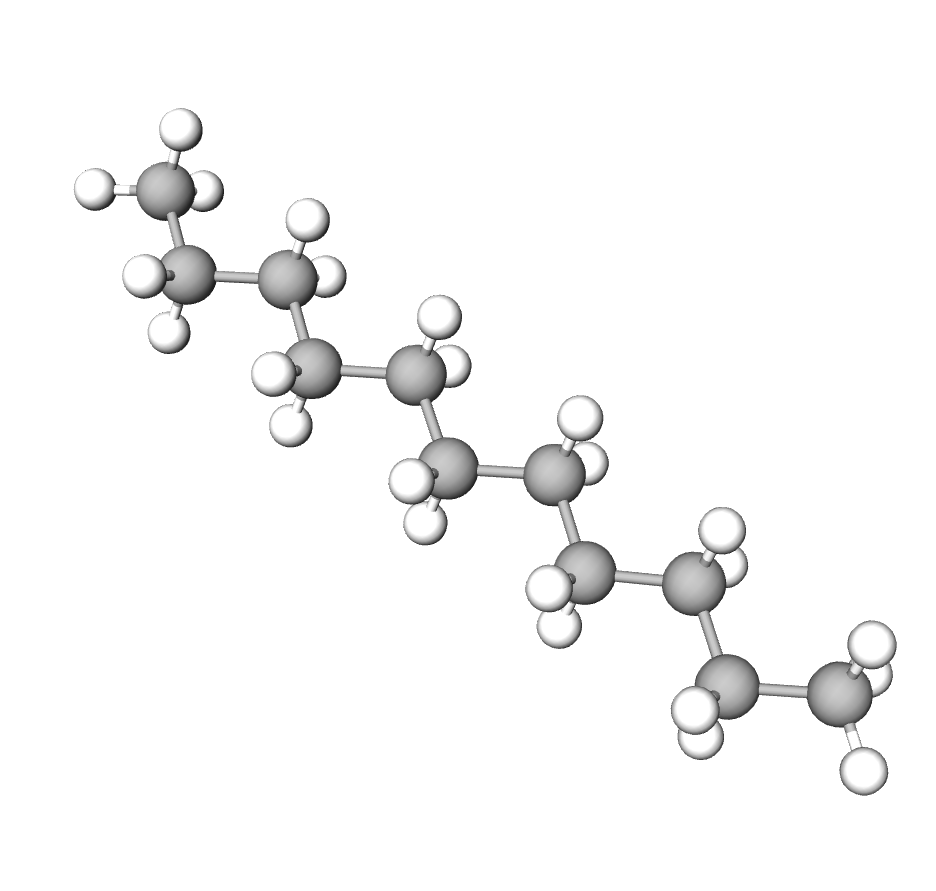
\includegraphics[]{polyethelene.png}
    \caption{Long chain molecule of polyethylene, a common material.}
\end{marginfigure} weakly held together by inter-molecular forces. Initially the molecules are likely to be tangled-up together. As force is applied it is initially difficult to move the polymer chains from this state (\textbf{A}). As the chains begin to unravel they straighten out by bond rotation, requiring relatively little force for a large increase in strain (\textbf{B}). As the polymer chains become straight it becomes much more difficult to extend the material any further without damaging the material (\textbf{C}).

\begin{figure}[ht]
    \begin{center}
        \begin{tikzpicture}[scale=.75]
            \draw[thick, ->] (-0.5,0) -- (11,0) node[anchor=north] {$\epsilon$};
            \draw[thick, ->] (0,-0.5) -- (0,9) node[anchor=east] {$\sigma$};
            \draw (0,0) .. controls (3,7) and (6,1) .. (10,8);
            \draw (1.5,1) node{\textbf{A}};
            \draw (5,1) node{\textbf{B}};
            \draw (8.5,1) node{\textbf{C}};
            \draw[dashed] (3,0) -- (3,3.6);
            \draw[dashed] (7.2,0) -- (7.2,4.7);
        \end{tikzpicture}
    \end{center}
    \caption{Stress-strain curve for a polymer}
    \label{stress-strain-polymer}
\end{figure}

\section{Rubber}
When a rubber is exposed to stress or strain energy, internal rearrangements such as rotation and extension of the polymer chains occur. 
\begin{marginfigure}
    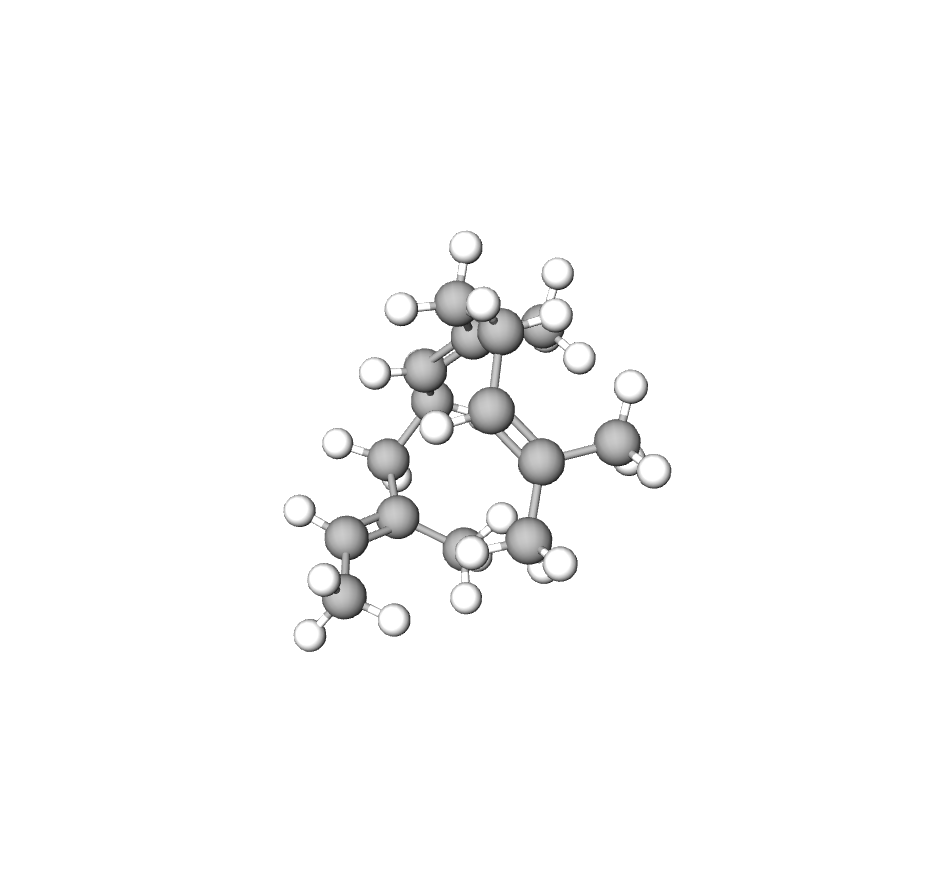
\includegraphics[]{figures/naturalrubber.png}
    \caption{The twisted structure of natural rubber}
\end{marginfigure} These changes occur as a function of the energy applied and the duration and rate of application, as well as the temperature at which the energy is applied.
The difference between the two curves is the hysteresis losses.
\begin{figure}
	\vspace*{-10pt}
	\centering
	\begin{tikzpicture}[scale=0.54]
	\draw[<->] (6.4,0) node[below]{strain} -- (0,0) -- (0,6.4) node[left]{stress};
	\draw[thick,blue,postaction={decorate},decoration={markings,mark=at position 0.5 with {\arrow{>}}}] (0,0) [out=60,in=210] to (3,4) [out=30,in=225] to (6,6);
	\draw[thick,blue,postaction={decorate},decoration={markings,mark=at position 0.5 with {\arrow{>}}}] (6,6) [out=240,in=30] to (3,3) [out=210,in=50] to (0,0);
	\end{tikzpicture}
	\vspace*{-16pt}
\end{figure}
	
\section{End-of-chapter questions}


\subsection*{Springs \& Hooke's law}

\question{A spring has a force constant of $500 \text{ N m}^{-1}$. The spring has a stretch length of 30 cm when a 40 N weight is hung from it. Find the natural length of the spring.}

\question{Two springs, one with spring constant $k_1 = 8.0 \text{ N cm}^{-1}$ and the other with $k_2 = 12 \text{ N cm}^{-1}$. (a) When they are connected in parallel, what is the total extension when the combination supports a load of 60 N? (b) If they are connected in series, what is the total extension when they support the same load?}

\question{A weight of 100 N is placed on top of a spring. The spring is compressed by 2.0 cm. Assume the spring obeys Hooke's law, how much strain energy is stored in the spring?}

\question{A spring with a force constant $800 \text{ N m}^{-1}$ is supported and stands vertically. A ball of mass 60 g falls vertically onto it. The ball has a speed of $3.0\mps$ as it makes contact with the spring. Assume no energy loss, what is the maximum compression of the spring?}

\question{A trolley of mass 160 g is placed on a frictionless track. The trolly pushed against a spring buffer of a force constant $90 \text{ N m}^{-1}$. The spring buffer is compressed by 7.0 cm. The trolley is then released from rest. (a) What is the initial acceleration of the trolley? (b) Assume no loss of energy, what is the final speed of the trolley along the track?}

\question{
	Spring $A$ is stiffer than spring $B$, i.e., $k_A>k_B$. On which spring is more elastic potential energy stored if they are stretched by (a) the same extension, (b) the same force?
}

\begin{marginfigure}
	\vspace*{-5pt}
	\centering
	\begin{tikzpicture}
	\draw[help lines, gray!50, very thin, step=0.1] (0,0) grid (5,4);
	\draw[help lines, step=1] (0,0) grid (5,4);
	\foreach \y in {0,1,2,3, 4} \node[left] at (0,\y) {$\y$};
	\foreach \x in {0,1,2,3,4,5} \node[below] at (\x,0) {$\x$};
	\node at (-1,3.5) {load/kg};
	\node at (4,-0.8) {extension/cm};
	\draw[thick,blue] (0,0) -- (5,3.2);
	\end{tikzpicture}
	\vspace*{-25pt}
\end{marginfigure}

\question{A load is attached to the lower end of a spring. The extension of the spring is measured when the load increases. The variation with extension of the load is shown. (a) Suggest whether the spring obeys Hooke's law. (b) Find the spring constant. (c) How much elastic potential energy is stored in the spring when the extension is 5.0 cm? (d) How much work is done to increase the extension from 2.0 cm to 4.0 cm?}


\question{
	Suppose you have a spring, a ruler, a mass hanger and a set of masses. Suggest how the apparatus may be used to determine the load on the spring at (a) the limit of elasticity, (b) the limit of proportionality?
}


\subsection*{Stress, Strain, \& Young modulus}

\question{A cable of diameter 1.5 mm is under a tension of 200 N. Find the stress in this cable.}

\question{Estimate the stress in your neck when it supports your head in a vertical position.}

\question{A metal wire of natural length 1.8 m and diameter 0.70 mm is fixed to the ceiling at one end. When a mass of 6.5 kg is hung from the lower end, the wire extends by 2.7 mm. (a) Find the strain of the wire. (b) Find the Young modulus of the metal.}

\question{A wire has a diameter of 0.50 mm with a Young modulus of 0.18 TPa. The length of the wire is increased by 0.20\% by a force $F$. (a) Find the stress in the wire. (b) Find the force $F$.}


\question{Two metal wires $A$ and $B$ are made of different materials. The diameter of wire $A$ is twice that of wire $B$, and the Young modulus of wire $A$ is three times that of wire $B$. If the wires are extended by the same strain, what is the ratio of the tension in wire $A$ to tension in wire $B$?}



\question{Two rods $A$ and $B$ of the same diameter are joined end to end and hug vertically. Rod $B$ is twice as long as rod $A$ but has half the Young modulus. When a mass is hung from the combination, what is the ratio of the extension of rod $A$ to the extension of rod $B$?}

\question{Bones of different animals have very similar compositions. Suggest why heavier animals appear to have thicker bones?}


\begin{marginfigure}
	\vspace*{5pt}
	\centering
	\begin{tikzpicture}
	\draw[help lines, gray!50, very thin, step=0.1] (0,0) grid (5,5);
	\draw[help lines, step=1] (0,0) grid (5,5);
	\foreach \y in {0,1,2,3,4,5} \node[left] at (0,\y) {$\y$};
	\foreach \x in {0,0.1,0.2,0.3,0.4,0.5} \node[below] at (10*\x,0) {$\x$};
	\node at (-1,4.5) {$F$/N};
	\node at (4,-0.8) {$x$/mm};
	\draw[thick,blue] (0,0) -- (5,2.4);
	\end{tikzpicture}
	\vspace*{-25pt}
\end{marginfigure}

\question{A load $F$ is suspended from a copper wire. The graph shows the load-extension relation. (a) State two quantities other than $F$ and $x$ that are required to determine the Young modulus of copper. (b) Suggest how the two quantities may be measured. (c) Use the graph to find the energy stored in the wire when a load of 2.0 N is applied. (d) Given that steel has about twice the Young modulus as copper, sketch the variation with $x$ of $F$ for a steel wire that has the same dimensions as the copper wire.}

\begin{marginfigure}
	\vspace*{-10pt}
	\centering
	\begin{tikzpicture}[scale=0.54]
	\draw[<->] (6.4,0) node[below]{strain} -- (0,0) -- (0,6.4) node[left]{stress};
	\draw[thick,blue,postaction={decorate},decoration={markings,mark=at position 0.5 with {\arrow{>}}}] (0,0) [out=60,in=210] to (3,4) [out=30,in=225] to (6,6);
	\draw[thick,blue,postaction={decorate},decoration={markings,mark=at position 0.5 with {\arrow{>}}}] (6,6) [out=240,in=30] to (3,3) [out=210,in=50] to (0,0);
	\end{tikzpicture}
	\vspace*{-16pt}
\end{marginfigure}

\question{
	In an experiment, a speciman of a rubber compound is being stretched and relaxed. The stress-strain curve is plotted. (a) State and explain whether this rubber compound behaves elastically. (b) The tyres on a vehicle are made of this rubber compound. Explain why the tyres become warm as the car travels on a road.
}

%%\chapter{Fluids}

a fluid, such as a liquid or a gas, is a substance that has no fixed shape

unlike a solid, a fluid can flow and yield easily under external force

in this chapter, we will study several aspects of a fluid

\subsection{pressure in a fluid}

\begin{marginfigure}
	\vspace*{-8pt}
	\centering
	\begin{tikzpicture}[yscale=0.75,xscale=0.6]
	\draw[thick,fill=cyan!50] (-2,2.5) arc(180:0:2 and 0.5) -- (2,-2.5) arc(0:-180:2 and 0.5) -- cycle;
	\draw[thick] (2,2.5) arc(0:-180:2 and 0.5);
	\draw (0,2.7) --++ (1,1) node[above]{$A$};
	\draw[<->] (-3,2.5) -- (-3,-2.5) node[left,midway]{$h$};
	\draw[dashed] (-2,2.5) --++ (-2,0);
	\draw[dashed] (-2,-2.5) --++ (-2,0);
	\end{tikzpicture}
	\vspace*{-16pt}
\end{marginfigure}


at a depth of $h$ below surface of a fluid, self-weight of the fluid could produce a pressure


{
	\centering
	
	$ p = \frac{F}{A} = \frac{mg}{A} = \frac{\rho V g}{A} \RA \boxed{p = \rho g h} $
	
}




\cmt pressure in a liquid depends on depth

for different positions in a liquid, as long as they are at same depth, pressure is the same

i.e., pressure does not depend on volume or shape of container

\cmt atmospheric pressure also accounts for total pressure in a liquid

atmosphere presses on surface of a liquid, so total pressure at depth $h$ is: $P=\rho g h + P_\text{atm}$

nevertheless, change in pressure still satisfies: $\Delta p = \rho g \Delta h$

\example{The atmospheric pressure is about $1.0 \times 10^5 \text{ Pa}$. Given that the density of sea water is $1020 \text{ kg m}^{-3}$, what is the total pressure 50 m below the surface of the sea?}

\solc\begin{equation*}
	P = P_\text{atm} + \rho g h = 1.0 \times 10^5 + 1020 \times 9.81 \times 50 \RA P \approx 6.0 \times 10^5 \text{ Pa} 
\end{equation*}

\example{A vertical column of liquid of height 10 m contains both oil and water. The pressure due to the liquids at the bottom of the column is 89 kPa. Given that the density of water is $1000 \text{ kg m}^{-3}$ and the density of the oil is $840 \text{ kg m}^{-3}$. What is the depth of the oil?}

\solc\begin{equation*}
	P = P_\text{oil} + P_\text{water} = \rho_\text{o} g h_\text{o} + \rho_\text{w} g h_\text{w}
\end{equation*}
\begin{equation*}
840 \times 9.81 \times x + 1000 \times 9.81 \times (10-x) = 89\times10^3 \RA x = 5.8 \text{ m} 
\end{equation*}

\begin{marginfigure}
	\vspace*{-4pt}
	\centering
	\begin{tikzpicture}
	\draw[help lines, gray!50, very thin, step=0.2] (0,0) grid (5,4);
	\draw[help lines, step=1] (0,0) grid (5,4);
	\foreach \y/\ylabel in {0/9.70,1/9.75,2/9.80,3/9.85, 4/9.90} \node[left] at (0,\y) {$\ylabel$};
	\foreach \x in {0,5,10,15,20,25} \node[below] at (\x/5,0) {$\x$};
	\node at (-1.2,3.5) {$p$/$10^4$Pa};
	\node at (4,-0.8) {$x$/cm};
	\draw[thick,blue] (0,3.6) -- (4,0);
	\end{tikzpicture}
	\vspace*{-25pt}
\end{marginfigure}

\example{The pressure $p$ of a liquid in a container varies with the height $x$ above the base of the container as shown. The total depth of the liquid is 20 cm. (a) What is the atmospheric pressure? (b) What is the density of the liquid?}

\sol surface of liquid at height $x= 20\text{ cm}$, so 

{
	\centering
	
	$P_\text{atm} = 9.70 \times10^4 \text{ Pa}$
	
}

density of liquid: $\rho = \frac{\Delta p}{g \Delta h} = \frac{(9.88-9.70)\times10^4}{9.81 \times 0.20} \RA \rho \approx 917 \text{ kg m}^{-3}$ \eoe



\subsection{pressure meters}

there are many types of instruments for pressure measurement

we would only focus on two: simple manometers and barometers
\footnote{Some examples of many other types of pressure gauges include
	
\begin{compactitem}
	
	\item[--] mechanical gauges based on metallic pressure-sensing elements
	
	\item[--] electronic gauges based on piezo-resistive effect
	
	\item[--] hot-filament ionization gauges based on ion currents from a gas

\end{compactitem}

Those who are interested are welcome to research into their functions and principles.
}

they both use the fact that $\Delta p = \rho g \Delta h$ within a liquid


\subsection{manometers}

\begin{marginfigure}
	\vspace*{-32pt}
	\centering
	\begin{tikzpicture}[scale=0.9]
	\draw[cyan,fill] (1.5,2) -- (1.5,0) arc(0:-180:1.5) -- (-1.5,1) -- (-1,1) -- (-1,0) arc(-180:0:1) -- (1,2) -- cycle;
	\draw[thick] (1.5,3) -- (1.5,0) arc(0:-180:1.5) -- (-1.5,3)  (-1,3) -- (-1,0) arc(-180:0:1) -- (1,3);
	\draw[<->] (0,1) -- (0,2) node[right, midway] {$\Delta h$};
	\draw[dashed] (-0.8,1) --++ (1.6,0);
	\draw[dashed] (-0.8,2) --++ (1.6,0);
	\draw[thick,->] (-1.25,4) --++ (0,-0.8) node[midway,right]{$P_1$}; 
	\draw[thick,->] (1.25,4) --++ (0,-0.8) node[midway,right]{$P_2$}; 
	\end{tikzpicture}
	\vspace*{-16pt}
\end{marginfigure}

a \keypoint{manometer} consists of a U-shaped tube filled with some liquid

any pressure difference between the two ends of the tube could cause a height difference between liquid levels

for the situation shown, at equilibrium, one has: $P_1 - P_2 = \rho g \Delta h$

if $P_2$ is a reference pressure, then $P_1$ can be calculated

\cmt though any fluid can be used in a manometer, \emph{mercury} is preferred because of its high density ($\rho_\text{Hg} = 1.36 \times 10^4 \text{ kg m}^{-3}$)

\example{A manometer is used to measure the pressure of a gas supply. Side $A$ of the tube is connected to the gas pipe, and the other side $B$ of the tube is open to the atmosphere. If the mercury on side $A$ is higher than on side $B$ by 14 cm, what is the pressure of the gas? (density of mercury: $1.36 \times 10^4 \text{ kg m}^{-3}$; atmospheric pressure: $1.01 \times 10^5 \text{ Pa}$)}

\solc\begin{equation*}
	P_\text{atm} - P_\text{gas} = \rho g h \RA P_\text{gas} = 1.01 \times 10^5 - 1.36 \times 10^4 \times 9.81 \times 0.14 \RA P_\text{gas} \approx 8.23 \times 10^4 \text{ Pa} 
\end{equation*}


\subsection{barometers}

\begin{marginfigure}
	\vspace*{-5pt}
	\centering
	\begin{tikzpicture}[scale=0.9]
	\draw[cyan,fill] (-0.2,6) -- (0.2,6) -- (0.2,0) -- (1,0) -- (1,-0.6) -- (-1,-0.6) -- (-1,0) -- (-0.2,0) -- cycle;
	\draw[thick] (-1,0.3) -- (-1,-0.6) -- (1,-0.6) -- (1,0.3);
	\draw[thick] (-0.2,-0.2) -- (-0.2,7) arc(180:0:0.2) -- (0.2,-0.2);
	\draw (0,3) --++ (-1.2,0.8) node[above]{mercury};
	\draw[<->] (1.5,0) --++ (0,6) node[midway,right]{$h$};
	\draw[dashed] (2,6) -- (0.3,6);
	\draw[dashed] (2,0) -- (1.2,0);
	\end{tikzpicture}
	\vspace*{-16pt}
\end{marginfigure}


take a long glass tube and fill it with mercury

let it stand upside down in a basin

there is atmospheric pressure pushing down on surface of mercury, so a height of mercury is supported up the tube

we can then compute atmospheric pressure by: $P_\text{atm} = \rho g h$

this instrument makes a \keypoint{mercury barometer}

\example{If a mercury barometer supports a height of 760 mm of mercury above the fluid level in the container, what is the atmospheric pressure? If water is used as the barometric liquid, what is the minimum length of the tube required for the same atmospheric pressure? (density of mercury: $1.36 \times 10^4 \text{ kg m}^{-3}$; density of water: $1.00 \times 10^3 \text{ kg m}^{-3}$;)}

\sol atmospheric pressure: $P_\text{atm} = \rho g h = 1.36 \times 10^4 \times 9.81 \times 0.760 \approx 1.01\times10^5 \text{ Pa}$

if mercury is replaced by water: $h' = \frac{P_\text{atm}}{\rho' g} = \frac{1.01\times 10^5}{1000 \times 9.81} \approx 10.3 \text{ m}$ \eoe


\subsection{upthrust}

\begin{marginfigure}
	\vspace*{-8pt}
	\centering
	\begin{tikzpicture}[scale=0.8]
	\draw[thick,fill=cyan!30] (-2,2.5) arc(180:0:2 and 0.5) -- (2,-2.5) arc(0:-180:2 and 0.5) -- cycle;
	\draw[thick] (2,2.5) arc(0:-180:2 and 0.5);
	\draw[thick,fill=brown!60] (-0.8,-0.8) --++ (0,1.2) --++ (0.4,0.4) --++ (1.2,0) --++ (0,-1.2) --++ (-0.4,-0.4) -- cycle;
	\draw[thick] (-0.8,-0.8) ++ (0,1.2) --++ (1.2,0) --++ (0,-1.2);
	\draw[thick] (-0.8,-0.8) ++ (1.2,1.2) --++ (0.4,0.4);
	\draw[thick,dotted] (-0.8,-0.8)--++ (0.4,0.4) --++ (1.2,0);
	\draw[thick,dotted] (-0.8,-0.8) ++ (0.4,0.4) --++ (0,1.2);
	\draw[dashed] (2,2.5) -- (4,2.5);
	\draw[dashed] (0.6,0.6) -- (3.2,0.6);
	\draw[dashed] (0.6,-0.6) -- (4,-0.6);
	\draw[<->] (2.7,2.5) -- (2.7,0.6) node[right,midway]{$h_1$};
	\draw[<->] (3.6,2.5) -- (3.6,-0.6) node[right,midway]{$h_2$};
	\draw[very thick, red, ->] (0,1.4) -- (0,0.6) node[pos=.45, right]{$F_1$};
	\draw[very thick, red, ->] (0,-2) -- (0,-0.6) node[pos=0.65, right]{$F_2$};
	\end{tikzpicture}
%	\vspace*{-16pt}
\end{marginfigure}

now consider a rectangular block immersed in a fluid

top and bottom surface are at different depths, so they experience different pressures

this gives rise to an overall upward force on the cylinder

this force is called the \keypoint{upthrust}: \index{upthrust}
$$ F_U = F_2 - F_1 = \rho g (h_2 - h_1) \times A \RA \boxed{F_U = \rho g V} $$

therefore upthrust exerted on an immersed object equals the weight of the fluid displaced

this is known as the \keypoint{Archimedes' principle} \index{Archimedes' principle}

\cmt origin of upthrust: pressure difference between top and bottom surfaces

\cmt for an object of density $\rho_\text{o}$ immersed in a liquid of density $\rho_\text{l}$

take force in downward direction to be positive, then resultant force acting is:

{
	\centering
	
	$ \fnet = W - F_U = \rho_\text{o} g V - \rho_\text{l} g V = (\rho_\text{o} - \rho_\text{l}) gV$
	
}

\titem if $\rho_\text{o} > \rho_\text{l}$, then $\fnet>0$, resultant force acts downwards, object will sink

\titem if $\rho_\text{o} < \rho_\text{l}$, then $\fnet<0$, resultant force acts upwards, object will rise

\titem if $\rho_\text{o} = \rho_\text{l}$, then $\fnet=0$, object is in equilibrium, it can float at that level

\example{A block of mass 80 g and volume 50 cm$^3$ is suspended from a string into water. When the block is fully immersed and kept at rest, what is the tension in the string?}

\solc\begin{equation*}
	T + F_U = W \RA T = mg - \rho g V = 0.080 \times 9.81 - 1000 \times 9.81 \times 50 \times 10^{-6} \RA T \approx 0.29 \text{ N} 
\end{equation*}

\subsection{end-of-chapter questions}

Data for the questions below where applicable:

\titem density of water: $1.00 \times 10^3 \text{kg m}^{–3}$

\titem density of mercury: $13.6 \times 10^3 \text{kg m}^{–3}$

\titem atmospheric pressure: $1.0\times 10^5 \text{ Pa}$

\subsection*{pressure in a fluid}

\question{
	(a) A dam holds a depth of 50 m of water. What is the water pressure at the base of the dam? (b) Suggest why the walls of a dam must be made thicker near the bottom?
}

\question{
	The deepest trench on Earth is The Mariana Trench located in the Pacific Ocean. The maximum known depth is about 11 km. (a) Assume the sea water has a uniform density of about $1030 \text{ kg m}^{-3}$, estimate the pressure at the base of the trench. (b) The density of sea water actually increases slightly with pressure, suggest how this affects the result you have found.
}

\question{
	Instead of a large viewing window, the window of a submarine is usually of only a few centimetres in diameter. Why is the window made so small?
}

\question{
	If you punch several holes in the bottom of a container filled with water, water will spurt out due to the pressure. Now drop the container, suggest what will happen as it falls freely and defend your explanation.
}

\question{
	Air trapped inside a cylinder is attached to a U-shaped manometer containing mercury. The other side of the manometer is open to  atmosphere. The mercury column on the side open to atmosphere is found to be 45 mm higher, what is the pressure of the trapped air?
}

\begin{marginfigure}
	\vspace*{0pt}
	\centering
	\begin{tikzpicture}[scale=0.8]
	\draw[thick] (0,0) -- (0,3) arc(180:0:0.3) -- (0.6,0) arc(180:315:0.3) --++ (45:6);
	\draw[thick] (0,0) arc(180:315:0.9) --++ (45:6);
	\draw[fill=cyan!50] (0,1) -- (0,0) arc(180:315:0.9) --++ (45:4) --++ (-0.8485,0) --++ (225:3.4) arc(315:180:0.3) -- (0.6,1) -- cycle;
	\draw (0.3,2) --++ (-1,0.8) node[left]{gas};
	\draw[dashed] (0.6,1) -- (5.6,1);
	\draw[dashed] (3,2.192) -- (5.6,2.192);
	\draw[<->] (5.2,1) -- (5.2,2.192) node[midway, right]{20 cm};
	\draw[<->] (2,1) --++ (45:1.7) node[midway, above, rotate=45]{28 cm};
	\end{tikzpicture}
	\vspace*{-12pt}
\end{marginfigure}

\question{The figure shows a pipe closed at one end and open at the other end. Some gas is trapped by a column of mercury as shown. Find the pressure of the gas.}

\question{A water manometer is used to measure the pressure created in a flexible container. Initially, the water columns on each side of the manometer is at the same level. When a girl stands on a 30 cm by 30 cm platform placed on top of the container, a height difference of 50 cm is observed in the manometer. (a) Find the pressure created by the girl. (b) Find the mass of the girl.}

\subsection*{upthrust}

\question{A lead block and an aluminium block of identical size are immersed in water. Upon which block is the upthrust greater?}

\question{
	If somehow the gravitational field on the earth is increased, does a fish sink, float to the surface, or otherwise?
}

\question{
	A diver holds a cube of side 0.30 m and density $800 \text{kg m}^{–3}$ near the seabed. (a) What is the upthrust on the cube? (b) What is its initial acceleration when the cube is released from rest?
}

\question{
	A solid sphere of radius 18 cm and density $2.4 \text{g cm}^{–3}$ is fully submerged in water. A string pulls on the sphere so that the sphere does not sink. (a) Find the tension in the string. (b) If the string is cut, what is the instantaneous acceleration. (c) Describe and explain the acceleration of the sphere as it sinks.
}
\chapter{Waves}

A wave is a way of transferring and storing \emph{energy} without the transport of matter. Most familiar examples are surface waves on water, sound waves, light waves. In the next two chapters, we are going to look at the basics of wave motion and some of the most important wave phenomena.

Wave motion is the propagation of disturbance -- deviations from a state of equilibrium -- from one place to another. 

% Waves consist of continuous oscillations around some fixed locations.

% There are mainly two types of waves, \keypoint{mechanical waves} and \keypoint{electromagnetic waves}. Mechanical waves propagate as oscillations of matter, thus it must travel through a \emph{medium}. Electromagnetic waves can travel in free space.

% A wave can either be \keypoint{transverse} or \keypoint{longitudinal} depending on the direction of its oscillation. The direction of propagation of a transverse wave is perpendicular to the direction of its oscillation, and the wave motion of a longitudinal wave is parallel to its oscillation.

\subsection{Wave terminology}

Wave motion is the propagation of disturbance from one place to another

\begin{figure*}[ht]
	\centering
	\begin{tikzpicture}[xscale=1.2, yscale=0.95]
	\draw [->] (0,-2) -- (0,2.4) node[midway,left]{$O$} node[above]{displacement};
	\draw [->] (0,0) -- (3.1*pi,0) node[below]{position};
	\draw[very thick,->] (1.8*pi,2) -- (2.6*pi,2);
	\node[above,twoline] at (2.2*pi, 2.1) {direction of\\wave motion};
	\foreach \t/\labelcolor in {1/{blue}, 2/{Green}, 3/{purple}, 4/{gray}} {
		\draw[\labelcolor] ({0.4*pi+(\t-1)*0.6)}, 1.7) --++ (0.2,0.5) node[above]{$t_\t$};
		\draw [thick, \labelcolor, domain=0:3*pi, samples=30, smooth] plot (\x,{1.6*sin((\x+0.6-0.6*\t)*1.25 r)});
	}
	\end{tikzpicture}
	
	\caption{wave pattern at different times ($t_1<t_2<t_3<t_4$) as wave travels in space}
\end{figure*}


To describe the wave motion and particle vibrations, we can define the following quantities:

\titem as a wave moves from the source, each point oscillates back and forth about their rest positions. The distance from a particle's equilibrium position is called \keypoint{displacement} of the particle \index{displacement}. The greatest displacement for a particle is called the \keypoint{amplitude} ($A$) \index{amplitude}.

A wave pattern repeats itself over a certain distance, the distance between two adjacent points undergoing exactly same motion is the \keypoint{wavelength} ($\lambda$) \index{wavelength}. One can think of wavelength as crest-to-crest distance, trough-to-trough distance, etc.\footnote{For now, we take for granted that a wave is transverse. There are also longitudinal waves for which terms like crest and trough do not apply. We will get into that in \S\ref{ch-Lwaves}.}

You can also think about how each point also repeats its vibrational motion over a certain time interval. The time for a particle to complete a full oscillation cycle is the  \keypoint{period} ($T$) \index{period}. The number of oscillations for a particle per unit time is the \keypoint{frequency} ($f$) \index{frequency} which can also be defined as the number of crests passing a given point per unit time.\\

The frequency of a wave is related to its period by \begin{empheq}[box=\tcbhighmath]{equation*}{f=\frac{1}{T}}\end{empheq}

The unit of frequency: $[f] = \text{Hz}$ (hertz), where $1 \text{ Hz} = 1 \text{ s}^{-1}$. There's some useful coded language here, many things are ``per second'', the ``Hertz'' part tell you it's probably a wave you're talking about.

\begin{figure*}[ht]
	\centering
	\begin{minipage}{0.48\textwidth}
		\centering
		\begin{tikzpicture}[scale=0.55]
		\draw [->] (0,-2) -- (0,2) node[midway,left]{$O$} node[above]{displacement};
		\draw [->] (0,0) -- (3*pi,0) node[below]{position};
		\draw [very thick,blue,domain=0:3*pi,samples=30,smooth,variable=\x] plot (\x,{1.6*sin(\x*1.25 r)});
		\draw[<->, thick, red] (.4*pi,1.6) -- (.4*pi,0) node[midway,right]{$A$};
		\draw[<->, thick, red] (.4*pi,1.8) -- (2*pi,1.8) node[midway,above]{$\lambda$};
		\end{tikzpicture}
		
		wave pattern of all particles at one instant
	\end{minipage}\hfil
	\begin{minipage}{0.48\textwidth}
		\centering
		\begin{tikzpicture}[scale=0.55]
		\draw [->] (0,-2) -- (0,2) node[midway,left]{$O$} node[above]{displacement};
		\draw [->] (0,0) -- (3*pi,0) node[below]{time};
		\draw [very thick,blue,domain=0:3*pi,samples=30,smooth,variable=\x] plot (\x,{1.6*sin(\x*1.25 r)});
		\draw[<->, thick, red] (.4*pi,1.6) -- (.4*pi,0) node[midway,right]{$A$};
		\draw[<->, thick, red] (.4*pi,1.8) -- (2*pi,1.8) node[midway,above]{$T$};
		\end{tikzpicture}
		
		vibration of one specific particle at all times
	\end{minipage}
\end{figure*}

Wave energy is transferred along the direction of wave motion at a certain speed $v$. In one period, the wave moves forward by a distance of one wavelength, so \keypoint{wave speed} \begin{empheq}[box=\tcbhighmath]{equation*}{v=\frac{\lambda}{T}}\end{empheq}, or in terms of frequency, \begin{empheq}[box=\tcbhighmath]{equation*}{v=\lambda f}\end{empheq}

\example{When a wave travels on a water surface, the maximum depth of water is 21 cm and the minimum depth is 18 cm. What is the amplitude of the wave?}

\begin{soln} The amplitude is half the end-to-end distance: $ A = \frac{1}{2}(21-18) = 1.5 \text{ cm} $ \end{soln}


\example{A wave travelling at $4.0 \mps$ has a wavelength of 50 cm, what is its period?}

\begin{soln} \begin{equation*}
	v = \frac{\lambda}{T} \RA T = \frac{\lambda}{v} = \frac{0.50}{4.0} = 0.125 \text{ s} 
\end{equation*}
\end{soln}

\subsection{Transverse \& longitudinal waves}

A wave can either be \emph{transverse} or \emph{longitudinal}, depending on the direction of its oscillation

\subsection{Transverse waves}

\begin{ilight}
	\centering A \keypoint{transverse} wave has vibrations at right angle to its direction of energy transfer \index{transverse wave}.
\end{ilight}

Examples of transverse waves: 
\titem wave on a string, 
\titem surface wave on water, 
\titem light wave, etc.

For a transverse wave, greatest displacement in positive direction is called a \emph{crest}, or a \emph{peak}, the greatest displacement in negative direction is called a \emph{trough}.


\subsection{Longitudinal waves} \label{ch-Lwaves}

\begin{ilight}
	\centering A \keypoint{longitudinal} wave has vibrations in parallel direction to energy transfer \index{longitudinal wave}.
\end{ilight}

Examples of longitudinal waves: 
\titem sound waves, 
\titem wave along a stretched slinky, etc.

For a longitudinal wave, if medium gets squeezed, we say this region is a \emph{compression}, if a medium expands, we say this region is a \emph{rarefaction}.  The wavelength of a longitudinal wave can be defined as compression-to-compression distance.

\begin{figure*}[ht]
	\centering
	\begin{tikzpicture}[xscale=1, yscale=1.7]
	\foreach \x in {-0.75,-0.5,...,10.75}
	\draw[thick] ({\x} , -1) --++ (0,1);
	\end{tikzpicture}
	
	All particles at their equilibrium position before a pressure wave is set up
\end{figure*}

\begin{figure*}[ht]
	\centering
	\begin{tikzpicture}[xscale=1, yscale=1.7]
	\foreach \x in {-0.75,-0.5,...,11} 
		\draw[thick] ({\x+0.5*cos(\x*0.5*pi r)} , -1) --++ (0,1);
	\foreach \x in {-0.5,-0.25,...,11.25} 
		\draw[thick] ({\x+0.5*cos((\x-1)*0.5*pi r)} , -2.5) --++ (0,1);
	\foreach \x in {-0.5,-0.25,...,11} 
		\draw[thick] ({\x+0.5*cos((\x-2)*0.5*pi r)} , -4) --++ (0,1);
		\foreach \x in {3,7} \node[Green] at (\x,-1.2) {\phantom{p}rarefaction\phantom{p}};
		\foreach \x in {1,5,9} \node[blue] at (\x,-1.2) {compression};
		\foreach \x in {0,4,8} \node[Green] at (\x,-2.7) {\phantom{p}rarefaction\phantom{p}};
		\foreach \x in {2,6,10} \node[blue] at (\x,-2.7) {compression};
		\foreach \x in {1,5,9} \node[Green] at (\x,-4.2) {\phantom{p}rarefaction\phantom{p}};
		\foreach \x in {3,7} \node[blue] at (\x,-4.2) {compression};
		\node at (-1.5,-0.5) {{\large $t_1$}};
		\node at (-1.5,-2) {{\large $t_2$}};
		\node at (-1.5,-3.5) {{\large $t_3$}};
		\draw[very thick,->] (2.8,0.3) -- (7.2,0.3);
		\node[above,twoline] at (5, 0.4) {direction of wave motion};
		\draw[thick,red,<->] (1,-0.5) -- (5,-0.5) node[above,pos=0.55]{$\lambda$};
	\end{tikzpicture}
	
	\caption{compression and rarefaction regions at different times ($t_1<t_2<t_3$)	as a longitudinal pressure wave travels in space}
\end{figure*}



\example{What is the distance between a compression and a rarefaction for a sound wave of frequency 550 Hz? (Speed of sound in air is about $330 \mps$.)}

\begin{soln}\begin{equation*}
	d = \frac{1}{2}\lambda = \frac{v}{2f} = \frac{330}{2\times 550} \RA d = 0.30 \text{ m} 
\end{equation*}
\end{soln}

\subsection{Sound waves}

Sound waves propagate via the compression and rarefaction of air (or other medium) \index{Sound}

Molecules near vibrating source is pushed away from rest positions and into their neighbours, which then in turn push into their neighbours, and so on. In this manner the disturbance is transferred through the medium, forming a sound wave. The sound waves are longitudinal.
	
\begin{figure*}[ht]

\begin{tikzpicture}[scale=1]
\pgfmathsetmacro{\noe}{6}

\foreach \t in {0,0.1,...,14}{
	\pgfmathsetmacro{\np}{pow({1+cos((\t-2)*pi/2.5 r)}, 4)*\noe/4}
	\foreach \idx in {0,1,...,\np} {
		\draw[fill] (\t+rnd*0.1-0.05,rnd*1.8) circle (0.025);	% wave 1
	}
}
\draw[<->,thick] (7,2.4) -- (12,2.4) node[midway,above]{{\footnotesize one wavelength}};
\draw[->,thick] (1,2.4) -- (4,2.4) node[midway,above]{{\footnotesize wave motion}};
\node[below] at (2,-.2) {{\footnotesize compression}};
\node[below] at (7,-.2) {{\footnotesize compression}};
\node[below] at (12,-.2) {{\footnotesize compression}};
\node[below] at (4.5,-.2) {{\footnotesize rarefaction}};
\node[below] at (9.5,-.2) {{\footnotesize rarefaction}};
\end{tikzpicture}
\end{figure*}

Propagation of sound waves require medium (air, water, steel, etc.) which means that sound cannot travel in vacuum. The speed of sound is material-dependent, but not frequency-dependent, for example, sound in general travels faster in denser medium.
	
	\titem $v_\text{air} \approx 340 \mps$ (under standard atmospheric pressure and room temperature)
	
	\titem $v_\text{water} \approx 1500 \mps$
	
	\titem $v_\text{steel} \approx 5000 \mps$
	
The \emph{pitch} of a note is related to frequency of sound wave, rapid vibrations of sound source at high frequencies produce a high pitch. The \emph{loudness} of sound mainly depends on amplitude of vibration. A greater amplitude means the wave is more energetic so it sounds louder.
	
\subsection*{Measurement of sound waves}

Two key apparatuses for sound measurement are the \keypoint{microphone} and the \keypoint{oscilloscope}. \index{oscilloscope}
Sound waves can be captured by a \emph{microphone}, which converts sound into electrical signals, electrical signals can then be sent into an \emph{oscilloscope} (see figure\footnote{The beautiful figure of the oscilloscope was created by \emph{Hugues Vermeiren}, who generously shared the source codes on TeXample: \url{http://www.texample.net/tikz/examples/textronics-oscilloscope/}}) for measurement. The oscilloscope can be thought as an upgraded voltmeter that shows how voltage varies with time.

\begin{figure}[ht]
	\centering
	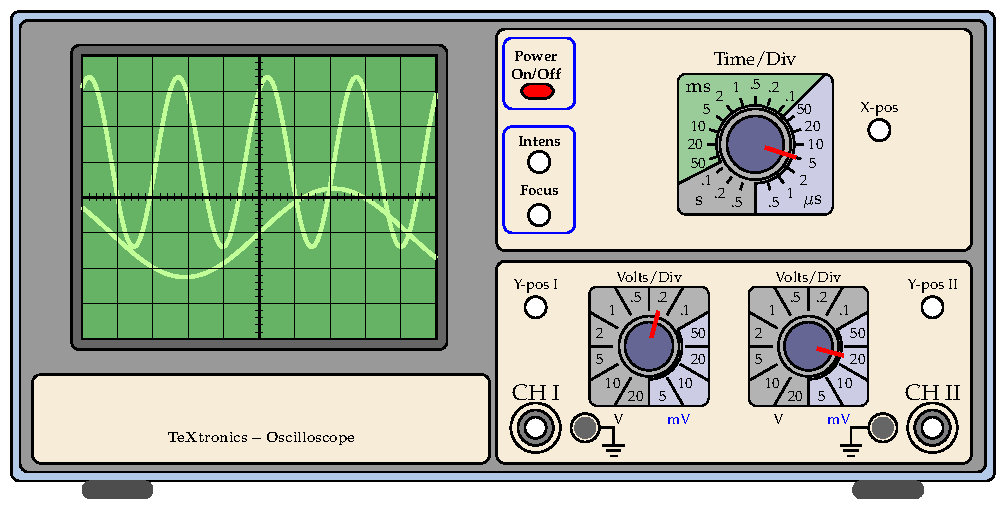
\includegraphics{oscilloscope.pdf}
	\caption{the display and controls of a typical cathode-ray oscilloscope}
\end{figure}

Oscilloscopes displays the variation of voltage ($y$-axis) with time ($x$-axis). The horizontal scale (time axis) is given by \emph{time-base} settings, the vertical scale (voltage axis) is given by \emph{voltage gain}, or \emph{Y-sensitivity} settings. The period $T$ of the sound wave can be found using time-base settings and the frequency calculated by: $f=\frac{1}{T}$. The voltage amplitude can be found using the voltage gain.


\begin{marginfigure}
	\vspace*{-12pt}
	\centering
	\begin{tikzpicture}[scale=0.8]
	\draw[fill=gray!80, rounded corners] (-0.2,-3.2) rectangle (7.2,3.2);
	\draw[Green!50, fill] (0,-3) rectangle (7,3);
	\draw[Green!20, ultra thick, domain=0:7, samples=100] plot (\x, {2*sin((\x-0.6)*120)});
	\draw[black!80, step=1] (0,-3) grid (7,3);
	\end{tikzpicture}
	\vspace*{-16pt}
\end{marginfigure}

\example{A sound wave is detected by a microphone and the trace is displayed on an oscilloscope as shown. If the time-base is set at 0.5 ms div$^{-1}$ and the voltage gain is set at 2 V div$^{-1}$. What is the frequency and the amplitude of the signal?}

\begin{soln} period: $T = 3 \times 0.5 \text{ ms} = 1.5 \times10^{-3} \text{ s}$

\eqyskip frequency: $f = \frac{1}{T} = \frac{1}{1.5 \times10^{-3} \text{ s}} \approx 667 \text{ Hz}$

\eqyskip amplitude: $A = 2 \times 2 \text{ V} = 4.0 \text{ V}$ \end{soln}


\subsection{Electromagnetic waves}

A wave can be either \emph{mechanical} or \emph{electromagnetic}, depending on whether it requires a medium\index{electromagnetic wave}. Waves that require a \emph{medium} to travel are called \keypoint{mechanical waves}, examples are sound waves, water waves, wave on a string, etc.

Mechanical waves on the other hand, involve vibration of matter particles. No medium is needed for propagation of \keypoint{electromagnetic waves} i.e., they can travel in vacuum.

\subsection{Properties of electromagnetic waves}

\titem electromagnetic waves can travel in free space

\titem electromagnetic waves involve vibrations of electric and magnetic fields -- an altering electric field can generate an altering magnetic field, which then further produces a new altering electric field, so on and so forth. Electric and magnetic fields then permeate through space, transferring energy and information.
	
\titem electromagnetic waves are all transverse.
	
\titem vibration of electric fields and magnetic fields are both perpendicular to wave motion.

\begin{figure*}[ht]
	\centering
	\begin{tikzpicture}[xscale=0.72]
	\draw[Green, thick, ->] (0,-2.1) -- (0,2.1) node[left, twoline] {electric\\field};
	\draw[blue, thick, dotted] (0 ,0) -- (0.7, 1.4);
	\draw[blue, thick, ->] (0, 0) -- (-0.7,-1.4) node[left, twolinecap] {magnetic\\field};
	\draw[thick, ->] (-0.3,0) -- (14,0) node[right, twoline]{direction\\ of energy\\transfer};
	\draw[Green, thick, domain=0:13.5, samples=150] plot (\x, {1.6*sin(2*\x r)});
	\draw[blue, thick] plot [smooth] coordinates {
		(0, 0)
		(0.0007, -0.1987)
		(0.0053, -0.3894)
		(0.0177, -0.5646)
		(0.0413, -0.7174)
		(0.0793, -0.8415)
		(0.134, -0.932)
		(0.2073, -0.9854)
		(0.3002, -0.9996)
		(0.4131, -0.9738)
		(0.5454, -0.9093)
		(0.6958, -0.8085)
		(0.8623, -0.6755)
		(1.0422, -0.5155)
		(1.2325, -0.335)
		(1.4294, -0.1411)
		(1.6292, 0.0584)
		(1.8278, 0.2555)
		(2.0213, 0.4425)
		(2.2059, 0.6119)
		(2.3784, 0.7568)
		(2.5358, 0.8716)
		(2.6758, 0.9516)
		(2.7968, 0.9937)
		(2.8981, 0.9962)
		(2.9795, 0.9589)
		(3.0417, 0.8835)
		(3.0864, 0.7728)
		(3.1156, 0.6313)
		(3.1323, 0.4646)
		(3.1397, 0.2794)
		(3.1415, 0.0831)
		(3.1417, -0.1165)
		(3.1442, -0.3115)
		(3.1529, -0.4941)
		(3.1715, -0.657)
		(3.2032, -0.7937)
		(3.2506, -0.8987)
		(3.316, -0.9679)
		(3.4007, -0.9985)
		(3.5053, -0.9894)
		(3.6296, -0.9407)
		(3.7727, -0.8546)
		(3.9328, -0.7344)
		(4.1075, -0.5849)
		(4.2939, -0.4121)
		(4.4886, -0.2229)
		(4.6876, -0.0248)
		(4.8872, 0.1743)
		(5.0832, 0.3665)
		(5.272, 0.544)
		(5.4499, 0.6999)
		(5.6139, 0.8278)
		(5.7614, 0.9228)
		(5.8905, 0.9809)
		(6, 1)
		(6.0896, 0.9792)
		(6.1597, 0.9193)
		(6.2114, 0.8228)
		(6.2468, 0.6935)
		(6.2683, 0.5366)
		(6.2791, 0.3582)
		(6.2828, 0.1656)
		(6.2832, -0.0336)
		(6.2842, -0.2315)
		(6.2899, -0.4202)
		(6.304, -0.5921)
		(6.3298, -0.7404)
		(6.3704, -0.8592)
		(6.4282, -0.9437)
		(6.5047, -0.9906)
		(6.601, -0.998)
		(6.7172, -0.9657)
		(6.8526, -0.8948)
		(7.0059, -0.7883)
		(7.1749, -0.6503)
		(7.3568, -0.4864)
		(7.5484, -0.3031)
		(7.7461, -0.1078)
		(7.946, 0.0919)
		(8.144, 0.2879)
		(8.3362, 0.4724)
		(8.5191, 0.6381)
		(8.6892, 0.7784)
		(8.8438, 0.8876)
		(8.9807, 0.9614)
		(9.0985, 0.9969)
		(9.1963, 0.9927)
		(9.2744, 0.9488)
		(9.3336, 0.8672)
		(9.3755, 0.751)
		(9.4024, 0.6048)
		(9.4173, 0.4346)
		(9.4235, 0.247)
		(9.4248, 0.0495)
		(9.4251, -0.1499)
		(9.4283, -0.3433)
		(9.4385, -0.5231)
		(9.459, -0.682)
		(9.4932, -0.8137)
		(9.5435, -0.9129)
		(9.6121, -0.9758)
		(9.7001, -0.9998)
		(9.808, -0.9839)
		(9.9356, -0.9288)
		(10.0817, -0.8367)
		(10.2444, -0.7112)
		(10.4213, -0.5573)
		(10.6094, -0.3813)
		(10.805, -0.19)
		(11.0044, 0.0089)
		(11.2037, 0.2073)
		(11.3988, 0.3976)
		(11.586, 0.5719)
		(11.7617, 0.7235)
		(11.9231, 0.8462)
		(12.0676, 0.9352)
		(12.1935, 0.9869)
		(12.2996, 0.9993)
		(12.3859, 0.9718)
		(12.4528, 0.9056)
		(12.5016, 0.8033)
		(12.5345, 0.6689)
		(12.5539, 0.5079)
		(12.5633, 0.3266)
		(12.5662, 0.1324)
		(12.5664, -0.0672)
		(12.568, -0.2641)
		(12.5748, -0.4504)
		(12.5906, -0.6188)
		(12.6187, -0.7626)
		(12.6621, -0.8759)
		(12.7229, -0.9543)
		(12.8027, -0.9946)
		(12.9023, -0.9954)
		(13.0218, -0.9564)
		};
	\end{tikzpicture}
	\caption{variation in electric and magnetic fields for an electromagnetic wave}
\end{figure*}

Note that all electromagnetic waves travel at a constant speed $c=3.0\times10^8\mps$ in free space i.e., speed of light in vacuum is constant\footnote{The speed of light in vacuum is actually a \emph{universal} physical constant. According to Einstein's special relativity, this is the upper limit for the speed at which matter and information can travel. This speed is also independent of the inertial reference frame one chooses, i.e., the speed of light in vacuum is the same for all observers, regardless of the motion of the source or the observer.}


\newpage
\subsection{The electromagnetic spectrum}

Electromagnetic waves come in a wide range of wavelengths and frequencies, the distribution of electromagnetic radiation according to wavelength or frequency is the \keypoint{electromagnetic spectrum}\index{electromagnetic spectrum} (see diagram)



\begin{figure*}[!ht]
	\centering
	\begin{tikzpicture}[yscale=1.04]
	% define visible spectrum shading
	\pgfdeclareverticalshading{visible}{100bp}
	{color(0bp)=(violet!70); color(25bp)=(violet!70); color(35bp)=(blue!70);
		color(45bp)=(green!70); color(55bp)=(yellow!70); color(65bp)=(orange);
		color(75bp)=(red); color(100bp)=(red)}
	% grayish background for spectrum labels
	\draw[gray!15,fill] (-1.5,-8) rectangle (1.5,7.5);
	% axes
	\draw (-1.5,-8) -- (-1.5,7.5) (1.5,-8) -- (1.5,7.5);
	\node at (-3,7.7) {wavelength};
	\node at (3,7.7) {frequency};
	% spectrum labels
	\shade[shading=visible] (-1.5,-1.15) rectangle (1.5,-0.75);
	\foreach \x/\xlabel in {1.8/{radio waves}, -2/{microwaves}, -4.6/{infrared}, -6.35/{visible light}, -7.8/{ultraviolet}, -11/{X-rays}, -14.8/{$\gamma$-rays} } \node at (0,{\x*0.7+3.5}) {\xlabel};
	% values of wavelengths
	\foreach \x in {5,3,1,...,-15} {
		\draw (-1.5,{\x*0.7+3.5}) --++ (-0.5,0);
		\node at (-3,{\x*0.7+3.5}) {$10^{\x}$ m};
	}
	% values of frequencies
	\foreach \x in {3,5,...,23} {
		\draw (1.5,{-\x*0.7+8.8}) --++ (0.5,0);
		\node at (3,{-\x*0.7+8.8}) {$10^{\x}$ Hz};
	}
	% dashed lines as separators
	\foreach \x in {-1,-3,-9,-13} \draw[dashed,thick] (-1.5,{\x*0.7+3.5}) --++ (3,0);
	% extension for visible spectrum
	\draw[thick, gray!75] (1.5,-1.15) --++ (3,0) -- (5,-3);
	\draw[thick, gray!75] (1.5,-0.75) --++ (3,0) -- (5,1);
	\shade[shading=visible] (5,-3) rectangle (7,1);
	\node at (6, 1.3) {visible light};
	\node[right] at (7.2, 0.8) {700 nm};
	\node[right] at (7.2, -2.8) {400 nm};
	\end{tikzpicture}
	\caption{the electromagnetic spectrum}
\end{figure*}

\newpage

The table below shows electromagnetic spectrum in somewhat more precise details \footnote[][-2cm]{There are no precise accepted boundaries between different ranges in the electromagnetic spectrum. The boundaries are actually somewhat ambiguous. The ranges of different portions tend to overlap. For example, a large portion of the ranges of X-rays overlap with that of $\gamma$-rays, and microwaves are considered by many people as a subdivision of radio waves. Therefore, the values given here are merely supposed to give you some rough idea about the order of magnitudes for electromagnetic wavelengths and frequencies. So the point I want to make here is: do not take the borderlines too seriously.}
\vspace{3cm}
\begin{figure*}
\begin{center}
	\begin{tabular}{|C{4cm}|C{4cm}|C{4cm}|}
		\hline Region of spectrum & Range of wavelength & Range of frequency \\ 
		\hline radio waves  & 10$^{-1}$ $\sim$ 10$^{6}$ m & 10$^{2}$ $\sim$ 10$^{9}$ Hz \\ 
		\hline microwaves & 10$^{-3}$ $\sim$ 10$^{-1}$ m & 10$^{9}$ $\sim$ 10$^{11}$ Hz \\ 
		\hline infra-red & 7$\times$10$^{-7}$ $\sim$ 10$^{-3}$ m & 10$^{11}$ $\sim$ 10$^{14}$ Hz \\ 
		\hline visible light  & 4$\times$10$^{-7}$ $\sim$ 7$\times$10$^{-7}$ m & 10$^{14}$ $\sim$ 10$^{15}$ Hz \\ 
		\hline ultraviolet & 10$^{-9}$ $\sim$ 4$\times$10$^{-7}$ m & 10$^{15}$ $\sim$ 10$^{17}$ Hz \\ 
		\hline X-rays & 10$^{-13}$ $\sim$ 10$^{-9}$ m & 10$^{17}$ $\sim$ 10$^{19}$ Hz \\ 
		\hline $\gamma$-rays & 10$^{-16}$ $\sim$ 10$^{-11}$ m & 10$^{19}$ $\sim$ 10$^{24}$ Hz\\ 
		\hline
	\end{tabular} 
\end{center}
\end{figure*}

Each type of electromagnetic waves has important applications in some area
\footnote{The entries listed here only include a teeny-weeny part of the uses of electromagnetic radiation, somewhat based on my personal taste. I also included a handful of explanations for the examples that I found interesting (otherwise I would not choose them), as you will see a huge load of footnotes in the next few pages. You are encouraged to do some researches as well, I can guarantee that you will not be disappointed.}

\begin{compactitem}
	\item[--] Radio waves.
	
	\xskip Telecommunication (TV/radio broadcast, satellite communication). Having the longest wavelengths of all radiation, radio waves have the best ability to diffract around obstacles in city buildings and mountains, therefore a large area can be covered.

	\item[--] Microwaves.
	
	\xskip Telecommunication (mobile phones, WiFi, Bluetooth, satellite communication). Microwaves do not diffract sufficiently as radio waves, but they can transmit more information per unit time because they have higher frequencies. Microwaves are used in short-range telecommunication, including mobile phones, wireless networks, and bluetooth connections.
		
		
	\xskip Heating food (microwave ovens). Frequency of microwaves are close to the natural frequencies of the rotational motion of water molecules. When food is exposed to microwaves, the water molecules in the food resonate and vibrate more violently, causing a rise in the food's temperature.
	
	\item[--] Infrared (IR).
	
	\xskip IR thermography (temperature monitors, thermographic cameras). All objects emit electromagnetic radiation based on their temperatures. According to the law of black-body radiation, objects near room temperature emit thermal energy as infrared radiation, so variations in the temperature can be detected.
	
	\xskip Night-vision devices. Night-vision devices convert photons (just think of them as particles of light for now) into electrons, which are amplified by a chemical and electrical process and then converted back into visible light. Infrared sources can be used to augment the available light, increasing the visibility in the dark.
	
	\xskip IR heating (IR heat lamps, IR saunas). 	
	\xskip IR data transmission (remote controls, optical-fibre communication)	
	\item[--] Visible Light
	
	\xskip Human Vision. Human eyes are only sensitive to a small fraction of the electromagnetic spectrum. The wide variety of colours that we see is actually built up from the relative intensities of red, green and blue light collected by the three colour detectors in our eyes.
	
	\item[--] Ultraviolet (UV).
	
	\xskip UV sterilising (drinking water treatment, disinfection of medical facilities, etc.) Short-wavelength UV light can damage the DNA's in living organisms. A microorganism exposed to germicidal UV light might not be able to reproduce, and becomes harmless. For the same reason, overexposure to UV radiation present in the sunlight can cause sunburn, or even skin cancer.
		
	\xskip Fluorescent dyes (black light fluorescent paint, UV watermarks) UV radiation can cause many substances to glow through chemical reactions. UV watermarks that are visible under UV light are used to prevent counterfeiting of currency, or forgery of important documents such as passports and ID cards.
	
	\item[--] X-rays.
	
	\xskip Medical imaging (X-ray imaging, CT scans). X-rays are very energetic and thus very penetrating. They can pass through human body easily to form an image giving information about the structures of tissues and bones.
	
	\xskip Security checking (luggage scanners).
	
	\xskip X-ray crystallography. X-rays can be diffracted by the lattice of atoms in a crystal. The diffraction pattern gives information about the structure of the lattice. X-ray crystallography is a very important experimental technique to study the microscopic structures of new materials.
	
	\item[--] $\gamma$-rays.
	
	\xskip Radiation therapies (cancer treatment). $\gamma$-rays have extremely high frequencies. They are even more energetic and penetrating. They can be used to damage the DNA of cancerous tissue, and hence kill the cancerous cells as a treatment.
	
	\xskip Medical imaging (PET scans). Positron emission tomography (PET) uses a radioactive tracer to produce $\gamma$-rays within the tissues of interest. The energy and location of these $\gamma$-rays can be detected and sent to a computer to build up a 3D image of the body part.
\end{compactitem}
\newpage
\example{A beam of electromagnetic radiation is known to have a frequency of 25 THz in vacuum. What is its wavelength?}

\begin{soln}
    
\begin{equation*}
	\lambda = \frac{c}{f} = \frac{3.00\times10^8}{25\times10^12} \RA \lambda = 1.2 \times 10^{-5} \text{ m} \quad \text{(infra-red)} 
\end{equation*}
\end{soln}

	

\subsection{Wave intensity}

Energy can be transmitted along a wave, the degree to which this energy is concentrated is called the intensity of the wave. In this case ``concentration'' has two meanings -- concentration in time and concentration in area $S$\footnote{To avoid confusion, I reserved letter `$A$' for wave amplitude and chose `$S$' to represent an area.}

\begin{ilight}
	\centering \keypoint{intensity} of a wave is defined as the power $P$ per unit area on a cross section $S$: \begin{empheq}[box=\tcbhighmath]{equation*}{I=\frac{P}{S}}\end{empheq}\index{wave intensity}
\end{ilight}

The unit of wave intensity is Watts per meter: $[I] = \text{ W m}^{-2}$

\sidenote[][]{\piste The intensity is proportional to square of its amplitude: $\boxed{I \propto A^2}$}.

The intensity of a wave decreases as it spreads out in space, in fact Intensity is a great example of the \emph{inverse square law}. Intensity at distance of $r$ from a point source is inversely proportional to $r^2$: $\tcbhighmath{I \propto \frac{1}{r^2}}$
\footnote{As a wave produced from a point source travels out by a distance $r$ away from the source, the energy it carries is spread uniformly over the surface area of the sphere of radius $r$, that is: $S=4\pi r^2$. So the intensity of a wave obeys an inverse square law: $I \propto \frac{1}{r^2}$.}

\example{If the amplitude of an incoming wave is increased by 50\%, what is the increase in the wave intensity?}

\begin{soln} $I \propto A^2 \RA \frac{I'}{I} = \left( \frac{A'}{A} \right)^2 = \left( 1 + 50\% \right)^2 =2.25 \RA $ so intensity is increased by 125\% \end{soln}

\example{Two observers $A$ and $B$ are at a distance $r_A$ and $r_B$ from a point source where $r_A=2r_B$. (a) Find the ratio of their intensities $\frac{I_A}{I_B}$. (b) Find the ratio of their amplitudes $\frac{A_A}{B_B}$.}

\begin{soln}

{
	\centering
	
	$ I \propto \frac{1}{r^2} \RA \frac{I_A}{I_B} = \left(\frac{r_B}{r_A}\right)^2 = \left(\frac{1}{2}\right)^2 \RA \frac{I_A}{I_B} = \frac{1}{4} $
	
	\vspace*{0.4em} $ I \propto A^2 \RA \frac{A_A}{A_B} = \sqrt{\frac{I_A}{I_B}} = \sqrt{\frac{1}{4}} \RA \frac{A_A}{A_B} = \frac{1}{2} $
	
}

\end{soln}


\subsection{Polarisation}

\subsection{Plane polarisation}

\begin{ilight}
	A wave is \keypoint{plane-polarised}, or simply \keypoint{polarised}, if the vibration is in one single direction at right angle to the direction of propagation of energy\index{polarisation}
\end{ilight}

\begin{figure}[ht]
	\centering
	\begin{minipage}{0.45\textwidth}
		\centering
		\begin{tikzpicture}[scale=0.64]
		\draw[very thick, blue, ->] (210:2) -- (30:8) node[twoline, above, black]{direction of\\energy transfer};
		\foreach \t in {0,45,90,135} {
			\draw[red, ultra thick, <->] (\t:1.5) --++ ({\t+180}:3);
			\draw[red, ultra thick, <->] (30:3.5) ++ (\t:1.5) --++ ({\t+180}:3);
		}
		\end{tikzpicture}
		
		an unpolarised wave
		
		(wave vibrations in multiple directions)
	\end{minipage}\hfil
	\begin{minipage}{0.45\textwidth}
		\centering
		\begin{tikzpicture}[scale=0.64]
		\draw[very thick, blue, ->] (210:2) -- (30:8) node[twoline, above, black]{direction of\\energy transfer};
		\foreach \t in {90} {
			\draw[red, ultra thick, <->] (\t:1.5) --++ ({\t+180}:3);
			\draw[red, ultra thick, <->] (30:3.5) ++ (\t:1.5) --++ ({\t+180}:3);
		}
		\end{tikzpicture}
		
		a plane-polarised wave
		
		(wave vibrations in one direction only)
	\end{minipage}
\end{figure}

Polarisation\footnote[][-10cm]{\piste Apart from plane polarisation where the vibrations are fixed in a single direction, there are also \emph{circular} or \emph{elliptical} polarisation, for which the direction of vibrations \emph{rotate} in a plane as the wave travels.} is a phenomenon associated with \emph{transverse} waves only. Longitudinal waves (such as sound waves) cannot be polarised because longitudinal vibrations are always parallel to direction of energy transfer.

One of the most important examples are polarisation of \emph{electromagnetic waves}. Sunlight, light emitted from incandescent bulbs etc is unpolarised because they are emitted randomly from their sources, so they contain all planes of polarisation. Lasers, diodes, microwave antennae and a few others produce polarised emissions. 
A few of the great many applications of polarisation are:

\begin{compactitem}
	\item[--] polarising sunglasses \& photography \sidenote[][-10cm]{When unpolarised light is reflected at the boundary of two media, the reflected beam would become partially polarised. Polarising sunglasses use this effect to reduce the sunlight reflected from shiny surfaces, such as a lake (for sightseeing tourists) or road surfaces (for drivers). For the same reason, photographers often place a polarising filter in front of the camera lens to darken skies and increase the contrast.}
	
	\item[--] polarised 3D films\footnote[][-6.5cm]{The eyeglasses worn by viewers contain a pair of polarising filters with mutually perpendicular axes. When two images are projected onto the same screen, each filter restricts the light reaching each eye by passing only one of the images that is polarised in the same direction. This creates an 3D illusion.}
	
	\item[--] liquid-crystal display (LCD) technology\footnote[][-4cm]{Liquid crystal arrays can be realigned by applying an electric field. This causes the axis of polarization to rotate, hence backlight may be allowed to pass or be blocked, forming dark patterns of the display.}
	
	\item[--] radio transmission and reception\footnote[][-2cm]{Since electric currents flow in certain directions only, so the radio waves and microwaves produced from aerials are intrinsically polarised. This means the reception of signals would be sensitive to a particular direction, but totally insensitive to the normal direction. This explains why altering the orientation of antennas could greatly enhance the quality of reception.}
\end{compactitem}

\subsection{Polarisers \& Malus's law}

A plane-polarised light can be produced from unpolarised light using a \keypoint{polariser}.

A polariser blocks vibrations in all planes except the plane of polarisation. This type of polariser, often called a \emph{linear absorptive polariser}, is basically a synthetic transparent plastic sheet made of certain crystals. The thin sheet contains long-chain organic molecules aligned parallel to each other. When an unpolarised light passes through the polariser, there is a strong absorption of the electric field parallel to the alignment of molecules, so vibration of the electric field is allowed to pass in one direction only.

The direction along which vibration is allowed to pass is called the axis of the polariser

\begin{figure*}[ht]
	\centering
	\begin{tikzpicture}[scale=0.65]
	\draw[very thick, blue, ->] (0,0) -- (10,0);	
	\draw[fill=cyan!30] (0,0) ++ (0,2) ++ (160:2) --++ (-20:4) --++ (0,-4) --++ (160:4) --++ (0,4);
	\foreach \t in {-1.5,-1,...,1.5} \draw[very thin, gray!80, decorate, decoration={snake, amplitude=0.6}] (0,0) ++ (0,\t) ++ (160:1.6) --++ (-20:3.2);
	\draw[thick, Green, dashed] (0,1.8) -- (0,-1.8);
	\draw[Green] (0.1,1.2) -- (1.6,3) node[black, right, twoline]{axis of\\transmission};
	\draw[gray!80] (-1.4,1.6) -- (-3,3) node[black, left, twoline]{direction of alignment\\of molecules};
	\draw[very thick, blue] (-10,0) -- (0,0);
	\foreach \t in {-20,40,90,125} {
		\draw[red, ultra thick, <->] (-4,0) ++ (\t:1.5) --++ ({\t+180}:3);
		\draw[red, ultra thick, <->] (-8,0) ++ (\t:1.5) --++ ({\t+180}:3);
	}
	\foreach \t in {4,8} \draw[red, ultra thick, <->] (\t,-1.5) --++ (0,3);
	\node at (-6,-3.2) {unpolarised light};
	\node at (6,-3.2) {plane-polarised light};
	\node at (0,-3.2) {polariser};
	\end{tikzpicture}
	
	\caption{unpolarised light goes through a polariser and becomes plane-polarised}
\end{figure*}

Polarised light can be sent through a second polarising filter (sometimes called an \emph{analyser})


\begin{figure*}[ht]
	\centering
	\begin{minipage}{0.45\textwidth}
		\centering
		\begin{tikzpicture}[scale=0.4]
		\draw[very thick, blue, ->] (3,0) -- (8.4,0);	
		\draw[fill=orange!30] (3,0) ++ (0,2) ++ (160:2) --++ (-20:4) --++ (0,-4) --++ (160:4) --++ (0,4);
		\foreach \t in {-1.5,-1,...,1.5} \draw[very thin, gray!80, decorate, decoration={snake, amplitude=0.6}] (3,0) ++ (0,1.5) ++ (160:\t) --++ (0,-3);	
		\draw[very thick, blue] (-3,0) -- (3,0);	
		\draw[fill=cyan!30] (-3,0) ++ (0,2) ++ (160:2) --++ (-20:4) --++ (0,-4) --++ (160:4) --++ (0,4);
		\foreach \t in {-1.5,-1,...,1.5} \draw[very thin, gray!80, decorate, decoration={snake, amplitude=0.6}] (-3,0) ++ (0,\t) ++ (160:1.6) --++ (-20:3.2);	
		\draw[very thick, blue] (-8.4,0) -- (-3,0);
		\foreach \t in {-20,40,90,125} {
			\draw[red, very thick, <->] (-6.5,0) ++ (\t:1.5) --++ ({\t+180}:3);
		}
		\foreach \t in {0} \draw[red, very thick, <->] (\t,-1.5) --++ (0,3);
		\node at (-3,-3.5) {polariser};
		\node at (3,-3.5) {analyser};
		\end{tikzpicture}
		
		no transmission of light if polariser and 
		
		analyser are aligned at right angles
	\end{minipage}\hfil
	\begin{minipage}{0.45\textwidth}
		\centering
		\begin{tikzpicture}[scale=0.4]
		\draw[very thick, blue, ->] (3,0) -- (8.4,0);	
		\draw[fill=orange!30] (3,0) ++ (0,2) ++ (160:2) --++ (-20:4) --++ (0,-4) --++ (160:4) --++ (0,4);
		\foreach \t in {-1.5,-1,...,1.5} \draw[very thin, gray!80, decorate, decoration={snake, amplitude=0.6}] (3,0) ++ (0,\t) ++ (160:1.6) --++ (-20:3.2);	
		\draw[very thick, blue] (-3,0) -- (3,0);	
		\draw[fill=cyan!30] (-3,0) ++ (0,2) ++ (160:2) --++ (-20:4) --++ (0,-4) --++ (160:4) --++ (0,4);
		\foreach \t in {-1.5,-1,...,1.5} \draw[very thin, gray!80, decorate, decoration={snake, amplitude=0.6}] (-3,0) ++ (0,\t) ++ (160:1.6) --++ (-20:3.2);	
		\draw[very thick, blue] (-8.4,0) -- (-3,0);
		\foreach \t in {-20,40,90,125} {
			\draw[red, very thick, <->] (-6.5,0) ++ (\t:1.5) --++ ({\t+180}:3);
		}
		\foreach \t in {0,6.5} \draw[red, very thick, <->] (\t,-1.5) --++ (0,3);
		\node at (-3,-3.5) {polariser};
		\node at (3,-3.5) {analyser};
		\end{tikzpicture}
		
		polarised light is unaffected if polariser
		
		and analyser are aligned in parallel
	\end{minipage}
\end{figure*}

If polarised light of initial intensity $I_0$ has an angle $\theta$ to the axis of analyser then \keypoint{Malus's law}\footnote{\piste This isn't actually on the spec but it's pretty critical so we often include it.}\index{Malus's law} states that transmitted intensity is given by: $$\tcbhighmath{I = I_0 \cos^2 \theta}$$

This is because only electric field parallel to axis of analyser is transmitted, so transmitted amplitude\footnote{This is actually the amplitude of the electric field strength.} satisfies: $A = A_0 \cos\theta$, where $A_0$ is the initial amplitude.

Recall that intensity is proportional to square of amplitude, so $I = I_0 \cos^2 \theta $

\example{A beam of light polarised in the vertical direction has an amplitude $A$ and intensity $I$. It passes through a polarising filter whose axis of polarisation is at $45^\circ$ to the vertical. (a) What is the amplitude and the direction of polarisation of the emerging beam? (b) If the emerging beam then enters another filter whose axis of polarisation is at $75^\circ$ to the vertical, what is the amplitude and intensity of the emerging beam?}

\begin{soln} through first filter: 
$A_1 = A \cos\theta_1 = A \cos 45^\circ \RA A_1 = \frac{1}{\sqrt{2}} A $
light is polarised in a direction at $60^\circ$ to the vertical

through second filter:
$A_2 = A_1 \cos\theta_2 = \frac{1}{\sqrt{2}} A \times \cos (75^\circ - 45^\circ) \RA A_2 = \frac{\sqrt{6}}{4} A $

$I_2 = \left(\frac{\sqrt{6}}{4} \right)^2 I \RA I_2 = \frac{3}{8} I$

 or, $I_2 = I \cos^2\theta_1 \cos^2 \theta_2^2 = I \times \cos^2 45^\circ \times \cos^2 (75^\circ-45^\circ) \RA I_2 = \frac{3}{8} I$ 

\end{soln}




\subsection{Doppler effect}

\begin{ilight}
	Relative motion between wave source and the observer causes a change in observed frequency, this is known as the \keypoint{Doppler effect}\index{Doppler effect}
\end{ilight}

Any type of wave can exhibit Doppler effect - we are extremely familiar with the changes in pitch as a car drives toward, alongside, then away from us. When wave source moves towards observer, a higher frequency is observed and when wave source moves away from observer, a lower frequency is observed. We can see clearly the direction in which these ducklings are swimming thanks to the same physics:
\begin{figure}
    \centering
    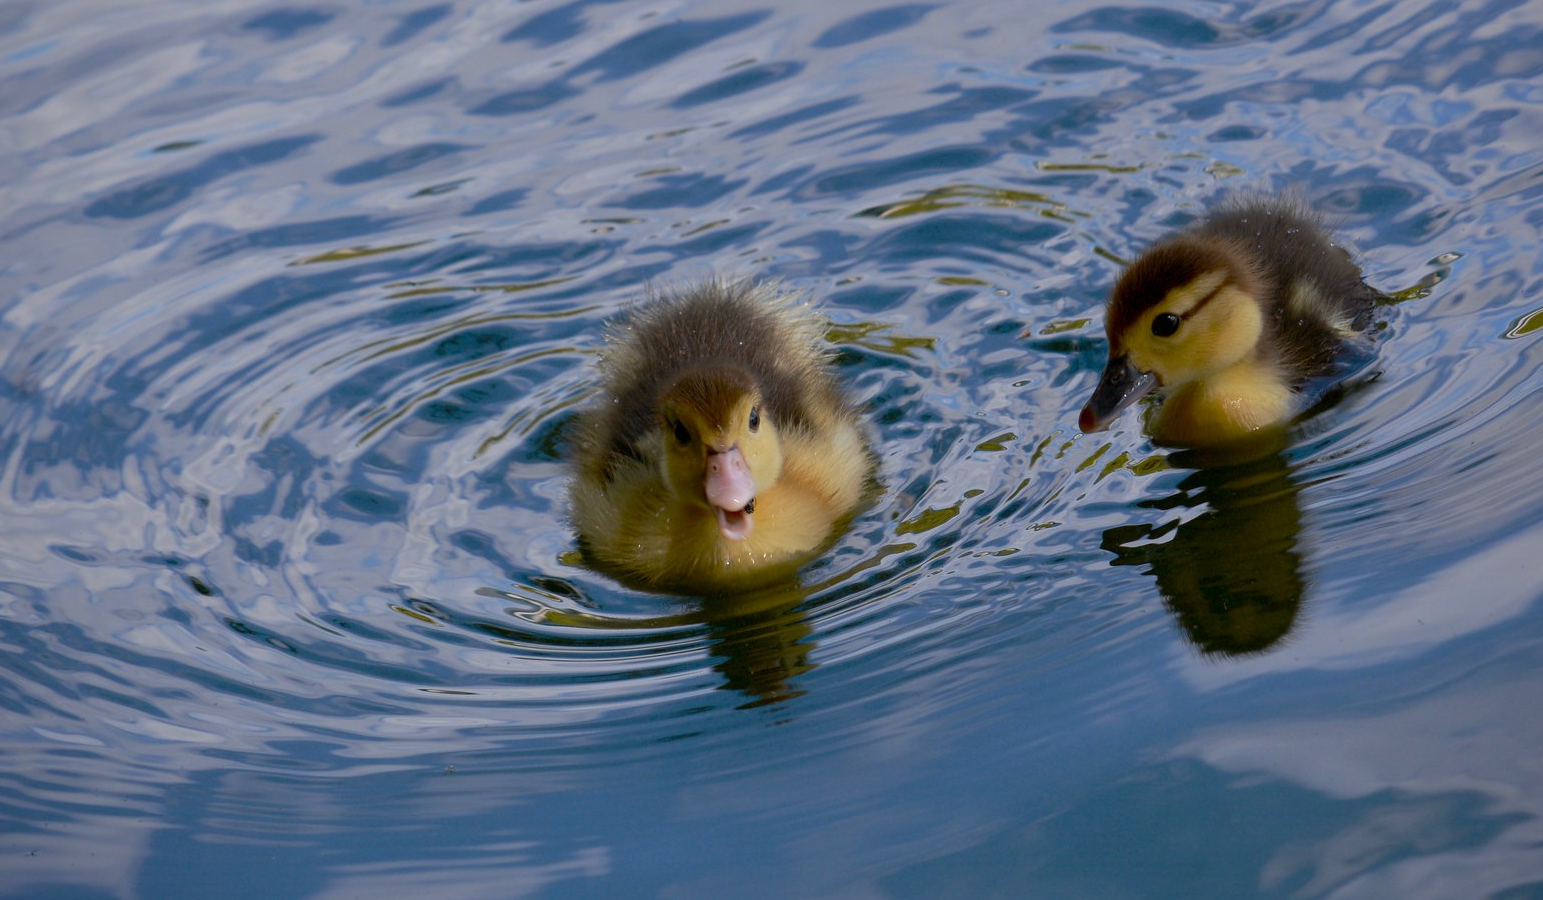
\includegraphics[width=0.75\linewidth]{figures/Swimduck.png}
    \caption{Doppler Ducks...}
    \label{fig:enter-label}
\end{figure}

The Doppler effect also occurs if source is at rest but observer is in motion, as long as there is \emph{radial} motion between source and observer, there is shift in frequency.

Doppler effect finds its use in many areas, some examples are

\begin{compactitem}
	\item[--] \emph{Doppler radars}: used to measure velocity of moving target (speeding cars, tennis balls, etc.)
	
	\item[--] \emph{Doppler ultrasonography}: used to image blood flow in human bodies
	
	\item[--] \emph{Astronomy}: used to study motion of stars and galaxies
\end{compactitem}

\newpage

\subsection*{Explanation of the Doppler effect}

Suppose wave source is moving towards the observer at speed $v_s$, at time $t=0$, the source emits a wavefront which travels at speed $v$.

\begin{figure*}[ht]
	\centering
	\begin{tikzpicture}[scale=0.95]
	\draw[thick] (0,0) circle (0.2);
	\draw[fill] (12,0.4) circle (0.2);
	\draw[ultra thick] (12,0.2) -- (12,-0.1) -- (11.8,-0.6) (12,-0.1) -- (12.2,-0.6) (11.75,-0.1) -- (12,0.15) -- (12.25,-0.1);
	\draw[blue,thick] (0.4, 0.62513) arc (10:-10:3.6);
	\node at (0,-1) {source};
	\node at (12,-1) {observer};
	\end{tikzpicture}
\end{figure*}

After one period, the wavefront travels forward by a distance of $vT$. At same time, source moves forward by a distance of $v_s T$ and emits a new wavefront:

\begin{figure*}[ht]
	\centering
	\begin{tikzpicture}[scale=0.95]
	\draw[thick,gray!80] (0,0) circle (0.2);
	\draw[thick] (2,0) circle (0.2);
	\draw[gray, ->] (0.3,0) -- (1.7,0);
	\draw[fill] (12,0.4) circle (0.2);
	\draw[ultra thick] (12,0.2) -- (12,-0.1) -- (11.8,-0.6) (12,-0.1) -- (12.2,-0.6) (11.75,-0.1) -- (12,0.15) -- (12.25,-0.1);
	\draw[Green,thick] (2.4, 0.62513) arc (10:-10:3.6);
	\draw[blue,thick] (6.4, 0.62513) arc (10:-10:3.6);
	\draw[gray!80,dashed,thick] (0.4, 0.62513) arc (10:-10:3.6);
	\node at (0,-1) {source};
	\node at (12,-1) {observer};
	\draw[<->] (2.55,-1.5) -- (6.5,-1.5) node[above, midway]{$\lambda'$};
	\draw[<->] (0.5,-1.5) -- (2.45,-1.5) node[above, midway]{$v_s T$};
	\draw[<->] (0.5,-2.4) -- (6.5,-2.4) node[above, midway]{$\lambda = vT$};
	\end{tikzpicture}
\end{figure*}

If the source is at rest, observer simply perceives a wavelength $\lambda = vT$.
If the source is moving closer, a shorter wavelength $\lambda'$ is perceived since frequency is inversely proportional to wavelength, so higher frequency $f'$ is observed. Similar discussion would follow for the case where source moves away from observer.

The change in observed frequency is due to change in wavelength caused by relative motion - if source moves towards/away from observer, apparent wavelength becomes shorter/longer.

\subsection*{Doppler effect equation}

We are now ready to derive an equation for the shift of observed frequency. 
Quantitatively, we can write: $\lambda' = \lambda \mp v_s T \quad$ ("$-$"/"$+$" if source is moving closer/away).


Using $v = \lambda f$ and $f=\frac{1}{T}$, this becomes: $ \frac{v}{f'} = \frac{v}{f} \mp \frac{v_s}{f} $.
rearranging, one finds observed frequency is given by: $$\tcbhighmath{f' = f\frac{v}{v \mp v_s}}$$

\example{A police car moving towards you at $16 \mps$ sirens at 500 Hz. Given that the speed of sound in air is $340\mps$, at what frequency do you hear the siren?}

\begin{soln}
\begin{equation*}
	f' = f\frac{v}{v - v_s} = 500 \times \frac{340}{340-16} \RA f' \approx 525 \text{ Hz} 
\end{equation*}
    
\end{soln}

    

\example{A star emits an $H_\alpha$ line of wavelength 656 nm. (a) What is the frequency of this $H_\alpha$ line? (b) An observer on earth detects a wavelength of 680 nm, what can we say about motion of the star? (c) Find the relative speed of the star with respect to the earth.}

\begin{soln}
The original frequency of $H_\alpha$: $f = \frac{c}{\lambda} = \frac{3.00\times10^8}{656 \times 10^{-9}} \approx 4.57 \times 10^{14} \text{ Hz}$

The observed wavelength is longer (redshift), this means the star is moving away, or receding.

To find speed of star, we can consider observed frequency: $f' = \frac{c}{\lambda'} = f\frac{c}{c + v_s}$
\begin{equation*}
	\frac{3.00\times10^8}{680\times10^{-9}} = 4.57 \times 10^{14} \times \frac{3.00\times10^8}{3.00\times10^8 + v_s} \RA v_s \approx 1.10 \times 10^7 \mps
\end{equation*}

alternatively, we can consider observed wavelength: $\lambda' = \lambda + v_s T$, or: $\Delta \lambda = \lambda' - \lambda = \frac{v_s}{f}$
\begin{equation*}
	(680-656)\times10^{-9} = \frac{v_s}{4.57 \times 10^{14}} \RA  v_s \approx 1.10 \times 10^7 \mps 
\end{equation*}
\end{soln}


% \chapter{Waves} \label{chapter:Waves}


% \section{Superposition}\syl{state, explain and use the principle of superposition}
% When two or more waves arrive at the same place at the same time they combine with each other according to the principle of superposition.

% % \begin{marginfigure}\superpositionpic{60}{0}{1.5}{1.5}\caption{Constructive interference}\end{marginfigure}

% This states that the resultant displacement at any point is equal to the sum of the displacements of the individual waves.  Note that a displacement may be negative so addition of two displacements may result in a resultant, which is smaller than either of the original displacements.//
% When two waves of equal amplitude and wavelength meet in phase they interfere constructively to produce a new wave of twice the amplitude but the same wavelength\syl{state the conditions necessary for two-source interference to be
% observed, i.e. constant phase difference, vibrations in the same line}
% .

% When two waves of equal amplitude and wavelength meet in antiphase they interfere destructively to cancel each other out.
% % \begin{marginfigure}\superpositionpictwo{60}{180}{1.5}{-1.5}\caption{destructive interference}\end{marginfigure}

% When two waves of equal amplitude and wavelength meet with any other phase difference the resultant will have an intermediate amplitude.
% % \begin{marginfigure}{\superpositionpic {60}{60}{1.5}{1.5}}\caption{Two waves, out of phase}\end{marginfigure}

% \section{Coherence}

% Coherence\syl{give examples of coherent and incoherent sources,} is an essential condition for the interference of waves.  Two sources of waves are described as coherent if they emit waves with a constant phase difference (note that the waves do not necessarily have to be in phase).  Two waves arriving at a point are said to be coherent if there is a constant phase difference between them as they pass that point.

% \section{Interference} Interference cannot be observed with light - or any form of electromagnetic radiation - from two separate light sources.  This is because the phase difference between light waves from the two sources changes randomly so the points of cancellation and reinforcement move about at random.  The two sets of waves need to be produced from a single source, either:
% \begin{itemize} \item by dividing the wavefront and arranging for the divided wavefronts to overlap, as in the double slit experiment (see below) or \item dividing the amplitude of the waves using a partial reflector and arranging for the separated waves to overlap, as in thin film interference.
% \end{itemize}
% \subsection{Path difference and Interference} 
% \newif\ifstartcompletesineup
% \newif\ifendcompletesineup
% \pgfkeys{
%     /pgf/decoration/.cd,
%     start up/.is if=startcompletesineup,
%     start up=true,
%     start up/.default=true,
%     start down/.style={/pgf/decoration/start up=false},
%     end up/.is if=endcompletesineup,
%     end up=true,
%     end up/.default=true,
%     end down/.style={/pgf/decoration/end up=false}
% }
% \pgfdeclaredecoration{complete sines}{initial}
% {
%     \state{initial}[
%         width=+0pt,
%         next state=upsine,
%         persistent precomputation={
%             \ifstartcompletesineup
%                 \pgfkeys{/pgf/decoration automaton/next state=upsine}
%                 \ifendcompletesineup
%                     \pgfmathsetmacro\matchinglength{
%                         0.5*\pgfdecoratedinputsegmentlength / (ceil(0.5* \pgfdecoratedinputsegmentlength / \pgfdecorationsegmentlength) )
%                     }
%                 \else
%                     \pgfmathsetmacro\matchinglength{
%                         0.5 * \pgfdecoratedinputsegmentlength / (ceil(0.5 * \pgfdecoratedinputsegmentlength / \pgfdecorationsegmentlength ) - 0.499)
%                     }
%                 \fi
%             \else
%                 \pgfkeys{/pgf/decoration automaton/next state=downsine}
%                 \ifendcompletesineup
%                     \pgfmathsetmacro\matchinglength{
%                         0.5* \pgfdecoratedinputsegmentlength / (ceil(0.5 * \pgfdecoratedinputsegmentlength / \pgfdecorationsegmentlength ) - 0.4999)
%                     }
%                 \else
%                     \pgfmathsetmacro\matchinglength{
%                         0.5 * \pgfdecoratedinputsegmentlength / (ceil(0.5 * \pgfdecoratedinputsegmentlength / \pgfdecorationsegmentlength ) )
%                     }
%                 \fi
%             \fi
%             \setlength{\pgfdecorationsegmentlength}{\matchinglength pt}
%         }] {}
%     \state{downsine}[width=\pgfdecorationsegmentlength,next state=upsine]{
%         \pgfpathsine{\pgfpoint{0.5\pgfdecorationsegmentlength}{0.5\pgfdecorationsegmentamplitude}}
%         \pgfpathcosine{\pgfpoint{0.5\pgfdecorationsegmentlength}{-0.5\pgfdecorationsegmentamplitude}}
%     }
%     \state{upsine}[width=\pgfdecorationsegmentlength,next state=downsine]{
%         \pgfpathsine{\pgfpoint{0.5\pgfdecorationsegmentlength}{-0.5\pgfdecorationsegmentamplitude}}
%         \pgfpathcosine{\pgfpoint{0.5\pgfdecorationsegmentlength}{0.5\pgfdecorationsegmentamplitude}}
% }
%     \state{final}{}
% }



% One way of demonstrating interference effects is to take a single source of waves (s) and allow the waves to travel by two different paths to a detector (D).

% \begin{figure*}
% \begin{center}
% \begin{tikzpicture}

% \tikzset{interface/.style={
%         % The border decoration is a path replacing decorator. 
%         % For the interface style we want to draw the original path.
%         % The postaction option is therefore used to ensure that the
%         % border decoration is drawn *after* the original path.
%         postaction={draw,decorate,decoration={border,angle=-45,
%                     amplitude=0.3cm,segment length=2mm}}}}
                    
% \tikzset{waveo/.style={decorate, draw=red,
%         decoration={complete sines,amplitude=20pt, segment length=10pt, start up, end down}}}
% \tikzset{wavet/.style={decorate, draw=blue,
%         decoration={complete sines,amplitude=20pt,start up, end up, segment length=10pt}}}
%         \tikzset{wavetr/.style={decorate, draw=blue,
%         decoration={complete sines,amplitude=20pt,start up, end down, segment length=10pt}}}
% \draw[dashed] (0,0)-- (5,-4)-- (10,0)node[anchor=west,text width=4cm]{Detector, D};
% \draw[waveo] node [anchor=east]{Source, S}(0,0) -- node[midway, fill=white]{Path $\vec{SR}$}(4.7,-4) (5.3,-4)  node[anchor=south, fill=white]{Mirror, R}-- (10,0)node[midway, sloped, fill=white]{Path $\vec{RD}$};
% \draw[wavet] (0,0)-- (10,0);
% \draw[thick] (10,2)--(10,-3);
% \draw[dashed] (0,0)-- (10,0) node[midway,sloped, fill=white]{Path $\vec{SD}$};
% \draw[thick, interface](4,-4)--(6,-4);
% \end{tikzpicture}
% \caption{Illustrating path difference.}
% \end{center}

% \end{figure*}

% This can be done as shown below by having one path directly from S to D and another path via a reflector (R).  The path difference\syl{show an understanding of path difference, phase difference, and
% coherence} is the difference between the distances travelled, SD and SRD.

% As R is moved perpendicular to the direction $\vec{SD}$ a point will be reached where the direct wave and the reflected wave arrive at D in phase.  At this point constructive interference occurs at D and a maximum amplitude is detected.  (Note that this occurs when the path difference has a value like $\frac{1}{2}$ or $\frac{3}{2}$ wavelengths as a phase change of $\frac{1}{2}$ cycle occurs on reflection.)

% If R is moved away from the line $\vec{SD}$ the path difference increases and a point is reached where the direct and reflected waves arrive in antiphase.   A minimum amplitude is now detected.  The amplitude will not in general be zero as the amplitude of the reflected wave will be less than that for the direct wave as it has travelled further so complete cancellation will not occur.

% Further movement of R away from $\vec{SD}$ will restore the maximum amplitude as the two waves will again be in phase.  The increase in the length $\vec{SRD}$ that occurs in moving from one maximum to the next is one wavelength and this provides a method for measuring wavelength.

% \section{Single slit diffraction}
% In general it is considered that light only travels in straight lines - evidence for example is the production of shadows. When water waves pass through a gap or past an object they spread into the "shadow" region as shown below (A). This is known as "diffraction". The width of the opening controls the degree of diffraction. A narrow opening causes more diffraction (B).

% \subsection{Diffraction through a single narrow slit:}

% If  the slit is more than a few millimetres wide, a sharp rectangular shadow is formed (C). 
% If the slit is narrowed (D) the pattern begins to change - a wide central band is observed with a series of bright fringes either side. The central band is twice the width of the outer fringes. As the slit approaches its narrowest, the pattern broadens and becomes less bright (due to cutting down of light able to pass through slit).

% If white light is used the central band is white, however, the fringes are coloured.
% If monochromatic (single wavelength/colour) light is used the central band and fringes are the same colour. Red light has a more spread out pattern than blue - it also has a larger wavelength than blue - diffraction increases with wavelength.

% Intensity distribution of pattern\syl{recall the shape of the intensity pattern from a single slit and its effect
% on double-slit and diffraction grating patterns}:
% The diagram below (fig: \ref{single}) shows a typical diffraction pattern obtained when monochromatic light passes through a single narrow slit. Also plotted is the intensity of the pattern.

% \begin{figure}
% \label{single}
% 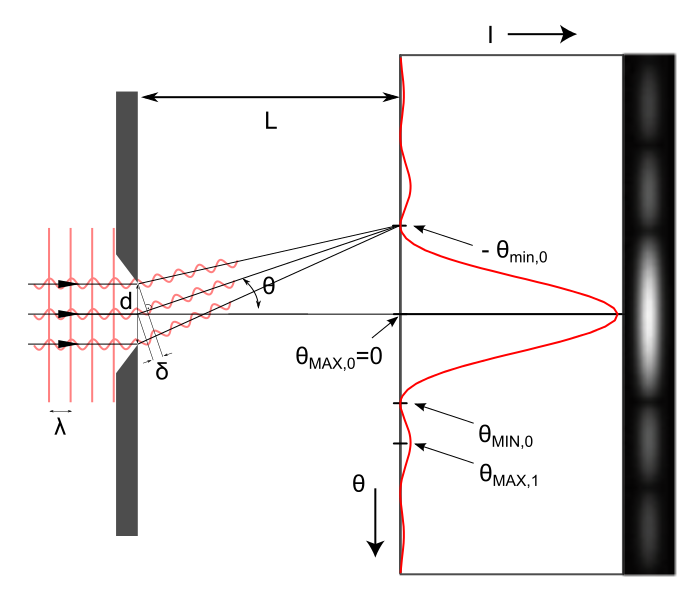
\includegraphics[]{Single.png}
% \caption{Single slit diffraction pattern and geometry. }
% \end{figure}

% The central peak has the greatest intensity, with decreasing intensity with each fringe either side. Each band/fringe has its greatest intensity in its centre. This is the point where light is most likely to fall in its range.
% The fringes are caused by the edges of the slit acting like two wave sources, the waves from the two wave "sources" interfere superimposing an interference pattern over the diffraction pattern.	 

% \section{Youngs experiment} 
% The modern double-slit experiment is a demonstration that light and matter can display characteristics of both classically defined waves and particles; moreover, it displays the fundamentally probabilistic nature of quantum mechanical phenomena. A simpler form of the double-slit experiment was performed originally by Thomas Young in 1801. He believed it demonstrated that the wave theory of light was correct and his experiment is sometimes referred to as Young's experiment or Young's slits. The experiment belongs to a general class of "double path" experiments, in which a wave is split into two separate waves that later combine into a single wave. Changes in the path lengths of both waves result in a phase shift, creating an interference pattern.
% \begin{figure*}
% \begin{tikzpicture}
% \tikzset{waveo/.style={decorate, draw=red,
%         decoration={complete sines,amplitude=20pt, segment length=10pt, start up, end up}}}
% \tikzset{wavet/.style={decorate, draw=blue,
%         decoration={complete sines,amplitude=20pt,start up, end up, segment length=10pt}}}
%         \tikzset{wavetr/.style={decorate, draw=blue,
%         decoration={complete sines,amplitude=20pt,start up, end down, segment length=10pt}}}
% \draw (0,0) -- (0,-.5);
% \draw (0,0) -- (0,.5);
% \draw (0,.8)-- (0,1.5);
% \draw (0,-.8)-- (0,-1.5);
% \draw[dashed] node [anchor=north east]{A} (0,.65)-- (10,0)node[anchor=west,text width=4cm]{Constructive interference. Path lengths $=n\lambda$};
% \draw[waveo] (0,.65)-- (10,0);
% \draw[waveo] (0,-.65)-- (10,0);
% \draw[thick] (10,2)--(10,-3);
% \draw[dashed] (0,.65)-- (10,-2);
% \draw[dashed] node [anchor=south east]{B}(0,-.65)-- (10,-2);
% \draw[wavetr] (0,.65)-- (10,-2) node[anchor=west, text width=4cm]{Destructive interference. Path lengths differ by $\frac{n}{2}\lambda$};
% \draw[wavet] (0,-.65)-- (10,-2);
% \draw[dashed] (0,-.65)-- (10,0) node[midway, fill=white]{Path};

% \end{tikzpicture}
% \caption{Constructive and destructive interference as a result of path differences.}
% \end{figure*}

% The position of the bright and dark fringes is determined by the geometry of the experimental set-up.The distance from center to bright spot n is:
%  \[y = \frac{n \lambda D}{d}\]
% We know that the maxima will be at angles such that the path difference will be whole number of wavelengths. The geometric derivation is shown below.\syl{describe an experimental demonstration of two-source interference for light, appreciating the historical importance of Young's experiment, and be familiar with experiments which demonstrate two source interference for water waves, sound waves and microwaves;} 

% \begin{figure}[!ht]
% 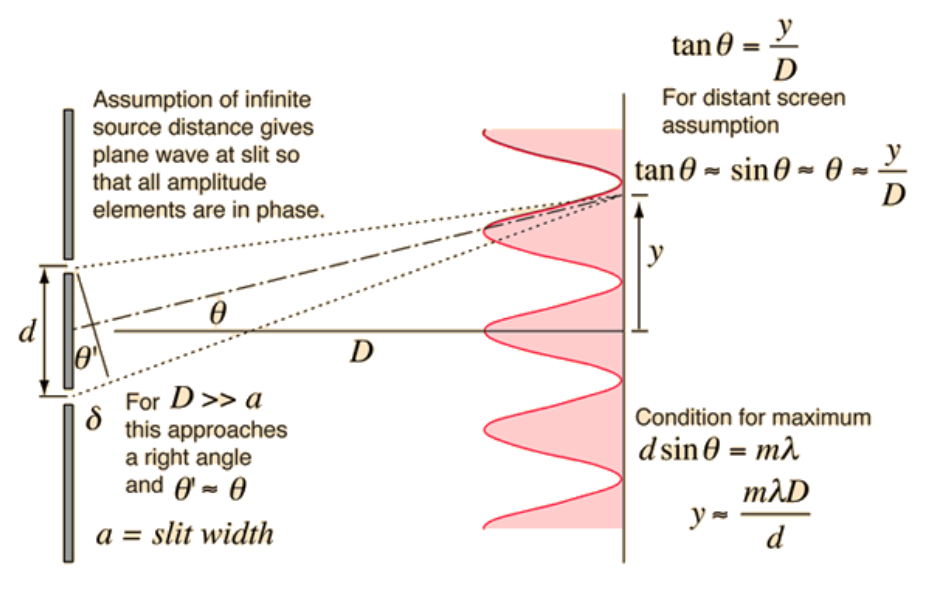
\includegraphics[]{twin.PNG}
% \caption{Beam pattern and geometric workings for Young's slits}
% \end{figure}

% Note that this makes use of the small angle approximation, a useful simplification of the basic trigonometric functions which is approximately true in the limit where the angle approaches zero.\begin{marginfigure}
% 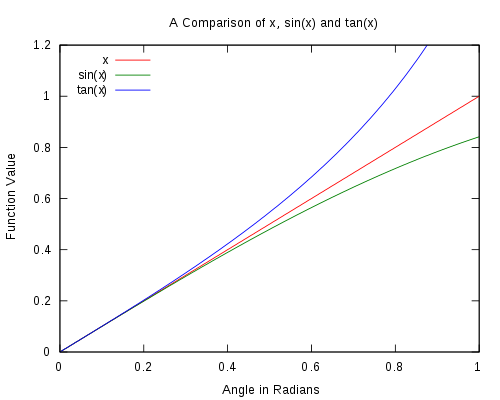
\includegraphics[]{small.png}
% \caption{Illustrating the small angle approximation}
% \end{marginfigure} They are truncations of the Taylor series for the basic trigonometric functions to a second-order approximation.

% \section{Diffraction grating}

% A diffraction grating is usually a piece of glass or plastic with closely-spaced lines on it. A transmission grating has thin clear spaces/slits where light can pass through, while a reflection gratings have shiny surfaces between the lines that reflect light.
% The tracks on a compact disc are very close together - the shiny gaps between the lines act as a reflection grating, leading to a colourful light spectrum being formed when light reflects off the surface.
% Transmission gratings are used to measure wavelengths of light to a very high degree of accuracy (spectrometer) - all substances have characteristic absorption/emission spectra.

% \subsection{Explaining diffraction gratings:}

% The individual lines act like wave sources or thin slits - they produce diffracting waves which will then interfere. Destructive interference leads to cancellation in nearly all directions - there are a few very clearly defined directions where constructive interference occurs, leading to bright fringes. The direction of these fringes depends on the wavelength of light - the wavelength can thus be determined!

% \paragraph{Diffraction grating formula} 

% Parallel rays of monochromatic light of wavelength ``$\lambda$'' fall on a diffraction grating with slit separation/grating spacing ``d''.

% \begin{marginfigure}
% 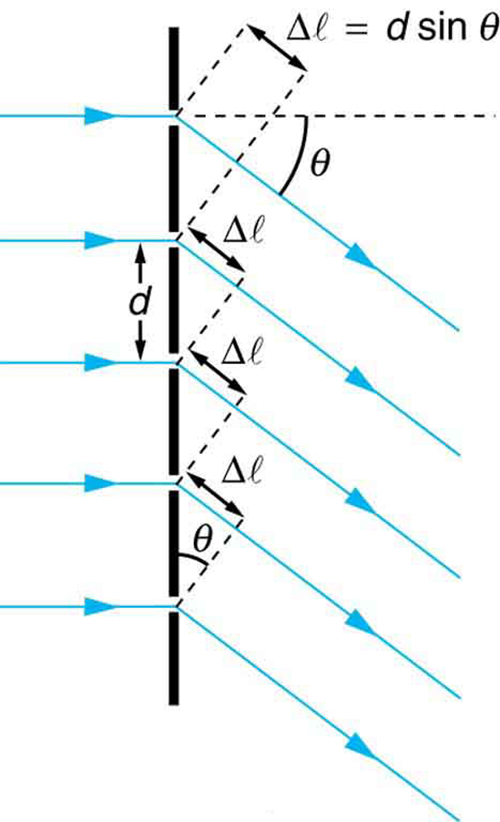
\includegraphics[scale=.5]{grating.jpg}
% \end{marginfigure}

% If the grating has $N$ lines per metre, the grating spacing is given by; $$d=\frac{1}{N}$$\syl{use the equation $d sin\theta = n\lambda$ for a diffraction grating}

% For constructive interference light from adjacent slits must be in phase (with light from all slits/lines).

% $\Delta l= d sin \theta$, where $\theta$ is the angle of diffraction

% Hence $$d sin\theta = n\lambda$$


% \section{Standing Waves}
% Standing or stationary waves\syl{understand that a stationary wave can be regarded as a superposition of two progressive waves of equal amplitude and frequency,travelling in opposite directions and that the internodal distance is $\frac{\lambda}{2}$}
%  are a superposition effect, which occurs when two identical waves (implying waves with a similar amplitude and frequency) travelling in opposite directions interfere.  The most common example of this is where incident and reflected waves interfere, for example on a spring or in a pipe in a musical instrument.

% With a string, spring or pipe of fixed length there will be certain frequencies where a standing wave pattern is produced as shown below.  These frequencies will be those which give an integral number of half wavelengths within the fixed length.  The standing wave is produced by interference of the waves travelling in both directions caused by reflection at the ends. See the diagram on the right.  

% It is characterised by nodes, which are points of zero displacement, and antinodes, which are points of maximum displacement.  The first few possible patterns for transverse waves on a string or spring are shown below.
% \begin{figure*}
% \begin{tikzpicture}[x={(1cm,0.5cm)},z={(0cm,1cm)},y={(1cm,-0.2cm)}]

%         %repere
%         \draw[->] (0,-pi,0) --++ (6,0,0) node[above right] {Frequency};
%         \draw[->] (0,-pi,0) --++ (0,6.5,0) node[right] {Time};
%         \draw[->] (0,-pi,0) --++ (0,0,1.5);        
%             %sinusoides
%             \draw[blue] plot[domain = -pi:+pi, samples = 300] 
%             (1,\x,{0.3*cos(10*.5/10*(\x) r)});
%             \draw[blue] (1,-pi-0.15,0) node [left]{$f_{0}$};
           
%             \draw[blue,dashed] plot[domain = -pi:+pi, samples = 300] 
%             (1,\x,{-0.3*cos(10*.5/10*(\x) r)});
%             \draw[blue] (0,-pi-0.15,0);
            
%             \draw[blue] plot[domain = -pi:+pi, samples = 300] 
%             (3,\x,{0.3*sin(10*1/10*(\x) r)});
%             \draw[blue] (3,-pi-0.15,0) node [left]{$f_{1}$};
%              \draw[blue,dashed] plot[domain = -pi:+pi, samples = 300] 
%             (3,\x,{-0.3*sin(10*1/10*(\x) r)});
%             \draw[blue] (3,-pi-0.15,0);
            
%             \draw[blue] plot[domain = -pi:+pi, samples = 300] 
%             (5,\x,{0.3*cos(10*1.5/10*(\x) r)});
%             \draw[blue] (5,-pi-0.15,0) node [left]{$f_{2}$};
%             \draw[blue,dashed] plot[domain = -pi:+pi, samples = 300] 
%             (5,\x,{-0.3*cos(10*1.5/10*(\x) r)});
%             \draw[blue] (5,-pi-0.15,0);
             
       
%     \end{tikzpicture}
% \end{figure*}  
% The separation of adjacent nodes or antinodes is half a wavelength.  The different numbers of half wavelengths on the spring or string correspond to different allowed frequencies.  The lowest of these (on the left) is called the fundamental.  The others are whole number multiples of the fundamental frequency and are called harmonics.  Each subsequent frequency is known as an overtone. Because of the phase change on reflection at the fixed ends the ends are both nodes.

% The wavelength can be found by measuring the node separation and doubling it.  This gives a method for finding the speed of sound or electromagnetic waves if the frequency is known, using v = f.  For example, if a standing wave is set up using 1 GHz radio waves and the node separation is found to be 0.15 m the wavelength will be 0.30 m and the wave speed is given by:

% $$c = f \times \lambda= (1 \times 10^{9} Hz) \times  0.30 m = 3 \times 10^{8} ms^{-1}$$

% \section{Standing Waves in Musical Instruments}

% Stringed instruments such as violins and pianos produce standing waves as described above.  Hitting, plucking or bowing the string produces waves, which travel off in both directions.  The pitch of the fundamental and therefore of the harmonics may be increased by reducing the length of the string, by increasing the tension in it or by using a lighter string.

% Wind instruments work by setting up longitudinal standing waves in tubes.  Examples are organ pipes, trumpets and clarinets.

 
% If the tube is open at one end and closed at the other there will be a node at the closed end and an antinode at the open end.  At the fundamental frequency the length of the tube is therefore 1/4 of a wavelength.  Harmonics occur at frequencies where the length of the tube is 3/4, 5/4, 7/4 etc wavelengths.closed
% \begin{marginfigure}
% 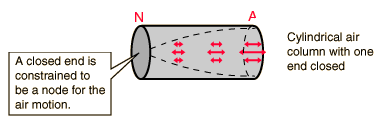
\includegraphics[]{closedpipe.png}
% \end{marginfigure}
% When any musical instrument is played the note you hear is at the fundamental frequency but a number of harmonics are also present.  The relative intensity of the different harmonics determines the quality of the note you hear.  It is this, which enables us to distinguish the same note played on different instruments.

% If the tube is open at both ends both ends have an antinode and the fundamental occurs when the tube length is half a wavelength.  Harmonics are at whole number multiples of the fundamental frequency. \begin{marginfigure}
% 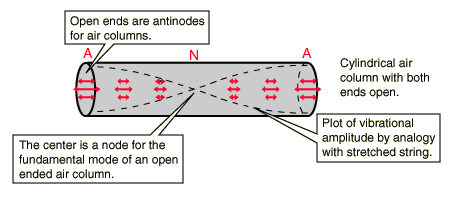
\includegraphics[]{openpipe.png}
% \end{marginfigure}

% \begin{figure}
% 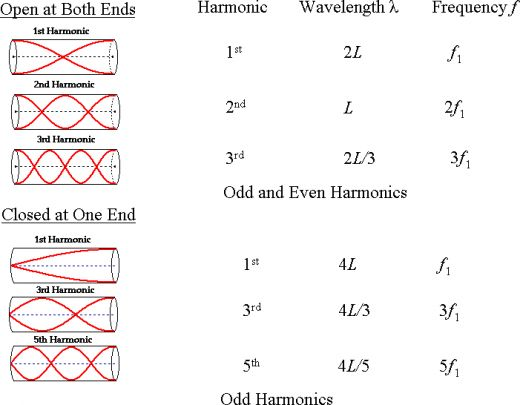
\includegraphics[]{pipes.jpg}
% \end{figure}
 
% \section{Refraction of Light}

% The Snell's Law equation is written in such a way as to emphasise symmetry. It is used to predict the change in direction that results from a change in velocity.\\
% \begin{figure*}
% \centering
% \begin{tikzpicture}[
%     media/.style={font={\footnotesize\sffamily}},
%     wave/.style={
%         decorate,decoration={snake,post length=1.4mm,amplitude=2mm,
%         segment length=2mm},thick},
%     interface/.style={
%         % The border decoration is a path replacing decorator. 
%         % For the interface style we want to draw the original path.
%         % The postaction option is therefore used to ensure that the
%         % border decoration is drawn *after* the original path.
%         postaction={draw,decorate,decoration={border,angle=-45,
%                     amplitude=0.3cm,segment length=2mm}}},
%    scale=1.2]
%     % Round rectangle
%     \fill[gray!10,rounded corners] (-4,-3) rectangle (4,0);
%     % Interface
%     \draw[blue,line width=.5pt,interface](-4,0)--(4,0);
%     % Vertical dashed line
%     \draw[dashed,gray](0,-3)--(0,3);
%     % Coordinates system
%     \draw(0,0.15)node[above]{$x$};
%     \draw[<->,line width=1pt] (1,0) node[above]{$y$}-|(0,-1) node[left]{$z$};
%     % Incidence
%     \draw[->,wave]
%          (150:4.5cm)--(150:3.5cm)node[right]{Incident ray};
%     \draw[gray](0:0cm)--(155:2cm);
%     \path (0,0)++(113:1cm)node{$\phi$};
%     \draw[->](0,0.75)arc(90:155:.75cm);
%     % Transmission
%     \draw[->,wave]
%          (-60:2.5cm)--(-60:3.5cm)node[right]{Refracted ray};
%     \draw[gray](0:0cm)--(-60:2cm);
%     \path (0,0)++(-70:1cm)node{$\theta$};
%     \draw[->] (0,-0.75) arc (-90:-60:.75cm);
  
%     % Media names
%     \path[media] (-3,.6)  node {media 1}
%                  (-3,-.6) node {media 2};

%     % $x$ axis
%     \filldraw[fill=white,line width=1pt](0,0)circle(.12cm);
%     \draw[line width=.6pt] (0,0)
%                           +(-135:.12cm) -- +(45:.12cm)
%                           +(-45:.12cm) -- +(135:.12cm);
%     % Interface pointer
%     \draw[-latex,thick](3.2,0.5)node[right]{$\mathsf{S_{1,2}}$}
%          to[out=180,in=90] (3,0);
         
%        \node at (0,-4){\begin{large}$\text{Snell's Law}=\frac{\sin\phi}{\sin\theta} = \frac{v_1}{v_2} = \frac{n_2}{n_1}$\end{large}};
%     % To-paths are really useful for drawing curved lines. The above
%     % to path is equal to:
%     %
%     % \draw[-latex,thick](3.2,0.5)node[right]{$\mathsf{S_{1,2}}$}
%     %      ..controls +(180:.2cm) and +(up:0.25cm) .. (3,0);
%     % Internally the to path is translated to a similar bezier curve,
%     % but the to path syntax hides the complexity from the user. 
% \end{tikzpicture}
% \caption{Refraction from low refractive index to higher refractive index (eg. Air to glass)}
% \end{figure*}
% Looking at the equation for snell's law we see that there must be a point at which the incident ray causes a refraction at, or above 90 degrees. This is called the \textbf{\textit{critical angle}}. At shallower angles of incidence, total internal reflection occurs.
% The only application of total internal reflection required to be learnt is the step-index multimode (`thick core') optical fibre. Step-index means simply that the core is glass of one refractive index and the cladding is glass of a lower index (students need to know why it has to be lower), with an abrupt change in index at the interface.
% \begin{figure*}
% \centering
% \begin{tikzpicture}[scale=1]
% \shade[left color=black!40!white,right color=black!10!white](0,-2.5)--(10,-2.5)--(10,2.5)--(0,2.5)--cycle;
% \draw[dashed, thin, red](-1,0)--(11,0);
% \draw[thin](0,-2.50)--(0,2.5);
% \draw(0,2)--(10,2);
% \draw(0,2.5)--(10,2.5);
% \draw(0,-2)--(10,-2);
% \draw(0,-2.5)--(10,-2.5);
% \draw[thick, blue,->](-1.8,-1)--(0,0)--(2,2)node(A){}--(6,-2)--(9.5,2);
% \draw[dashed, thin](2,1)--(2,3)node[]{};
% \node at (1,2.25){$n_2$};
% \node at (1,-1.75){$n_1$};
% \draw[->](2,1.4)arc(-90:-125:.75cm)node[anchor=north,midway]{$\theta_i$};
% \draw[->](2,2.75)arc(90:-40:.75cm)node[anchor=south,midway]{$\theta_r$};
% \node at (7,3.25){$n_1 \sin{\theta_i}=n_2 \sin{\theta_r}$};
% \node at (9,-1.75){\tiny Core};
% \node at (9,-2.35){\tiny Cladding};
% \begin{scope}
% \path[clip,decoration={random steps, segment length=6pt, amplitude=3pt},decorate] (9.9,-2.6)--(9.9,2.6)--(11,2.6)--(11,-2.6)-- cycle; 
% \shade[left color=white,right color=white](9.9,-3)--(9.9,3)--(11,3)--(11,-3)-- cycle;
% \end{scope}
% \end{tikzpicture}
% \caption{Total internal reflection in a single fibre}

% \end{figure*}
% While such fibres are fine for conveying light for illumination, students need to know that they can't be used for transmitting a rapid sequence of data over a long distance. Multimode dispersion is the problem.
% \begin{figure*}
% \centering
% \pgfmathdeclarefunction{gauss}{2}{%
%   \pgfmathparse{1/(#2*sqrt(2*pi))*exp(-((x-#1)^2)/(2*#2^2))}%
% }
% \begin{tikzpicture}[scale=1]

% \shade[left color=black!40!white,right color=black!10!white](0,-2.5)--(10,-2.5)--(10,2.5)--(0,2.5)--cycle;
% \draw[dashed, thin, red](-1,0)--(10,0);
% \draw[thin](0,-2.50)--(0,2.5);
% \draw(0,2)--(10,2);
% \draw(0,2.5)--(10,2.5);
% \draw(0,-2)--(10,-2);
% \draw(0,-2.5)--(10,-2.5);
% \draw[thick, blue,->](-1.8,-1)--(0,0)--(2,2)--(6,-2)--(9.5,2);
% \draw[thick, cyan,->](-2.2,-1)--(0,0)--(2.3,2)--(6.6,-2)--(10.9,2);
% \draw[dashed, thin](2,1)--(2,3)node[]{};
% \draw[dashed, thin](2.3,1)--(2.3,3)node[]{};
% \node at (1,2.25){$n_2$};
% \node at (1,-1.75){$n_1$};
% \node at (9,-1.75){\tiny Core};
% \node at (9,-2.35){\tiny Cladding};
% \node at (12,-3.25){\tiny{Broad pulse}};
% \node at (-3,-3.25){\tiny{Defined pulse}};
% \begin{scope}
% \path[clip,decoration={random steps, segment length=6pt, amplitude=3pt},decorate] (9.9,-2.6)--(9.9,2.6)--(11,2.6)--(11,-2.6)-- cycle; 
% \shade[left color=white,right color=white](9.9,-3)--(9.9,3)--(11,3)--(11,-3)-- cycle;
% \end{scope}

% \begin{axis}[scale=.5,
%     anchor=origin,
%     at={(-3cm,-3cm)},
%     style={samples=51,smooth},
%     hide axis
% ]
% \addplot[mark=none,thick] {gauss(0,.4)};
% \end{axis}
% \begin{axis}[scale=.5,
%     anchor=origin,
%     at={(12cm,-3cm)},
%     style={samples=51,smooth},
%     hide axis
% ]
% \addplot[mark=none,thick] {gauss(0,2)};
% \end{axis}

% \draw[thick, blue,->](-1.8,-1)--(0,0)--(2,2)--(6,-2)--(9.5,2);
% \draw[thick, cyan,->](-2.2,-1)--(0,0)--(2.3,2)--(6.6,-2)--(10.9,2);
% \end{tikzpicture}
% \caption{Multi-mode dispersion in a fibre resulting from the two different length paths}
% \end{figure*}

% Light travelling at an angle to the axis of the fibre will travel further for a given axial length of fibre, than light travelling parallel to, or at a smaller angle to, the axis, and so will arrive later. Thus the arrival time of an element of data encoded in the light is smeared out. The element could start to arrive (by the shortest route) earlier than the previous element has finsished arriving by its longest route. Even worse confusion can occur. 
% There are two ways round the problem of multimode dispersion\ldots
% \begin{itemize}
% \item Make fibres with graded index cores. This means cores which have a progressively lower index as we go out from the axis towards the interface with the cladding. The lower the index the faster the light travels so, if the grading is correctly calculated, the longer, more zigzaggy, paths cash in on the `faster medium' and take no longer than the short, axial, route. Clever stuff, but note that graded index fibres are not in the WJEC specification. 
% \item Make the core very thin. Its diameter must  be no more than a few wavelengths of the light (or infrared) being carried. Such fibres are monomode. Light travels parallel to the axis. There are no zigzag modes. Students are required to know this. You are not required to know why very thin fibres are monomode. This is just as well, because it cannot be shown by ray optics, nor even by simple application of Huygens Principle. Electromagnetic wave theory is needed.
% \end{itemize}
% The website\\ \url{http://www.techoptics.com/pages/Fiber\%20Optics\%20-\%20Optical\%20Fiber.html}   \\ 
% gives an excellent summary of fibres for data transmission, with some facts and figures.

% \section{Photons}

% Everything in nature seems to come in lumps or quanta (singular: quantum). For example, ordinary matter is made of atoms, and electric charge comes in units of e. This lumpiness was only becoming fully accepted a hundred years ago. But in 1905 Einstein made the bold suggestion that light, too, was `lumpy'. Light quanta are now called photons.
% A photon is a discrete packet of electromagnetic radiation energy. The energy of a photon is given by
% $$ E=hf $$
% In which $f$ is the frequency of the light and $h$ is a constant called Planck's constant. $h = 6.6 \times 10^{-34} \text{Js}$ \sidenote{For interest only \ldots The constant h had first arisen in the earlier (1900) work of Max Planck on the radiation inside a cavity with hot walls. Planck had shown that the energies of oscillating particles in the wall seemed to be quantised.}

% Einstein suggested some experiments in which the quantisation of light should reveal itself. The simplest to understand involved the photoelectric effect, a phenomenon known about since the late 1880s.

% \section{Laser Physics}
% Lasers, by now, are in nearly every household as they were once in every self-respecting science fiction film. Although, the death ray mystique will appeal to most A-level students there is real value in studying the physics which forms the foundation of laser construction. Unlike other subjects such as relativity or nuclear physics which can only be touched upon within an A-level course, the essential physics underpinning lasers can be taught reasonably well in a few lessons. Also, these fundamentals of lasers can be taught at the right level while not oversimplifying the subject.

% LASER is an acronym and stands for Light Amplification by Stimulated Emission of Radiation. Which leads us nicely onto what is stimulated emission?

% \subsection{The Three Important Atomic Processes}
% These three processes are:
% \begin{enumerate}
% \item Absorption of light
% \item Spontaneous emission of light
% \item Stimulated emission of light
% \end{enumerate}
% Absorption of light by an atom is shown in the diagram below - a photon of the correct energy is absorbed by the atom and an electron gains enough energy to move from the ground state to the excited state (Note: for the moment we are only considering the ground state and the first excited state only).

% \begin{figure*}
% \usetikzlibrary{shadings}
% \centering
% \begin{tikzpicture} [scale=.7, wave/.style={
%         decorate,decoration={snake,post length=1.4mm,amplitude=2mm,
%         segment length=2mm},thick},
%     interface/.style={
%         % The border decoration is a path replacing decorator. 
%         % For the interface style we want to draw the original path.
%         % The postaction option is therefore used to ensure that the
%         % border decoration is drawn *after* the original path.
%         postaction={draw,decorate,decoration={border,angle=-45,
%                     amplitude=0.3cm,segment length=5mm}}} ]
   
% \pgfdeclareverticalshading{rainbow}{100bp} 
%  {color(0bp)=(red); color(25bp)=(red); color(35bp)=(yellow); 
%   color(45bp)=(green); color(55bp)=(cyan); color(65bp)=(blue); 
%   color(75bp)=(violet); color(100bp)=(violet)}
%     \begin{scope}[]
%         \shade[shading=rainbow]
%             (0,0) rectangle (3,8); 
%     \draw[very thick,black] (0,3) -- (3,3);
%     \draw[very thick,black] (0,6.3) -- (3,6.3);
%      \end{scope}
% \draw[thick, black] (3.5,-1)--(10,-1);
% \draw[thick, black] (3.5,3)--(10,3);
% \draw[thick, black] (3.5,6.3)--(10,6.3);
% \draw[dashed,<-]  (5,6.3)--(5,-1);
% \draw[dashed,<-]  (7,3)--(7,-1);
% \draw[wave,blue,->](-2,8.5)--(5,3.5);
% \draw[wave,green,->](-1,6)--(7,1);
% \draw [fill=black] (5,-1) circle (2mm);
% \draw [fill=black] (7,-1) circle (2mm);
%     \end{tikzpicture}
%     \caption{Absorption of light. The photon energy has to correspond to a possible energy level transition for the energy to be absorbed by an electron.}
% \end{figure*}
 
% Spontaneous emission is the reverse process - an electron drops spontaneously (and randomly) from the excited state to the ground state and emits a photon of the same energy. These photons have random phase and random direction.

% \begin{figure*}
% \usetikzlibrary{shadings}
% \centering
% \begin{tikzpicture} [scale=.7, wave/.style={
%         decorate,decoration={snake,post length=1.4mm,amplitude=2mm,
%         segment length=2mm},thick},
%     interface/.style={
%         % The border decoration is a path replacing decorator. 
%         % For the interface style we want to draw the original path.
%         % The postaction option is therefore used to ensure that the
%         % border decoration is drawn *after* the original path.
%         postaction={draw,decorate,decoration={border,angle=-45,
%                     amplitude=0.3cm,segment length=5mm}}} ]
   
% \pgfdeclareverticalshading{rainbow}{100bp} 
%  {color(0bp)=(red); color(25bp)=(red); color(35bp)=(yellow); 
%   color(45bp)=(green); color(55bp)=(cyan); color(65bp)=(blue); 
%   color(75bp)=(violet); color(100bp)=(violet)}
%     \begin{scope}[]
%         \shade[shading=rainbow]
%             (0,0) rectangle (3,8); 
%     \draw[fill=black] (0,0) rectangle (3,3);
%     \draw[fill=black] (0,3.1)rectangle (3,5); 
% \draw[fill=black] (0,5.1)rectangle (3,8); \end{scope}
% \draw[thick, black] (3.5,0)--(10,0)node[anchor=west]{Ground State};
% \draw[thick, black] (3.5,3)--(10,3)node [anchor=west]{$2.32eV$};
% \draw[thick, black] (3.5,5)--(10,5) node [anchor=west] {$2.75eV$};
% \draw [fill=black] (5,5) circle (2mm);
% \draw [fill=black] (7,3) circle (2mm);
% \draw[dashed,->]  (5,5)--(5,0);
% \draw[dashed,->]  (7,3)--(7,0);
% \draw[wave,blue,->](5,2)--(8,2)node[anchor=west]{$\lambda=?$};
% \draw[wave,green,->](7,1)--(10,1)node[anchor=west]{$\lambda=?$};
 
%     \end{tikzpicture}
%     \caption{Emission spectra and corresponding energy levels. Note: the frequency and wavelength can be calculated from the change in energy of the electron using $E=hf$}
% \end{figure*}
% However, there is also a third process [which was originally proposed by Einstein in 1917]. This process is known as stimulated emission - an electron is `stimulated' to drop from its excited state by an incoming photon. 


% \begin{figure}
% 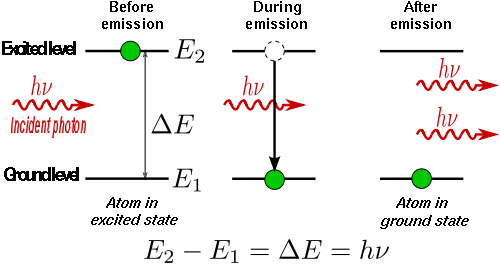
\includegraphics[scale=.5]{stimem.png}
% \caption{Stimulated emission - an incoming photon of an energy matching the transition can cause an electron to drop to a lower energy level. In order to do this it must release a photon identical to the first.}
% \end{figure}


% The reason that the electron is stimulated to drop is that the incoming photon is an electromagnetic wave and its e-m field will exert an oscillating force on the excited electron. If the incoming photon is of the correct frequency, this oscillating force will cause the excited electron to drop and both photons will exit with the same frequency, phase and direction. Note: again, the incoming photon needs to be of the correct energy.

% \subsection{Inverting The Population}
% In order to get as much light out of a system as is possible we need to get as many atoms excited as is possible.\begin{marginfigure}
% 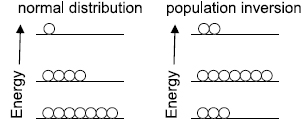
\includegraphics[]{popin.jpg}
% \caption{Population inversion - when more electrons are in an excited state than in the ground state. This is the opposite of a `normal' situation}
% \end{marginfigure} Obviously, the more electrons we have in an excited state the more will drop and emit photons (either spontaneously or through stimulation). However, there is one serious problem that arises when we produce a lot of light - the very photons that we produce are the actual photons that can be absorbed (they have the correct energy to produce both effects). If we have photons being absorbed all the time then our laser beam isn't getting any stronger.

% Forget, for the moment about spontaneous emission (we are allowed to but we'll explain why later). When a photon arrives at an atom one of three things can happen:
% \begin{enumerate}
% \item It can pass by and do nothing.
% \item It can be absorbed (if the atom is in the ground state).
% \item It can cause stimulated emission (if the atom is in the excited state).
%  \end{enumerate}
% When it comes to producing a laser beam with a high intensity the three options above will have the following effect on the beam.
% \begin{enumerate}
% \item No change in the beam.
% \item Net loss of one photon from the beam.
% \item Net gain of one photon in the beam.
% \end{enumerate}
% We need to arrive at a situation where stimulated emission is more likely than absorption so that the laser beam increases in intensity. Since stimulated emission occurs if the electrons are in the upper level and absorption when electrons are in the lower level we need to get more electrons into the upper, excited level. This is called population inversion (or $N_{2} > N_{1}$ as stated in the syllabus, where $N_2$ and $N_1$ are the number of electrons in the excited state and the ground state respectively).

% Unfortunately, this goes against what happens in nature - lower energy levels are always more heavily populated than higher energy levels when we have thermal equilibrium. There's only one thing for it - get rid of this thermal equilibrium. How do we do this? We continue to pump energy into exciting electrons to higher energy levels to maintain a population inversion and to break the conditions of thermal equilibrium.

% Population inversion is not usually possible if we only have two energy levels (if pumping is carried out by light).
%  \newpage
% \subsection{The 3 Energy Level Laser System}

% \begin{figure}
% 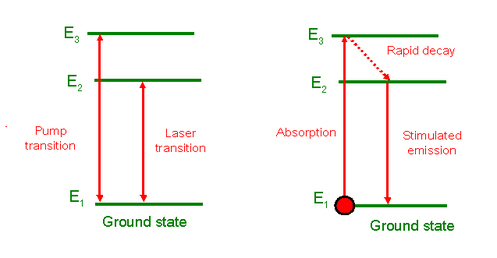
\includegraphics[]{lasers.jpg}
% \end{figure}
% \sidenote{Note:\begin{itemize} \item E3 (to E2) has to have a short lifetime because E3 cannot start to fill up - pumping won't then be possible. Also, we don't want the electrons to stay in E3 and have them stimulated to drop back to E1 by the pumping light - that's back to the 2-level system again which wasn't quite good enough.

% \item More than half the electrons from E1 must be pumped to E2 (via E3) in order to obtain a population inversion - that's a lot of electrons!\end{itemize}}
% \begin{enumerate}
% \item Pumping. Electrons are promoted from the ground state (E1) to E3 usually by using an external light source or by electron collisions.
% \item Electrons drop quickly (because E3 is chosen to have a short lifetime of the order of nanoseconds) to the metastable (E2). Calling E2 metastable means that it has a long lifetime and electrons stay there for a long time (not that long really around a millisecond but that's a very long time for an electron).
% \item This is the transition that produces the laser photons so we must have N2 > N1. Note that, although stimulated emission still reduces our population inversion, the pumping is at a different wavelength. We have to make sure that the pumping [1] exceeds the stimulated emission [3] to maintain a population inversion.
% \end{enumerate}

% \subsection{The 4 Energy Level Laser System}

% \begin{figure*}
% 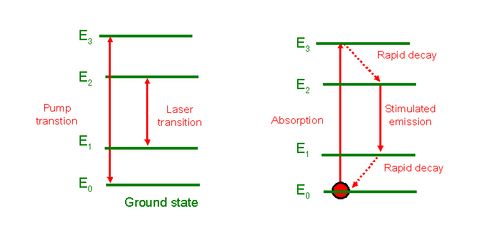
\includegraphics[]{fourlevel.jpg}
% \end{figure*}
% \begin{enumerate}
% \item Pumping again.
% \item Quick drop to the metastable state E2.
% \item This is the laser light producing transition so this time N2 > N1. However, because E0 is the ground state, E1 is practically empty initially so obtaining population inversion is far, far easier (definitely no need to pump half the electrons!).
% \item Another quick transition so E1 has a short lifetime. This is because we want E1 to be empty so that we have a population inversion (if N1 is small it's easier for N2 to be larger than N1).							
%  \end{enumerate}
% \subsection{Laser Construction}

% \begin{figure*}
% 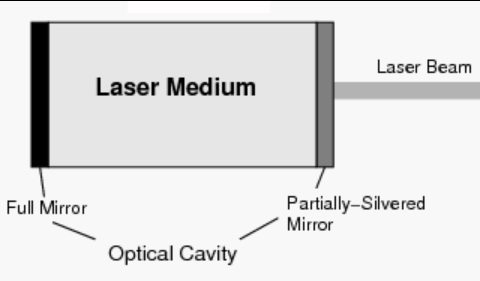
\includegraphics[scale=.5]{lasercav.PNG}
% \end{figure*}

% In order to ensure that the laser produces light of a high enough intensity, the above set up is used. The amplifying medium is the region where the population inversion exists. This means that the conditions are right in the amplifying medium for stimulated emission. Under these conditions one photon has the potential to produce two photons and these can produce 4 photons, then 8 photons etc. Like a chain reaction, this process will lead to an exponential increase in output energy. Laser physicists aren't happy with this, they go even further - they use mirrors to ensure that this exponential increase happens many times. Because only 1\% of the light exits each time it reflects back and forth between the mirrors, on average, the beam will pass through the amplifying medium a hundred times before it exits. Now, considering that each time the beam passes through the amplifying medium it is increasing exponentially, this factor of 100 makes an enormous difference. 

% This all leads to very high light intensities inside the amplifying medium and this is why (as was said earlier) we can forget about spontaneous emission. Imagine that you're an excited electron sitting happily in your higher energy level. Normally, you'll just drop down spontaneously when your time is up. But, inside a laser, there's so much light that you never drop spontaneously because before your time's up you've been disturbed by another photon, stimulated to join in with all the other light and join in coherently as well!

% \subsection{Efficiency}
% Usually, lasers are very inefficient beasts. Because of the large energies required to maintain a population inversion, their efficiencies are generally far below 1\%. Some reasons for this:
% \begin{itemize}
% \item The pumping energy is considerably larger than the output photon energy.
% \item High intensity pumping combined with the high intensity of the laser beam means that the amplifying medium will get very hot. So, there will be large heat losses. To make this matter worse, we need to cool the amplifying medium usually so that it, or its container, doesn't melt. By cooling the system we just transfer more heat and increase our losses but better this than destroy a \textsterling 50 000 laser!
% \end{itemize}
 
% \subsection{Semiconductor Lasers}
% The basic structure of a standard `edge emitting' semiconductor laser is shown below. The whole block shown below is a semiconductor chip with dimensions approximately 0.5mm $\times$ 0.5 mm $\times$ 1 mm.
% \begin{figure*}
% 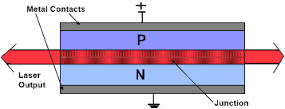
\includegraphics[]{diode.png}
% \end{figure*}

 
% The above laser fits the basic shape of a normal laser, the mirrors, however, are far from the 100\% and 99\% reflecting ideals discussed earlier. The mirrors are simply due to the semiconductor-air boundary at the edges of the chip. [This in fact gives 40\% reflection only (at both sides).] This would be disastrous for highly inefficient gas lasers but not for our semiconductor laser. The reason why:
% \begin{itemize}
% \item The population inversion inside the semiconductor sandwich area is millions of times higher than in gas lasers [$10^{25}$ electrons/$m^{3}$].
% \item The exponential increase in light intensity (i.e. 1 photon becoming two, becoming four etc.) occurs far more quickly because of the higher population inversion.
% \item So the fact that we lose 60\% of the light at each reflection is compensated for by having huge gains between the mirrors.
%  \end{itemize}

% \subsection{Advantages and Uses of Laser Diodes}
% These are straightforward and can be summarised as follows:

% Advantages:
% \begin{itemize}
% \item Cheaper
% \item Smaller
% \item More efficient
% \item Easy to mass produce	
% \end{itemize}
% Some uses:
% \begin{itemize}
% \item Inside DVD and CD players
% \item Bar-code readers
% \item Telecommunications (via optical fibres)
% \item Image scanning
% \item Laser surgery
% \end{itemize}
% The usefulness of laser diodes is `reflected' in the number of them produced annually - around 1 billion (109) laser diodes are produced worldwide per year!
 
% For more than enough further reading see:
% \begin{itemize}
% \item \url{http://members.aol.com/WSRNet/tut/ut1.htm}
% \item Wikipedia \url{http://en.wikipedia.org}  then type `laser' or `semiconductor laser'
% \item Google search `laser theory'
% \end{itemize}


	
\subsection{End-of-chapter questions}



\subsection*{Wave terminologies}

\question{
	A bottle floating on a water surface is seen to bob up and down over a distance of 20 cm twice each second. What is its amplitude and its frequency?
}

\question{A horn produces a note of frequency of 512 Hz. Given that sound travels at $330 \mps$ in air, find the wavelength of this sound wave.}

\begin{marginfigure}
	\vspace*{-12pt}
	\centering
	\begin{tikzpicture}[scale=0.78]
	\draw[help lines, gray!50, very thin, step=0.2] (0,-2) grid (6,2);
	\draw[help lines, step=1] (0,-2) grid (6,2);
	\foreach \y in {-2,-1,0,1,2} \node[left] at (0,\y) {$\y$};
	\foreach \x in {0,0.1,0.2,0.3,0.4,0.5,0.6} \node[below] at (10*\x,-2) {$\x$};
	\node at (-1.2,1.5) {$y$/cm};
	\node at (5,-2.8) {$x$/m};
	\draw [thick, blue, domain=0:6, samples=30, smooth] plot (\x,{1.6*sin(75*\x)});
	\draw [thick, Green, domain=0:6, samples=30, smooth] plot (\x,{-0.8*cos(120*\x)});
	\node[blue] at (1.8, 1.6) {$P$};
	\node[Green] at (4.5, 1.1) {$Q$};
	\end{tikzpicture}
	\vspace*{-18pt}
\end{marginfigure}

\question{The graph shows the variation of displacement $y$ with the distance $x$ of wave $P$ and wave $Q$ at some instant. (a) For each of the two waves, state the amplitude and the wavelength. (b) Given that both waves have a time period of 0.30 s, find the frequency of the waves, and hence find the speed for each wave.}


\subsection*{transverse \& longitudinal waves}

\question{
	An ultrasound waves of frequency 2.0 MHz travels with a speed of $1600 \mps$ through water. What is the shortest distance from a point of maximum pressure to a point of	minimum pressure?
}

\begin{marginfigure}
	\vspace*{-12pt}
	\centering
	\begin{tikzpicture}[xscale=0.6,yscale=0.75]
	\draw [->] (0,-2) -- (0,2.4) node[midway,left]{$O$} node[left]{$y$};
	\draw [->] (0,0) -- (2.5*pi,0) node[below]{$x$};
	\draw[very thick,->] (1.6*pi,2) -- (2.4*pi,2);
	\node[above,twoline] at (2*pi, 2.2) {direction of\\wave motion};
	\draw [thick, blue, domain=0:2.4*pi, samples=30, smooth] plot (\x,{1.6*sin(\x*1.2 r)});
	\draw[fill, red] (5*pi/12,1.6) circle (0.08) node[above, black]{$P$};
	\draw[fill, red] (10*pi/12,0) circle (0.08) node[above right, black]{$Q$};
	\draw[fill, red] (15*pi/12,-1.6) circle (0.08) node[below, black]{$R$};
	\draw[fill, red] (20*pi/12,0) circle (0.08) node[above left, black]{$S$};
	\end{tikzpicture}
	\vspace*{-16pt}
\end{marginfigure}

\question{
	The graph shows the variation with distance $x$ of the displacement $y$ of a wave on a stretched rope at
	time $t = 0$. The wave has a frequency of 1.0 Hz. (a) State and explain whether this wave is transverse or longitudinal. (b) For the points $P$, $Q$, $R$, and $S$ labelled on the graph, which one of them is moving upwards with greatest speed at $t=0$? (c) Sketch the wave pattern at $t = 0.50 \text{ s}$. (c) For the points $P$, $Q$, $R$, and $S$, what are their positions at $t = 0.50 \text{ s}$?
}


\question{
	Given a slinky toy, suggest how you can demonstrate (a) a transverse wave, (b) a longitudinal wave to your classmates.
}

\subsection*{Sound waves}

\question{
	If some alien civilisation blows up the moon one day, can we hear it?
}

\question{An oscilloscope is used to measure a sound wave. When the time base is set at 5.0 ms div$^{-1}$, 3 complete waveforms are observed over 5 divisions. Calculate, (a) the period of the wave, (b) the frequency of the wave.}

\question{Describe the changes to the wave pattern displayed on an oscilloscope if the sound being measured has (a) a higher pitch, (b) a greater volume.}


\subsection*{Electromagnetic waves}

\question{
	Green light has a wavelength of 500 nm in vacuum. What is its frequency?
}

\question{
	An electromagnetic wave has a period of 1.0 ps. (a) What is the wavelength of this wave? (b) What is the number of wavelengths in a distance of 1.0 m?
}

\question{
	(a) What is the frequency of the longest-wavelength ultraviolet wave? (b) What is the frequency of the shortest-wavelength infra-red radiation?
}

\question{
	State a typical value for the wavelength for the following radiation in vacuum: (a) infra-red, (b) X-ray, (c) microwave, (d) ultraviolet.
}

\question{
	A student argues that the speed of an electromagnetic wave is proportional to its frequency because we have $c=\lambda f$. State and explain whether the student's argument is correct.
}

\question{
	(a) Suggest as many properties of electromagnetic waves as you can. (b) Among these properties you have listed, which property of electromagnetic wave is distinct from other transverse waves?
}

%\question{
%	Suppose a sound wave and an electromagnetic wave have the same wavelength, compare their frequencies.
%}

\subsection*{Intensity of waves}

\question{
	A sound wave in air has an amplitude $A_0$ and intensity $I_0$. If the amplitude increases to $3A_0$, what is the new intensity?
}

\question{
	The intensity of radiation arriving normally on a solar panel was $500 \text{ W m}^{-2}$. (a) If the panel has an effective area of $4.0 \text{ m}^2$, how much energy would arrive in one hour? (b) If the radiation has double the amplitude, how much energy would arrive in one hour?
}

\question{
	The intensity $I$ of a sound wave can be given by the formula: $I = k v \rho f^2 A^2$, where $v$ is the speed of sound, $\rho$ is the density of the medium, $f$ is the frequency and $A$ is the amplitude. Show that $k$ is a unit-free constant.
}



\question{
	A point source gives out spherical waves. How does the wave amplitude $A$ vary with the distance $r$ from the source?
}

\subsection*{Polarisation}

\question{
	A horizontally polarised beam of light of intensity $I_0$ passes through a polarising filter whose plane of polarisation is at $30^\circ$ to the horizontal. What is the transmitted intensity?
}

\question{
	When polarized light is sent through some chemical solution, the plane of polarization is rotated. If the intensity is $I$ without the solution being placed in the beam but $0.80I$ after the sugar is placed in the beam, what is the angle of rotation?
}

\question{
	A beam of unpolarised light is sent through two polarising filters $A$ and $B$. Filter $A$ has its axis of
	polarisation in the vertical direction, and filter $B$ has its axis of polarisation in the horizontal direction. (a) What is the emergent intensity? (b) A third polarising filter $C$ is inserted between the filters $A$ and $B$, such that filter $C$ has its plane of polarisation at an angle of $45^\circ$ to the vertical. What is the new emergent intensity?
}

\question{
	Suggest how you may use a stretched elastic rope to demonstrate the phenomenon of polarisation.
}

\subsection*{Diffraction}

\question{
	A hill stands between a house and a radio transmitter, but radio signals sent from the transmitter are still received at the house. How can this happen?
}

\question{
	Diffraction can be demonstrated by observing how water waves in a ripple tank go through a gap. Suggest whether the following action would lead to greater or less obvious diffraction: (a) increasing the frequency of the water waves, (b) increasing the amplitude of the waves, (c) increasing the width of the gap, (d) increasing the speed of the waves by increasing the depth of water.
}

\question{
	Microwave ovens use microwaves of frequency of around 2.4 GHz to heat food. The front door of many microwave ovens is made of glass with a metal grid, where gap in the grid are a few mm across. By reference to the wavelength of the microwave, explain how the front door keeps microwaves in but could let light out.
}

\subsection*{Doppler effect}

For the questions below, take the speed of sound to be $340 \mps$. 

\question{A car travels with a constant speed along a straight road. The car's horn is known to sound at a frequency of 500 Hz, but an observer standing on the roadside hears a frequency of 450 Hz. What is the magnitude and the direction of the car's velocity relative to the observer?}


\question{
	An ambulance travelling at a steady speed of $25 \mps$ passes close to a stationary observer. The warning signal on the ambulance has a frequency of 1500 Hz. What is the overall change in the frequency heard by the observer as the ambulance goes by?
}

\question{
	If the motion of the source is at right angles to an observer, state and explain whether there will be a Doppler effect?
}


\question{
	A girl sits on a horizontal platform that is rotating about a vertical axis. The girl moves in a circular path with a constant speed of $8.0 \mps$. The girls starts blowing a whistle which emits a sound of frequency 1200 Hz. To an observer standing at a distance, (a) find the maximum and the minimum frequency heard. (b) Describe the variation in the frequency of the sound heard by the observer.
}

\question{
	A spectral line of a particular wavelength is emitted from a distant star. The wavelength observed is found to vary periodically from a maximum value to a minimum value and back to the maximum value. What can you say about the motion of the star?
}



\question{
	[This question is beyond CAIE syllabus] (a) A source emits sound wave of frequency $f$. If the observer, rather than the source, is in motion, suggest whether there is any change in the apparent frequency $f^\prime$ heard by the observer. (b) If the observer is moving towards the source at a velocity of $v_o$, show that the observed frequency $f'$ is: $f' = f \frac{v+v_o}{v}$. (c) If the observer is moving away from the source, derive a similar expression for the observed frequency. 
}

\section{Superposition of Waves}

When two of more waves meet together, the resultant motion is a combination of the individuals. They can form a \emph{resultant wave} when they overlap, after which they cross one another and neither is affected. In this chapter, we will study the principle of superposition, and look at two important consequences: the phenomenon of \emph{interference} and \emph{stationary waves}.

\subsection{Superposition of waves}



\subsection{Principle of superposition}

\begin{ilight}
	 When two (or more) waves meet to form a resultant wave, the \keypoint{principle of superposition} states that the resultant displacement is the vector sum of each individual displacement\index{superposition of waves!principle of superposition}
\end{ilight}

\example{Displacement–time graphs for two waves $A$ and $B$ meeting at some point, together with the resultant wave formed at that point.}

\begin{figure*}[ht]
	\centering
	\begin{minipage}{0.45\textwidth}
		\centering
		\begin{tikzpicture}[scale=0.8]
		\draw [->] (0,-2) -- (0,2) node[above]{displacement};
		\draw [->] (0,0) -- (6.4,0) node[below]{$t$};
		\draw [Green, dashed] (0,0) --++ (0.8,1) --++ (1.6, -2) --++ (1.6,2) --++ (1.6, -2) --++ (0.4,0.5) node[below right]{$A$};
		\draw [purple, dashed] (0,-0.8) -- (1.6,-0.8) -- (2.4, 0.4) -- (4 ,0.4) -- (4.8, -0.5) -- (5.6, -0.5) -- (6, 0.4) node[right]{$B$}; 
		\draw [thick, blue] (0,-0.8) -- (0.8, 0.3) -- (1.6, -0.8) -- (2.4, -0.6) -- (4, 1.4) -- (4.8, -0.5) -- (5.6, -1.5) -- (6,0.1);
		\end{tikzpicture}
	\end{minipage}\hfil
	\begin{minipage}{0.45\textwidth}
		\centering
		\begin{tikzpicture}[scale=0.8]
		\draw [->] (0,-2) -- (0,2) node[above]{displacement};
		\draw [->] (0,0) -- (6.4,0) node[below]{$t$};
		\draw [Green,dashed,domain=0:6,samples=30,smooth] plot (\x,{0.6*sin(\x*3 r)}) node[below right]{$A$};
		\draw [purple,dashed,domain=0:6,samples=30,smooth] plot (\x,{1.2*sin(\x*1.5 r)}) node[above right]{$B$};
		\draw [thick,blue,domain=0:6,samples=30,smooth] plot (\x,{1.2*sin(\x*1.5 r) + 0.6*sin(\x*3 r)});
		\end{tikzpicture}
	\end{minipage}
\end{figure*}

Two important situations are constructive superposition and destructive superposition\index{superposition of waves!constructive superposition}\index{superposition of waves!destructive superposition}

\keypoint{Constructive superposition} occurs when resultant wave has greatest possible amplitude. This happens when peaks of the two waves meet together (also trough meets trough)\footnote{This statement is implicitly for transverse waves. For longitudinal waves to superpose constructively, the regions of compression (or rarefaction) must overlap.} 	peaks of both waves must arrive with a time difference $\Delta t = 0, \, T, \, 2T, \cdots$
	
\keypoint{Destructive superposition} occurs when amplitudes of each wave cancel out one another this happens when peak of one wave overlaps with trough of the other wave peaks of both waves must arrive with a time difference $\Delta t = \frac{1}{2}T, \, \frac{3}{2}T, \, \frac{5}{2}T, \cdots$

\begin{figure*}[ht]
	\centering
	\noindent\begin{minipage}{0.45\linewidth}
		\centering
		\begin{tikzpicture}[xscale=0.8, yscale=0.75]
		\draw [->] (0,-2) -- (0,2) node[above]{displacement};
		\draw [->] (0,0) -- (6.4,0) node[below]{$t$};
		\draw [Green, dashed,domain=0:6,samples=30,smooth] plot (\x,{0.6*sin(\x*1.2 r)});
		\draw [purple, dashed,domain=0:6,samples=30,smooth] plot (\x,{1.2*sin(\x*1.2 r)});
		\draw [thick,blue,domain=0:6,samples=30,smooth,variable=\x] plot (\x,{1.8*sin(\x*1.2 r)});
		\end{tikzpicture}
	\end{minipage}\hfil
	\begin{minipage}{0.45\linewidth}
		\centering
		\begin{tikzpicture}[xscale=0.8, yscale=0.75]
		\draw [->] (0,-2) -- (0,2) node[above]{displacement};
		\draw [->] (0,0) -- (6.4,0) node[below]{$t$};
		\draw [Green,dashed,domain=0:6,samples=30,smooth] plot (\x,{-1.2*sin(\x*1.2 r)});
		\draw [purple ,dashed,domain=0:6,samples=30,smooth] plot (\x,{1.6*sin(\x*1.2 r)});
		\draw [very thick,blue,domain=0:6,samples=30,smooth] plot (\x,{0.4*sin(\x*1.2 r)});
		\end{tikzpicture}
	\end{minipage}\hfil
	\caption{constructive and destructive superposition of two transvers waves}
\end{figure*}
\vspace{2cm}
Note: longitudinal waves are often represented by transverse diagrams. Transverse are much clearer and easier to read:
\vspace{1cm}
 

\begin{figure*}[htp]
	\centering
	\noindent\begin{minipage}{0.5\linewidth}
		\centering
		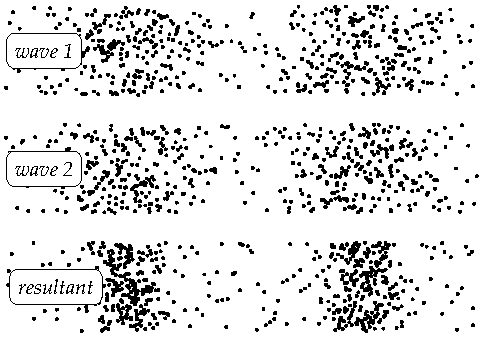
\includegraphics[width=.95\textwidth]{longitudinal+I.pdf}
	\end{minipage}\hfil
	\begin{minipage}{0.5\linewidth}
		\centering
		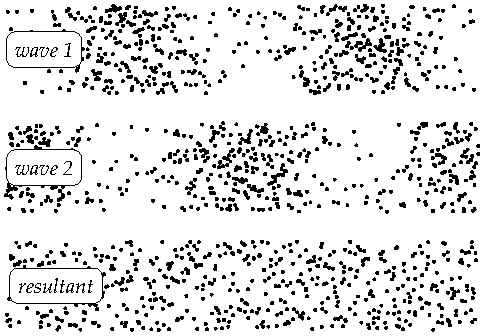
\includegraphics[width=.95\textwidth]{longitudinal-I.pdf}
	\end{minipage}
	\caption{constructive and destructive superposition of two sound waves} 
\end{figure*}


\subsection{Path difference}

The \keypoint{path difference}\index{path difference} is the difference in distance that two waves must travel from their sources to a given point. It plays a crucial role in wave interference, where waves can either constructively or destructively superpose depending on their path difference. Path difference is generally expressed in multiples of wavelength. To tell whether two waves superpose constructively or destructively:

{

\centering
\vspace*{6pt}
\begin{tcolorbox}[colframe=red, colback=yellow!30, width=0.65\textwidth]
	\setlength{\baselineskip}{\baselineskip}%
	
	\centering
	
	if ${\Delta L = 0, \, \lambda, \, 2\lambda, \cdots}$, then superposition is constructive
	
	if ${\Delta L = \frac{\lambda}{2}, \, \frac{3\lambda}{2}, \, \frac{5\lambda}{2}, \cdots}$, then superposition is destructive
	
\end{tcolorbox}\vspace*{-4pt}

}

\newpage

\example{Two loudspeakers are wired to produce identical sound signals in unison. The sound wave produced has a wavelength of 80 cm. Describe the volume you hear when you are at a distance of (a) 10 m from both speakers, (b) 10 m from one speaker and 12 m from the other?}

\begin{soln} path difference for case (a): $\Delta L = 10 - 10  = 0$

so constructive superposition, resultant amplitude is large, a loud sound is heard

path difference for case (b): $\Delta L = 12 - 10 = 2.0 \text{ m} \RA \Delta L = \frac{5}{2}\lambda$

so destructive superposition, resultant amplitude is small, sound is quiet \end{soln}

\subsection{Phase difference}

When two waves or two vibrating particles are compared, it is also useful to describe how much one is out of step with the other in terms of their \keypoint{phase difference}\index{phase difference} ($\Delta \phi$)
\footnote{More logically, we should first define the notion of \emph{phase angle} before talking about the \emph{phase difference}, which is simply the difference between the phase angles of two waves.
	
	Wave motion can generally be described by sine (or cosine) functions. Since the initial displacement of a wave is not necessarily zero, one can introduce a constant term that appears in the argument of the sine function. This term shifts the origin of the sine, and we call that the \emph{phase angle} $\phi$ of the wave, measured in radians (or degrees). One can think of $\phi$ as a number giving the fraction in a complete oscillation.
	
	In particular, the displacement $y$ of a transverse wave along the direction $x$ of energy transfer can be given by: $y = A \sin\left( \frac{2\pi x}{\lambda} - \frac{2\pi t}{T} + \phi \right)$. You can verify that this indeed describes a sinusoidal wave of wavelength $\lambda$ and period $T$ travelling at speed $v = \frac{\lambda}{T}$, while $\phi$ determines when and where the peaks show up.}

Phase difference is measured in radians (rad) or degrees ($^\circ$),  if two waves have a phase difference $\Delta \phi = 0,2\pi,4\pi,\cdots$, the two waves are said to be \keypoint{in phase}\footnote{If $\Delta \phi$ is given in degrees, then two waves are in phase if $\Delta \phi = 0, \, 360^\circ, \, 720^\circ, \cdots$}. In this case, peak of one wave overlaps with peak of the other. If two waves are not in phase, then they are said to be \keypoint{out of phase}
If $\Delta \phi = \pi, 3\pi, 5\pi, \cdots$, then two waves are completely out of phase, or \keypoint{anti-phase}\footnote{If $\Delta \phi$ is given in degrees, then two waves are anti-phase if $\Delta \phi = 180^\circ, \, 540^\circ, \, 900^\circ, \cdots$} in this case, peak of one wave meets the trough of the other. 

We can tell whether two waves superpose constructively or destructively from their phase difference as follows:

{
	
	\centering
	\vspace*{6pt}
	\begin{tcolorbox}[colframe=red, colback=yellow!30, width=0.65\textwidth]
		\setlength{\baselineskip}{\baselineskip}%
		
		\centering
		
		if ${\Delta \phi = 0, \, 2\pi, \,4\pi, \cdots}$, then superposition is constructive
		
		if ${\Delta \phi = \pi, \, 3\pi, \, 5\pi, \cdots}$, then superposition is destructive
		
	\end{tcolorbox}\vspace*{-4pt}
	
}






\newpage

Phase difference can also be related to path difference by: \begin{empheq}[box=\tcbhighmath]{equation*}{ \frac{\Delta \phi}{2\pi} = \frac{\Delta L}{\lambda} = \frac{\Delta t}{T} } \end{empheq}

\example{The diagrams below each shows the displacement of a particular point in two transverse waves. If both waves are travelling in the same direction with a wavelength of 30 cm, what is the phase difference and path difference between each wave?}

\begin{figure*}[htp]
	\centering
	\begin{minipage}{0.32\textwidth}
		\centering
		\begin{tikzpicture}[xscale=0.56,yscale=0.6]
		\draw [thick, ->] (0,0) --(7.5,0) node[below]{$t$};
		\draw [thick, ->] (0,-3) --(0,2.5) node[left]{$x$};
		\draw [thick,blue,domain=0:7,smooth] plot (\x,{2*sin(\x r)}) node[right]{$B$};
		\draw [thick,Green,domain=0:7,smooth] plot (\x,{2*sin(((\x - pi/2) r)}) node[right]{$A$};
		\end{tikzpicture}
		
		(a)
	\end{minipage}
	\begin{minipage}{0.32\textwidth}
		\centering
		\begin{tikzpicture}[xscale=0.56,yscale=0.6]
		\draw [thick, ->] (0,0) --(7.5,0) node[below]{$t$};
		\draw [thick, ->] (0,-3) --(0,2.5) node[left]{$x$};
		\draw [thick,blue,domain=0:7,smooth] plot (\x,{2*sin(\x r)}) node[right]{$B$};
		\draw [thick,Green,domain=0:7,smooth] plot (\x,{2*sin(((\x - pi) r)}) node[right]{$A$};
		\end{tikzpicture}
		
		(b)
	\end{minipage}
	\begin{minipage}{0.32\textwidth}
		\centering
		\begin{tikzpicture}[xscale=0.56,yscale=0.6]
		\draw [thick, ->] (0,0) --(7.5,0) node[below]{$t$};
		\draw [thick, ->] (0,-3) --(0,2.5) node[left]{$x$};
		\draw [thick,blue,domain=0:7,smooth] plot (\x,{2*sin(\x r)}) node[right]{$B$};
		\draw [thick,Green,domain=0:7,smooth] plot (\x,{2*sin(((\x - pi/3) r)}) node[below right]{$A$};
		\end{tikzpicture}
		
		(c)
	\end{minipage}
	\caption{examples of phases differences between two waves}
\end{figure*}

\begin{soln}
(a) $\Delta t = \frac{1}{4}T \RA \Delta \phi = \frac{1}{4}\times 2\pi = \frac{1}{2}\pi, \quad \Delta L = \frac{1}{4} \lambda = \frac{1}{4}\times30 = 7.5 \text{ cm}$

\eqyskip (b) $\Delta t = \frac{1}{2}T \RA \Delta \phi = \frac{1}{2}\times 2\pi = \pi, \quad \Delta L = \frac{1}{2} \lambda = \frac{1}{2}\times30 = 15 \text{ cm}$

\eqyskip (c) $\Delta t = \frac{1}{6}T \RA \Delta \phi = \frac{1}{6}\times 2\pi = \frac{1}{3}\pi, \quad \Delta L = \frac{1}{6} \lambda = \frac{1}{6}\times30 = 5.0 \text{ cm}$ \end{soln}


\subsection*{Brief summary}

The conditions for constructive and destructive superposition can be summarised as follows:

\begin{center}
{\renewcommand{\arraystretch}{1.25}
\begin{tabular}{|c|c|c|}
	\hline
	& constructive superposition & destructive superposition \\
	\hline
	simple criteria & peak meets peak & peak meets trough \\
	\hline
	time difference & $\Delta t = n \cdot T$ & $\Delta t = \left(n+\frac{1}{2}\right) \cdot T$ \\
	\hline
	path difference & $\Delta L = n \cdot \lambda$ & $\Delta L = \left(n+\frac{1}{2}\right) \cdot \lambda$ \\
	\hline
	phase difference & $\Delta \phi = n\cdot 2\pi\,$ or $\,n\cdot 360^\circ$ & $\Delta \phi = \left(n+\frac{1}{2}\right)\cdot 2\pi \,$ or $\,\left(n+\frac{1}{2}\right)\cdot 360^\circ$ \\
	\hline
\end{tabular}
}
\end{center}

where $n$ is a whole number: $n=0, 1, 2, 3 \cdots$

Remember that $\Delta t$, $\Delta L$ and $\Delta \phi$ are just different ways to describe how much one wave is ahead of/lag behind another wave, so they must be closely interrelated to each other.




\newpage

\subsection{Interference}

When two (or more) waves of constant phase difference meet, stable regions of constructive and destructive superposition are produced alternately, this phenomenon is called \keypoint{interference}\index{interference}



\begin{figure*}[htp]
	\centering
	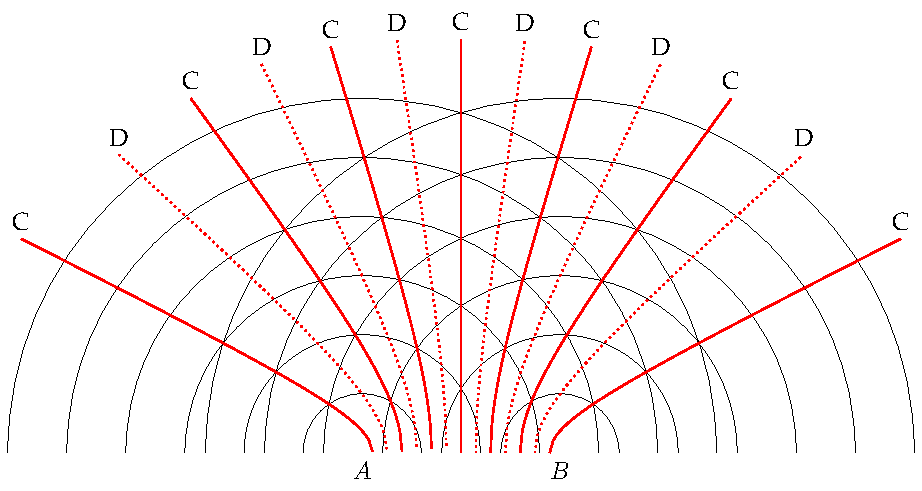
\includegraphics[width=1\textwidth]{interference.pdf}
\caption{constructive (solid lines) and destructive (dashed lines) interference of waves produced from two coherent sources $A$ and $B$}
\end{figure*}
\vspace{1cm}
Regions of constructive interference are often called \emph{maxima}

\begin{compactitem}
	\item[--] points on line C$_0$ are of equal distance to wave sources, i.e., path difference $\Delta L = 0$
	
	so maxima are observed along C$_0$
	
	\item[--] points on C$_1$, C$_2$ and C$_3$ have path difference $\Delta L = \lambda, \, 2\lambda, \, 3\lambda$
	
	so maxima are also formed along C$_1$, C$_2$ and C$_3$
	
	\item[--] equivalently, points on C$_n$ have phase difference $\Delta \phi = n\cdot 2\pi$, where $n=0,1,2,3,\cdots$
\end{compactitem} 

Regions of destructive interference are often called \emph{minima}

\begin{compactitem}
	\item[--] points on D$_1$, D$_2$ and D$_3$ have path difference $\Delta L = \frac{1}{2}\lambda, \, \frac{3}{2}\lambda, \, \frac{5}{2}\lambda$
	
	so maxima are also formed along D$_1$, D$_2$ and D$_3$
	
	\item[--] similarly, points on D$_n$ have phase difference $\Delta \phi = \left( n+\frac{1}{2} \right) \cdot 2\pi$, where $n=1,2,3,\cdots$
\end{compactitem} 






\newpage


Stable interference means regions of maxima/minima remain maxima/minima can be easily seen. This requires \keypoint{coherent} wave sources, which means constant phase difference over time\index{coherence}.

The easiest way to produce coherent waves is to use the the same source, such as

\begin{compactitem}
	\item[--] dippers driven by a common vibrating beam in a ripple tank
	
	\item[--] loudspeakers driven by the same signal generator
 \item[--] a laser beam shone on two slits.
\end{compactitem}

\begin{figure}[ht]
	\centering
	\begin{tikzpicture}[scale=1.2]
	% water in ripple tank
	\draw[cyan!30, fill] (2,-0.3) -- (2,-1.5) -- (-1,-3.5) -- (-5,-3.5) -- (-5,-2.3) -- (-2,-0.3) -- cycle;
	\draw[white, fill, opacity=0.3] (2,0) -- (2,-0.3) -- (-1,-2.3) -- (-5,-2.3) -- (-5,-2) -- (-1, -2) -- cycle;
	% outline for ripple tank
	\draw[gray!40] (-2,-0.3) -- (-2,-1.5) -- (2,-1.5) (-2,-1.5) -- (-5,-3.5);
	\draw[thick] (2,0) -- (2,-1.5) -- (-1,-3.5) -- (-5,-3.5) -- (-5,-2) -- (-2,0) -- cycle;
	\draw[thin, gray] (2,-0.3) -- (-1, -2.3) -- (-5, -2.3) -- (-2,-0.3) -- cycle;
	\draw[thick] (-5,-2) -- (-1, -2) -- (-1, -3.5) (-1, -2) -- (2,0);
	\draw[thick] (-2,0) -- (-2,-0.3);
	% dippers
	\foreach \x in {-0.8,0.9} {
		\draw[thick, fill=orange!40] ({-0.6+\x}, 0.2)  circle (0.4);
		\draw[ultra thick] ({-0.6+\x}, 0.6) -- ({-0.6+\x},1.0);
		\draw[<->] ({-0.6+\x}, -0.25) --++ (0,-0.35);
	}
	\draw[ultra thick] (-1.4, 0.98) -- (0.3, 0.98);
	\draw[ultra thick] (-0.55,1) --++ (0,0.5) --++ (1.2,0.5) node[below right]{to vibrator};
	\draw (0.5, 0.4) --++ (1.2,0.5) node[right]{dipper};
	% ripples
	\draw[gray] (-1.62,-0.4) [out=-75 , in=180] to (-1.45,-0.52) [out=0, in=210] to (-1.0,-0.4);
	\draw[gray] (-1.85,-0.4) [out=-75 , in=180] to (-1.55,-0.65) [out=0, in=210] to (-0.7,-0.4);
	\draw[gray] (-2.08,-0.4) [out=-75 , in=180] to (-1.6,-0.8) [out=0, in=210] to (-0.4,-0.4);
	\draw[gray] (0.08,-0.4) [out=-75 , in=180] to (0.25,-0.52) [out=0, in=210] to (0.7,-0.4);
	\draw[gray] (-0.15,-0.4) [out=-75 , in=180] to (0.15,-0.65) [out=0, in=210] to (1.0,-0.4);
	\draw[gray] (-0.38,-0.4) [out=-75 , in=180] to (0.1,-0.8) [out=0, in=210] to (1.3,-0.4);
	\end{tikzpicture}
	
	\caption{Demonstrating interferece of water waves in a ripple tank}
\end{figure}


Conversely, we do not see interference from beams of light from different lamps or laser sources because light from different sources are usually \emph{incoherent}\footnote{Emission of light is associated with the electronic transitions between energy levels in an atom, which is a completely random process. So in general separate light sources are not coherent.}

This can be overcome by dividing a single beam into several beams using a number of slits. common apparatuses of doing so are the \emph{double-slit} and \emph{diffraction gratings}

\example{Two coherent waves meet in space, one of which has an amplitude of 0.30 cm and the other of 0.20 cm. How does the intensity of maxima compare with the intensity of minima?}

\begin{soln} Amplitude of maxima: $A_\tmax = A_1 + A_2 = 0.30 + 0.20 = 0.50 \text{ cm}$

Amplitude of minima: $A_\tmin = A_1 - A_2 = 0.30 - 0.20 = 0.10 \text{ cm}$

Ratio of intensities: $\frac{I_\tmax}{I_\tmin} = \left( \frac{A_\tmax}{A_\tmin} \right)^2 = \left( \frac{0.50}{0.10} \right)^2 \RA \frac{I_\tmax}{I_\tmin} = 25$ \end{soln}



\newpage


\subsection{Double-slit interference}\index{double-slit experiement}

Let's take a beam of light being guided through two narrow slits, light waves diffracting through the slits act as coherent wave sources and when they meet on a screen, interference pattern can be seen. Since this experiment is carried out with light, alternating bright and dark fringes are formed. 

This is known as \emph{Thomas Young}'s \keypoint{double-slit experiment}
\footnote[][-4cm]{The nature of light has been argued since the history of human civilisation. It has been long debated whether light is a \emph{wave} or it is made of \emph{particles}. It was until the early 1800s when Thomas Young carried out the famous double-slit experiment that now bears his name, people became certain that light has wavelike properties. We know now of course that it has particle -like properties too. For a detailed review, check out the Wikipedia article: \url{https://en.wikipedia.org/wiki/Light}.}



\colorlet{wall}{blue!30!black}
\colorlet{myblue}{blue!70!black}
\colorlet{myred}{red!70!black}
\colorlet{mydarkred}{red!50!black}
\colorlet{mylightgreen}{green!60!black!70}
\colorlet{mygreen}{green!60!black}
\colorlet{myredgrey}{red!50!black!80}
\colorlet{myshadow}{blue!30!black!90}
\tikzstyle{wave}=[myblue,thick]
\tikzstyle{mydashed}=[black!70,dashed,thin]
\tikzstyle{mymeas}=[{Latex[length=3,width=2]}-{Latex[length=3,width=2]},thin]
\tikzstyle{mysmallarr}=[-{Latex[length=3,width=2]}]


\newcommand\rightAngle[4]{
  \pgfmathanglebetweenpoints{\pgfpointanchor{#2}{center}}{\pgfpointanchor{#3}{center}}
  \coordinate (tmpRA) at ($(#2)+(\pgfmathresult+45:#4)$);
  \draw[white,line width=0.6] ($(#2)!(tmpRA)!(#1)$) -- (tmpRA) -- ($(#2)!(tmpRA)!(#3)$);
  \draw[mydarkred] ($(#2)!(tmpRA)!(#1)$) -- (tmpRA) -- ($(#2)!(tmpRA)!(#3)$);
}
\newcommand\lineend[2]{
  \def\w{0.1} \def\c{30}
  \draw[mygreen] (#1)++(#2:\w) to[out=#2-180-\c,in=#2+\c] (#1)
                               to[out=#2+\c-180,in=#2-\c]++ (#2-180:\w);
}
\def\tick#1#2{\draw[thick] (#1) ++ (#2:0.1) --++ (#2-180:0.2)}

% INTERFERENCE FADING
\begin{tikzfadingfrompicture}[name=interference]
  \def\lambd{0.5} % wavelength
  \foreach \r in {1,...,15}
    \foreach \j in {1,...,25}
       \path [line width=\lambd*\j,draw=transparent!0,opacity=0.04]
          (0,0) circle (\lambd*\r); %(0:\r) arc (0:180:\r);
\end{tikzfadingfrompicture}


\begin{figure*}
	\centering
 \begin{tikzpicture}[
    nodal/.style={mylightgreen,dashed,very thin},
    declare function={
      %xnode(\n,\dn,\lam,\f) = sqrt( (\n^2+(\n+\dn)^2)*\lambd^2/2 - (\n^2-(\n+\dn)^2)^2*\lambd^4/(4*\a^2) - \a^2/4 );
      xnode(\n,\dn,\lam,\f) = \lam/\f*sqrt( \n^2*(\f^2-\dn^2)+\n*\dn*(\f^2-\dn^2)+\dn^2*\f^2/2-(\f^4+\dn^4)/4 );
      ynode(\n,\dn,\lam,\a) = (2*\n*\dn+\dn^2)*\lam/(2*\f);
      intensity(\y,\lam,\a,\L) = cos(180*\a*\y/(2*\lam*sqrt(\L*\L+\y*\y)))^2;
    }
  ]
  
  \def\L{3.8}       % distance between walls
  \def\H{5.4}       % total wall height
  \def\h{2.8}       % plane wave height
  \def\t{0.15}      % wall thickness
  \def\a{1.15}      % slit distance
  \def\d{0.20}      % slit size
  \def\N{21}        % number of waves
  \def\lambd{0.20}  % wavelength
  \def\R{\N*\lambd} % wave radius
  \def\Nlines{3}    % number of nodal lines
  \def\A{1.6}       % amplitude
  %\def\r{0.06}      % point source radius
  %\def\nmax{10}
  \def\nsamples{100}
  \def\ang{62}
  
  \begin{scope}
    \clip (-\t/2,-\H/2) rectangle (\L,\H/2);
    %\clip (-\t/2,0.7*\a) -- (0.6*\L,\H/2) -- (\L,\H/2) --
    %      (\L,-\H/2) -- (0.6*\L,-\H/2) -- (-\t/2,-0.7*\a) -- cycle;
    
    % NODAL LINES
    \draw[nodal]
      (0.08*\N*\lambd,0) -- (1.06*\R,0);
    \coordinate (NP0) at (\L,0);  % to avoid "Dimension too large error"
    \foreach \dn [evaluate={
                   \f=\a/\lambd;
                   \nmin=2.5+0.2*\dn; %0.501*(-\dn+\f)
                   \nmax=10; %(NP0)
                   \c=int(\dn<\f);
                   \y=\L/sqrt((\a/(\lambd*\dn))^2-1);
                 }] in {1,...,\Nlines}{
      \coordinate (NP+\dn) at (\L,\y);  % to avoid "Dimension too large error"
      \coordinate (NP-\dn) at (\L,-\y); % to avoid "Dimension too large error"
      \ifnum\c=1
        \draw[nodal,variable=\n,samples=\nsamples,smooth]
          plot[domain=\nmin:\nmax] ({xnode(\n,\dn,\lambd,\f)},{ynode(\n,\dn,\lambd,\f)})
          -- (NP+\dn);
        \draw[nodal,variable=\n,samples=\nsamples,smooth]
          plot[domain=\nmin:\nmax] ({xnode(\n,\dn,\lambd,\f)},{-ynode(\n,\dn,\lambd,\f)})
          -- (NP-\dn);
      \fi
    }
    
    % WAVES
    \foreach \i [evaluate={\R=\i*\lambd;}] in {1,...,\N}{
      \ifodd\i
        \draw[myblue,line width=0.8] (0,\a/2)++(\ang:\R) arc (\ang:-\ang:\R);
        \draw[myred,line width=0.8] (0,-\a/2)++(\ang:\R) arc (\ang:-\ang:\R);
      \else
        \draw[myblue!80,line width=0.1] (0,\a/2)++(\ang:\R) arc (\ang:-\ang:\R);
        \draw[myred!80,line width=0.1] (0,-\a/2)++(\ang:\R) arc (\ang:-\ang:\R);
      \fi
    }
  \end{scope}
  
  % PLANE WAVES
  \foreach \i [evaluate={\x=-\i*\lambd;}] in {0,...,5}{
    \ifodd\i
      \draw[myblue,line width=0.8] (\x,-\h/2) -- (\x,\h/2);
    \else
      \draw[myblue,line width=0.1] (\x,-\h/2) -- (\x,\h/2);
    \fi
  }
  
  % WALL
  \fill[wall]
    (\t/2,\a/2-\d/2) rectangle (-\t/2,-\a/2+\d/2)
    (\t/2,\a/2+\d/2) rectangle (-\t/2,\H/2)
    (\t/2,-\a/2-\d/2) rectangle (-\t/2,-\H/2)
    (\L,-\H/2) rectangle (\L+\t,\H/2);
  
  % SHADES
  \begin{scope}[shift={(1.08*\L,0)}]
    \def\yz{\L/sqrt((\a/\lambd)^2-1)} % m = +- 1/2
    \def\yZ{\L/sqrt((\a/\lambd/2)^2-1)} % m = +- 1
    \clip (0,-\H/2) rectangle (1.1*\A,\H/2);
    \fill[white] (0,-\H/2) rectangle++ (\A,\H); % to fill seams
    \foreach \i [evaluate={\n=0.5*\i;\yn=\L/sqrt((\a/(2*\lambd*\n))^2-1);
                 }] in {1,...,\Nlines}{
      \ifodd\i % if even
        \fill[myshadow] (0,{-\yn-0.1}) rectangle++ (\A,0.2); % to fill seams
        \fill[myshadow] (0,{ \yn-0.1}) rectangle++ (\A,0.2); % to fill seams
      \fi
    }
    \path[left color=myshadow,right color=myshadow,middle color=white,shading angle={180}]
      (0,{-\yz}) rectangle (\A,{\yz});
    \foreach \i [evaluate={
                  \n=0.5*\i;
                  \m=0.5*(\i+1);
                  \yn=\L/sqrt((\a/(2*\lambd*\n))^2-1);
                  \ym=\L/sqrt((\a/(2*\lambd*\m))^2-1);
                  \dang=mod(\i,2)*180;
                 }] in {1,...,\Nlines}{
      \path[left color=myshadow,right color=white,shading angle={\dang}]
        (0,\yn) rectangle (\A,\ym);
      \path[left color=myshadow,right color=white,shading angle={180+\dang}]
        (0,-\yn) rectangle (\A,-\ym);
    }
  \end{scope}
  
  % INTENSITY
  \begin{scope}[shift={(1.1*\L+1.1*\A,0)}]
    \draw[->,thick] (-0.08*\A,0) -- (1.3*\A,0) node[right=-2] {$\expval{I}$}; % I axis
    \draw[->,thick] (0,-0.52*\H) -- (0,0.54*\H) node[right] {$y$}; % y axis
    \draw[nodal] (NP0) --++ (0.15*\L+2.1*\A,0); % green nodal lines
    \foreach \i [evaluate={\y=\L/sqrt((\a/(\lambd*\i))^2-1)}] in {1,...,\Nlines}{ % green nodal lines
      \draw[nodal] (NP+\i) --++ ({0.15*\L+1.1*\A+\A*intensity(\y,\lambd,\a,\L)},0);
      \draw[nodal] (NP-\i) --++ ({0.15*\L+1.1*\A+\A*intensity(\y,\lambd,\a,\L)},0);
    }
    \draw[myred,thick,variable=\y,samples=\nsamples,smooth,domain=-\H/2:\H/2]
      plot({\A*intensity(\y,\lambd,\a,\L)},\y);
    \foreach \i [evaluate={ % ticks
        \modd=\i; %int(\i);
        \meven=int(\i-1);
        \y=\L/sqrt((\a/(\lambd*\i))^2-1);
                }] in {1,...,\Nlines}{
      \ifodd\i
        \tick{0,-\y}{180} node[right=0,scale=0.85] {$m=-\frac{\modd}{2}$};
        \tick{0,\y}{180} node[right=0,scale=0.85] {$m=+\frac{\modd}{2}$};
      \else
        \tick{0,-\y}{180} node[right=0,scale=0.85] {$m=-\meven$};
        \tick{0,\y}{180} node[right=0,scale=0.85] {$m=+\meven$};
      \fi
    }
  \end{scope}
  
\end{tikzpicture}
	\caption{Young's double-slit interference experiment}
\end{figure*}


When waves from the two slits meet with path difference $\Delta L = 0, \, \lambda, \, 2\lambda, \cdots$, maxima is formed, ie bright fringes are observed.\\
When waves from the two slits meet with path difference $\Delta L = \frac{1}{2}\lambda, \, \frac{3}{2}\lambda, \, \frac{5}{2}\lambda, \cdots$, minima is formed, ie dark fringes are observed.

We can use the geometry of the slit separation, the distance to the screen, and the spacing of the fringes to calculate the wavelength of the light - at least we can if the slit-to-screen distance is much larger than the slit separation, i.e., $D \gg d$.\\

In this case, bright fringes are nearly equally spaced with a separation of: \begin{empheq}[box=\tcbhighmath]{equation*}{x = \frac{\lambda D}{d}}\end{empheq}

where $d$ is separation of the two slits, $D$ is slit-to-screen distance

\begin{figure*}
	\centering
	\begin{tikzpicture}[scale=0.55]
	\coordinate (A) at (0,1); \node[left] at (A) {$A$};
	\coordinate (B) at (0,-1); \node[left] at (B) {$B$};
	\coordinate (O) at (19.5,0);
	\coordinate (P) at (19.5,4);
	% double slit and screen
	\draw[thick] (0,4) -- (0,1.1) (0,0.9) -- (0,-0.9) (0,-1.1) -- (0,-4) node[below]{double slit};
	\draw (P) -- (0,0) node[left]{$M$} -- (O) node[midway,below]{$D$};
	\draw[thick] (19.5,5) -- (P) node[right] {$P$} -- (O) node[right] {$O$} node[midway,left]{$y$} -- (19.5,-5) node[below]{screen};
	% fringes
	\foreach \z in {-4, -2.667, -1.333, 0 , 1.333 ,2.667, 4}{
		\draw[blue,fill] (21.5,\z-0.2) rectangle (22.5,\z+0.2);
		\draw (22.8,\z) -- (23.2,\z);	
	}
	\foreach \z in {-4, -2.667, -1.333, 0 , 1.333 ,2.667}
	\draw[<->] (23,\z+0.03) -- (23,\z+1.273) node[midway,right]{$x$};
	\draw (22,-4.88) node[below] {fringes};
	% paths
	\draw[<->] (-1,1) -- (-1,-1) node[midway,left]{$d$};
	\draw[thick,blue] (A) -- (P) -- (B);
	\draw (0,1) -- (0.4706,-0.8824);
	\draw (0.4706,-0.8824) ++ (-0.05,0.2) -- ++(0.2,0.05) -- ++(0.05,-0.2) node[below]{$H$};
	\draw[ultra thick, red] (B) -- (0.4706,-0.8824);
	% zoom-in view
	\draw (3,0) arc(0:11.3:3); \node[right] at (3,0.32) {$\theta$};
	\draw[densely dotted] (0,0) circle(2);
	\draw[double] (-30:2) -- (10.5,-3);
	\coordinate (A') at (12,-2.5);
	\coordinate (B') at (12,-5.5);
	\draw (12,-1.5) -- (A') node[left] {$A$} -- (B') node[left]{$B$} node[midway,left]{$d$} -- (12,-6);
	\draw[blue] (A') -- ++(30:2.5);
	\draw[blue] (B') -- ++(30:3.6);
	\draw (A') -- ++(-60:2.598);
	\draw[dashed] (A') -- ++(2,0);
	\draw (A') ++ (.8,0) arc(0:30:.8);
	\draw (A') ++ (15:1.1) node{\small$\theta$};
	\draw[dashed] (B') -- ++(2,0);
	\draw (B') ++ (.8,0) arc(0:30:.8);
	\draw (B') ++ (15:1.1) node{\footnotesize$\theta$};
	\draw (A') ++ (0,-.8) arc(270:300:0.8);
	\draw (A') ++ (285:1.1) node{\footnotesize$\theta$};
	\draw[ultra thick,red] (B') -- ++(30:1.5);
	\draw (B') ++(30:1.3) -- ++(120:0.2) -- ++(30:0.2) node[below right]{$H$};
	\draw[red,->] (B') ++(30:.75) to[out=120,in=180] (13,-4.2) to[out=0,in=135] (14.4,-5);
	\draw[red] (14,-5.4) node[right] {\footnotesize{$\Delta L \approx d\sin\theta$}};
	\draw[densely dotted] (10.5,-6.4) rectangle (17.5,-1);
	\end{tikzpicture}
	\label{fringey}
 \caption{Deriving the Young slits formulae.}
\end{figure*}

The derivation of this formulae is one you should know and follows: 
Consider a point $P$ on the screen where a bright fringe is formed (see figure \ref{fringey})

The path difference between the slits must be a whole number of wavelength: $$ \Delta L = \big|PB-PA\big| = n\lambda $$

Because $D \gg d$, paths $PA$ and $PB$ can be considered approximately parallel, so path difference is length of the segment $HB$, then we have: $$\Delta L \approx d\sin\theta$$

In terms of $\theta$, bright fringes are found where: $$ d\sin\theta = n\lambda $$

To convert $\theta$ into the coordinate $y$, we have: $$\tan \theta = \frac{y}{D}$$

Because $\theta$ is very small, the small-angle approximation ($\sin \theta \approx \tan \theta$) can be applied, so positions where the bright fringes show up are: $$ \tcbhighmath{y_n =  n \times \frac{\lambda D}{d}} $$\begin{marginfigure}
\begin{tikzpicture}[scale=.7]
\begin{axis}[
  grid=both,
  xmin=-.1,
  xmax=.6,
  ymin=-.5,
  ymax=1,
  xlabel=$x$,
  ylabel=$y$,
  axis lines=center,
  >=stealth
]
  \addplot[
    domain=-.1:.6,
    blue,
    ultra thick,
    samples=100,
  ] plot[smooth] {sin(deg(x))};
  \addplot[
    domain=-.1:.6,
    red,
    ultra thick,
    samples=100,
  ] plot[smooth] {tan(deg(x))};
\end{axis}
\end{tikzpicture}

\caption{For small values of x, tan(x) [red] and sin(x) [blue] can be considered equal.} 
\end{marginfigure}


Here the coordinate subscript $n$ labels the order of the bright fringes. This shows that the $(n+1)$-th fringe is at a fixed distance from the $n$-th fringe, therefore the separation between neighbouring bright fringes is: $$ {x=\frac{\lambda D}{d}} $$

Aaltering width of slit could cause a change in \emph{brightness} of fringes.

\example{A teacher demonstrates the double-slit experiment with a beam of red light produced from a helium-neon laser. The beam of wavelength of 632 nm is sent through a double-slit separated by 0.30 mm and passed onto a wall at about 2.0 m from the slits. (a) What is the fringe separation? (b) If the experiment is carried out using a green laser, what changes do you expect?}

\begin{soln} Fringe separation: $ x = \frac{\lambda D}{d} = \frac{632 \times 10^{-9} \times 2.0 }{0.30 \times 10^{-3}} \RA x \approx 4.2 \times 10^{-3} \text{ m}$

if replaced by green light, wavelength becomes shorter, so smaller fringe separation \end{soln}


\example{Coherent light passes through a double slit. Initially, the light intensity from each slit is the same. State the change to the appearance of the fringes if (a) the separation between the slits is increased, (b) The width of one of the slits is reduced.}

\begin{soln} (a) From $ x = \frac{\lambda D}{d} $, shorter $\lambda$ results in smaller fringe separation

\hspace*{1.25em} but brightness of the fringes remains unchanged

(b) Reducing width of slit causes amplitude of light from that slit to decrease

\hspace*{1.25em} at maxima, resultant amplitude decreases, so bright fringes become less bright

\hspace*{1.25em} at minima, amplitudes do not cancel completely, so dark fringes become a bit brighter

\hspace*{1.25em} but no change to separation between fringes \end{soln}



\subsection{Multi-slit interference: diffraction gratings}

Passing light through even more slits also produces nice interference patterns, the \keypoint{diffraction grating} is such an apparatus, with hundreds or thousands of slits per mm\index{diffraction grating}

\begin{figure*}[ht]
	\centering
	\begin{tikzpicture}[xscale=1, yscale=0.84]
	% screen & fringes
	\draw[thick, fill=gray!20] (30:7.5) ++ (-3.2,1) --++ (6.4,0) --++ (0,-2) --++ (-6.4,0) --++ (0,2);
	\foreach \x/\order in {-2.5/2,-1/1,0/0,1/1,2.5/2} \draw[very thick, blue, fill] (30:7.5) ++ (\x, 0) circle (0.05) node[black, above] {{\footnotesize $n=\order$}}-- (30:2);
	% diffraction grating
	\draw[thick,fill=orange!35, opacity=0.75] (30:2) ++ (-0.6,0.6) --++ (1.2,0) --++ (0,-1.2) --++ (-1.2,0) --++ (0,1.2);
	\foreach \x in {0.2,0.16,...,-0.2}
	\draw[ultra thin] (30:2) ++ (-\x-0.01,0.4) --++ (0.02,0) --++ (0,-0.8) --++ (-0.02,0) --++ (0,0.8);
	\draw[very thick, blue] (30:2) -- (0,0);
	% laser source
	\draw[white, fill, opacity=0.75] (-0.6, 0.4) rectangle (0.6,-0.4);
	\draw[thick] (-0.6, 0.4) -- (0.6, 0.4) -- (0.6,-0.4);
	\draw[thick] (-0.6, 0.4) --++ (210:2);
	\draw[thick] (0.6,-0.4) --++ (210:2);
	\draw[thick] (0.6, 0.4) --++ (210:2.4);
	% nodes
	\draw (1.2,-1) node {laser source};
	\draw (30:7.5) ++ (0, 1.1) node[above] {screen};
	\draw (30:2) ++ (0, 0.7) node[above, twoline] {diffraction\\grating};
	\end{tikzpicture}
	\caption{multi-slit interference as light passes through a diffraction grating}
\end{figure*}

Compared to double-slit, maxima produced by diffraction grating are \emph{sharper} and \emph{brighter}, maxima are formed when waves from not two but many slits interfere constructively. The location of each maxima from a diffraction grating is given by: \begin{empheq}[box=\tcbhighmath]{equation*}{d \sin \theta = n\lambda}\end{empheq}

where $d$ is the separation between adjacent slits, and light is incident \emph{normally}.

\begin{figure*}[htp]
	\noindent
	\centering
	\begin{minipage}{0.64\textwidth}
		\centering
		\begin{tikzpicture}[scale=1.15]
		\draw[blue,thick] (-3,0) -- (3,0) node[right] {\textcolor{black}{$n=0$}};
		\foreach \x in {1,2,3}{
			\pgfmathsetmacro{\y}{asin(\x*0.3)}
			\draw[blue,thick] (-\y:3) node[right] {\textcolor{black}{$n=\x$}} -- (0,0) -- (\y:3) node[right] {\textcolor{black}{$n=\x$}};
			\draw[->] ({2-\x*0.5}, 0) arc (0:\y:{2-\x*0.5});
		}
		\draw[fill=gray!50, opacity=0.75] (-0.1,-0.4) rectangle (0.1,0.4);
		\foreach \y in {0.36,0.32,...,-0.36} \draw (-0.1,\y) -- (0.1,\y);
		\node at (8:1.75) {{\footnotesize $\theta_1$}};
		\node at (27:1.25) {{\footnotesize $\theta_2$}};
		\node at (51:0.8) {{\footnotesize $\theta_3$}};
		\end{tikzpicture}
  
  \end{minipage}\hfill
	\begin{minipage}{0.35\textwidth}
		\centering
		\begin{tikzpicture}[scale=1.3]
		\foreach \y in {0,1,2,3,4}
		\draw[ultra thick] (0,\y+0.1) -- (0,\y+0.9);
		\foreach \y in {1,2,3,4}{
			\draw[blue] (0,\y) -- ++(30:2);
			\draw (-0.3,\y) -- (-0.7,\y);
		}
		\foreach \y in {2,3,4}{
			\draw[<->] (-0.5,\y-0.97) -- (-0.5,\y-0.03) node[midway,left]{$d$};
			\draw (0,\y) -- ++(-60:.866);
			\draw[very thick, red] (0,\y-1) -- ++(30:.5);
			\draw[red, decoration={markings,mark=at position 1 with {\arrow[scale=2]{>}}},
			postaction={decorate},dashed] (0,\y-1) -- ++(30:.25) to[out=-45,in=135] (2,1);
			\draw (0,\y-.3) arc(270:300:.3);
			\draw (0,\y) ++ (285:.5) node {\footnotesize$\theta$};
		}
		\node[below] at (2,1) {$\Delta L = d\sin\theta$};
		\end{tikzpicture}
	\end{minipage}
 \caption{Diffraction gratings}
 \end{figure*}

You do not need to be able to reproduce this derivation, but it is offered here in contrast to the above. For constructive interference, path difference between adjacent slits must satisfy: $\Delta L = n\lambda $. Since slits are so close together, we consider the light rays passing through the slits are nearly parallel. Using the same small angle trick as before, we obtain: $d \sin \theta = n\lambda$ - this is known as the \emph{diffraction grating equation}.

Note that the greatest angle through which a beam of light can be diffracted is 90$^\circ$ which puts a constraint on the highest order possible:
\begin{equation*}
n_\tmax = \frac{d\sin\theta_\tmax}{\lambda} < \frac{d \sin 90^\circ}{\lambda} \RA \boxed{n_\tmax < \frac{d}{\lambda}}
\end{equation*}

The value of $\frac{d}{\lambda}$ should be rounded \emph{down} to the nearest whole number to give $n_\tmax$

If white light is passed through diffraction gratings, \emph{dispersion} is observed, this is the cause of the pretty colours seen in a dvd or cd:

\begin{figure*}[!ht]
	\centering
	\begin{tikzpicture}[scale=1.6]
	% background
	\draw[fill=gray!50] (-3.5,-2.7) rectangle (4.2,2.7);
	% zeroth order
	\draw[white,ultra thick] (-3,0) -- (3,0);
	% first and second order
	\foreach \WL/\yanse in {6.4/red, 6.0/orange, 5.6/yellow, 5.2/green, 4.8/blue, 4.4/violet}{
		\pgfmathsetmacro{\ystart}{asin(\WL/18)}
		\pgfmathsetmacro{\yend}{asin((\WL+0.4)/18)}
		\draw[\yanse!80, fill] (0,0) -- (\ystart:3) arc(\ystart:\yend:3) -- cycle;
		\draw[\yanse!80, fill] (0,0) -- (-\ystart:3) arc(-\ystart:-\yend:3) -- cycle;
		\pgfmathsetmacro{\zstart}{asin(\WL/9)}
		\pgfmathsetmacro{\zend}{asin((\WL+0.4)/9)}
		\draw[\yanse!50, fill] (0,0) -- (\zstart:3) arc(\zstart:\zend:3) -- cycle;
		\draw[\yanse!50, fill] (0,0) -- (-\zstart:3) arc(-\zstart:-\zend:3) -- cycle;
	}
	% order labels
	\foreach \t/\nlabel in {0/0, 5.4/1, 10.8/2, -5.4/1, -10.8/2}{
		\pgfmathsetmacro{\y}{asin(\t/18)}
		\node at (\y:3.5) {$n=\nlabel$};
	}
	% diffraction grating
	\foreach \y in {0.36,0.32,...,-0.36} \draw (-0.1,\y) -- (0.1,\y);
	\draw[fill=gray!20, opacity=0.7] (-0.1,-0.4) rectangle (0.1,0.4);
	\end{tikzpicture}
	\caption{dispersion of white light through a diffraction grating}
\end{figure*}



\newpage
Some notes on the peculiarities of this effect:
\begin{compactitem}
	\item[--] At zeroth order, diffraction grating equation $d\sin\theta_0 = 0\cdot\lambda$ is satisfied at $\theta_0 = 0$ for any $\lambda$, so we observe a collection of all colours, i.e., a white central maxima.
	
	\item[--] At first order, $d\sin\theta_1 = 1\cdot\lambda$, maxima for long wavelengths appear at greater angles, so the spectrum spreads into a rainbow band, with red light at outer end and violet closer to the centre.
	
	\item[--] At higher orders, the spectrum would be more spread out as the frequency dependence of diffracted angle becomes more pronounced. The spectra of different orders may even overlap to give complicated combinations.
\end{compactitem}

The diffraction grating is an import device in analysis of light - it is widely used in measurement of wavelength of light and in telecommunications.

\example{Light of 632 nm wavelength produces first-order maxima at 16$^\circ$ when passing through a diffraction grating at right angles. How many lines per millimetre are there in the diffraction grating?}

\begin{soln} slit separation: $d = \frac{n\lambda}{\sin\theta} = \frac{1\times632\times10^{-9}}{\sin 16^\circ} \RA d \approx 2.29 \times 10^{-6} \text{ m}$

number of lines in 1 mm: $N = \frac{1 \text{ mm}}{2.29 \times 10^{-6} \text{ m}} = \frac{1 \times 10^{-3}}{2.29 \times 10^{-6}} \RA N \approx 436$ \end{soln}

\example{Green light of 510 nm wavelength is incident normally on a diffraction grating with slit separation of 2.0 $\mu$m. (a) What is the highest order seen? (b) how many maxima are produced? (c) If blue light is used for the same diffraction grating experiment, suggest the effect on the diffraction pattern.}

\begin{soln} to find highest order, we have: $n_\tmax < \frac{d\sin 90^\circ}{\lambda} = \frac{2.0\times10^{-6}}{510\times10^{-9}} \approx 3.9 \RA n_\tmax = 3$

1st, 2nd, 3rd-order on either side and 0th-order at centre, so $ 2\times 3 + 1 = 7$ maxima are formed

blue light has shorter wavelength, so more maxima will be produced with blue light, and separation between each maxima would be closer \end{soln}

\example{Light of wavelength 630 nm produces a second-order maxima at angle of $60^\circ$ when it is directed at a diffraction grating. If visible light of another wavelength can also give a maximum at the same angle, what is this wavelength?}

\begin{soln} using diffraction grating equation: $d \sin\theta = n\lambda$, we find $n\lambda$ is constant for fixed $\theta$

from information given in the question, this constant is $ 2\times630 = 1260 \text{ nm}$

if $n=1$, $\lambda = 1260 \text{ nm}$, which would be infra-red

if $n=3$, $\lambda = 420 \text{ nm}$, which would be visible (violet)

if $n\geq 4$, $\lambda \leq 315 \text{ nm}$, which would be ultraviolet

so the desired wavelength is 420 nm \end{soln}


\subsection{Diffraction}

A wave has the ability to bend around obstacles or pass through narrow gaps

\begin{ilight}
	When a wave passes through a aperture/slit/gap/hole or encounters an obstacle, it spreads out/around the corners, this is known as \keypoint{diffraction}\index{diffraction} of waves.
\end{ilight}

Diffraction is a general property of all waves. Some examples of diffraction are:

\begin{compactitem}
	\item[--] sound waves can diffract through an open door
	
	so you can hear people in the next room talking, even though you cannot see them
	
	\item[--] light ray can bend when it goes through/around a small hole/small particles
	
	sky appears red at sunset as red light is diffracted most by dust particles in atmosphere
\end{compactitem}

Diffraction is a scale-dependent effect - a wave is diffracted most when its wavelength is close to size of aperture/obstacle. Because a single object is close to an ``infinite gap'', longer wavelengths usually diffracts more around an edge than a wave of shorter wavelength.

\begin{figure*}[htp]
	\centering
	\begin{tikzpicture}[scale=1.25]
	\draw[ultra thick] (0,2.4) -- (0,0.25) (0,-0.25) -- (0,-2.4);
	\foreach \x in {0.25,0.75,1.25,1.75,2.25}{
		\draw[blue,thick] (-\x,-2.4) -- (-\x,2.4);
		\draw[blue,thick] (-65:\x) arc(-65:65:\x);
	}
	\draw[ultra thick] (6,2.4) -- (6,0.8) (6,-0.8) -- (6,-2.4);
	\foreach \x in {0.25,0.75,1.25,1.75,2.25}{
		\draw[blue,thick] (-\x+6,-2.4) -- (-\x+6,2.4);
		\draw[blue,thick] (6,-0.8) ++ (-25:\x) to[out=65,in=270] (6+\x,-0.8-\x/6) -- (6+\x,0.8+\x/6) to[out=90,in=-65] (6+0.9063*\x,0.8+0.4226*\x);
	}
	\end{tikzpicture}
	
	\caption{diffraction of a wave as it passes through an aperture of width that is (a) close to the wavelength, (b) greater than the wavelength}
\end{figure*}

If we go beyond the GCSE understanding of diffraction as above we can we can see that the light passing through a single slit forms a diffraction pattern somewhat different from those formed by double slits or diffraction gratings, which we discuss earlier in the chapter on interference.
\begin{figure*}
    \centering
\begin{tikzpicture}[
    nodal/.style={mylightgreen,dashed,very thin},scale=1.5
  ]
  
  \def\L{3.8}       % distance between walls
  \def\H{5.4}       % total wall height
  \def\h{2.8}       % plane wave height
  \def\t{0.15}      % wall thickness
  \def\a{0.8}       % slit distance
  \def\d{0.20}      % slit size
  \def\N{21}        % number of waves
  \def\dN{1}        % shift radius
  \def\A{1.6}       % amplitude
  \def\lambd{0.20}  % wavelength
  \def\R{\N*\lambd} % wave radius
  \def\Nfringes{2}  % number of nodal lines
  \def\nshades{70}  % number of shades
  \def\nsamples{40}
  \def\ang{40}
  
  % PLANE WAVES
  \foreach \i [evaluate={\xp=-2*(\i-0.5)*\lambd; \xm=-2*(\i-1)*\lambd;}] in {1,...,3}{
    \draw[myblue,line width=0.8] (\xp,-\h/2) -- (\xp,\h/2);
    \draw[myblue,line width=0.1] (\xm,-\h/2) -- (\xm,\h/2);
  }
  
  % WAVES
  \begin{scope}
    \clip (-\t/2,-\H/2) rectangle (\L,\H/2);
    \foreach \i [evaluate={\Rp=2*(\i+\dN)*\lambd; \Rm=2*(\i+\dN+0.5)*\lambd;}] in {1,...,\N}{
      \draw[myblue,line width=0.8] (-2.2*\lambd,0)++(\ang:\Rp) arc (\ang:-\ang:\Rp);
      \draw[myblue!80,line width=0.1] (-2.2*\lambd,0)++(\ang:\Rm) arc (\ang:-\ang:\Rm);
    }
    \foreach \m [evaluate={\ddy=0.1*\m;}] in {1,2,2.7}{ % mask at destructive interference
      \foreach \i [evaluate={\ym=\L/sqrt((\a/(\lambd*\m))^2-1); \dy=0.55*\i/\nshades;}]
        in {1,...,\nshades}{
        \fill[white,opacity=0.045] (0.05,0.005+\ddy) -- (\L,{\dy+\ym}) --++ (0,-2*\dy) -- (0.05,-0.005+\ddy);
        \fill[white,opacity=0.045] (0.05,0.005-\ddy) -- (\L,{\dy-\ym}) --++ (0,-2*\dy) -- (0.05,-0.005-\ddy);
      }
    }
  \end{scope}
  
  % WALL
  \fill[wall]
    (\t/2,\a/2) rectangle (-\t/2,\H/2)
    (\t/2,-\a/2) rectangle (-\t/2,-\H/2)
    (\L,-\H/2) rectangle (\L+\t,\H/2);
  
  % SHADES
  \begin{scope}[shift={(1.08*\L,0)}]
    \clip (0,-\H/2) rectangle (1.1*\A,\H/2);
    \fill[myshadow] (0,-\H/2) rectangle (\A,\H/2); % to fill seams
    \def\yz{\L/sqrt((\a/\lambd)^2-1)} %\L/sqrt((\a/\lambd)^2-1)
    \path [left color=myshadow,right color=myshadow,middle color=white,shading angle={180}]
      (0,{-\yz}) rectangle (\A,{\yz});
    \foreach \i [evaluate={
                  \n=\i;
                  \m=\i+1;
                  \yn=\L/sqrt((\a/(\lambd*\n))^2-1); %\L*\n*\lambd/\a
                  \ym=\L/sqrt((\a/(\lambd*\m))^2-1);
                  \dang=mod(\i,2)*180;
                 }] in {1,...,\Nfringes}{
      \path [left color=myshadow,right color=myshadow,middle color=myshadow!50,shading angle={\dang}]
        (0,\yn) rectangle (\A,\ym);
      \path [left color=myshadow,right color=myshadow,middle color=myshadow!50,shading angle={180+\dang}]
        (0,-\yn) rectangle (\A,-\ym);
    }
  \end{scope}
  
  % INTENSITY
  \begin{scope}[shift={(1.2*\L+1.1*\A,0)}]
    \draw[->,thick] (-0.08*\A,0) -- (1.3*\A,0) node[right=-2] {$\expval{I}$};
    \draw[->,thick] (0,-0.52*\H) -- (0,0.54*\H) node[right] {$y$};
    \draw[myred,thick,variable=\y,samples=\nsamples,smooth,domain=-\H/2:\H/2]
      plot({\A*int_one(\y,\lambd,\a,\L)},\y);
    \foreach \i [evaluate={\y=\L/sqrt((\a/(\lambd*\i))^2-1);}] in {1,...,\Nfringes}{
      \tick{0,-\y}{180} node[right=-1,scale=0.9] {$m=-\i$};
      \tick{0,\y}{180} node[right=-1,scale=0.9] {$m=+\i$};
    }
  \end{scope}
  
\end{tikzpicture}
    
    \caption{Single slit diffraction}
    \label{single slit}
\end{figure*}

Figure \ref{single slit} Shows a single-slit diffraction pattern as we would obseve with eg. a laser. Note that the central maximum is larger than maxima on either side and that the intensity decreases rapidly on either side. In contrast, a diffraction grating produces evenly spaced lines that dim slowly on either side of the center.

\begin{figure*}
\centering
% DIFFRACTION - ONE SLIT - PATH DIFFERENCE close-up
\begin{tikzpicture}[scale=1.5]
  \message{Diffraction, path difference (close-up)^^J}
  
  \def\L{6.15}      % distance between walls
  \def\l{4.0}       % path length
  \def\H{4.3}       % total wall height
  \def\f{0.9}       % fractional height of projection point
  \def\t{0.15}      % wall thickness
  \def\a{2.5}       % slit distance
  \def\ang{26}      % angle
  \coordinate (T) at (0,\a/2);
  \coordinate (B) at (0,-\a/2);
  \coordinate (L) at (0,0);
  \coordinate (R) at (\L,0);
  \coordinate (I) at ({\a/2/tan(\ang)},0);
  
  % LINES
  \draw[mygreen,thick] (T) --++ (\ang:.8*\l) coordinate (PT); %node[midway,below=1,above left=-2] {$r_1$};
  \draw[mygreen,thick] (B) --++ (\ang:\l) coordinate (PB); %node[midway,left=2,below right=-1] {$r_2$};
  \draw[mygreen,thick] (L) --++ (\ang:.9*\l) coordinate (PR);
  \draw[dashed] (T) -- (B);
  \draw[mydarkred,dashed] (T) -- ($(L)!(T)!(PR)$) coordinate (M);
  %\draw[black!60,dashed] (T) --++ (.20*\L,0) coordinate (TR);
  \draw[black!60,dashed] (L) --++ (.6*\L,0) coordinate (LR);
  %\draw[black!60,dashed] (B) --++ (.20*\L,0) coordinate (BR);
  
  % LINE END
  \lineend{PT}{\ang+70}
  \lineend{PR}{\ang+70}
  \lineend{PB}{\ang+70}
  
  % ANGLES
  \draw pic[mysmallarr,"$\theta$",mydarkred,draw=mydarkred,angle radius=20,angle eccentricity=1.3]
    {angle = B--T--M}; %\contour{white}{}
  \draw pic[mysmallarr,"$\theta$",mydarkred,draw=mydarkred,angle radius=24,angle eccentricity=1.2]
    {angle = LR--L--PR};
  \draw pic[mysmallarr,"$\theta$",mydarkred,draw=mydarkred,angle radius=24,angle eccentricity=1.2]
    {angle = LR--I--PB};
  \rightAngle{T}{M}{PR}{0.3}
  
  % MEASURES
  \draw[<->,black] (-2.1*\t,0) --++ (0,\a/2) node[midway,fill=white,inner sep=0.1] {$a/2$};
  \draw[<->,black] (-2.1*\t,0) --++ (0,-\a/2) node[midway,fill=white,inner sep=0.1] {$a/2$};
  \draw[<->,black] ([shift={({\ang-90}:0.1)}]L) -- ([shift={({\ang-90}:0.1)}]M)
    node[midway,left=2,below right=0]{$\frac{a}{2}\!\sin\theta$};
  
  % WALL
  \fill[wall]
    (0,\a/2) rectangle (-\t,\H/2)
    (0,-\a/2) rectangle (-\t,-\H/2);
  
\end{tikzpicture}
\label{singleslitmaths}
\caption{Analysis of single slit diffraction}
 %\forceversofloat
\end{figure*}

The analysis of single-slit diffraction is illustrated in Figure \ref{singleslitmaths} in which the light arrives at the slit, illuminating it uniformly and is in phase across its width. We then consider light propagating onwards from different parts of the same slit. 

Assuming the screen is very far away compared with the size of the slit, rays heading toward a common destination are nearly parallel. When they travel straight ahead, they remain in phase, and we observe a central maximum. However, when rays travel at an angle $\theta$ relative to the original direction of the beam, each ray travels a different distance to a common location, and they can arrive in or out of phase. The ray from the bottom travels a distance of one wavelength farther than the ray from the top. Thus, a ray from the center travels a distance $\lambda/2$ less than the one at the bottom edge of the slit, arrives out of phase, and interferes destructively. A ray from slightly above the center and one from slightly above the bottom also cancel one another. In fact, each ray from the slit interferes destructively with another ray. In other words, a pair-wise cancellation of all rays results in a dark minimum in intensity at this angle. By symmetry, another minimum occurs at the same angle to the right of the incident direction (toward the bottom of the figure) of the light.

% \begin{tikzpicture}
%   \message{Diffraction, path difference^^J}
  
%   \def\L{5.9}       % distance between walls
%   \def\H{4.3}       % total wall height
%   \def\f{0.95}      % fractional height of projection point
%   \def\ang{atan((\f*\H+\a/2)/\L/2)} % theta
%   \def\t{0.15}      % wall thickness
%   \def\a{2.5}       % slit distance
%   \coordinate (T) at (0,\a/2);
%   \coordinate (B) at (0,-\a/2);
%   \coordinate (L) at (0,0);
%   \coordinate (R) at (\L,0);
%   \coordinate (P) at (\L,\f*\H/2);
%   \coordinate (M) at ($(L)!(T)!(P)$);
  
%   % LINES
%   \draw[mygreen,thick] (T) -- (P); %node[midway,above=-1] {$r_1$};
%   \draw[mygreen,thick] (B) -- (P); %node[midway,below=3,right=6] {$r_2$}; %right=6,below right=-4
%   \draw[mygreen,thick] (L) -- (P);
%   \draw[dashed] (T) -- (B);
%   \draw[dashed,black!60] (L) -- (R);
%   \draw[mydarkred,dashed] (M) -- (T);
  
%   % ANGLES
%   \draw pic[mysmallarr,"$\theta'$",mydarkred,draw=mydarkred,angle radius=25,angle eccentricity=1.2]
%     {angle = B--T--M};
%   \draw pic[mysmallarr,"$\theta$",mydarkred,draw=mydarkred,angle radius=31,angle eccentricity=1.14]
%     {angle = R--L--P};
%   \rightAngle{T}{M}{P}{0.3}
  
%   % MEASURES
%   \draw[<->,black] (0,-0.47*\H) --++ (\L,0) node[midway,fill=white,inner sep=1] {$L$};
%   \draw[<->,black] (-2.1*\t,0) --++ (0,\a/2) node[midway,fill=white,inner sep=0.1] {$a/2$};
%   \draw[<->,black] (-2.1*\t,0) --++ (0,-\a/2) node[midway,fill=white,inner sep=0.1] {$a/2$};
%   \draw[<->,black] ([shift={({\ang-100}:0.1)}]L) -- ([shift={({\ang-100}:0.1)}]M)
%     node[midway,left=3,below right=-2]{$\frac{a}{2}\sin\theta'$};
%   \draw[<->,black] ([shift={(2.1*\t,0)}]P) -- ([shift={(2.1*\t,0)}]R)
%     node[midway,fill=white,inner sep=1]{$y$};
  
%   % WALL
%   \fill[wall]
%     (0,\a/2) rectangle (-\t,\H/2)
%     (0,-\a/2) rectangle (-\t,-\H/2)
%     (\L,-\H/2) rectangle (\L+\t,\H/2);
%   \fill[mygreen!80!black] (P) circle (0.3*\t) node[right=1,above left=-1] {P};
  
% \end{tikzpicture}


As seen in the figure, the difference in path length for rays from either side of the slit is  $a \sin{\theta}$  and we see that a destructive minimum is obtained when this distance is an integral multiple of the wavelength.

Thus, to obtain destructive interference for a single slit,

$$ a \sin{\theta} = m \lambda$$ 
Where:
m is the order of the minimum.\\
a is the slit width,\\
$\lambda$  is the light’s wavelength,\\
$\theta$  is the angle relative to the original direction of the light\\

% \begin{figure}
%     \centering
%     % TWO SPLIT: interference x diffraction
% \begin{tikzpicture}
%  \def\A{3.5}
%  \def\d{3.4}     % slit distance
%  \def\a{0.9}     % slit size
%  \def\lambd{0.2} % wavelength
%  \def\k{15}      % x -> theta
%  \def\xmax{4.6}
%  \def\ymax{\A}
%  \def\N{4}
%  \def\D{2.3*\xmax}
%  \def\L{4.0}
%  \def\nsamples{80}
 
%  \draw[->,thick,black] (-1.05*\xmax,0) -- (1.1*\xmax,0) node[below] {$\theta$};
%  \draw[->,thick,black] (0,-0.1*\A) -- (0,1.12*\A);
%  \draw[wave,variable=\t,samples=\nsamples,smooth,domain=-\xmax:\xmax]
%     plot(\t,{\A*int_one_ang(\k*\t,\lambd,\a)});
 
%  \foreach \i [evaluate={\t=asin(\i*\lambd/\a)/\k;}] in {1,...,\N}{
%     \tick{-\t,0}{90} node[below=-1,scale=0.7] {$m=-\i$};
%     \tick{\t,0}{90} node[below=-1,scale=0.7] {$m=+\i$};
%  }
 
% \end{tikzpicture}
%     \caption{Caption}
%     \label{fig:enter-label}
% \end{figure}


\newpage




\subsection{Stationary waves}

\subsection{Formation of stationary waves}

Stationary waves are often formed when a travelling wave is \emph{reflected}. Forward-moving wave and backward-moving reflected wave combine to form stationary wave.

\begin{ilight}
	When two waves of same frequency and same speed travel in opposite directions and meet together, they superpose to form stable regions of constructive and destructive interference, this forms a \keypoint{stationary wave}, also known as a \keypoint{standing wave}\index{stationary wave}
\end{ilight}

\begin{figure*}[htp]
	\centering
	\noindent\begin{minipage}{0.25\linewidth}
		\centering
		\begin{tikzpicture}[scale=0.5]
		\foreach \y in {0, -3.5, -7.5}
		\draw[thin, dashed] (-pi, \y) -- (pi, \y);
		\draw [thick,blue,domain=-pi:pi,samples=24,smooth,variable=\x] plot (\x,{sin(\x r)});
		\draw[->,blue] (-0.5,1.5) -- (0.5,1.5);
		\draw [thick,Green,domain=-pi:pi,samples=24,smooth,variable=\x] plot (\x,{sin(-\x r)-3.5});
		\draw[<-,Green] (-0.5,1.5-3.5) -- (0.5,1.5-3.5);
		\draw [very thick,red,domain=-pi:pi,samples=5,smooth,variable=\x] plot (\x,{-7.5});
		\node at (0,-11) {$t=0$};
		\node[white] at (2,-11) {$\frac{1}{1}$};
		\end{tikzpicture}
	\end{minipage}\hfil
	\begin{minipage}{0.25\linewidth}
		\centering
		\begin{tikzpicture}[scale=0.5]
		\foreach \y in {0, -3.5, -7.5}
		\draw[thin, dashed] (-pi, \y) -- (pi, \y);
		\draw [thick,blue,domain=-pi:pi,samples=24,smooth,variable=\x] plot (\x,{-cos(\x r)});
		\draw[->,blue] (-0.5,1.5) -- (0.5,1.5);
		\draw [thick,Green,domain=-pi:pi,samples=24,smooth,variable=\x] plot (\x,{-cos(\x r)-3.5});
		\draw[<-,Green] (-0.5,1.5-3.5) -- (0.5,1.5-3.5);
		\draw [very thick,red,domain=-pi:pi,samples=24,smooth,variable=\x] plot (\x,{-2*cos(\x r)-7.5});
		\node at (0,-11) {$t=\frac{T}{4}$};
		\end{tikzpicture}
	\end{minipage}\hfil
	\begin{minipage}{0.25\linewidth}
		\centering
		\begin{tikzpicture}[scale=0.5]
		\foreach \y in {0, -3.5, -7.5}
		\draw[thin, dashed] (-pi, \y) -- (pi, \y);
		\draw [thick,blue,domain=-pi:pi,samples=24,smooth,variable=\x] plot (\x,{-sin(\x r)});
		\draw[->,blue] (-0.5,1.5) -- (0.5,1.5);
		\draw [thick,Green,domain=-pi:pi,samples=24,smooth,variable=\x] plot (\x,{-sin(-\x r)-3.5});
		\draw[<-,Green] (-0.5,1.5-3.5) -- (0.5,1.5-3.5);
		\draw [very thick,red,domain=-pi:pi,samples=5,smooth,variable=\x] plot (\x,{-7.5});
		\node at (0,-11) {$t=\frac{T}{2}$};
		\end{tikzpicture}
	\end{minipage}\hfil
	\begin{minipage}{0.25\linewidth}
		\centering
		\begin{tikzpicture}[scale=0.5]
		\foreach \y in {0, -3.5, -7.5}
		\draw[thin, dashed] (-pi, \y) -- (pi, \y);
		\draw [thick,blue,domain=-pi:pi,samples=24,smooth,variable=\x] plot (\x,{cos(\x r)});
		\draw[->,blue] (-0.5,1.5) -- (0.5,1.5);
		\draw [thick,Green,domain=-pi:pi,samples=24,smooth,variable=\x] plot (\x,{cos(\x r)-3.5});
		\draw[<-,Green] (-0.5,1.5-3.5) -- (0.5,1.5-3.5);
		\draw [very thick,red,domain=-pi:pi,samples=24,smooth,variable=\x] plot (\x,{2*cos(\x r)-7.5});
		\node at (0,-11) {$t=\frac{3T}{4}$};
		\end{tikzpicture}
	\end{minipage}
		\caption{The formation of a stationary wave (red) due to the superposition of one wave travelling to the right (blue) and another wave travelling to the left (green)}
\end{figure*}

from this one can visualise how the pattern of a stationary wave varies with time (see Figure \ref{fig:statwave}. There are points in the wave where destructive interference always occurs, these points are called \keypoint{nodes}, which have zero amplitudes. \index{node}

The points oscillating with the greatest amplitudes are called \keypoint{anti-nodes}. \index{anti-node} Points other than nodes and anti-nodes oscillate with different amplitudes. 

\begin{figure*}[htp]
	\centering
	\begin{tikzpicture}[scale=0.7]
	\foreach \amp in {-2,-1,1,2}
	\draw [thick,red,domain=-3*pi:3*pi,samples=60,smooth,variable=\x] plot (\x,{\amp*sin(\x r)});
	\draw [thick,blue] (-3*pi,0) -- (3*pi,0);
	\foreach \idx in {-1,0,1}{
		\draw[<->] (\idx*2*pi-pi+0.03,-2.5) -- ++(2*pi-0.06,0) node[midway,above]{$\lambda$};
		\draw (\idx*2*pi-pi,-2.8) -- ++(0,0.6) ++(2*pi,0) -- ++(0,-0.6);
	}
	\foreach \n in {-3,-2,...,3} \node at (\n*pi,0.7) {N};
	\foreach \a in {-2.5,-1.5,...,2.5} \node at (\a*pi,2.25) {A};
	\end{tikzpicture}
	\caption{variation of a stationary wave pattern with time}
 \label{fig:statwave}
\end{figure*}
The distance between two adjacent nodes is half of one wavelength. This allows us to say:: \begin{empheq}[box=\tcbhighmath]{equation*}{\text{the wavelength }\lambda = 2 \times \text{node-to-node distance}}\end{empheq}



\subsection{Stationary wave pattern \& boundary conditions}

Patterns of stationary waves depend heavily on the boundary conditions
The end can be \emph{fixed}, also called a \emph{closed} end, to form a \emph{node} - such as with a wave on a string.

The end can also be \emph{free} to oscillate, known as an \emph{open} end, to form \emph{an anti-node} - such as you might find in a flute.



\subsection*{Stationary wave between two fixed ends}

With both ends fixed, the two ends are both nodes, three patterns with the longest wavelengths and lowest frequencies are shown:

\begin{figure*}[htp]
	\centering
	\noindent\begin{minipage}{0.3\linewidth}
		\centering
		\begin{tikzpicture}[scale=0.7]
		\draw [thick,blue,domain=-pi:pi,samples=24,smooth,variable=\x] plot (\x,{cos(\x/2 r)});
		\draw [thick,dashed,blue,domain=-pi:pi,samples=24,smooth,variable=\x] plot (\x,{-cos(\x/2 r)});
		\node at (0,-2) {fundamental mode};
		\end{tikzpicture}
	\end{minipage}\hfil
	\begin{minipage}{0.3\linewidth}
		\centering
		\begin{tikzpicture}[scale=0.7]
		\draw [thick,blue,domain=-pi:pi,samples=24,smooth,variable=\x] plot (\x,{sin(\x r)});
		\draw [thick,dashed,blue,domain=-pi:pi,samples=24,smooth,variable=\x] plot (\x,{-sin(\x r)});
		\node at (0,-2) {2nd harmonic};
		\end{tikzpicture}
	\end{minipage}\hfil
	\begin{minipage}{0.3\linewidth}
		\centering
		\begin{tikzpicture}[scale=0.7]
		\draw [thick,blue,domain=-pi:pi,samples=24,smooth,variable=\x] plot (\x,{cos(3*\x/2 r)});
		\draw [thick,dashed,blue,domain=-pi:pi,samples=24,smooth,variable=\x] plot (\x,{-cos(3*\x/2 r)});
		\node at (0,-2) {3rd harmonic};
		\end{tikzpicture}
	\end{minipage}\hfil
\end{figure*}

The longest-wavelength mode is called the \emph{fundamental mode}, it also has lowest frequency. Modes with higher frequencies are usually referred to as \emph{excited modes}, or \emph{harmonics}\footnote{These modes are closely related to the notes played on musical instruments.}
in many texts different modes are labelled as 1st, 2nd, 3rd \emph{harmonics}, etc.

If two ends are separated by a distance of $L$, then wavelengths for different modes are:
\begin{equation*}
\lambda_1 = 2L \qquad \lambda_2 = L \qquad \lambda_3 = \frac{2L}{3} \qquad \cdots \qquad \lambda_n = \frac{2L}{n}
\end{equation*}

Making comparison with the fundamental wavelength $\lambda_1$ $\lambda_1$, we have
\begin{equation*}
\lambda_2 = \frac{\lambda_1}{2} \qquad \lambda_3 = \frac{\lambda_1}{3} \qquad \cdots \qquad \lambda_n = \frac{\lambda_1}{n}
\end{equation*}

Since wave speed remains constant as wave travels through the same medium, the frequency of each mode is inversely proportional to its wavelength, hence,  
\begin{equation*}
f_2 = 2f_1 \qquad f_3 = 3f_1 \qquad \cdots \qquad f_n=n f_1
\end{equation*}

\example{\emph{Melde's experiment} demonstrates a stationary wave formed on a vibrating string using an oscillator set at a particular frequency. Given that the length of the string is 80 cm. (a) What is the wavelength of this wave? (b) If one wants to construct a stationary of longer wavelength, suggest what changes can be made?}

\begin{figure*}[ht]
	\centering
	\begin{tikzpicture}[scale=1.1]
	\draw [thick,domain=0:10,samples=90,smooth] plot (\x,{.6*sin(\x*90)});
	\draw [thick,domain=0:10,samples=90,smooth] plot (\x,{-.6*sin(\x*90)});
	\draw[fill] (0,0) circle (0.1);
	\draw[fill] (10,0) circle (0.1);
	\draw[thick] (10,-1) -- (10,1);
	\foreach \y in {0.9,0.6,...,-0.7} \draw (10,\y) --++ (0.2,-0.2);
	\draw (-0.03, 0) rectangle (0.03, -1);
	\draw[thick] (-.8, -1) rectangle (.8,-2);
	\node at (0,-1.5) {oscillator};
	\node[twoline, right] at (10.2, 0) {fixed\\point};
	\end{tikzpicture}
	\caption{Melde's experiment: demonstration of stationary waves on a tense string}
\end{figure*}

\begin{soln} Five loops so five half-wavelengths $\RA L = \frac{5}{2}\lambda \RA \lambda = \frac{2}{5}L = \frac{2}{5} \times 80 \RA \lambda = 32\text{ cm}$

to have larger wavelength, one could do either of the following:
use a string with greater length (while keeping frequency of oscillator unchanged)
reduce the frequency of oscillation (constant wave speed, so $\lambda$ increases)

\titem increase tension in string (wave speed increases \end{soln}\footnote{The speed $v$ of a progressive wave travelling along a string of length $L$ and mass $m$ can be given by the equation: $v = \sqrt{\frac{TL}{m}}$, where $T$ is the tension in the string.} for same frequency, so $\lambda$ increases)




\subsection*{Stationary wave between one fixed end and one open end}

In this case, we have a node at one end and an anti-node at the other end, again we give the three patterns with the longest wavelengths and lowest frequencies.

\begin{figure*}[htp]
	\centering
	\noindent\begin{minipage}{0.3\linewidth}
		\centering
		\begin{tikzpicture}[scale=0.7]
		\draw [thick,blue,domain=0:2*pi,samples=24,smooth,variable=\x] plot (\x,{sin(\x/4 r)});
		\draw [thick,dashed,blue,domain=0:2*pi,samples=24,smooth,variable=\x] plot (\x,{-sin(\x/4 r)});
		\node at (pi,-2) {fundamental mode};
		\end{tikzpicture}
	\end{minipage}\hfil
	\begin{minipage}{0.3\linewidth}
		\centering
		\begin{tikzpicture}[scale=0.7]
		\draw [thick,blue,domain=0:2*pi,samples=24,smooth,variable=\x] plot (\x,{sin(3*\x/4 r)});
		\draw [thick,dashed,blue,domain=0:2*pi,samples=24,smooth,variable=\x] plot (\x,{-sin(3*\x/4 r)});
		\node at (pi,-2) {2nd harmonic};
		\end{tikzpicture}
	\end{minipage}\hfil
	\begin{minipage}{0.3\linewidth}
		\centering
		\begin{tikzpicture}[scale=0.7]
		\draw [thick,blue,domain=0:2*pi,samples=24,smooth,variable=\x] plot (\x,{sin(5*\x/4 r)});
		\draw [thick,dashed,blue,domain=0:2*pi,samples=24,smooth,variable=\x] plot (\x,{-sin(5*\x/4 r)});
		\node at (pi,-2) {3rd harmonic};
		\end{tikzpicture}
	\end{minipage}\hfil
%	\caption{The three lowest frequency modes of wave patterns formed between one fixed end and one open end}
\end{figure*}

\cmt longest-wavelength/lowest-frequency mode is also called the \emph{fundamental mode}

excited modes are called \emph{harmonics} as before

\cmt wavelengths for allowed patterns under the boundary conditions are
\begin{equation*}
\lambda_1 = 4L \qquad \lambda_2 = \frac{4L}{3} \qquad \lambda_3 = \frac{4L}{5} \qquad \cdots \qquad \lambda_n = \frac{4L}{2n-1}
\end{equation*}

comparing with the fundamental wavelength $\lambda_1$, we find
\begin{equation*}
\lambda_2 = \frac{\lambda_1}{3} \qquad \lambda_3 = \frac{\lambda_1}{5} \qquad \cdots \qquad \lambda_n = \frac{\lambda_1}{2n-1}
\end{equation*}

again the wave speed should be the same for all modes, so the allowed frequencies are
\begin{equation*}
f_2 = 3f_1 \qquad f_3 = 5f_1 \qquad \cdots \qquad f_n=(2n-1) f_1
\end{equation*}

\begin{marginfigure}
	\vspace*{-5pt}
	\centering
	\begin{tikzpicture}[xscale=0.64, yscale=0.85]
	\draw[<->] (9,1.8) -- (0,1.8) node[midway,above]{30 cm}; 
	\draw[very thick] (9,1) -- (0,1) -- (0,-1) -- (9,-1);
	\draw [thick,domain=0:9,samples=90,smooth] plot (\x,{0.95*sin(\x*30)});
	\draw [thick,domain=0:9,samples=90,smooth] plot (\x,{-0.95*sin(\x*30)});
	\end{tikzpicture}
	\vspace*{-16pt}
\end{marginfigure}


\example{The graph shows a standing sound wave produced in an air column in a closed pipe of length 30 cm. The frequency of this sound wave is 825 Hz. (a) What is the wavelength of the sound wave? (b) Calculate the speed of sound. (c) What is the frequency of the fundamental mode for sound wave in this air column? (d) Describe the motion of an air molecule near the open end.}
	
\begin{soln} (a) wavelength of this excited mode: $\lambda = \frac{4}{3}L = \frac{4}{3}\times 30 \times 10^{-2} \RA \lambda = 0.40 \text{ m}$

(b) wave speed: $v = \lambda f = 0.40 \times 825 \RA v = 330 \mps$

(c) wavelength of fundamental mode: $\lambda = 4L = 4\times 30\times10^{-2} \RA \lambda = 1.2 \text{ m}$

\hspace*{1.25em} fundamental frequency: $f = \frac{v}{\lambda} = \frac{330}{1.2} \RA f = 275 \text{ Hz}$

(d) note that an anti-node is formed near open end, also sound wave is longitudinal

\hspace*{1.25em} so air molecule near open end vibrate \emph{horizontally} with greatest amplitude \end{soln}



\begin{marginfigure}
	\vspace*{-8pt}
	\centering
	\begin{tikzpicture}[scale=1.5]
	\draw[cyan!40, fill] (-0.5,0) rectangle (0.5, 2.5);
	\draw[cyan!40, fill] (-0.8,0.3) rectangle (-0.5, 0.6);
	\draw[thick] (-0.8, 0.3) -- (-0.5, 0.3) -- (-0.5, 0) -- (0.5, 0) -- (0.5, 4); 
	\draw[thick] (-0.8, 0.6) -- (-0.5, 0.6) -- (-0.5, 4); 
	\draw[ultra thick] (-0.4, 4.5) -- (0.3, 4.5) arc(90:-90:0.1) -- (-0.4, 4.3);
	\draw[ultra thick] (0.4, 4.4) --++ (0.4,0);
	\draw (0.6, 4.5) --++ (0.4, 0.3) node[right, twoline]{tuning\\fork};
	\draw (0.3, 2) --++ (0.6, 0.4) node[right]{water};
	\draw[thick,->] (-0.9, 0.45) --++ (-0.4,0);
	\draw[very thick] (-1,0) -- (1,0);
	\end{tikzpicture}
	\vspace*{10pt}
\end{marginfigure}


\example{\label{recpracwave}A tuning fork is held above a tall cylinder which is initially filled with water. The water level, measured from the bottom of the cylinder, is lowered at a constant rate. A loud sound is first heard when the water level is at 60.0 cm, and the next loud sound is heard when the water level is at 26.8 cm. It is known that the speed of sound in air is $340 \mps$. What is the frequency of the sound wave produced by the tuning fork?}

\begin{soln} loud sound is heard when stationary wave is set up

node is formed at surface of water

node-to-node distance is $60.0 - 26.8 = 33.2 \text{ cm}$

wavelength of this wave: $\lambda = 2 \times 33.2 \text{ cm} = 0.664 \text{ m}$

frequency: $f = \frac{v}{\lambda} = \frac{340}{0.664} \RA f \approx 512 \text{ Hz}$ 
\end{soln}

\subsection*{Stationary wave between two open ends}

This is left as an exercise for the reader to prove:

You should verify that the allowed wavelengths are: $\lambda = 2L, \, L, \,\frac{2}{3}L, \cdots, \frac{2L}{n}, \cdots$

Frequencies of the fundamental and excited modes go as $f = f_1, \, 2f_1, \, 3f_1, \cdots, nf_1 \cdots$


\subsection{Measurement of speed of sound with stationary waves}
The required practical version of this is covered in Example \ref{recpracwave}, however there is a version that often appears in exam questions as follows;

\begin{figure}[ht]
	\centering
	\begin{circuitikz}
		% loudspeaker
		\draw (-0.6,0.55) to[loudspeaker, name=L] (-0.6,-0.55);
%		\node [waves, scale=0.7, right] at(L.north) {};
		\node[above] at (-0.6,0.65) {loudspeaker};
		% microphone
		\draw[thick] (5.22,0) rectangle (5.38,-0.8);
		\draw[thick, fill=white] (5.3,0) circle (0.2);
		\draw[thick] (5.3, -0.8) [out=-90, in=60] to (3.5,-2); 
		\node[above] at (5.3, 0.3) {microphone};
		\draw[thick, ->] (5.6,0) --++ (0.4,0);
		\draw[thick, ->] (5.0,0) --++ (-0.4,0);
		% oscilloscope
		\draw[thick, rounded corners] (1.9,-2) rectangle (5,-4);
		\draw[rounded corners] (2, -2.1) rectangle (4, -3.9);
		\foreach \y in {-2.4, -3, -3.6} {
			\draw[thick] (4.5, \y) circle (0.2);
		}
		\foreach \x in {2.2, 2.4, ..., 3.8} \draw[very thin, gray!40] (\x, -2.1) -- (\x, -3.9);
		\foreach \y in {-2.3, -2.5, ..., -3.7} \draw[very thin, gray!40] (2, \y) -- (4, \y);
		\draw [thick,Green, domain=2:4,samples=80,smooth] plot (\x,{0.65*sin((\x-2.7)*540) - 3});
		\node[below] at (3.5, -4.1) {oscilloscope};
		% metal plate
		\draw[thick, fill=gray!20] (9,0) ++ (-0.4,1) --++ (0.8,-0.5) --++ (0,-2) --++ (-0.8,0.5) --++ (0,2);
		\node[above] at (9, 1) {metal plate};
		% wave pattern
		\draw [gray, dashed, domain=0:9,samples=80,smooth] plot (\x,{0.3*sin(\x*80)});
		\draw [gray, dashed, domain=0:9,samples=80,smooth] plot (\x,{-0.3*sin(\x*80)});
	\end{circuitikz}
	\caption{arrangement of apparatuses for setting up a stationary sound wave}
\end{figure}

\cmt To set up a stationary sound wave, we need two travelling waves in opposite directions, this sound wave can be produced by a \emph{loudspeaker} (coupled to a \emph{signal generator}). The forward-travelling wave is reflected at a \emph{metal plate} and the reflected wave superposes with wave from loudspeaker to give a stationary wave.
The wave intensity at any point can be detected by a \emph{microphone} and observed on an \emph{oscilloscope}. To verify whether stationary wave is formed, we check whether nodes are formed - the positions of the metal plate and the microphone are adjusted carefully and if there exists a location where no signal is detected, this means microphone is at a node and a stationary wave has been formed between loudspeaker and reflector.
To then find wavelength of sound wave, we slowly move microphone to the next node, the wavelength of sound wave: $\lambda = 2\times \text{distance between neighbouring nodes}$

To find frequency of sound wave, we move microphone to anywhere that is not a node, from time base of the oscilloscope, we can work out period $T$ of the wave. Frequency is then given by the formula: $f=\frac{1}{T}$.

Finally,  speed of the sound wave\footnote{We should bear in mind that stationary waves do not propagate through space, so rigorously speaking, it is incorrect to say the speed of a stationary way. The wave speed calculated in this way refers to the speed of either of the two travelling waves that give rise to the stationary wave through superposition.} can be calculated: $v=\lambda f$




\subsection{Stationary waves \& progressive waves}

There are quite a few differences between a stationary wave and a progressive wave:

A progressive wave can transfer energy from one place to another but for stationary waves, vibrational energy is not transferred due to existence of nodes. 

In a stationary wave, all part have the same amplitude. Different points in general have different amplitudes over a stationary wave. Nodes have zero amplitude, anti-nodes have greatest amplitudes. Other points have various amplitudes depending on their positions.

In a progressive wave the displacements of each point at a particular moment can be all different, but the largest displacements they can reach are the same (if no loss of energy). This means that the phase difference between any two points in a progressive wave can take any value and different points reach their peaks at different times for a progressive wave so $\Delta \phi$ can be anything from 0 to $2\pi$ (or anything from 0 to $360^\circ$).

Phase difference between any two points in a stationary wave however, is either 0 or $\pi$ (or $180^\circ$). For points between adjacent nodes, they all reach their highest at same time despite differences in amplitudes, these points are all in phase, so $\Delta \phi=0$.
For points separated by one node, they are anti-phase, because when one is at its peak, the other is at its trough, so $\Delta \phi = \pi$ (or $180^\circ$)


	
\section{End-of-chapter questions}


\subsection*{Principle of superposition}

\question{
	Noise reduction headphones can cancel out external sound waves by producing their own sound waves. What is the phase difference between the external sound wave and the wave produced in the headphone?
}

\question{
	A wave of frequency of 10 Hz travels at a speed of $4.0 \mps$. What is the phase difference between two points 0.50 m apart?
}

\question{
	Two loudspeakers $A$ and $B$ are connected to the same signal generator. They give out sound signals of wavelength 0.50 m. A person stands in a position which is at a distance of 20.0 m from $A$ and 21.0 m from $B$. Initially, only loudspeaker $A$ is emitting sound. What happens to the intensity of the sound heard by the person when loudspeaker $B$ is also switched on?
}

\question{
	A students thinks that the superposition of waves is about the superposition of the wave amplitudes. Give a counter-example why he is wrong.
}

\question{
	Two separate loudspeakers generate sound waves of slightly different frequencies. (a) Explain why a stable interference is not observed. (b) If an observer stands at a fixed location, state and explain the variation of the intensity of the sound that he hears.
}

\question{
	Two waves $A$ and $B$ are of the same type. Given that they have a phase difference of $120^\circ$, and the intensity of wave $A$ is twice that of wave $B$. On the same graph, sketch the displacement against time to illustrate the two waves.
}


\question{
	Two waves $A$ and $B$ of the same amplitude have a phase difference of $90^\circ$. (a) On the same graph, sketch the displacement against time to illustrate the two waves. (b) Sketch the variation of the resultant displacement if $A$ and $B$ superpose together.
}



\subsection*{Double-slit experiment}

\question{
	A laser emits a yellow light of 580 nm. It is sent through a set of double slits with a separation of 0.40 mm. An interference pattern is seen on a screen at a distance of 2.5 m from the slits. What is the distance between a bright fringe and its closest dark fringe?
}


\question{
	A double-slit interference pattern is produced on a screen using a red laser of 630 nm wavelength. The screen is 4.0 m from the double slit, and the fringes are seen to have a spacing of 15 mm. What is the separation of the slits?
}

\newpage


\question{
	Light is incident normally on two narrow slits which are of 2.00 mm apart. A screen is at a distance of 2.5 m from the slits. The distance between the central maximum and the 4$^\text{th}$ bright spot is found to be 3.2 mm. What is the wavelength of the light?
}

\question{
	In a double-slit experiment, suggest by what factor does the separation between bright fringes change if (a) the distance between the slits and the screen is doubled, (b) the slit separation is doubled, (c) the frequency of incident light is doubled?
}

\question{
	A light of wavelength $\lambda$ passes through two narrow slits $S_1$ and $S_2$ and forms a series of bright and dark fringes on a screen. The $n^\text{th}$ dark fringe from the central bright fringe is observed at point $X$ on the screen. Find an expression, in terms of $\lambda$ and $n$, for $\big|S_2X - S_1 X\big|$.
}

\question{
	A beam of white light enters a double-slit. Describe and explain the appearance of (a) the central bright fringe, (b) the first bright fringe from the central fringe.
}

\question{
	A beam of light passes through a double slit such that the emergent intensity from each slit is initially the same. Describe the change to the brightness of the fringes if (a) the intensity of light through both slits are increased, (b) the intensity of light through one of the slit is increased.
}




\subsection*{Diffraction gratings}

\question{
	A beam of light is incident normally on a diffraction grating that has 1000 lines per mm. The angle between the first order maxima is $60^\circ$. Find the wavelength of the light.
}

\question{
	Light of wavelength 590 nm is directed through a diffraction grating. The first order maximum is formed at an angle of $20.0^\circ$. (a) What is the slit separation for the diffraction grating? (b) What is the angular separation between the first and second order maxima?
}

\question{
	A beam of light of 480 nm wavelength is incident normally on a diffraction grating which has a slit separation of 3.0 $\mu$m. How many intensity maxima can be observed?
}

\question{
	A diffraction pattern is observed when monochromatic light falls on a diffraction grating. If another diffraction grating with twice as many lines per millimetre is used, suggest the possible effects to (a) the total number of diffraction maxima, (b) the angle between the first and second order.
}

\question{
	A beam of light contains two wavelengths 420 nm and 630 nm. A diffraction grating of $6.0 \times 10^5$ lines per metre produces a pattern such that the second order of one of these wavelengths overlaps with the third order of the other wavelength. What is the angle $\theta$ at which the overlap occurs?
}

\question{
	A diffraction grating is used with several wavelengths of light. The angle $\theta$ of the second order maxima is measured for each wavelength $\lambda$. If a graph of $\sin\theta$ against $\lambda$ is plotted, what does the gradient of the graph represent?
}

\question{
	A beam of monochromatic light is incident normally on a diffraction grating. If the grating is rotated about the axis parallel to the incident beam, describe the changes to the positions of diffraction maxima.
}

\question{
	Light of unknown wavelength $\lambda$ is emitted from a distant star. Suggest the apparatuses you need and what measurements you need take in order to determine $\lambda$. 
}


\subsection*{Stationary waves}

\question{
	How many nodes, including the end points, are there in a standing wave that is three wavelengths long? What about anti-nodes?
}

\question{
	A stretched rope of length 150 cm is fixed at the two ends. At what wavelengths can stationary waves be set up on this rope?
}

\question{
	(a) A pipe of length $l$ is closed at one end but open at the other. Notes are produced by the pipe if stationary waves are set up. In terms of $l$ and the speed of sound $v$ in the air column, what is the frequency of the lowest note produced in the pipe? (b) If the pipe is open at both ends, what is the lowest frequency?
}

\question{
	Suggest and explain how you can lower the pitch of a note on a guitar by altering the length of the string.
}

\question{
	A glass cylinder stands upright and is initially full of water. A loudspeaker emits a sound wave of frequency 850 Hz into the cylinder from above. The speed of sound in air is measured to be $340 \mps$. A tap at the bottom of the cylinder is opened so that the water level slowly decreases. The first loud sound is heard when the water level is at a height of 70.0 cm. When the wave level drops to a height of $y$ cm, a second loud sound is heard. (a) What is the wavelength of the sound wave? (b) Explain why loud sounds are heard for these specific water levels. (c) Find the value of $y$.
}


\question{
	A glass tube, closed at one end, has a layer of fine dust sprinkled inside on its lower side. A loudspeaker placed near the open end emits sound waves at a particular frequency of 1700 Hz such that a stationary wave is produced inside the tube. The dust is seen to form small heaps of equal spacing as shown below. (a) Explain why heaps of dust are formed. (b) Label the nodes of the stationary wave on the graph. (c) Find the speed of sound in the pipe.
}

\begin{figure}[ht]
	\centering
	\begin{circuitikz}
		% loudspeaker
		\draw (-0.8,0.55) to[loudspeaker, name=L] (-0.8,-0.55);
		% pipe
		\draw[thick] (0,-0.75) --++ (10,0) --++ (0,1.5) --++ (-10,0);
		\draw [gray!50, fill, domain=0:10,samples=80,smooth] plot (\x,{-0.1*cos(\x*180)-0.6}) --++ (0,-0.05) --++ (-10,0) -- cycle;
		% labels
		\draw (8,0.8) --++ (0.6,0.5) node[above]{tube};
		\draw (-0.75,0.7) --++ (0.2,0.5) node[above]{loudspeaker};
		\draw (3,-0.6) --++ (0.4,1.9) node[above]{dust heap};
		\draw[dashed] (3,-0.8) --++ (0,-0.8);
		\draw[dashed] (9,-0.8) --++ (0,-0.8);
		\draw[<->] (3, -1.4) -- (9,-1.4) node[midway, above]{30 cm};
	\end{circuitikz}
\end{figure}
\newpage

\question{
	A stationary wave is set up between the two ends $X$ and $Y$ of an elastic cord. The graph shows the wave pattern at a time $t=t_0$. Given that the frequency of the vibration is 50 Hz. (a) Sketch the wave pattern between $X$ and $Y$ at time $t_1 = t_0 + 10 \text{ ms}$. (b) Sketch the wave pattern at time $t_2 = t_0 + 25 \text{ ms}$. (c) State the phase difference between the displacement of point $A$ and that of point $B$.
}

\begin{figure}[ht]
	\centering
	\begin{tikzpicture}[scale=1.25]
	\draw [thick, domain=0:8,samples=80,smooth] plot (\x,{0.8*sin(\x*90)});
	\draw[fill] (0,0) circle (0.05) node[left]{$X$};
	\draw[fill] (8,0) circle (0.05) node[right]{$Y$};
	\draw (5.5, 0.75*0.8) --++ (0.5,0.5) node[right]{elastic cord};
	\draw[fill, red] (0.5, {0.8*sin(45)}) circle(0.05) node[above left, black]{$A$};
	\draw[fill, red] (3, -0.8) circle(0.05) node[below, black]{$B$};
	\end{tikzpicture}
\end{figure}


\chapter{Cosmology}

\section{Stephan's law}
An objects luminosity depends on two factors:
Its surface temperature
Its surface area
The relationship between these is known as Stefan's Law or the Stefan-Boltzmann Law, which states:
The total energy emitted by a black body per unit area per second is proportional to the fourth power of the absolute temperature of the body

So Stefan's Law shows that the luminosity of a star is directly proportional:
\begin{itemize}
    \item To its radius $L \propto r^2$
    \item To its surface area $L \propto 4 \pi r^2$
    \item To its surface absolute temperature $L \propto T^4$
\end{itemize}


Stefan's Law equation is given by:
\begin{equation*}
    L = 4 \pi r2\sigma T^{4}
\end{equation*}

Where:
L = luminosity of the star (W)\\
r = radius of the star\\
$\sigma$ = the Stefan-Boltzmann constant\\
T = surface temperature of the star (K)\\
The surface area of a star (or other spherical object) can be calculated using: $A = 4\pi r^2$\\
Where r = radius of the star

\example{The surface temperature of Proxima Centuri, the nearest star to Earth, is $3000$K and its luminosity is $6.506 \times 10^{23} $W.

Calculate the radius of Proxima Centuri in kilometres and show your working clearly.}
\begin{soln}
List the known quantities: 

Surface temperature, $T = 3000 K$\\
Luminosity, $L = 6.506 \times 10^{23} $W\\
Stefan's constant, $\sigma = 5.67 \times 10^{-8} W m^{-2} K^{-4}$\\
Write down Stefan's Law \& sub in values\\
The radius of Proximal Centuri is 106 200 km (4 s.f.)
\end{soln}
\section{Wein's law}

\subsection{Black Body Radiator}
An ideal black body radiator is one that absorbs and emits all wavelengths.\\
A black body is a theoretical object, however, stars are the best approximation there is.\\
The radiation emitted from a black body has a characteristic spectrum that is determined by the temperature alone.
% CUSTOM COLORS
% See https://tikz.net/blackbody_color/
\definecolor{1000K}{rgb}{1,0.0337,0}
\definecolor{2000K}{rgb}{1,0.2647,0.0033}
\definecolor{3000K}{rgb}{1,0.4870,0.1411}
\definecolor{4000K}{rgb}{1,0.6636,0.3583}
\definecolor{5000K}{rgb}{1,0.7992,0.6045}
\definecolor{6000K}{rgb}{1,0.9019,0.8473}
\definecolor{8000K}{rgb}{0.7874,0.8187,1}
\definecolor{10000K}{rgb}{0.6268,0.7039,1}
\pgfdeclareverticalshading{rainbow}{100bp}{
  color(0bp)=(red); color(25bp)=(red); color(35bp)=(yellow);
  color(45bp)=(green); color(55bp)=(cyan); color(65bp)=(blue);
  color(75bp)=(violet); color(100bp)=(violet)
}
\colorlet{myred}{red!70!black}
\colorlet{mygreen}{green!70!black}
\colorlet{mydarkgreen}{green!55!black}
\pgfmathdeclarefunction{planck}{2}{%
  \pgfmathparse{1.191042972e26/(#1^5)/(exp(0.01439e9/(#1*#2))-1)}%
}
\pgfmathdeclarefunction{rayleighjeans}{2}{%
  \pgfmathparse{8.278160269e18*#2/(#1^4)}%
}
\pgfmathdeclarefunction{wien}{2}{%
  \pgfmathparse{1.191042972e26/(#1^5)*exp(-0.01439e9/(#1*#2))}%
}
\pgfmathdeclarefunction{lampeak}{1}{% % Wien's displacement law
  \pgfmathparse{2.898e6/#1}%
}
\begin{figure*}

\begin{tikzpicture}[scale=1.5]
  \def\N{60}
  \def\xmax{3100}
  \def\ymax{1.36e10}
  \def\tick#1#2{\draw[thick] (#1+.01*\ymax) -- (#1-.01*\ymax) node[below=-.5pt,scale=0.75] {#2};}
  \begin{axis}[
      every axis plot/.style={
        mark=none,samples=\N,domain=5:\xmax,smooth},
      xmin=(-.05*\xmax), xmax=(1.05*\xmax),
      ymin=(-.08*\ymax), ymax=(1.08*\ymax),
      restrict y to domain=0:\ymax,
      axis lines=middle,
      axis line style=thick,
      %enlargelimits=upper, % extend the axes a bit to the right and top
      tick style={black,thick},
      ticklabel style={scale=0.8},
      %xtick style={draw=none},xticklabels=none,
      max space between ticks=26,
      xlabel={Wavelength $\lambda$ [nm]},
      ylabel={Power $P$ [kW/sr\,m$^2$\,nm]},
      xlabel style={at={(rel axis cs:0.5,0)},below=-1pt,font=\small},
      ylabel style={at={(rel axis cs:-0.11,0.5)},rotate=90},
      width=9cm, height=7cm,
      %clip=false
      tick scale binop=\times,
      every y tick scale label/.style={at={(rel axis cs:0,1)},anchor=south}]
    ]
    
    % RAINBOW
    \shade[shading=rainbow,shading angle=90,opacity=0.5] (380,0) rectangle (740,\ymax);
    \node[above=-1pt,scale=0.8] at (200,\ymax) {\strut UV}; % 10 - 400 nm
    \node[above=-1pt,scale=0.8] at (570,\ymax) {\strut optical}; % 380 - 740 nm
    \node[above=-1pt,scale=0.8] at (920,\ymax) {\strut IR}; % 740 - 1050 nm
    
    % PLANCK
    \addplot[very thick,red]    {planck(x,3000)};
    \addplot[very thick,orange] {planck(x,4000)};
    \addplot[very thick,samples=3*\N,blue] {planck(x,5000)};
    %\addplot[dashed,thick,red,domain=1000:4000]    {rayleighjeans(x,3000)};
    %\addplot[dashed,thick,orange,domain=1000:4000] {rayleighjeans(x,4000)};
    %\addplot[dashed,thick,blue,domain=1000:4000]   {rayleighjeans(x,5000)};
    %\addplot[dashed,thick,red,domain=1000:4000]    {wien(x,3000)};
    %\addplot[dashed,thick,orange,domain=1000:4000] {wien(x,4000)};
    %\addplot[dashed,thick,blue,domain=1000:4000]   {wien(x,5000)};
    
    %% MAXIMUM (Wien's displacement law)
    \addplot[mygreen,thin,variable=T,domain=2500:6000]({lampeak(T)},{planck(lampeak(T),T)});
    
    % LABELS
    \node[above=0pt,scale=0.75,red] at (1150,{planck(1150,3000)}) {3000K};
    \node[above right=-1pt,scale=0.75,orange!80!black] at (740,{planck(740,4000)}){4000K};
    \node[above right=-1pt,scale=0.75,blue] at (800,{planck(800,5000)}) {5000K};
    
    %% TICKS
    %\tick{500,0}{500}
    %\tick{1000,0}{1000}
    %\tick{1500,0}{1500}
    %\tick{2000,0}{2000}
    %\tick{2500,0}{2500}
    %\tick{3000,0}{3000}
  \end{axis}
\end{tikzpicture}
\end{figure*}

The intensity-wavelength graph shows how thermodynamic temperature links to the peak wavelength for three different bodies.

\subsection {Wien's Displacement Law}
Wien’s displacement law relates the observed wavelength of light from an object to its surface temperature, it states:
The black body radiation curve for different temperatures peaks at a wavelength that is inversely proportional to the temperature

This relation can be written as:

\begin{equation*}
    \lambda_{\mathrm{max}}=\frac{W}{T}
\end{equation*}

Where:\\
$\lambda_{\mathrm{max}}$ = the maximum wavelength emitted by an object at the peak intensity (m) \\
T = the surface temperature of an object (K) \\
Wien's constant is $W=2.9\times 10^{-3} mK $

This equation shows that the higher the temperature of a body, the shorter the wavelength at the peak intensity. Hotter objects tend to be white or blue, and cooler objects tend to be red or yellow.//


\example{
The spectrum of the star Rigel in the constellation of Orion peaks at a wavelength of 263 nm, while the spectrum of the star Betelgeuse peaks at a wavelength of 828 nm.
Determine which of these two stars, Betelgeuse or Rigel, is cooler.}
\begin{soln}
List the known quantities
Maximum emission wavelength of Rigel = 263 nm = 263 × 10-9 m
Maximum emission wavelength of Betelgeuse = 828 × 10-9 m

$$T = \frac{2.9e-3}{\lambda_{max}}$$
Calculate the surface temperature of each star:
$$\text{Rigel: }T=\frac{2.9e{-3}}{263e{-9}}=11026 = 11 000K$$

$$\text{Betelgeuse: }T=\frac{2.9e{-3}}{828e{-9}}=3502 = 3500K$$

Step 4: Write a concluding sentence

Betelgeuse has a surface temperature of 3500 K, therefore, it is much cooler than Rigel
\end{soln}

\chapter{Electrical Quantities \& Components}

\section{electrical quantities}

\subsection{electric charges}\index{charge}

electric charge is the property of matter that causes it to experience a force in an electric field

electric charges come in two types, \emph{positive} charges (+ve) and \emph{negative} charges (-ve)

you should be familiar that like charges repel each other, while opposite charges attract

interaction between electric charges plays a central role in electrical phenomena

\cmt electric charges are measured in coulombs: $[Q] = \text{C}$

\cmt all matter is made of atoms, which consist of a nucleus (+ve) and electrons (-ve)

each electron has a charge of $-e$, where $e=1.60\times10^{-19}\text{ C}$ is the \keypoint{elementary charge}

\cmt a body becomes electrically-charged by losing or gaining electrons

\begin{compactitem}
	\item[--] an object that gains electrons from elsewhere becomes negatively-charged
	
	\item[--] an object that loses electrons becomes positively-charged
\end{compactitem}


\cmt an object can only lose or gain a whole number of electrons

charge of any object must be an integer multiple of the elementary charge: $\boxed{Q=Ne}$

we say the charge of an object is \keypoint{quantised}

\cmt electric charges cannot be created from nowhere nor be destroyed

charges can be transferred from one object to another, but the total amount is constant

this is a law of conservation, known as the \keypoint{conservation of electric charges}


\example{A metal sphere carries a net charge of $+2.4 \times 10^{-9} \text{ C}$. Suggest whether the sphere has gained additional electrons or lost electrons, and also calculate how many electrons has the sphere gained or lost?}

\sol the sphere is positively-charged, so it has lost some of its electrons

number of lost electrons: $ N = \frac{Q}{e} = \frac{2.4\times10^{-9}}{1.60 \times10^{-19}} \RA N = 1.5 \times 10^{10}  $ \eoe



\subsection{electric current}

flow of electric charges gives rise to electric currents

\begin{ilight}
	\centering \keypoint{electric current} $I$ is defined as the amount of charge flow $Q$ per unit time: \begin{empheq}[box=\tcbhighmath]{equation*}{I=\frac{\Delta Q}{\Delta t}}\end{empheq}\index{current}
\end{ilight}


\cmt unit of electric current: $[I] = \text{A}$ (ampere)

note that ampere is one of the S.I. base units\footnote{A current of 1 A is defined as the following: when two parallel infinitely-long straight wires separated by a distance of 1 m carry two equal currents such that the force per metre between them is $2.0\times10^{-7}$N, then this current is of 1 A.}\footnote{It might sound strange to you that the notion of electric current is defined based on electric charge, but the unit of charge is defined based on the unit of current: 1 C = 1 A s. Sometimes physicists are like nuts.}

\cmt direction of a current is defined as the direction of flow of positive charges

but current flowing in a conductor is usually due to motion of negatively-charged electrons

so conventional current is in opposite direction to the electron flow

\cmt to find charge flow from a current, we can use  $Q=It$ if this is a constant current

if the current varies with time, area under the $I$-$t$ graph can give the charge flow

or one can also seek to find the average current and then proceed with $Q=\bar{I}t$

\cmt current in a circuit can be measured with an \keypoint{ammeter}

\example{A current of 25 mA flows in a wire. How many electrons have passed a point in the wire in one hour?}

\begin{soln}
    
charge flow: $Q = I t = 25\times10^{-3} \times 3600 \RA Q = 90 \text{ C}$

number of electrons: $N = \frac{Q}{e} = \frac{90}{1.60 \times10^{-19}} \RA N \approx 5.6 \times 10^{20}$ \end{soln}

\begin{marginfigure}
	\vspace{-25pt}
	\begin{center}
		\begin{tikzpicture}[yscale=0.6]
		\draw[thick,blue] (0,1) -- (3,4);
		\draw[<->] (0,5) node[left]{$I$/A} -- (0,0) node[left]{0} -- (3.75,0) node[below]{$t$/s};
		\node[left] at (0,1) {2.0};
		\node[left] at (0,4) {8.0};
		\draw[dashed] (0,4) -- (3,4) -- (3,0) node[below] {3.0};
		\end{tikzpicture}
	\end{center}
	\vspace{-5pt}
\end{marginfigure}

\example{The current in a lamp is increased uniformly from 2.0 A to 8.0 A over 3.0 s. What is the charge flow?}

\begin{soln} average current during this time is: $\bar{I} = \frac{2.0+8.0}{2} = 5.0 \text{ A} $

charge flow is then: $ Q = \bar{I} t = 5.0 \times 3.0 = 15 \text{ C} $

we can also use area under $I$-$t$ graph
\begin{equation*}
	Q = \frac{1}{2} \times (2.0 + 8.0) \times 3.0 = 15 \text{ C} 
\end{equation*}
\end{soln}

\subsection*{microscopic view of electric currents}

flow of electric current is essentially due to motion of charge carriers\footnote{In most metallic conductors, charge carriers are those \emph{free electrons}. Charge carriers can also be positively-charged \emph{holes} in some semi-conductors or \emph{ions} in chemical solutions.}

naively, current would depend on number of charge carriers and how fast they move

let's take cross section $A$ of a material, and see what determines the electric current



\begin{figure}[ht]
	\centering
	\begin{tikzpicture}[scale=1.5]
	\draw[fill=orange!40, opacity=0.4] (5,-1) arc(-90:90:0.5 and 1) -- (2,1) arc(90:270:0.5 and 1) -- (5,-1);
	\draw[thick] (0,0) ellipse (0.5 and 1) node {$A$};
	\draw[dashed] (2,0) ellipse (0.5 and 1);
	\draw[thick] (0,-1) -- (5,-1) arc(-90:90:0.5 and 1) -- (0,1);
	\foreach \x/\y in {0.6/-.3, 0.9/0.5, 0.8/-0.7, 1.8/0.1, 2.6/0.6, 2.9/-0.5, 3.6/0.4, 4.1/-0.7, 4.4/0.1, 4.3/0.6}{
	\draw[->] (\x, \y) --++ (0.4,0);% node[above]{$v$};
	\shade[ball color = green] (\x, \y) circle (0.08);
	}
	\draw[thick, ->] (1.5,1.6) -- (3.5, 1.6) node[midway, above] {$I$};
	\draw[<->] (2,-1.6) -- (5,-1.6) node[above, midway]{$\Delta L = v \Delta t$};
	\draw (4.9, 0.75) --++ (0.7,0.6) node[above right]{$\Delta V$};
	\end{tikzpicture}
\end{figure}



let's define $n$ being the number density of charge carriers for the material

i.e., $n = \frac{N}{V}$ gives the number of charge carriers per unit volume

then total number $N$ of charge carriers in a volume $V$ can be given by: $N = nV$

if each carrier has a charge of $q$ and moves with a speed $v$, then they contribute to a current:
\begin{equation*}
	I = \frac{\Delta Q}{\Delta t} = \frac{\Delta N q}{\Delta t} = \frac{n \Delta V q}{\Delta t} = \frac{n A \Delta L q}{\Delta t} = \frac{n A v \Delta t q}{\Delta t} \RA \end{equation*} \begin{empheq}[box=\tcbhighmath]{equation*}{I = nAvq}
\end{empheq}

\cmt for metals, free electrons act as charge carriers, the equation becomes: $I = nAve$

\cmt charge carriers have a distribution of speeds as they flow

so $v$ is actually an average velocity, called the \emph{mean drift velocity}

\cmt $n$ is number density of charge carriers, whose value depends on type of material

good conductors have large $n$, while semiconductors have smaller $n$


\example{A length of silver wire of a diameter of $1.2 \text{ mm}$ carries a current of 2.0 A. The electron number density in silver is $5.9\times10^{28} \text{ m}^{-3}$. What is the mean drift velocity of the electrons?}

\begin{soln}\begin{equation*}
v = \frac{I}{nAe} = \frac{I}{n\cdot\frac{1}{4} \pi d^2 \cdot e} = \frac{2.0}{5.9\times10^{28} \times \frac{1}{4}\pi \times (1.2\times10^{-3})^2\times1.60\times10^{-19}} \approx 1.9\times10^{-4} \mps
\end{equation*}

\eqyskip this calculation shows that each free electron actually travel at very low speeds in a wire \end{soln}

\example{A metal conductor and a piece of semi-conductor of the same cross section are connected in series. When an electric current is driven through them, compare the mean drift speed of the charge carriers in the two materials.}

\begin{soln}
    
same current and same cross section, so mean drift speed $ v = \frac{I}{nAe} \propto \frac{1}{n}$

metal has larger $n$, so free electrons move at relatively lower speeds

semi-conductor has smaller $n$, so charge carriers move at relatively higher speeds \end{soln}




\subsection{p.d. \& e.m.f.}\label{ch:potential-difference}

p.d. and e.m.f.\footnote{e.m.f. stands for \emph{electromotive force}, which is a miserably misleading term due to historical reasons. It has nothing to do with a force. It is better to simply use the abbreviation e.m.f.} are both defined as the energy transfer per unit charge

both terms are often called \emph{voltages} in less formal contexts

\begin{ilight}
	\keypoint{p.d. (potential difference)} between two points is the energy needed to move a unit positive charge from one point to the other: \begin{empheq}[box=\tcbhighmath]{equation*}{V=\frac{W}{Q}}\end{empheq} \index{potential difference}
\end{ilight}

\begin{ilight}
	\keypoint{e.m.f. (electromotive force)} of a power supply is the energy needed to move a unit positive charge around a complete circuit: \begin{empheq}[box=\tcbhighmath]{equation*}{\mathcal{E}=\frac{W}{Q}} \end{empheq}\index{e.m.f.}
\end{ilight}


\cmt unit of measurement for p.d./e.m.f.: $[V] = [\mathcal{E}] = \text{V}$ (volt), where $1 \text{ V} = 1 \text{ J C}^{-1}$

\cmt p.d. differs from e.m.f. mainly due to the forms of energy transfer involved

p.d. is amount of electrical energy transferred \emph{into} other forms (heat, light, mechanical, sound, etc.) per unit charge across a component (resistor, lamp, motor, etc.)

e.m.f. is amount of electrical energy transferred \emph{from} other forms (chemical, mechanical, wind, nuclear, etc.) per unit charge in a power supply (battery, generator, etc.)

\cmt p.d. can tell direction of current flow through a component

current always flows from a higher potential to a lower potential

\cmt p.d. across a component can be measured with a \keypoint{voltmeter}


\example{How much electrical energy is transformed into thermal energy when a charge of 10 C flows through a heater whose p.d. across is 25 V?}

\begin{soln}\begin{equation*}
	V = \frac{W}{Q} \RA W = V Q = 25 \times 10 = 250 \text{ J} 
\end{equation*}
\end{soln}
\example{A fully-charged 12 V car battery can supply a total electrical energy of 0.90 MJ. The starter motor of the car requires an average current of 150 A for a period of 2.0s. The battery is not able to recharge due to a fault. How many times can the starter motor be used?}

\begin{soln} total charge that can be supplied: $Q_\text{total} = \frac{W}{\mathcal{E}} = \frac{0.90 \times 10^6}{12} = 75000 \text{ C}$

charge needed for each start: $Q = I t = 150 \times 2.0 = 300 \text{ C}$

number of starts possible: $N = \frac{Q_\text{total}}{Q} = \frac{75000}{300} = 250$ \end{soln}

\example{Electrons beams are accelerated between a heated cathode and an anode with a potential difference of 40 V. What is the speed of the electrons when they reach the anode?}

\begin{soln} electrical potential energy is transformed into kinetic energy of electrons:
\begin{equation*}
qV = \frac{1}{2}mv^2 \RA v=\sqrt{\frac{2qV}{m}} = \sqrt{\frac{2 \times 1.60 \times 10^{-19} \times 40}{9.11 \times 10^{-31}}} \approx 3.75 \times 10^6 \mps 
\end{equation*}
\end{soln}



\subsection{resistance}

\begin{ilight}
	\keypoint{resistance}\index{resistance} $R$ of an electrical component is defined as the potential difference across divided by the current flowing through it: \begin{empheq}[box=\tcbhighmath]{equation*}{R=\frac{V}{I}} \end{empheq}
\end{ilight}


\cmt unit of resistance: $ [R] = \text{V A}^{-1} = \Omega $ (ohm)

when a p.d. of 1 V is applied and current flow is 1 A, then resistance is 1 $\Omega$

\cmt resistance of a component does not depend on p.d. applied or current through it

\cmt resistance $R$ of a component mainly depends on the following factors:

\begin{compactitem}
	\item[--] $R$ is proportional to length $L$ of the component: $R \propto L$
	
	\item[--] $R$ is inversely proportional to cross-sectional area $A$ : $R \propto \frac{1}{A}$
	
	\item[--] $R$ depends on the material of the component
\end{compactitem}

this can be written as: \begin{empheq}[box=\tcbhighmath]{equation*}{R=\rho\frac{L}{A}} \end{empheq}

the constant $\rho$ is called the \keypoint{resistivity}\index{resistivity} of the material

\cmt typical value of resistivity for a conducting metal: $\rho \sim 10^{-8} \text{ } \Omega \text{ m}$


\example{A current of 0.10 A is driven through a heater when connected to a supply voltage of 220 V. (a) Find the resistance of the heater. (b) If the heater is made from a wire of resistivity $1.8\times10^{-5} \text{ }\Omega\text{ m}$ and a diameter of 0.24 mm, find the length of the wire.}

\begin{soln}\begin{equation*}
	R = \frac{V}{I} = \frac{220}{0.10} \RA R = 2200 \text{ }\Omega
\end{equation*}
\vspace*{-1.2em}\begin{equation*}
R = \frac{\rho L}{A} \RA L = \frac{RA}{\rho} = \frac{2200 \times \pi \times (0.12\times10^{-3})^2}{1.8 \times 10^{-5}} \RA L \approx 5.5 \text{ m} 
\end{equation*}
\end{soln}
\example{A uniform wire of resistance $R$ has a length of $L$ and a cross-sectional area of $A$. If the wire is stretched to twice the length while its volume remains constant, what is the new resistance $R'$ in terms of $R$?}

\begin{soln}volume: $V=LA = \text{constant}$, so $A \propto \frac{1}{L}$, hence doubling $L$ means $A$ would become halved

\vspace*{0.3em} resistance: $R = \frac{\rho L}{A} \propto \frac{L}{A} \RA \frac{R'}{R}  = \frac{L'}{L} \times \frac{A}{A'} = 2 \times 2 \RA R' = 4R $ \end{soln}

\subsection{electrical power}\index{power}

current flowing through any electrical component transforms electrical energy into other forms

rate at which electrical energy is transferred, or electrical power, is computed as
\begin{equation*}
P = \frac{\Delta W}{\Delta  t} \xlongequal{V=\frac{W}{Q}} \frac{\Delta Q \cdot V}{\Delta t} \xLongrightarrow{I = \frac{\Delta Q}{\Delta t}} \end{equation*}
\begin{empheq}[box=\tcbhighmath]{equation*}{P=IV}
\end{empheq}

substituting $V=IR$, formula for electrical power also takes two useful forms

\begin{empheq}[box=\tcbhighmath]{equation*}{P=I^2 R} \quad \text{or} \quad {P=\frac{V^2}{R}}
\end{empheq}

\cmt unit for electrical power: $[P] = \text{W}$ (watt)

if a p.d. of 1 V drives a current of 1 A, power produced is 1 W, i.e., $1 \text{ W} = 1 \text{ A} \cdot 1 \text{ V}$



%\example{An electric toaster has a power rating of 900 W and current of 4.0 A. What is the resistance in the toaster?}
%
%\solc\begin{equation*}
%	P = I^2 R \RA R = \frac{P}{I^2} = \frac{900}{4.0^2} \RA R \approx 56 \text{ }\Omega 
%\end{equation*}



\example{An electric toaster is labelled `220 V 900 W'. When it is operating normally, find (a) the current through it, (b) the resistance in the toaster.}

\begin{soln}current: $I = \frac{P}{V} = \frac{900}{220} \RA I \approx 4.09 \text{ A}$

\vspace*{0.3em} resistance: $R = \frac{V}{I} = \frac{220}{4.09}$, $\,\,$ or alternatively, $R = \frac{V^2}{P} = \frac{220^2}{900} \RA R \approx 53.8 \text{ }\Omega$ \end{soln}

\example{Two conducting cylinders $X$ and $Y$ are of the same diameter and the same material. The length of the cylinder $X$ is twice of that of the cylinder $Y$. If the two cylinders are connected in series to a power supply so that the current through them are equal, find the ratio of the electrical powers dissipated in the two cylinders $\frac{P_X}{P_Y}$.}

\begin{soln} for either cylinder, electrical power: $P = I^2 R = I^2 \cdot \frac{\rho L}{A} = I^2 \cdot \frac{4 \rho L}{\pi d^2}$

same current $I$, same diameter $d$, same resistivity $\rho$, so power: $P \propto L \RA	\frac{P_X}{P_Y} = \frac{L_X}{L_Y} = 2 $ \end{soln}


\subsection{electrical components \& $I$-$V$ characteristics}

different components behave differently when a p.d. is applied

the behaviours can be shown in an $I$-$V$ characteristics graph


\subsection{ohmic conductors}

\begin{marginfigure}
	\vspace*{-20pt}
	\centering
	\begin{tikzpicture}[scale=0.5]
	\draw[->] (0,-3) -- (0,3) node[left]{$I$};
	\draw[->] (-4,0) -- (4,0) node[below]{$V$};
	\draw[thick, blue] (-3.6,-2.7) -- (3.6, 2.7);
	\end{tikzpicture}
	\vspace*{-16pt}
\end{marginfigure}

resistance of an ohmic conductor is constant for all currents

so current is directly proportional to p.d.\index{Ohm's law}


\cmt metals wires are usually considered as ohmic conductors

resistance of metal wires is nearly constant at fixed temperature

\cmt resistance of ohmic conductor equals inverse of the gradient



\subsection{lamp filaments}

\begin{marginfigure}
	\vspace*{-10pt}
	\centering
	\begin{tikzpicture}[scale=0.5]
	\draw[->] (0,-3) -- (0,3) node[left]{$I$};
	\draw[->] (-4,0) -- (4,0) node[below]{$V$};
	\draw[thick, blue] (0,0) -- (1, 1.2) [out=50.2, in=190] to (3.6,2.7);
	\draw[thick, blue] (0,0) -- (-1, -1.2) [out=230.2, in=10] to (-3.6,-2.7);
	\end{tikzpicture}
	\vspace*{-16pt}
\end{marginfigure}

lamp filaments are usually made from tungsten

for small currents, filament behaves like an ohmic component

for larger currents, filaments are heated to high temperature\footnote{This is because the vibration of the metal lattice would increase as the temperature goes up, free electrons are more likely to be scattered, so the metal becomes less conductive, the current does not increase as much for the same p.d. increase.}

resistance of filament would increase as $V$ or $I$ increases

\cmt to find resistance of lamp filament, we read off values of $I$ and $V$, then the ratio $\frac{V}{I}$ (instead of inverse of gradient) gives resistance

\subsection{thermistors}

\begin{marginfigure}
	\vspace*{-10pt}
	\centering
	\begin{circuitikz}[european resistors]
		\draw[thick] (0,0) to [thR,l_=$R_T$] (3,0);
	\end{circuitikz}
\end{marginfigure}

\keypoint{thermistor}\index{thermistor} has a resistance that varies with temperature

as temperature rises, resistor of thermistor becomes lower\footnote{In A-Levels, we consider \emph{NTC (negative temperature coefficient)} thermistors only. This means their resistance decreases as temperature rises. There also exist \emph{PTC (positive temperature coefficient)} thermistors, but let's pretend they don't exist in this course.}\footnote{The behaviour of thermistors can be explained in terms of band theory of solids, about which you are going to learn at A2 level. To put it in simple words, we can say that electrons are bound to atoms and cannot move freely at low temperatures, but they can gain energy and break free from atoms if temperature goes up. There are more free electrons available to conduct electricity, so resistance decreases.}

at greater currents, current increases more for same p.d. increase

\begin{figure}[ht]
	\centering
	\begin{minipage}{0.55\textwidth}
		\centering
		\begin{tikzpicture}[scale=0.96]
		\draw[->] (-1.6,0) -- (5,0) node[below] {$T$/\OC};
		\draw[->] (0,0) node[below]{0} -- (0,4) node[right] {$R_T$};
		\draw[blue,thick] (-1.5,4) [out=-60,in=170] to (4.8,0.8);
		\end{tikzpicture}
	\end{minipage}\hfil
	\begin{minipage}{0.35\textwidth}
		\centering
		\begin{tikzpicture}[scale=0.6]
		\draw[->] (0,-3.2) -- (0,3.2) node[left]{$I$};
		\draw[->] (-3.5,0) -- (3.5,0) node[below]{$V$};
		\draw[thick, blue] (0,0) -- (1.2, 0.75) [out=32, in=250] to (2.8,3);
		\draw[thick, blue] (0,0) -- (-1.2, -0.75) [out=212, in=70] to (-2.8,-3);
		\end{tikzpicture}
	\end{minipage}
\end{figure}

\cmt to find resistance of thermistor, we also compute the ratio $\frac{V}{I}$

\subsection{diodes}

\begin{marginfigure}
	\vspace*{-5pt}
	\centering
	\begin{circuitikz}[european resistors]
		\draw[thick] (0,0) to [stroke diode,l_=$D$] (3,0);
	\end{circuitikz}
\vspace*{-16pt}
\end{marginfigure}

\keypoint{diode} only allows current to pass in one direction\index{diode}

\cmt when an \emph{ideal} diode is forward-biased, $R_D \to 0$

\cmt when an \emph{ideal} diode is reversed-biased, $R_D \to \infty$

\begin{figure}[ht]
	\centering
	\begin{tikzpicture}[xscale=1.4, yscale=2]
	\draw[->] (0,-1.5) -- (0,3) node[left]{$I$};
	\draw[->] (-3.5,0) -- (5.2,0) node[below]{$V$};
	\draw[thick, blue] (-3.2,0) -- (1,0) node[below, black]{$V_\text{th}$} [out=0, in=268] to (2.1,3);
	\draw[<-] (2.15, 2) --++ (0.6, 0.2) node[right, note]{once $V>V_\text{th}$, diode has\\nearly zero resistance};
	\draw[<-] (0.4,-0.1) --++ (0.2,-0.6) node[below right, note]{if $V<V_\text{th}$, diode does not conduct};
	\draw[<-] (-1.5,0.1) --++ (-0.3,0.7) node[above, note]{diode has very high resistance\\when p.d. is reversed-biased};
	\end{tikzpicture}
\end{figure}


\cmt a practical semiconductor diode become conductive once p.d. reaches a set value $V_\text{th}$

this value is called the diode's \emph{threshold voltage} (about $0.6\sim0.7$ V for a silicon diode)

when p.d. applied is forward-biased and greater than $V_\text{th}$, diode has very low resistance

so there is a sharp increase in current once $V>V_\text{th}$

\cmt a practical diode has very high resistance if reversed-biased

but if reverse voltage reaches the \emph{breakdown voltage}, diode would become conductive\footnote{Typical breakdown voltage for a diode range from a few volts to several hundred volts, depending on its desired application.}





	
\subsection{end-of-chapter questions}

\question{
	A technician reports that the charge of an ion in a solution is measured to be $-5.5 \times 10^{-19} \text{ C}$. State and explain whether this measurement is reliable.
}


\question{
	Calculate the current that gives a charge flow of 300 C in one minute.
}

\question{
	The manufacturer of a car battery claims that the battery can supply a steady current of 40 A for one hour when fully-charged. (a) What is the charge flow through a point in the circuit in this time? (b) If a car requires a current of 90 A to start, for how long could the battery be used before recharging?
}

\question{
	A beam of $2.0 \times 10^{10}$ electrons travel through a distance of 0.50 m and are stopped on an electrode in a time period of $5.0 \times 10^{-8} \text{ s}$. (a) Find the charge collected on the electrode. (b) Find the average current produced by the electron beam.
}

\question{
	State the SI base units of number density $n$ and electric charge $q$, and hence show that the equation $ I = nAqv$ has consistent units on both sides.
}

\question{
	The number density of free electrons in copper is about $8.0\times10^{28} \text{ m}^{-3}$. If the current in a copper wire of diameter 0.50 mm is 0.80 A, calculate the average drift speed of electrons in the wire.
}

\question{
	Two coppers wires $A$ and $B$ are joined together and carry a current. If wire $A$ has diameter $d$ and wire $B$ has diameter $2d$, calculate the ratio of the average drift velocity of free electrons in the wires $\frac{v_A}{v_B}$
}

\question{
	From the calculations, we find that the drift speed of electrons in metal wires is around a few mm per second, so it would take a very long time for the free electrons to travel a distance of a few metres in an electric circuit. But when we switch on an electric lamp, it lights up immediately. Give a reason for this observation.
}


\question{
	When a p.d. of 15 V is applied across a wire of resistance 4000 $\Omega$, how many electrons would have passed a point in the wire in one minute?
}

\question{
	A motor has a resistance of 40 $\Omega$ and carries a current of 2.0 A. (a) What is the p.d. across? (b) At what rate is electrical energy being dissipated in the motor?
}


\question{
	A cable of 50 m is made of 19 parallel strands of copper wires. Each strand has a diameter of 0.25 mm. Given that the resistivity of copper is $1.7\times10^{-8} \text{ }\Omega \text{ m}$, find the resistance of the cable.
}


\question{
	A pencil is used to draw a line of length 20 cm, width 1.5 mm, and thickness 0.10 $\mu$m. The resistance of the line is 30 k$\Omega$. What is the resistivity of the material in the pencil?
}

\question{
	One resistor $P$ has a resistance of 16 $\Omega$. A second resistor $Q$ is made of the same material, but has twice the length but half the diameter. What is the resistance of $Q$? 
}

\question{
	A coil is made by wounding a long insulated wire of diameter $d$ onto a cylindrical core of diameter $D$ where $D \gg d$. If the coil has $N$ turns, and the resistivity of the wire is $\rho$, show that the resistance in the coil is $\frac{4N\rho D}{d^2}$.
}


\newpage



\question{
	If we want to determine the resistivity of the material of a length of metal wire, what measurements do we need to take?
}

\question{
	What is the current in a 40 W light bulb when a supply of 200 V is applied?
}

\question{
	Fuses of current ratings 1 A, 5 A, 10 A, 20 A are available. Suggest and explain which fuse should be used for a 120 V, 900 W hairdryer.
}

\question{
	A 12 V battery supplies a continuous current of 5.0 A for 3.0 hours. (a) Find the charge supplied by the battery during this time. (b) Find the energy produced from the battery.
}

\question{
	An electric cooker is labelled `240 V, 900 W'. (a) What is the resistance of the cooker's filament at its operating temperature? (b) State and explain whether there is any change in the resistance if it is measured at room temperature.
}

\begin{marginfigure}
	\vspace*{-18pt}
	\centering
	\begin{circuitikz}[european resistors]
		\draw (2,1.2) to[R, l_=$R$] (0,1.2) to[battery, l_=$\mathcal{E}$] (0,-1.2) -- (2,-1.2);
		\draw (2,1.2) to[stroke diode] (2,-1.2); 
		\draw (2,1.2) -- (4,1.2) to[rmeter, t=V] (4,-1.2) -- (2,-1.2);
	\end{circuitikz}
	\vspace*{-16pt}
\end{marginfigure}

\question{
	The diagram shows an electric circuit incorporating a diode, connected in series with a 5.0 $\Omega$ resistor across a battery having an e.m.f. of 3.0 V. If the diode and the voltmeter are both ideal, suggest the reading on the voltmeter (a) for the circuit shown, (b) if the diode is reversed.
}



\begin{marginfigure}
	\vspace*{-8pt}
	\centering
	\begin{tikzpicture}
	\draw[very thin, gray!50, step=0.2] (0,0) grid (4,3);
	\draw[gray, step=1] (0,0) grid (4,3);
	\draw[thick, blue] (0,0) -- (1, 1.2) [out=50.2, in=190] to (4,2.8);
	\foreach \I in {0,1,2,3} \node[left] at (0,\I) {$\I$};
	\foreach \V in {0,2,4,6,8} \node[below] at (\V/2, 0) {$\V$};
	\node at (3.5, -0.7) {$V$/V};
	\node at (-0.7, 2.5) {$I$/A};
	\end{tikzpicture}
	\vspace*{-16pt}
\end{marginfigure}

\question{
	The diagram shows the $I$-$V$ characteristics of an electrical component $P$. (a) Suggest whether $P$ a filament lamp or a thermistor. (b) What is the resistance of $P$ for a current of 2.8 A? (c) Draw on the same graph the $I$-$V$ characteristics for a fixed resistor $Q$ of 4.0 $\Omega$. (d) Compare the power dissipated in $P$ and $Q$ for a p.d. of 4.0 V.
}








\section{Current Electricity}




\subsection{Kirchhoff's circuit laws}

Kirchhoff's laws\index{Kirchhoff's laws} are two rules that deal with the current and voltage in a circuit

they were first formulated by German physicist \emph{Gustav Robert Kirchhoff} in 1845

the two rules allow for analysis of complex circuits in the field of electrical engineering

\subsection{first law}

\begin{ilight}
	\keypoint{Kirchhoff's first law}\index{Kirchhoff's laws!first law}, also called \keypoint{Kirchhoff's current law} (KCL), states that for any point in a circuit, sum of currents flowing in equals sum of currents going out: \begin{empheq}[box=\tcbhighmath]{equation*}{\sum I_\text{in} = \sum I_\text{out}}\end{empheq}
\end{ilight}

\cmt recall currents are produced by movement of electric charges

so Kirchhoff's first law is therefore a consequence of \emph{conservation of electric charges}

\begin{marginfigure}
	\vspace{-21pt}
	\begin{center}
		\begin{tikzpicture}
		\draw[->] (0:0) -- (15:1.5) ;
		\draw (15:1.5) -- (15:2) node[above]{$I_1 = 1.0 \text{ A}$};
		\draw[->] (155:2) node[above]{$I_2 = 2.0 \text{ A}$} -- (155:1.5) ;
		\draw (155:1.5) -- (0:0);
		\draw[->] (210:2) node[below] {$I_3= 3.0 \text{ A}$} -- (210:1.5)  ;
		\draw (210:1.5) -- (0:0);
		\draw[->] (0:0) -- (330:1.5) ;
		\draw (330:1.5) -- (330:2) node[below right]{$I_4$};
		\end{tikzpicture}
	\end{center}
	\vspace{-20pt}
\end{marginfigure}

\example{The diagram shows part of an electric circuit. The values of $I_1$, $I_2$ and $I_3$ are labelled. Calculate the current $I_4$.}

\begin{soln} applying the first law: $I_2 + I_3 = I_1 + I_4$
	
	\eqskip $\RA I_4 = 2.0 + 3.0 - 1.0 = 4.0$ A \end{soln}
	


\subsection{second law}

\begin{ilight}
	\keypoint{Kirchhoff's second law}\index{Kirchhoff's laws!second law}, also known as \keypoint{Kirchhoff's voltage law} (KVL), states that for any closed loop in a circuit, sum of all e.m.f.'s of supplies is equal to sum of potential differences across resistors: \begin{empheq}[box=\tcbhighmath]{equation*}{\sum \mathcal{E} = \sum V }\end{empheq}
\end{ilight}

\cmt recall e.m.f. and p.d. are both defined as energy transfer per unit charge

e.m.f. of a supply is electrical energy produced per unit charge

p.d. across a resistor gives electrical energy consumed per unit charge

so Kirchhoff's second law is a consequence of \emph{energy conservation}

\cmt signs for $\mathcal{E}$ and $V$ depend on the choice of loop orientation

sign conventions for $\mathcal{E}$ and $V$ are illustrated below

\begin{figure}[ht]
	\centering
	\begin{minipage}{0.24\textwidth}
		\centering
		\begin{circuitikz}
		\draw (2,0) to[battery1, l_=$\mathcal{E}$] (0,0);
		\draw[<-] (2,-1.5) [out=150, in=30] to (0,-1.5);
		\node at (1,-0.9) {loop};
		\end{circuitikz}
	\caption*{$+\mathcal{E}$}
	\end{minipage}\hfil
	\begin{minipage}{0.24\textwidth}
		\centering
		\begin{circuitikz}
			\draw (2,0) to[battery1, l_=$\mathcal{E}$] (0,0);
			\draw[->] (2,-1.5) [out=150, in=30] to (0,-1.5);
			\node at (1,-0.9) {loop};
		\end{circuitikz}
		\caption*{$-\mathcal{E}$}
	\end{minipage}\hfil
	\begin{minipage}{0.24\textwidth}
		\centering
		\begin{circuitikz}[european resistors]
			\draw (0,0) to[R, l^=$R$] (3,0);
			\draw[->] (2.5,0) -- (2.6,0) node[above] {$I$};
			\draw[<-] (2.5,-1.5) [out=150, in=30] to (0.5,-1.5);
			\node at (1.5,-0.9) {loop};
		\end{circuitikz}
		\caption*{$V = +IR$}
	\end{minipage}\hfil
	\begin{minipage}{0.24\textwidth}
		\centering
		\begin{circuitikz}
			\draw (0,0) to[R, l^=$R$] (3,0);
			\draw[->] (2.5,0) -- (2.6,0) node[above] {$I$};
			\draw[->] (2.5,-1.5) [out=150, in=30] to (0.5,-1.5);
			\node at (1.5,-0.9) {loop};
		\end{circuitikz}
		\caption*{$V = -IR$}
	\end{minipage}
\end{figure}



\begin{marginfigure}
	\vspace*{-24pt}
	\centering
	\begin{circuitikz}[european resistors,scale=0.75]
		\draw (0,3) to [battery,l=$\mathcal{E}_1$] (4,3) to [R=$R_2$] (4,0);
		\draw (0,0) to [R=$R_1$] (0,3);
		\draw (0,0)  to [battery1] (4,0);
		\draw[Green, thick, dashed, ->] (3.0, 1.8597) arc(21.79:338.21:1.2 and 0.9);
		\node at (2,-0.9) {$\mathcal{E}_2$};
	\end{circuitikz}
	\vspace*{-10pt}
\end{marginfigure}

\example{For the circuit shown, find an expression, in terms of $\mathcal{E}$ and $R$, for the electric current flowing through the resistors.}

\begin{soln} apply KVL for the closed loop shown:


	\centering
	
	$ \mathcal{E}_1 - \mathcal{E}_2 = IR_1 + IR_2 $
	
	\eqyskip $ I = \frac{\mathcal{E}_1 - \mathcal{E}_2}{R_1 + R_2} $
	
	\end{soln}
	


\begin{marginfigure}
	\vspace*{-21pt}
	\centering
	\begin{circuitikz}[european resistors,scale=0.8]
		\draw (0,4) to [battery,l=$\mathcal{E}_1$] (3,4) to [R=$R_1$] (6,4) node[right]{B};
		\draw (0,2) node[left]{F} to [battery1,l=$\mathcal{E}_2$] (3,2) to [R=$R_2$] (6,2) node[right]{C};
		\draw (0,4) node[left]{A} -- (0,0) node[left]{E} to [R=$R_3$] (6,0) node[right]{D}-- (6,4);
		\draw[blue,->] (3.1,4) -- (2.9,4) node[midway, above]{$I_1$};
		\draw[blue,->] (3.1,2) -- (2.9,2) node[midway, above]{$I_2$};
		\draw[blue,->] (1.1,0) -- (1.3,0) node[midway, above]{$I_3$};
	\end{circuitikz}
	\vspace*{-16pt}
\end{marginfigure}

\example{The diagram shows a circuit where e.m.f. of the batteries and the values of resistance are all known. Write down the equations for the currents $I_1$, $I_2$ and $I_3$ using Kirchhoff's laws.}\footnote[1cm]{The solutions are: $I_1 = \frac{(R_2+R_3)\mathcal{E}_1 - R_3 \mathcal{E}_2}{(R_1 + R_3)(R_2+R_3) - R_3^2}$, $I_2 = \frac{(R_2+R_3)\mathcal{E}_2 - R_3 \mathcal{E}_1}{(R_1 + R_3)(R_2+R_3) - R_3^2}$, $I_3 = \frac{R_1 \mathcal{E}_2 + R_2 \mathcal{E}_1}{(R_1 + R_3)(R_2+R_3) - R_3^2}$}

\begin{soln} apply KCL for point $C$ or $F$: $ I_1 + I_2 = I_3 \quad  $ \hspace*{21pt} \ding{172}

apply KVL for loop $AEDBA$: $\mathcal{E}_1 = I_1 R_1 + I_3 R_3$  \hspace*{7.5pt} \ding{173}

apply KVL for loop $FEDCF$: $\mathcal{E}_2 = I_2 R_2 + I_3 R_3$ \hspace*{5pt} \ding{174}

in principle, $I_1$, $I_2$ and $I_3$ can be solved from the three equations


one can also apply KVL for loop $AFCBA$ to write: $\mathcal{E}_1 - \mathcal{E}_2 = I_1 R_1 - I_2 R_2$

this equation looks complex but is simply \ding{173}$-$\ding{174}, which is not an independent equation

when writing down equations using KVL, choosing simpler loops gives easier equations \end{soln}


\subsection{resistor networks}

for a network of resistors, it is useful to treat the combination as a single resistor

we can derive formula for series and parallel resistors using Kirchhoff's laws

\subsection{series resistors}

\begin{figure}[ht]
	\centering
	\begin{circuitikz}[european resistors]
	\draw (0,0) -- (1,0) to[R,l^=$R_1$] (4,0) to[R,l^=$R_2$] (6,0) to[R,l^=$R_3$] (9,0) -- (10,0);
	\draw[->] (1,0) -- (1.2,0) node[above]{$I$};
	\foreach \x/\xlabel in {1.5/1,4/2,6.5/3} \draw[<->] (\x,-1) --++ (2,0) node[midway, above]{$V_\xlabel$};
	\end{circuitikz}
	\caption*{three resistors in series}
\end{figure}

take three series resistors as shown

current through each resistor is the same: $I = I_1 = I_2 = I_3$

p.d. is shared between the three resistors: $V_\text{total} = V_1 + V_2 + V_3$

divide both sides by $I$, we have: $\frac{V_\text{total}}{I} = \frac{V_1}{I} + \frac{V_2}{I} + \frac{V_3}{I}$

so combined resistance for the three resistors is: $R_\text{total} = R_1 + R_2 + R_3$

in general, if there are $n$ resistors in series, then: \begin{empheq}[box=\tcbhighmath]{equation*}{R_\text{total} = R_1 + R_2 + \cdots + R_n} \end{empheq}

\cmt if one of the resistors in a series network increases, then $R_\text{total}$ would increase

\cmt adding an additional resistor to a network in series, then $R_\text{total}$ would increase

\cmt if $n$ identical resistors $R_0$ are connected in series, then $R_\text{total}  = nR_0$


\subsection{parallel resistors}

\begin{marginfigure}
	\vspace*{-35pt}
	\centering
	\begin{circuitikz}[european resistors,scale=0.9]
		\foreach \y/\ylabel in {1.5/1, 0/2, -1.5/3} {
			\draw (-1.5,\y) --++ (0.5,0) to[R, l^=$R_\ylabel$] (1.5,\y);
			\draw[->] (-0.9,\y) --++ (0.1,0) node[above]{$I_\ylabel$};
		}
		\draw (-1.5, -1.5) --++ (0,3) (1.5, -1.5) --++ (0,3);
		\draw (-3, 0) --++ (1.5,0) (1.5,0) --++ (1.5,0);
		\draw[->] (-2.4,0) --++ (0.1,0) node[above]{$I$};
		\draw[<->] (-1.2,-2.4) -- (1.2,-2.4) node[midway, above]{$V$};
	\end{circuitikz}
	\caption*{three resistors in parallel}
	\vspace*{-16pt}
\end{marginfigure}

let's next take three parallel resistors

same p.d. across each resistor: $V = V_1 = V_2 = V_3$

current is shared: $I_\text{total} = I_1 + I_2 + I_3$

divide both sides by $V$: $\frac{I_\text{total}}{V} = \frac{I_1}{V} + \frac{I_2}{V} + \frac{I_3}{V}$

so combined resistance has: $\frac{1}{R_\text{total}} = \frac{1}{R_1} + \frac{1}{R_2} + \frac{1}{R_3}$

in general, for $n$ resistors in parallel:

{
	\centering
	
	\begin{empheq}[box=\tcbhighmath]{equation*}{\frac{1}{R_\text{total}} = \frac{1}{R_1} + \frac{1}{R_2} + \cdots + \frac{1}{R_n} } \end{empheq}
	
}


\cmt if one of the resistors in a parallel network increases, then $R_\text{total}$ would increase

\cmt adding an additional resistor to a network in parallel, then $R_\text{total}$ would decrease

\cmt if $n$ identical resistors $R_0$ are connected in parallel, then $R_\text{total}  = \frac{1}{n}R_0$


\begin{marginfigure}
	\vspace*{-20pt}
	\centering
	\begin{circuitikz}[european resistors,scale=0.8]
		\draw (3,1) to [R,l_=$R_1$] (0,1) -- (0,4) to [battery,l=$\mathcal{E}$] (7,4) -- (7,1) -- (6.5,1);
		\draw (3,0) -- (3,2) to [R=$R_2$] (6.5,2) -- (6.5,0);
		\draw (3,0) to [R=$R_3$] (6.5,0);
	\end{circuitikz}
	\vspace*{-16pt}
\end{marginfigure}

\example{In the circuit shown, the battery has an e.m.f. $\mathcal{E}=18$ V, and the resistors have $R_1=6.0$ $\Omega$, $R_2=4.0$ $\Omega$ and $R_3=12$ $\Omega$. (a) Find the total resistance of all external resistors. (b) Find the current through the battery. (c) Find the p.d. across $R_1$, $R_2$ and $R_3$. (d) Find the total power dissipated in $R_2$ and $R_3$.}

\begin{soln} total resistance: $R = R_1 + \left( \frac{1}{R_2} + \frac{1}{R_2} \right)^{-1} = 6.0 + \left( \frac{1}{4.0} + \frac{1}{12} \right)^{-1} = 6.0 + 3.0 = 9.0 \text{ } \Omega$

\eqyskip current through battery: $I = \frac{\mathcal{E}}{R} = \frac{18}{9.0} = 2.0 \text{ A}$

p.d across $R_1$: $ V_1 = I R_1 = 2.0 \times 6.0 = 12 \text{ V}$

p.d across $R_2$ and $R_3$: $V_2 = V_3 = \mathcal{E} - V_1 = 18 - 12 = 6.0 \text{ V}$

power dissipated in $R_2$: $P_2 = \frac{V_2^2}{R_2} = \frac{6.0^2}{4.0} = 9.0 \text{ W}$

power dissipated in $R_3$: $P_3 = \frac{V_3^2}{R_3} = \frac{6.0^2}{12} = 3.0 \text{ W}$ \end{soln}

\subsection{practical circuits}

\subsection{power supplies \& internal resistance}

all real power sources have \emph{internal resistance}\index{internal resistance}

examples are resistance in electrolytic solution of a battery or in coils for a generator

\begin{marginfigure}
	\vspace{-12pt}
	\centering
	\begin{circuitikz}[european resistors, xscale=0.8, yscale=0.95]
		\draw (0,0) -- (0,3) -- (1,3) to[battery,l^=$\mathcal{E}$] (3,3) to[R,l^=$r$] (5,3) -- (6,3) -- (6,0) to[R,l_=$R$] (0,0);
		\draw[dashed] (1,1.8) rectangle (5,4.2);
		\draw[->] (0,1.6) -- (0,1.5) node[left]{$I$};
	\end{circuitikz}
	\vspace{-20pt}
\end{marginfigure}

a practical battery can be thought as the combination of an ideal battery with e.m.f. $\mathcal{E}$ and internal resistance $r$

if this battery is connected to a circuit of external resistance $R$, applying the Kirchhoff's laws, we write:

{
	\centering
	
	\begin{empheq}[box=\tcbhighmath]{equation*}{\mathcal{E} = V_R + V_r = I(R+r)}\end{empheq}
	
}

$V_R$ is called the \keypoint{terminal p.d.} across the battery

$V_r$ is called the \keypoint{lost volts} in the internal resistance

\cmt \keypoint{internal resistance} of a battery can be defined as ratio of lost volts to current in battery

\cmt when a current flows through a battery, terminal p.d. will be less than battery's e.m.f.

this is because some voltage is lost due to internal resistance


\cmt current in the circuit is given by: $I = \frac{\mathcal{E}}{R+r}$

\begin{compactitem}
	\item[--] maximum current when terminals are shorted-out, i.e., when external load $R=0$
	
	greatest current is therefore: $I_\tmax = \frac{\mathcal{E}}{r}$
	
	though this current is limited to some finite value, this still causes great heating effects
	
	this should be avoided because battery may be destroyed if temperature gets too high
	
	\item[--] battery drives no current for an open circuit, i.e., $I \to 0$ if external resistance $R \to \infty$
	
	in this case, there is no lost volts, so terminal p.d. equals e.m.f.
\end{compactitem}

\cmt note that there are several different notions of electrical powers

\begin{compactitem}
	\item[--] total power generated in battery is: $P_\text{total} = I\mathcal{E} = I^2 (R+r)$

	\item[--] power delivered to external circuit is: $P_R = I V_r = I^2 R$

	\item[--] power dissipated (rate of thermal energy produced) in battery is: $P_r = I V_r = I^2 r$
\end{compactitem}

\example{A car battery has an e.m.f. of 20 V and an internal resistance of 0.50 $\Omega$. When a starter motor of resistance of 3.50 $\Omega$ is connected to the battery, find (a) the current supplied to the motor, (b) the p.d. across the battery terminals, (c) the power at which the motor operates.}

\begin{soln} current in circuit: $I = \frac{\mathcal{E}}{R+r} = \frac{20}{3.50 + 0.50} = 5.0 \text{ A} $

terminal p.d.: $V_R = IR = 5.0 \times 3.50 = 17.5 \text{ V}$

power of motor: $P_R = IV_R = 5.0 \times 17.5 = 87.5 \text{ W} \, \text{  or }\, P_R = I^2 R = 5.0^2 \times 3.50 = 87.5 \text{ W}$ \end{soln}

\example{A battery of e.m.f. $12$ V is connected to a network of total resistance of 22 $\Omega$. The current through the battery is $0.50$ A. Find (a) the internal resistance of the battery, (b) the total power produced by battery, (c) the power dissipated in battery.}

\begin{soln} lost volts: $V_r = \mathcal{E} - IR = 12 - 0.50 \times 22 = 1.0 \text{ V}$

internal resistance: $r = \frac{V_r}{I} = \frac{1.0}{0.50} = 2.0 \text{ }\Omega$

power produced by battery: $P_\text{total} = I\mathcal{E} = 0.50 \times 12 = 6.0 \text{ W}$

power dissipated in battery: $P_r = I V_r = 0.50 \times 1.0 = 0.50 \text{ W} \, \text{  or }\, P_r = I^2 r = 0.50^2 \times 2.0 = 0.50 \text{ W}$ \end{soln}

\example{An electric heater is operating at a working p.d. of 200 V. A current of 5.0 A is driven by a voltage source of 230 V. The source has an internal resistance of 4.0 $\Omega$ and the resistance of the connecting wires is not negligible. Find (a) the lost volts in the source, (b) the resistance of the wires, (c) the useful power from the source, (d) the efficiency of this circuit.}

\begin{soln} lost volts: $V_r = I r = 5.0 \times 4.0 = 20 \text{ V}$

p.d. across wires: $V_\text{wire} = \mathcal{E} - V_\text{heater} - V_r = 230 - 200 - 20 = 10 \text{ V}$

resistance of wires: $ R_\text{wire} = \frac{V_\text{wire}}{I} = \frac{10}{5.0} = 2.0 \text{ }\Omega$

useful power: $P_\text{useful} = P_\text{heater} = I V_\text{heater} = 5.0 \times 200  = 1000 \text{ W}$

efficiency: $\eta = \frac{P_\text{useful}}{P_\text{total}} = \frac{I V_\text{heater}}{I\mathcal{E}} = \frac{200}{230} \approx 87\%$ \end{soln}


\example{A cell of e.m.f. $\mathcal{E}$ and internal resistance $r$ is connected in series with a variable resistor $R$. $R$ is gradually increased from zero. (a) Suggest how the p.d. across the battery terminals change when $R$ is increased. (b) For larger values of $R$, power delivered to $R$ decreases. Suggest the advantage, despite the low power output, of using this cell in a circuit of larger resistance.}

\begin{soln} as $R$ increases, current in circuit decreases

less voltage is lost in cell, so terminal p.d. will increase

for same reason, less power is lost in cell, so higher efficiency for the circuit

more explicitly, terminal p.d. $V_R = I R = \frac{\mathcal{E}R}{R+r}$, and efficiency $ \eta = \frac{P_R}{P_\text{total}} = \frac{I^2 R}{I^2(R+r)} = \frac{R}{R+r}$

from these we can tell: if $R\up$, then $\frac{R}{R+r} \up$, so $V_R \up$ and $ \eta \up$ \end{soln}




\subsection*{power output from a practical battery}

power output to external components is
\begin{equation*}
P_\text{out} = I^2R = \left( \frac{\mathcal{E}}{R+r} \right)^2 R
\end{equation*}

assuming $\mathcal{E}$ and $r$ are constant, then $P_\text{out}$ only depends on the external load $R$ of the circuit

the diagram below show how $P_\text{out}$ varies with $R$

\begin{figure}[htp]
	\centering
	\begin{tikzpicture}[scale = 0.95]
	\draw [thick, <->] (9,0) node[below]{$R$} -- (0,0) --(0,5) node[left]{$P_\text{out}$};
	\draw [thick,blue,domain=0:8.4,samples=30,smooth,variable=\x] plot (\x, {16*\x/(\x+1)^2});
	\draw [dashed] (0,4) node[left]{$P_\tmax=\frac{\mathcal{E}^2}{4r}$} -- (1,4) -- (1,0) node[below]{$r$};
	\draw [->] (2,4.4) node[above right,note]{maximum power output when $R=r$} -- (1.2,4.1);
	\draw [->] (7,3.0) node[note]{$P_\text{out}$ decreases as current\\ decreases with load $R$} -- (7,2.0);
	\draw [->] (4.5,0.8) node[note]{low $P_\text{out}$ for small external load $R$ \\ as large fraction of e.m.f. is lost on $r$} -- (0.3,0.8);
	\end{tikzpicture}
	\caption*{variation of output power $P_\text{out}$ from a power supply to an external resistor $R$}
\end{figure}

\cmt when $R$ is small, only a small fraction of e.m.f. is output as terminal p.d.

so most of the power generated is lost on the internal resistance of the source

\cmt as $R$ gradually increases, terminal p.d. increases, causing a temporary rise in $P_\text{out}$

however, increase in terminal p.d. is compensated by a reduction in electric current

\cmt when $R$ continues to increase, current becomes so small that $P_\text{out}$ gradually tends to zero

\cmt maximum power output is archived when $R=r$, this power is given by: $P_\text{out,max} = \frac{\mathcal{E}^2}{4r}$ 
\footnote{For any two positive numbers $x$ and $y$, $x+y \geq 2\sqrt{xy}$ where the equality holds if and only if $x=y$. We then have $P_\text{out} = \frac{\mathcal{E}^2 R}{(R+r)^2} = \frac{\mathcal{E}^2}{R + \frac{r^2}{R} + 2r} \leq \frac{\mathcal{E}^2}{2\sqrt{R \cdot \frac{r^2}{R}} + 2r} = \frac{\mathcal{E}^2}{4r}$. To obtain the greatest power, the condition $R=\frac{r^2}{R}$, i.e., $R=r$ must be satisfied.}




\subsection*{measurement of e.m.f. and internal resistance of a power supply}

\begin{marginfigure}
	\vspace{-30pt}
	\begin{center}
		\begin{circuitikz}[european resistors, xscale=0.8,yscale=0.75]
			\draw (0,0) -- (0,3) to[battery,l^=$\mathcal{E} \quad r$] (5,3) to[rmeter, t=A] (5,0) to[vR] (0,0);
			\draw (0.8,0) -- (0.8,-1.6) to[rmeter, t=V] (4.2,-1.6) -- (4.2,0);
			\node at (2.5, 0.7) {$R$};
		\end{circuitikz}
	\end{center}
	\vspace{-20pt}
\end{marginfigure}

the circuit for determining e.m.f. and internal resistance of an unknown power source is shown on the right

terminal p.d. $V_R$ is measured by the voltmeter

current $I$ in circuit is measured by the ammeter

one can vary $R$ to obtain a set of measurements for $I$ and $V$

values of $V$ can then be plotted against values of $I$


since $V_R=\mathcal{E} - Ir$, data points should fall in a straight line

\begin{compactitem}
	\item[--] $\mathcal{E}$ is $y$-intercept of the graph
	
	\item[--] $r$ is given by the negative gradient
\end{compactitem}



\begin{figure}[ht]
	\centering
	\begin{tikzpicture}[xscale = 1.35, yscale=1.5]
	\draw [thick, <->] (8,0) node[below]{$I$} -- (0,0) --(0,3.6) node[left]{$V$};
	\draw [thick,blue] (0,3) node[left]{\textcolor{black}{$\mathcal{E}$}} -- (7,0) node[below]{\textcolor{black}{$I_\tmax$}};
	\draw [->] (6.5,1.5) node[note]{maximum current $I_\tmax = \frac{\mathcal{E}}{r}$\\when terminals are shorted-out} -- (6.8,0.3);
	\draw [->] (1.6,1) node[note]{$V=\mathcal{E} - Ir$ \\$\text{gradient} = -r$\\$y\text{-intercept}=\mathcal{E}$} -- (2.8,1.6);
	\draw [->] (3.5,3.0) node[note]{terminal p.d. tends to e.m.f. when \\connected to a high-resistance component} -- (0.4,3.0);
	\end{tikzpicture}
	\caption*{variation of terminal p.d across a battery against the current flowing through it}
\end{figure}



\subsection{practical ammeters \& voltmeters}

when connected into a circuit, ideal ammeters/voltmeters do not affect original currents

so ideal ammeter has zero resistance, and ideal voltmeter has infinite resistance

but in practice, ammeters have non-zero resistance, voltmeter have finite resistance

to find current through an ammeter/p.d. a voltmeter, treat them as normal resistor

reading on ammeter/voltmeter gives the current through/p.d. across itself

\begin{marginfigure}
	\vspace*{-18pt}
	\centering
	\begin{tikzpicture}[xscale=1.25, yscale=1.1]
	\draw(3.6,3) to[battery,l_=$\mathcal{E}$] (0,3) -- (0,0) to[rmeter, t=V] (3.6,0) -- (3.6,1.5) to[rmeter, t=A] (3.6,3);
	\draw (0,1.5) to[R,l^=$R$] (3.6,1.5);
	\end{tikzpicture}
	\vspace*{-18pt}
\end{marginfigure}

\example{The diagram shows a simple circuit. The battery has a negligible internal resistance and an e.m.f. of 8.0 V. The resistor has a fixed resistance of 20 $\Omega$. (a) Find the readings shown on the ammeter and the voltmeter if both meters are ideal. (b) Instead, the ammeter has a non-zero resistance of 1.0 $\Omega$ and the voltmeter has a resistance of 60 $\Omega$, what are the true readings displayed on the two meters?}

\begin{soln} if both meters are ideal, then $I = \frac{\mathcal{E}}{R} = \frac{8.0}{20} = 0.40 \text{ A}$, and $V = \mathcal{E} = 8.0 \text{ V}$

for non-ideal case, total resistance in circuit: $R_\text{total} = R_A + \left( \frac{1}{R} + \frac{1}{R_V} \right)^{-1} = 1.0 + \left( \frac{1}{20} + \frac{1}{60} \right)^{-1} = 16 \text{ }\Omega$

current through ammeter: $I = \frac{\mathcal{E}}{R_\text{total}} = \frac{8.0}{16} = 0.50 \text{ A}$

p.d. across voltmeter: $V = \mathcal{E} - V_A = \mathcal{E} - I R_A = 8.0 - 0.50 \times 1.0 = 7.5 \text{ V} $ \end{soln}


\subsection{potential dividers}

one type of useful circuit is the potential divider\index{potential divider}

a \keypoint{potential divider} can produce an output voltage that is a fraction of input voltage

\begin{marginfigure}
	\vspace*{-5pt}
	\centering
	\begin{circuitikz}[european resistors,scale=0.9]
	\draw (0,5) to[battery,l^=$\mathcal{E}$] (0,0) -- (2,0) to[R,l_=$R_2$] (2,2.5) to[R,l_=$R_1$] (2,5) -- (0,5);
	\draw[<->] (3,0.02) --++ (0,2.46) node[right, midway]{$V_2$};
	\draw[<->] (3,2.52) --++ (0,2.46) node[right, midway]{$V_1$};
	\foreach \y in {0, 2.5, 5} \draw (2.9, \y) --++ (0.2,0);
	\end{circuitikz}
	\vspace*{-21pt}
\end{marginfigure}

a typical potential divider circuit is shown

p.d. across $R_1$ and $R_2$ satisfy the relationship:

{
	\centering
	
	$ \frac{V_1}{V_2} = \frac{IR_1}{IR_2} \RA \frac{V_1}{V_2} = \frac{R_1}{R_2}$
	
}

we also have the relation: $V_1 + V_2 = \mathcal{E}$

these together give the \emph{potential divider equation}:

{
	\centering
	
	\begin{empheq}[box=\tcbhighmath]{equation*}{V_1 = \frac{R_1}{R_1+R_2}\times\mathcal{E}} \end{empheq} \begin{empheq}[box=\tcbhighmath]{equation*}{V_2 = \frac{R_2}{R_1+R_2}\times\mathcal{E}} \end{empheq}
	
}

this means $R_1$ and $R_2$ divide up the p.d. supplied to them

proportion of p.d. share depends on relative resistance values


\begin{marginfigure}
	\vspace*{8pt}
	\centering
	\begin{circuitikz}[european resistors,scale=0.9]
		\draw (0,2) -- (0,0) -- (2,0) to[vR] (2,2.5) to[R] (2,5) -- (0,5) -- (0,3);
		\draw (2,2.5) -- (4,2.5) to[rmeter, t=V] (4,0) -- (2,0);
		\node[right] at (2.25,3.75) {$R_0=10\text{ }\Omega$};
		\node[right] at (2.25,1.25) {$R$};
		\draw (0,2.08) circle (0.08);
		\draw (0,2.92) circle (0.08);
		\node at (0,2.5) {15 V};
	\end{circuitikz}
	\vspace*{-25pt}
\end{marginfigure}


\example{The diagram shows an electric circuit incorporating a power supply of negligible internal resistance and a high-resistance voltmeter. Determine the range of voltage reading on the voltmeter as the variable resistor $R$ is adjusted over its full range from 0 $\Omega$ to 50 $\Omega$.}

\begin{soln} $V_\tmin = \frac{R_\tmin}{R_\tmin + R_0} \times V_\text{in} = \frac{0}{0+10}\times 15 \RA V_\tmin = 0 \text{ V}$

\eqyskip $V_\tmax = \frac{R_\tmax}{R_\tmax + R_0} \times V_\text{in} = \frac{50}{50+10}\times 15 \RA V_\tmax = 12.5 \text{ V}$

so voltage reading ranges from 0 to 12.5 V \end{soln}


\subsection*{bridge circuits}



\emph{bridge circuits} can be designed by altering the potential divider circuit
\footnote{The bridge circuit we will be looking at is known as the \emph{Wheatstone bridge}. The circuit design was invented by British scientist \emph{Samuel Hunter Christie} in 1833 and later improved by another British scientist \emph{Charles Wheatstone} in 1843.}

by balancing two legs of a bridge circuit, an unknown resistance can be measured

\begin{figure}[ht]
	\centering
	\vspace*{-5pt}
	\begin{circuitikz}[european resistors,scale=0.9]
		\draw (6,0) -- (6,3.75) to[battery] (0,3.75) -- (0,0); 
		\draw (0,2) to[R] (3,2) to[R] (6,2);
		\draw (0,0) to[R] (3,0) to[vR] (6,0);
		\draw (3,0) to[rmeter, t=G] (3,2);
		\node[above] at (1.5, 2.25) {$R_1$};
		\node[above] at (4.5, 2.25) {$R_2$};
		\node[above] at (1.5, 0.25) {$R_x$};
		\node[above] at (4.5, 0.25) {$R_v$};
		\node[above] at (3,4.25) {$\mathcal{E}$};
	\end{circuitikz}
	\vspace*{-5pt}
\end{figure}

the circuit diagram shows a typical bridge circuit

$R_x$ is the unknown resistance to be measured

resistance of $R_1$, $R_2$ and variable resistor $R$ are known 

$R$ is adjusted until no current flows through galvanometer, the bridge is then said to be \emph{balanced}

p.d. share between $R_1$ and $R_2$ is same as p.d. share between $R_x$ and $R$: $ \frac{R_1}{R_2} = \frac{R_x}{R}$


so resistance of $R_x$ can be determined to great accuracy
\footnote{Measurement with the Wheatstone bridge circuit can be extremely accurate because the scheme illustrates the concept of a difference measurement, which can be done to very high accuracy.}



\begin{marginfigure}
	\vspace*{5pt}
	\centering
	\begin{circuitikz}[european resistors,scale=0.9]
		\draw (6,0) -- (6,4) to[battery] (0,4) -- (0,0); 
		\draw (0,2) to[R] (3,2) to[R] (6,2);
		\draw (0,0) to[R] (3,0) to[vR] (6,0);
		\draw (3,0) to[rmeter, t=V] (3,2);
		\node[above] at (1.5, 2.25) {$R_1 = 10 \text{ }\Omega$};
		\node[above] at (4.5, 2.25) {$R_2 = 20 \text{ }\Omega$};
		\node[above] at (1.5, 0.25) {$R_3 = 25 \text{ }\Omega$};
		\node[above] at (4.5, 0.25) {$R_4$};
		\node[above] at (3,4.5) {$\mathcal{E}=24 \text{ V}$};
	\end{circuitikz}
	\vspace*{-16pt}
\end{marginfigure}



\example{Four resistors are connected to a battery as shown. (a) If the variable resistor $R_4$ is adjusted to have a resistance of 35 $\Omega$, what is the reading on the voltmeter? (b) If the voltmeter reads zero, what is the resistance for $R_4$?}

\begin{soln}
    
 (a) p.d. across $R_1$: $V_1 = \frac{10}{20+10}\times24 = 8.0 \text{ V}$

\eqyskip\hspace*{1.2em} p.d. across $R_3$: $V_3 = \frac{25}{35+25}\times24 = 10.0 \text{ V}$

\eqyskip\hspace*{1.2em} voltmeter reading: $V = V_3 - V_1 = 10.0 -8.0 = 2.0 \text{ V}$

(b) $V=0$ means p.d. share between $R_1$ and $R_2$ is same as p.d. share between $R_3$ and $R_4$
\begin{equation*}
	\frac{R_1}{R_2} = \frac{R_3}{R_4} \RA \frac{10}{20} = \frac{25}{R_4} \RA R_4 = 50 \text{ }\Omega 
\end{equation*}
\end{soln}

\subsection*{potentiometer}

another useful type of potential divider is the \emph{potentiometer}\index{potentiometer}

p.d.'s or e.m.f.'s can be compared in terms of length quantities with a potentiometer

\begin{figure}[ht]
	\centering
	\vspace*{-5pt}
	\begin{circuitikz}[yscale=0.8]
		\draw (0,0) node[left]{$A$} -- (0,3) node[left]{$X$} to [battery,l=$\mathcal{E}_d$] (8,3) node[right]{$Y$} -- (8,0) node[right]{$B$};
		\foreach \x in {0,1,...,7} \draw[ultra thick, gray] (\x,0) --++ (0.25,0.03) --++ (0.5,-0.06) --++ (0.25,0.03);
		\draw (0,0) -- (0,-3) node[left]{$Z$} to [battery1, l=$\mathcal{E}_t$] (5,-3) node[right]{$W$} to [rmeter, t=G] (5,0) node[above]{$P$};
		\draw[-{Latex[length=5mm, width=1.5mm]}] (5,-0.3) --++ (0,0.3);
		\draw (5.2,-0.4) --++ (1.2,-0.8) node[right,twoline]{sliding\\contact};
		\draw (7,0.15) --++ (1.8, 1) node[right,twoline]{resistance\\wire};
		\draw (4.4,3.2) --++ (0.7, 0.6) node[right]{driver cell};
		\draw (2.7,-3.2) --++ (0.7, -0.6) node[right]{test cell};
	\end{circuitikz}
	\vspace*{-5pt}
\end{figure}

the diagram shows a potentiometer being used to measure the e.m.f. of a unknown cell

suppose driver cell has no internal resistance and an e.m.f. of $\mathcal{E}_d$ that is already known

to find e.m.f. of test cell, we adjust position of contact $P$ until galvanometer shows zero

taking loop $XAPBYX$, we have: $\mathcal{E}_d = V_{AB} = I R_{AB}$

taking loop $ZAPWZ$, we have: $\mathcal{E}_t = V_{r,t} + V_{AP} = \cancelto{0}{ir_t} + I R_{AP} = I R_{AP}$

compare the two equations, we find: $\frac{\mathcal{E}_t}{\mathcal{E}_d} = \frac{R_{AP}}{R_{AB}}$

recall resistance of uniform wire is proportional to its length: $\frac{R_{AP}}{R_{AB}} = \frac{AP}{AB}$

now ratio of e.m.f.'s of the two cells are related to ratio of two lengths $AP$ and $AB$

e.m.f. of test cell is given by: $ \mathcal{E}_t = \frac{AP}{AB} \times \mathcal{E}_d$



\example{In the circuit below, the driver cell has an e.m.f. of 17 V and an internal resistance of $5.0$ $\Omega$. $AB$ is a resistance wire of total resistance 80 $\Omega$ and length 80 cm. The e.m.f. of a test cell with an unknown internal resistance is to be determined. The moving contact $P$ is adjusted to a position where $AP=50$ cm such that the ammeter shows no reading. (a) Find the current flowing in the resistance wire. (b) Find the p.d across $A$ and $P$. (c) State the e.m.f. of the test cell.}

\begin{figure}[ht]
	\centering
	\vspace*{-5pt}
	\begin{circuitikz}[yscale=0.8]
		\draw (0,0) node[left]{$A$} -- (0,3) to [battery,l=$\mathcal{E}_d$] (8,3) -- (8,0) node[right]{$B$};
		\foreach \x in {0,1,...,7} \draw[ultra thick, gray] (\x,0) --++ (0.25,0.03) --++ (0.5,-0.06) --++ (0.25,0.03);
		\draw (0,0) -- (0,-3) to [battery1, l=$\mathcal{E}_t$] (5,-3) to [rmeter, t=A] (5,0) node[above]{$P$};
	\end{circuitikz}
	\vspace*{-5pt}
\end{figure}

\begin{soln} current in wire: $I = \frac{\mathcal{E}}{R_{AB} + r_d} = \frac{17}{80+5.0} = 0.20 \text{ A}$

\eqyskip resistance of $AP$: $R_{AP} = \frac{AP}{AB}\times R_{AB} = \frac{50}{80}\times 80 = 50 \text{ }\Omega$

\eqyskip p.d. across $AP$: $V_\text{AP} = I R_\text{AP} = 0.20 \times 50 = 10 \text{ V}$

note that there is no need to worry about internal resistance of the test cell

since no current flows through test cell at point of balance, so no lost volts

hence, e.m.f. of test cell: $\mathcal{E}_t = \cancelto{0}{V_{r,t}} + V_{AP} = 10 \text{ V}$ \end{soln}

\subsection{end-of-chapter questions}

\subsection*{Kirchhoff's laws}

\subsection*{series \& parallel resistors}
	
\question{
	Use the idea of resistors in series or in parallel to explain	(a) why a long wire has more resistance than a short wire, and (b) why a thick wire has less resistance than a thin wire.
}

%\subsection*{power supplies \& internal resistance}

%\subsection*{potential dividers}
	




%\chapter{\texorpdfstring{Electric Fields}{Electric Fields}}

\section{electric forces \& fields}

\subsection{electrostatic forces}

any charged object can interact with any other charged object

this force is known as the \emph{electrostatic force}, or in short, the electric force

\cmt electric force can be \emph{repulsive} or \emph{attractive}, depending on nature of charge

like charges would repel, opposite charges would attract



\subsection{electric fields}

charged objects can interact without physically touching each other 

to explain this \emph{action at a distance}, we introduce the concept of \emph{force fields}

a force field is basically a region of space where a body experiences a force
\footnote{Apart from electric fields (act on bodies carrying electric charges), other examples of force fields in physics are gravitational fields (act on objects with mass) and magnetic fields (act on magnets, electric currents or moving charges). You will be studying these subjects at A-Levels.}

\begin{ilight}
	\centering \keypoint{electric field} is a region of space in which a charged object is acted by an electric force\index{electric field!electric field}
\end{ilight}

to elaborate, any charged body can create an electric field around it

property of space is altered, so another charged body in the field experiences a force

from this point of view, when charged bodies interact, they do not directly exert forces upon each other, but they interact through electric fields







\newpage

\subsection{electric field strength}

to describe how strong an electric field is at a point, we define the \emph{electric field strength}\index{electric field!electric field strength}

\begin{ilight}
	\centering \keypoint{electric field strength} is the electric force acting per unit positive charge: $\boxed{E = \frac{F}{q}}$
\end{ilight}

\cmt SI unit of electric field strength: $[E] = \text{N C}^{-1} = \text{V m}^{-1}$

\cmt electric field strength is a vector quantity

direction of field strength is defined as the force experienced by a \emph{positive} test charge


\cmt given the field strength $E$, electric force on a test charge $q$ can be determined

\begin{marginfigure}
	\vspace*{-5pt}
	\centering
	\begin{tikzpicture}[yscale=1.2]
	\foreach \x in {1,2,3} \draw[red,thick,->] (0,\x) -- (4,\x);
	\node[right] at (4,2) {$E$};
	\draw[blue,thick,->] (1.5,2.3) -- ++ (1.5,0) node[above]{$F_+=Eq$};
	\shade [ball color = green] (1.5,2.3) circle (0.08) node[above]{$+q$};
	\draw[blue,thick,->] (2.5,1.7) -- ++ (-1.5,0) node[below]{$F_-=Eq$};
	\shade [ball color = green] (2.5,1.7) circle (0.08) node[below]{$-q$};
	\end{tikzpicture}
	\vspace*{-16pt}
\end{marginfigure}

magnitude of electric force is given by $F=Eq$

direction of electric force depends on both direction of $E$ and polarity of $q$

\begin{compactitem}
	\item[--] for positive charge, $F$ is in same direction as $E$
	
	\item[--] for negative charge, $F$ is in opposite direction as $E$
\end{compactitem}


\cmt  electric fields due to two (or more) different sources can overlap

the combined field strength is \emph{vector sum} of the individual fields

%\example{An electron is at a point where the electric field strength is 1500 N C$^{-1}$, what is the electric force acting on the electron?}
%
%\solc\begin{equation*}
%	F = Eq = 1500 \times 1.60 \times 10^{-19} \RA F = 2.4 \times 10^{-16} \text{ N} 
%\end{equation*}





\subsection{electric field lines}

pattern of an electric field can be graphically represented by \keypoint{electric field lines}\index{electric field!field lines}

\cmt field lines can give information about electric field strength

\begin{compactitem}
	\item[--] tangents of the field lines point in same direction as field strength
	
	\item[--] density of the lines gives information about magnitude of field strength
\end{compactitem}

\cmt some rules for drawing electric field lines are given below

\begin{compactitem}
	\item[--] field line starts radially outwards from a positive charge (or from infinity)
	
	\item[--] field line ends up radially inwards on a negative charge (or to infinity)
	
	\item[--] field lines can never intersect each other\footnote{This is because $E$ at a given position must point in a definite direction unless it is zero.}
	
	\item[--] filed lines are always perpendicular to the surface of a conductor\footnote{This is because $E=0$ everywhere inside a conductor, so field strength cannot have components that are tangent to a conducting surface.}
\end{compactitem}




\example{The diagrams below show the pattern of various electric fields.}

\begin{figure}[htp]
	\centering
	\begin{minipage}{0.45\linewidth}
		\centering
		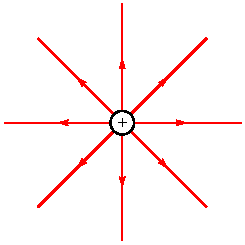
\includegraphics[height=96pt]{pos-charge}
	\end{minipage}
	\begin{minipage}{0.45\linewidth}
		\centering
		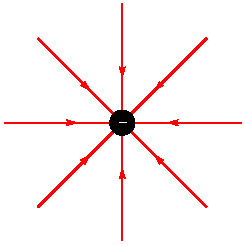
\includegraphics[height=96pt]{neg-charge}
	\end{minipage}
	
	\begin{center}
		radial fields around (a) an isolated positive charge, (b) an isolated negative charge
	\end{center}
\end{figure}

\begin{figure}[htp]
	\vspace*{-18pt}
	\begin{minipage}{0.3\linewidth}
		\centering
		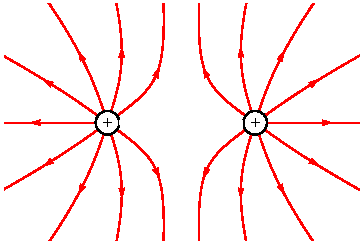
\includegraphics[height=96pt]{like-charges}
	\end{minipage}\hfill
	\begin{minipage}{0.3\linewidth}
		\centering
		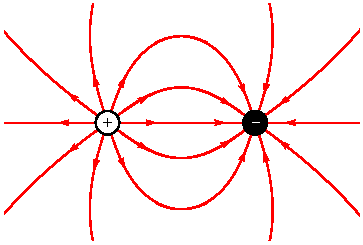
\includegraphics[height=96pt]{opposite-charges}
	\end{minipage}\hfill
	\begin{minipage}{0.3\linewidth}
		\centering
		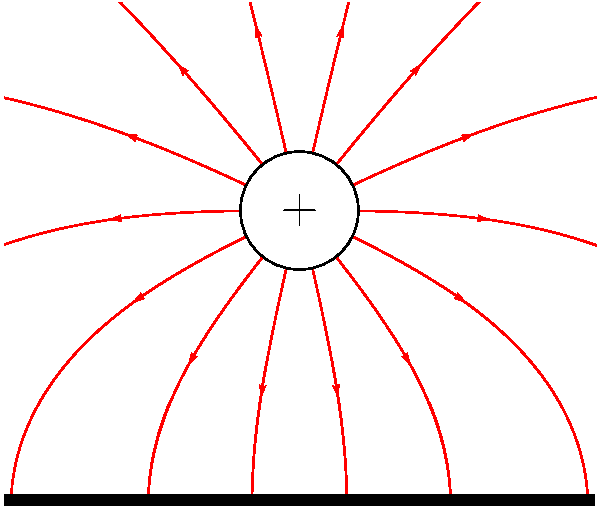
\includegraphics[height=96pt]{sheet-charge}
	\end{minipage}
	
	\begin{center}
		field between (c) two equal and like charges, (d) two equal but opposite charges,
		
		(e) a positive charge and a large conducting sheet that is earthed
	\end{center}
	
	
\end{figure}


\subsection{uniform electric fields}

\begin{marginfigure}
	\vspace{-12pt}
	\begin{center}
		\begin{circuitikz}[european resistors,xscale=0.95]
		\draw[thick] (-1.8,-1) -- (1.8,-1) (-1.8,1) -- (1.8,1);
		\draw[thick] (0,-1) -- (0,-2) node[midway,left]{\Large$-$} -- (3.2,-2)  (3.2,2) -- (0,2) -- (0,1)  node[midway,left]{\Large$+$};
		\draw[thick] (3.2,2) to[battery,l^=$V$] (3.2,-2);
		\foreach \x in {-1.5,-0.5,0.5,1.5} \draw[red,->] (\x,1) -- (\x,-1);
		\draw[<->] (2,-1) -- (2,1) node[midway,right]{$d$};
		\node[purple] at (0,0) {$E$};
		\end{circuitikz}
	\end{center}
	\vspace{-20pt}
\end{marginfigure}

let's take two parallel metal plates and connect them to a high-voltage supply as shown

a charge in the region between the plates experiences a constant force regardless of its location in the field

field strength is constant throughout the region

this field is said to be a \keypoint{uniform electric field}\index{electric field!uniform electric field}

field lines of a uniform field are a set of parallel lines of equal spacing as shown on the right



\cmt if the two plates are separated by a distance of $d$, and a p.d. of $V$ is applied across them

then magnitude of field strength of the uniform field is given by: $\boxed{ E = \frac{V}{d}}$

\noindent\textbf{proof:} work done to bring a test charge $q$ from positive plate to negative plate: $ W=Fd=Eqd $

the change in electric potential energy is: $ \Delta E_p = q V$ (check \S\ref{ch:potential-difference} for meaning of p.d.)

work-energy theorem tells us these two must be equal: $ Eqd = qV$, so we find: $ {E=\frac{V}{d}} $


\cmt electric field between metal plates points from high potential towards low potential

\example{The following examples show the set-up of two uniform electric fields.}

\begin{figure}[ht]
	\centering
	\begin{minipage}{0.45\textwidth}
		\centering
		\begin{tikzpicture}
		\draw[thick] (-1.8,-1) -- (1.8,-1) (-1.8,1) -- (1.8,1);
		\draw[thick,white] (0,-1) -- (0,-1.1) node[ground]{};
		\draw[thick] (0,-1) -- (0,-1.5) node[below]{$-50$ V} (0,1.5) node[above]{$+30$ V} -- (0,1)  ;
		\foreach \x in {-1.5,-0.5,0.5,1.5} \draw[red,->] (\x,1) -- (\x,-1);
		\draw[<->] (2.25,-1) -- (2.25,1) node[midway,right]{10 cm};
		\node[purple] at (0,0) {$E$};
		\end{tikzpicture}
		\begin{equation*}
			E = \frac{V}{d} = \frac{(+30)-(-50)}{0.10} = 800\NpC
		\end{equation*}
	\end{minipage}\hfil
	\begin{minipage}{0.45\textwidth}
		\centering
		\begin{tikzpicture}
		\draw[thick] (-1.8,-1) -- (1.8,-1) (-1.8,1) -- (1.8,1);
		\draw[thick,white] (0,-1) -- (0,-1.5) node[below]{$-50$ V} (0,1.5) node[above]{$+30$ V} -- (0,1)  ;
		\draw[thick] (0,-1) -- (0,-1.1) node[ground]{} (0,1.5) node[above]{$-60$ V} -- (0,1) ;
		\node[right] at (0.3,-1.55) {earthed ($V_0=0$)};
		\foreach \x in {-1.5,-0.5,0.5,1.5} \draw[red,<-] (\x,1) -- (\x,-1);
		\draw[<->] (2.25,-1) -- (2.25,1) node[midway,right]{12 cm};
		\node[purple] at (0,0) {$E$};
		\end{tikzpicture}
		\begin{equation*}
		E = \frac{V}{d} = \frac{0-(-60)}{0.12} = 500\NpC
		\end{equation*}
	\end{minipage}
\end{figure}


\example{Two horizontal parallel plate conductors are separated by 1.5 cm in air. A potential difference of 36 V is applied across the plates. Compare the electric force and gravitational force acting on a proton between the plates.}

\sol electric field strength: $E = \frac{V}{d} = \frac{36}{1.5\times10^{-2}} = 2400 \NpC$

electric force: $F_E = Eq = 2400 \times 1.60\times10^{-19} \approx 3.84\times10^{-16} \text{ N}$

weight of the proton: $W = mg = 1.67\times10^{-27} \times 9.81 \approx 1.64\times10^{-26} \text{ N}$

this shows electric force on proton are much stronger than gravitational forces

when dealing with motion of sub-atomic particles (e.g., protons, electrons, etc.) in an electric field, effects of gravity can therefore be ignored \eoe



\subsection{equilibrium between electric force and weight}


\begin{marginfigure}
	\vspace{-16pt}
	\begin{center}
		\begin{tikzpicture}[xscale=1.1,yscale=1.35]
		\draw[thick] (-2,-1) -- (2,-1) (-2,1) -- (2,1);
		\draw[thick] (0,-1.6) -- (0,-1) node[midway,right]{\Large$+$} (0,1) -- (0,1.6) node[midway,right]{\Large$-$};
		\foreach \x in {-1.8,-0.6,0.6,1.8} \draw[red,->] (\x,-1) -- (\x,1);
		\draw[blue,thick,->] (0,0) -- (0,-0.75) node[right]{$W$};
		\draw[blue,thick,->] (0,0) -- (0,0.75) node[right]{$F_E$};
		\shade [ball color = green] (0,0) circle (0.08) node[left]{$+q$};
		\node[red] at (2.1,0.6) {$E$};
		\end{tikzpicture}
	\end{center}
	\vspace{-20pt}
\end{marginfigure}

a charged particle (e.g., a dust particle or an oil droplet) can be held stationary in a uniform electric field

electric force is in equilibrium with weight of particle

{
	\centering
	
	$ F_E = W \RA Eq = mg $
	
}

\noindent where field strength $E$ is given by: $E = \frac{V}{d}$

note that equilibrium is possible only if $F_E$ acts in opposite direction to $W$, so direction of the applied field depends on polarity of the charged particle



\newpage


\example{A uniform electric field is set up between the two parallel oppositely-charged metal plates separated by 8.0 cm. An oil droplet of mass 0.040 g and charge $-20$ nC is placed in the field. The droplet stays at rest. (a) Find the strength and the direction of the electric field. (b) What is the voltage required to produce this field? (c) If the separation between the plates is reduced, what would happen to the oil droplet?}

\sol (a) equilibrium so electric force equals weight: $F_E = mg = 0.050 \times 10^{-3} \times 9.81 \approx 3.92 \times 10^{-4} \text{ N}$

\hspace*{1.2em} field strength: $E = \frac{F_E}{q} = \frac{ 3.92 \times 10^{-4} }{ 20 \times 10^{-9}} \approx 1.96 \times 10^{4} \NpC$

\hspace*{1.2em} $F_E$ must act upwards for equilibrium, but droplet is negatively-charged

\hspace*{1.2em} so electric field acts in the downward direction

(b) voltage between the plates: $V = E d = 1.96 \times 10^{4} \times 8.0 \times 10^{-2} \approx 1.57 \times 10^3 \text{ V}$

(c) smaller separation means greater field strength, so greater electric force

\hspace*{1.2em} $F_E > mg$ so resultant force acts upwards, droplet will accelerate upwards \eoe



\subsection{deflection of charged particle in uniform fields}

\begin{marginfigure}
	\vspace{-21pt}
	\begin{center}
		\begin{tikzpicture}[scale=1]
		\draw[very thick] (-2,-1) -- (2,-1) (-2,1) -- (2,1);
		\foreach \x in {-1.8,-0.6,0.6,1.8} \draw[red,->] (\x,-1) -- (\x,1);
		\draw[thick,blue,->] (0,-0.35) -- (0,0.7) node[below right]{$F$};
		\shade [ball color = green,dashed] (0,-0.35) circle (0.08);
		\draw [thick,blue!50,domain=-2:2,samples=20,smooth,variable=\x] plot (\x,{0.12*(\x-1)*(\x-1)-0.5});
		\node[red] at (2.1,0.6) {$E$};
		\draw[<->] (-3,0.4) node[left]{$y$} -- (-3,-0.4) -- (-2.2,-0.4) node[below]{$x$};
		\end{tikzpicture}
	\end{center}
	\vspace{-15pt}
\end{marginfigure}

charged particle travelling in a uniform electric field would in general undergo a \emph{projectile-like} motion

we set up the coordinates such that electric field is along the $y$-axis, and $x$-axis is in the normal direction

we denote $x_0$, $y_0$ and $u_x$, $u_y$ as initial displacements and initial velocities at $t=0$

electric force only acts in $y$-direction, no force acts in $x$-direction

\begin{compactenum}
	\item[--] in $x$-direction, particle maintains a constant velocity: $v_x = u_x$, $\,\, x = x_0 + u_x t$
	
	\item[--] in $y$-direction, particle accelerates uniformly: $v_y = u_y + a t$, $\,\, y=y_0 + u_y t + \frac{1}{2}at^2$
	
	where acceleration in $y$-direction is given by $ a=\frac{F}{m} = \frac{Eq}{m} \,\,$ (assuming weight is negligible)
\end{compactenum}

so motion of a charged particle in a uniform electric field is analogous with projectile motion in a uniform gravitational field (see \S\ref{ch:projectile}), i.e., trajectory of charged particle is \emph{parabolic}


\begin{marginfigure}
	\vspace{-15pt}
	\begin{center}
		\begin{tikzpicture}[scale=.96]
		\draw[very thick] (-2,-1) -- (2,-1) (-2,1) -- (2,1);
		\draw[<->] (-2,-1.8) -- (2,-1.8) node[midway,above] {$L=0.15 \text{ m}$};
		\draw[<->] (2.8,-1) -- (2.8,1) node[midway,right] {$d=0.10 \text{ m}$};
		\foreach \x in {-1.8,-0.6,0.6,1.8} \draw[red,<-] (\x,-1) -- (\x,1);
		\shade [ball color = green] (-3,0) circle (0.08) node[below]{$+q$};
		\draw[thick,blue,->] (0,-0.24) -- (0,-0.9) node[above right]{$F$};
		\shade [ball color = green,dashed] (0,-0.24) circle (0.08);
		\draw[->,thick,purple] (-3.5,0.3) -- (-2.5,0.3) node[midway,above]{$u$};
		\draw [thick,blue!50,domain=-2:2,samples=20,smooth,variable=\x] plot (\x,{-0.04*(\x+2.5)*(\x+2.5)+0.01}) (-2.0,0) -- (-3,0) (2.0,-0.8) -- ++(1,-0.36);
		\node[red] at (-2.1,-0.6) {$E$};
		\end{tikzpicture}
	\end{center}
	\vspace{-18pt}
\end{marginfigure}

\example{A proton enters a uniform field of strength $1.0\times10^4\NpC$ at an initial velocity of $5.0\times10^5\mps$. The initial direction of motion is at right angles to the field. The dimensions of the field are shown in the diagram. (a) What is the time taken for the proton to pass through the field? (b) What is the deviation in the direction of the field during this time? (c) If an electron enters the field with the same initial velocity, describe how the deflection of the electron compares with that of the proton.}

\sol constant horizontal velocity, so time taken: $t = \frac{L}{u} = \frac{0.15}{5.0\times10^5} = 3.0\times10^{-7} \text{ s}$

\eqyskip constant acceleration in direction of field: $
a = \frac{F}{m} = \frac{Eq}{m} = \frac{1.0\times10^4\times1.6\times10^{-19}}{1.67\times10^{-27}} \approx 9.58\times10^{11}\mpss $

\eqyskip displacement moved in this direction: $
\Delta y=\frac{1}{2}at^2 = \frac{1}{2} \times 9.58\times10^{11} \times (3.0\times10^{-7})^2 \approx 0.043 \text{ m} $

electron would experience a much greater deflection in the opposite direction

\begin{compactenum}
	\item[--] electron has opposite charge to proton, so deflect in the opposite direction
	
	\item[--] mass of electron is much smaller, so much greater acceleration
	
	time spent in the field is the same, so electron has much greater deflection \eoe
\end{compactenum}




\subsection{polar molecules in uniform electric fields}

centre of positive and negative charges for a molecule do not necessarily overlap

this molecule is still electrically neutral, i.e., it has a zero net charge

such a molecule is called a \emph{polar molecule}, and it could be affected by an electric field 


\begin{marginfigure}
	\vspace{-24pt}
	\begin{center}
		\begin{tikzpicture}[scale=1.8]
		\draw[thick] (-1.25,-1) -- (1.25,-1) (-1.25,1) -- (1.35,1);
		\draw[thick] (0,-1.5) -- (0,-1) node[midway,right]{\Large$-$} (0,1) -- (0,1.5) node[midway,right]{\Large$+$};
		\foreach \x in {-.9,.9} \draw[red,->] (\x,-1) -- (\x,1);
		\node[red] at (1.1,0.6) {$E$};
		\draw[brown,thick,rotate=35] (0,0) ellipse (0.6 and 0.3);
		\node[brown] at (38:0.35) {$-$};
		\node[brown] at (218:0.35) {$+$};
		\draw[thick, blue,->] (38:0.35) ++ (0,0.1) --++ (0,0.5) node[below right]{$F$};
		\draw[thick, blue,->] (218:0.35) ++ (0,-0.1) --++ (0,-0.5) node[above left]{$F$};
		\draw [dashed] (38:0.35) ++ (0,-0.1) --++ (0,-0.9);
		\draw [Green, <->] (38:0.35) ++ (-0.024,-0.9) --++ (-0.5,0) node[midway, above]{$L_\perp$};
		\end{tikzpicture}
	\end{center}
	\vspace{-20pt}
\end{marginfigure}

the diagram shows a polar molecule in a uniform field

force on centre of positive charge and force on centre of negative charge are labelled as shown

this is a pair of equal but opposite forces

so they give rise to a resultant \emph{torque/moment}

recall \emph{torque of couple} is defined as one force times perpendicular distance between the force pair (see \S\ref{ch:torque-of-couple})

{
	\centering
	
	$\tau = F_E L_\perp \RA \tau Eq L_\perp$
	
}

this torque would cause the polar molecule to \emph{rotate}


\chapter{Sub-atomic Particles}

\section{atomic structure}

\subsection{atomic model}\label{ch:atomic-model}

\begin{marginfigure}{r}
	\vspace*{5pt}
	\centering
	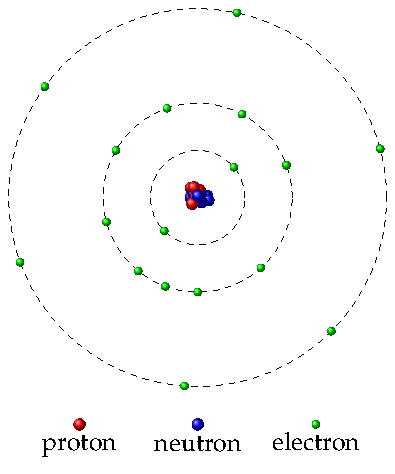
\includegraphics[height=180pt]{atomic-model.pdf}
	\vspace*{-20pt}
\end{marginfigure}

all matter is composed of tiny particles called \keypoint{atoms}

each different element has its own type of atom

the diagram below illustrates a simple atomic model\index{atomic model}


\cmt at centre of each atom is the \keypoint{nucleus}\index{nucleus}

\cmt radius of an atom $\sim 10^{-10} \sim 10^{-9} \text{ m}$

radius of a nucleus $\sim 10^{-15} \sim 10^{-14} \text{ m}$

\cmt particles that make up a nucleus are called \keypoint{nucleons}\index{nucleon}

nucleons come in two types, \keypoint{protons} and \keypoint{neutrons}\index{proton}\index{neutron}

\cmt outside the nucleus are the \keypoint{electrons}\index{electron}

electrons move around the nucleus in a \emph{cloud}

\cmt protons, neutrons and electrons are the building blocks of all atoms and hence the building blocks for all matter

\cmt properties of protons, neutrons and electrons are listed below

\begin{compactenum}
	\item[--] charge of each proton and electron is the elementary charge unit: $e = 1.60 \times10^{-19} \text{ C}$
	
	\item[--] neutron has zero charge
	
	\item[--] a proton has very similar mass as a neutron
	
	\item[--] electron has much smaller mass than a nucleon (proton or neutron)
\end{compactenum}

\begin{center}
	\begin{tabular}{|C{3.5cm}|C{1.6cm}|C{3.5cm}|C{2.8cm}|}
		\hline subatomic particle & charge & mass & location found \\ 
		\hline proton & $+e$ & $m_p = 1.67 \times 10^{-27}$ kg & nucleus \\ 
		\hline neutron & 0 & $m_n = 1.67 \times 10^{-27}$ kg & nucleus \\ 
		\hline electron & $-e$ & $m_e = 9.11 \times 10^{-31}$ kg & in outer atom \\ 
		\hline 
	\end{tabular}
\end{center}

\subsection{$\alpha$-particle scattering experiment}

experiments were designed to verify if the model gives the right description of an atom

one of the most important experiments carried out was the \keypoint{$\alpha$-particle scattering experiment}\index{$\alpha$-particle scattering experiment}

under the direction of \emph{Ernest Rutherford}, \emph{Hans Geiger} and \emph{Ernest Marsden} studied atomic structure by firing $\alpha$-particle beam towards a thin gold foil  at the University of Manchester

\begin{figure}[!ht]
	\centering
	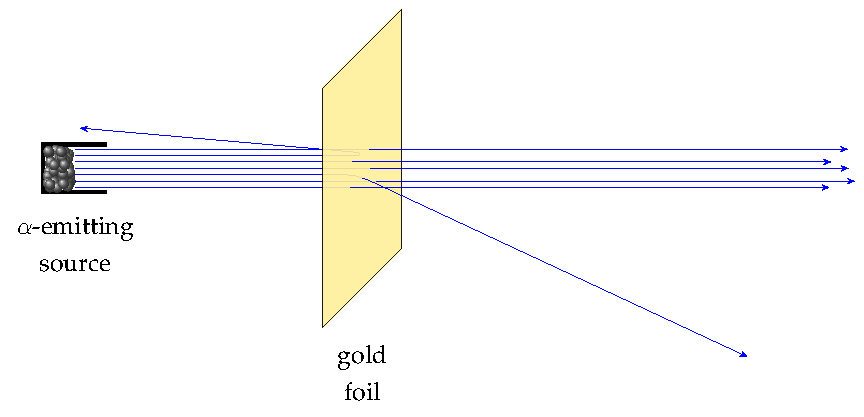
\includegraphics[height=180pt]{alpha-scattering}
	\caption*{Rutherford's $\alpha$-particle scattering experiment}
\end{figure}

\begin{figure}[!ht]
	\centering
	\begin{tikzpicture}[scale=1.33]
		\shade[ball color=Gold] (0,0) circle (.2);
		\node[right, twoline] at (0.3,0) {gold\\nucleus}; 
		\draw[blue,->] (-4,0.03) -- (-0.4, 0.03) arc(-90:86:0.04) --++ (176:2.5);
		\draw[blue,->] (-4,1) -- (3, 1);
		\draw[blue,->] (-4,-1.2) -- (3, -1.2);
		\draw[blue,->] (-4,-0.5) -- (-1,-0.5) arc(90:65:4) --++ (-25:2.4);
	\end{tikzpicture}
	
	\caption*{paths of $\alpha$-particles as they approach and pass by a gold nucleus}
\end{figure}




\cmt the main experimental results of the experiments are

\begin{compactitem}
	\item[--] most $\alpha$-particles pass straight through the foil with almost no deflection
	
	\item[--] very few $\alpha$-particles (about 1 in $10^4$) are deflected by large angles.
\end{compactitem}

\cmt to explain the observations, Rutherford concluded the following about nature of atoms

\begin{compactitem}
	\item[--] most space in an atom is empty
	
	(so most $\alpha$-particles merely pass through empty space without deflection)
	
	\item[--] there is a tiny positively-charged core, called the nucleus, at centre of an atom
	
	(so only a small fraction of $\alpha$-particles would interact with the nucleus)
	
	\item[--] almost all mass of the atom is concentrated in the nucleus
	
	(so interaction is influential if nucleus happens to sit on the path of $\alpha$-particle beam)
\end{compactitem}

based on these understandings, Rutherford proposed the atomic model introduced in \S\ref{ch:atomic-model}

this model is now known as \emph{Rutherford's model}, or \emph{planetary model of the atom}

	Before Ernest Rutherford, the most popular atomic model at the time was proposed by \emph{J. J. Thompson} of the Cavendish Lab at the University of Cambridge. Thompson first discovered electrons from cathode rays. He showed that electrons are negatively-charged and hence proved that an atom is made up of electrons and something that carries positive charges. He suggested that electrons are evenly distributed in a positive cloud of matter, which is now called the \emph{plum-pudding model}.
	
	To verify this model, Rutherford's group set out and designed the gold foil experiment. The plum-pudding model predicts that deflection of $\alpha$-particles should be uniformly distributed around the central beam, but there is no reason that an $\alpha$-particle would undergo a large change in its direction of motion, like a cannonball hitting a piece of paper and rebounding backwards. The results of the scattering experiment meant that the plum-pudding model had to be overturned. In order to explain the experimental observations, Rutherford then put forward the new model which now bears his name.
\footnote{
	 Rutherford originally suggested that electrons rotate around the nucleus in \emph{circular} orbits due to attractive electrostatic force, like the planets orbit around the sun. This is why Rutherford's model of atomic structure is also called \emph{the planetary model of the atom}.
	 
	 However, later studies showed that Rutherford's model had its own problems. Classical electromagnetic theory suggests that any charged particle in accelerated motion would radiate energy, so the orbiting electrons will gradually lose all its energy and fall into the nucleus. An atom can never be stable if the Rutherford's model is correct. The full description of the atomic structure requires the understanding of the \emph{quantum} behaviour of electrons, which are described by \emph{probability waves}. Electrons actually do not move in circular orbits but have a certain probability to be anywhere in space at any time, forming an \emph{electron cloud}.
 }




\subsection{nuclide notation}

\keypoint{nuclides} are specific types of atoms or nuclei

a nuclide is uniquely defined by its \keypoint{proton number} $Z$ and its \keypoint{nucleon number} $A$

a nuclide is usually denoted as $\boxed{_Z^A X}$, where $X$ is the chemical symbol for the element

\cmt by definition, $Z$ gives number of protons, $A$ gives number of nucleons

as a consequence, number of neutrons is given by $N = A-Z$

\cmt proton number $Z$ can be further interpreted as \keypoint{charge number} of the particle \index{charge number}

recall each proton carries charge $+e$, and neutrons are chargeless

so $Z$ further determines electrical charge of the nucleus: $\boxed{Q = +Ze}$

this extension will be important when we deal with other particles later in this chapter

\cmt nucleon number $A$ can be interpreted as \keypoint{mass number} of the particle \index{mass number}

each proton and neutron is of approximately the same mass

so mass of nucleus is determined by total number of protons and neutrons: $\boxed{m = A\text{u}}$

where $1 \text{ u} = 1.66\times10^{-27} \text{ kg}$ is the \keypoint{unified atomic mass unit}
\footnote{Note that the unified atomic mass ($1.661\times10^{-27} \text{ kg}$), formally defined as one twelfth of the mass of an carbon-12 atom, is slightly less than the mass of a \emph{free} proton ($m_p=1.673\times10^{-27} \text{ kg}$ or that of a \emph{free} neutron ($m_n=1.675\times10^{-27} \text{ kg}$). This is because energy goes out when protons and neutrons combine to form a nucleus, and this would be associated with a decrease in the mass as suggested by \emph{Albert Einstein's mass-energy equivalence principle}. You can think of $\text{u}$ as the average mass of a proton or a neutron when a group of them squeeze together. If you want to find out the mass of a nucleus, you should use $\text{u}$. But if you are dealing with a single proton or a single neutron, you should use $m_p$ and $m_n$ instead.}

\cmt using this notation, protons, neutrons and electrons can be represented by: $ \boxed{^1_1\text{p}}$, $\boxed{^1_0\text{n}}$, $\boxed{^{\phantom{-}0}_{-1}\text{e}} $

\example{The nuclide uranium-238 can be denoted by $^{238}_{\phantom{2}92}\text{U}$. (a) State its proton number and its neutron number. (b) Find the charge and mass of the uranium-238 nucleus.}

\begin{soln} proton number: $Z=92$

neutron number: $N=A-Z=238-92=146$

nuclear charge: $Q=+Ze=+92\times1.60\times10^{-19}\approx1.47\times10^{-17}\text{ C}$

mass of nucleus: $m=A\text{u} = 238 \times 1.66\times10^{-27} \approx 3.95 \times 10^{-25}\text{ kg}$ \eoe


\example{Radius of a copper-64 nucleus is $4.8\times10^{-15} \text{ m}$. Calculate the mean nuclear density.}

\solc\begin{equation*}
	\rho = \frac{m}{V} = \frac{A\text{u}}{\frac{4}{3}\pi r^3} = \frac{64 \times 1.66\times10^{-27}}{\frac{4}{3}\pi \times (4.8x10^{-15})^3} \RA \rho \approx 2.3 \times 10^{17} \text{ kg m}^{-3}
\end{equation*}

this is much greater than density of a copper block (about $8.9 \times  10^3 \text{ kg m}^{-3}$)

we can therefore infer that the nucleus indeed takes most mass of the atom \end{soln}


\subsection{chemical properties of elements}

chemical properties of an atom depend on the number of electrons

\cmt proton number $Z$ also gives the \keypoint{atomic number} of the element

in a neutral atom, there are same number of protons as electrons

so atoms of same chemical properties, i.e., atoms of same element have same proton number

\cmt atoms of same chemical properties can have different nuclei

\keypoint{isotopes} of same element have same number of protons but different number of neutrons\index{isotope}





\example{State and explain whether carbon-12 ($^{12}_{\phantom{1}6}\text{C}$) and carbon-14  ($^{14}_{\phantom{1}6}\text{C}$) are different isotopes of the same element.}

\begin{soln} both carbon-12 and carbon-14 atoms have 6 protons

but carbon-12 has 6 neutrons, carbon-14 has 8 neutrons

same proton number but different neutron number, so different isotopes of same element \end{soln}




\subsection{radioactivity}

\subsection{radioactive decays}

if a nucleus is unstable then it may break down by releasing radiation from the nucleus

this process is called \keypoint{radioactive decay}\index{radioactive decay}

\cmt three most common types of radioactive decays are $\alpha$-decay, $\beta$-decay and $\gamma$-decay

\cmt radioactive decays are \emph{spontaneous}

decay events are independent of outside conditions, such as temperature, pressure, etc.

whether one nucleus is about to decay is also independent of the other nuclei around it

radioactive decays only depend on the internal stability of the nucleus

\cmt radioactive decays are \emph{random}

one cannot predict when and which nucleus will decay

an unstable nucleus might decay at any time

whether or not decay occurs can only be given by probabilities





\subsection{properties of $\alpha$-, $\beta$- \& $\gamma$-radiation}

\subsection*{nature of \texorpdfstring{$\alpha$}{\textalpha}-radiation}

$\alpha$-particles are \emph{helium nuclei}, each made up of two protons and two neutrons\index{radioactive decay!$\alpha$-decay}

an $\alpha$-particle therefore carries a positive charge of 2$e$, and a mass of 4u

$\alpha$-particles emitted from a given source travel at almost the same speed

speed of $\alpha$-particles is usually less than one-tenth of the speed of light

\subsection*{nature of \texorpdfstring{$\beta$}{\textbeta}-radiation}


$\beta$-radiation is a beam of high-speed \emph{electrons}\index{radioactive decay!$\beta$-decay}

$\beta$-particle is negatively charged and very light compared with a nucleus

$\beta$-particles travel at very high speeds close to the speed of light

\subsection*{nature of \texorpdfstring{$\gamma$}{\textgamma}-radiation}

$\gamma$-radiation, or $\gamma$-photon, is a high-frequency electromagnetic wave\index{radioactive decay!$\gamma$-decay}

$\gamma$-radiation is electrically neutral and has no mass

like any other electromagnetic wave, $\gamma$-radiation travels at the speed of light in vacuum

\subsection*{brief summary for nature of \texorpdfstring{$\alpha$}{\textalpha}-, \texorpdfstring{$\beta$}{\textbeta}- \& \texorpdfstring{$\gamma$}{\textgamma}-radiation}



\begin{center}
	{\renewcommand{\arraystretch}{1.2}
	\begin{tabular}{|C{2cm}|C{2.8cm}|C{2.8cm}|C{4.2cm}|}
	\hline  & $\alpha$-radiation & $\beta$-radiation & $\gamma$-radiation \\ 
	\hline nature & helium nucleus & electron & electromagnetic wave \\ 
	\hline notation & $^4_2\alpha$ & $^{\phantom{-}0}_{-1}\beta$ & $^0_0\gamma$ \\
	\hline mass & 4u & $\frac{1}{1800}\text{u} \approx 0$ & 0 \\[4pt]
	\hline charge & $+2e$ & $-e$ & 0 \\ 
	\hline speed & $0.1c$ & $0.99c$ & $c$ \\
	\hline
    \end{tabular}
    }
\end{center}

%\begin{question}
%	Some radioactive sources are found to contain helium gas. How do you explain that?
%\end{question}

%\begin{question}
%	$\alpha$-particles are used in the scattering experiment to investigate the structure of an atom. Is it appropriate to use a $\beta$-emitting source to do the same experiment? Explain your reasons.
%\end{question}


\example{If a single beam of $\alpha$-particles, $\beta$-particles and $\gamma$-radiation is sent into a uniform electric field as shown, sketch and explain the paths of the beam.}

\begin{figure}[ht]
	\centering
	\begin{tikzpicture}
	\draw[thick] (-3,-1) -- (3,-1) (-3,1) -- (3,1);
	\draw[thick] (0,-1) -- (0,-2) node[midway, right] {$-$};
	\draw[thick] (0,1) -- (0,2) node[midway, right] {$+$};
	\draw[thick, purple, ->] (-4,0) -- (4, 0) node[right] {$\gamma$};
	\draw[thick, Green, ->] (-4,0.05) -- (-3,0.05) parabola (-2.4,1) node[below right]{$\beta$};
	\draw[thick, blue, ->] (-4,-0.05) -- (-3,-0.05) parabola (3,-0.85) --++ (-14.93:1) node[right] {$\alpha$};
	\end{tikzpicture}
\end{figure}

\begin{soln} $\gamma$-radiation has zero charge, so it is not affected by electric field

$\alpha$-radiation is positively-charged, so it deflects towards the negative plate

$\beta$-radiation is negatively-charged, so it deflects towards the positive plate

$\beta$-particles are much lighter, so they have greater deflection \end{soln}


\subsection*{penetration \& ionising power}

different radiation have different abilities to pass through materials

$\alpha$-, $\beta$- and $\gamma$- radiation are able to knock out orbital electrons from an atom

so radiation can cause the originally neutral atom to become charged

this process is called \keypoint{ionising}\index{ionising power}

\cmt greater ionising ability would imply lower penetration power

radiation loses energy as it passes through a substance

this energy loss is transferred to electrons, causing ionisation of atoms

so the faster radiation gives up its energy, the lower the penetration ability

\cmt $\gamma$-radiation is very penetrative but has very weak ionising power 

$\gamma$-radiation is not charged, and hence it does not interact strongly with electrons

a $\gamma$-photon loses all its energy in single collision and gets absorbed

i.e., one $\gamma$-photon can only ionise one atom

so it has few collisions with electrons, so $\gamma$-radiation is not very ionising

\cmt $\alpha$- and $\beta$-radiation more ionising than $\gamma$-radiation

this is because $\alpha$- and $\beta$-radiation are charged, making them interact with electrons more easily

\cmt $\alpha$-particles are highly ionising

recall $\alpha$-particles are much more massive than electrons

so one $\alpha$-particle can knock out many electrons before it loses all of its kinetic energy

also $\alpha$-particles travel at low speeds, so frequent collision events take place in short range

therefore $\alpha$-radiation has strong ionising ability but weak penetration power

\cmt the table below summarises penetration and ionising power of radioactive radiation

\begin{center}
	\begin{tabular}{|C{3cm}|C{3.2cm}|C{3.2cm}|C{3.2cm}|}
		\hline  & $\alpha$-radiation & $\beta$-radiation & $\gamma$-radiation \\ 
		\hline \multirow{2}{3.2cm}[-20pt]{penetration power} & low & fair & high \\
		 & stopped by thick cardboard or a few centimetres of air & stopped by metal plates of a few millimetres thick & stopped by thick lead or concrete of a few centimetres\\
		\hline ionising power & high & fair & low \\ 
		\hline
	\end{tabular} 
\end{center}



\subsection{laws of conservation}

some of the conserved quantities during any decay process are:

\cmt conservation of \emph{electric charge}

\cmt conservation of \emph{charge number} ($Z$)\index{charge number}

this is a consequence of the conservation of electric charge

\cmt conservation of \emph{mass-energy}\index{mass-energy conservation}

Einstein's theory of relativity suggests that mass is equivalent to energy $E=mc^2$

for any naturally occurring nuclear decay process that releases energy, total mass of product particles will be \emph{less} than that of the original particles

reduction in mass becomes of the energy released, which can be kinetic energy of product particles, electromagnetic energy of $\gamma$-radiation emitted, etc.

\cmt conservation of \emph{mass number} ($A$)\index{mass number}

notice that mass number is not exactly proportional to mass of nucleus

mass itself is not conserved during the reaction but only the mass number is conserved

\cmt conservation of \emph{momentum} (review \S\ref{ch:momentum-conservation} if needed)

no external force is involved in nuclear decays, so total momentum is also constant

more specifically, when a stationary nucleus decays into two product particles, for example, the two product particles after an $\alpha$-decay process should move off with equal but opposite momenta


\subsection{decay equations}

using nuclide notation, radioactive decay processes can be described by \emph{decay equations}

the conserved quantities provide a simple guideline to write the decay equations 

\begin{compactenum}
	\item[--] sum of charge numbers ($Z$) on both sides of the equation should add up
	
	\item[--] sum of mass numbers ($A$) on both sides of the equation should add up
\end{compactenum}


The first reported nuclear reaction was credited to Ernest Rutherford. By firing $\alpha$-particles into pure nitrogen, Rutherford observed the ejection of hydrogen nuclei from the gas, which is now regarded as the discovery of protons. This reaction can be given by:
\begin{equation*}
_{\phantom{0}7}^{14} \text{N} + _2^4 \alpha \longrightarrow _{\phantom{0}8}^{17} \text{O} + _{1}^{1} \text{p} 
\end{equation*} 


One reaction that is widely used to power nuclear reactors is the induced fission of uranium-235. The reaction can be triggered by bombarding the uranium-235 nuclei with slow neutrons. The uranium nucleus would split up into two lighter nuclei and release a large amount of energy. One of such reactions can be described by:
\begin{equation*}
 _{\phantom{0}92}^{235} \text{U} + _0^1 \text{n} \longrightarrow _{\phantom{0}56}^{141} \text{Ba} + _{36}^{92} \text{Kr} + 3_0^1 \text{n} 
\end{equation*} 




\subsection*{equation for \texorpdfstring{$\alpha$}{\textalpha}-decays}\index{radioactive decay!$\alpha$-decay}

if a nuclide $_Z^A X$ undergoes $\alpha$-decays, then we have:
\begin{equation*}
\boxed{_Z^A X \longrightarrow _{Z-2}^{A-4} Y + _2^4\alpha}
\end{equation*}

the original nucleus lost two protons and two neutrons during the decay

on both sides of the equation, there are $Z$ protons and $(A-Z)$ neutrons

therefore $\alpha$-decay simply is an $\alpha$-particle escaping from the nucleus



\example{The process in which a uranium-238 nucleus naturally decays into a thorium-234 nucleus through $\alpha$-emission can be written as:}
\begin{equation*}
	_{\phantom{0}92}^{238} \text{U} \longrightarrow _{\phantom{0}90}^{234} \text{Th} + _2^4\alpha 
\end{equation*}



\subsection*{equation for \texorpdfstring{$\gamma$}{\textgamma}-decays}\index{radioactive decay!$\gamma$-decay}

$\gamma$-radiation has zero charge and zero mass, so decay equation is very straightforward:
\begin{equation*}
\boxed{_Z^A X \longrightarrow _{Z}^{A} X + _0^0\gamma}
\end{equation*}

since $\gamma$-radiation is pure energy, so there is no change of structure of the nucleus in any way



\subsection*{problems with \texorpdfstring{$\beta$}{\textbeta}-decays}\index{radioactive decay!$\beta$-decay}

for $\beta$-decays, one might attempt to write: $
	_Z^A X \longrightarrow _{Z+1}^{\phantom{1+}A} Y + _{-1}^{\phantom{+}0}\beta$ 

on the left, nuclide $X$ has $Z$ protons and $(A-Z)$ neutrons

but on the right, nuclide $Y$ has $(Z+1)$ protons and $(A-Z-1)$ neutrons

one neutron has transformed into a proton through giving off an electron: $_0^1 \text{n} \longrightarrow _1^1 \text{p} + _{-1}^{\phantom{+}0}\text{e} \,\, \text{???}$

but how can neutrons and protons transform into one another?!

further experiments show that $\beta$-particles emitted for same source have \emph{a range of speeds}

this seems to indicate that energy released from a $\beta$-decay can be indefinite

both considerations imply something is wrong, our understanding of $\beta$-decay is not complete

\begin{compactenum}
	\item[--] protons and neutrons cannot be the most fundamental particles of nature
	
	there must exist some more fundamental constituent particles
	
	these are now known as \emph{quarks}, we will discuss them in the next section
	
	\item[--] there must be some other unseen particles released during $\beta$-decays
	
	these particles carry off a fraction of the energy released from the reaction
	
	for conservation laws to hold, they must be chargeless and very light (maybe massless)
	
	these ghostly particles are called \keypoint{neutrinos}, or more precisely, \keypoint{anti-neutrinos}\index{neutrino}
\end{compactenum}

\cmt we thereby can rewrite the $\beta$-decay equation for nuclide $_Z^A X$:
\begin{equation*}
\boxed{_Z^A X \longrightarrow _{Z+1}^{\phantom{1+}A} Y + _{-1}^{\phantom{+}0}\beta + _0^0 \bar{\nu}} \quad \text{or} \quad \boxed{_0^1 \text{n} \longrightarrow _1^1 \text{p} + _{-1}^{\phantom{+}0}\beta + _0^0 \bar{\nu}} \label{eqn:beta-decay}
\end{equation*}

\cmt distribution of kinetic energy of $\beta$-particles can be then explained

only total energy of $\beta$-particle and anti-neutrino is constant

anti-neutrinos also carry some energy, so $\beta$-particles have a range of energies

\example{Radon $^{222}_{\phantom{2}86}\text{Rn}$ decays in a sequence of processes to form bismuth $^{214}_{\phantom{2}83}\text{Bi}$ by emitting $\alpha$-particles and $\beta$-particles. For the decay chain of each radon nucleus, how many $\alpha$-particles and $\beta$-particles are emitted?}

\begin{soln} let $x$ be number of $\alpha$-particles emitted and $y$ be number of $\beta$-particles emitted
\begin{equation*}
	^{222}_{\phantom{2}86}\text{Rn} \longrightarrow ^{214}_{\phantom{2}83}\text{Bi} + x \cdot ^4_2 \alpha + y \cdot _{-1}^{\phantom{+}0}\beta + y \cdot _0^0 \bar{\nu}
\end{equation*}

\eqyskip mass number and charge number are conserved: $\Bigg\{$

\vspace*{-1.58\baselineskip}\hspace*{218pt} $\begin{array}{l}
4x + 214 = 222\\[-5pt]
2x - y + 83 = 86
\end{array} \RA x = 2$, $y=1$ \end{soln}



\subsection{fundamental particles}

In early 20th century, lots of new subatomic particles were discovered in \emph{cosmic rays} and \emph{particle accelerators}. Many of these particles did not fit into the model where proton, neutrons and electrons are the fundamental building blocks for the physical world. To incorporate these subatomic particles discovered at the time, physicist worked out the \keypoint{Standard Model of particle physics}.\footnote{The theory of the Standard Model was developed in stages since the 1950s, through the work of many great scientists, with the current formulation being finalized in the 1970s.\index{Standard Model}
	\begin{compactitem}
		\item[--] \emph{Chen Ning Yang} and \emph{Robert Mills} developed the concept of \emph{gauge theory}, to provide an explanation for the interaction between elementary particles.
		
		\item[--] \emph{Sheldon Glashow} proposed the symmetry group that forms the basis of the accepted \emph{electroweak theory}, in which the electromagnetic interaction and weak interactions are unified into a single force.
		
		\item[--] \emph{Peter Higgs} and two other groups proposed the \emph{Higgs mechanism} that give rise to mass generation for elementary particles without violating gauge theory through a process called \emph{symmetry breaking}.
		
		\item[--] \emph{Steven Weinberg} and \emph{Abdus Salam} incorporated the Higgs mechanism into Glashow's theory, finalizing the unified electroweak theory.
		
		\item[--] \emph{David Gross}, \emph{Frank Wilczek}, \emph{David Politze}, and many others developed \emph{quantum chromodynamics}, the theory of the strong interaction, into its modern form.
		
		\item[--] $\cdots$
	\end{compactitem}

Being the most accurate accurate scientific theory known to human beings, the Standard Model is now regarded as one of the greatest triumphs of modern physics. The theory not only describes the particles known to scientists, but also predicted new particles, including the \emph{Higgs boson}. }


\subsection{particles \& anti-particles}

for any particle $\text{p}$, there exists an associated \keypoint{anti-particle} $\bar{\text{p}}$\index{anti-particle}

\cmt an anti-particle has the same mass but opposite charge to its counterpart

\cmt when a particle meets its anti-particle, they \keypoint{annihilate} each other and produce two $\gamma$-photons

combined mass-energy of the pair is converted into electromagnetic energy
\footnote{The energy release from the annihilation of  particle pairs could be potentially used a energy source. The idea of using antimatter to power spaceships or weapons can be found in many science fiction stories.}



\example{Suggest the properties of the anti-particle of the electron.}

\begin{soln} anti-particle of electron has same electron mass: $m_e = 9.11\times10^{-31} \text{ kg}$

but it has a positive charge: $q = +e = + 1.60\times10^{-19} \text{ C}$

anti-particle of electron is usually called a \keypoint{positron} (positive electron) with the symbol $\text{e}^+$ \end{soln}


\subsection{quarks \& hadrons}

one type of the elementary matter particle is the \keypoint{quark}\index{quark}

\cmt quarks come in six varieties, or six \keypoint{flavours}

they are \keypoint{up} (u), \keypoint{down} (d), \keypoint{strange} (s), \keypoint{chartm} (c), \keypoint{top} (t), \keypoint{bottom} (b)

\cmt each quark carries an electric charge, as given in the table below

\begin{center}
	{\renewcommand{\arraystretch}{1.35}
		\begin{tabular}{|C{3cm}|C{2cm}|C{2cm}|}
			\hline  & u & d \\
			 quarks & c & s \\
			  & t & b \\
			\hline charge & $+\frac{2}{3}e$ & $-\frac{1}{3}e$ \\[3pt]
			\hline
		\end{tabular}
	}
\end{center}

note that all quarks carry a \emph{fraction} of the elementary charge unit\footnote{Each horizontal line in the table is known as a \emph{generations} of quarks. As you can see, there are three generations of quarks.}

\cmt quarks can combine to form composite particles called \keypoint{hadrons} \index{hadron}

there are two ways that several quarks can make up a hadron

\begin{compactenum}
	\item[--] hadrons can be made up of three quarks (qqq), called \keypoint{baryons} \index{baryon}
	
	members of the baryon family include protons and neutrons
	
	a proton consists of two up quarks and one down quark (uud) \index{proton}
	
	a neutron consists of one up quark and two down quarks (udd) \index{neutron}
	
	\item[--] hadrons can also be made up of one quark and one anti-quark (q$\bar{\text{q}}$), called \keypoint{mesons} \index{meson}
	
	you don't need to memorise any example of meson
	
	you are only required to identify if a particle is a meson given the quark composition
\end{compactenum}

\cmt quarks and hadrons are affected by the \keypoint{strong nuclear force}\index{strong nuclear force}

strong nuclear force is a very short-ranged attractive force

\begin{compactenum}
	\item[--] it is responsible for hold quarks close together to from hadrons

	\item[--] it is also responsible for the attraction between hadrons
	
	for example, protons and neutrons are held together in a nucleus by strong force
	\footnote{For a small nucleus, strength of strong nuclear force is way greater than the electric repulsion between positively-charged protons, hence the force bind protons and neutrons together forming a stable nucleus. However, since the strong nuclear force has a very short range, the repulsive electrostatic force between the protons might dominate the attractive nuclear force for an over-sized nucleus. Such large nuclei become unstable and are likely to undergo \emph{radioactive decays}.}
\end{compactenum}


\cmt quarks only exist in hadrons, i.e., there are no single free quarks in nature\footnote{This is known as the \emph{confinement}, a consequence that is closely related to the fact that interaction between quarks are weak at high energies or smaller length scales but strong at low energies or large length scales, a feature of strong nuclear forces known as \emph{asymptotic freedom}.}


\example{By reference to the quark composition, explain the electric charge of protons and neutrons.}

\begin{soln} charge of proton (uud): $q_\text{p} = 2q_\text{u} + q_\text{d} = 2\times\left(+\frac{2}{3}e\right) + \left(-\frac{1}{3}e\right) = +e$

\eqyskip charge of neutron (udd): $q_\text{n} = q_\text{u} + 2q_\text{d} = \left(+\frac{2}{3}e\right) + 2\times\left(-\frac{1}{3}e\right) = 0$ \end{soln}

\example{A meson has an electric charge of $+e$ and is known to contain an up quark. Determine a possible flavour of the other quark.}

\begin{soln} charge of the other quark is: $(+e) - \left(+\frac{2}{3}e\right) = +\frac{1}{3}e$

this could be an anti-down ($\bar{\text{d}}$), an anti-strange ($\bar{\text{s}}$), or an anti-bottom quark ($\bar{\text{b}}$)\end{soln}



\subsection{leptons}

another type of the elementary matter particle is the \keypoint{lepton}\index{lepton}

\cmt leptons are not affected by strong nuclear forces

\cmt members of the lepton family include electrons (e), neutrinos ($\nu$), muons ($\mu$), taons ($\tau$)\footnote{Just like the quarks, leptons also come in three \emph{generations}. Each generation of leptons consists of an electron-like particle and its associated neutrino.}

in A-Level exams, you only need to know electrons (e) and neutrinos ($\nu$)


\cmt for each particle, one can assign a \keypoint{lepton number} $L$

\begin{compactitem}
	\item[--] a lepton has lepton number $L=+1$
	
	\item[--] an anti-lepton has lepton number $L=-1$
	
	 \item[--]any other particle has lepton number $L=0$
\end{compactitem}

classification of sub-atomic particles within the A-Level syllabus is summarised below\footnote[][-2cm]{This is an over-simplified version of the Standard Model. I only included the particles that you need to know for the A-Level exams. There are a lot of missing pieces that are way beyond the scope of our course, so please don't take this mindmap too seriously.}

\begin{figure*}[ht]
	\centering
	\begin{tikzpicture}
%\draw[help lines, gray!30, step=0.5] (0,-5) grid (15,5);
%\foreach \x in {1,2,...,15} \node[below] at (\x,0) {\x};
%\foreach \y in {-5,-4,...,5} \node[left] at (0,\y) {\y};
	% root / fundamental particles
	\draw (2.5,0.4) -- (3.5,0.4) (4.5, -.6) -- (3.5,-0.6) -- (3.5, 2.5) -- (4.5, 2.5);
	\draw[rounded corners, fill=white] (0.1,-0.3) rectangle (2.5,1.1);
	\draw (1.3,0.4) node[twolinecap] {fundamental\\particles};
	% quarks
	\draw[rounded corners, fill=white] (4.3,2.2) rectangle (5.9, 2.8);
	\draw (5.1, 2.5) node {quarks};	
	\draw (5.0, 2.1) -- (4.6, 1.6);
	\draw (5.2, 2.1) -- (5.6, 1.6);
	\node at (4.6, 1.4) {u};
	\node at (5.6, 1.4) {d};
	\node at (4.6, 0.9) {{\scriptsize $+\frac{2}{3}e$}};
	\node at (5.6, 0.9) {{\scriptsize $-\frac{1}{3}e$}};
	% leptons
	\draw[rounded corners, fill=white] (4.3,-.4) rectangle (5.9, -1.0);
	\draw (5.1, -.7) node {leptons};
	\draw (5.0, -1.1) -- (4.6, -1.6) node[below]{e};
	\draw (5.2, -1.1) -- (5.6, -1.6) node[below]{$\nu$};
	\node at (4.6, -2.2) {{\scriptsize $-e$}};
	\node at (5.6, -2.2) {{\scriptsize $0$}};
	% hadrons
	\draw[dashed, ->] (5.9, 2.5) -- (8.1,2.5) node[midway, above]{make up};
	\draw[rounded corners, fill=white] (8.1,2.2) rectangle (9.9, 2.8);
	\draw (9, 2.5) node {hadrons};
	% baryons
	\draw (9.9, 2.5) -- (10.5, 2.5) -- (10.5, 3.5) -- (12, 3.5) node[midway, above]{(qqq)};
	\draw[rounded corners, fill=white] (12,3.2) rectangle (13.8, 3.8);
	\draw (12.9, 3.5) node {baryons};
	\draw (12.8, 3.1) -- (12.4, 2.6) node[below]{p};
	\draw (13.0, 3.1) -- (13.4, 2.6) node[below]{n};
	% mesons
	\draw (10.5, 2.5) -- (10.5, 1.5) -- (12, 1.5) node[midway, above]{(q$\bar{\text{q}}$)};
	\draw[rounded corners, fill=white] (12,1.2) rectangle (13.8, 1.8);
	\draw (12.9, 1.5) node {mesons};
	\end{tikzpicture}
	\caption{a coarse guide for classifying sub-atomic particles in A-Level physics}
\end{figure*}



\subsection{\texorpdfstring{$\beta$}{\textbeta}-decays}\index{radioactive decay!$\beta$-decay}

there exists positron, anti-particle of electron, so there are two types of $\beta$-particles: $\beta^-$ and $\beta^+$

hence two types of $\beta$-decays are possible: $\beta^-$-decay and $\beta^+$-decay



\subsection*{\texorpdfstring{$\beta^-$}{\textbeta\textsubscript{-}}-decay revisited}

a neutron changes into a proton during a $\beta^-$-decay: $\boxed{_0^1 \text{n} \longrightarrow _1^1 \text{p} + _{-1}^{\phantom{+}0}\beta + _0^0 \bar{\nu}} $

we have learned about the quark structures of protons (uud) and neutrons (udd)

therefore $\beta^-$-decay process at a more fundamental level is: $ \boxed{\text{d} \longrightarrow \text{u} + \beta^- + \bar{\nu}} $


\subsection*{\texorpdfstring{$\beta^+$}{\textbeta\textsubscript{+}}-decay}


$\beta^+$-decay occurs when a proton changes into a neutron and emits a positron

$\beta^+$-decay process is described by the equation: $ \boxed{_1^1 \text{p} \longrightarrow _0^1 \text{n} + _{+1}^{\phantom{+}0}\beta + _0^0 \nu} $

in terms of quarks, $\beta^+$-decay can be rewritten as: $ \boxed{\text{u} \longrightarrow \text{d} + \beta^+ + \nu} $

\cmt nature of $\beta$-decay processes is the transformation of quark flavours

the interaction responsible for this transformation is the \keypoint{weak nuclear force}\index{weak nuclear force}

\cmt there is yet another law of conservation -- the \keypoint{conservation of lepton number}

we can use lepton number to predict whether a neutrino or an anti-neutrino is emitted

\example{Verify the conservation of (a) charge number, (b) mass number, and (c) lepton number for the $\beta^+$-decay process: $_1^1 \text{p} \longrightarrow _0^1 \text{n} + _{+1}^{\phantom{+}0}\beta + _0^0 \nu$}

\begin{soln} charge number conservation: $+1 = 0 + (+1) + 0$ \xskip \ding{51}

mass number conservation: $1 = 1 + 0 + 0$ \xskip \ding{51}

lepton number conservation: $0 = 0 + (-1) + (+1)$ \xskip \ding{51}

so this reaction does not violate any of these conservation law \end{soln}


\example{\emph{Electron capture} is a process where an electron in an atom's inner shell is drawn into the nucleus and combines with a proton. The result is to form a neutron and a neutrino. The process can be given by: $_1^1 \text{p} + _{-1}^{\phantom{+}0}\text{e} \longrightarrow _0^1 \text{n} +  + _0^0 \nu$. Show that the process satisfies the conservation of (a) charge number, (b) mass number, and (c) lepton number.}

\begin{soln} charge number conservation: $+1 + (-1) = 0 + 0$  \xskip \ding{51}

mass number conservation: $1 + 0 = 1 + 0$ \xskip \ding{51}

lepton number conservation: $0 + 1 = 0 + 1$  \xskip \ding{51}

so this reaction does not violate any of these conservation law \end{soln}

	
\section{end-of-chapter questions}

\subsection*{atomic structure}

\question{
	List the number of sub-atomic particles in an argon-40 ($^{40}_{18}\text{Ar}$) atom.
}


 



\subsection*{radioactive decays}
	
\question{
	A radioactive source emits a parallel beam of $\alpha$-, $\beta$- and $\gamma$-radiation. A detector sensitive to all forms of radiation has been calibrated for background radiation and is placed just 1 cm from the radioactive source. The detector registers 500 counts s$^{-1}$.  
		
	When the detector is 10 cm from the source, the radiation level drops to 200 counts s$^{-1}$.
	
	When a thin aluminium sheet is placed in front of the detector, the level falls to 50 counts s$^{-1}$.
	
	In what proportion is the source emitting $\alpha$-, $\beta$- and $\gamma$-particles?
}



\subsection*{nuclear equations}

\question{
	An unstable isotope of phosphorus, $_{15}^{30}$P can be produced by bombarding aluminium, $_{13}^{27}$Al, with $\alpha$-particles. What is the by-product of this reaction?
}

\question{
	Carbon-14 ($^{14}_{\phantom{0}6}$ C) undergoes $\beta$-decay and forms an isotope of nitrogen (N). Write down the decay equation using the nuclide notations.
}

\question{
	Radon-222 ($^{222}_{\phantom{2}86}$Rn) undergoes a series of decays and forms lead-210 ($^{210}_{\phantom{2}82}$Pb). 
	How many $\alpha$-particles and $\beta$-particle are emitted during this process?
}

\subsection*{fundamental particles}


\question{
	State the mass and electric charge of an anti-proton.
}

\question{
	$\pi^+$ is a particle with quark structure $u\bar{d}$. (a) State the family of this particle. (b) Show that it carries a charge of $+e$. (c) Suggest the charge of its anti-particle.
}



\question{
	$\Xi^0$ is a particle with quark structure $uss$. (a) State the family of $\Xi^0$. (b) Find its electric charge.
}

\question{
	Magnesium-23 ($^{23}_{12}$Mg) can decay into sodium-23 ($^{23}_{11}$Na). (a) Write down the decay equation using nuclide notation, and specify any other product particles produced. (b) Write an equation for this decay in terms of protons and neutrons. (c) Write an equation for this decay in terms of quark composition. (d) State the name of the force that is responsible for this decay.
}
	



% \chapter{Circular Motion}

\section{Angular quantities}

Movement or rotation of an object along a circular path is called \keypoint{circular motion}, to describe a circular motion, we can use \emph{angular quantities}, which turn out to be more useful than linear displacement , linear velocity , etc.


\subsection{Angular displacement}

\begin{ilight}
	\keypoint{Angular displacement}\index{angular displacement} is angle swiped out by object moving along circular
\end{ilight}

\begin{marginfigure}
	\centering
	\vspace*{-8pt}
	\begin{tikzpicture}[scale=0.8]
		\draw[dotted,thick] (0,0) circle(2);
		\draw[->,thick,blue] (2,0) arc (0:70:2);
		\draw (2,0) -- (0,0) node[midway,below]{$r$} -- (70:2);
		\draw[->,thick] (0.4,0) arc (0:70:0.4);
		\node at (35:0.6) {$\theta$};
		\node at (35:2.2) {$s$};
	\end{tikzpicture}
\end{marginfigure}

unit: $[\theta]=\rad \quad$ (natural unit of measurement for angles)

conversion rule: $2\pi \rad = 360^\circ$

\cmt if two radii form an angle of $\theta$, then length of arc: $s=r\theta$

two radii subtending an arc of same length as radius form an angle of one \keypoint{radian}\index{radian}


\subsection{Angular velocity}

Angular velocity describes how fast an object moves along a circular path

\begin{ilight}
	\keypoint{Angular velocity}\index{angular velocity} is defined as angular displacement swiped out per unit time: $\tcbhighmath{\omega = \frac{\Delta \theta}{\Delta t}}$
\end{ilight}

\cmt unit of: $[\omega] = \radps$, also in radian measures

\cmt angular velocity is a \emph{vector} quantity that points in a direction normal to the plane of circular motion but in A-level course, we treat angular velocity as if it is a scalar. Angular velocity and angular speed may be considered to be the same idea

Angular and linear velocity are closely related: in interval $\Delta t$, distance moved along arc $$\Delta s=v\Delta t=r \Delta\theta \RA \omega = \frac{\Delta \theta}{\Delta t} = \frac{v}{r} \RA \tcbhighmath{v=\omega r}$$

this relation between linear speed and angular speed holds at any instant


\subsection{Uniform circular motion}

Consider the simplest possible circular motion $\longrightarrow$ circular motion with constant $\omega$

\begin{marginfigure}
	\centering
	\begin{tikzpicture}[scale=0.6]
	\draw (0,0) circle [radius=3];
	\foreach \s in {0,140,230}
	{
		\draw [purple, thick, ->] (\s:3) -- ++(\s+90:2.5) node[right]{$v$};
		\draw [thick, dashed] (\s:3) -- (0,0);
		\draw [thick] (\s:2.7) -- ++(\s+90:0.3) -- ++(\s:0.3);
	}
	\end{tikzpicture}
\end{marginfigure}

analogy with linear motion with constant $v$

uniform linear motion: $s=vt$

displacement $s \leftrightarrow \theta$, velocity $v \leftrightarrow \omega$

for uniform circular motion, one has: $$\tcbhighmath{\theta=\omega t}$$

\cmt time taken for one complete revolution is called \keypoint{period} $T$

in one $T$, angle swiped is $2\pi$, so $$\tcbhighmath{\omega=\frac{2\pi}{T}}$$

\cmt uniform circular motion is still \emph{accelerated} motion

speed is unchanged, but \emph{velocity} is changing

direction of velocity always \emph{tangential} to its path, so direction of velocity keeps changing

in general, any object moving along circular path is accelerating

\example{An object undergoes a uniform motion around a circular track of radius 2.5 m in 40 s, what is its angular speed and linear speed?}

\begin{soln}
    


\begin{equation*}
	\omega = \frac{2\pi}{T} = \frac{2\pi}{40} \approx 0.157 \radps \qquad v = \omega r = 0.157 \times 2.5 \approx 0.39 \mps 
\end{equation*}
\end{soln}

\question{What is the angular velocity of the minute hand of a clock?}

\question{A spacecraft moves around the earth in a circular orbit. The spacecraft has a speed of $7200 \mps$ at a height of 1300 km above the surface of the earth. Given that the radius of the earth is 6400 km. (a) What is the angular speed of this spacecraft? (b) What is its period?}


\subsection{Centripetal acceleration}

\rcyskip

\begin{ilight}
	\keypoint{Centripetal acceleration} is the acceleration due to the change in direction of velocity vector, it points toward the centre of circular path
\end{ilight}

consider motion along a circular path from $A$ to $B$ with constant speed $v$

under small (infinitesimal) duration of time $\Delta t$\footnote{A more rigorous derivation can be given by using differentiation techniques}

\begin{figure}[ht]
	\centering
		\begin{tikzpicture}[scale=1]
		\draw [thick, dashed] (70:4) arc [radius=4, start angle=70, end angle=110];
		\draw [thick] (80:1.5) arc [radius=1.5, start angle=80, end angle=100];
		\foreach \s in {80,100}
		{
			\draw [purple, thick, ->] (\s:4) -- ++(\s-90:1.2) node[above]{$v$};
			\draw [thick, dashed] (\s:4) -- (0,0);
		}
		\draw (80:4) node[above]{$B$};
		\draw (100:4) node[above]{$A$};
		\draw (0,1.5) node[above]{$\Delta \theta$};
		\draw [thick,->] (2.5,2) --++ (2,0);
		\draw [purple, thick, ->] (5.5,2) -- ++(10:1) node[above] {$v$} -- ++(10:1);
		\draw [purple, thick, ->] (5.5,2) -- ++(-10:1) node[below] {$v$} -- ++(-10:1);
		\draw [purple, thick, ->] (7.470,2.347) -- ++ (0,-0.347) node[right]{$\Delta v$} -- ++ (0,-0.347);
		\draw (5.6,1.9) node[below]{$\Delta \theta$};
		\draw (5.5,2) ++ (-10:0.5) arc(-10:10:0.5);
		\end{tikzpicture}
\end{figure}


	change in velocity: $\Delta v = 2v\sin\frac{\Delta \theta}{2} \approx v \Delta \theta \quad$ (as $\Delta \theta \to 0$, $\sin \Delta \theta \approx \Delta \theta$)
	
	acceleration: $a = \frac{\Delta v}{\Delta t} \approx v \frac{\Delta \theta}{\Delta t} = v \omega \quad$ (as $\omega = \frac{\Delta \theta}{\Delta t}$)
	
	recall relation $v = \omega r$, we find centripetal acceleration: $$\tcbhighmath{a_c = \frac{v^2}{r} = \omega^2 r}$$\index{centripetal acceleration}

\cmt direction of centripetal acceleration: always towards centre of circular path
	
\cmt centripetal acceleration is only responsible for the change in \emph{direction} of velocity

change in \emph{magnitude} of velocity will give rise to \emph{tangential acceleration}

this is related to \emph{angular acceleration}\footnote{Angular acceleration is analogous to linear acceleration $\alpha$, defined as rate of change of angular velocity: $\alpha = \frac{\dd \omega}{\dd t} = \frac{\dd^2 \theta}{\dd t^2}$ \piste. Similar to $v=\omega r = \ddt{s}$, the relation $a=\alpha r = \ddt{v}$ also holds.}  , which is beyond the syllabus

\question{A racing car makes a $180^\circ$ turn in 2.0 s. Assume the path is a semi-circle with a radius of 30 m and the car maintains a constant speed during the turn. (a) What is the angular velocity of the car? (b) What is the centripetal acceleration?}

\subsection{Centripetal force}

Circular motion must involve change in velocity, so object is not in equilibrium 

there must be a \emph{net force} on an object performing circular motion 

\begin{ilight}
	\keypoint{Centripetal force}\index{centripetal force} ($F_c$) is the resultant force acting on an object
	moving along a circular path, and it is always directed towards centre of the circle
\end{ilight}

\cmt centripetal force causes centripetal acceleration

using Newton's 2$^\text{nd}$ law: $$\tcbhighmath{ F_c = m\frac{v^2}{r} = m\omega^2r}$$

\cmt $F_c$ is not a new force by nature, it can have a variety of origins

$F_c$ is a resultant of forces you learned before (weight, tension, contact force, friction, etc.)

\cmt $F_c$ acts at right angle to direction of velocity

or equivalently, if $\fnet \perp v$ and $\fnet$ is of constant magnitude

then this net force provides centripetal force for circular motion

\cmt effect of $F_c$: change \emph{direction} of motion, or maintain circular orbits

to change \emph{magnitude} of velocity, there requires a \emph{tangential} component for the net force

again the idea of tangential force is beyond the syllabus

\example{Planet orbiting around a star}
\begin{soln}
\begin{center}
\begin{tikzpicture}[scale=0.8]
\shade [ball color = yellow] (0,0) circle (0.4);
\node at (0,-0.7){star};
\foreach \s in {0,30,60,...,330}
 \draw [orange, thick] (\s:0.5) -- ++(\s:0.1);
\draw [gray, thick, dashed] (0:2.5) arc [radius=2.5, start angle=0, end angle=360];
\shade [ball color = Cyan] (45:2.5) node[above right]{planet} circle (0.15);
\draw [purple, thick, ->] (45:2.5) -- ++(135:1.5) node[above]{$v$};
\draw [thick, ->, blue] (45:2.5) -- ++(225:1.35) node[above left]{gravity};
\end{tikzpicture}
\end{center}
gravity by the star provides centripetal force for the planet
\end{soln}


\example{A rock is able to orbit around the earth near the earth's surface. Let's ignore air resistance for this question, so the rock is acted by weight only. Given that radius of the earth $R=6400$ km. (a) What is the orbital speed of the rock? (b) What is the orbital period?}
	
\begin{soln} weight of object provides centripetal force: $mg = \frac{mv^2}{R}$
	
orbital speed: $v = \sqrt{gR} = \sqrt{9.81\times6.4\times10^6} \approx 7.9\times10^3 \mps$

period: $T = \frac{2\pi R}{v} = \frac{2\pi\times6.4\times10^6}{7.9\times10^3} \approx 5.1\times10^3 \text{ s} \approx 85 \text{ min}$ \end{soln}

\example{A turntable can rotate freely about a vertical axis through its centre. A small object is placed on the turntable at distance $d=40$ cm from the centre. The turntable is then set to rotate, and the angular speed of rotation is slowly increased. The coefficient of friction between the object and the turntable is $\mu = 0.30$. If the object does not slide off the turntable, find the maximum number of revolutions per minute.}

\begin{soln}if object stays on turntable, friction provides the centripetal force required: $f = m\omega^2 d$

increasing $\omega$ requires greater friction to provide centripetal force

but maximum limiting friction possible is: $f_\text{lim}  = \mu N = \mu mg$, therefore
\begin{equation*}
f \leq f_\text{lim} \RA m\omega^2d \leq \mu mg \RA \omega^2 \leq \frac{\mu g}{d} \end{equation*}
\begin{equation*}\RA \omega_\tmax = \sqrt{\frac{0.30\times9.81}{0.40}} \approx 2.71 \radps
\end{equation*}

period of revolution: $T_\tmin = \frac{2\pi}{\omega_\tmax} = \frac{2\pi}{2.71} \approx 2.32 \text{ s}$

number of revolutions in one minute: $n_\tmax = \frac{t}{T_\tmin} = \frac{60}{2.32} \approx 25.9 $ \end{soln}


\example{Particle $P$ of mass $m=0.40$ kg is attached to one end of a light inextensible string of length $r=0.80$ m. The particle is whirled at a constant angular speed $\omega$ in a vertical plane. (a) Given that the string never becomes slack, find the minimum value of $\omega$. (b) Given instead that the string will break if the tension is greater than 20 N, find the maximum value of $\omega$.}

\begin{marginfigure}
	\centering
	\begin{tikzpicture}[scale=0.6]
	\draw[dashed] (0,0) node[left]{$O$} circle(4);
	\draw[fill] (0,-4) circle(0.08) node[below left]{$B$};
	\draw[fill] (0,4) circle(0.08) node[above right]{$A$};
	\draw[thick,<->,blue] (0,-1.5) node[right]{$T_B$} -- (0,-4) -- (0,-5.5) node[right]{$mg$};
	\draw[thick,->,blue] (0.1,4) --++ (0,-1.5) node[right]{$mg$};
	\draw[thick,->,blue] (-0.1,4) --++ (0,-1) node[left]{$T_A$};
	\draw[fill] (0,0) -- (30:4) circle(0.08) node[above right]{$P$};
	\draw[thick,->] (45:5.1) arc (45:15:5.1);
	\node at (30:5.4){$\omega$};
	\end{tikzpicture}
\end{marginfigure}

\begin{soln}
     at top of circle (point $A$): $\, F_c = T_A + mg = m\omega^2 r \RA T_A = m\omega^2 r - mg$

at bottom of circle (point $B$): $\, F_c = T_B - mg = m\omega^2 r \RA T_B = m\omega^2 r + mg$

tension is minimum at $A$, but string being taut requires $T\geq0$ at any point, so $T_A \geq 0$
\begin{equation*}
	m\omega^2 r - mg \geq 0 \RA \omega^2 \geq \frac{g}{r}
\end{equation*}
\begin{equation*}
	\omega_\tmin = \sqrt{\frac{g}{r}} = \sqrt{\frac{9.81}{0.80}} \approx 3.5 \radps
\end{equation*}

tension is maximum at $B$, but string does not break requires $T \leq T_\tmax$, so $T_B \leq T_\tmax$
\begin{equation*}
m\omega^2 r + mg \leq T_\tmax \RA \omega^2 \leq \frac{T_\tmax}{m} - \frac{g}{r}
\end{equation*}
\begin{equation*}
	\omega_\tmax = \sqrt{\frac{T_\tmax}{m} - \frac{g}{r}} = \sqrt{\frac{20}{0.40} - \frac{9.81}{0.80}} \approx 6.1 \radps 
\end{equation*}
\end{soln}




\example{A pendulum bob of mass $120$ g moves at constant speed and traces out a circle or radius $r=10$ cm in a horizontal plane. The string makes an angle $\theta=25^\circ$ to the vertical. (a) What is the tension in the string? (b) At what speed is the bob moving?}

\begin{marginfigure}
\centering
\vspace*{-10pt}
\begin{tikzpicture}[scale=0.6]
\draw [gray, dashed](0,0) ellipse (3 and 1.2);
\draw [fill] (0:-3) node[above left]{ball} circle [radius=0.15];
\draw [fill] (0:0) circle [radius=0.05];
\draw [blue,thick, <->] (-3,-2) node[right]{$mg$} -- (-3,0) --++ (1, 2) node[left]{$T$};
\draw [thick, ->, purple] (-3,0) -- (-2,0) node[right]{$F_\text{net}$};
\draw (-2, 2) -- (0,6) (0,5.1) node[below left]{$\theta$} arc(-90:-116.57:0.9);
\draw [gray, dashed] (0,-1.5) -- (0,6.5);
\end{tikzpicture}
\vspace*{5pt}
\end{marginfigure}

\begin{soln} vertical component of tension $T_y$ equals weight

{
	
	\centering

$T_y = mg \RA T\cos\theta = mg$

$T = \frac{mg}{\cos\theta} = \frac{0.12\times9.81}{\cos25^\circ} \approx 1.3 \text{ N}$

}

net force equals horizontal component of tension $T_x$

so component $T_x$ provides centripetal force

{
	
	\centering
	
	$F_c = T_x \RA T\sin\theta = \frac{mv^2}{r}$
	
}

by eliminating $T$ and $m$, one can find
\begin{equation*}
	v^2 = \frac{r\tan\theta}{g} = \frac{0.10\times\tan25^\circ}{9.81} \RA v \approx 0.069 \mps 
\end{equation*}
\end{soln}

\example{A small ball of mass $m$ is attached to an inextensible string of length $l$.  The ball is held with the string taut and horizontal and is then released from rest.}

\begin{marginfigure}
	\centering
	\vspace*{-8pt}
	\begin{tikzpicture}[scale=0.56]
	\draw [thick, dashed] (0:4) arc [radius=4, start angle=0, end angle=-90];
	\draw [fill] (0:4) node[above]{$m$} circle [radius=0.15];
	\draw [fill] (-90:4) circle [radius=0.15];
	\draw [thick] (0,0) -- (2,0) node[above]{$r$} --(4,0);
	\draw [thick, dashed] (0,0) -- (0,-4);
	\draw [blue,thick,<->] (0,-1.5) node[left]{$T$} -- (0,-5.5) node[left]{$mg$};
	\draw [->] (-30:4.8) arc(-30:-60:4.8);
	\end{tikzpicture}
	\vspace*{45pt}
\end{marginfigure}

When the ball reaches lowest point, find its speed and the tension in the string in terms of $m$ and $l$.

\begin{soln} energy conservation: G.P.E. loss = K.E. gain
\begin{equation*}
	mgr = \frac{1}{2}mv^2 \quad \Rightarrow \quad v=\sqrt{2gr}
\end{equation*}

at lowest point: $\, F_c = T- mg = m \frac{v^2}{r}$
\begin{equation*}
	T = mg + m\frac{v^2}{r} = mg + m\frac{2gr}{r} = 3mg 
\end{equation*}
\end{soln}
\question{Suggest what provides centripetal force in the following cases. (a) An athlete running on a curved track. (b) An aeroplane banking at a constant altitude. (c) A satellite moving around the earth.}

\question{A turntable that can rotate freely in a horizontal plane is covered by dry mud. When the angular speed of rotation is gradually increased, state and explain whether the mud near edge of the plate or near the mud will first leave the plate?}

\question{A bucket of water is swung at a constant speed and the motion describes a circle of radius $r=1.0 $m in the vertical plane. If the water does not pour down from the bucket even when it is at the highest position, how fast do you need to swing the bucket?}
\begin{figure}
\begin{flushright}

	\begin{tikzpicture}
	\draw[thick] (-4,2) -- (-3,1) to [out=-45, in=180] (0,-1) arc[radius=1,start angle = -90, end angle = 245] (.3,-1) -- (2,-1);
	\draw[dashed] (0,1) node[above]{$T$} -- (-3,1) node[above right]{$P$};
	\draw (-3.2,1.2) -- ++(0.1,0.1) -- ++(0.4,-0.4) -- ++(-0.1,-0.1);
	\end{tikzpicture}
 \end{flushright}
\end{figure}

\question{This question is about the design of a roller-coaster. We consider a slider that starts from rest from a point $P$ and slides along a frictionless circular track as sketched below. $P$ is at the same height as the top of the track $T$. (a) Show that the slider cannot get to $T$. (b) As a designer for a roller-coaster, you have to make sure the slider can reach point $T$ and continue to slide along the track, what is the minimum height for the point of release?}

% \chapter{Gravitational Fields}

\section{gravitational forces}

\subsection{Newton's law of gravitation}

any object attracts any other object through the gravitational force

\begin{figure}[ht]
	\centering
	\begin{tikzpicture}[scale=1, rotate=20]
	\shade [ball color = green] (-3,0) node[left]{$M$} circle (0.1);
	\shade [ball color = green] (3,0) node[right]{$m$} circle (0.1);
	\draw [thick, <->] (-3,-1) -- (0,-1) node[above]{$r$} --(3,-1);
	\draw [thick,blue,->] (3,0) -- (2,0) node[above]{$F_\text{grav}$} --(1,0);
	\draw [thick,blue,->] (-3,0) -- (-2,0) node[above]{$F_\text{grav}$} --(-1,0);
	\end{tikzpicture}
	
	\caption*{gravitational attraction between $M$ and $m$}
\end{figure}

\begin{ilight}
	\keypoint{Newton's law of gravitation}\index{Newton's law of gravitation} states that gravitational force between two \emph{point} masses is proportional to the product of their masses and inversely proportional to the square of their distance $\left(F_\text{grav} \propto \frac{Mm}{r^2}\right)$
\end{ilight}

this law was formulated in \emph{Issac Newton}'s work `The Principia', or `Mathematical Principles of Natural Philosophy', first published in 1687

mathematically, gravitational force takes the form: $\boxed{F_\text{grav}=\frac{GMm}{r^2}}$

$G = 6.67 \times 10^{-11} \text{ N m}^2 \text{ kg}^{-2}\,$ is the \emph{gravitational constant}

\cmt gravitational force is always \emph{attractive}

\cmt gravity is \emph{universal}, i.e., gravitational attraction acts between \emph{any} two masses

\cmt Newton's law of gravitation refers to \emph{point masses}

i.e., particles with no size, therefore distance $r$ can be easily defined

\begin{marginfigure}
	\begin{tikzpicture}[scale=1]
	\shade [ball color = yellow] (-2,0) node{$M$} circle (0.8);
	\shade [ball color = cyan] (2,0) node[above]{$m$} circle (0.15);
	\draw [thick, <->] (-2,-1.5) -- (0,-1.5) node[above]{$r$} --(2,-1.5);
	\draw [thick,dashed] (-2,-0.3) -- (-2,-1.5);
	\draw [thick,dashed] (2,0) -- (2,-1.5);
	\end{tikzpicture}
	
\end{marginfigure}

\cmt a sphere with uniform mass distribution (e.g., stars, planets) can be treated as a \emph{point model}

distance $r$ is taken between centres of the spheres
\footnote{This is known as \emph{shell theorem}: a spherically symmetric shell (i.e., a hollow ball) affects external objects gravitationally as though all of its mass were concentrated at its centre, and it exerts no net gravitational force on any object inside, regardless of the object's location within the shell. \piste}

(see Example \ref{uniform-grav-field}, field lines around a planet \emph{seem} to point towards centre of planet)



\example{The Earth can be thought as a uniform sphere of radius $R = 6.4 \times 10^6$ m  and mass $M = 6.0 \times 10^{24}$ kg. Estimate the gravitational force on a man of 60 kg at sea level.}

\solc \begin{equation*}
F = \frac{GMm}{R^2} = \frac{6.67\times10^{-11}\times6.0\times10^{24}\times60}{(6.4\times10^6)^2} \approx 586 \text{ N} 
\end{equation*}

\question{Estimate the gravitational force between you and your deskmate.}


\subsection{planetary motion}

\begin{figure}[ht]
	\centering
	\begin{tikzpicture}
	\draw[dashed] (0,0) circle(2);
	\shade [ball color = yellow] (0,0) node[left]{$M$} circle (0.1);
	\shade [ball color = cyan] (30:2) node[right]{$m$} circle (0.1);
	\draw[thick,blue,->] (30:2) -- ++(210:1) node[below]{$F_\text{grav}$};
	\end{tikzpicture}
	
	\caption*{a planet/satellite orbiting around a star/earth}
\end{figure}

a planet/satellite can move around a star/earth in circular orbit

circular motion requires centripetal force

for these objects, gravitational force provides centripetal force
\begin{equation*}
F_\text{grav} = F_c \RA
\boxed{\frac{GMm}{r^2} = \frac{mv^2}{r}} \quad \text{or} \quad \boxed{\frac{GMm}{r^2} = m \omega^2 r}
\end{equation*}

\example{GPS (Global Positioning System) satellites move in a circular orbits at about 20000 km above the earth's surface. The Earth has a radius $R = 6.4 \times 10^6$ m  and mass $M = 6.0 \times 10^{24}$ kg. (a) Find the speed of GPS satellites. (b) Find its orbital period.}

\solc
\begin{equation*}
\frac{GMm}{r^2} = \frac{mv^2}{r} \RA v = \sqrt{\frac{GM}{r}} = \sqrt{\frac{6.67\times10^{-11}\times6.0\times10^{24}}{6.4\times10^6+2.0\times10^7}} \approx 3.9\times10^3 \mps
\end{equation*}
\begin{equation*}
v = \frac{2\pi r}{T} \RA T = \frac{2\pi r}{v} = \frac{2\pi\times(6.4\times10^6+2.0\times10^7)}{3.9\times10^3} \approx 4.3\times10^4 \text{ s} \approx 11.8 \text{ hours} 
\end{equation*}

\example{A \keypoint{geostationary satellite} \index{geostationary orbit} moves in a circular orbit that appears motionless to ground observers. The satellite follows the Earth's rotation, so the satellite rotates from west to east above equator with an orbital period of 24 hours. Find the radius of this orbit.} 

\solc
\begin{equation*}
\frac{GMm}{r^2} = m \omega^2 r \RA \frac{GMm}{r^2} = m\left(\frac{2\pi}{T}\right)^2 r \RA r^3 = \frac{GMT^2}{4\pi^2}
\end{equation*}
\begin{equation*}
r = \left( \frac{GMT^2}{4\pi^2} \right)^{1/3} = \left( \frac{6.67\times10^{-11} \times 6.0\times10^{24} \times (24\times3600)^2}{4\pi^2} \right)^{1/3} \approx 4.23\times10^7 \text{ m} 
\end{equation*}

\example{Assuming the planets in the solar system all move around the sun in circular orbits, show that the square of  orbital period is proportional to the cube of orbital radius.
	\footnote{This is known as \emph{Kepler's 3rd law} for planetary motions. In the early 17th century, German astronomer Johannes Kepler discovered three scientific laws which describes how planets move around the sun. This $T^2 \propto r^3$ relation not only holds for circular orbits but are also correct for elliptical orbits.
		
		Isaac Newton proved that Kepler's laws are consequences of his own law of universal gravitation, and therefore explained why the planets move in this way. \piste}}

\solc
\begin{equation*}
\frac{GMm}{r^2} = m \omega^2 r \RA \frac{GMm}{r^2} = m\left(\frac{2\pi}{T}\right)^2 r \RA T^2 = \frac{4\pi^2}{GM}\cdot r^3
\end{equation*}

$G$ is gravitational constant, $M$ is mass of the sun, so $\frac{4\pi^2}{GM}$ is a constant, so $T^2 \propto r^3$ \eoe

\question{Given that it takes about 8.0 minutes for light to travel from the sun to the earth. (a) What is the mass of the sun? (b) At what speed does the earth move around the sun?}

\subsection{apparent weight}

an object's \emph{actual weight} is the gravitational attraction exerted by the
earth's gravity

an object's \emph{apparent weight} is the upward force (e.g., normal contact force exerted by ground, tension in a spring balance, etc.) that opposes gravity and prevents the object from falling

apparent weight can be different from actual weight due to vertical acceleration or buoyancy

but if we consider rotation of the earth, this also causes apparent weight to be lessened

\begin{figure}[ht]
	\centering
	\begin{tikzpicture}[scale=0.8]
	\draw (0,0) node[below left]{$O$} circle(4);
	\draw[fill] (0,0) circle(0.03);
	\draw[dotted] (0,0) ellipse (4 and 0.8);
	\draw[dotted] (0,3.064) ellipse (2.5 and 0.5);
	\draw[thick,blue,->] (4,0) --++ (-2.5,0) node[below]{$F_\text{grav}$};
	\draw[thick,blue,->] (4,0) --++ (1.5,0) node[below]{$N_\text{eq}$};
	\draw[thick,purple,->] (4,0) --++ (-1,0) node[below]{$F_{c,\text{eq}}$};
	\draw[thick,blue,->] (50:4) --++ (225:2.5) node[below]{$F_\text{grav}$};
	\draw[thick,purple,->] (50:4) --++ (-0.7,0) node[left]{$F_{c,P}$};
	\draw[thick,blue,->] (50:4) --++ (0.907,1.915) node[right]{$N_P$};
	\draw[thick,blue,->] (0,4) --++ (0,-2.5) node[left]{$F_\text{grav}$};
	\draw[thick,blue,->] (0,4) --++ (0,2.5) node[left]{$N_\text{pole}$};
	\shade [ball color = yellow] (4,0) circle (0.1);
	\shade [ball color = orange] (50:4)  circle (0.1);
	\shade [ball color = red] (90:4) circle (0.1);
	\end{tikzpicture}
	
	apparent weight at various positions near earth's surface (not to scale)
\end{figure}

object resting on ground is actually rotating together with earth

resultant of gravitational force and contact force should provide centripetal force

for object on equator: $F_{c,\text{eq}} = m\omega^2 R \RA F_\text{grav} - N_\text{eq} = m \omega^2 R  \RA N_\text{eq} = \frac{GMm}{R^2} - m \omega^2 R$

for object at poles: $F_{c,\text{pole}} = 0 \RA F_\text{grav} - N_\text{pole} = 0  \RA N_\text{pole} = \frac{GMm}{R^2}$

at lower latitudes, object describe larger circles, hence requires greater centripetal force

this offsets the balancing normal force, so apparent weight decreases near the equator

\example{A stone of mass 5.0 kg is hung from a newton-meter near the equator. The Earth can be considered to be a uniform sphere of radius $R = 6370$ km  and mass $M = 5.97 \times 10^{24}$ kg. (a) What is the gravitational force on the stone? (b) What is the reading on the meter?}

\sol gravitational force: $F_\text{grav} = \frac{GMm}{R^2} = \frac{6.67\times10^{-11}\times5.97\times10^{24}\times5.0}{(6.37\times10^6)^2} \approx 49.07 \text{ N}$

centripetal force required: $F_c = m\omega^2 R = m\left(\frac{2\pi}{T}\right)^2R = 5.0\times\frac{4\pi^2}{(24\times3600)^2}\times6.37\times10^6 \approx 0.17 \text{ N}$

apparent weight, or reading on meter: $N = F_\text{grav} - F_c = 49.07 - 0.17 \approx 48.90 \text{ N}$ \eoe

\question{Why astronauts in space stations are said to be \emph{weightless}?}

\question{How do you find the apparent weight of an object at an arbitrary latitude $P$? Does the apparent weight act vertically downwards? Give your reasons.}


\chapter{gravitational fields}

to explain how objects exert gravitational attraction upon one another at a distance, we introduce the concept of \emph{force fields}

\begin{ilight}
	\keypoint{gravitational field} is a region of space where a mass is acted by a force
\end{ilight}

any mass $M$ (or several masses) can produce a gravitational field around it

a test mass $m$ within this field will experience a gravitational force

\vspace*{\baselineskip}

to describe the effect on a small mass $m$ in the field, we will further introduce
\begin{itemize}
	\item[-] \emph{gravitational field strength}, to help us compute gravitational force on objects
	
	\item[-] \emph{gravitational potential}, to help us compute gravitational potential energy between objects
\end{itemize}


\section{gravitational field strength}

\subsection{gravitational field strength}

\rcyskip

\begin{ilight}
	\keypoint{gravitational field strength}\index{gravitational field!gravitational field strength} is defined as gravitational force per unit mass: $\boxed{g=\frac{F_\text{grav}}{m}}$
\end{ilight}

\cmt unit of $g$: $[g]=\text{N kg}^{-1} = \mpss$, same unit as acceleration

\cmt field strength due to an isolated source of mass $M$

at distance $r$ from the source, a test mass $m$ is acted by a force: $F_\text{grav} = \frac{GMm}{r^2}$

field strength at this position: $g = \frac{F_\text{grav}}{m} = \RA \boxed{g=\frac{GM}{r^2}}$

note that the field is produced by the source $M$, so field strength $g$ depends on $M$, not $m$

\cmt field strength $g$ is a \emph{vector} quantity, it has a direction

gravitation is \emph{attractive}, so $g$ points towards source mass

to compute combined field strength due to several sources, should perform \emph{vector sum} of contributions from each individual

\example{Star $A$ of mass $6.0\times10^{30} \text{ kg}$ and star $B$ of mass $1.5\times10^{30} \text{ kg}$ are separated by a distance of $2.0 \times 10^{12} \text{ m}$. (a) What is the field strength at the mid-point $P$ of the two stars? (b) If a comet of mass $4.0\times10^6 \text{ kg}$ is at the mid-point, what force does it experience?}

\begin{center}
	\begin{tikzpicture}
		\shade [ball color = green] (-3,0) node[above]{$A$} circle (0.1);
		\shade [ball color = green] (3,0) node[above]{$B$} circle (0.1);
		\draw [thick, <->] (-3,-1) --(3,-1) node[above, midway]{$d$};
		\draw [thick,blue,->] (0,0) -- (-2,0) node[above]{$g_A$};
		\draw [thick,blue,->] (0,0) -- (0.5,0) node[above]{$g_B$};
		\draw[fill,purple] (0,0) circle(0.05) node[above]{$P$};
	\end{tikzpicture}
\end{center}

\sol $g_A$ acts towards $A$, $g_B$ acts towards $B$, they are in opposite directions
\begin{equation*}
	g_P = g_A - g_B = \frac{GM_A}{r_A^2} - \frac{GM_B}{r_B^2} = 6.67\times10^{-11} \times\left[ \frac{6.0\times10^{30}}{(1.0\times10^{12})^2} - \frac{1.5\times10^{30}}{(1.0\times10^{12})^2}\right] \approx 3.0\times10^{-4} \text{ N kg}^{-1}
\end{equation*}

force on comet: $F=mg = 4.0\times10^6 \times 3.0\times10^{-4} \approx 1.2\times10^3 \text{ N}$ \eoe

\subsection{acceleration of free fall}

if field strength $g$ is known, gravitational force on an object of mass $m$ is: $F_\text{grav} = mg$

if the object is acted by gravity only, then $\fnet = F_\text{grav} \RA ma = mg \RA \boxed{a=g}$
\footnote{Rigorously speaking, the two $m$'s are different concepts. There is the \emph{inertia} mass, decribing how much an object resists the change of state of motion. There is also the \emph{gravitational} mass, describing the effect produced and experienced by the object in gravitational fields. Yet no experiment has ever demonstrated any significant difference between the two. The reason why the two masses are identical is very profound. We have shown here acceleration of free fall equals gravitational field strength, but Albert Einstein's \emph{equivalence principle} suggests that it is actually impossible to distinguish between a uniform acceleration and a uniform gravitational field. This idea lies at the heart of the \emph{general theory of relativity}, where I should probably stop going further.}

this shows gravitational field strength gives the acceleration of free fall!

\example{The earth has a radius of 6370 km. (a) Find the mass of the earth.
	\footnote{British scientist Henry Cavendish devised an experiment in 1798 to measure the gravitational force between masses in his laboratory. He was the first man to yield accurate values for the gravitational constant $G$. Then he was able to carry out this calculation, referred by himself as `weighing the world'.} 
(b) Find the acceleration of free fall at the top of Mount Everest. (height of Mount Everest $H\approx 8.8 \text{ km}$)}

\sol consider acceleration of free fall near surface of earth:
\begin{equation*}
	g_s = \frac{GM}{R^2} \RA 9.81 = \frac{6.67\times10^{-11}\times M}{(6.37\times10^6)^2} \RA M \approx 5.97\times10^{24} \text{ kg}
\end{equation*}

at top of Mount Everest:
\begin{equation*}
g_\text{ME} = \frac{GM}{(R+H)^2} = \frac{6.67\times10^{-11}\times 5.97\times10^{24}}{(6.37\times10^6+8.8\times10^3)^2} \approx 9.78 \text{ N kg}^{-1} \RA a_\text{ME} \approx 9.78 \mpss 
\end{equation*}



\subsection{gravitational field lines}
\keypoint{gravitational field lines}\index{field line!gravitaional field line} are drawn to graphically represent the pattern of field strength

\cmt \emph{direction} of field lines show the \emph{direction} of field strength in the field
	
\cmt \emph{spacing} between field lines indicates the \emph{strength} of the gravitational field
	
\cmt gravitational field lines always end up at a mass

     this arises from the attractive nature of gravitation

\noindent\begin{minipage}[t]{0.48\textwidth}
		\example{field around the earth}\label{uniform-grav-field}
			\begin{center}
				\begin{tikzpicture}[scale=0.91]
				\shade [ball color = cyan!10] (0,0) node{earth} circle [radius=1];
				\foreach \s in {0,30,60,...,330}
				\draw [blue, thick, <-] (\s:1.5) -- ++(\s:1);
				\end{tikzpicture}
				
				\emph{radial} field (field lines normal to surface)
			\end{center}
	\end{minipage}
	\begin{minipage}[t]{0.5\textwidth}
		\example{field near earth's surface}
			\begin{center}
				\begin{tikzpicture}[scale=1]
				\foreach \s in {-2,-1,0,1,2}
				\draw [blue, thick, <-] (\s,1.2) -- (\s,3);
				\draw[LightGrey,shade,
				top color=Cyan!30,
				bottom color=cyan!10] (-2.5,-0.8) rectangle (2.5,0.8);
				\draw (0,0) node{surface of earth};
				\draw [fill=black](-0.5,1.4) circle[radius=0.1];
				\draw [thick] (-0.5,1.4) -- (-0.5,1.0);
				\draw [thick] (-0.35,0.8) -- (-0.5,1.0);
				\draw [thick] (-0.65,0.8) -- (-0.5,1.0);
				\draw [thick] (-0.35,1.1) -- (-0.5,1.3);
				\draw [thick] (-0.65,1.1) -- (-0.5,1.3);
				\end{tikzpicture}
				
				almost a \emph{uniform} field
				
				(field lines are parallel and equally spaced)
			\end{center}
	\end{minipage}




\section{gravitational potential \& potential energy}

\subsection{potential energy}

\emph{potential energy} is the energy possessed by an object due to its position in a force field

work done \emph{by} force field decreases P.E., and work done \emph{against} a force field increases P.E.

let $W$ be work by the force field, then we have: $\boxed{W=-\Delta E_p}$

\newpage

to define potential energy of an object at a specific point $X$, we can

\begin{compactenum}
	\item[(1)] choose a position where potential energy is defined to be zero
	
	\item[(2)] find work done by force field to bring the object from zero P.E. point to $X$
	
	\item[(3)] consider change in P.E.: $\Delta E_p = E_{p,X} - E_{p,\text{initial}} = E_{p,X} - 0 = E_{p,X}$
	
	but $\Delta E_p = -W$, so P.E. at point $X$ is found: $E_{p,X} = -W$
	
\end{compactenum}

so potential energy is equal to (negative) work done to move the object to a specific position

\subsection*{gravitational potential energy near earth's surface}

we may choose a zero G.P.E. point, for example, $E_p(0) = 0$ at sea level

if mass $m$ is moved up for a height $h$, work done by gravity is $W=-mgh$\footnote{Negative sign because this is actually work against gravity.}

this causes a change in gravitational potential energy $\Delta E_p=-W=mg h$

then at altitude $h$, G.P.E. can be given by $E_p(h)=mgh$

\subsection{gravitational potential energy}


we are now ready to derive an expression for G.P.E. between two masses $M$ and $m$

we define $E_p=0$ at $r=\infty$ (choice of zero potential energy, no force so no G.P.E.), then

\begin{ilight}
	\keypoint{gravitation potential energy} is equal to the work done by gravitational force to bring a mass to a specific position from \emph{infinity}
\end{ilight} 

consider a mass $m$ at infinity with zero energy and a source mass $M$ at origin

let's find out how much work is done by gravitational force to pull $m$ towards the origin

\begin{center}
	\begin{tikzpicture}[scale=0.75]
	\shade [ball color = yellow] (-4,0) node{$M$} circle [radius=0.5];
	\shade [ball color = green] (8,0) node[below]{$m$} circle [radius=0.1];
	\draw [thick, <->] (0,-1) -- (-2,-1) node[above]{$r$} --(-4,-1);
	\draw [thick,dashed,gray,->] (7.7,0) -- (0.3,0) node[midway,above]{\textcolor{black}{$W$}};
	\shade [ball color = green] (0,0) circle [radius=0.1];
	\draw (8,-1) node{$\infty$};
	\end{tikzpicture}
\end{center}

\begin{figure}[ht]
	\centering
%	\vspace*{-5pt}
	\begin{tikzpicture}[xscale=1.2]
	\draw [yellow,fill,domain=1.4:5] (1.4,2.04) -- plot (\x, 4/\x/\x) -- (5,0) -- (1.4,0) -- cycle;
	\draw[<->] (0,4) node[left]{$F$} -- (0,0) -- (5,0) node[below]{$x$};
	\draw [thick,domain=1:5,blue] plot (\x, 4/\x/\x);
	\draw[dashed] (1.4,2.04) -- (1.4,0) node[below]{$r$};
	\node at (2.4,0.33) {$W$};
	\node[right] at (1.1,4) {$F_\text{grav}=\frac{GMm}{x^2}$};
	\end{tikzpicture}
\end{figure}

but $F_\text{grav}$ varies as inverse square of separation $x$

so here we need to evaluate work done by a non-constant force

we can plot a $F$-$x$ graph, then magnitude of work done equals area under the graph

integrate\footnote{In general, work done by a non-constant force over large distance is $W = \int_\text{initial}^\text{final} F \dd x $.
	
For our case, $x$ is the displacement away from the source, but gravitational force tends to pull the mass towards the source. $F$ and $x$ are in opposite directions, a negative sign is needed for $F$. Therefore the work done by gravity to bring mass $m$ from infinity is: $W = \int_\infty^r F \dd x = \int_\infty^r \left(-\frac{GMm}{x^2}\right)\dd x = +\frac{GMm}{x} \Bigg|_\infty^r = \frac{GMm}{r}$.} to evaluate the area: $W = \int_r^\infty \frac{GMm}{x^2} \dd x = - \frac{GMm}{x}\Bigg|^\infty_r = \frac{GMm}{r}$


$\Delta E_p = -W \RA E_p(r) - E_p(\infty) = - \frac{GMm}{r}$

but we have defined $E_p(\infty)=0$, therefore: $\boxed{E_p(r)= -\frac{GMm}{r}}$

$E_p(r)$ gives G.P.E between masses $M$ and $m$ when they are at distance $r$ from each other

\cmt as $r \to \infty$, $E_p \to 0$, this agrees with our choice of zero G.P.E. point

\cmt potential energy is a \emph{scalar} quantity (negative sign cannot be dropped)

\cmt G.P.E. is always \emph{negative}, this is due to \emph{attractive} nature of gravity

to separate masses, work must be done to overcome attraction

so G.P.E. increases with separation $r$, i.e., G.P.E. is maximum at infinity, which is zero

G.P.E. between masses at finite separation must be less than zero

\cmt $E_p=mgh$ is only applicable near earth's surface where field is almost \emph{uniform}

$E_p =-\frac{GMm}{r}$ is a more \emph{general} formula for gravitational potential energy
\footnote{One can recover $\Delta E_p=mg\Delta h$ from $E_p=-\frac{GMm}{r}$. Near the earth's surface, if $r_1\approx r_2\approx R$, and $r_1>r_2$, then we have: $\Delta E_p = E_p(r_1) - E_p(r_2) = -GMm\left(\frac{1}{r_1}-\frac{1}{r_2}\right) = GMm \frac{r_1-r_2}{r_1r_2} \approx m \frac{GM}{R^2} \Delta r \xlongequal{g=GM/R^2} mg\Delta h$.}



\example{A meteor is travelling towards a planet of mass $M$. When it is at a distance of $r_1$ from centre of $M$, it moves at speed $v_1$. When it is $r_2$ from $M$, it moves at speed $v_2$. Assume only gravitational force applies, establish a relationship between these quantities.}

\sol energy conservation: $\text{K.E.} + \text{G.P.E.} = \text{const}$ $\ra$ $\frac{1}{2}mv_1^2+\left(-\frac{GMm}{r_1}\right) = \frac{1}{2}mv_2^2+\left(-\frac{GMm}{r_2}\right)$ \eoe

\example{If an object is thrown from the surface of a planet at sufficiently high speed, it might escape from the influence of the planet's gravitational field. The minimum speed required is called the \emph{escape velocity}\index{escape velocity}. Using the data from previous examples, find the escape velocity from the surface of earth.}
	
\sol assuming no energy loss to air resistance, then total energy is conserved
\begin{equation*}
	\text{K.E.} + \text{G.P.E. at surface of planet} = \text{K.E.} + \text{G.P.E. at infinity}
\end{equation*}
\begin{equation*}
	\frac{1}{2} mu^2 +\left(-\frac{GMm}{R}\right) = \frac{1}{2}mv^2 + 0 \quad \xLongrightarrow{v\geq 0} \quad u^2 \geq \frac{2GM}{R} \RA u_\tmin = \sqrt{\frac{2GM}{R}}
\end{equation*}

for earth, escape velocity $u_\tmin = \sqrt{\frac{2\times6.67\times10^{-11}\times6.0\times10^{24}}{6.4\times10^6}} \approx 1.12\times10^4\mps$ \eoe

\question{A planet of uniform density distribution is of radius $R$ and mass $M$. A rock falls from a height of $3R$ above the surface of the planet. Assume the planet has no atmosphere, show that the speed of the rock when it hits the ground is $v=\sqrt{\frac{3GM}{4R}}$.}

\question{A space probe is travelling around a planet of mass $M$ in a circular orbit of radius $r$. (a) Show that the total mechanical energy (sum of kinetic energy and gravitational energy) of the space probe is $E_\text{total} = -\frac{2GMm}{r}$. (b) If the space probe is subject to small resistive forces, state the change to its orbital radius and its orbiting speed.}

\question{A \emph{black hole} is a region of spacetime where gravitation is so strong that even light can escape from it. For a star of mass $M$ to collapse and form a black hole, it has to be compressed below a certain radius. (a) Show that this radius is given by $R_S = \frac{2GM}{c^2}$, known as the \emph{Schwarzschild radius}\footnote{When you deal with very strong gravitational fields, Newton's law of gravitation breaks down and effects of Einstein's \emph{general theory of relativity} come into play. The radius of a \emph{Newtonian} black hole being equal to the radius of a Schwarzschild black hole is a mere coincidence.}. (b) Show that the Schwarzschild radius for the sun is about 3 km.}

\newpage

\subsection{gravitational potential}

it is useful to introduce a quantity called \emph{potential} at a specific point in a gravitational field

gravitational potential can be considered as the potential energy per unit mass: $\varphi = \frac{E_p}{m}$

\begin{ilight}
	\keypoint{gravitational potential}\index{gravitational field!gravitational potential} at a point is defined as the work done to bring \emph{unit} mass from \emph{infinity} to that point
\end{ilight}

\begin{marginfigure}
	\centering
	\begin{tikzpicture}[scale=0.8]
	\draw[thick,->] (0,0) node[left]{0} -- (6,0) node[below] {$r$};
	\draw[thick,->] (0,-5.5) -- (0,1) node[left]{$\varphi$};
	\shade [ball color = yellow] (0,-5) node{$M$} circle [radius=0.8];
	\draw[thick,red,domain=0.8:6,variable=\x] plot (\x,-4/\x);
	\node at (5,-1.5) {$\varphi = - \frac{GM}{r}$};
	\end{tikzpicture}
\end{marginfigure}

\cmt unit: $[\varphi] = \text{J kg}^{-1}$

\cmt gravitational potential due to an isolated source $M$

{

\centering

$\varphi = \frac{E_p}{m} = \frac{-\frac{GMm}{r}}{m} \RA \boxed{\varphi = - \frac{GM}{r}}$

}

\cmt potential at infinity is zero: $\varphi_\infty = 0$

this is our choice of zero potential point

\cmt gravitational potential is a \emph{scalar}

combined potential due to several masses equals scalar sum of potential of each individual

\cmt gravitational potential is always \emph{negative}

again this arises from attractive nature of gravity

work is done to pull unit mass away from source

farther from source means higher potential

\example{A star $A$ of mass $M_A=1.5\times10^{30}$ kg and a planet $B$ of mass $M_B=6.0\times10^{26}$ kg form an isolated astronomical system. Point $P$ is between $A$ and $B$, and is at distance $r_A=2.0\times10^{12}$ m from $A$, and distance $r_B=8.0\times10^{10}$ m from $B$. (a) Find the gravitational potential at $P$. (b) A meteor is initially at very large distance from the system with negligible speed. It then travels towards point $P$ due to the gravitational attraction. Find its speed when it reaches $P$.}

\sol gravitational potential at $P$: $\, \varphi_P = \varphi_A + \varphi_B = \left(-\frac{GM_A}{r_A}\right) + \left(-\frac{GM_B}{r_B}\right)$
\begin{equation*}
\varphi_P = -6.67\times10^{-11}\times\left(\frac{1.5\times10^{30}}{2.0\times10^{12}} + \frac{6.0\times10^{26}}{8.0\times10^{10}}\right) \approx -5.05\times10^{7} \text{ J kg}^{-1}
\end{equation*}

gain in K.E. = loss in G.P.E.: $\, \frac{1}{2}mv^2 = m\Delta \varphi \RA v^2 = 2(\varphi_\infty - \varphi_P)=-2\varphi_P$
\begin{equation*}
v=\sqrt{-2\times(-5.05\times10^7)} \approx 1.01\times10^4 \mps 
\end{equation*}

\example{The Moon may be considered to be an isolated sphere of radius $R=1.74 \times 10^3$ km. The gravitational potential at the surface of the moon is about $-2.82 \times 10^6 \text{ J kg}^{-1}$. (a) Find the mass of the moon. (b) A stone travels towards the moon such that its distance from the centre of the moon changes from $3R$ to $2R$. Determine the change in gravitational potential. (c) If the stone starts from rest, find its final speed.}

\sol at surface: $\varphi(R) = -\frac{GM}{R} \RA -2.82\times10^6 = -\frac{6.67\times10^{-11}\times M}{1.74\times10^6} \RA M = 7.36 \times 10^{22} \text{ kg}$

\eqyskip from $3R$ to $2R$: $\Delta \varphi = \varphi_{(3R)} - \varphi_{(2R)} = \left(-\frac{GM}{3R}\right) - \left(-\frac{GM}{2R}\right) = \frac{GM}{6R} = \frac{2.82\times10^6}{6} \approx 4.70 \times 10^5 \text{ J kg}^{-1}$

note this change is a \emph{decrease} in gravitational potential

gain in K.E. = loss in G.P.E.: $\, \frac{1}{2}mv^2 = m\Delta \varphi \RA v = \sqrt{2\Delta \varphi} = \sqrt{2\times4.70 \times 10^5} \approx 970 \mps$ \eoe

\question{Given that the moon is of radius 1700 km and mass $7.4\times10^{22}$ kg. (a) Find the change in gravitational potential when an object is moved from moon's surface to 800 km above the surface. (b) If a rock is projected vertically upwards with an initial speed of $1800\mps$ from surface, find the rock's speed when it reaches a height of 800 km. (c) Suggest whether the rock can escape from the moon's gravitational field completely.}
% 
\chapter{Oscillations}
\begin{ilight}
	\keypoint{Oscillation} refers to a repetitive back and forth motion about its \emph{equilibrium position}
\end{ilight}

The equilibrium position is a point where all forces on oscillator are balanced, release an object from its equilibrium position from rest, and it will stay at rest. Examples of oscillation includes pendulum of a clock, vibrating string, swing, etc.

\subsection{Amplitude, period, frequency}

To describe motion of an oscillator, we define the following quantities:

\keypoint{Displacement} ($x$): distance from the equilibrium position.

\keypoint{Amplitude} ($x_0$)\index{amplitude}: maximum displacement from the equilibrium position.

\keypoint{Period} ($T$): time for one complete oscillation.

\keypoint{Frequency} ($f$): number of oscillations per unit time, frequency is related to period as: ${f=\frac{1}{T}}$

\vspace*{\baselineskip}

Displacement $x$ varies with time $t$ repetitively, for which we can plot an $x$-$t$ graph, amplitude $x_0$ and period $T$ are labelled on the graph:


\begin{figure}[ht]
\centering
\begin{tikzpicture}[xscale=0.8,yscale=0.8]
\draw [thick, ->] (-1,0) --(14,0) node[below]{$t$};
\draw [thick, ->] (0,-3) --(0,2.5) node[left]{$x$};
\draw [very thick,color=blue,domain=0:13,smooth,samples=60,variable=\x] plot (\x,{2*sin(\x r)});
\draw [thick,<->] (0,-2.5) -- (2*pi,-2.5)  node[above,midway]{$T$};
\draw [thick,<->] (2*pi,-2.5) -- (4*pi,-2.5)  node[above,midway]{$T$};
\draw [thick,dashed] (2*pi,0) -- (2*pi,-2.7) (4*pi,0) -- (4*pi,-2.7);
\draw [thick,<->] (pi/2,0) --  (pi/2,2) node[right,midway]{$x_0$};
\end{tikzpicture}

\caption{displacement-time graph for a typical oscillator}
\end{figure}


\subsection{Phase angle}
The point that an oscillator has reached within a complete cycle is called \keypoint{phase angle}\index{phase angle} ($\phi$)

\cmt unit of phase angle: $[\phi] = \text{rad}$

It looks like an angle, but better think of it as a number telling fraction of a complete cycle.

We use \keypoint{phase difference} $\Delta\phi$ to compare how much one oscillator is ahead of another $\Delta\phi$ is found in terms of fraction of an oscillation: $\Delta\phi = \frac{\Delta t}{T} \times 2\pi $ (also measured in radians)



%\begin{center}
%\begin{minipage}{0.48\textwidth}
%
%\example{$\frac{1}{4}T \, \longleftrightarrow \, \Delta\phi = \frac{1}{4}\times 2\pi = \frac{1}{2}\pi$}
%\begin{center}
%\begin{tikzpicture}[xscale=0.7,yscale=0.6]
%\draw [thick, ->] (-1,0) --(8,0) node[below]{$t$};
%\draw [thick, ->] (0,-3) --(0,2.5) node[left]{$x$};
%\draw [thick,color=blue,domain=0:7,smooth,variable=\x] plot (\x,{2*sin(\x r)});
%\draw [thick,dashed,color=blue,domain=0:7,smooth,variable=\x] plot (\x,{2*sin(((\x - pi/2) r)});
%\end{tikzpicture}
%\end{center}
%
%\end{minipage}
%\begin{minipage}{0.48\textwidth}
%\example{$\frac{1}{2}T \, \longleftrightarrow \, \Delta\phi = \frac{1}{2}\times 2\pi = \pi$}
%\begin{center}
%\begin{tikzpicture}[xscale=0.7,yscale=0.6]
%\draw [thick, ->] (-1,0) --(8,0) node[below]{$t$};
%\draw [thick, ->] (0,-3) --(0,2.5) node[left]{$x$};
%\draw [thick,color=blue,domain=0:7,smooth,variable=\x] plot (\x,{2*sin(\x r)});
%\draw [thick,dashed,color=blue,domain=0:7,smooth,variable=\x] plot (\x,{2*sin(((\x - pi) r)});
%\end{tikzpicture}
%\end{center}
%\end{minipage}
%\end{center}

\example{Compare the two oscillations from the $x$-$t$ graph below.}

\begin{marginfigure}
	\vspace*{-12pt}
		\centering
\begin{tikzpicture}[xscale=0.6,yscale=0.7]
\draw[style=help lines,step=0.25,gray!50] (0,-2.5) grid (7,2.5);
\draw[step=0.5,gray!50] (0,-2.5) grid (7,2.5);
\draw [thick, ->] (0,0) --(7,0) node[below]{$t/\text{ms}$};
\draw [thick, ->] (0,-2.5) --(0,2.5) node[above left]{$x/\text{cm}$};
\draw [very thick,color=blue,domain=0:6.5,samples=40,smooth,variable=\x] plot (\x,{1.5*sin((\x*pi/3) r)});
\draw [very thick,color=Green,domain=0:6.5,samples=40,smooth,variable=\x] plot (\x,{2*sin(((\x- 2)*pi/3 ) r)});
\foreach \s in {10,20,...,60}
  \draw (\s/10,0) node[below]{\footnotesize{\s}};
\foreach \s in {-20,-10,...,20}
    \draw (0,\s/10) node[left]{\footnotesize{\s}};
\end{tikzpicture}
\vspace*{-25pt}
\end{marginfigure}

\begin{soln} both have period $T=60$ ms

frequency $f=\frac{1}{60\times10^{-3}} \approx 16.7$ Hz

they are of different amplitudes

one has $x_0=15$ cm, the other has $x_0=20$ cm

time difference: $\Delta t = 20$ ms

phase difference: $\Delta \phi = \frac{\Delta t}{T} \times 2\pi = \frac{20}{60} \times 2\pi = \frac{2\pi}{3} \text{ rad}$
\end{soln}


\subsection{Acceleration \& restoring force}
For any oscillatory motion, consider its velocity and acceleration at various positions, its acceleration must be always pointing towards the equilibrium position. Resultant force always acts in the direction to restore the system back to its equilibrium point, this net force is known as the \keypoint{restoring force}\index{restoring force}. If at equilibrium position, then no acceleration or restoring force is present.

\subsection{Simple harmonic oscillation}

\begin{ilight}
	If an oscillator has an acceleration always proportional to its displacement from the equilibrium position, and acceleration is in opposite direction to displacement, then the oscillator is performing \keypoint{simple harmonic motion}.\index{simple harmonic motion}
\end{ilight}

Many phenomena can be approximated by simple harmonics, examples are motion of a pendulum, molecular vibrations, etc.

Complicated motions can be decomposed into a set of simple harmonics. Simple harmonic motion provides a basis for the study of many complicated motions.
\footnote{This can be done through a mathematical technique known as \emph{Fourier analysis}. For example, a uniform circular motion can be considered as the combination of two simple harmonic motion in $x$- and $y$-directions.}

\subsection{Equation of motion}

Defining equation for simple harmonics can be written as: $$\tcbhighmath{a=-\omega^2 x}$$

$\omega$ is some constant, so $a$ is proportional to $x$

The minus sign shows $a$ and $x$ are in opposite directions

\vspace*{\baselineskip} 

The general solution to this this equation of motion\footnote{You probably know that acceleration can be written as the second derivative of displacement: $a=\frac{\dd^2 x}{\dd t^2}$, so $a=-\omega^2 x$ is equivalent to $\frac{\dd^2 x}{\dd t^2} + \omega^2 x = 0$, which a \emph{second-order differential equation}. If you do not know how to solve it, you may have the chance to study this in an advanced calculus course.} takes the form: $$\tcbhighmath{x=x_0\sin(\omega t+\phi)}$$

$x_0$ represents the amplitude, $\omega$ is called the angular frequency, $\phi$ is the phase angle

\subsection*{Angular frequency}

\cmt \keypoint{Angular frequency}\index{angular frequency}  satisfies the relation: $$\tcbhighmath{\omega=\frac{2\pi}{T}=2\pi f}$$

\cmt unit of angular frequency: $[\omega] = \rad\cdot\text{s}^{-1}$

\cmt angular frequency $\omega$ is determined by the system's \emph{physical constants} only

if an object is set to oscillate \emph{freely} with no external force, its period will always be the same

frequency of an free oscillatory system is called the \keypoint{natural frequency}

\subsection*{Phase}


Phase $\phi$ is dependent on \emph{initial conditions} (e.g. initial position and initial speed at $t=0$?), in many cases, phase angle term can be avoided if a suitable trigonometric function is chosen.

\example{A simple harmonic oscillator is displaced by 6.0 cm from its rest position and let go at $t=0$. Given that the period of this system is 0.80 s, state an equation for its displacement-time relation.}

\begin{marginfigure}
	\centering
	\vspace*{-30pt}
	\begin{tikzpicture}[xscale=0.7,yscale=0.6]
	\draw [thick, ->] (0,0) --(6,0) node[below]{$t$};
	\draw [thick, ->] (0,-2.5) --(0,2.5) node[left]{$x$};
	\draw [very thick,color=blue,domain=0:5.5,samples=40,smooth,variable=\x] plot (\x,{1.5*cos((\x*pi/1.5) r)});
	\end{tikzpicture}
	\vspace*{-5pt}
\end{marginfigure}

\begin{soln}
    angular frequency: $\omega = \frac{2\pi}{T} = \frac{2\pi}{0.80} = \frac{5\pi}{2}\pi \radps$

initial displacement $x(0) = +x_0 = 6.0 \text{ cm}$

for displacement-time relation, we use cosine function 
\begin{equation*}
x(t) = x_0 \cos\omega t \RA x = 6.0\cos\left(\frac{5\pi}{2} t\right) 
\end{equation*}
\end{soln}

\example{A simple harmonic oscillator is initially at rest. At $t=0$, it is given an initial speed in the negative direction. Given that the frequency is 1.5 Hz and the amplitude is 5.0 cm, state an equation for its displacement-time relation.}

\begin{marginfigure}
	\centering
	\vspace*{-30pt}
	\begin{tikzpicture}[xscale=0.7,yscale=0.6]
	\draw [thick, ->] (0,0) --(6,0) node[below]{$t$};
	\draw [thick, ->] (0,-2.5) --(0,2.5) node[left]{$x$};
	\draw [very thick,color=blue,domain=0:5.5,samples=40,smooth,variable=\x] plot (\x,{-1.5*sin((\x*pi/1.5) r)});
	\end{tikzpicture}
\end{marginfigure}

\begin{soln} angular frequency: $\omega = 2\pi f = 2\pi\times1.5 = 3 \pi \radps$

initial displacement $x(0) = 0$

for displacement-time relation, we use sine function 
\begin{equation*}
x(t) = - x_0 \cos\omega t \RA x = - 5.0\sin(3\pi t) 
\end{equation*}
\end{soln}

\section{Examples of simple harmonic oscillators}

\subsection*{Mass-spring oscillator}

A mass-spring oscillator system consists of a block of mass $m$ and an ideal spring

\begin{figure}[ht]
	\centering
		\begin{tikzpicture}[scale=1.2]
		\draw (0,0) rectangle (.8,.8);
		\draw[dashed,thick] (1.6,0) rectangle (2.4,.8);
		\draw[dashed,thick] (.8,.4) -- (1.6,.4);
		\draw (0.4,0.4) node{$m$};
		\draw (2,0.4) node{$m$};
		\draw (-1.5,0.7) node[above]{$k$};
		\draw [thick] (3,0) -- (-3,0) -- (-3, 1);
		\draw[decorate, decoration={coil,amplitude=4pt, segment length=5pt}] (-3,0.4) -- (0,0.4);
		\draw [thick,->,blue] (2.5,1.2) -- (1.5,1.2) node[midway,above]{$F$};
		\draw [thick,->] (-2,-0.4) -- (0.4,-0.4) node[below]{$0$} -- (3,-0.4) node[right]{$+$};
		\draw [thick ] (0.4,-0.4) -- (0.4,-0.3);
		\draw [thick ] (2,-0.4) node[below]{$x$} -- (2,-0.3);
		\end{tikzpicture}
		
		\vspace*{5pt}
		
		\begin{tikzpicture}[scale=1.2]
		\draw (0,0) rectangle (.8,.8);
		\draw[dashed,thick] (-1.6,0) rectangle (-0.8,.8);
		\draw[dashed,thick] (-0.8,.4) -- (0,.4);
		\draw (0.4,0.4) node{$m$};
		\draw (-1.2,0.4) node{$m$};
		\draw (-2.4,0.7) node[above]{$k$};
		\draw [thick] (3,0) -- (-3,0) -- (-3, 1);
		\draw[decorate, decoration={coil,amplitude=4pt, segment length=3pt}] (-3,0.4) -- (-1.6,0.4);
		\draw [thick,->,blue] (-1.7,1.2) -- (-0.7,1.2) node[midway,above]{$F$};
		\draw [thick,->] (-2,-0.4) -- (0.4,-0.4) node[below]{$0$} -- (3,-0.4) node[right]{$+$};
		\draw [thick] (0.4,-0.4) -- (0.4,-0.3);
		\draw [thick ] (-1.2,-0.4) node[below]{$-x$} -- (-1.2,-0.3);
		\end{tikzpicture}
		
	\caption{Restoring force acting on the ideal mass-spring oscillator}
\end{figure}

When a spring is stretched or compressed by a mass, the spring develops a restoring force, the magnitude of this force obeys \emph{Hooke's law}: $F=kx$. The direction of this force is in opposite direction to displacement $x$.

Taking the vector nature of force into account, we find:
\begin{equation*}
	\fnet = ma \RA -kx = ma \RA a=-\frac{k}{m}x
\end{equation*}

Spring constant $k$ and mass $m$ are constants, so $a \propto x$. The negative sign shows $a$ and $x$ are in opposite directions so mass-spring oscillator executes simple harmonic motion.

\vspace*{\baselineskip}

Compare with: $$a=-\omega^2x \RA \omega^2 = \frac{k}{m} \RA \tcbhighmath{\omega = \sqrt{\frac{k}{m}}}$$

The period of mass-spring oscillator: $$T=\frac{2\pi}{\omega} \RA T =2\pi\sqrt{\frac{m}{k}}$$

Period and frequency are solely determined by mass of oscillator $m$ and spring constant $k$. Identical mass-spring systems will oscillate at same frequency no matter what amplitude:

\cmt $m \up \ra T \up$, greater mass means greater inertia, oscillation becomes slower.

\cmt $k \up \ra T \down$, greater $k$ means stiffer spring, greater restoring force makes oscillation go faster.



\subsection*{Simple pendulum}

A simple pendulum is set up by hanging a bob on a light cord from a fixed point, if we displace the bob by some angle and release from rest, it can swing freely.

\begin{marginfigure}
	\centering
		\begin{tikzpicture}[yscale=1.15]
			\draw[dashed] (0,0) -- (0,-6.4) node[below]{$0$};
			\draw (0,-1) arc(-90:-75:1);
			\draw[orange,<->] (-81:4) arc(-81:-99:4);
			\draw (-80:1) node[below]{$\theta$};
			\draw[thick,blue,->] (-75:4) -- ++ (0,-1.932) node[right]{$mg$};
			\draw[thick,blue,->] (-75:4) -- ++ (105:2) node[above  right]{$T$};
			\draw[thick, fill] (0,0) -- (-75:4) circle(0.2);
			\draw[thick,->] (-2,-6.4) -- (0,-6.4) -- (2,-6.4) node[right]{$+$};
			\draw [dashed] (1.035,-5.8) -- (1.035,-6.4) node[below]{$x$};
		\end{tikzpicture}
	\vspace*{-15pt}
\end{marginfigure}

One can show this performs simple harmonic motion for \emph{small-angle} oscillation. If angular displacement $\theta$ is small, then the pendulum has almost no vertical displacement, the motion can be considered to be purely horizontal.
		
vertically: $T\cos\theta \approx mg \quad \xLongrightarrow{\cos\theta\approx1 \text{ as } \theta\to0} \quad T\approx mg$
		
horizontally: $-T\sin\theta = ma \quad \xLongrightarrow{\sin\theta=x/L} \quad a \approx -\frac{g}{L}x$

Compare with defining equation for simple harmonics:

{

\centering

$a=-\omega^2x \RA \omega = \sqrt{\frac{g}{L}}$

}
	
The period for a simple pendulum: $$\tcbhighmath{T= 2\pi\sqrt{\frac{L}{g}}}$$

Period and frequency of a pendulum are determined by length of the string $L$ only, as long as angular displacement remains small, frequency does not depend on amplitude.

For a fixed length $L$, then simple pendulum oscillates at same frequency no matter what the amplitude.

\cmt $L \up \ra T \up$, longer pendulums oscillate more slowly

\cmt $g \down \ra T \up$, if there is no gravity ($g=0$), then the bob will not move at all  ($T\to \infty$)

\question{A cylindrical tube of total mass $m$ and cross sectional area $A$ floats upright in a liquid of density $\rho$. When the tube is given a small vertical displacement and released, the magnitude of the resultant force acting on the tube is related to its vertical displacement $y$ by the expression: $\fnet = \rho g A y$. (a) Show that the tube executes simple harmonic motion. (b) Find an expression for the frequency of the oscillation.}

\question{A small glider moves along a horizontal air track and bounces off the buffers at the ends of the track. Assume the track is frictionless and the buffers are perfectly elastic, state and explain whether the glider describes simple harmonic motion.}



\subsection{Velocity \& acceleration}

Displacement of simple harmonic oscillator varies with time as: $x=x_0\sin(\omega t + \phi)$

From this displacement-time relation, we can find velocity and acceleration relations

\subsection*{Velocity}

To find velocity-time relation, let's recall that velocity $v$ is rate of change of displacement $x$
\begin{equation*}
	v = \frac{\dd x}{\dd t} = \frac{\dd}{\dd t} x_0\sin(\omega t+\phi) \RA \tcbhighmath{v(t) = \omega x_0 \cos(\omega t+\phi)}
\end{equation*}

by taking $v^2 + \omega^2 x^2$, the sine and cosine terms can be eliminated, we find:
\begin{equation*}
	v^2 + \omega^2 x^2 = \omega^2 x_0^2 \cos^2(\cdots) + \omega^2 x_0^2 \sin^2(\cdots) = \omega^2 x_0^2
\end{equation*}

this gives velocity-displacement relation: $\tcbhighmath{v(x)=\pm \omega\sqrt{x_0^2 - x^2}}$

\cmt at equilibrium position $x=0$, speed is maximum: $\tcbhighmath{v_\tmax = \omega x_0}$ 

\cmt when $x=\pm x_0$, oscillator is momentarily at rest: $v=0$ 

\subsection*{Acceleration}

Acceleration-time relation is found by further taking rate of change of velocity $v$
\begin{equation*}
a = \frac{\dd v}{\dd t} = \frac{\dd}{\dd t} \omega x_0 \cos(\omega t+\phi) \RA \tcbhighmath{a(t) = - \omega^2 x_0 \sin(\omega t+\phi)}
\end{equation*}

This is actually unnecessary, if we compare this with $x(t)=x_0 \sin(\omega t+\phi)$, we have: $a=-\omega^2 x$

we have recovered the definition for simple harmonics

(if $a \propto x$ and in opposite directions to $x$, then simple harmonic motion)

so acceleration-displacement relation is given by the defining equation explicitly $\tcbhighmath{a(x) = -\omega^2 x} $

\cmt at equilibrium position $x=0$, zero acceleration

\cmt when $x=\pm x_0$, acceleration is greatest: $\tcbhighmath{a_\tmax = \omega^2 x_0}$ 

\vspace*{\baselineskip}

let's take $x=x_0\sin\omega t$ as example, changes of $x$, $v$, $a$ over time are listed below

\begin{center}
\begin{tabular}{|c|c|c|c|c|c|}
\hline
time $t$ & 0 & $\textstyle{\frac{1}{4}T}$ & $\textstyle{\frac{1}{2}T}$  & $\textstyle{\frac{3}{4}T}$ & $T$ \\ \hline
displacement: $x=x_0\sin\omega t$ & 0 & $+$max & 0 & $-$max & 0 \\ \hline
velocity: $v=\omega x_0\cos \omega t$ & $+$max & 0 & $-$max & 0 & +max \\ \hline
acceleration: $a=-\omega^2x = -\omega^2 x_0\sin\omega t$ & 0 & $-$max & 0 & $+$max & 0 \\
\hline
\end{tabular}
\end{center}

\begin{figure*}[ht]
\begin{minipage}{0.48\textwidth}
	\centering
	\begin{tikzpicture}[scale=0.6]
	\draw [thick, ->] (-5,0) --(5.5,0) node[below]{$x$};
	\draw [thick, ->] (0,-4) --(0,4) node[left]{$v$};
	\draw [very thick, blue] (0,0) ellipse (4 and 3);
	\node[below right] at (4,0) {$+x_0$};
	\node[below left] at (-4,0) {$-x_0$};
	\node[above left] at (0,3) {$+v_\tmax$};
	\node[below left] at (0,-3) {$-v_\tmax$};
	\end{tikzpicture}
	
	velocity-displacement graph
\end{minipage}\hfil
\begin{minipage}{0.45\textwidth}
	\centering
	\begin{tikzpicture}[scale=0.6]
	\draw [thick, ->] (-5,0) --(5.5,0) node[below]{$x$};
	\draw [thick, ->] (0,-4) --(0,4) node[left]{$a$};
	\draw [very thick, blue] (4,-3) -- (-4,3);
	\node[above] at (4,0) {$+x_0$};
	\node[below] at (-4,0) {$-x_0$};
	\node[right] at (0,3) {$+a_\tmax$};
	\node[left] at (0,-3) {$-a_\tmax$};
	\draw[dashed] (4,0) -- (4,-3) -- (0,-3);
	\draw[dashed] (-4,0) -- (-4,3) -- (0,3);
	\end{tikzpicture}
	
	acceleration-displacement graph
\end{minipage}

\end{figure*}


\example{The motion of a simple pendulum is approximately simple harmonic. As the pendulum swings from one side to the other end, it moves through a distance of $6.0 \text{ cm}$ and the time taken is $1.0 \text{ s}$. (a) State the period and amplitude. (b) Find the greatest speed during the oscillation. (c) Find its speed when displacement $x=1.2\text{ cm}$.}

\begin{soln} period: $T=2\times 1.0 = 2.0 \text{ s}$, and amplitude: $x_0 = \frac{1}{2}\times6.0 = 3.0 \text{ cm}$

angular frequency: $\omega = \frac{2\pi}{T} = \frac{2\pi}{2.0} = \pi \radps$

greatest speed: $v_\tmax = \omega x_0 = \pi \times 3.0 \approx 9.4 \text{ cm s}^{-1}$

speed at $1.2 \text{ cm}$: $v = \omega\sqrt{x_0^2 - x^2} = \pi \times \sqrt{3.0^2-1.2^2} \approx 8.6 \text{ cm s}^{-1}$ \end{soln}



\example{Given the $x$-$t$ graph of a simple harmonic oscillator. (a) Find its speed at $t=0$. (b) Find its greatest speed. (b) Find its acceleration at $t=1.0$ s.}

\begin{marginfigure}
\vspace*{-12pt}
\centering
\begin{tikzpicture}[xscale=0.6,yscale=0.5]
\draw[help lines,gray!30] (0,-3.5) grid (6.5,3.5);
\draw [thick, ->] (0,0) --(7,0) node[below]{$t/\text{s}$};
\draw [thick, ->] (0,-3.5) --(0,3.75) node[left]{$x/\text{cm}$};
\foreach \s in {1.0,2.0,3.0}
  \draw (\s*2,0) node[below]{\s};
\foreach \s in {-30,-20,...,30}
    \draw (0,\s/10) node[left]{\s};
\draw [thick,color=blue,domain=0:6.5,samples=32,smooth,variable=\x] plot (\x,{3*cos((\x*pi/4) r)});
\end{tikzpicture}

\end{marginfigure}


\begin{soln}
at $t=0$, $x=+x_0 \RA v=0\,$ (zero gradient)

from graph: amplitude $x_0 = 30 \text{ cm}$, period $T=4.0 \text{ s}$

angular frequency: $\omega = \frac{2\pi}{T} = \frac{2\pi}{4} = \frac{\pi}{2} \radps$ 

greatest speed: $v_\tmax = \omega A =  \frac{\pi}{2} \times 30  \approx 47 \cmps$ 

at $t=1.0$ s, $x=0 \RA a=0$

 (equilibrium position so no acceleration) \end{soln}

\question{Assume the motion of a car engine piston is simple harmonic. The piston completes 3000 oscillations per minute. The amplitude of the oscillation is 4.0 cm. (a) Find the greatest speed. (b) Find the greatest acceleration.}


\subsection{Vibrational energy}

Consider the \emph{ideal} mass-spring oscillator, its vibrational energy consists of two parts:

\begin{compactitem}
	\item[-] kinetic energy of the mass: $E_k = \frac{1}{2} mv^2 = \frac{1}{2} m \omega^2 A^2 \cos^2\omega t \xlongequal{v=\pm\omega\sqrt{x_0^2-x^2}} \frac{1}{2}m\omega^2 (x_0^2-x^2)$
	
	\item[-] (elastic) potential energy in the spring: $E_p = \frac{1}{2} kx^2  \xlongequal{\omega = \sqrt{\frac{k}{m}}} \frac{1}{2}m\omega^2 x^2$
\end{compactitem}

total energy of the oscillator: $E = E_k + E_p \RA \tcbhighmath{E = \frac{1}{2}m\omega^2x_0^2}$

\cmt although this formula is derived from the mass-spring model

$E = \frac{1}{2}m\omega^2x_0^2$ can be used to compute vibrational energy of all simple harmonic oscillators

\cmt for an ideal system, total energy remains constant

$E_k$ and $E_p$ keep changing, one transfers into another, but total energy is \emph{conserved}

\cmt when $x=0$, $E_k = \tmax$, $E_p=0$, vibrational energy is purely kinetic
\begin{equation*}
	E=E_{k,\tmax}=\frac{1}{2}mv_\tmax^2 \xlongequal{v_\tmax = \omega x_0} \frac{1}{2}m\omega^2x_0^2
\end{equation*}

\cmt when $x=\pm x_0$, $E_k = 0$, $E_p=\tmax$, vibrational energy is purely potential
\begin{equation*}
	E=E_{p,\tmax}=\frac{1}{2}kx_0^2 \xlongequal{\omega=\sqrt{\frac{k}{m}}} \frac{1}{2}m\omega^2x_0^2
\end{equation*}

\begin{figure*}[ht]
	\centering
	\begin{minipage}{0.48\textwidth}
	\begin{tikzpicture}[xscale=.7]
	\draw [thick, ->] (-4.5,0) -- (-3.5,0) node[below]{-$x_0$} -- (3.5,0) node[below]{$x_0$} -- (4.5,0) node[below]{$x$};
	\draw [thick, ->] (0,-0.7) --(0,3) node[left]{$E$};
	\draw [thick,color=blue,domain=-3.5:3.5,samples=40,smooth,variable=\x] plot (\x,{\x*\x*10/49}) node[below right]{$E_p$};
	\draw [thick,color=Green,domain=-3.5:3.5,samples=40,smooth,variable=\x] plot (\x,{2.5-\x*\x*10/49}) node[above right]{$E_k$};
	\draw [thick,color=red,domain=-3.5:3.5,samples=40,smooth,variable=\x] plot (\x,2.5) node[above right]{$E_\text{total}$};
	\end{tikzpicture}
	\end{minipage}
	\begin{minipage}{0.48\textwidth}
		\begin{center}
			\begin{tikzpicture}[xscale=.7]
			\draw [thick, ->] (-1,0) --(8,0) node[below]{$t$};
			\draw [thick, ->] (0,-0.7) --(0,3) node[left]{$E$};
			\draw [thick,color=blue,domain=0:6.9,samples=40,smooth,variable=\x] plot (\x,{2.5*sin(\x r)*sin(\x r)}) node[right]{$E_p$};
			\draw [thick,color=Green,domain=0:6.9,samples=40,smooth,variable=\x] plot (\x,{2.5*cos(\x r)*cos(\x r)}) node[right]{$E_k$};
			\draw [thick,color=red,domain=0:6.9,samples=40,smooth,variable=\x] plot (\x,2.5) node[right]{$E_\text{total}$};
			\node[below] at (pi,0) {{\scriptsize $\frac{T}{2}$}};
			\node[below] at (2*pi,0) {$T$};
			\end{tikzpicture}
		\end{center}
	\end{minipage}

	\caption{vibrational energy of a mass-spring oscillator}
\end{figure*}

\example{A block of mass 150 g at the end of a spring oscillates with a period of 0.80 s. The maximum displacement from its rest position is 12 cm. Find the energy of the vibration.}

\begin{soln}\begin{equation*}
	E = \frac{1}{2}m\omega^2x_0^2 = \frac{1}{2}m\left(\frac{2\pi}{T}\right)^2x_0^2 = \frac{1}{2} \times 0.15 \times \frac{4\pi^2}{0.80^2}\times0.12^2 \approx 6.7\times10^{-2} \text{ J} 
\end{equation*}
\end{soln}
\question{An oscillator is given an energy of 20 mJ and starts to oscillate, it reaches an amplitude of 8.0 cm. If we want to double the amplitude, find the vibrational energy required.}

\subsection{Damped oscillations}

The total vibrational energy stays constant for an ideal system but in reality, there are friction, resistance and viscous forces that oppose motion.

\begin{ilight}
	The amplitude of an oscillator decreases due to energy loss to friction, this is called \keypoint{damping}\index{damped oscillation}
\end{ilight} 

\subsection{Light damping}

For a \keypoint{lightly-damped oscillator}\index{damped oscillation!light damping}, amplitude decreases \emph{gradually}, the oscillator will not stop moving back and forth after quite a few oscillations.

\begin{figure*}[ht]
\centering
\begin{tikzpicture}[xscale=1.5]
\draw [thick, ->] (-0.5,0) --(7.5,0) node[below]{$t$};
\draw [thick, ->] (0,-3) --(0,3) node[left]{$x$};
\draw [very thick,color=blue,domain=0:7.2,samples=50,smooth,variable=\x] plot (\x,{2.5*sin(4*\x r)*exp(-\x/2.5)});
\draw [thick,color=purple,dashed,domain=0:7.2,samples=20,smooth,variable=\x] plot (\x,{2.5*exp(-\x/2.5)});
\draw [thick,color=purple,dashed,domain=0:7.2,samples=20,smooth,variable=\x] plot (\x,{-2.5*exp(-\x/2.5)});
\draw [thick,->] (4,1.8) node[above]{\footnotesize{exponential envelope}} to [out=-110, in=55] (3,1) ;
\end{tikzpicture}
\caption{Lightly damped oscillations.}
\end{figure*}

In lightly damped oscillations the decrease in amplitude is \emph{non-linear} in time (exponential decay in many cases) whilst frequency and period are (almost) unchanged.

	In the real world we need to consider damping which will affect all systems to some degree. Damping will come from frictional forces and will remove energy from the system every cycle. If the energy added by the driving force is more than is removed by damping then the amplitude will increase. As the amplitude increases, the energy removed each cycle will also increase until a maximum amplitude is reached.
	
	From this it is clear that the more damping there is, the lower the amplitude. 
	
	Another feature is that as we have more damping, the frequency at which resonance occurs is less. You can think of this as damping slowing down the system and so reducing the natural frequency (although strictly speaking the natural frequency refers to an undamped system).
	
	
	This is all expressed in the following graph where I have used the damping ratio $\zeta$ as a measure of how much damping there is. Its not on the syllabus (\piste), you will only need to know qualitatively how damping affects resonance e.g. light damping and heavy damping but I thought it would be good to introduce you to another Greek letter.
	
	\tikzset{
		every pin/.style={
			font=\scriptsize,
			pin distance=4ex},
		small dot/.style={
			fill=gray,
			circle,
			scale=0.1}
	}
 \begin{figure*}
     
 
	\begin{tikzpicture}
	\begin{axis}[
	% labels
	tick label style={font=\scriptsize},
	xlabel={Driving Frequency},
	ylabel={Amplitude / Driving Amplitude},
	ytick={0,1,2,3,4,5},
	xtick={0,1,2,3},
	xticklabels={0,$\omega_\mathrm{f}$,,},
	%
	% plot lines property
	no markers,
	line width=0.3pt,
	cycle list={{black,solid}},
	%
	% dominio 2D
	samples=200,
	smooth,
	domain=0:2.5,
	xmin=0, xmax=2.5,
	ymin=0, ymax=5.0,
	%
	% canvas dimensions
	width=12cm, height=12cm
	]
	
	% horizontal help line
	\draw[help lines] (axis cs:0,1) -- (axis cs:2.5,1);
	% vertical help line
	\draw[help lines] (axis cs:1,0) -- (axis cs:1,5);
	
	% draw curves
	\addplot {1/sqrt((1-x^2)^2+4*0.05^2*x^2)};
	\addplot {1/sqrt((1-x^2)^2+4*0.10^2*x^2)};
	\addplot {1/sqrt((1-x^2)^2+4*0.20^2*x^2)};
	\addplot {1/sqrt((1-x^2)^2+4*0.30^2*x^2)};
	\addplot {1/sqrt((1-x^2)^2+4*0.40^2*x^2)};
	\addplot {1/sqrt((1-x^2)^2+4*0.50^2*x^2)};
	% \addplot {1/sqrt((1-x^2)^2+4*1.00^2*x^2)};
	% \addplot {1/sqrt((1-x^2)^2+4*2.00^2*x^2)};
	
	% draw maximum curve
	\addplot[dashed,domain=0:0.99] {1/sqrt(1-x^4)};
	
	%  curve labels
	\node[small dot,pin=30:{$\zeta_0=0{,}05$}] at
	(axis cs:1.10,4.22) {};
	\node[small dot,pin=30:{$\zeta_0=0{,}10$}] at
	(axis cs:1.10,3.29) {};
	\node[small dot,pin=30:{$\zeta_0=0{,}20$}] at
	(axis cs:1.10,2.05) {};
	\node[small dot,pin=30:{$\zeta_0=0{,}30$}] at
	(axis cs:1.20,1.19) {};
	\node[small dot,pin=30:{$\zeta_0=0{,}40$}] at
	(axis cs:1.28,0.83) {};
	\node[small dot,pin=30:{$\zeta_0=0{,}50$}] at
	(axis cs:1.50,0.51) {};
	
	% \node[small dot,pin=210:{$\zeta_0=1{,}00$}] at
	(axis cs:0.52,0.79) {};
	% \node[small dot,pin=210:{$\zeta_0=2{,}00$}] at
	(axis cs:0.60,0.40) {};

	\end{axis}
	\end{tikzpicture}
 \caption{Amplitude vs frequency}
\end{figure*}
\example{An oscillator is composed of a block of mass $m=250$ g and a spring of $k=1.6$ N/cm. It is displaced by 5.0 cm from its rest position and set free. (a) What is its angular frequency? (b) what is the initial vibrational energy? (c) After a few oscillations, 40\% of its energy is lost due to damping. What is its new amplitude?}

\begin{soln}
     angular frequency: $\omega = \sqrt{\frac{k}{m}} = \sqrt{\frac{160}{0.25}} \approx 25.3 \radps \,$

energy of oscillator: $E=\frac{1}{2}m\omega^2x_0^2 = \frac{1}{2} \times 0.25 \times 25.3^2 \times 0.050^2 = 0.20 \text{ J} $

An easier approach: $E = \frac{1}{2}kx_0^2 = \frac{1}{2} \times 160 \times 0.050^2 = 0.20 \text{ J}$.

since $E \propto x_0^2$, so: $\frac{E'}{E} = \frac{x^{\prime2}_0}{x_0^2} \RA  60\% = \frac{x^{\prime2}_0}{x_0^2} \RA x'_0 = \sqrt{0.6} x_0 = \sqrt{0.6} \times 5.0 \approx 3.9$ cm \end{soln}

\question{A small toy boat of mass 360 g floats on surface of water. It is gently pushed down and then released. During the fist four complete cycles of its oscillation, its amplitude decreased from 5.0 cm to 2.0 cm in a time of 6.0 s. Find the energy loss.}

\subsection{Heavy damping}

If resistive forces are sufficiently strong, there will be no oscillatory motion and the system will return to the equilibrium position very slowly. This system is said to be \keypoint{heavily damped}\index{damped oscillation!heavy damping}.

\subsection{Critical damping}

\keypoint{Critical damping} is the border between light damping and heavy damping. It occurs when a system returns to equilibrium in \emph{shortest} time without any oscillation.\index{damped oscillation!critical damping} \footnote[][-2cm]{\piste Other definitions of critical damping focus on returning to equilibrium in the shortest possible time. It's only A-level exam boards that insist that there is no oscillation.}

\begin{figure}[ht]
	\centering
	\begin{tikzpicture}[xscale=1.5,yscale=1.1]
	\draw [thick, ->] (-0.5,0) --(7.5,0) node[below]{$t$};
	\draw [thick, ->] (0,-3) --(0,3) node[left]{$x$};
	\draw [dashed,domain=0:7.2,samples=50,smooth,variable=\x] plot (\x,{2.5*cos(\x*2.5 r)});
	\draw [very thick,color=blue,domain=0:7.2,samples=20,smooth,variable=\x] plot (\x,{2.5*exp(-\x/5)});
	\draw [thick,color=purple,domain=0:7.2,samples=40,smooth,variable=\x] plot (\x,{2.5*(1+\x*2.5)*exp(-\x*2.5)});
	\draw [thick,->] (3.8,2.5) node[above]{\footnotesize{heavy damping}} to [out=-100, in=65] (3.4,1.4) ;
	\draw [thick,->] (1.35,2.5) node[above]{\footnotesize{critical damping}} to [out=-100, in=45] (0.9,1);
	\draw [thick,->] (6.4,2.5) node[above]{\footnotesize{ideal (zero damping)}} to [out=-100, in=45] (5.5,1.5) ;
	\draw (0.8*pi,0) node[below] {$T$};
	\draw (1.6*pi,0) node[below] {$2T$};
	\end{tikzpicture}
	
\end{figure}

Critical damping is desirable in many engineering designs \footnote{When a damped oscillator is required, critically-damped system provides the quickest approach to equilibrium without overshooting, while lightly-damped system reaches the zero position quickly but continues to oscillate, and heavily-damped system reaches zero position in very long time.}

Examples include door-closing mechanism, shock absorbers in vehicles and artillery, etc.



\subsection{Forced oscillations}

\subsection{Free \& forced oscillation}

An oscillator moving on its own with no gain or loss of energy is called \keypoint{free oscillation}

amplitude of the oscillation is constant, its frequency called \keypoint{natural frequency}

an oscillator may also move under an external driving force, it is \keypoint{forced oscillation}\index{forced oscillation}

frequency of forced oscillator tends to driving frequency after sufficiently long time

\subsection{resonance}

for a forced oscillation system, when frequency of driving force $f_\text{driving}$ is close to natural frequency $f_\text{natural}$, amplitude of oscillator increases rapidly

\begin{ilight}
	when driving frequency of external force equals natural frequency of the system, amplitude of the system becomes maximum, this phenomenon is called \keypoint{resonance}\index{resonance}
\end{ilight}


\begin{figure}[ht]
\centering
	\begin{tikzpicture}[xscale=1.5,yscale=1.8]
	\draw [thick, ->] (0,0) -- (1.985,0) node[below]{$f_\text{natural}$} -- (5.4,0) node[below]{$f_\text{driving}$};
	\draw [thick, ->] (0,0) --(0,3) node[left]{$x_0$};
	\draw [thick,gray,dashed] (1.985,0) --++ (0,3);
	\draw [very thick,color=blue,domain=0:1.8,samples=20,smooth,variable=\x] plot (\x,{1.8/sqrt((4-\x*\x)*(4-\x*\x)+0.1*\x*\x)});
	\draw [very thick,color=blue,domain=1.8:2.2,samples=30,smooth,variable=\x] plot (\x,{1.8/sqrt((4-\x*\x)*(4-\x*\x)+0.1*\x*\x)});
	\draw [very thick,color=blue,domain=2.2:5.1,samples=20,smooth,variable=\x] plot (\x,{1.8/sqrt((4-\x*\x)*(4-\x*\x)+0.1*\x*\x)});
	\end{tikzpicture}
	
	resonance is achieved when $f_\text{driving} = f_\text{natural}$
	
	(amplitude tends to infinity if no damping)
\end{figure}


\cmt practical application of resonance

\begin{compactitem}
\item[-] microwave oven -- water molecules resonate at microwave frequency and vibrate greatly
\item[-] MRI (magnetic resonance imaging) --- precession of nuclei resonate at radio frequency, signals are processed to image nuclei of atoms inside a human body in detail
\item[-] radio/TV --- $RLC$ tuning circuits resonate at frequency of signals being received
\end{compactitem}

\cmt possible problems caused by resonance

\begin{compactitem}
\item[-] buildings during earthquake -- resonate at frequency of shockwaves and collapse
\item[-] car suspension system -- going over bumps may give large amplitude vibrations
\item[--] bridges and skyscrapers -- resonance due to wind conditions
\end{compactitem}

\subsection{Damping \& resonance}

An oscillation system can be subject to both driving force and resistive forces, resonance behaviour will be changed by damping.
Damping decreases amplitude of oscillation at all frequencies, greater damping causes resonance peak to become \emph{flatter}. Engineering systems are often deliberately damped to minimise resonance effect.

\cmt damping also shifts resonance frequency (slightly reduced for light damping)

\begin{figure}[ht]
	\centering
	\begin{tikzpicture}[xscale=1.6,yscale=1.8]
	\draw [thick, ->] (0,0) -- (2,0) node[below]{$f_\text{natural}$} -- (5.1,0) node[below]{$f_\text{driving}$};
	\draw [thick, ->] (0,0) --(0,3) node[left]{$x_0$};
	\draw [thick,color=blue,domain=0:4.8,samples=36,smooth,variable=\x] plot (\x,{2.25/sqrt((4-\x*\x)*(4-\x*\x)+4*\x*\x)});
	\draw [thick,color=purple,domain=0:4.8,samples=36,smooth,variable=\x] plot (\x,{2.25/sqrt((4-\x*\x)*(4-\x*\x)+1.5*\x*\x)});
	\draw [thick,color=orange,domain=0:4.8,samples=36,smooth,variable=\x] plot (\x,{2.25/sqrt((4-\x*\x)*(4-\x*\x)+0.6*\x*\x)});
	\draw [thick,color=Green,domain=0:4.8,samples=36,smooth,variable=\x] plot (\x,{2.25/sqrt((4-\x*\x)*(4-\x*\x)+0.2*\x*\x)});
	\draw [thick,dotted,red,domain=1:1.98,samples=36,smooth,variable=\x] plot (\x,{9/16/sqrt(1-(\x*\x*\x*\x/16))}) node[left]{$f_\text{res}$};
	\draw  (3.4,1) node[above right]{heavy damping}  (3.4,2.4) node[below right]{light damping};
	\draw[thick,->] (3.2,1) -- (3.2,2.4);
	\draw [thick,gray,dashed] (2,0) -- (2,2.9);
	\end{tikzpicture}
	
	\caption{resonance effect for various damping conditions}
\end{figure}


% \chapter{Ideal Gases}

\subsection{gas molecules}


\subsection{motion of gas particles} \label{s-gas-intro}

\begin{marginfigure}
	\centering
	
	\vspace*{-20pt}
	
	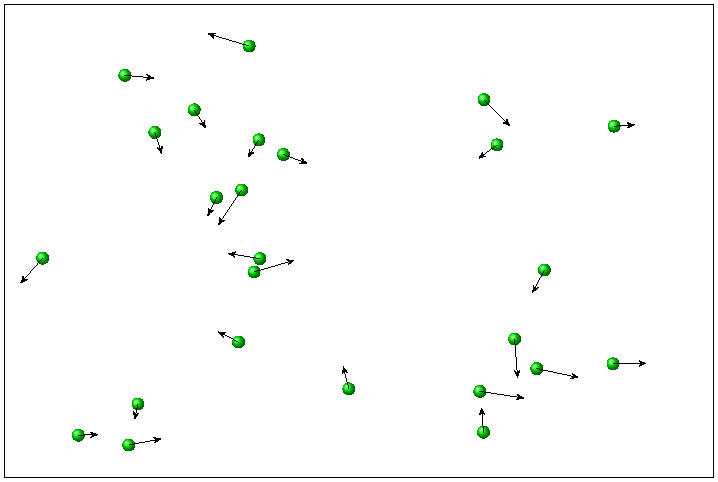
\includegraphics[width=6cm]{gas-random-motion}
		
	motion of gas molecules in a container
	
\end{marginfigure}

gas consists of a large number of molecules

gas molecules move \emph{randomly} at high speeds

\cmt randomness results from \emph{collisions} of fast-moving molecules in the gas

for an individual molecule, its velocity changes constantly as it collides with other molecules

for the gas at any instant, there is a range of velocities for molecules

\cmt experimental evidence of random motion: \keypoint{Brownian motion}\index{Brownian motion}

dust or smoke particles in air undergo jerky random motion (viewed through microscope)

this is due to collisions with gas molecules that move randomly

\cmt speed of gas molecules depend on temperature

molecules move faster at higher temperature\footnote{We will prove this statement later in this chapter.}


\subsection{amount of molecules}

there are a huge number of molecules in a gas

we introduce \keypoint{amount of substance}\index{amount of substance} to measure the size of a collection of particles

\cmt unit of amount of substance: $[n] = \text{mol}$

\begin{ilight}
	one \keypoint{mole} is defined as the amount carbon-12 atoms in a sample of 12 grams
\end{ilight}

\cmt 1 mole of substance contains 6.02$\times$10$^{23}$ particles

this number is called \keypoint{Avogadro constant}\index{Avogadro constant}: $N_A = 6.02\times10^{23} \text{ mol}^{-1}$ \footnote{In 2018, IUPAC suggested a new definition of the mole, which is defined to contain exactly 6.02$\times$10$^{23}$ particles. This new definition fixed numerical value of the Avogadro constant, and emphasized that the quantity `amount of substance' is concerned with counting number of particles rather than measuring the mass of a sample.}

conversion between number of molecules and amount of substance: $\boxed{N=nN_A}$

\cmt it is useful to introduce the notion of molar mass $M$

\begin{ilight}
	\keypoint{molar mass}\index{molar mass} of a substance is defined as the mass of a given sample divided by the amount of substance: $M=\frac{m}{n}$
\end{ilight}

\begin{compactitem}
	\item[--] $\text{amount of substance} = \frac{\text{mass of sample}}{\text{molar mass}}$, or $n = \frac{m}{M}$
	
	\eqyskip
	
	\item[--] $\text{mass of single molecule} = \frac{\text{molar mass}}{\text{Avogadro constant}}$, or $m_0 = \frac{M}{N_A}$
\end{compactitem}

\example{Find the number of molecules in 160 grams of argon-40 gas.}

\sol amount of gas: $n=\frac{m}{M} = \frac{160 \text{ g}}{40 \text{ g mol}^{-1}} = 4.0 \text{ mol}$

number of gas molecules: $N = n N_A = 4.0 \text{ mol} \times 6.02\times10^{23} \text{ mol}^{-1} \approx 2.41 \times 10^{24}$ \eoe

\question{Find the mass of a sample of uranium-235 that contains $6.0\times10^{20}$ atoms.}
	




\subsection{pressure (qualitative view)}

when gas molecules collide with walls of container and rebound, they are acted by a force

by Newton's third law, gas molecules must exert a reaction force on container in return

contributions from many molecules give rise to a pressure

\example{If a gas is heated with its volume fixed, how does the pressure change?}

\sol at higher temperature, gas molecules move faster

they will collide \emph{harder} and produce a greater force upon each collision

they will also collide more \emph{frequently} with the container

so pressure of the gas will increase \eoe

\question{If you pump gas into a bicycle tyre, state and explain how the pressure changes.}

\question{A fixed amount of gas is allowed to expand at constant temperature, state and explain how the pressure changes.}



\subsection{ideal gas}

\subsection{ideal gas equation}

\rcyskip

\begin{ilight}
	a gas that satisfies the equation $\boxed{pV=nRT}$ or $\boxed{pV=NkT}$ at any pressure $p$, any volume $V$, and thermodynamic temperature $T$ is called an \keypoint{ideal gas}\index{ideal gas}
\end{ilight}

\keypoint{molar gas constant}: $R=8.31 \text{ J mol}^{-1}\text{ K}^{-1}$

\keypoint{Boltzmann constant}: $k=1.38\times10^{-23} \text{ J K}^{-1}$

values of $R$ and $k$ apply for any ideal gas, i.e., they are \emph{universal} constants

\cmt recall conversion between number of molecules and amount of substance: $\boxed{N=nN_A}$

we have relation between the constants: $R = kN_A$, or $k=\frac{R}{N_A}$

\cmt one must use \emph{thermodynamic temperature} in the equation

thermodynamic temperature is measured in kelvins (K), so it is also called the \emph{Kelvin scale}\footnote{We will discuss in details about Kelvin scale in \S\ref{s-temp-scale} and \S\ref{s-abs-zero}.}

conversion between Kelvin temperature and Celsius temperature: $\boxed{T_K (\text{K}) \text{ } \autorightleftharpoons{\footnotesize -273}{\footnotesize +273} \text{ } T_C (\OC)}$

\subsection*{real gases}

real gas behaves ideally at sufficiently high temperature and low pressure

\begin{compactitem}
	\item[--] at very low temperatures, real gas will condense into liquid or solid
	
	\item[--] at very high pressures, intermolecular forces become important
\end{compactitem}

however, under normal conditions (room temperature $T \approx 300 \text{ K}$ and standard atmospheric pressure $p \approx 1.0\times10^5 \text{ Pa}$), there is no significant difference between a real gas and an ideal gas

so ideal gas approximation can be used with good accuracy for most of our applications

\example{A sealed cylinder of volume of 0.050 m$^3$ contains 75 g of air. The molar mass of air is 29 g mol$^{-1}$. (a) Find the air pressure when its temperature is $30^\circ$C. (b) The gas is allowed to expand with its pressure fixed. Find the temperature of the gas when the volume doubles.}

\sol amount of gas: $n=\frac{m}{M} = \frac{75}{29} \approx 2.59 \text{ mol}$

\eqyskip

pressure at $30^\circ$C: $p = \frac{nRT_1}{V_1} = \frac{2.59\times8.31\times(30+273)}{0.050} \approx 1.30\times10^5 \text{ Pa}$

\eqyskip

pressure fixed, so $V \propto T \RA \frac{T_2}{T_1} = \frac{V_2}{V_1} = 2 \RA T_2 = 2\times (30+273) = 606 \text{ K} = 333^\circ\text{C}$ \eoe

\example{A gas cylinder holding 5000 cm$^3$ of air at a temperature of 27 $^\circ$C and a pressure of $6.0\times10^5 \text{ Pa}$ is used to fill balloons. Each balloon contains 1000 cm$^3$ of air at 27 $^\circ$C and $1.0\times10^5$ Pa when filled. (a) Find the initial amount of gas in the cylinder. (b) Find the number of balloons that can be filled.}

\sol initial amount of gas in cylinder: $n_0 = \frac{p_0 V}{RT} = \frac{9.0\times10^5\times5000\times10^{-6}}{8.31\times(27+273)} \approx 1.203 \text{ mol}$

\eqyskip

final amount of gas in cylinder: $n_\text{remain} = \frac{pV}{RT} = \frac{1.0\times10^5\times5000\times10^{-6}}{8.31\times(27+273)} \approx 0.201 \text{ mol}$\footnote{Air will leave the cylinder to fill balloons only if pressure inside the cylinder is higher than pressure of the balloon. When the two pressures become equal, no more balloons can be filled, there will be some air remain in cylinder.}

\eqyskip

amount of gas in each balloon: $n_\text{b} = \frac{pV_b}{RT} = \frac{1.0\times10^5\times1000\times10^{-6}}{8.31\times(27+273)} \approx 0.040 \text{ mol}$

\eqyskip

number of balloons: $N = \frac{n_0 - n_\text{remain}}{n_\text{b}} = \frac{1.203-0.201}{0.040} \approx 25$ \eoe

\example{A storage cylinder has a volume of $5.0\times10^{-4}\text{ m}^3$. The gas is at a temperature
	of 300 K and a pressure of $4.0 \times 10^6$ Pa.	(a) Find the number of molecules in the cylinder. (b) The gas molecules slowly leak from the cylinder at a rate of $1.6 \times 10^{16} \text{ s}^{-1}$. Find the time, in days, after which the pressure will reduce by 5.0\%.}

\sol initial number of molecules: $N_0 = \frac{p_0V}{kT} = \frac{4.0\times10^6\times 5.0\times10^{-4}}{1.38\times10^{-23}\times300}\approx 4.83\times10^{23}$

\eqyskip

volume fixed, so $N \propto p \RA \frac{\Delta N}{N_0} = \frac{\Delta p}{p_0} = 5.0\%$

number of molecules escaped: $\Delta N = 0.05\times4.83\times10^{23} \approx 2.42 \times10^{22}$

time needed: $t = \frac{2.42 \times10^{22}}{1.6 \times 10^{16}} \approx 1.51 \times 10^6 \text{ s} \approx 17.4 \text{ days}$ \eoe

\newpage %%%%

\question{Containers $A$ has a volume of $2.5\times10^{-2} \text{ m}^3$ contains a gas at a temperature of 17$^\circ$C and pressure of $1.3 \times 10^5 \text{ Pa}$ and . Another container $B$ of same size holds a gas at same temperature and a pressure of $1.9 \times 10^5 \text{ Pa}$. The two containers are initially isolated from each another. (a) Find the total amount of molecules. (b) The two containers are now connected through a tube of negligible volume. Assume the temperature stays unchanged, find the final pressure of the gas.}

\question{The air in a car tyre can be assumed to have a constant volume of $3.0\times10^{-2} \text{ m}^3$}. The pressure of this air is $2.8\times10^5 \text{ Pa}$ at a temperature of $25^\circ$C. The pressure is to be increased using a pump. On each stroke 0.015 mol of air is forced into the tyre. If gas has a final pressure of $3.6\times10^5 \text{ Pa}$ and final temperature of $28^\circ$C. Find the number of strokes of the pump required.


\subsection{empirical laws}

historically, the ideal gas law was first stated by \emph{\'Emile Clapeyron} in 1834:

for a fixed amount of gas, $\boxed{\frac{PV}{T} = \text{const}}$

his work was based on the empirical Boyle's law, Charles's law, and Gay-Lussac's law

we will next recover these laws from the ideal gas equation

\subsection*{Boyle's law}\index{Boyle's law}

Boyle's law was discovered by \emph{Robert Boyle} in 1662, based on experimental observations

\begin{marginfigure}
	\centering
	\vspace*{-10pt}
		\begin{tikzpicture}[yscale=1.2]
		\draw [thick, <->] (0,4) node[left]{$p$} -- (0,0) node[below]{$0$} -- (4,0) node[below]{$V$};
		\draw [very thick,blue,domain=0.28:3.6,samples=20,smooth,variable=\x] plot (\x,{1/\x)});
		\draw (2.5,2) node{$pV=\text{const}$};
		\end{tikzpicture}
		\vspace*{-10pt}
\end{marginfigure}

if temperature $T$ remains constant, then

{

\centering

$\boxed{pV=\text{const}}$, or $\boxed{p \propto \frac{1}{V}}$

} 

pressure $p$ of gas is inversely proportional to volume $V$

\cmt for a gas with fixed temperature: $p_1 V_1 = p_2 V_2$

\cmt a thermodynamic process for which temperature is kept constant is called an \emph{isothermal} process

$p$-$V$ relation for an isothermal process is shown




\subsection*{Charles's law}\index{Charles's law}

Charles's law was discovered by \emph{Jacques Charles} in 1787, based on experimental observations

\begin{figure}[ht]
	\centering
	\begin{tikzpicture}[scale=1.6]
		\draw [thick, ->] (-2.73,0.6) -- (-2.73,3) node[left]{$V$};
		\draw [thick, ->] (-3.2,0) -- (3,0) node[below]{$T_K/\text{K}$} node[above]{$T_C/\OC$};
		\draw [thick,blue,domain=-0.5:2.8,samples=2,smooth,variable=\x] plot (\x,{0.45*(\x+2.73)});
		\draw [thick,blue,dotted,domain=-2.73:-0.5,samples=2,smooth,variable=\x] plot (\x,{0.45*(\x+2.73)});
		\draw [thick,blue] (-0.5,1.0035) to [out=204.2,in=30] (-1.2,0.65) to [out=210,in=90] (-1.5,0.15);
		\draw[white,fill] (-2.3,0.2) rectangle (-1.8,0.5);
		\foreach \s in {-200,-100,...,200}
		\draw [thick] (\s/100,0) --(\s/100,0.1) node[above]{\s};
		\foreach \s in {0,100,...,500}
		\draw [thick] (\s/100-2.73,0) -- (\s/100-2.73,-0.1) node[below]{\s};
		\draw [thick] (-2.73,0) -- (-2.73,0.1) node[above]{-273};
		\draw [<-, thick] (-1.6,0.6) to [out=90, in=270] (-1,1.6) node[above]{ideal behaviour};
	\end{tikzpicture}
\end{figure}

if pressure $p$ remains constant, then: $\boxed{\frac{V}{T}=\text{const}}$, or $\boxed{V \propto T}$

i.e., volume $V$ of gas is directly proportional to its temperature $T$

\cmt proportionality relation only applies if Kelvin scale is used

\cmt a thermodynamic process for which pressure is kept constant is called an \emph{isobaric} process

$V$-$T$ relation for an isobaric process is shown

\cmt Charles's law implies that volume of gas tends to zero at a certain temperature

historically this is how the idea of \emph{absolute zero} first arose

\cmt as $T\to0$, a real gas condenses into solid

there will be deviation from ideal behaviour (dotted line)



\subsection*{Gay-Lussac's law}\index{Gay-Lussac's law}

\begin{marginfigure}
	\begin{tikzpicture}
		\draw[->](0,0) -- (10,0) node[anchor=north] {$T$C};
		\draw[->](8,-0.2) -- (8,5) node[anchor=west] {$P$};
		\draw[thick, red, dashed] (1,0) -- (8,3.0975);
		\draw[thick, red] (8,3.0975) -- (9.7,3.85);
		\draw (8.1,3.175) node[color=blue] {x};
		\draw (8.4,3.25) node[color=blue] {x};
		\draw (8.7,3.4) node[color=blue] {x};
		\draw (9.0,3.5) node[color=blue] {x};
		\draw (9.3,3.65) node[color=blue] {x};
		\draw (9.6,3.75) node[color=blue] {x};
		\draw[->] (1,-1) node[anchor=north]{Absolute Zero} -- (1,-0.2);
		\end{tikzpicture}
		\caption{Pressure against Temperature of a Gas}
\end{marginfigure}

Gay-Lussac's law was discovered by \emph{Joseph Louis Gay-Lussac} between 1800 and 1802


if volume $V$ remains constant, then

{
	
	\centering
	
	$\boxed{\frac{p}{T}=\text{const}}$, or $\boxed{p \propto T}$
	
} 

i.e., pressure $p$ is directly proportional to temperature $T$

\cmt a thermodynamic process for which volume is kept constant is called an \emph{isochoric} process, or \emph{isometric} process

$p$-$T$ relation for an isochoric process is shown

\cmt behaviour of real gas again deviates from ideal behaviour (dotted line) as $T\to0$





\subsection{kinetic theory of ideal gases}

\keypoint{kinetic model of gases}\index{kinetic model of gases}: a theory based on microscopic motion of molecules of a gas that explains its macroscopic properties

\subsection{assumptions of ideal gas model}

\rcyskip

\begin{ilight}
	
kinetic theory of the ideal gas model is based on the following assumptions:

\begin{compactitem}
	
\item[--] gas molecules are in constant \emph{random} motion
	
\item[--] \emph{intermolecular separation} is much greater than size of molecules

volume of molecules is negligible compared to volume occupied by gas

\item[--] \emph{intermolecular forces} are negligible

\item[--] collisions between molecules are perfectly \emph{elastic}, i.e., no kinetic energy lost

\item[--] molecules travel in straight line between collisions
\end{compactitem}

\end{ilight}

\example{A mass of 20 g helium-4 at a temperature of 37$^\circ$C has a pressure of $1.2\times10^5 \text{ Pa}$. Each helium-4 atom has a diameter of 280 pm. (a) Find the volume occupied by the gas and the volume of atoms in this gas. (b) Compare the two volumes, suggest whether this gas can be considered as an ideal gas.}

\sol number of helium molecules: $N = nN_A = \frac{m}{M} \times N_A = \frac{20}{4.0} \times 6.02\times10^{23} \approx 3.01\times10^{24} $

\eqyskip

volume of gas: $V_\text{gas} = \frac{NkT}{p} = \frac{3.01\times10^{24}\times1.38\times10^{-23}\times (37+273)}{1.2\times10^5} \approx 0.107 \text{ m}^3$

\eqyskip

volume of one atom: $V_\text{atom} = \frac{4}{3}\pi r^3 = \frac{4}{3} \pi\times(140\times10^{-12})^3 \approx 1.15\times10^{-29} \text{ m}^3$

volume of all atoms: $V_\text{atoms} = N V_\text{atom} = 3.01\times10^{24} \times 1.15\times10^{-29} \text{ m}^3 \approx 3.46 \times 10^{-5} \text{ m}^{3}$

$V_\text{gas} \gg V_\text{atoms}$, so this gas can approximate to an ideal gas \eoe


\subsection{pressure (quantitative view)}

we are ready to derive a formula for pressure due to ideal gas

pressure of gas is due to collision of gas molecules with container

let's first consider the effect of one single molecule moving in one dimension only, and then generalise the result to a gas containing $N$ molecules moving in all three dimensions



\begin{figure}[ht]
\centering
\begin{tikzpicture}[scale=1]
\coordinate (A) at (0,0); 
\coordinate (B) at (3,0);
\coordinate (C) at (4.5,1); 
\coordinate (D) at (1.5,1);
\coordinate (E) at (0,3); 
\coordinate (F) at (3,3);
\coordinate (G) at (4.5,4); 
\coordinate (H) at (1.5,4);
\draw [gray!20,fill] (A) -- (D) -- (H) -- (E) -- cycle;
\draw [thick] (B) -- (A) -- (E) -- (F) -- (B) -- (C) -- (G) -- (H) -- (E);
\draw [thick] (F) -- (G);
\draw [thick,dashed] (A) -- (D) -- (C);
\draw [thick,dashed] (D) -- (H);
\draw [thick,blue,->] (1.6,2.1) -- (0.9,2.1) to [out=180,in=90] (0.75,1.95)to [out=-90,in=180] (0.9,1.8) -- (2.4,1.8) node[below, pos=0.7]{$v$};
\shade [ball color = green] (1.8,2.1) circle [radius=0.1];
\draw [thick,<->] (0,-0.5) -- (1.5,-0.5) node[below]{$l$} -- (3,-0.5);
\node at (0.75,2.5) {{\Large $A$}};
\node[above] at (1.8,2.2) {{\footnotesize $m$}};
\end{tikzpicture}

one gas molecule moving in 1-D
\end{figure}

let's assume this single molecule only moves in $x$-direction (see figure)

change in momentum when colliding with wall: $\Delta P_x = mv_x - (-mv_x) = 2mv_x$\footnote{In this chapter we use $P$ for momentum of a particle and $p$ for pressure of a gas to avoid confusion.}

time interval between collisions: $\Delta t=\frac{2l}{v_x}$

average force acting: $F_x=\frac{\Delta P_x}{\Delta t} = \frac{2mv_x}{\tfrac{2l}{v_x}} = \frac{mv_x^2}{l}$

average pressure: $p_x=\frac{F}{A} = \frac{mv_x^2}{lA} = \RA p_x = \frac{mv_x^2}{V}$

generalisation to $N$ molecules moving in 3-D

\begin{compactitem}
	\item[--] $N$ molecules so $N$ times the contributions to pressure
	
	but there is a \emph{distribution} of speeds for $N$ molecules, so should take average of $v^2$
	
	\item[--] in three-dimensional space, we have: $v^2=v_x^2 + v_y^2 + v_z^2$
	
	but molecules have no preference in any specific direction, so: $\avg{v_x^2} = \avg{v_y^2} = \avg{v_z^2} = \frac{\avg{v^2}}{3}$
	
	pressure should be shared equally among three dimensions: $p=p_x=p_y=p_z$
		
\end{compactitem}


therefore we find the pressure of an ideal gas is given by: $\boxed{p = \frac{Nm\avg{v^2}}{3V}}$

\cmt $\avg{v^2}$ is the \emph{mean square velocity} of gas molecules

we can further define r.m.s. (root mean square) velocity: $v_\text{rms} = \sqrt{\avg{v^2}}$ 

gas molecules in random motion so there exists a range of velocities

we cannot tell exact velocity of a specific molecule, but can only tell mean values

\cmt $N$ is number of molecules, $m$ is mass of one molecule

then $Nm$ gives total mass of the gas, and $\frac{Nm}{V}$ gives gas density $\rho$

we can rewrite the pressure formula as: $\boxed{p=\frac{1}{3}\rho \avg{v^2}}$ 

(pressure depends only on density and mean square speed of molecules)

\cmt physical interpretation of the formula

\begin{compactitem}
\item[--] $N \up$ $\ra$ more molecules, more collisions $\ra p\up$

\item[--] $m \up$ $\ra$ greater mass, greater force upon collision $\ra p\up$

\item[--] $v \up$ $\ra$ strike container harder, also more often $\ra p\up$

\item[--] $V \up$ $\ra$ spend more time in gas, less frequent collision with container $\ra p\down$
\end{compactitem}


\subsection{kinetic energy}

we now have two equations for ideal gases:
\begin{equation*}
\left\{
	\begin{array}{ll}
	pV = nRT \, \text{, or } \, pV = NkT &\quad \text{ideal gas law} \\
	p = \frac{Nm\avg{v^2}}{3V} &\quad \text{pressure law}
	\end{array} \right.
\end{equation*}

compare the two equations: $pV=\frac{1}{3}Nm\avg{v^2}=NkT \RA m\avg{v^2}=3kT$

\emph{mean kinetic energy} of a single molecule in a gas is: $\boxed{\avg{E_k}=\frac{1}{2}m\avg{v^2}=\frac{3}{2}kT}$

mean K.E. of ideal gas molecules is \emph{proportional} to its thermodynamic temperature

\cmt useful relation for molecular speeds: $\boxed{v_\text{rms}^2 \propto T}$

recall our statement in \S\ref{s-gas-intro}, higher temperature means higher speed for molecules

\cmt we only talk about \emph{translational} K.E. here

molecules have this energy because they are moving through space

total kinetic energy may also include \emph{rotational} K.E. and \emph{vibrational} K.E.
\footnote{There is an important result in classical thermal physics, known as the \emph{equipartition of energy theorem}. It states that the average energy per molecule is $\frac{1}{2}kT$ for each independent \emph{degree of freedom}. A molecule can move in three directions, corresponding to three translational degrees of freedom, thus its mean translational kinetic energy is $\frac{3}{2}kT$. For a polyatomic gas (each molecule consists of several atoms), apart from translational motion , it has additional rotational degrees of freedom and different vibrational modes, so its average energy can be calculated by counting the total number of degrees of freedom.}

\cmt $\avg{E_k} = \frac{3}{2}k T$ gives the \emph{mean}, or \emph{average} K.E. per molecule

gas molecules exchange energies with each other upon collisions

for an individual molecule, its K.E. is not a constant

but mean K.E. is constant, which depends on temperature $T$ only

\cmt in a mixture of several gases, K.E. is shared \emph{equally} among its components

this is because of repeated collisions between particles

though all molecules have same K.E., heavier molecules will move more slowly




\example{Air consists of oxygen (O$_2$, molar mass $32\text{ g mol}^{-1}$) and nitrogen (N$_2$, molar mass $28\text{ g mol}^{-1}$). (a) Calculate the mean translational kinetic energy of these molecules at 300 K. (b) Estimate the typical speed for each type of the molecule.}

\sol mean K.E. of single molecule: $\avg{E_k} = \frac{3}{2}kT = \frac{3}{2} \times 1.38\times10^{-23} \times 300 \approx 6.21\times 10^{-21} \text{ J}$

{
	
	\centering
	
	$\avg{E_k} = \frac{1}{2}m\avg{v^2} = \frac{3}{2} kT \RA \frac{1}{2} \frac{M}{N_A} \avg{v^2} = \frac{3}{2} kT \RA \avg{v^2} = \frac{3kN_AT}{M} = \frac{3RT}{M}$
	
}

\eqyskip

for oxygen molecule: $v_\text{O$_2$} \approx  \sqrt{\frac{3\times8.31\times300}{0.032}} \approx 483 \mps$

\eqyskip

for nitrogen molecule: $v_\text{N$_2$} \approx  \sqrt{\frac{3\times8.31\times300}{0.028}} \approx 517 \mps$ \eoe

\example{A cylinder container initially holds a gas of helium-4 at a temperature of 54\OC. (a) Find the mean square speed of these helium atoms. (b) If the temperature is raised to 540\OC, find the r.m.s. speed of the atoms.}

\sol mass of one helium-4 atom: $m=4\text{u} = 4\times 1.66\times10^{-27} \approx 6.64\times10^{-27} \text{ kg}$

at 54\OC: $\, \frac{1}{2}m\avg{v^2} = \frac{3}{2}kT \RA \avg{v^2} = \frac{3kT}{m} = \frac{3\times1.38\times10^{-23}\times(54+273)}{6.64\times10^{-27}} \approx 2.04 \times 10^6 \text{ m}^2 \text{ s}^{-2}$

\eqyskip 

note relation between $v$ and $T$: $\, \avg{v^2} \propto T \RA \frac{\avg{v^{\prime 2}}}{\avg{v^2}} = \frac{T'}{T} \RA v'_\text{rms} = \sqrt{\frac{T'}{T}}\times v_\text{rms}$

\eqyskip 

at 540\OC: $\, v'_\text{rms} = \sqrt{\frac{540+273}{54+273}} \times \sqrt{2.04 \times 10^6} \approx 2.25 \times 10^3 \mps$ \eoe


\question{A fixed mass of gas expands to twice its volume at constant temperature. (a) How does its pressure change? (b) How does mean kinetic energy change?}

\question{In order for a molecule to escape from the gravitational field of the earth, it must have a speed of $1.1\times10^6\mps$ at the top of the atmosphere. (a) Estimate the temperature at which helium-4 atoms could have this speed. (b) Helium atom actually escape from top of the atmosphere at much lower temperatures, explain how this is possible.}
% \chapter{Thermodynamics}


\subsection{thermal physics basics}


\subsection{temperature scales}\label{s-temp-scale}

\begin{marginfigure}
	\centering
	\vspace*{-2.7cm}
	\begin{tikzpicture}[yscale=1.6]
	\draw[->] (0,-3) -- (0,1.50);
	\foreach \temp in {-2.73,-1.96,0,0.25,1.00} \draw (-0.1,\temp) --++ (0.2,0);
	\node[left] at (-0.2,1.5) {$T_C(\OC)$};
	\node[right] at (0.2,1.5) {$T_K(\text{K})$};
	\node[left] at (-0.2,-2.73) {-273\OC};
	\node[left] at (-0.2,-1.96) {-196\OC};
	\node[left] at (-0.2,-0) {0\OC};
	\node[left] at (-0.2,0.25) {25\OC};
	\node[left] at (-0.2,1) {100\OC};
	\node[right] at (0.2,-2.73) {0 K};
	\node[right] at (0.2,-1.96) {77 K};
	\node[right] at (0.2,-0) {273 K};
	\node[right] at (0.2,0.25) {298 K};
	\node[right] at (0.2,1) {373 K};
	\node[right] at (1.35,-2.73) {absolute zero};
	\node[right] at (1.35,-1.96) {liquid nitrogen};
	\node[right] at (1.35,0) {ice-water mixture};
	\node[right] at (1.35,0.25) {room temperature};
	\node[right] at (1.35,1.00) {boilng water};
	\end{tikzpicture}
	\vspace*{-30pt}
\end{marginfigure}

\cmt Celsius scale (unit: \OC)

0$^\circ$C defined as temperature of ice-water mixture

100$^\circ$C defined as temperature of boiling water

\cmt Kelvin scale (unit: K)

0 K (\emph{absolute zero}) is lowest temperature possible

\cmt conversion rule: $T_K (\text{K}) \text{ } \autorightleftharpoons{\footnotesize -273}{\footnotesize +273} \text{ } T_C (\OC)$

\cmt change of 1$^\circ$C equals change of 1 K


\subsection{kinetic theory of matter}

there are three common states of matter: solid, liquid and gas

they have very different physical properties (density, compressibility, fluidity, etc.)

but deep down, they are all composed of a large number of small molecules

in the \keypoint{kinetic theory of matter}, we look at microscopic behaviour at molecular level (arrangement, motion, intermolecular forces, separation, etc.)

\emph{microscopic} behaviour of molecules cause differences in \emph{macroscopic} properties of matter

\begin{compactitem}
	\item[--] solid: molecules close together, tightly bonded, vibrate about their positions
	
	\item[--] liquid: molecules quite close together, vibrate but has some freedom to move about
	
	\item[--] gas: molecules widely separated, free from neighbours, move rapidly
\end{compactitem}

\subsection{specific latent heat}

it requires heat energy to \emph{melt} a solid or \emph{boil} a liquid

melting and boiling usually occur at a fixed temperature

thermal energy to cause the change of state at a constant temperature is called \emph{latent heat}

amount of latent heat needed depends on mass of substance: $\boxed{Q=Lm}$

\begin{ilight}
	we define \keypoint{specific latent heat}\index{specific latent heat} ($L$) as the thermal energy required to change the state of \emph{unit} mass of substance with no change in temperature is called 
\end{ilight}



\cmt unit of specific latent heat: $[L] = \text{J}\cdot\text{kg}^{-1}$

\cmt specific latent heat is an \emph{intensive} property

i.e., $L$ does not depend on size or shape of sample, $L$ depends on type of substance only 
	
\cmt for melting, $L$ is called \emph{specific latent heat of fusion}
	
for boiling, $L$ is called \emph{specific latent heat of vaporisation}
	
\cmt latent heat is related to breaking bonds and increasing intermolecular separation
	
vaporisation requires larger increase in particle separation than fusion
	
for a given substance, $L_\text{vapour}>L_\text{fuse}$


\example{A 3.0 kW electric kettle contains 0.5 kg of water already at its boiling point. Neglecting heat losses, determine how long it takes to boil dry. ($L_\text{water} = 2.26 \times 10^6 \text{ J kg}^{-1}$)}
	
\sol heat required: $Q=mL = 0.50 \times 2.26 \times 10^6 = 1.13 \times 10^6 \text{ J}$
	
time needed: $t=\frac{Q}{P} = \frac{1.13 \times 10^6}{3.0\times 10^3} \approx 380 \text{ s} \approx 6.3 \text{ min}$ \eoe
 
\example{A student measures specific latent heat of fusion for ice. He uses an electric heater to melt ice but the insulation is not perfect. The experiment is carried out twice, with the heater operating at different powers. Use the data table to calculate specific latent heat of fusion.}

\begin{center}
	\begin{tabular}{|C{1.6cm}|C{2cm}|c|c|}
		\hline  & Power (W) & time interval (min) & mass of ice melted (g) \\ 
		\hline test 1 & 60 & 3.0 & 40.4 \\ 
		\hline test 2 & 90 & 3.0 & 56.6 \\ 
		\hline 
	\end{tabular} 
\end{center}

\sol there exists heat gain from surroundings, so effective power $P_\text{eff}=P_\text{heater}+P_\text{sur}$

heat energy to melt ice: $Q = mL = (P_\text{heater}+P_\text{sur}) t$
\begin{equation*}
	\left\{ \begin{array}{l}
		40.4 \times L = (60+P_\text{sur})\times3.0\times60 \\
		56.6 \times L = (90+P_\text{sur})\times3.0\times60 
	\end{array}\right.
	\RA \left\{ \begin{array}{l}
	L \approx 333 \text{ J g}^{-1} \\
	P_\text{sur} \approx 14.8 \text{ W} \end{array}\right. 
\end{equation*}

\eqyskip

\question{A student designs an experiment to determine the specific latent heat of fusion $L$ of ice. Some ice at $0\OC$ is heated with an electric heater. The experiment is carried out twice and the following data are obtained.
	
\begin{center}
	\begin{tabular}{|c|c|c|c|}
		\hline  & energy supply from heater (J) & time interval (min) & mass of ice melted (g) \\ 
		\hline heater off & 0 & 10.0 & 14.3 \\ 
		\hline heater on & 21000 & 5.0 & 70.0 \\ 
		\hline 
	\end{tabular} 
\end{center}

(a) Suggest why two sets of readings are taken. (b) Find specific latent heat of fusion for ice.}

\subsection{specific heat capacity}

heating a substance could cause an increase in its temperature

heat required is proportional to its mass $m$ and temperature change $\Delta T$: $\boxed{Q=cm\Delta T}$

\begin{ilight}
	we define \keypoint{specific heat capacity }\index{specific heat capacity} ($c$) as the thermal energy required per unit mass of substance to cause an increase of one unit in its temperature
\end{ilight}


\cmt unit of specific heat capacity: $[c] = \text{J kg}^{-1} \text{ K}^{-1}$ or J kg$^{-1}$ $^\circ\text{C}^{-1}$
	
\cmt $c$ is also an \emph{intensive} property, i.e., independent of size or shape of the sample


\example{A block of 30 g ice at $-20^\circ$C is added to a large cup of 270 g water at 80$^\circ$C. Assume there is no energy lost, what is the final temperature of the mixture? (data: specific heat capacity of water is 4200 J kg$^{-1}$ K$^{-1}$, specific heat capacity of ice is 2100 J kg$^{-1}$ K$^{-1}$, specific latent heat of ice is $3.3\times10^5$ J kg$^{-1}$.}

\sol energy lost by hot water = energy gain by ice cube
\begin{equation*}
	\underbrace{4200\times0.27\times(80-T)}_{\text{95 $^\circ\text{C}$ water $\to T$ $^\circ\text{C}$  water}} = 
	\underbrace{2100\times0.030\times[0-(-20)]}_{-\text{20 $^\circ\text{C}$ ice $\to 0$ $^\circ\text{C}$  ice}} +
	\underbrace{3.3\times10^5\times0.030}_{\text{0 $^\circ\text{C}$ ice $\to 0$ $^\circ\text{C}$ water}} + 
	\underbrace{4200\times0.030\times(T-0)}_{\text{0 $^\circ\text{C}$ water $\to T$ $^\circ\text{C}$  water}}
\end{equation*}

\vspace*{-1em}
\begin{equation*}
	90720 - 1134T = 1260 + 9900 + 126 T
\end{equation*}
\begin{equation*}
	T = \frac{90720-1260-9900}{1134+126} \approx 63 ^\circ\text{C} 
\end{equation*}


\example{A 1.00 kg aluminium block is heated using an electrical heater. The current in the heater is 4.2 A and the p.d. across is 12 V. Measurements of the rising temperature are represented by the graph. Determine specific heat capacity  of aluminium.}

\begin{figure}[ht]
	\centering
	\begin{tikzpicture}[scale=1]
	\draw[style=help lines,step=0.5,gray!50] (0,0) grid (7.5,5.5);
	\draw [thick, ->] (-0.5,0) --(8,0) node[below]{$t/\text{s}$};
	\draw [thick, ->] (0,-0.5) --(0,6) node[left]{$T/\OC$};
	\foreach \s in {100,200,...,700}
	\draw [very thick] (\s/100,-0.1) -- (\s/100,0) node[below]{\s} -- (\s/100,0.1);
	\foreach \s in {10,20,...,50}
	\draw [very thick] (-0.1,\s/10) -- (0,\s/10) node[left]{\s} -- (0.1,\s/10);
	\draw [very thick,blue] (0,2) -- (7.5,5.075);
	\draw [very thick,red] (0,2) -- (5.5,2) node[midway,below]{\textcolor{black}{$\Delta t = 550 \text{ s}$}} -- (5.5,4.255) node[right,midway]{\textcolor{black}{$\Delta T = 22.5 \OC$}};
	\foreach \s in {0,1,...,7}
	\draw [fill] (\s,2+0.41*\s) circle(0.05);
	\end{tikzpicture}
\end{figure}

\sol energy supplied: $Q = cm\Delta T \RA IV\Delta t = cm\Delta T \RA c = \frac{IV}{m \tfrac{\Delta T}{\Delta t}} $

$\frac{\Delta T}{\Delta t}$ is gradient of fitting line: $\frac{\Delta T}{\Delta t} = \frac{22.5}{550} \approx 4.09 \times 10^{-2} \text{ } \OC \text{ s}^{-1}$

specific heat capacity: $c = \frac{4.2\times12}{1.00 \times 4.09 \times 10^{-2}} \approx 1230 \jpkgC$	\eoe

\question{A mixture contains 5\% silver and 95\% of gold by weight. Some gold is melted and the correct weight of silver is added. The initial temperature of silver is $20^\circ$C. Use the data to calculate the initial temperature of gold so that the final mixture is at melting point of gold.}

\begin{center}
	\begin{tabular}{|l|c|c|}
		\hline  & silver & gold \\ 
		\hline melting point (K) & 1240 & 1340 \\ 
		\hline specific heat capacity (solid or liquid) (J kg$^{-1}$ K$^{-1}$) & 235 & 129 \\ 
		\hline specific latent heat of fusion (kJ kg$^{-1}$) & 105 & 628 \\
		\hline 
	\end{tabular} 
\end{center}



\subsection{internal energy}

we now consider the total energy within a thermodynamic system

molecules in a system undergo random motion, so they have kinetic energy

there are potential energy between molecules due to intermolecular interaction

\begin{ilight}
	\keypoint{internal energy}\index{internal energy} is defined as the sum of random kinetic energy of molecules and potential energy between molecules: $\boxed{U=E_k+E_p}$
\end{ilight}

\cmt internal energy is a \emph{state function} of the system

it only depends on current state of system, not on process to arrive at this state

\subsection{kinetic energy}

\cmt internal energy counts K.E. due to random motion at molecular level

K.E. of macroscopic motion of the system as a whole is not included

\cmt mean K.E. of molecules is directly proportional to temperature: $\boxed{E_k \propto T}$

K.E. of molecules depends on temperature only

higher temperature means molecules move faster, vibrate more intensively, etc.





\subsection{potential energy}

\cmt internal energy counts P.E. due to force fields \emph{within} the system

P.E. of the system as a whole due to \emph{external} force fields is not included

\cmt P.E. between molecules depends on intermolecular separation and chemical bonding

in general, greater intermolecular separation means greater P.E.\footnote{Intermolecular separation does not necessarily increase during melting processes. A typical counter example is melting of ice into water, for which intermolecular separation actually decreases (density of water > density of ice), but potential energy of the system will still increase because hydrogen bonds between H$_2$O molecules are broken.}: $\boxed{r \up \Leftarrow E_p \up}$

breaking intermolecular bonds also causes an increase in P.E.

mean P.E. of gas $>$ mean P.E. of liquid $>$ mean P.E. of liquid solid

\subsection{internal energy of ideal gas}

for ideal gas, mean K.E. of one molecule: $E_k = \frac{3}{2}kT$

there is no intermolecular force, so P.E. of ideal gas is defined to be zero: $E_p = 0$

internal energy per molecule: $U = E_k + E_p = \frac{3}{2}kT$

hence internal energy of ideal gas is purely kinetic and directly proportional to temperature

total internal energy of the gas: $U_\text{gas} = NU \RA \boxed{U_\text{gas} = \frac{3}{2}NkT}$

\subsection{change of states}

consider a substance being heated from its solid state

it will melt into a liquid and further vaporise into its gaseous state

we now look into the changes of internal energy during each stage

\begin{figure}[ht]
\centering
\begin{tikzpicture}[scale=1]
\draw[thick,->] (-1,-2) -- (0,-2) -- (10,-2) node[below] {$t$};
\draw[thick,->] (0,-2.5) -- (0,5) node[left]{$T$};
\draw [very thick,blue] (0,-1) node[left]{$A$} -- (1,0) node[above]{$B$} -- (2.5,0) node[above left]{$C$} -- (4,3) node[above]{$D$} -- (9,3) node[above left]{$E$} -- (9.5,4.5) node[above]{$F$};
\draw[thick,dashed] (4,3) -- (0,3) node[left]{$T_\text{boiling}$};
\draw[thick,dashed] (1,0) -- (0,0) node[left]{$T_\text{melting}$};
\end{tikzpicture}
\end{figure}


\begin{compactitem}
\item[--] $AB$ (solid state): $T \up \ra E_k \up$, greater vibration for solid particles

but no (significant) change in mean separation\footnote{A typical solid material expands when it is heated, so intermolecular separation will increase slightly.} $\ra$ no change in P.E.

\item[--] $BC$ (\emph{melting}): latent heat goes into breaking intermolecular bonds, $r\up \ra E_p \up$

but melting occurs at constant temperature\footnote{Here we talk about \emph{pure substance}, which changes from solid into liquid at a particular temperature, called the \emph{melting point}. But for a \emph{mixture} of substances, melting may occur over a \emph{range} of temperatures. It is also possible for a substance to decompose before they change states.} $\ra$ no change in K.E.

\item[--] $CD$ (liquid state): $T \up \ra E_k \up$, greater vibration and free motion

but no (significant) change in mean separation $\ra$ no change in P.E.

\item[--] $DE$ (\emph{boiling}): molecules break free, $r\up \ra E_p \up$

boiling occurs at constant temperature\footnote{Again we only concern pure substances. Mixtures that boil over a range of temperatures or substance decompose before phase transition are not considered here.} $\ra$ no change in K.E.

\item[--] $EF$ (gas state): $T \up \ra E_k \up$ particles move even faster

particles completely separated, no intermolecular force, so constant $E_p = 0$
\end{compactitem}

\question{For a particular substance, why is the specific latent heat of vaporisation much greater than the specific latent heat of fusion?}

\subsection*{evaporation}

liquid changes into gas without boiling $\longrightarrow$ \keypoint{evaporation}

particles move randomly, i.e., they move at various speeds

some molecules move fast enough to break free

\cmt \emph{cooling effect}: evaporation causes a decrease in temperature of the liquid

most energetic molecules escaped, those remain in the liquid have less energy, $E_k \down \ra T \down$

\cmt rate of evaporation increases with temperature, surface area of liquid

\cmt different between boiling and evaporation

\begin{center}
	\begin{tabular}{|c|c|c|}
		\hline 
		& boiling & evaporation \\ 
		\hline 
		occurrence & throughout the liquid & at surface only \\ 
		\hline 
		temperature & occur at boiling point & occur at any temperature \\ 
		\hline 
		bubble formation & bubbles formed & no bubbles \\ 
		\hline 
		rate of process & fast & slow \\ 
		\hline 
	\end{tabular} 
\end{center}

\subsection{first law of thermodynamics}

internal energy of a system changes upon heat transfer or doing work

\begin{ilight}
	\keypoint{first law of thermodynamics}\index{law of thermodynamics!first law of thermodynamics} states that the increase in internal energy equals sum of heat supply to the system and work done on the system: $\boxed{\Delta U = Q +  W}$
\end{ilight}

\cmt first law of thermodynamics is an extension of the law of conservation of energy

\cmt sign conventions for $Q$ and $W$

\begin{compactitem}
	\item[$\circ$] $Q>0$ if heat supplied to system
	
	\item[$\circ$] $Q<0$ if heat released by system to surroundings
	
	\item[$\circ$] $W>0$ if work done \emph{on} system by external
	
	i.e., if system is compressed and volume decreases, then $W>0$
	
	\item[$\circ$] $W<0$ if system does work \emph{against} surroundings
	
	i.e., system expands and volume increases, then $W<0$
	
\end{compactitem}

\cmt amount of heat energy: $Q=\left\{ \begin{array}{l}
	cm\Delta T \qquad (\text{if no change of state}) \\
	Lm \qquad (\text{during change of state})
	\end{array}\right.$

\cmt amount of work is related to pressure and change of volume

if volume changed at \emph{constant} pressure, then $W=F\Delta s = pA\Delta s \ra \boxed{W = p\Delta V}$\footnote{If pressure changes with volume during a thermodynamics process, then work done $W=\int p \dd V$. Alternatively, we can evaluate the area under a $p$-$V$ graph to find the work done.}

if no change of volume, then no work is done

\begin{figure}[h]
		\begin{tikzpicture}[domain=1:9]
		\draw[->] (-0.5,0) -- (12,0) node[anchor=north] {$V$};
		\draw[->] (0,-0.5) -- (0,10) node[anchor=east] {$P$};
		\draw (1,9) node[anchor=south]  {\textbf{A}};
		\draw[thick, ->]  (1,9) .. controls (4,7) and (7,6.2) .. (8,6) node[midway, anchor=south west] {\textbf{1}};
		\draw[thick, ->] (8,6) .. controls (9,4.5) and (10,3) .. (12,1) node[anchor=south west, midway] {\textbf{2}};
		\draw[thick, ->] (12,1) .. controls (8,1.5)  .. (3,3) node[midway, anchor=north east] {\textbf{3}};
		\draw[thick, ->] (3,3) .. controls (1.6,6)  .. (1,9) node[midway, anchor=north east] {\textbf{4}};
		\end{tikzpicture}
		\caption{The Carnot Cycle}
		\label{carnotcycle}
	\end{figure}
 
The Carnot Cycle shown in Figure \ref{carnotcycle} is commonly used to test the understanding for the first law. The cycle begins and ends at point \textbf{A}. This means that the internal energy of the system at the start and end of the cycle is the same (as $PV=nRT$ and $T$ is proportional to the internal energy). The changes at each stage of the cycle are as follows:
	
	\begin{description}
		\item[1. Isothermal Expansion] In stage 1 the gas expands at contant temperature. Since it is expanding, the gas is doing work on the surroundings and since it is at constant temperature the internal energy of the gas remains constant. Therefore the second law implies that the gas must be absorbing heat. \emph{Note that isothermal changes are often indicated by describing the change as occuring slowly.}
		\item[2. Adiabatic Expansion] In stage 2 the gas expands without transferring heat to/from the surroundings. Since it is doing work the gas's internal energy drops, as does its temperature.
		\item[3. Isothermal Compression] In stage 3 the gas is compressed at constant temperature. Since work is done on the gas and the internal energy remains constant it must be the case that heat is lost to the surroundings.
		\item[4. Adiabatic Compression] Finally, the gas is compressed without heat transfer to/from the surroundings. Work is done on the gas and therefore the internal energy, and termperature, increase.
	\end{description}
	
	
	\begin{example}
		
		Complete the table for the Carnot Cycle shown in figure \ref{carnotcycle}.
		
		\begin{tabular}{|c|p{3cm}|p{3cm}|p{3cm}|}
			\hline
			stage & \centering thermal energy supplied \textbf{to} the gas / J & \centering work done \textbf{on} the gas / J & \centering \textbf{increase} in internal energy of the gas / J \tabularnewline \hline
			1 & \centering\centering(a) & \centering-936 & \centering(b) \tabularnewline \hline
			2 & \centering0 & \centering(c) & \centering(d) \tabularnewline \hline
			3 & \centering(e) & \centering+702 & \centering0 \tabularnewline \hline
			4 & \centering(f) & \centering+844 & \centering+844 \tabularnewline \hline
		\end{tabular}
		
		
		
		In stage 1 there is no change in internal energy of the gas, so (b) equals zero. In order to satisfy the first law of thermodynamics the thermal energy supplied must equal the work done \textbf{by} the gas so (a) equals +936J.
		
		As the total change in internal energy throughout the cycle must be zero, we can now calculate (d) as being -844J.
		
		(c) can be calculated using the first law as -844J.
		
		A similar argument to that used in stage 1 can be used in stage 3 to give (e) as -702J.
		
		In stage 4 no energy is transferred by heating therefore (f) is equal to zero.
		
		
		
		The final table is therefore:
		
		\begin{tabular}{|c|p{3cm}|p{3cm}|p{3cm}|}
			\hline
			stage & \centering thermal energy supplied \textbf{to} the gas / J & \centering work done \textbf{on} the gas / J & \centering \textbf{increase} in internal energy of the gas / J \tabularnewline \hline
			1 & \centering\centering \textbf{+936} & \centering-936 & \centering \textbf{0} \tabularnewline \hline
			2 & \centering0 & \centering \textbf{-844} & \centering \textbf{-844} \tabularnewline \hline
			3 & \centering \textbf{-702} & \centering+702 & \centering0 \tabularnewline \hline
			4 & \centering \textbf{0} & \centering+844 & \centering+844 \tabularnewline \hline
		\end{tabular}
		
	\end{example} 

\example{A gas is heated by supplying it with 25 kJ of energy. The gas expands so that the volume increases by 0.10 m$^3$. Assume the gas has a fixed pressure of 150 kPa during the process. Calculate the change in internal energy.}

\sol amount of work done: $W = p \Delta V = 150 \times 0.10 = 15 \text{ kJ}$

but gas expands means work is done against surroundings, so this is negative work

change in internal energy: $\Delta U = Q +  W = (+25) + (-15) = +10 \text{ kJ}$ \eoe

\example{Use the idea of internal energy and the first law of thermodynamics, explain why boiling water requires heat supply.}

\sol boiling occurs at constant temperature, so $\Delta E_k = 0$

but separation between molecules increased, so $\Delta E_p >0$

by definition, internal energy $U=E_k+E_p$, so $\Delta U >0$

during boiling, there is an increase in volume, so work against surroundings, $W<0$

recall first law of thermodynamics $\Delta U = Q + W$, must have $Q>0$

this means heat must be supplied for boiling processes \eoe

\example{When you pump up a bicycle tyre, the temperature of air inside the tyre will go up. Explain why this happens using the first law of thermodynamics.}

\sol pumping up tyre involves compressing gas, so positive work is done: $W>0$

for each stroke, there is little time for heat transfer, so $Q \approx 0$

according to first law of thermodynamics $\Delta U = Q + W \RA \Delta U >0$

by definition, internal energy $U=E_k + E_p \RA \Delta U = \Delta E_k + \Delta E_p>0$

but for gas, there is negligible intermolecular force, so $\Delta E_p=0$, then must have $\Delta E_k>0$

K.E. of molecules is proportional to temperature, higher K.E. so higher temperature \eoe

\example{An ideal gas of 0.080 mol is initially at state $A$ and then undergoes a cycle $ABCA$. The variation of its pressure $p$ with its volume $V$ is shown on the graph.}

\begin{figure}[ht]
	\centering
	\begin{tikzpicture}[scale=0.9]
	\draw[<->] (0,7.5) node[left]{$p$/kPa} -- (0,0) -- (7.5,0) node[below] {$V/10^{-2}$ m$^3$};
	\draw[help lines, gray] (0,0) grid (7,7);
	\foreach \x in {0,100,200,300} \node[left] at (-0.1,\x*2/100) {$\x$};
	\foreach \x in {0,2,4,6} \node[below] at (\x,-0.1) {$\x$};
	\draw[very thick, blue, ->] (2,2) node[below left]{$A$} -- (2,4.5);
	\draw[very thick, blue] (2,4.5) -- (2,6) node[above left]{$B$};
	\draw [very thick, blue, domain=2:6] plot (\x, {12/\x}) node[below right]{$C$};
	\draw[very thick, blue, ->] (6,2) -- (3.5,2);
	\draw[very thick, blue] (3.5,2) -- (2,2);
	\draw[very thick, blue, ->] (4.5,2.67) -- (4.55,2.64);
	\end{tikzpicture}
\end{figure}

Temperature of state $A$ is 300 K. The magnitude of work on gas from state $B$ to $C$ is 6570 J.

For each stage $A \to B$, $B \to C$ and $C \to A$ during the cycle, determine work done and heat supply to the gas, and also find the change in internal energy.

\newpage

\sol work done depends on change in volume

$A\to B$: no change in volume, so $W_{AB} = 0$

$B \to C$: $|W_{BC}|= 6570 \text{ J}$, but expansion implies $W<0$, so $W_{BC}=-6570 \text{ J}$

$C \to A$: $|W_{CA}| = p\Delta V_{CA} = 1\times10^5 \times (6-2)\times10^{-2} \RA W_{CA}= +4000 \text{ J}$ (compression so $W>0$)

\noindent change in internal energy of ideal gas depends on change in temperature

$A\to B$: same $V$ but $p_B = 3p_A$, so $T_B = 3T_A = 900 \text{ K}$

$\phantom{A\to B\text{: }}\Delta U_{AB} = \frac{3}{2}Nk\Delta T_{AB} = \frac{3}{2}\times 0.80\times 6.02\times10^{23}\times1.38\times10^{-23}\times(900-300) \approx +5980 \text{ J}$

$B \to C$: note that $p_BV_B = p_CV_C$, so $T_B = T_C$, no change in temperature, so $\Delta U_{BC}=0$

$C \to A$: $\Delta U_{CA} = \frac{3}{2}Nk\Delta T_{CA} = \frac{3}{2}\times 0.80\times 6.02\times10^{23}\times1.38\times10^{-23}\times(300-900) \approx -5980 \text{ J}$


for cycle $ABCA$, same initial and final state, so total change in internal energy must be zero

one can check that $\Delta U_\text{cycle} = \Delta U_{AB} + \Delta U_{BC} + \Delta U_{CA} = 0$
	
\noindent to find supply of thermal energy, we apply first law of thermodynamics: $\Delta U = Q + W$

$A\to B$: $+5980 = Q_{AB} + 0 \RA Q_{AB} = +5980 \text{ J}$

$B \to C$: $0 = Q_{BC} + (-6570) \RA Q_{BC} = +6570 \text{ J}$

$C \to A$: $-5980 = Q_{CA} + (+4000) \RA Q_{CA} = -9980 \text{ J}$

\noindent the table below summarises all energy changes during the cycle $ABCA$
\begin{center}
		\begin{tabular}{|C{2.5cm}|C{2.5cm}|C{2.5cm}|C{2.5cm}|}
			\hline
			change &  $W$/J & $Q$/J & $\Delta U$/J \\ \hline
			$A \to B$ & 0 & +5980 & +5980\\ \hline
			$B \to C$ & -6570 & +6570 & 0 \\ \hline
			$C \to A$ & +4000 & -9980 & -5980 \\ \hline
		\end{tabular}
	
	\vspace*{-0.1\baselineskip}\eoe
\end{center}

\question{Show that when $n$ mol of gas is heated at a fixed volume, thermal energy required to raise the temperature by 1.0 K is $nR$.}

\question{Two identical balloons $A$ and $B$ hold the same amount of gas at the same initial temperature. They are given the same amount of heat. Suppose volume of $A$ is fixed, while $B$ is allowed to expand, compare the final temperatures of the gases in the two balloons.}


\subsection{temperature}

\subsection{temperature \& thermal energy}

\cmt temperature can be considered as a \emph{relative} measure of thermal energy

temperature can tell the \emph{direction} of thermal energy flow

heat always (spontaneously) flows from high temperature regions to colder regions\footnote{This is the consequence of the \emph{second law of thermodynamics}\index{law of thermodynamics!second law of thermodynamics \piste}, which is concerned with the direction of natural processes. The law states that the total \emph{entropy}, a quantity that counts the number of microstates of a system, of an isolated system can never decrease over time. You will learn more about entropy if you study A-Level chemistry.}

\cmt if two objects in contact have the same temperature, then there is no net heat transfer

the two objects are said to be in \keypoint{thermal equilibrium}\index{thermal equilibrium}

\cmt if two systems $A$ and $B$ are each in thermal equilibrium with a third system $C$, $A$ and $B$ are also in thermal equilibrium, this is called the \keypoint{zeroth law of thermodynamics}\index{law of thermodynamics!zeroth law of thermodynamics}
\footnote{This law is important for the formulation of thermal physics. The physical meaning of the law was expressed by Maxwell: "All heat is of the same kind." The zeroth law allows us to give the mathematical definition of temperature.}

\question{A student thinks that temperature measures the amount of heat in an object. Suggest why this statement is incorrect with examples.}

\subsection{absolute zero}\label{s-abs-zero}

mean K.E. of molecules is a microscopic description of temperature $T$

minimum K.E. occurs if molecules do not move at all (completely frozen)\footnote{In the \emph{classical} description, there is no reason not allowing a molecule to cease motion. However, due to \emph{quantum mechanical effects}, kinetic energy of a system cannot be zero even at absolute zero.}

this corresponds to the lowest possible temperature, called \keypoint{absolute zero}\index{absolute zero}

\cmt \keypoint{Kelvin scale of thermodynamic temperature} is defined based on absolute zero as 0 K\footnote{More precisely, 0 K for absolute zero  and $273.16\text{ K}$ for water triple point.}

\cmt conversion rule between Celsius scale and Kelvin scale: $\boxed{T_K (\text{K}) \text{ } \autorightleftharpoons{\footnotesize -273.15}{\footnotesize +273.15} \text{ } T_C (\OC)}$\footnote{The numerical value of 273.15 will only be quoted in this chapter. For everywhere else in the notes, we will use the less precise value 273 for simplicity.}

\cmt Kelvin scale is said to be an \emph{absolute scale}

zero of Kelvin scale does not depend on property of a specific substance

in contrast, zero of Celsius scale is based on properties of water

\cmt it is impossible to remove any more energy from a system at 0 K (or -273.15 \OC)

but there is no practicable means to bring a physical system to exactly $0\text{ K}$
\footnote{This is known as the \emph{third law of thermodynamics}\index{law of thermodynamics!third law of thermodynamics \piste}, which states that it is impossible, no matter how idealized, to reduce the temperature of any closed system to absolute zero in a finite number of operations.}




\subsection{thermometer}

a \keypoint{thermometer}\index{thermometer} is a device which can be used to measure temperature



\subsection*{liquid-in-glass thermometer}

basic principle: liquid expands in volume at higher temperature

examples include alcohol thermometer, mercury-in-glass thermometer, etc.

\begin{center}
	\begin{tikzpicture}[scale=1.35]
		\draw[red!50,fill] (45:0.6) arc(45:315:0.6) [out=45, in=180] to (0.8,-0.3) -- (4,-0.3) -- (4,0.3) -- (0.8,0.3) [out=180, in=-45] to (45:0.6);
		\draw[ultra thick] (45:0.6) arc(45:315:0.6) [out=45, in=180] to (0.8,-0.3) -- (8,-0.3) arc(-90:90:0.3) -- (0.8,0.3) [out=180, in=-45] to (45:0.6);
		\draw[thick] (1,0) -- (7.67,0);
		\foreach \temp in {0,10,20,...,100}{
			\draw[thick] (1+\temp/15,-0.15) --++ (0,0.3);
			\node[below] at (1+\temp/15,-0.3) {{\scriptsize \temp\OC}};
		}
	\end{tikzpicture}
\end{center}

\subsection*{resistance temperature detectors (RTD)}

basic principle: resistance of electronic element changes with temperature

metal wires and thermistor are both used in RTD elements 


\subsection*{thermocouple}\index{thermocouple}

basic principle: difference in temperature can produce a \emph{thermoelectric voltage} across junctions, thermocouple measures temperatures by means of this voltage

\begin{figure}[ht]
	\centering
	\begin{tikzpicture}
		% temp region boxes
		\draw[dashed,fill=gray!10] (-6,-1) rectangle (-4,1);
		\node at (-5.4,0.5) {$T_m$};
		\draw[dashed,fill=gray!10] (-1,-2) rectangle (1,2);
		\node at (0,1.6) {$T_\text{ref}$};
		% wires and junctions
		\draw[ultra thick,purple] (-5,0) [out=30,in=180] to (0,1);
		\node at (-2.5,1.25) {metal $A$};
		\node at (-2.5,-1.25) {metal $B$};
		\draw[ultra thick,Green] (-5,0) [out=-30,in=180] to (0,-1);
		\draw[fill] (-5,0) circle(0.1);
		\draw[fill] (0,1) circle(0.1);
		\draw[fill] (0,-1) circle(0.1);
		% connection to voltmeter
		\draw[thick] (0,1) --++ (3,0) --++ (0,-2) -- (0,-1);
		\draw[fill=white] (3,0) circle(0.4) node {V};
	\end{tikzpicture}
	
	\caption*{typical configuration of a thermocouple unit}
\end{figure}

two pieces of different metal wires are joined at their ends

if there exists a temperature difference between the ends, a \emph{thermoelectric voltage} is developed

this voltage depends on temperature difference, captured by some characteristic function

in practice, we place the \emph{measurement} junction in an environment of unknown temperature

the other end, or the \emph{reference} junction, is at a known temperature

temperature difference is deduced from the voltage reading

hence the desired temperature can be determined

\vspace*{\baselineskip}

\cmt features of a thermometer:
\begin{compactitem}
	\item[--] \emph{range}: whether the thermometer can measure very low or very high temperatures
	
	\item[--] \emph{sensitivity}: whether a small change in temperature can be detected
	
	\item[--] \emph{response time}: whether changes in temperature can be immediately measured
	
	\item[--] \emph{linearity}: whether changes in temperature are proportional to changes in output
	
\end{compactitem}

%\cmt any thermometer requires \emph{calibration}
%
%device must be checked and adjusted so that measurements are accurate

\begin{center}
	\begin{tabular}{|l|C{2.4cm}|C{2.4cm}|C{2.4cm}|C{2.4cm}|}
		\hline 
		& liquid-in-glass & RTD wire & thermistor & thermocouple \\ 
		\hline 
		valid range & narrow & wide & narrow & very wide \\ 
		\hline 
		sensitivity & low & fair & high & high \\ 
		\hline 
		response time & slow & fast & fast & very fast \\ 
		\hline 
		linearity & good & good & limited & non-linear \\ 
		\hline 
	\end{tabular} 
\end{center}



% \chapter{Electrostatics}

\subsection{electric forces}

\subsection{Coulomb's law}

charged objects will attract or repel one another through the electric force

\begin{ilight}
	\keypoint{Coulomb's law}\index{Coulomb's law} states that the electric force between two electrically charged particles is proportional to their charges and inversely proportional to the square of their separation: $\tcbhighmath{F = \frac{Qq}{4\pi\epsilon_0 r^2}}$
\end{ilight}

$\epsilon_0 = 8.85 \times 10^{-12} \text{ C}^2 \text{ N}^{-1} \text{ m}^{-2}$ is the \emph{permittivity of free space}

$k = \frac{1}{\ec} = 8.99 \times 10^9 \text{ N m}^2 \text{ C}^{-2}$ is a useful constant for calculations

this law was first published by French physicist \emph{Charles Augustin de Coulomb} in 1785

\cmt charges $Q$, $q$ in Coulomb's law are \emph{point charges}

\cmt for uniformly charged spheres, they can be thought as point charges

separation $r$ is taken to be centre-to-centre distance

\cmt symbolically, sign of $F$ can tell direction of the electric force

for like charges (both positive or both negative), $Q_1Q_2>0 \ra F>0 \ra$  \emph{repulsion}

for opposite charges (one positive and one negative), $Q_1Q_2<0 \ra F<0 \ra$  \emph{attraction}

\example{The hydrogen atom has a radius of about 53 pm. Estimate the electric force between the proton and the orbiting electron.}

\begin{soln}\begin{equation*}
	F = \frac{Q_p Q_e}{\ec r^2} = 8.99\times10^9 \times \frac{(1.60\times10^{-19})^2}{(53\times10^{-12})^2} \approx 8.2 \times 10^{-8} \text{ N} 
\end{equation*}
\end{soln}

\question{Two protons are separated by a distance $r$. Find the ratio of the electric force to the gravitational force between them.}

\subsection{electric fields}

to explain how charges affect each other at a distance, we introduce notion of \emph{electric fields}

\begin{ilight}
	\keypoint{electric field} is a region of space where a charged object is acted by a force
\end{ilight}

any charge $Q$ (or several charges) can produce an electric field

any test charge $q$ within the field will experience an electric force

\vspace*{\baselineskip}

Next, we will introduce the concepts of \emph{electric field strength} and \emph{electric potential}, and see how they are related to the force acting on a charged object and the potential energy it possesses.

You might have noticed that Coulomb's law for electrostatic forces and Newton's law of gravitation are both \emph{inverse square laws}, it turns out that electric fields are very similar to gravitational fields in various aspects.



\subsection{electric field strength}

\subsection{electric field strength}

\rcyskip

\begin{ilight}
	\keypoint{electric field strength}\index{electric field!electric field strength} is defined as electric force per unit positive charge: $\tcbhighmath{E=\frac{F}{q}}$
\end{ilight}

\cmt unit of $E$: $[E]=\text{N C}^{-1} = \text{V m}^{-1}$\footnote{You will later find in \S\ref{field-strength-potential} the deeper reason why $\text{V m}^{-1}$ is also a reasonable unit for field strength.}

\cmt field strength due to an isolated source of \emph{point} charge $Q$

a small test charge $q$ at distance $r$ is acted by a force: $F = \frac{Qq}{\ec r^2}$

field strength at this point: $ E = \frac{F}{q} \RA \tcbhighmath{E=\frac{Q}{\ec r^2}}$

the field is produced by $Q$, so field strength only depends on the source $Q$

\cmt if the source is a charged \emph{sphere} of radius $R$ with uniform charge distribution

viewed from \emph{outside} the sphere, it acts like a point charge concentrated at the centre
\footnote{A brief explanation is given in Example \ref{ex-radial-efield}.}

therefore, $E=\frac{Q}{\ec r^2}$ also holds for field due to charged sphere at $r>R$\footnote{For electric field strength \emph{inside} a conducting sphere, detailed discussions are given in \S\ref{inside-conductors}.}

where $r$ is the distance from the point of interest to \emph{centre} of the sphere

\cmt field strength $E$ is a \emph{vector} quantity, it has a direction

to compute combined field strength due to several sources, should perform \emph{vector sum} of contributions from each individual

\cmt direction of field strength depends on the source charge $Q$

for positive source ($Q>0$): field points away from the source

for negative source ($Q<0$): field points towards the source

\cmt electric force on a charge $q$ can be found if field strength $E$ is known

magnitude of electric force: $F=Eq$
direction of force: same direction as $E$ if $q>0$, but opposite to $E$ if $q<0$


\example{A \emph{Van de Graaff generator} produces sparks when its surface electric field strength $4.0 \times 10^4 \Vpcm$. If the diameter of the sphere is $40 \text{ cm}$, what is the charge on it?}
	
\begin{soln} 
\begin{equation*}
	Q=4\pi\epsilon_0 Er^2 = 4\pi \times 8.85\times 10^{-12} \times 4.0 \times 10^6 \times 0.20^2 \approx 1.8 \times 10^{-5} \text{ C} 
\end{equation*}
\end{soln}


\example{Two identical metal spheres of radius $20 \text{ cm}$ carry charges $+2.0 \text{ $\mu$C}$ and $-1.0 \text{ $\mu$C}$ respectively. There is a $60 \text{ cm}$ gap between them. (a) Find the electric field strength midway along the line joining their centres. (b) A dust particle carrying a charge of $-1.3\times10^{-8} \text{ C}$ is at this position. Find the electric force it experiences.}

\begin{figure}[ht]
	\centering
	\begin{tikzpicture}[scale=0.75]
		\shade [ball color = gray!5] (-5,0) circle (2) node {{\large $+Q_1$}};
		\shade [ball color = gray!5] (5,0) circle (2) node {{\large $-Q_2$}};;
		\draw[thick,blue,->] (0,0.1) -- (2.4,0.1) node[above]{$E_1$};
		\draw[thick,blue,->] (0,-0.1) -- (1.2,-0.1) node[below]{$E_2$};
		\draw[<->] (-5,-3) -- (-3,-3) node[midway,above]{{\footnotesize 20 cm}};
		\draw[<->] (-3,-3) -- (3,-3) node[midway,above]{{\footnotesize 60 cm}};
		\draw[<->] (5,-3) -- (3,-3) node[midway,above]{{\footnotesize 20 cm}};
		\foreach \gang in {-5,-3,3,5} \draw (\gang,-2.8) --++ (0,-0.4);
	\end{tikzpicture}
\end{figure}
	
\begin{soln} field strengths due to the two spheres are in same direction
\begin{equation*}
E = E_1 + E_2 = 8.99 \times 10^9 \times \left( \frac{2.0\times 10^{-6}}{0.25^2} + \frac{1.0\times 10^{-6}}{0.25^2}\right) \approx 4.32\times 10^5 \NpC
\end{equation*}

field strength points to the right

force on dust particle: $F = Eq = 4.32\times 10^5 \times 1.4\times10^{-8} \approx 5.6\times10^{-3} \text{ N}$

dust particle is negatively-charged means force is opposite to field strength

so force on dust particle acts to the left \end{soln}

\question{When the charge on the Van de Graaff generator is $4.0\times10^{-7} \text{ C}$, the electric field strength at the sphere's surface is $2.4 \times 10^6 \Vpm$. Determine the additional charge added to the sphere if the field strength at the surface becomes $3.0 \times 10^6 \Vpm$.}

\question{Two positively charged particles $A$ and $B$ are situated in a vacuum. Point P lies on the line joining the centres of the two spheres and is a distance $x$ from $A$. Sketch the variation with $x$ of electric field strength $E$ due to the two particles.}

\subsection{electric field lines}
we can use \keypoint{electric field lines} to visualize an electric field\index{field line!electric field line}

\cmt \emph{arrows} of field lines show direction of the field

field lines always tend to leave positive charge, and end up at negative charges

\cmt \emph{density} or spacing of lines show strength of the field

\example{Sketch the electric field around a positively-charged sphere or a negatively charged sphere, and explain why they can be considered as point charges.}\label{ex-radial-efield}
	
\begin{center}
	\begin{tikzpicture}[scale=1]
			\draw (-3,0) node{$+Q$} circle [radius=0.5];
			\foreach \s in {0,45,90,...,315}
			\draw [blue, thick, ->] (-3,0) ++ (\s:0.5) -- ++(\s:1.8);

			\draw (3,0) node{$-Q$} circle [radius=0.5];
			\foreach \s in {0,45,90,...,315}
			\draw [blue, thick, <-] (3,0) ++ (\s:0.5) -- ++(\s:1.8);
	\end{tikzpicture}
\end{center}

\vspace*{-6pt} field lines of either case are \emph{radial}, i.e., perpendicular to surface

field lines appear to start from or converge towards centre of the sphere

so charged spheres act like point charges.

\newpage

\example{Field lines between two oppositely-charged large metal plates.}

\begin{center}
	\begin{tikzpicture}
		\draw (-5,1.2) rectangle (5,1.6);
		\draw (-5,-1.2) rectangle (5,-1.6);
		\foreach \charge in {-4.5,-3.5,...,4.5}{
			\draw (\charge,1.4) node {$+$} (\charge,-1.4) node {$-$};
			\draw[thick,blue,->] (\charge,1.2) --++ (0,-2.4);	
		}
	\end{tikzpicture}
\end{center}

\vspace*{-6pt} field lines are \emph{parallel} and equally spaced, so this is a \emph{uniform} electric field 

\example{Field pattern due to two charges of equal magnitude.}

\begin{figure*}
	\noindent\begin{minipage}{0.48\textwidth}
		\begin{center}
			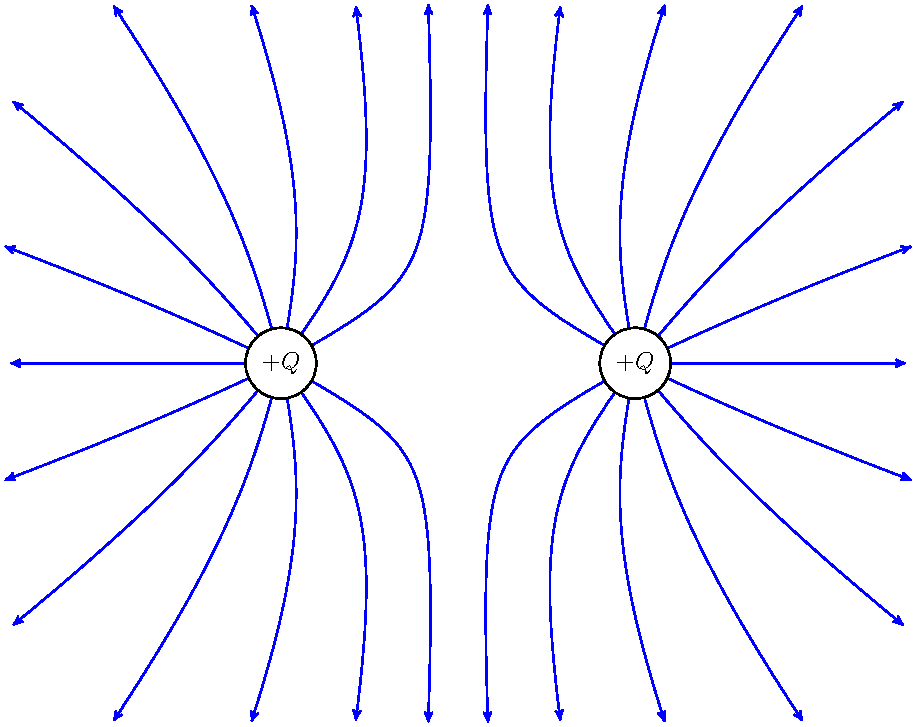
\includegraphics[width=7.2cm]{f-lines-eq-ch.pdf}
			\begin{equation*}
			\text{two positive charges}
			\end{equation*}
		\end{center}
	\end{minipage}\hfill
	\begin{minipage}{0.48\textwidth}
		\begin{center}
			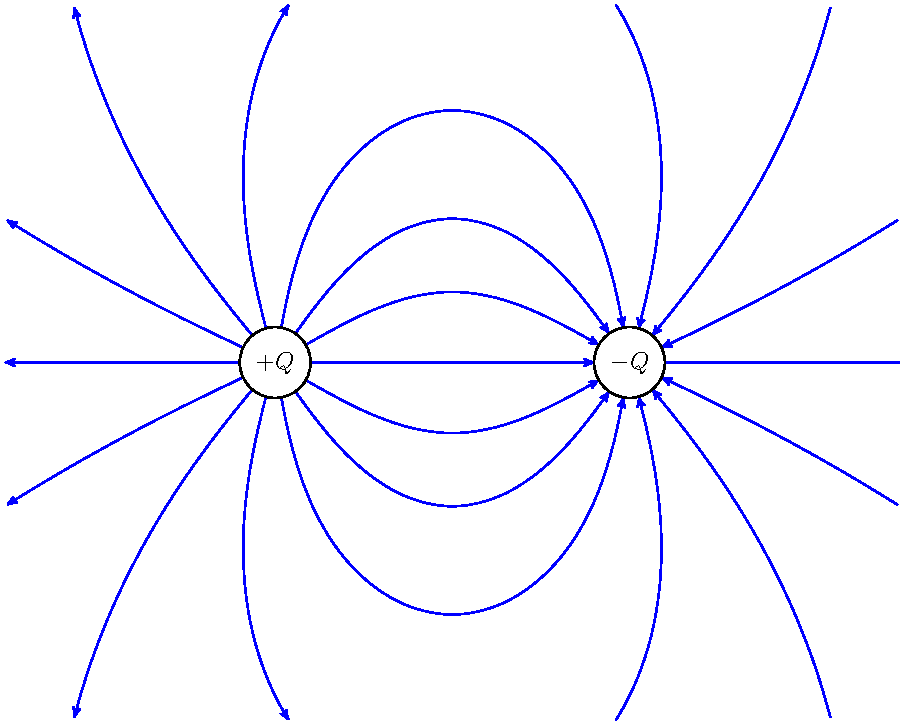
\includegraphics[width=7.2cm]{f-lines-op-ch.pdf}
			\begin{equation*}
			\text{two opposite charges} 
			\end{equation*}
		\end{center}	
	\end{minipage}
\end{figure*}

\section{potential \& potential energy }

\subsection{electric potential energy}
\label{sec:electric-potential}

gain/loss in \keypoint{electric potential energy}\index{electric field!electric potential energy} is defined as work done against/by electric force

(compare everything in this chapter with what you have learned about gravitational P.E.!)

let's start to derive the electrical P.E. between two charges $Q$ and $q$ separated by $r$

again we define $E_p=0$ at $r=\infty$ (choice of zero potential energy, no force so no P.E.), then

\begin{ilight}
	\keypoint{electric potential energy} is equal to the work done by electric force to bring a charge to a specific position from \emph{infinity}
\end{ilight} 

moving a test charge $q$ from $r=\infty$ to a distance of $r$ from $Q$

\begin{center}
\begin{tikzpicture}[scale=0.8]
\draw [fill] (-4,0) circle [radius=0.1];
\node[below] at (-4,-0.1) {$Q$};
\draw [fill] (8,0) circle [radius=0.1];
\node[below] at (8,-0.1) {$q$};
\draw [thick, <->] (0,-1.2) --(-4,-1.2) node[above,midway]{$r$};
\draw [thick,dashed,gray,->] (7.7,0) -- (0.3,0) node[above,midway]{\textcolor{black}{$W$}};
\draw [fill] (0,0) circle [radius=0.1];
\draw (8,-1) node{$\infty$};
\end{tikzpicture}
\end{center}

work done by electric force: $W=\int^r_\infty F dr = \int^r_\infty \frac{Qq}{\ec} \frac{\dd x}{x^2} = - \frac{Qq}{\ec x}\bigg|^r_\infty = - \frac{Qq}{\ec r} $

\eqyskip

since $\Delta E_p=-W$, we find: $E_p(r) - E_p(_\infty) = \frac{Qq}{\ec r}$

but $E_p(_\infty) = 0$,  so electric P.E. between two charges $Q$ and $q$ is $\tcbhighmath{E_p(r) = \frac{Qq}{\ec r}}$

\cmt as $r \to \infty$, $E_p \to 0$, this agrees with our definition for zero P.E. point

\cmt for like charges, $Qq > 0$, so $E_p > 0$

to bring like charges closer, work must be done to overcome their \emph{repulsion}, P.E. increases

minimum P.E. $E_p(\infty)=0$ at infinity, so positive P.E. at finite $r$

\cmt for opposite charges, $Qq < 0$, so $E_p < 0$

to pull opposite charges apart, work must be done to overcome their \emph{attraction}, P.E. increases

maximum P.E. $E_p(\infty)=0$ at infinity, so negative P.E. at finite $r$

\cmt electric P.E. is a \emph{scalar quantity}, sign is important

repulsion implies positive P.E., and attraction implies negative P.E.

sign of P.E. is hidden in polarities of charges


\example{To gain information about the gold nucleus ($_{\phantom{0}79}^{197}\text{Au}$), we fire $\alpha$-particles ($_2^4\alpha$) towards a thin gold foil. The size of a typical nucleus is about $10^{-14}$m, what is the minimum initial speed for $\alpha$-particles so that radius of gold nucleus can be determined?}
	
\begin{soln} as $\alpha$-particle approaches the nucleus, it slows down due to the repulsive interaction

kinetic energy decreases and electric potential energy increases

if it gets close enough to the nucleus before coming to a stop, nuclear radius can be estimated

{

\centering

$\text{K.E. loss} = \text{P.E. gain} \RA \frac{1}{2}mu^2 - \underbrace{\frac{1}{2}mv^2}_0 = E_p(r) - \underbrace{E_p(\infty)}_0 \RA  \frac{1}{2}mu^2= \frac{Qq}{4\pi\epsilon_0r}$

}

\begin{equation*}
	\frac{1}{2}\times4\times1.66\times10^{-27}\times u^2 = \frac{79\times1.60\times10^{-19}\times2\times1.60\times10^{-19}}{4\pi\times8.85\times10^{-12}\times10^{-14}} \end{equation*}
 \begin{equation*} 
 \RA	u\approx 3.3\times10^7\mps 
\end{equation*}
\end{soln}

\question{A metal sphere of radius 20 cm carries a charge of $5.0\times10^{-7}$ C. A proton is sent towards the sphere at a speed of $1.8\times10^6 \mps$. Can the proton reach the surface of the sphere?}



\subsection{electric potential}

it is also useful to define the \emph{electric potential} for any specific point in a field

electric potential can be thought as the electric potential energy per unit charge: $V = \frac{E_p}{q}$

\begin{ilight}
	\keypoint{electric potential}\index{electric field!electric potential} is the work needed to bring a unit positive charge from infinity
\end{ilight}

\cmt unit: $[V] = \text{ J C}^{-1} = \text{V}$

\cmt electric potential due to an isolated source $Q$: $V = \frac{E_p}{q} = \frac{\frac{Qq}{\ec r}}{q} \RA \tcbhighmath{V = \frac{Q}{4\pi\epsilon_0 r}}$

\cmt potential at infinity vanishes: $V_\infty = 0$

\cmt electric potential can take both signs

the sign depends on whether unit positive charge is repelled or attracted by the source

for positively-charged sources $V>0$, while for negatively-charged sources $V<0$

\cmt electric potential is a \emph{scalar} quantity

to find combined potential due to multiple charges, add up contributions of each charge

\example{An electron is accelerated from rest through a potential difference of 600 V.
	
Find the final speed of the electron.}

\begin{soln} gain in K.E. = change in electric P.E. $\RA \frac{1}{2}mv^2 = q\Delta V$
\eqyskip\begin{equation*}
	v = \sqrt{\frac{2q\Delta V}{m}} = \sqrt{\frac{2\time 1.60\times10^{-19}\times600}{9.11\times10^{-31}}} \approx 1.45\times10^7 \mps 
\end{equation*}
\end{soln}

\example{Two small metal spheres $A$ and $B$ are in a vacuum. Sphere $A$ has charge $+20$ pC and sphere $B$ has charge $+84$ pC. The arrangement is shown below.}

\begin{figure}[ht]
	\centering
	\begin{tikzpicture}
		\draw[thick] (-5,0) circle(0.8) node[above]{$A$} (5,0) circle(0.8) node[above]{$B$};
		\draw[thick,dashed] (-5,-2.1) -- (-5,0) -- (5,0) -- (5,-2.1) (-2,0) node[above]{$P$} -- (-2,-1.5)
		(0,0) node[above]{$M$} -- (0,-1.5);
		\draw[fill] (-2,0) circle(0.05);
		\draw[fill] (0,0) circle(0.05);
		\draw[<->] (-5,-2.0) -- (5,-2.0) node[midway,above]{$10$ cm};
		\draw[<->] (-5,-1.2) -- (-2,-1.2) node[midway,above]{$3.0$ cm};
		\draw[<->] (0,-1.2) -- (-2,-1.2) node[midway,above]{$2.0$ cm};
	\end{tikzpicture}
\end{figure}

(a) Find the electric potential at point $P$ and point $M$ respectively.

(b) Find the work done to move an $\alpha$-particle from $P$ to $M$.

\begin{soln} combined electric potential: $V = V_A + V_B = \frac{1}{\ec}\left(\frac{Q_A}{r_A} + \frac{Q_B}{r_B} \right)$


at $P$: $V_P = 8.99\times10^9 \times \left( \frac{+20 \times 10^{-12}}{0.030} + \frac{+84 \times 10^{-12}}{0.070} \right) \approx 16.8 \text{ V}$

\eqyskip

at $M$: $V_M = 8.99\times10^9 \times \left( \frac{+20 \times 10^{-12}}{0.050} + \frac{+84 \times 10^{-12}}{0.050} \right) \approx 18.7 \text{ V}$

from $P$ to $M$: $W = \Delta E_p = q\Delta V = q(V_M- V_P) = 2\times1.60\times10^{-19}\times(18.7-16.8) \approx 6.2\times10^{-19} \text{ J}$ \end{soln}

\example{$A$ and $B$ are two positively-charged spheres of radius 1.0 cm. A proton $P$ initially at rest on the surface of $A$ moves along the line joining the centres of the two spheres. The variation with distance $x$ from the centre of $A$ of electric potential $V$ at point $P$ is given.}\label{ex-V-of-two-pcs}

\begin{figure}[ht]
	\centering
	\begin{tikzpicture}[scale=1.2]
		\draw[style=help lines,step=0.2,gray!50] (0,-0) grid (6,5);
		\draw[step=1] (0,0) grid (6,5);
		\draw [very thick, color=blue, domain=0.5:5.5, smooth, samples=60, variable=\x] plot (\x,{2.2/\x + 1.1/(6-\x)});
		\draw[very thick,blue] (0,4.6) --++ (0.5,0) node[above]{$A$};
		\draw[very thick,blue] (5.5,2.6) node[above]{$B$} --++ (0.5,0);
		\foreach \x in {0,100,200,300,400,500} \node[left] at (0,\x/100) {$\x$};
		\foreach \x in {0,2,4,6,8,10,12} \node[below] at (\x/2,0) {$\x$};
		\node at (-1.35,2.5) {$V/\text{V}$};
		\node at (3,-0.8) {$x/\text{cm}$};
	\end{tikzpicture}
\end{figure}

\rcyskip (a) Find the maximum speed as the proton moves from $A$ to $B$.

(b) Find the speed when the proton reaches surface of $B$.

\begin{soln}
    
increase in K.E. = loss in P.E., so: $\frac{1}{2}mv^2 - 0 = q\Delta V \RA \frac{1}{2}mv^2 = q(V_A - V_P)$

maximum speed when $\Delta V$ is maximum, or $V_P = 107 \text{ V}$ becomes minimum (at $x = 7.2$ cm)
\begin{equation*}
	\frac{1}{2}\times1.67\times10^{-27}\times v^2_\tmax = 1.60\times10^{-19} \times (460-107) 
 \end{equation*}
 \begin{equation*}
 \RA v_\tmax \approx 2.60\times10^5 \mps
\end{equation*}

at surface of $B$, $V_P = 260 \text{ V}$ (at $x=11.0$ cm)
\begin{equation*}
\frac{1}{2}\times1.67\times10^{-27}\times v^2_B = 1.60\times10^{-19} \times (460-260) 
 \end{equation*}
 \begin{equation*}
\RA v_B \approx 1.96\times10^5 \mps 
\end{equation*}
\end{soln}

\question{Electrical breakdown occurs when electric field strength at surface of a metal sphere exceeds $5.0 \times 10^6 \NpC$. Given that the radius of the sphere is 16 cm. What is the electric potential at the surface when electrical breakdown occurs?}

\question{Two charged particles $A$ and $B$ are separated by 20 cm. $P$ is a point on the line $AB$. Given that particle $A$ carries charge $+7.2 \text{ }\mu\text{C}$, and electric potential is zero where $AP = 5.0$ cm. Find the electric charge of $B$.}

\question{A particle with specific charge (ratio of its electric charge to its mass) $+9.58\times10^7 \text{ C kg}^{-1}$ is moving towards a fixed metal sphere. The sphere has a potential of $+500$ V. The initial speed of the particle is $3.0\times10^5 \mps$ when it is a large distance from the sphere. Determine whether the particle can reach the surface of the sphere.}


\subsection{equipotential lines}

to show potential distributions, we draw \keypoint{equipotential lines}\index{equipotential lines}
\footnote{In three dimensions, these lines form equipotential \emph{surfaces}.}

points on same equipotential line have constant electric potential

i.e., equipotential lines are \emph{contour lines} of equal electric potential

\cmt for a field near a point charge, equipotential lines are a set of \emph{concentric} circles

\begin{center}
	\begin{tikzpicture}[scale=1.35]
	\draw (-2.7,0) node{$+Q$} circle [radius=0.5];
	\foreach \s in {0,45,90,...,315}
	\draw [blue, thick, ->] (-2.7,0) ++ (\s:0.5) -- ++(\s:1.8);
	
	\draw (2.7,0) node{$-Q$} circle [radius=0.5];
	\foreach \s in {0,45,90,...,315}
	\draw [blue, thick, <-] (2.7,0) ++ (\s:0.5) -- ++(\s:1.8);
	
	\foreach \s in {0.9,1.4,1.9}{
		\draw [red,dashed] (-2.7,0) circle(\s) (2.7,0) circle(\s);}
	\end{tikzpicture}
\end{center}

\cmt for uniform fields, equipotential lines are a set of \emph{parallel} straight lines

\begin{center}
	\begin{tikzpicture}[yscale=1.2]
	\draw (-5,1.2) rectangle (5,1.6);
	\draw (-5,-1.2) rectangle (5,-1.6);
	\foreach \charge in {-4.5,-3.5,...,4.5}{
		\draw (\charge,1.4) node {$+$} (\charge,-1.4) node {$-$};
		\draw[thick,blue,->] (\charge,1.2) --++ (0,-2.4);	
	}
	\foreach \s in {-0.8,0,0.8} \draw[red,dashed] (-5,\s) -- (5,\s);
	\end{tikzpicture}
\end{center}
	

	
\cmt equipotential lines are always perpendicular to the electric field lines
	
moving along an equipotential line requires no work done

\example{Field lines and equipotential lines due to two charges of various magnitudes}

\begin{figure*}
	\noindent\begin{minipage}{0.48\textwidth}
		\begin{center}
			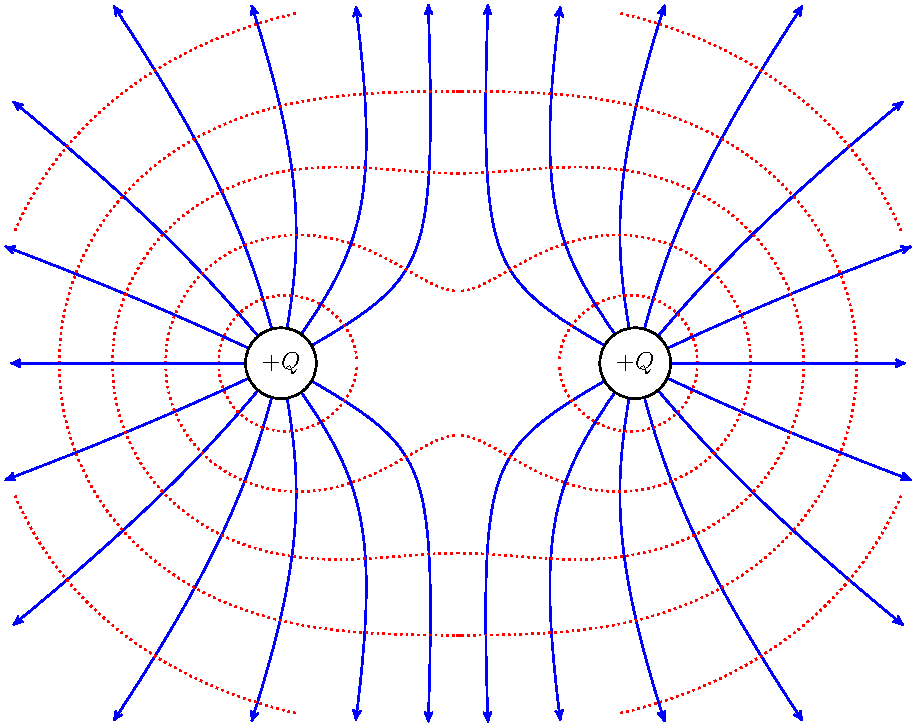
\includegraphics[width=7cm]{f-all-eq-ch.pdf}
		\end{center}
	\end{minipage}\hfill
	\begin{minipage}{0.48\textwidth}
		\begin{center}
			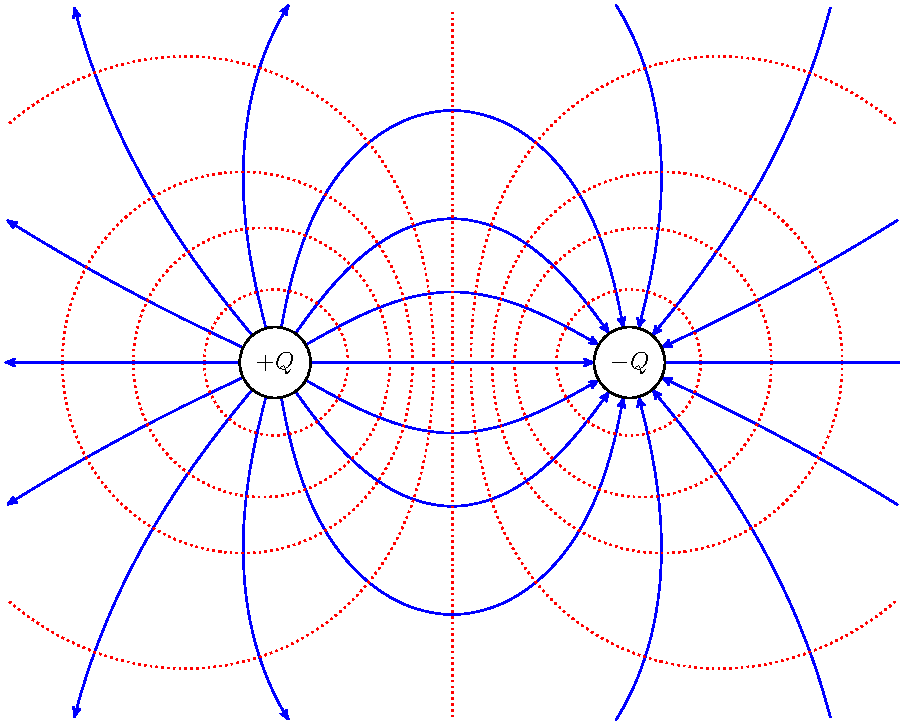
\includegraphics[width=7cm]{f-all-op-ch.pdf}
		\end{center}
	\end{minipage}
\end{figure*}

\begin{figure*}	
	\noindent\begin{minipage}{0.48\textwidth}
		\begin{center}	
			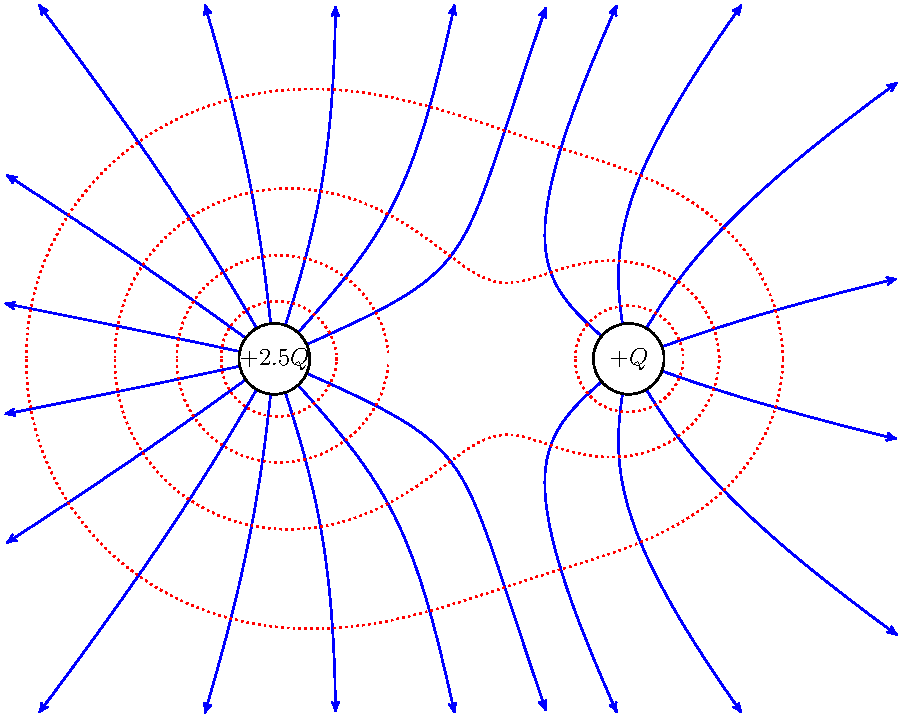
\includegraphics[width=7cm]{Q2p.pdf}
			\end{center}
		\end{minipage}\hfill
	\begin{minipage}{0.48\textwidth}
		\begin{center}
			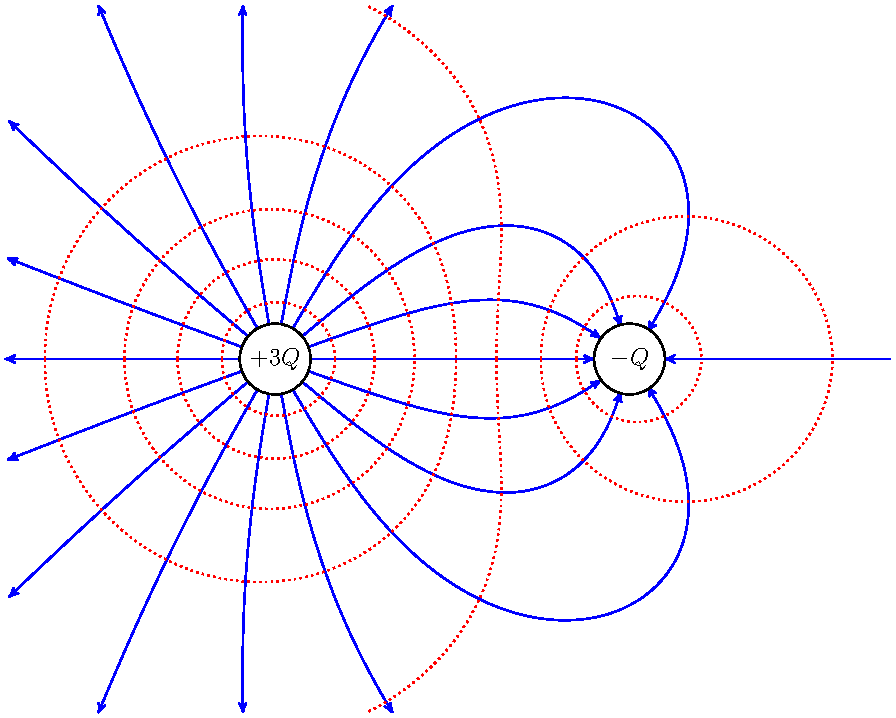
\includegraphics[width=7cm]{Q4n.pdf}
		\end{center}
	\end{minipage}
\end{figure*}

\begin{figure*}	
	\noindent\begin{minipage}{0.48\textwidth}	
		\begin{center}	
			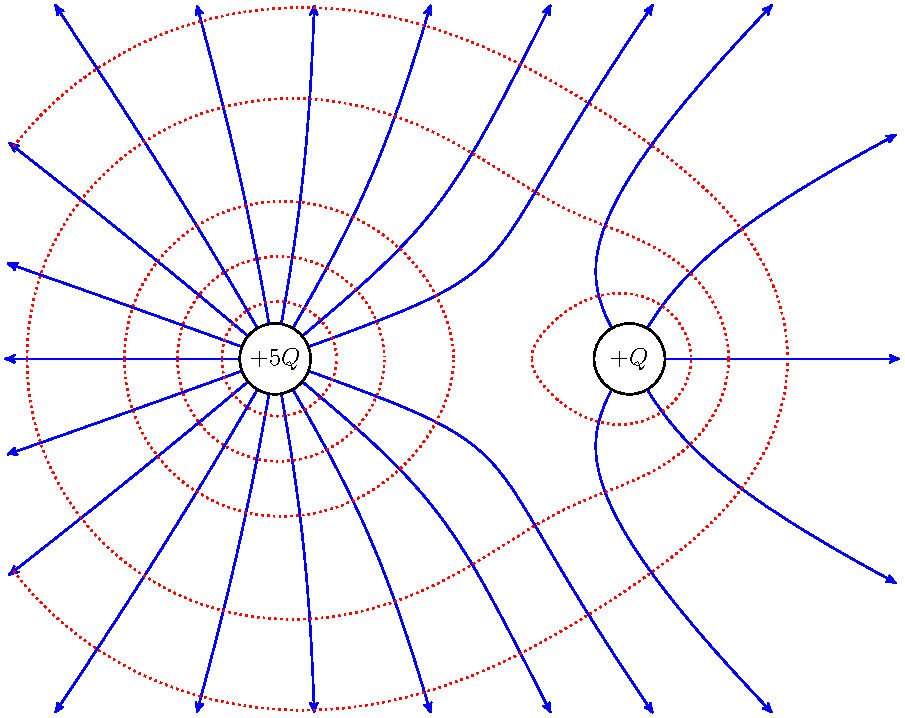
\includegraphics[width=7cm]{Q5p.pdf}
		\end{center}
	\end{minipage}\hfill
	\begin{minipage}{0.48\textwidth}
		\begin{center}
			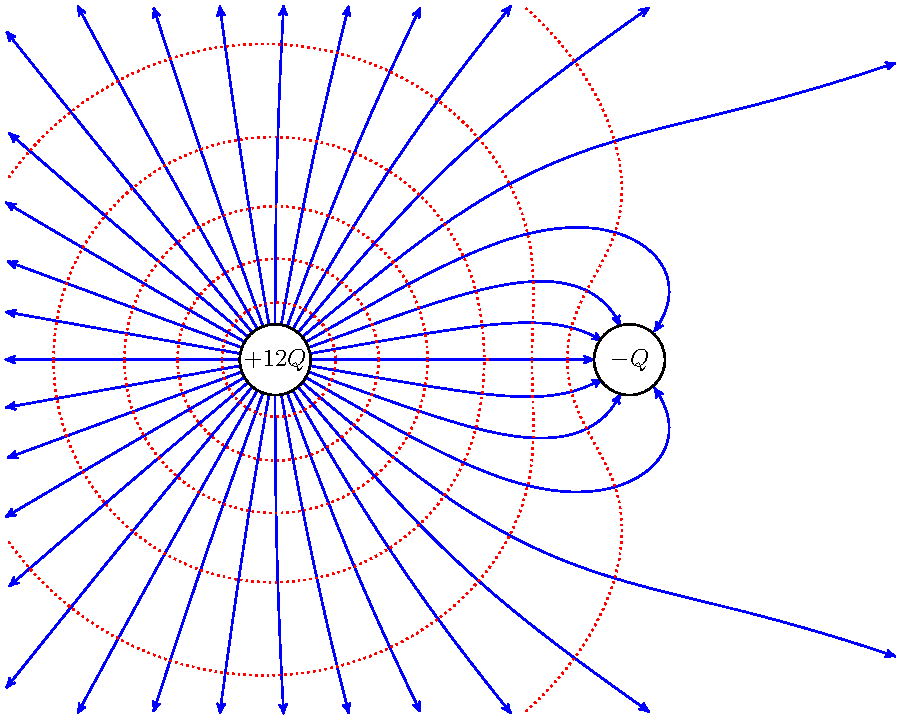
\includegraphics[width=7cm]{Q12n.pdf}
		\end{center}	
	\end{minipage}
\end{figure*}



\subsection{further discussions on electric fields}

\subsection{comparison with gravitational fields}

both gravitational and electric force are described by inverse square law, so it follows that the mathematical language for both theories are very similar

\cmt physical quantities that describe gravitational/electric fields
\cmt comparing gravitational field with electric field
\footnote{Note that there is no negative mass, gravitational force always interacts attractively. This is the fundamental difference between gravitational fields and electric fields.}

\begin{center}
	\begin{tabular}{|c|c|c|}
		\hline
		& vector description & scalar description \\ \hline 
		interaction between two masses/charges & force $F$ & potential energy $E_p$ \\ \hline
		effect of source mass/charge & field $g$/$E$ & potential $\varphi$/$V$ \\ \hline
	\end{tabular}
\end{center}

\begin{center}
{\renewcommand{\arraystretch}{1.28}
\begin{tabular}{|c|c|c|c|}
\hline
& gravitational field & electric field & meaning \\ \hline 
force & $F=(-)G \frac{Mm}{r^2}$ & $F=\frac{1}{4\pi\epsilon_0} \frac{Qq}{r^2}$ & force between masses/charges\\ [1ex] \hline
field strength & $g= \frac{F}{m} = (-)G \frac{M}{r^2}$ & $E= \frac{F}{q} = \frac{1}{4\pi\epsilon_0} \frac{Q}{r^2}$ & force per unit mass/charge\\ [1ex] \hline
potential energy &  $E_p = -G \frac{Mm}{r}$ & $E_p=\frac{1}{4\pi\epsilon_0} \frac{Qq}{r}$ & related to work done by force \\ [1ex] \hline
potential & $\varphi = \frac{E_p}{m} = -G \frac{M}{r}$ & $V = \frac{E_p}{q} = \frac{1}{4\pi\epsilon_0} \frac{Q}{r}$ & energy per unit mass/charge\\ [1ex] \hline
\end{tabular}}
\end{center}

\cmt similarities between gravitational field and electric field

\begin{itemize}
	\item[-] force and field strength both obey \emph{inverse square laws}
	
	\item[-] potential energy and potential is inversely proportional to separation
	
	\item[-] no potential energy and no potential at infinite separation
\end{itemize}

\cmt differences between gravitational field and electric field

mass (source of gravity) is always positive, but electric charges can be positive or negative

this fact leads to many fundamental differences between the two force fields

\begin{itemize}
\item[-] electric force can be repulsive or attractive, but gravitational force is always attractive

\item[-] electric potential can take both signs, but gravitational potential is always negative
\end{itemize}

\subsection{electric field inside conductors}\label{inside-conductors}

consider electric field \emph{inside} a metal conductor carrying charge $Q$

conductor means there are free charge carriers that can move around 

but charge distribution should be stable for a charged conductor (no circulating currents)

so charge carriers must experience no force, i.e., field strength inside conductor is zero

put it the other way round, if there is an excess field, it will push free charge carriers to move around, until they are distributed so that the field inside the conductor becomes zero

moreover, there shall be no potential difference between any two points inside the conductor, otherwise charge carriers would flow, so electric potential must be constant

\begin{ilight}
	\centering
	
	electric field strength is everywhere zero inside a conductor: $E=0$
	
	electric potential is everywhere constant inside a conductor: $V=\text{const}$
\end{ilight}

\example{Consider the electric field due to a metal sphere of radius $R$ carrying charge $Q$. Plot the variation with the distance $r$ from sphere's centre of the field strength, and the variation with $r$ of the electric potential.}\label{ex-metal-sphere}


\begin{soln}
charge $Q$ is uniformly spread out on \emph{surface} of sphere

viewed from \emph{outside}, the sphere appears to have all of its charge concentrated at the centre

so it can be modelled as a point charge due to its symmetric distribution of charges

electric field strength at distance $r$ from sphere's centre is: $E = \frac{Q}{\ec r^2}$ for $r>R$

electric potential at distance $r$ from sphere's centre is: $V=\frac{Q}{4\pi\epsilon_0r}$ for $r>R$

\emph{inside} the sphere, i.e., for $r<R$, we have $E=0$, and $V=\frac{Q}{\ec R} = \text{const}$ \end{soln}

\begin{figure*}[ht]
	\centering
	\noindent\begin{minipage}{0.45\linewidth}
		\centering
		\begin{tikzpicture}[yscale=1.2,xscale=1.2]
		\draw[thick,<->] (0,5) node[left]{$E$} -- (0,0) -- (1,0) node[below]{$R$} -- (4.5,0) node[below]{$r$};
		\draw [thick,color=blue,domain=1:4.5,samples=20,smooth,variable=\x] plot (\x,{4.5/\x/\x});
		\draw[thick,blue] (0,0.02) -- (1,0.02);
		\draw[dashed] (0,4.5) node[left]{$E_0$} -- (1,4.5) -- (1,0) node[below]{$R$};
		\draw[dashed] (0,4.5/4) node[left]{{\scriptsize $\frac{E_0}{4}$}} -- (2,4.5/4) -- (2,0) node[below]{$2R$};
		\draw[dashed] (0,4.5/9) node[left]{{\scriptsize $\frac{E_0}{9}$}} -- (3,4.5/9) -- (3,0) node[below]{$3R$};
		\end{tikzpicture}
		

	\end{minipage}
	\begin{minipage}{0.45\linewidth}
		\centering
		\begin{tikzpicture}[yscale=1.2,xscale=1.2]
		\draw[thick,<->] (0,5) node[left]{$V$} -- (0,0) -- (1,0) node[below]{$R$} -- (4.5,0) node[below]{$r$};
		\draw [thick,color=blue,domain=1:4.5,samples=20,smooth,variable=\x] plot (\x,{4.5/\x});
		\draw[dashed] (0,4.5) node[left]{$V_0$} -- (1,4.5) -- (1,0) node[below]{$R$};
		\draw[dashed] (0,4.5/2) node[left]{{\scriptsize $\frac{V_0}{2}$}} -- (2,4.5/2) -- (2,0) node[below]{$2R$};
		\draw[dashed] (0,4.5/3) node[left]{{\scriptsize $\frac{V_0}{3}$}} -- (3,4.5/3) -- (3,0) node[below]{$3R$};
		\draw[thick,blue] (0,4.5) -- (1,4.5);
		\end{tikzpicture}
		

	\end{minipage}

\caption{Example \ref{ex-metal-sphere}: field strength and potential due to a charged metal sphere}
\end{figure*}


\question{State whether the two spheres in Example \ref{ex-V-of-two-pcs} are conductors. State what feature of the potential graph supports your answer.}

\question{You might have the experience that your mobile phone signal gets much weaker when you get into an elevator. Explain why this happens.}

\subsection{field strength \& potential}\label{field-strength-potential}

for a small displacement $\Delta r$ in an electric field, change in potential $\Delta V$ is

{

\centering

$\Delta V = \frac{\Delta E_p}{q} \xlongequal{\Delta E_p=-W} - \frac{\Delta W}{q} = - \frac{F \Delta r}{q} \xlongequal{F=Eq} - E \Delta r \RA E = - \frac{\Delta V}{\Delta r}$

}

\eqyskip as change in displacement $\Delta r \to 0$, we have $\tcbhighmath{E = - \frac{\dd V}{\dd r}}$

therefore we have the following theorem:

\begin{ilight}
	\centering field strength is negative gradient of potential with respect to displacement
\end{ilight}

\newpage

can also consider change in potential $\Delta V$ for large distance due to work done in a field

{
	
\centering

$\Delta V= \int \dd V \xlongequal{E = -\dd V/\dd r}  \int (-)E \dd r =  -\int E \dd r$
\footnote{The expression is implicitly integrated from initial position to final position.}

}

\eqyskip this gives the inverse relation: $\tcbhighmath{\Delta V = -\int E \dd r}$
\footnote{These equations are correct if the charge is moving in the parallel direction to the field, i.e., the motion is along the field lines. But an object can move in all directions in the field. More rigorously, if we take the vector nature of electric field into account, we should write $\Delta V = - \int \mathbf{E}\cdot\dd\mathbf{r}$, and $\mathbf{E} = - \frac{\partial V}{\partial \mathbf{r}}$. \piste}

\cmt given a $V$-$r$ graph, gradient of curve gives field strength

conversely, given a $E$-$r$ graph, area under curve gives change in potential

\cmt can also write $F = - \frac{\dd U}{\dd r}$ and $\Delta U = -\int F \dd r$

force always acts in a direction to lower the potential energy of an object
\footnote{This result can be generalised to a very important principle of physical laws called the \emph{least action principle}. It states that any motion of a system tends to minimise the action, a physical quantity related to the energy of the system. This fundamental law plays a crucial role in the study of theoretical physics. \piste}

\example{The variation of electric potential near a charged object is shown on the graph. Calculate the electric field strength at 5.0 cm from the centre of the object.}\label{ex-grad-pot}

\begin{figure}[ht]
	\centering
	\begin{tikzpicture}[scale=0.54]
	\draw[style=help lines,step=0.5,gray!30] (0,0) grid (12,12);
	\draw[style=help lines,step=2] (0,0) grid (12,12);
	\draw [thick] (12,0) node[below]{$r/\text{cm}$};
	\draw [thick] (0,12) node[left]{$V/\text{kV}$};
	\foreach \s in {0,2,...,10}
	{
		\draw (\s,0) node[below]{\s};
		\draw (0,\s) node[left]{\s};
	}
	\draw[very thick,purple,domain=2:10,samples=15,smooth,variable=\x] plot (\x,20/\x);
	\draw[thick,red,domain=1:9,samples=2,smooth,variable=\x] plot (\x,-0.8*\x+8);
	\draw[fill] (5,4) circle[radius=0.15];
	\draw[thick,blue] (2,6.5) -- (2,1.5) -- (8,1.5);
	\end{tikzpicture}
\end{figure}

\begin{soln} draw tangent to the graph at $r=5.0\text{ cm}$ (red line), gradient of tangent gives field strength:

$ \text{gradient} = \frac{\Delta V}{\Delta r} = \frac{(1.5-6.5)\times 10^3}{(8.0-2.0)\times10^{-2}} \approx  -8.3\times10^4 \Vpm \RA E = -\frac{\Delta V}{\Delta r} = 8.3\times10^4 \Vpm $ \end{soln} 

\newpage

\question{Show that the charged object in Example \ref{ex-grad-pot} behaves like a point charge. Determine the charge it carries, and hence calculate the field strength at $r=5.0$ cm.}

\example{The variation of electrical potential along a certain line is shown. State and explain where in the field an electron will experience the greatest force.}

\begin{figure}[ht]
	\centering
	\begin{tikzpicture}[scale=1.35]
	\draw[style=help lines,step=0.25,gray!30] (0,-2) grid (8,4);
	\draw[style=help lines,step=1] (0,-2) grid (8,4);
	\node[left] at (0,4) {$V$};
	\node[left] at (0,0) {0};
	\foreach \x in {0,1,...,8} {
		\draw[white,fill] (\x-0.1,-0.32) rectangle (\x+0.1,-0.08);
		\node[below] at (\x,0) {$\x$};
	}
	\draw[thick, purple, domain=1:7, samples=25, smooth, variable=\x] plot (\x,{4/\x/\x-2/(8-\x)/(8-\x)});
	\node[right] at (8.1,0) {$x/\text{cm}$};
	\end{tikzpicture}
\end{figure}

\begin{soln} greatest force means greatest field strength, which means maximum potential gradient 

largest gradient of $V$-$x$ curve at $x=1$ cm, so greatest force at $x=1$ cm \end{soln}

\example{electric field due to an isolated point charge}

we have learned that the electric potential due to a point charge is: $V = \frac{Q}{\ec r}$
	
using $E = -\frac{\dd V}{\dd r}$, we have $E = -\frac{\dd}{\dd r}\left( \frac{Q}{4\pi\epsilon_0r} \right) = -\frac{Q}{4\pi\epsilon_0}\frac{\dd}{\dd r}\left(\frac{1}{r}\right) = \frac{Q}{4\pi\epsilon_0r^2}$

this agrees with the expression for field strength due to an isolated charge \eoe

\question{For the electric field due to a charged metal sphere (see Example \ref{ex-metal-sphere}), convince yourself that the field strength equals negative gradient of potential at any point.}

\question{We have seen the statement field strength equals negative potential gradient holds for electric fields. Does it also hold for gravitational fields?}




\subsection*{uniform fields revisited}

given two oppositely-charged metal plates separated by a distance of $d$

if p.d. between the plates is $V$, then electric field strength between is given by $E = \frac{V}{d}$\footnote{You should have learned this in AS-level physics.}

we will derive this result using the theorem introduced in the last chapter

\begin{figure}[ht]
\centering
\begin{minipage}{0.48\textwidth}
	\centering
	\begin{tikzpicture}[scale=0.8]
	\foreach \s in {1,2,3,4}
	\draw[thick,blue,<-] (0,\s) -- (5,\s);
	\draw (2.5,4) node[above]{$E$};
	\draw [thick,gray,dashed,<-] (1,2.5) -- (4,2.5);
	\shade [ball color = green] (4,2.5) circle [radius=0.1] node[right]{$q$};
	\draw [thick] (5,0.5) -- (5,4.5) node[above]{$+$};
	\draw [thick] (0,0.5) -- (0,4.5) node[above]{$-$};
	\draw[<->] (0,0) -- (5,0) node[midway, above] {$d$};
	\end{tikzpicture}
\end{minipage}\hfil
\begin{minipage}{0.48\textwidth}
	\centering
	\begin{tikzpicture}[scale=0.8]
		\draw [thick,<->] (0,4.2) node[left]{$V$} -- (0,0) -- (5.6,0) node[below]{$r$};
		\draw[dashed] (5,3.6) -- (5,0) node[below]{$d$}; 
		\draw [very thick,red] (0,0) -- (5,3.6);
	\end{tikzpicture}
\end{minipage}
\captionsetup{labelformat=empty}

\caption{moving a test charge in a uniform electric field}
\end{figure}


moving a test charge $q$ in a uniform field, work done by electric force: $W=Fd = Eqd$
		
change in P.E.: $\Delta E_p = -W = -Eqd$

change in potential: $\Delta V = \frac{\Delta E_p}{q} = - Ed$, or $E=-\frac{\Delta V}{d}$

plotting $V$-$r$ graph, $\text{gradient of line}=-E$

the minus sign means field strength points in the direction such that potential decreases

i.e., electric field acts from high potential to low potential



\subsection*{electric field due to two positive point charges}

two point charges $+Q_1$, $+Q_2$ are separated by a distance of $D$

let's look into the electric field along the segment joining the two charges 

\begin{center}
\begin{tikzpicture}[scale=0.8]
\shade [ball color = green] (-4,0) node[above]{$+Q_1$} circle (0.15);
\shade [ball color = green] (4,0) node[above]{$+Q_2$} circle (0.15);
\draw [thick, <->] (-4,-2)--(4,-2) node[midway,above]{$D$} ;
\draw [thick, <->] (-4,-1)--(-1,-1) node[midway,above]{$r_1=x$};
\draw [thick, <->] (-1,-1)--(4,-1) node[midway,above]{$r_2=D-x$};
\draw [thick, <->] (-4,-2)--(4,-2) node[midway,above]{$D$} ;
\draw [dashed] (-4,-0.5) -- (-4,-2.2);
\draw [dashed] (4,-0.5) -- (4,-2.2);
\draw [dashed] (-1,-0.5) -- (-1,-1.5);
\draw [->,thick,blue] (-1,0) -- ++(-0.9,0) node[above]{$E_2$};
\draw [->,thick,blue] (-1,0) -- ++(2.5,0) node[above]{$E_1$};
\draw [fill] (-1,0) node[above]{$q$} circle [radius=0.1];
\end{tikzpicture}
\end{center}

combined potential: $V = V_1 + V_2 = \frac{Q_1}{4\pi\epsilon_0r_1} + \frac{Q_2}{4\pi\epsilon_0r_2} = \frac{1}{4\pi\epsilon_0}\left(\frac{Q_1}{x} + \frac{Q_2}{D-x}\right)$

combined field strength: $E = E_1 - E_2 = \frac{Q_1}{4\pi\epsilon_0r_1^2} - \frac{Q_2}{4\pi\epsilon_0r_2^2} = \frac{1}{4\pi\epsilon_0}\left(\frac{Q_1}{x^2} - \frac{Q_2}{(D-x)^2}\right)$

notice that when computing $V$, we carry out \emph{scalar sum}

but for $E$, we carry out \emph{vector sum}, i.e., directions of $E_1$ and $E_2$ become important

$V$-$x$ graph and $E$-$x$ graph for the case where $Q_1=3Q_2$ are sketched

\begin{center}
	\begin{tikzpicture}[scale=1.35]
	\draw[thick,->] (0,-2) -- (0,4.8);
	\draw[thick,->] (0,0) -- (9,0) node[below]{$x$};
	\draw [thick,color=blue,domain=0.3:7.7,samples=60,smooth,variable=\x] plot (\x,{(.24/\x/\x-.08/(8-\x)/(8-\x))*1.5}) node[below]{$E$};
	\draw [thick,color=red,domain=0.3:7.7,samples=60,smooth,variable=\x] plot (\x,{(.3*3/\x+.1*3/(8-\x))*1.5}) node[above]{$V$};
	\draw[dashed] (8,-2) -- (8,3);
	\shade [ball color = green] (0,0) node[below right]{$+Q_1$} circle (0.15);
	\shade [ball color = green] (8,0) node[below right]{$+Q_2$} circle (0.15);
	\end{tikzpicture}
\end{center}

\question{Convince yourself that field strength is indeed given by negative potential gradient. You may interpret it either graphically (think about gradient of tangent along the curve) or algebraically (think about the derivative of $V$).}

\question{We have looked into the electric field between two positively-charged particles. Discuss the cases where (a) both particles are negatively charged, (b) the two particles carry opposite charges.}
% \chapter{Capacitors}

\section{Capacitors: an introduction}

\begin{marginfigure}
\begin{tikzpicture}[scale=0.5]
\coordinate (A1) at (0,0); 
\coordinate (A2) at (0.5,0);
\coordinate (A3) at (2.5,0); 
\coordinate (A4) at (3,0);
\coordinate (B1) at (0,4); 
\coordinate (B2) at (0.5,4);
\coordinate (B3) at (2.5,4); 
\coordinate (B4) at (3,4);
\coordinate (C1) at (1.2,5.5); 
\coordinate (C2) at (1.7,5.5);
\coordinate (C3) at (3.7,5.5); 
\coordinate (C4) at (4.2,5.5);
\coordinate (D4) at (4.2,1.5);
\draw [thick,fill=gray!50] (A1) -- (A2) -- (B2) -- (C2) -- (C1) -- (B1) -- cycle;
\draw [thick,fill=cyan!20] (A2) -- (A3) -- (B3) -- (C3) -- (C2) -- (B2) -- cycle;
\draw [thick,fill=gray!50] (A3) -- (A4) -- (B4) -- (C4) -- (C3) -- (B3) -- cycle;
\draw [thick,fill=gray!50] (A4) -- (B4) -- (C4) -- (D4) -- cycle;
\draw [thick] (B1) -- (B4);
\draw [ultra thick] (3.6,2.7) [out=0, in=180] to (6,2) node[below]{lead};
\draw [ultra thick] (0,2.7) [out=180, in=0] to (-1.5,2) node[below]{lead};
\draw [thick] (3.6,4) -- ++ (1.5,1) node[right,align=center,execute at begin node=\setlength{\baselineskip}{1.2em}]{metal\\plate};
\draw [thick] (1.5,0.5) -- ++ (1.2,-1) node[right]{dielectric};
\end{tikzpicture}
\end{marginfigure}

\keypoint{Capacitors}\index{capacitor} are elementary electrical units widely used in electrical and electronic engineering. a typical capacitor has two conductive plates and between the plates there is usually an insulating material called \emph{dielectric}.

circuit symbol for a capacitor is:
\begin{figure}
    \centering
\begin{tikzpicture}[scale=0.2]
\draw (0,0) -- (1.6,0) (2.4,0) -- (4,0);
\draw (1.6,-1) -- (1.6,1) (2.4,-1) -- (2.4,1);
\end{tikzpicture}
\end{figure}
\vspace*{\baselineskip}

\begin{marginfigure}
\begin{circuitikz}[european resistors]
	\draw (2,-2) -- (-2,-2)  to[battery,l^=$\mathcal{E}$] (-2,2) -- (-0.5,2);
	\draw (2,-2) -- (2,-2)  to[R,l_=$R$] (2,2) -- (0.5,2);
	\draw (0,-2) -- (0,-1) to[C,l_=$C$] (0,1) -- (0,1.2);
	\draw[fill=white] (0.5,2) circle(0.06) node[above]{$Y$};
	\draw[fill=white] (-0.5,2) circle(0.06) node[above]{$X$};
	\draw[very thick] (0,1.2) --++ (80:1);
	\draw[fill=white] (0,1.2) circle(0.06) node[right]{$S$};
\end{circuitikz}
\end{marginfigure}

If we construct an electric circuit as shown, when contact $S$ is moved to $X$, capacitor is connected to a voltage supply and becomes charged. Positive and negative charges are separated onto two plates, and they will stay where they are even if we disconnect the capacitor from the voltage supply.

If we then move $S$ to $Y$, the charged capacitor discharges and drives a current through resistor $R$, i.e., it can act as a temporary power source\footnote{Details on charging and discharging processes will be gone through in \S\ref{sec:charging-capacitors}.}

So capacitors can be used to store and release energy, or more correctly, charge.\footnote{Other important functions of capacitors in electronic circuits include smoothing output voltage of power supplies, blocking direct current while allowing alternating current to pass, etc.}

\subsection{Capacitance}

To describe ability of a capacitor to store charges, we define the notion of capacitance

\begin{ilight}
	\keypoint{The capacitance}\index{capacitance!mutual capacitance} of a parallel-plate capacitor is defined as the ratio of the charge stored on each plate to the potential difference across the two plates.
\end{ilight}

In a word equation: $\text{Capacitance } C = \frac{\text{charge on one plate }Q }{\text{p.d. } V \text{ across the plates}} \quad \Rightarrow \quad$ $$\tcbhighmath{C = \frac{Q}{V}}$$

The unit of capacitance: \keypoint{farad}\index{farad}
\footnote{The unit is named after Michael Faraday, a British physicist who developed the concept of capacitance. Faraday's other main discoveries include electromagnetic induction and electrolysis. He established the basis for the concept of the electromagnetic field in physics.}
: $[C] = \text{F}$

It's a derived unit: $1 \text{ F} = 1 \text{ C}\cdot\text{V}^{-1}$

The Farad is a stupidly large unit for most applications, more common subunits of capacitance in use are sub-multiples of farad:

{
	
\centering

$1 \muF = 10^{-6} \text{ F}, \quad 1 \text{ nF} = 10^{-9} \text{ F}, \quad 1 \pF = 10^{-12} \text{ F}$

}

One important point that is often missed - for a parallel-plate capacitor, charges on the two plates are equal but opposite so the net charge on the capacitor: $Q_\text{net} = (+Q)+(-Q)=0$. 

I want to really emphasise that:
\begin{ilight}
    The charge in the definition is charge on \emph{one} plate \textbf{not} the difference between the plates.
\end{ilight}

The capacitance of a capacitor depends on \emph{geometry} of the device and permittivity of the dielectric material. It does not depend on electric field or potential\footnote{Recall the resistance of an electrical component. Resistance is defined as the ratio of p.d. to current, but the value of resistance is essentially dependent on the length, cross-sectional area and material of the component, instead of the p.d. applied or the current flowing through it.}

for example, capacitance between two metal plates isfootnote{If there is \emph{dielectric} in between, the formula should be rewritten as $C = \frac{\epsilon A}{d}$, where $\epsilon$ is permittivity of dielectric. These formulae are not examinable by the syllabus.}: $$\tcbhighmath{C=\frac{\epsilon_0 A}{d}}$$\

Where:\\
$A$ is area of plate, \\
$d$ is distance between plates, \\
both are geometrical quantities



% \subsection{self-capacitance}

% there are two closely related notions of capacitance: \emph{mutual} capacitance and \emph{self} capacitance

% the definition for capacitance given in the previous chapter, is actually \emph{mutual} capacitance\footnote{In many cases, the term capactiance is a shorthand for mutual capacitance.}

% on the other hand, all bodies are able to store electrical charge

% any object that can be electrically charged exhibits capacitance

% we define \keypoint{self-capacitance}\index{capacitance!self-capacitance} of an object as the amount of charge that must be added to increase per unit electrical potential

% in a word equation, $ \text{self capacitance }C=\frac{\text{charge of object }Q}{\text{electric potential of object }V} \RA \tcbhighmath{C=\frac{Q}{V}}$\footnote{For either mutual capacitance or self capacitance, defining equation $C=\frac{Q}{V}$ takes the same form, but you should keep in mind that $Q$ and $V$ represent different things in different contexts.}

% \example{Self-capacitance of a charged metal sphere in a vacuum}

% consider a metal sphere of radius $R$ and carries an electric charge of $Q$

% its electric potential: $V = \frac{Q}{\ec R}$

% \begin{soln}
% self-capacitance of the sphere: $C_\text{sphere} = \frac{Q}{V} = Q \times \frac{\ec R}{Q} \RA \tcbhighmath{C_\text{sphere} = \ec R}$

% note that capacitance is only dependent on its geometrical property (radius $R$) \end{soln}

% \example{A conducting sphere of radius 1.0 m is situated in free space. (a) Find its capacitance. (b) In order to raise its potential to 5000 V, find the amount of charge needed.}

% \begin{soln} capacitance of the sphere: $C = \ec R = 4\pi\times8.85\times10^{-12}\times 1.0 \approx 1.11\times10^{-10} \text{ F}$

% (here you can see farad being an impractically huge unit)

% charge on sphere: $Q = CV = 1.11\times10^{-10} \times 5000 \approx 5.56\times 10^{-7} \text{ C}$ \end{soln}

\subsection*{Analogy with ideal gases}

an interesting analogy can be made between capacitors and ideal gases

recall an ideal gas is described by equation $pV=nRT$
\footnote{Don't confuse voltage $V$ with volume $V$!}

compare $\left\{\begin{array}{lccl}
\text{amount of charge:} & Q & = &CV \\ \text{amount of substance:} &n & = & \left(\frac{V}{RT}\right) p
\end{array}\right.$

\eqyskip
volume $V$ of a container has a certain space \emph{capacity}, at fixed $T$, pumping more gas (increase $n$) into system, pressure $p$ increases

similarly, a capacitor has a certain charge capacity, adding more charge $Q$ increases p.d. $V$, so the quantity $C$ is naturally called \emph{capacitance}

also for a container, there exists a maximum pressure which it can withstand

for a capacitor, there exists a \emph{breakdown voltage}, or \emph{withstand voltage}, beyond which there could be sparkling across the capacitor

\subsection{Energy stored in a capacitor}

To charge a capacitor, we need to push electrons off one plate and onto the other, the separation of positive and negative charges requires work done $\ra$ energy is stored.

\begin{marginfigure}
	\vspace*{-8pt}
	\centering
	\begin{tikzpicture}[scale=1]
	\draw [gray!50, fill] (0,0) -- (3.5,2.5) -- (3.5,0) -- cycle;
	\draw [thick,<->] (0,3) node[left]{$V$} -- (0,0) -- (4,0) node[below]{$Q$};
	\draw [ultra thick, blue] (0,0) -- (3.5,2.5);
	\draw (2.5,1) -- (1.6,2) node[above,align=center,execute at begin node=\setlength{\baselineskip}{1.2em}]{energy\\stored};
	\end{tikzpicture}
	\vspace*{-16pt}
\end{marginfigure}

Since charge $Q$ varies with p.d. $V$, we shall use the $V$-$Q$ graph to find work done $W$, the area under $V$-$Q$ graph is equal to work done $W$

{
	
	\centering
	
	$W = \frac{1}{2} QV$
	
}

Substituting $Q=CV$, the energy stored in capacitor is\footnote{Rigorously speaking, this electrical potential energy is stored within the \emph{electric fields} between metal plates of capacitor.}:

{

\centering

$\tcbhighmath{W = \frac{1}{2}CV^2 = \frac{Q^2}{2C}}$

} 

\example{When the p.d. across a capacitor of $1.8\times10^{-4} \text{ F}$ is increased from 10 V to 20 V, how much additional energy is stored?}

\begin{soln}energy change: $\Delta W = W_f - W_i = \frac{1}{2}CV_f^2 - \frac{1}{2}CV_i^2 = \frac{1}{2}\times 1.8\times10^{-4}\times(20^2-10^2) = 2.7\times10^{-2} \text{ J}$ \end{soln}

\question{A capacitor of 2500 $\muF$ is charged to a working voltage of 18 V. (a) What is the magnitude of positive charge on its plate? (b) What is the energy stored?}

\question{A capacitor initially charged to a potential difference of 16 V discharges and loses 40\% of its energy. What is its new p.d.?}

\question{For an isolated metal sphere of radius 30 cm situated in vacuum, what is the electric potential energy stored when charged to a potential of 120 kV?}


\newpage

\subsection{Capacitor networks}

\subsection{Capacitors in parallel}

\begin{marginfigure}
\vspace*{-20pt}
\centering
\begin{circuitikz}[european resistors,scale=0.9]
\draw (0,0) -- (0,1.6) to[C] (3,1.6) -- (3,0) to[C] (0,0);
\node [below] at (2.1,1.6) {$C_1$};
\node [below] at (0.9,1.6) {$Q_1$};
\node [below] at (2.1,0) {$C_2$};
\node [below] at (0.9,0) {$Q_2$};
\draw (-1,0.8) -- (0,0.8) (3,0.8) -- (4,0.8);
\draw [<->] (0,2.5) -- (1.5,2.5)node[above]{$V$} -- (3,2.5);
\foreach \y  in {0,3} \draw (\y,2.3) -- (\y,2.7);
\end{circuitikz}
\end{marginfigure}

Consider two capacitors connected in parallel, they have the same p.d. $V$ across the network: $V=V_1=V_2$, but charge $Q$ is shared: $$Q_\text{total} = Q_1 + Q_2$$

{

\centering

$\frac{Q_\text{total}}{V} = \frac{Q_1}{V} + \frac{Q_2}{V}$

$C_\text{total} = C_1 + C_2$

}


If three of more capacitors in parallel: $$\tcbhighmath{C_\text{total} = C_1 + C_2 + C_3 + \cdots}$$ and... $$\tcbhighmath{Q_\text{total} = Q_1 + Q_2 + Q_3 + \cdots}$$

Adding an extra capacitor in parallel to a network, will cause the total capacitance to increase.

In terms of the physical structure of the plates - when several capacitors connected in parallel, equivalent to a single capacitor with larger plates, so more charge on the plates $\ra$ $C\up$.

\example{A capacitor with capacitance $C_0$ is charged to a p.d. $V_0$. It is disconnected from the power supply, and then connected across an identical capacitor. Discuss the change in p.d., and change in energy stored in the system.}

\begin{soln} Initial charge $Q=C_0 V_0$, initial energy stored $W_0 = \frac{1}{2} C V_0^2$

combined capacitance: $C= C_0 + C_0 = 2C_0$

charge is conserved, so final p.d. across: $V = \frac{Q}{C} = \frac{C_0 V_0}{2C_0} = \frac{1}{2} V_0$


charge shared between capacitors, the first capacitor loses half its charge and p.d.

final energy stored in system: $W = \frac{1}{2}CV^2 = \frac{1}{2} \times 2C_0 \times (\frac{1}{2}V_0)^2 = \frac{1}{4} C_0 V_0^2 \ra W = \frac{1}{2} W_0$

half of stored energy is lost as heat when electrons flow between two capacitors \end{soln}


\question{A capacitor $A$ of capacitance $C$ and a second capacitor $B$ of capacitance $3C$ are connected in parallel. If a voltage is applied across the network, what is the ratio of energy stored in $A$ to that in $B$? What about the ratio of electric charge?}

\newpage

\subsection{Capacitors in series}

\begin{marginfigure}

\centering
\begin{circuitikz}[european resistors,xscale=0.7]
\draw (0,0) to[C, l_=$C_1$] (4,0) to[C, l_=$C_2$] (8,0);
\node [below] at (2.9,0) {$-Q$};
\node [below] at (1.1,0) {$+Q$};
\node [below] at (6.9,0) {$-Q$};
\node [below] at (5.1,0) {$+Q$};
\draw [<->] (0,1) -- (2,1)node[above]{$V_1$} -- (4,1);
\draw [<->] (4,1) -- (6,1)node[above]{$V_2$} -- (8,1);
\foreach \y  in {0,4,8} \draw (\y,0.8) -- (\y,1.2);
\draw [<->] (0,2) -- (4,2)node[above]{$V$} -- (8,2);
\foreach \y  in {0,8} \draw (\y,1.8) -- (\y,2.2);
\end{circuitikz}

\end{marginfigure}

Consider two series capacitors, with the same charge $Q$ on each plate: $$Q=Q_1=Q_2$$\footnote{Initially, the H-shaped isolated section between capacitors is uncharged. But no charge can enter or leave this section, its net charge must remain zero. Since a capacitor carries equal and opposite charges on its plates, so every capacitor in series carries same charge $Q$}

The p.d. is shared: $V_\text{total} = V_1 + V_2$ so..

{
	
	\centering
	
	$\frac{V_\text{total}}{Q} = \frac{V_1}{Q} + \frac{V_2}{Q}$
	
	\eqyskip
	
	$\frac{1}{C_\text{total}} = \frac{1}{C_1} + \frac{1}{C_2} $
	
}

if three of more capacitors in series: 
$$\tcbhighmath{\frac{1}{C_\text{total}} = \frac{1}{C_1} + \frac{1}{C_2} + \frac{1}{C_3} + \cdots}$$ and... $$\tcbhighmath{V_\text{total} = V_1 + V_2 + V_3 + \cdots}$$

Adding an extra capacitor in series to a network will cause the total capacitance to decrease. 
In physical terms, when several capacitors connected in series, equivalent to a parallel-plate capacitor with greater separation, so more charge on the plates $\ra$ $C\down$.



\example{For the circuit shown below, find the p.d. across each of the capacitor.}
\begin{figure}
	\begin{circuitikz}[european resistors,scale=0.9]
		\draw (0,0) to[C,l_=$C_1{=}4.0\mu\text{F}$] (3,0) to[C,l_=$C_2{=}12\mu\text{F}$] (6,0) -- (6,3) to[battery,l_=$V{=}8.0\text{V}$] (0,3) -- (0,0);
	\end{circuitikz}
\end{figure}

\begin{soln} using result for combined capacitance, we have: $C_\text{total} = \left( \frac{1}{C_1} + \frac{1}{C_2} \right)^{-1} = \left( \frac{1}{4.0} + \frac{1}{12} \right)^{-1} = 3.0 \text{ }\mu\text{F}$

charge for the network: $Q = C_\text{total} V_\text{total} = 3.0 \times 8.0 = 24 \mu\text{C}$

series network so all capacitors have same $Q$, so: $Q_1=Q_2=24 \mu\text{C}$

p.d. across each individual capacitor: $V_1 = \frac{Q_1}{C_1} = \frac{24}{4.0} = 6.0 \text{ V}, \quad V_2 = \frac{Q_2}{C_2} = \frac{24}{12} = 2.0 \text{ V}$

alternatively, we can use properties of series network: $Q_1 = Q_2$ and $V_\text{total} = V_1+V_2$

we can solve simultaneous equations: $\left\{\begin{array}{l}
4.0V_1 = 12 V_2 \\
V_1 + V_2 = 8.0
\end{array}\right. \RA 
\left\{\begin{array}{l}
V_1 = 6.0 \text{ V} \\
V_2 = 2.0 \text{ V}
\end{array}\right.$ \end{soln}



\subsection{Capacitor networks}

More complicated capacitor networks can be considered as a combination of some smaller networks with capacitors in parallel or in series.

\example{$C_1=C_2=C_3=C_4=10\muF$, calculate the capacitance of the network (a) and (b).}\label{ex-Cnet}
\begin{soln}
\begin{center}


\begin{circuitikz}[european resistors,scale=0.65]
\draw (0,0) -- (0,2) to[C,l^=$C_1$] (2,2) to[C,l^=$C_2$] (4,2) -- (4,0) to[C,l^=$C_3$] (0,0);
\draw (-1,1) -- (0,1) (4,1) -- (5,1);
\end{circuitikz}
(a)
\end{center}


\begin{center}
\begin{circuitikz}[european resistors,scale=0.65]
\draw (0,0) -- (0,2) to[C,l^=$C_2$] (3,2) -- (3,0) to[C,l^=$C_3$] (0,0);
\draw (-3,1) to[C,l^=$C_1$] (0,1);
\draw (3,1) to[C,l^=$C_4$] (6,1);
\end{circuitikz}
(b)
\end{center}

\begin{itemize}
\item[(a)] $C_{12} = \left( \frac{1}{C_1} + \frac{1}{C_2} \right)^{-1} = \left( \frac{1}{10} + \frac{1}{10} \right)^{-1} = 5.0 \muF$

$C_\text{total} = C_{12} + C_3 = 5 + 10 = 15 \muF$

\item[(b)] $C_{23} = C_2 + C_3 = 10 + 10 = 20 \muF$

$C_\text{total} = \left( \frac{1}{C_1} + \frac{1}{C_{23}} + \frac{1}{C_4} \right)^{-1} = \left( \frac{1}{10} + \frac{1}{20} + \frac{1}{10} \right)^{-1} = 4.0 \muF$ 
\end{itemize}
\end{soln}

\example{Four identical capacitors are arranged as shown. Each capacitor can withstand a maximum p.d. of 12 V, what is the maximum safe p.d. to be applied between the terminals?}

{
	
	\centering
	
	\begin{circuitikz}[european resistors,scale=0.75]
		\draw (0,0) -- (0,2) to[C,l^=$C$] (3,2) -- (3,0) to[C,l^=$C$] (0,0);
		\draw (-3,1) to[C,l^=$C$] (0,1);
		\draw (3,1) to[C,l^=$C$] (6,1);
	\end{circuitikz}

}

\begin{soln}
    
suppose charge on the leftmost capacitor is $Q$, then charge of rightmost capacitor is also $Q$

but for the two capacitors in parallel, charge is shared, so each has charge $\frac{Q}{2}$

p.d. across the parallel network is half of the p.d. across the two capacitors near the ends

so maximum p.d. across the terminals: $V_\tmax = 12 + 6 + 12 = 30 \text{ V}$ \end{soln} 

\question{Using at most four capacitors of $24 \muF$, design a network that has a combined capacitance of (a) $72 \muF$, (b) $8 \muF$, (c) $36 \muF$, and (d) $18 \muF$.}

\question{If the two networks in Example \ref{ex-Cnet} are both connected to a supply voltage of 15 V, determine the p.d. across each individual capacitor.}


\subsection{Capacitors \& resistors}

As a quick review, we compare capacitor networks with resistor networks.
\begin{fullwidth}
{\renewcommand{\arraystretch}{2}
\begin{tabular}{|c|c|c|}
\hline
& capacitors & resistors \\ \hline
\multirow{4}{*}{in series}  & same charge & same current \\ [-1ex]
& \multirow{2}{*}{\begin{circuitikz}[european resistors,scale=0.75]
\draw (-0.3,0) -- (0,0) to[C, l^=$C_1$] (2,0) to[C, l^=$C_2$] (4,0) to[C, l^=$C_3$] (6,0) -- (6.3,0) node[right]{$\cdots$};
\end{circuitikz}}  & \multirow{2}{*}{\begin{circuitikz}[european resistors,scale=0.75]
\draw (-0.3,0) -- (0,0) to[R, l^=$R_1$] (2,0) to[R, l^=$R_2$] (4,0) to[R, l^=$R_3$] (6,0) -- (6.3,0) node[right]{$\cdots$};
\end{circuitikz}}  \\
 & & \\ [-1ex]
 & $\frac{1}{C_\text{total}} = \frac{1}{C_1} + \frac{1}{C_2} + \frac{1}{C_3} + \cdots$ & $R_\text{total} = R_1 + R_2 + R_3 + \cdots$ \\ [1.5ex] \hline
\multirow{6}{*}{in parallel}  & same p.d. across & same p.d. across \\ [0ex]
& \multirow{4}{*}{\begin{circuitikz}[european resistors,scale=0.6]
\foreach \x  in {1,2,3} {
\draw (0,6-2*\x) to[C] (4,6-2*\x);
\node[above] at (1.25,6.3-2*\x) {$C_\x$};
}
\draw (-1.5,2) -- (0,2) (4,2) -- (5.5,2);
\draw (0,4) -- (0,0) node[below]{$\vdots$} (4,4) -- (4,0) node[below]{$\vdots$};
\end{circuitikz}}  & \multirow{4}{*}{\begin{circuitikz}[european resistors,scale=0.6]
\foreach \x  in {1,2,3} {
\draw (0,6-2*\x) to[R,l^=$R_\x$] (4,6-2*\x);
}
\draw (-1.5,2) -- (0,2) (4,2) -- (5.5,2);
\draw (0,4) -- (0,0) node[below]{$\vdots$} (4,4) -- (4,0) node[below]{$\vdots$};
\end{circuitikz}}  \\
 & & \\
 & & \\
 & & \\ [0.4ex]
 & $C_\text{total} = C_1 + C_2 + C_3 + \cdots$ & $\frac{1}{R_\text{total}} = \frac{1}{R_1} + \frac{1}{R_2} + \frac{1}{R_3} + \cdots$ \\ [1.5ex] \hline
\end{tabular}}
\end{fullwidth}
   




\subsection{Charging \& discharging capacitors} \label{sec:charging-capacitors}

In this section, we will investigate how the p.d. across a capacitor changes with time when it is being charged, and we will also look into discharging processes\footnote{This section is not required by the CIE A-Level exams. However, the contents introduced here may appear in the A-Level syllabus of other examination board.}

\subsection{Charging phase}

\begin{marginfigure}
\centering
\vspace*{-10pt}
	\begin{circuitikz}[european resistors, scale=1.2]
		\draw (0,0) -- (0,3) to[battery,l^=$\mathcal{E}$] (3,3) to[R,l^=$R$] (3,0) to[C,l^=$C$] (0,0);
	\end{circuitikz}
\vspace*{-10pt}
\end{marginfigure}

	initial state: no charge in capacitor: $Q(0)=0, V_C(0)=0$
	
	at any instant: $\dd Q = C \dd V_C$
		
	current in circuit: $I = \frac{V_R}{R} = \frac{\mathcal{E} - V_C}{R}$
	
	\eqyskip
	change of charge: $\dd Q = I \dd t = \frac{\mathcal{E} - V_C}{R} \dd t = C \dd V_C$
	
	{
	
	\centering
	
	$\frac{\dd t}{RC} = \frac{\dd V_C}{\mathcal{E} - V_C}$ 
	
	$\int_0^t \frac{\dd t}{RC} = \int_0^{V_C} \frac{\dd V_C}{\mathcal{E} - V_C}$ 
	
	
	$\frac{t}{RC}\Big|_0^t = -\ln(\mathcal{E} - V_C)\Big|_0^{V_C}$

}
			
	simplify everything, we get: $$\tcbhighmath{V_C = \mathcal{E} \left( 1 - \mathrm{e}^{-t/RC}\right)}$$
		
The p.d. of capacitor increases at a decreasing rate when it is being charged, as electric charges are separated onto the two plates, pushing more $+Q$/$-Q$ onto $+\text{ve}$/$-\text{ve}$ plate requires more work done to overcome the repulsion $\ra$ increase in p.d. slows down.

The p.d of capacitor eventually tends to the battery e.m.f. Charge will continue to flow if there exists a potential difference, when $V_C = \mathcal{E}$, no charge flows, hence the charging current gradually drops to zero
		
\subsection{Discharging phase}

If the capacitor is initially charged with $Q(0)=Q, V_C(0) = V_0$. At any instant, $\dd Q = -C \dd V_C$ (minus sign because charge decreases during discharging) \begin{marginfigure}
		\centering
		\vspace*{-12pt}
		\begin{circuitikz}[european resistors, xscale=1.2, yscale=1.5]
			\draw (0,0) -- (0,2) to[C,l^=$C$] (3,2) -- (3,0) to[R,l^=$R$] (0,0);
		\end{circuitikz}
	\vspace*{-25pt}
	\end{marginfigure} and $V_C=V_R$ because the resistor and capacitor are in parallel.
	
	The change in charge: $\dd Q = I \dd t = \frac{V_C}{R} \dd t = - C \dd V_C$
	
	{
	
	\centering

	\eqyskip
	$- \frac{\dd t}{RC} = \frac{\dd V_C}{V_C}$ 
	
	\eqyskip
	$-\int_0^t \frac{\dd t}{RC} = \int_{V_0}^{V_C} \frac{\dd V_C}{V_C}$
	
	\eqyskip
	$-\frac{t}{RC}\Big|_0^t = \ln(V_C)\Big|_{V_0}^{V_C}$

}
			
	simplify everything, we get: $$\tcbhighmath{V_C = V_0 \mathrm{e}^{-t/RC} }$$
	
The p.d. of capacitor gradually drops to zero during discharging and correspondingly the discharging current also gradually approaches zero.
		
\begin{figure*}[ht]
	\centering
 \begin{minipage}{0.45\linewidth}
		\centering
		\begin{tikzpicture}[xscale=0.9]
		\draw[thick,<->] (0,4) node[left]{$V_C$} -- (0,3.2) node[left]{$\epsilon$} -- (0,0) -- (6,0) node[below]{$t$};
		\draw[thick,dashed] (0,3.2) -- (5.5,3.2);
		\draw [thick,color=blue,domain=0:5.6,samples=12,smooth,variable=\x] plot (\x,{3.2-3.2*exp(-1.2*\x)});
		\end{tikzpicture}
		
		The charging phase of capacitor
	\end{minipage}
	\begin{minipage}{0.45\linewidth}
		\centering
		\begin{tikzpicture}[xscale=0.9]
		\draw[thick,<->] (0,4) node[left]{$V_C$} -- (0,3.2) node[left]{$V_0$} -- (0,0) -- (6,0) node[below]{$t$};
		\draw[thick,dashed] (0,3.2) -- (5.5,3.2);
		\draw [thick,color=blue,domain=0:5.6,samples=12,smooth,variable=\x] plot (\x,{3.2*exp(-1.2*\x)});
		\end{tikzpicture}
		
		The discharging phase of capacitor
	\end{minipage}
\end{figure*}

\subsection{The time constant}

$\tau \equiv RC$ is called the \emph{time constant}, which determines charging and discharging rate of a capacitor. 

As $R\up$ $\Rightarrow$ smaller charging/discharging current $\Rightarrow$ takes longer to charge/discharge.

As $C\up$ $\Rightarrow$ more charge to be charged/discharged $\Rightarrow$ takes longer charging or discharging of capacitors is not instantaneous, always a certain time delay.

As a rule of thumb, after a time $t=3\sim5\tau$, charging or discharging is almost complete. The time delay for common $RC$ circuits is usually small, but the delay could hinder further increasing of speed in integrated circuits.

% \chapter{Magnetic Fields}

\subsection{magnetism}

\subsection{magnets}\index{magnets}

magnetic effects are commonly seen in \emph{magnets}

a magnet creates a magnetic field that attracts or repels other magnets

\cmt polarity of magnets

a magnet has two poles, the \emph{north pole} and the \emph{south pole}

freely suspend a magnet, the north pole points towards earth's geographic north pole

when two magnets are brought near each other, like poles repel, and opposite poles attract

\cmt we use \keypoint{magnetic field lines}\index{field line!magnetic field line} to graphically represent how magnetic field permeate space

by convention, fields lines emerge from north pole and go into south pole

density of field lines shows strength of magnetic field

direction of field line tells how the north pole of a small compass will line up at that point

\cmt strength of the field is described by a quantity called \keypoint{magnetic flux density}, denoted by $B$

when we draw field lines, we are actually drawing the pattern of flux density $B$

the notion of flux density will be defined later in details in \S\ref{sec:magnetic_flux_density}

\example{magnetic field around a bar magnet}

\begin{center}
\begin{tikzpicture}[yscale=0.5,xscale=0.8]
\tikzstyle flines=[thick,blue,postaction={decorate},decoration={markings,mark=at position 0.56 with {\arrow{>}}}]
\draw [fill=blue!70] (-3,-1) rectangle (0,1);
\draw [fill=red] (0,-1) rectangle (3,1);
\node at (-1.5,0) {\Large \textcolor{white}{S}};
\node at (1.5,0) {\Large \textcolor{white}{N}};
\draw [flines] (3,0) -- (6.8,0);
\draw [flines] (-6.8,0) -- (-3,0);
\draw [flines] (3,0.2) [out=10,in=210] to (6.5,1.35);
\draw [flines] (3,-0.2) [out=-10,in=-210] to (6.5,-1.35);
\draw [flines] (3,0.5) [out=20,in=240] to (6,3.5);
\draw [flines] (3,-0.5) [out=-20,in=-240] to (6,-3.5);
\draw [flines] (-6.5,1.35) [out=-30,in=170] to (-3,0.2);
\draw [flines] (-6.5,-1.35) [out=30,in=190] to (-3,-0.2);
\draw [flines] (-6,3.5) [out=-60,in=160] to (-3,0.5);
\draw [flines] (-6,-3.5) [out=60,in=200] to (-3,-0.5);
\draw [flines] (3,0.9) [out=60,in=0] to (0,3.6) [out=180,in=120] to (-3,0.9);
\draw [flines] (3,-0.9) [out=-60,in=0] to (0,-3.6) [out=180,in=-120] to (-3,-0.9);
\draw [flines] (2.5,1) [out=150,in=30] to (-2.5,1);
\draw [flines] (2.5,-1) [out=-150,in=-30] to (-2.5,-1);
\end{tikzpicture}
\end{center}

\question{For two identical bar magnets placed side by side as shown, what does the magnetic field look like? Try sketching the magnetic field lines.}


\begin{figure*}
\begin{minipage}{0.48\linewidth}
\begin{center}
\begin{tikzpicture}[xscale=0.5,yscale=0.3]
\draw[white] (0,-6) -- (0,6);
\draw [fill=blue!70] (1,-1) rectangle (3,1);
\draw [fill=red] (3,-1) rectangle (5,1);
\draw [fill=blue!70] (-5,-1) rectangle (-3,1);
\draw [fill=red] (-3,-1) rectangle (-1,1);
\node at (2,0) {\textcolor{white}{S}};
\node at (4,0) {\textcolor{white}{N}};
\node at (-4,0) {\textcolor{white}{S}};
\node at (-2,0) {\textcolor{white}{N}};
\end{tikzpicture}

(a) two attracting bar magnets
\end{center}
\end{minipage}
\begin{minipage}{0.48\textwidth}
\begin{center}
\begin{tikzpicture}[xscale=0.5,yscale=0.3]
\draw[white] (0,-6) -- (0,6);
\draw [fill=red] (1,-1) rectangle (3,1);
\draw [fill=blue!70] (3,-1) rectangle (5,1);
\draw [fill=blue!70] (-5,-1) rectangle (-3,1);
\draw [fill=red] (-3,-1) rectangle (-1,1);
\node at (2,0) {\textcolor{white}{N}};
\node at (4,0) {\textcolor{white}{S}};
\node at (-4,0) {\textcolor{white}{S}};
\node at (-2,0) {\textcolor{white}{N}};
\end{tikzpicture}

(b) two repelling bar magnets
\end{center}
\end{minipage}
\end{figure*}

\subsection{magnetic field due to currents}
an electric current also induces a magnetic field around it

this was first discovered by Danish physicist \emph{Hans Christian Orsted} in 1820, when he noticed the turning of a compass needle placed next to a wire carrying current.

we will look into what happens when a current flows through a straight wire or a coil

\cmt pattern of the field can be determined using \keypoint{right-hand (grip) rule}\index{right-hand rule}\footnote[][-2cm]{The awesome right-hand rule illustrations below are copied from the PSTricks web site: \url{http://tug.org/PSTricks/main.cgi?file=examples}. The credits for these figures are attributed to CTAN community member \emph{Thomas S\"{o}ll}.}

\begin{figure}[ht]
	\centering
\begin{minipage}{0.55\linewidth}
\begin{center}
\begin{tikzpicture}[scale=1.2,decoration={markings,mark=at position 0.7 with {\arrow{>}}}]
\foreach \l  in {0.2,0.4,0.7,1.1}
\draw[thick, blue, postaction={decorate}] (0,0) ellipse (\l*2.5 and \l);
\draw[white,fill] (-0.15,0) rectangle (0.15,1.2);
\draw [very thick, postaction={decorate}] (0,-2.4) -- (0,-1.2) (0,0) -- (0,2) node[below right]{current};
\draw [very thick, dashed] (0,-1.1) -- (0,-0.1);
\draw (-1.8,-1.3) node {field};
\end{tikzpicture}
\end{center}
\end{minipage}
\begin{minipage}{0.35\linewidth}
\begin{center}
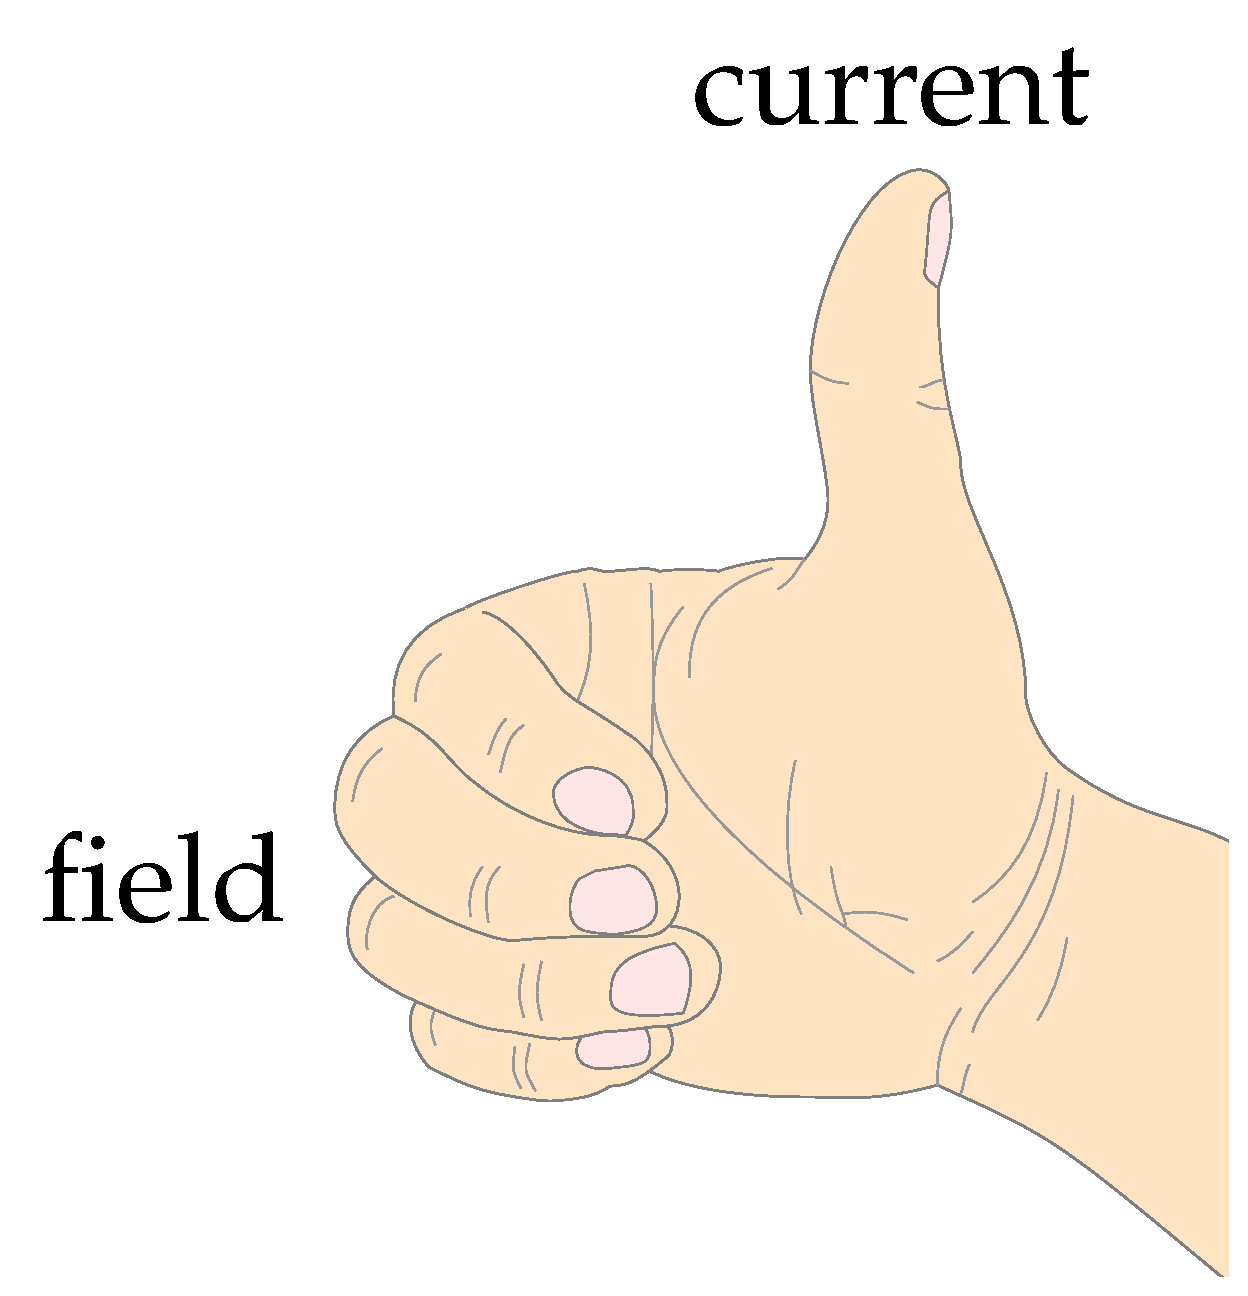
\includegraphics[height=108pt]{right-hand-straight.pdf}
\end{center}
\end{minipage}

\caption{field due to a long straight current-carrying wire}
\end{figure}

\begin{figure}[ht]
	\centering
\begin{minipage}{0.3\linewidth}
	\begin{center}
		\begin{tikzpicture}[scale=0.9,decoration={markings,mark=at position 0.75 with {\arrow{>}}}]
		\draw[very thick, postaction={decorate}] (0,0) ellipse (1.0 and 0.5);
		\draw (1.6,-0.5) node {current};
		\draw[white,fill] (-0.15,0.4) rectangle (0.15,0.6);
		\draw[white,fill] (-0.6,0.3) rectangle (-0.4,0.5);
		\draw[white,fill] (0.6,0.3) rectangle (0.4,0.5);
		\draw [very thick, blue, postaction={decorate}] (0,-2.4) -- (0,-0.7) (0,0) -- (0,2);
		\draw [very thick, blue, postaction={decorate}] (0.96,-2.4) [out=120,in=-84] to (0.54,-0.7) (0.5,0) [out=90,in=-110] to (0.9,2);
		\draw [very thick, blue, postaction={decorate}] (-0.96,-2.4) [out=60,in=-96] to (-0.54,-0.7) (-0.5,0) [out=90,in=-70] to (-0.9,2);
		\draw [very thick, blue, dashed] (0,-0.7) -- (0,-0.1);
		\draw [very thick, blue, dashed] (0.54,-0.7) [out=96,in=-90] to (0.5,0);
		\draw [very thick, blue, dashed] (-0.54,-0.7) [out=84,in=-90] to (-0.5,0);
		\draw (1.4,1.5) node {field};
		\end{tikzpicture}
	\end{center}
\end{minipage}
\begin{minipage}{0.4\linewidth}
	\begin{center}
		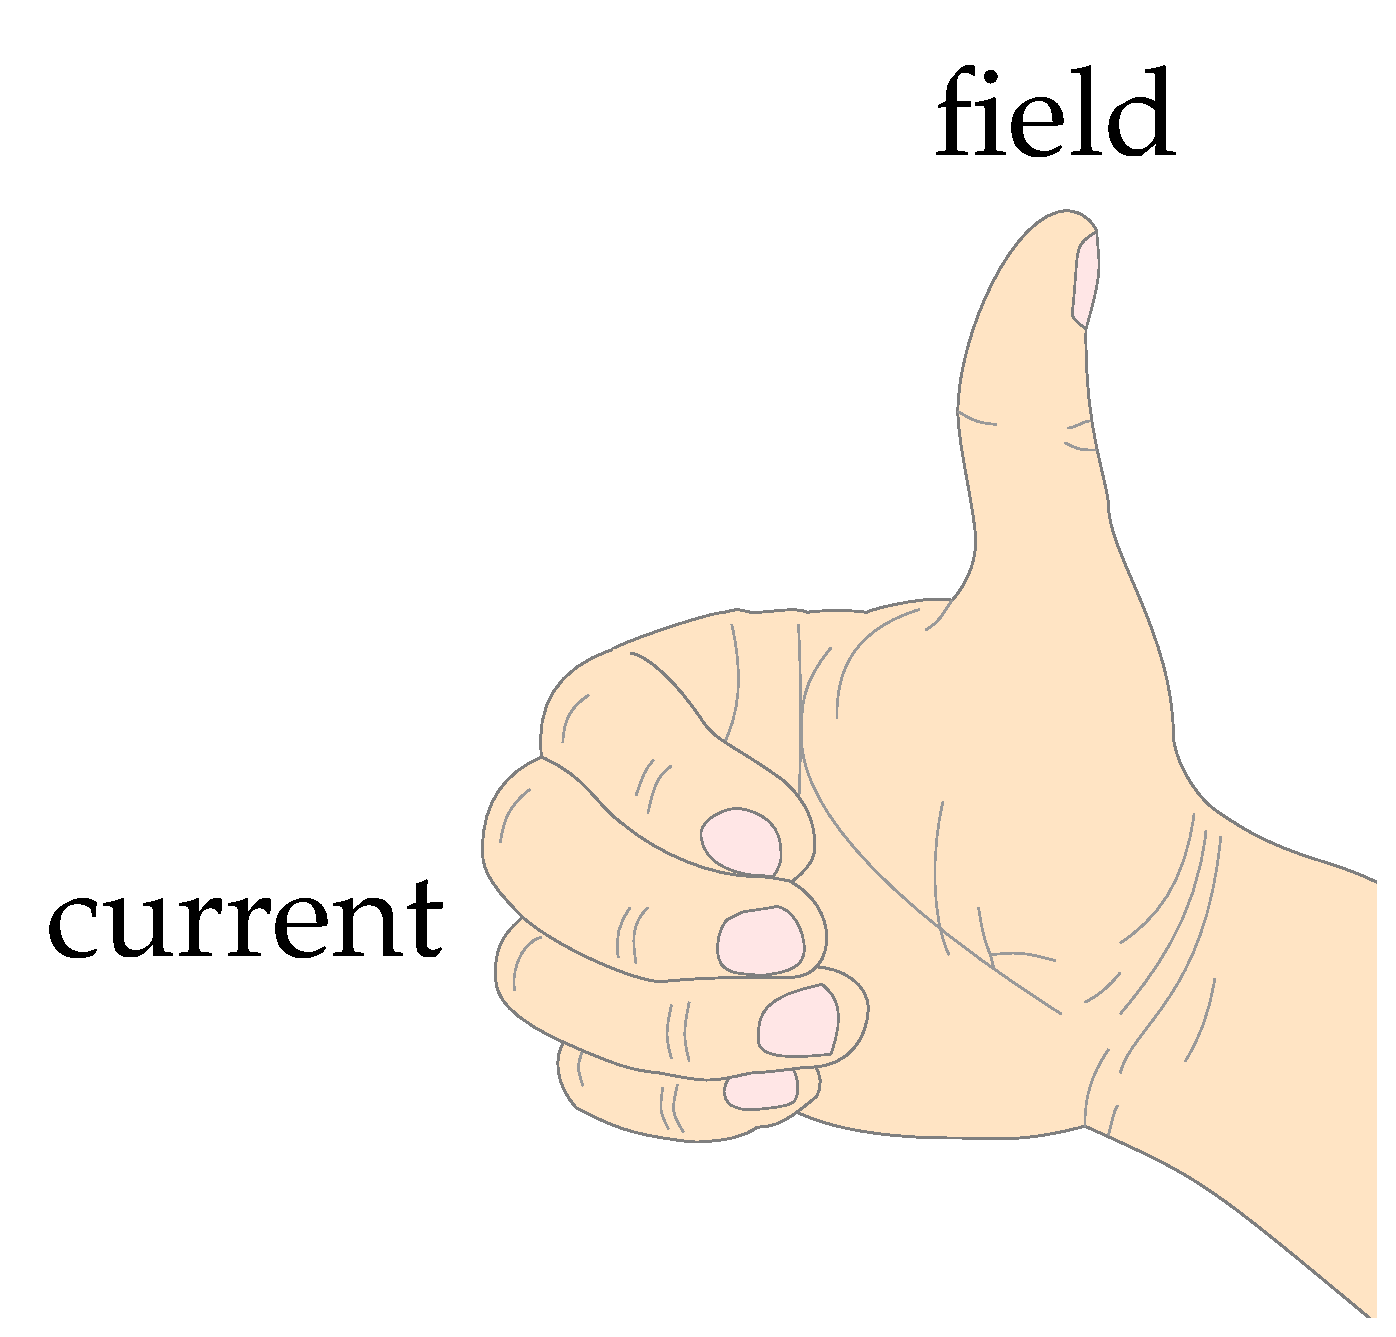
\includegraphics[height=120pt]{right-hand-circular.pdf}
	\end{center}
\end{minipage}

\caption{field due to a circulating current}
\end{figure}

\cmt strength of the field is proportional to the current: $B \propto I$

for both straight wires The magnetic flux density generated by a current flowing in an infinitely long wire in free space is given by: $\tcbhighmath{B=\frac{\mu_0 I}{2\pi r}}$, $I$ is the electric current, $r$ is the perpendicular distance from the current, and $\mu_0 = 4\pi \times 10^{-7} \text{ T m A}^{-1}$ is a fundamental physical constant called the \emph{vacuum permeability}.

 and coils, greater current means stronger field
 The magnetic flux density at the centre of a current-carrying coil in free space is given by: $\tcbhighmath{B=\frac{\mu_0 NI}{L}}$, where $N$ is the number of turns, $I$ is the electric current flowing through the coil, $L$ is the length of coil, and $\mu_0$ is the vacuum permeability
 
 
\cmt strength of magnetic field can be increased with \emph{soft iron}

this is because \emph{ferromagnetic materials} (iron, cobalt, nickel) can attract magnetic field lines\footnote{If the straight wire is immersed in a material with \emph{relative permeability} $\mu_r$, then the field becomes: $B=\frac{\mu_0 \mu_r I}{2\pi r}$. Similarly, if a material with relative permeability $\mu_r$ is present, then the magnetic flux density inside a coil becomes: $B=\frac{\mu_0 \mu_r NI}{L}$. A good magnetic material (high permeability material), such as iron, has large $\mu_r$, and therefore can greatly intensify the magnetic field. \piste}

\subsection{solenoids \& electromagnets}

strength and polarity of the field due to a coil can be changed easily by tuning currents, so coils are widely used to create magnetic fields where needed

a current-carrying coil is also called a \keypoint{solenoid}

\begin{figure}[htp]
	\centering
	\begin{minipage}{0.65\linewidth}
		\begin{center}
			\begin{tikzpicture}[yscale=0.6,xscale=0.7]
			\tikzstyle flines=[thick,blue,postaction={decorate},decoration={markings,mark=at position 0.56 with {\arrow{>}}}] % field line style
			\tikzstyle ct=[very thick,postaction={decorate},decoration={markings,mark=at position 0.54 with {\arrow{>}}}] % coil style
			
			\draw [flines] (3,0) -- (6.8,0);
			\draw [flines] (3,0.2) [out=10,in=210] to (6.5,1.35);
			\draw [flines] (3,-0.2) [out=-10,in=-210] to (6.5,-1.35);
			\draw [flines] (3,0.5) [out=20,in=240] to (6,3.5);
			\draw [flines] (3,-0.5) [out=-20,in=-240] to (6,-3.5);
			
			\draw [flines] (3,0.9) [out=60,in=0] to (0,3.6) [out=180,in=120] to (-3,0.9);
			\draw [flines] (3,-0.9) [out=-60,in=0] to (0,-3.6) [out=180,in=-120] to (-3,-0.9);
			\draw [flines] (2.5,1) [out=150,in=30] to (-2.5,1);
			\draw [flines] (2.5,-1) [out=-150,in=-30] to (-2.5,-1);
			\draw[ct] (-2.6,-3.5) --++ (0,3);
			
			\draw[thick,fill=white] (3,0) ellipse (0.35 and 1);
			\draw[thick,white,fill] (-3,-1) rectangle (3,1);
			\draw[thick,fill=white] (-3,0) ellipse (0.35 and 1);
			\draw[thick] (-3,-1) -- (3,-1);
			\draw[thick] (-3,1) -- (3,1);
			\foreach \k in {-2.5,-2.0,...,2.1} {\draw[ct] (\k,1) [out=60, in=-120] to (\k+0.4,-1);}
			\draw[very thick] (2.5,1) [out=60, in=-120] to (2.9,-1);
			\draw[white,fill] (2.6,-.978) rectangle (2.8,0);
			\draw[white,fill] (2.7,-1.1) rectangle (2.9,-1.022);
			\draw[very thick] (2.7,0.1) -- (2.7,-1);
			\draw[ct] (2.7,-1) --++ (0,-2.5);
			
			\draw [flines] (-6.8,0) -- (-3,0);
			\draw [flines] (-6.5,1.35) [out=-30,in=170] to (-3,0.2);
			\draw [flines] (-6.5,-1.35) [out=30,in=190] to (-3,-0.2);
			\draw [flines] (-6,3.5) [out=-60,in=160] to (-3,0.5);
			\draw [flines] (-6,-3.5) [out=60,in=200] to (-3,-0.5);
			
			\draw (2.8,-2.1) --++ (1.2,-0.8) node[below]{current};
			\node at (5.4,1.2) {field};
			\node at (3.6,1.4) {N};
			\node at (-3.6,1.4) {S};
			\end{tikzpicture}
		\end{center}
	\end{minipage}
	\begin{minipage}{0.3\linewidth}
		\begin{center}
		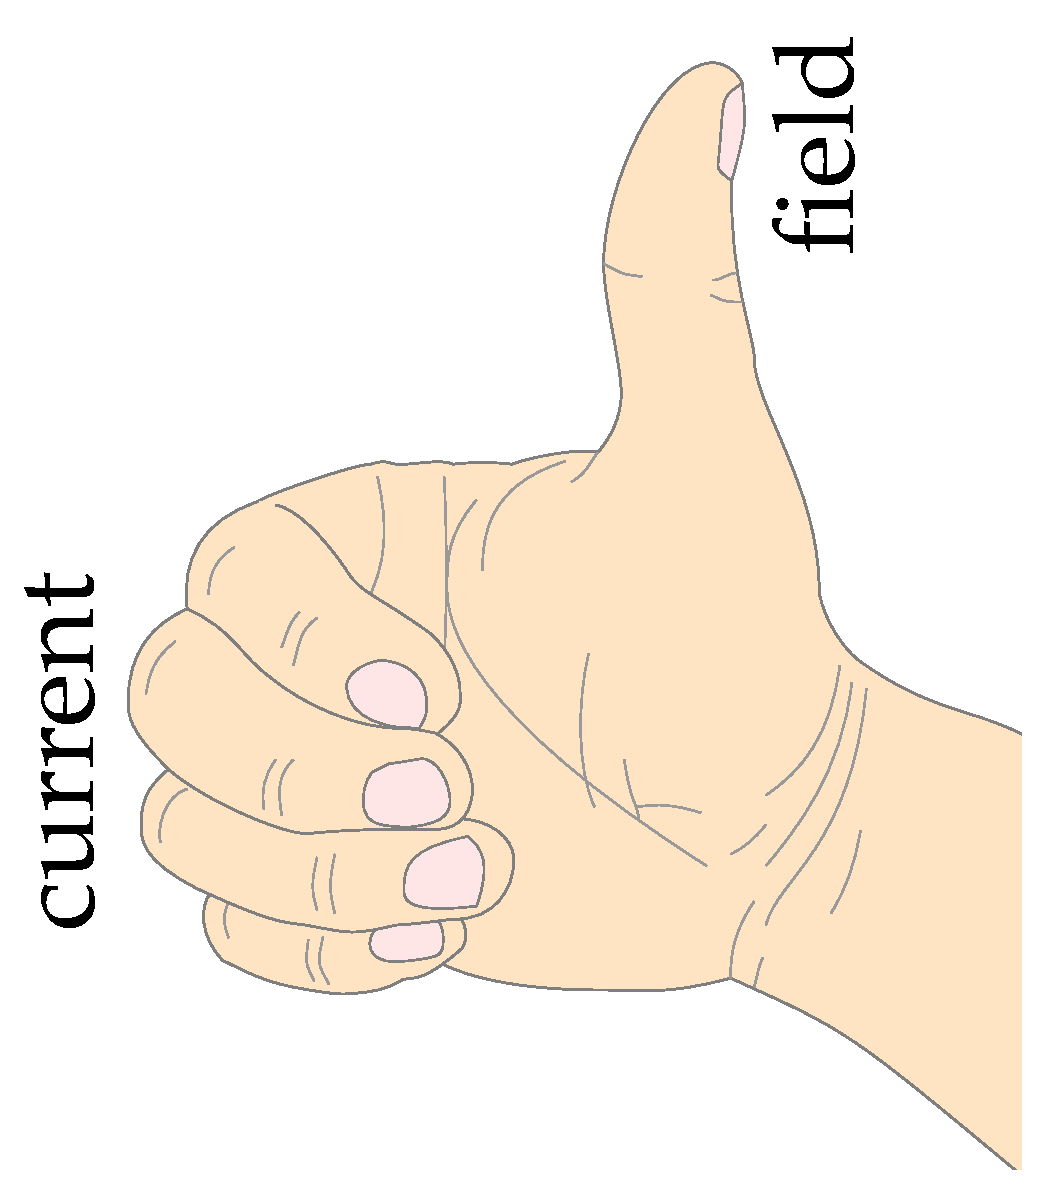
\includegraphics[height=120pt,angle=-90]{right-hand-coil.pdf}
		\end{center}
	\end{minipage}
	
	\caption{magnetic field around a solenoid}
\end{figure}

\cmt a solenoid generates a magnetic field similar to that of a bar magnet

useful to talk about the north and south poles of a solenoid

\cmt direction of magnetic field in a solenoid is given by the \keypoint{right-hand (grip) rule}\index{right-hand rule}

%\cmt a solenoid produces a \emph{uniform} magnetic field in its centre and near its poles

\cmt magnetic field produced by a solenoid can be controlled

current $I\up \ra $ stronger field, also number of turns $N\up\ra $ stronger field

\cmt inserting an \emph{iron core} inside greatly strengthens the field, this makes an \emph{electromagnet}

\question{Describe the magnetic field due to an alternating current through a solenoid.}


\subsection{magnetic force on current-carrying conductor}

\subsection{magnetic force on current-carrying conductor}

a current-carrying wire produces its own magnetic field, when it is surrounded by an external magnetic field, the two fields would interact $\Rightarrow$ a \keypoint{magnetic force}\index{magnetic field!magnetic force} on the conductor

\begin{marginfigure}
	\vspace*{-16pt}
	\centering
	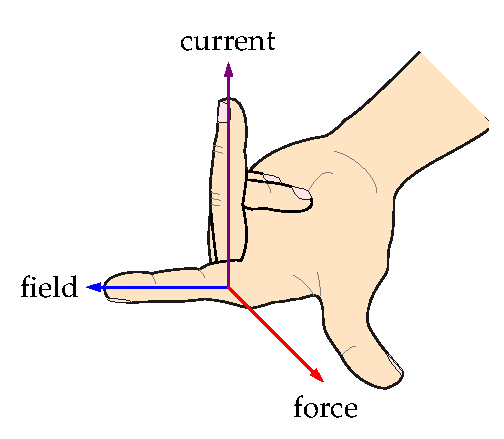
\includegraphics[height=135pt]{left-hand.pdf}
	
	Fleming's left-hand rule
	\vspace*{-16pt}
\end{marginfigure}

\cmt direction of magnetic force on current can be worked out with \keypoint{Fleming's left-hand rule}\index{left-hand rule}\footnote[][2cm]{Figure credit again goes to \emph{Thomas S\"{o}ll} from the CTAN community.}

\cmt magnitude of magnetic force: $\tcbhighmath{F=BIL\sin\theta}$

$B$ is the magnetic flux density to be specified later

$I$ is the current, $\theta$ is the angle between $B$ and $I$

\cmt when $B \perp I$, magnetic force $F=BIL$

when $B \parallelslant I$, there is no magnetic force

when $B$ forms angle $\theta$ with $I$, only the \emph{perpendicular}

\noindent\emph{component} contributes to the force, giving rise to the $\sin\theta$ factor in the formula

\cmt magnetic force is perpendicular to both $B$ and $I$
\footnote{Vector form of the formula: $\vec{F} = l\vec{I} \times \vec{B}$. \piste}

\example{Determine the direction of the magnetic force acting. Check yourself.}
\begin{center}
	\begin{minipage}[b]{0.32\textwidth}
		\centering
		\begin{tikzpicture}[scale=0.45]
		\foreach \y in {-2,2} \foreach \x in {-2,2}
		\node at (\x,\y) {\large\textcolor{blue}{$\times$}};
		%magnetic fields
		\draw[ultra thick,->] (-3.5,0) -- (2,0) node[below]{\textcolor{black}{$I$}} ;
		\draw[ultra thick] (2,0) -- (3.5,0); %currents
		\draw[red,very thick,->] (0,0) -- (0,2.4) node[right]{$F$};
		\node[blue,above right] at (2,2) {$B$};
		\end{tikzpicture}
		
		(a)
	\end{minipage}
	\begin{minipage}[b]{0.32\textwidth}
		\centering
		\begin{tikzpicture}[scale=0.4]
		\foreach \y in {-2,2} \foreach \x in {-2,2}
		\draw[blue,fill] (\x,\y) circle(0.1);
		%magnetic fields
		\draw[ultra thick,->] (0,-3.5) -- (0,2) node[right]{\textcolor{black}{$I$}} ;
		\draw[ultra thick] (0,2) -- (0,3.5); %currents
		\draw[red,very thick,->] (0,0) -- (2.4,0) node[below]{$F$};
		\node[blue,above right] at (2,2) {$B$};
		\end{tikzpicture}
		
		(b)
	\end{minipage}
\begin{minipage}[b]{0.32\textwidth}
	\centering
	\begin{tikzpicture}[scale=0.64,decoration={markings,mark=at position 0.84 with {\arrow{>}}}]
	\foreach \y in {-2,2}
	{
		\draw[blue,thick,postaction={decorate}] (-3,\y) -- (3,\y);
	}
	%magnetic fields
	\node[blue] at (3.4,1) {$B$};
	\draw [very thick, postaction={decorate}] (-2,0) -- ++(0:4) node[right] {$I$};
	\node[red,below] at (0,-0.3) {$F=0$};
	\end{tikzpicture}
	
	(c)
\end{minipage}
\end{center}


\subsection{magnetic flux density} \label{sec:magnetic_flux_density}

rewrite $F=BIL\sin\theta$ as $B = \frac{F}{IL\sin\theta}$,we can now give a formal definition for flux density $B$:

\begin{ilight}
	\keypoint{magnetic flux density}\index{magnetic field!magnetic flux density} $B$ at a point is defined as the force acted per unit length on a conductor carrying a unit current at right angle to the magnetic field
\end{ilight}

\cmt flux density describes the strength of a magnetic field\footnote{Magnetic field strength is a different quantity, defined by $H=\frac{B}{\mu}$, with $\mu=\mu_0\mu_r$ being the \emph{magnetic permeability} of material. The naming of field strength $H$ and flux density $B$ are due to historical reasons.}

\cmt $B$ is measured in \keypoint{tesla}\index{tesla} (T)\footnote{Telsa is a very large unit. For example, the strength of a typical refrigerator magnet is of about $10^{-3} \text{ T}$, even the very strong superconducting coils used in MRI are of around $1\sim3 \text{ T}$.}: $[B]=\text{T}$, $1 \text{ T} = 1 \text{ N}\cdot\text{A}^{-1}\cdot\text{m}^{-1}$

\begin{ilight}
	if a wire of 1 m normal to the magnetic field that carries a current of $1\text{ A}$ experiences a force of $1\text{ N}$, then the magnetic flux density is $1\text{ T}$
\end{ilight}

\cmt $B$ is a \emph{vector} quantity, with both magnitude and direction


\example{A wire of 0.80 m carrying a current of 5.0 A is lying at right angles to a magnetic field, it experiences a force of 0.60 N, what is the flux density?}
	
\begin{soln} $B=\frac{F}{IL} = \frac{0.60}{5.0\times0.80} = 0.15 \text{ T} \quad $ (a field of over 0.1 T is actually quite strong!) \end{soln}


\newpage
\example{Torque on a rectangular metal frame in uniform magnetic field}

\begin{marginfigure}
	\vspace*{-12pt}
	\centering
	\begin{tikzpicture}[scale=0.96,decoration={markings,mark=at position 0.75 with {\arrow{>}}}]
	\draw[very thick, postaction={decorate}] (0,0) -- (0,3);
	\draw[very thick, postaction={decorate}] (0,3) -- (2,3);
	\draw[very thick, postaction={decorate}] (2,3) -- (2,0);
	\draw[very thick,postaction={decorate}] (0.8,-1.4) -- (0.8,0) -- (0,0);
	\draw[very thick,postaction={decorate}] (2,0) -- (1.2,0) --++ (0,-1.4);
	\foreach \y in {0.5,2.5} {
		\draw[blue,thick,->] (-1,\y) -- (3,\y);
	}
	\node[above,blue] at (3,2.5) {$B$};
	\node[below left] at (0,0) {$P$};
	\node[above left] at (0,3) {$Q$};
	\node[above right] at (2,3) {$R$};
	\node[below right] at (2,0) {$S$};
	\node[right] at (2,1) {$I$};
	\node[right,red] at (2.1,1.5) {$F$};
	\node[left,red] at (-0.1,1.5) {$F$};
	
	\draw[thick,<->] (-1.5,0) --++ (0,3) node[left, midway]{$L$};
	\draw[thick,<->] (0,3.6) --++ (2,0) node[midway,above]{$d$};
	
	\draw[white,fill] (2,1.5) circle (0.18);
	\draw[white,fill] (0,1.5) circle (0.18);
	\draw[red,thick] (2,1.5) circle (0.18);
	\draw[red,thick,fill] (2,1.5) circle (0.06) (0.6,1.3) node[above right]{$I$};
	\draw[red,thick] (0,1.5) circle (0.18);
	\draw[red,very thick] (-0.1,1.4) -- (0.1,1.6) (-0.1,1.6) -- (0.1,1.4);
	\end{tikzpicture}
	\vspace*{-8pt}
\end{marginfigure}

a rectangular frame lies in parallel with the field

$QR, PS \parallelslant B$, so no force acting on these two sides

$PQ, RS \perp B$, so there is magnetic force $F=BIL$

using left-hand rule, we find $F_{PQ}$ acts into the paper, $F_{RS}$ acts out of the paper

this is a pair of equal but opposite forces

they produce a torque about central axis of frame: $\tau=Fd=BILd$, causing the frame to rotate\footnote{This effect allows engineers to build \emph{electric motors}, such as those in electric vehicles, washing machines, blenders, etc.}\eoe

\question{If the plane of the rectangular frame is at right angle to the magnetic field, describe the magnetic forces acting on each side and hence state what happens to the frame.}

\begin{marginfigure}
	\vspace*{-12pt}
	\centering
	\begin{tikzpicture}[scale=0.75]
	\draw[ultra thick] (-2.5,0) -- (-2.5,4) --++ (1,0) --++ (0,-3) --++ (3,0) --++ (0,3) -- (2.5,4) -- (2.5,0) -- cycle;
	\node at (0,4) {\large $\otimes$};
	\node[above] at (0,4.1) {$I$};
	\node at (2,3.6) {$N$};
	\node at (-2,3.6) {$S$};
	\draw[ultra thick] (-3,-2) rectangle (3,-0.1);
	\draw[thick] (-1.5,-1.6) rectangle (1.5,-0.5);
	\node at (0,-1.1) {\large 500.0 g};
	\end{tikzpicture}
	\vspace*{-12pt}
\end{marginfigure}

\example{A U-shaped magnet is placed on a balance with a wire suspended above it as shown. Magnetic flux density between the poles is about 0.50 T. The part of the wire that is in the field is of length 8.0 cm. The balance initially shows a reading of 500.0 g. When a current of 10 A flowing into the paper is switched on, what is the new reading on the balance?}\label{ex-mag-balance}

\sol use left-hand rule, force on wire acts upwards

from \emph{Newton's third law}, reaction force on magnet acts downwards

so there will be an increase in the balance reading

magnitude of the force: $F=BIl = 0.50 \times 10 \times 8.0\times10^{-2} = 0.40 \text{ N}$

change in the mass reading: $\Delta m = \frac{F}{g} = \frac{0.40}{9.81} \approx 0.0407 \text{ kg} \approx 40.7 \text{ g}$

new reading on balance: $m_\text{new} = 500.0 + 40.7 = 540.7 \text{ g}$ \eoe

\question{If the current in Example \ref{ex-mag-balance} is replaced by a current of 6.0 A flowing out of the plane of the paper. What is the reading on the balance?}

\subsection*{force between long straight current-carrying wires}

\begin{center}
\begin{minipage}{0.3\linewidth}
\begin{center}
\begin{tikzpicture}[scale=0.84,decoration={markings,mark=at position 0.6 with {\arrow{>}}}]
\draw[ultra thick, postaction={decorate}] (-1.2,0) node[left]{$I_1$} (-1.2,-2) -- (-1.2,2);
\draw[ultra thick, postaction={decorate}] (1.2,0) node[right]{$I_2$} (1.2,-2) -- (1.2,2);
\end{tikzpicture}
\end{center}
\end{minipage}
\begin{minipage}{0.35\linewidth}
\begin{center}
\begin{tikzpicture}[scale=0.56,decoration={markings,mark=at position 0.4 with {\arrow{>}}}]
\draw[black,thick] (0,0) circle (0.25);
\draw[black,thick,fill] (0,0) circle (0.06) (0,0.2) node[above]{$I_1$};
\draw[black,thick] (3,0) circle (0.25);
\draw[black,thick,fill] (3,0) circle (0.06) (3,0.2) node[above left]{$I_2$};
\draw[thick, blue, postaction={decorate}] (4:3) arc [radius=3, start angle=5, end angle=356];
\draw[blue] (144:3.6) node{$B_1$};
\draw[red,thick,->] (3,0) -- (1.2,0) node[below]{$F_{21}$};
\end{tikzpicture}
\end{center}
\end{minipage}
\begin{minipage}{0.3\linewidth}
\begin{center}
\begin{tikzpicture}[scale=0.84,decoration={markings,mark=at position 0.6 with {\arrow{>}}}]
\draw[ultra thick, postaction={decorate}] (-1.2,0) node[left]{$I_1$} (-1.2,-2) -- (-1.2,2);
\draw[ultra thick, postaction={decorate}] (1.2,0) node[right]{$I_2$} (1.2,-2) -- (1.2,2);
\draw[red,thick,->] (1.2,0) -- (0.1,0) node[below right]{$F_{21}$};
\draw[red,thick,->] (-1.2,0) -- (-0.1,0) node[below left]{$F_{12}$};
\end{tikzpicture}
\end{center}
\end{minipage}
\end{center}

if we have two straight parallel wires carrying currents in the same direction

force acting on $I_2$ is due to magnetic field $B_1$ generated by $I_1$

from top view, $I_1$ creates a counter-clockwise $B_1$, so $I_2$ experiences an upward field

using left-hand rule, force acting on $I_2$ by $I_1$, denoted $F_{21}$\footnote{$F_{AB}$ denotes the force acted on object $A$ by object $B$.}, points to the left

since $F_{21}$ and $F_{12}$ are a pair of action-reaction, so $F_{12}$ points to the right


\begin{center}
\begin{minipage}{0.3\linewidth}
\begin{center}
\begin{tikzpicture}[scale=0.84,decoration={markings,mark=at position 0.6 with {\arrow{>}}}]
\draw[ultra thick, postaction={decorate}] (-1.2,0) node[left]{$I_1$} (-1.2,-2) -- (-1.2,2);
\draw[ultra thick, postaction={decorate}] (1.2,0) node[right]{$I_2$} (1.2,2) -- (1.2,-2);
\end{tikzpicture}
\end{center}
\end{minipage}
\begin{minipage}{0.35\linewidth}
\begin{center}
\begin{tikzpicture}[scale=0.56,decoration={markings,mark=at position 0.4 with {\arrow{>}}}]
\draw[black,thick] (0,0) circle (0.25);
\draw[black,thick,fill] (0,0) circle (0.05) (0,0.2) node[above]{$I_1$};
\draw[black,thick] (3,0) circle (0.25);
\draw[black,thick] (3,0.2) node[above left]{$I_2$};
\draw[black,thick] (3.13,0.13) -- (2.87,-0.13) (3.13,-0.13) -- (2.87,0.13);
\draw[thick, blue, postaction={decorate}] (4:3) arc [radius=3, start angle=5, end angle=356];
\draw[blue] (144:3.6) node{$B_1$};
\draw[red,thick,->] (3,0) -- (4.8,0) node[below]{$F_{21}$};
\end{tikzpicture}
\end{center}
\end{minipage}
\begin{minipage}{0.3\linewidth}
\begin{center}
\begin{tikzpicture}[scale=0.84,decoration={markings,mark=at position 0.6 with {\arrow{>}}}]
\draw[ultra thick, postaction={decorate}] (-1.2,0) node[right]{$I_1$} (-1.2,-2) -- (-1.2,2);
\draw[ultra thick, postaction={decorate}] (1.2,0) node[left]{$I_2$} (1.2,2) -- (1.2,-2);
\draw[red,thick,->] (1.2,0) -- (2.2,0) node[below left]{$F_{21}$};
\draw[red,thick,->] (-1.2,0) -- (-2.2,0) node[below right]{$F_{12}$};
\end{tikzpicture}
\end{center}
\end{minipage}
\end{center}

similar discussions apply for $I_1$ and $I_2$ flowing in opposite directions (left as exercise)

hence we come to an conclusion: \emph{parallel currents attract, and anti-parallel currents repel}\footnote{The S.I. unit for current, ampere, is defined using two long wires parallel to each other carrying the same current in the same direction. If the wires are separated by 1 m and the magnetic force experienced per metre is $2.0\times10^{-7}$ N, then the current is of 1 A.}

\question{A light coil of wire of several loops is suspended from a fixed point. When an electric current is switched on in the coil, state and explain the change in the separation between the loops.}

\question{Two long parallel wires carry currents of $I_1=$3.0 A and $I_2=$5.0 A in the same direction as shown. The flux density at a point at perpendicular distance $r$ from a straight long wire carrying current $I$ is given by $B=\frac{\mu_0 I}{2\pi r}$.}\label{q-pwires}



\begin{figure}[htp]
\centering
\begin{tikzpicture}[scale=1.2,decoration={markings,mark=at position 0.65 with {\arrow{>}}}]
\draw[very thick, postaction={decorate}] (0,0) --++ (0,4) node[pos=0.55, left]{$I_1$};
\draw[very thick, postaction={decorate}] (3,0) --++ (0,4) node[pos=0.55, left]{$I_2$};
\draw[gray,dashed,thick] (-2.5,1) --++ (1.5,2) --++ (6.5,0) --++ (-1.5,-2) --++ (-6.5,0); 
\end{tikzpicture}
\end{figure}

\begin{compactenum}
\item[(a)] Draw at least three lines to show the magnetic field due to $I_1$.

\item[(b)] State and explain the direction of force acting on $I_2$.

\item[(c)] Given that $I_1$ and $I_2$ are separated by 4.0 cm, what is flux density due to $I_1$ at $I_2$?

\item[(d)]  What is the magnetic force per unit length acting on $I_2$?

\item[(e)] What is the magnitude and the direction of the force per unit length acting on $I_1$?
	
\end{compactenum}

\question{If the current in one of the two wires in Question \ref{q-pwires} is replaced by an alternating current, then the two wires should begin to vibrate. However, the wires are not observed to move. Make some reasonable estimates and explain why the vibration is not observed.}







\subsection{magnetic force on charged particles}

electric currents are formed by moving charges, since current-carrying wires in a magnetic field experience force, charged particle moving in magnetic field should also experience force

\subsection{magnetic force on charged particles}

starting from $F=BIl\sin\theta$, let's substitute $I=nAqv \RA F=B(nAqv)l\sin\theta$

notice $n$ is the number density of charged particles, so $nAl$ together gives the total number

if we look at the force acting on \emph{one} charged particle, then $nAl=1$, so: $F=Bqv\sin\theta$\index{magnetic field!magnetic force}

\cmt magnitude of magnetic force on charged particle: $\tcbhighmath{F=Bqv\sin\theta}$ 

$B$ is magnetic flux density, $q$ is electric charge of the particle, $v$ is its velocity

$\theta$ refers to the angle between $B$ and $v$

\begin{marginfigure}
	\vspace*{-16pt}
	\centering
	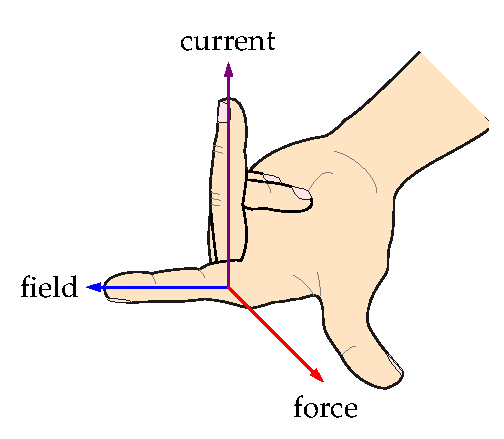
\includegraphics[height=135pt]{left-hand.pdf}
	
	Fleming's left-hand rule
	\vspace*{-16pt}
\end{marginfigure}

\cmt direction of magnetic force can be determined using \emph{Fleming's left-hand rule}\index{left-hand rule}

for $+q$, current in same direction as $v$

for $-q$, current in opposite direction as $v$

\cmt force depends on \emph{perpendicular component} of $B$

if $v \perp B$, magnetic force $F=Bqv$

if $v \parallelslant B$, there is no magnetic force

when particle moves at angle $\theta$ to $B$, contribution to the force only comes from the \emph{perpendicular component}, giving rise to the $\sin\theta$ factor

\cmt magnetic force always perpendicular to both velocity $v$ and magnetic field $B$\footnote{Vector form of the formula: $\vec{F} = q\vec{v} \times \vec{B}$. \piste}

\example{Use the left-hand rule to find the direction of the magnetic forces acting on the following moving charges. Check yourself.}
\begin{figure*}
	\begin{minipage}[b]{0.45\textwidth}
		\centering
		\begin{tikzpicture}[scale=1]
		\draw[blue,dashed] (-2.7,-2.7) rectangle (2.7,2.7);
		\foreach \y in {-2,0,2} \foreach \x in {-2,0,2}
		\node at (\x,\y) {\large\textcolor{blue}{$\times$}};
		%magnetic fields
		\draw[purple,very thick,->] (-1.1,-1.2) --++ (1.5,0) node[midway,above]{$v$};
		\draw[red,very thick,->] (-1.1,-1.2) --++ (0,1.8) node[left]{$F$};
		\shade [ball color = orange] (-1.1,-1.2) circle (0.15);
		\node[below] at (-1.1,-1.4) {$+q$};
		\draw[purple,very thick,->] (1.2,1.2) --++ (0,-1.5) node[midway,right]{$v$};
		\draw[red,very thick,->] (1.2,1.2) --++ (-1.8,0) node[above]{$F$};
		\shade [ball color = green] (1.2,1.2) circle (0.15);
		\node[above] at (1.2,1.4) {$-q$};
		\node[blue,above right] at (2,2) {$B$};
		\end{tikzpicture}
		
		(a)
	\end{minipage}
	\begin{minipage}[b]{0.45\textwidth}
		\centering
		\begin{tikzpicture}[scale=1]
		\draw[blue,dashed] (-2.7,-2.7) rectangle (2.7,2.7);
		\foreach \y in {-2,0,2} \foreach \x in {-2,0,2}
		\draw[blue,fill] (\x,\y) circle(0.05);
		%magnetic fields
		\draw[purple,very thick,->] (-0.6,-1.2) --++ (110:1.4) node[midway,above right]{$v$};
		\draw[red,very thick,->] (-0.6,-1.2) --++ (20:1.8) node[below]{$F$};
		\shade [ball color = orange] (-0.6,-1.2) circle (0.15);
		\node[below] at (-0.6,-1.4) {proton};
		\draw[purple,very thick,->] (1,0.5) --++ (70:1.2) node[midway,right]{$v$};
		\draw[red,very thick,->] (1,0.5) --++ (160:1.8) node[above]{$F$};
		\shade [ball color = green] (1,0.5) circle (0.15);
		\node[below] at (1,0.3) {electron};
		\node[blue,above right] at (2,2) {$B$};
		\end{tikzpicture}
		
		(b)
	\end{minipage}
\end{figure*}

\subsection*{charged particles in electric \& magnetic fields}

in either electric field or magnetic field, charged particle may experience a force\footnote{The combination of electric and magnetic force on the charge due to electromagnetic fields is called the \emph{Lorentz force}\index{Lorentz force}: $\vec{F} = q(\vec{E} + \vec{v}\times \vec{B})$. If you have a good knowledge in maths, everything we cover in this section can be recovered from this vector equation. \piste}

in this section, we will compare the difference between electric field and magnetic field

\begin{center}
	{%\renewcommand{\arraystretch}{1.2}
		\begin{tabular}{|D{0.22\textwidth}|D{0.36\textwidth}|D{0.3\textwidth}|}
			
			\hline
			& electric field & magnetic field \\ \hline
			
			strength of the field & electric field strength $E$ & magnetic flux density $B$ \\ \hline
			
			magnitude of force & $F_E = Eq$ & $F_B=Bqv\sin\theta$ \\ \hline
			
			whether force depends on velocity & no dependence, acts equally on stationary or moving charges & depend on perpendicular component of velocity \\ \hline
			
			\multirow{2}{*}{direction of force} & $F_E \parallelslant E$ &  $F_B \perp B$ and $F_B \perp v$ \\
			
			& same as/opposite to $E$ for $+q$/$-q$ & use left-hand rule\\ \hline
			
			effect of force on motion of particle & can change both magnitude and direction of velocity & only changes direction of velocity, cannot change magnitude of velocity \\ \hline
			
			work done by force & work can be done, can define notions of potential and P.E. & magnetic force does no work for charged particles\\ \hline
			
	\end{tabular}}
\end{center}



\subsection{charged particle in uniform magnetic fields}

suppose a charged particle is moving at right angle to a uniform magnetic field

\begin{figure}[htp]
	\centering
	\begin{tikzpicture}[scale=0.65]
			\draw[blue, dashed] (-4,-4) rectangle (4,4);
			\foreach \x in {-3,0,3}{
				\foreach \y in {-3,0,3}{
					\node[draw,circle,blue,inner sep=0.8pt,fill] at (\x,\y) {};  }}
			\node[blue] at (-2.5,2.5) {$B$};
			\draw[thick,dotted] (0,0) circle [radius=2.5];
			\foreach \s in {80,200,310}
			{
				\draw [purple, thick, ->] (\s:2.5) -- ++(\s-90:2);
				\draw [purple] (\s-35:3.5) node{$v$};
				\draw [red, thick, ->] (\s:2.5) -- (\s:0.8);
				\draw [red] (\s+25:1) node{$F$};
				\shade [ball color = yellow] (\s:2.5) circle (0.25) node{\footnotesize$+$};
			}
	\end{tikzpicture}
	
	circular motion of a charged particle in uniform magnetic field
\end{figure}

magnetic force $F_B$ always at right angle to motion, so $F_B$ keeps changing direction of velocity

uniform field means a constant force, so $F_B$ deflects the particle at the same rate

the particle should describe a \emph{circular} path!

\begin{ilight}
	for a charged particle moving in a uniform magnetic field, \emph{magnetic force provides centripetal force for circular motion}: $\tcbhighmath{Bqv = \frac{mv^2}{r}}$, or $\tcbhighmath{Bqv = m \omega^2 r}$
\end{ilight}

\cmt can solve for radius of the orbiting particles: $r=\frac{mv}{Bq}$

\begin{compactenum}

\item[-] $v\up \Rightarrow r\up$, faster particles take larger circles
	
\item[-] $B\up \Rightarrow r\down$, stronger magnetic field, larger centripetal force, smaller circles
	
\item[-] $m\up \Rightarrow r\up$, larger mass, larger inertia, so larger circles

\end{compactenum}
	
\cmt radius of curvature relates to charge-to-mass ratio (also called \emph{specific charge}\index{specific charge}) of the particle

rearrange the equation we have $\frac{q}{m}=\frac{v}{Br}$, which can be computed using experimental data

\example{An $\alpha$-particle travelling at $2.5\times10^4 \mps$ enters a region of uniform magnetic field. The field has flux density of 5.4 mT and is normal to direction of particle's velocity. What is the radius of $\alpha$-particle's path?}

\begin{soln} radius of circular arc: $r=\frac{mv}{Bq} = \frac{4\times 1.66\times10^{-27}\times2.5\times10^4}{5.4\times10^{-3}\times2\times1.60\times10^{-19}} \approx 0.096 \text{ m} \approx 9.6 \text{ cm}$ \end{soln}

\question{For an $\alpha$-particle and a $\beta$-particle entering the same uniform magnetic field at a same speed, compare the radius of their paths.}

\question{For a charged particle undergoing circular motion in a uniform magnetic field, show that its angular velocity is independent of the radius of its path.}

\question{If a charged particle enters a uniform magnetic field at an angle $\theta \neq 90^\circ$, state and explain the path of this particle. (Hint: think about components of its velocity.)}
	
\subsection{mass spectrometer}

a \keypoint{mass spectrometer}\index{mass spectrometer} is a device to measure the charge-to-mass ratio of charged particles

\begin{figure*}[ht]
	\centering
	\begin{tikzpicture}[scale=0.72,decoration={markings,mark=at position 0.7 with {\arrow{>}}}]
	% electric fields
	\draw[orange,dashed,fill=orange!20] (-8,1.5) rectangle (-4,-1.5);
	\draw[ultra thick] (-8,-1.5) --++ (0,3);
	\draw[ultra thick] (-4,-1.5) --++ (0,1.3) (-4,1.5) --++ (0,-1.3);
	\draw (-6,-1) --++ (-1.2,-1.5) node[twoline,below]{accelerating voltage\\supply of p.d. $V$};
	% magnetic field
	\draw[dashed,blue,fill=blue!10] (0,1) rectangle (5,-9);
	\node[blue] at (3.6,-0.4){$B$};
%	\foreach \y in {0.167,-1.5,-3.167,-4.833,-6.5,-8.167} \foreach \x in {0.833,2.5,4.167}
%	\node[blue] at (\x,\y) {$\times$};
	\draw (4.5,-0.5) --++ (1.2,1.2) node[twoline,right]{uniform magnetic\\field region};
	% paths of particle beam
	\draw [thick,purple,postaction={decorate}] (0,0) arc(90:-90:4);
	\draw [thick,purple,postaction={decorate}] (0,0) arc(90:-90:3);
	\draw [thick,purple,postaction={decorate}] (-8,0) -- (-4,0);
	\draw [thick,purple,postaction={decorate}] (-4,0) -- (0,0);
	\node[purple,above] at (-2,0) {$v$};
	\shade [ball color = green] (-7,0) circle (0.2);
	\shade [ball color = green] (-3,0) circle (0.2);
	\draw[<->] (-0.3,0) --++ (0,-8) node[midway,left]{$d=2r$};
	% detectors
	\draw[gray!50,fill] (-1,-5) rectangle(-0.7,-9);
	\draw (-0.85,-6.5) --++ (-1,1) node[left,twoline]{particle\\detector};
	\end{tikzpicture}
	
	\caption{deflection of two charged particles in a mass spectrometer}
\end{figure*}

charged particles accelerated through an electric field: $\frac{1}{2}mv^2 = qV$

they then enter a uniform magnetic field: $Bqv = \frac{mv^2}{r} \ra v=\frac{Bqr}{m}$ $\quad$

eliminating $v$: $v^2 = \frac{2qV}{m} = \frac{B^2 q^2 r^2}{m^2} \ra \frac{q}{m} = \frac{2V}{B^2 r^2}$

we can measure $V$, $B$, $r$ in practice, so the charge-to-mass ratio $\frac{q}{m}$ is worked out

since different particles usually have different values of $\frac{q}{m}$, so this technique is widely used to identify unknown particles

\question{In the figure above, two paths of deflected particles are shown. Give reasons why the radius of the circular path can be different.}

\question{If the particles sent into the mass spectrometer are positively-charged, in which direction should the magnetic field be applied?}

\question{A particle carrying a charge of $+e$ enters a uniform magnetic field of $8.8$ mT at right angles with an initial speed of $1.4\times10^5 \text{ m s}^{-1}$. It describes a semi-circle with diameter of 66 cm. (a) Find the mass of the particle. (b) Suggest possible composition of this particle.}

\subsection{cyclotron}\index{cyclotron}

a \keypoint{cyclotron} is a type of \emph{particle accelerator}

\begin{figure}[ht]
	\centering
	\begin{tikzpicture}[decoration={markings,mark=at position 0.6 with {\arrow{>}}}, scale=1.12]
	\def\gap{0.6}
	% magnetic fields
	\draw[thick, dashed, blue, fill=blue!10] (-2.6,0) arc(180:25:2.73) [out=-25, in = 100] to (10:3.2) arc(10:0:3.2) --cycle;
	\draw[thick, dashed, blue, fill=blue!10] (-2.6,-\gap) arc(180:360:2.9) -- cycle;
	% electric field
	\draw[thick, dashed, blue, fill=orange!20] (-2.6,0) rectangle (3.2,-\gap);
	% semi-circular paths
	\draw[thick, postaction={decorate}] (1,0) arc(0:180:1);
	\draw[thick, postaction={decorate}] (-1,-\gap) arc(180:360:1.414);
	\draw[thick, postaction={decorate}] (1.818,0) arc(0:180:1.732);
	\draw[thick, postaction={decorate}] (-1.636,-\gap) arc(180:360:2);
	\draw[thick, postaction={decorate}] (2.364,0) arc(0:180:2.236);
	\draw[thick, postaction={decorate}] (-2.108,-\gap) arc(180:360:2.449);
	% accelerating paths
	\foreach \x in {1.818,2.364,2.791} \draw[thick, postaction={decorate}] (\x,-\gap) --++ (0,\gap);
	\foreach \x in {-1, -1.636, -2.108} \draw[thick, postaction={decorate}] (\x, 0) --++ (0,-\gap);
	\draw[thick, postaction={decorate}] (2.791,0) --++(0,3);
	\draw[thick] (1,-\gap/2) --++(0,\gap/2);
	% proton source
	\draw[fill] (1,-\gap/2) circle(0.1);
	% nodes
	\draw (0.207, -\gap) ++ (200:2.6) -- (-4,0.8) (160:2.3) -- (-4,1) node[left,twoline]{magnetic field\\into the paper};
	\draw (-2.4,-\gap/2) -- (-3.6,-1) node[left,twoline]{high-frequency\\alternating\\electric field};
	\draw (1,-\gap/2) -- (3.2,-2.8) node[right,twoline]{proton\\source};
	\draw (2.791,2.2) -- (1,3.5) node[above, twoline]{outgoing beam of\\high-speed protons};
	\end{tikzpicture}
	
	\caption{protons being accelerated in a cyclotron}
\end{figure}

the idea is to makes use of magnetic force to guide moving charges into a spiral path between accelerations by an electric field

as the particle enters and leaves the region of electric field, it gains extra energy of $qV$

it then follows a semi-circular path under magnetic force and re-enters the electric field

polarity of the electric field is reversed so the particle continues to accelerate across the gap

energy of particle increases by $qV$, it then moves in a larger semi-circle in magnetic field

repeat this process, the particle leaves the exit port with very high speed



\cmt cyclotron frequency

for charged particles circulating in a uniform magnetic field: $Bqv=m\omega^2 r$

time to complete one full turn is: $T=\frac{2\pi r}{v} = \frac{2\pi}{v}\times\frac{mv}{Bq}\ra T=\frac{2\pi m}{Bq}$

this shows the period is independent of radius of the circular path!

if an alternating voltage is applied at frequency $f=\frac{Bq}{2\pi m}$, particles can be accelerated continuously at just the right time when they cross the gap

this frequency is known as the \emph{cyclotron frequency}

\question{Protons are accelerated in a cyclotron where the uniform magnetic field region has a flux density of 1.5 T and the voltage between the gap is 20 kV. (a) Find the frequency of the voltage supply needed. (b) Find the number of circles the protons must make in order to gain an energy of 10 MeV.}


\subsection{velocity selector}

\keypoint{velocity selector}\index{velocity selector} is a device to produce a beam of charged particles all with same speed $v$

\begin{figure}[ht]
	\centering
	\begin{tikzpicture}[xscale=0.9,yscale=0.8]
	\foreach \x in {-2,2}
	\foreach \y in {-1.5,1.5}
	\node[blue] at (\x,\y) {$\times$};
	\foreach \x in {-3,-1,...,3}
	\draw[orange,thick,->] (\x,3) -- (\x,-3);
	\node[blue] at (-2,2.1) {$B$};
	\node[orange] at (3.5,-2) {$E$};
	\draw[ultra thick] (-4,3) -- (4,3);
	\draw[ultra thick] (-4,-3) -- (4,-3);
	\draw[ultra thick] (0,-4.5) node[right]{$-$} -- (0,-3) (0,3) -- (0,4.5) node[right]{$+$};
	\draw [fill] (-4.2,0.2) rectangle (-4,3.6);
	\draw [fill] (-4.2,-0.2) rectangle (-4,-3.6);
	\draw [fill] (4.2,0.2) rectangle (4,3.6);
	\draw [fill] (4.2,-0.2) rectangle (4,-3.6);
	\shade [ball color = green] (-6.5,0) circle (0.1);
	\node[below,twoline] at (-6.5,-0.2) {electron\\beam};
	\draw[purple,thick,->] (-6.2,0) -- (-5,0) node[above,midway]{$v$};
	\draw[purple,thick,->] (-5,0) -- (6,0) node[above]{$v=\frac{E}{B}$};
	\draw[purple] (-4,0) [out=0,in=210] to (4,2);
	\node[purple,right] at (4.2,2) {$v<\frac{E}{B}$};
	\draw[purple] (-4,0) [out=0,in=160] to (4,-1.5);
	\node[purple,right] at (4.2,-1.5) {$v>\frac{E}{B}$};
	\shade [ball color = green] (0,0) circle (0.1);
	\draw[red,thick,->] (0,0.2) -- (0,2) node[above]{\textcolor{black}{$F_E=Eq$}};
	\draw[red,thick,->] (0,-0.2) -- (0,-2) node[below]{\textcolor{black}{$F_B=Bqv$}};
	
	\end{tikzpicture}
	
	\caption{velocity selector}
\end{figure}

let's consider a beam of electrons passing through a region where both uniform electric field and magnetic field are applied, electrons at desired speed $v$ are \emph{undeflected}

no net force acting on these electrons, so equilibrium between electric and magnetic force

{

\centering

$F_E = F_B \RA Eq = Bqv \RA \tcbhighmath{v=\frac{E}{B}}$

}

for particles entering the same region with higher speed, $F_B>F_E$, they deflect upwards

for particles entering the same region with lower speed, $F_B<F_E$, they deflect downwards

\question{If electrons at speed $v$ are undeflected when they pass through the velocity selector, what about a beam of $\alpha$-particles entering the same region at the same speed $v$?}

\question{A uniform magnetic field with flux density $6.0\times10^{-2} \text{ T}$ is applied out of the plane of the paper. A beam of protons are travelling into this region at a speed of $3.5\times10^4 \text{m s}^{-1}$. (a) In which direction do the protons deflect? (b) A uniform electric field is now applied in the same region so that the protons become undeviated. What is the strength and the direction of this electric field?}


\subsection{Hall effect}
when an electric current passes through a conductor surrounded by an external magnetic field perpendicular to the current, a transverse potential difference is produced

this phenomenon is known as the \keypoint{Hall effect}\index{Hall effect} (discovered by American physicist \emph{Edwin Hall} in 1879), the voltage difference is called the \keypoint{Hall voltage}

\vspace*{\baselineskip}

suppose magnetic field goes upward, current flows to the right (see figure), then charge carriers (assumed to be electrons for now) experience a magnetic force pointing out of paper

\begin{figure}[ht]
	\centering
	\begin{tikzpicture}[scale=1]
	\draw[thick] (-6,.5) -- ++(3,0); % current in
	\draw[thick,fill=gray!20] (-4,-1) -- ++(0,1) -- ++(3,2) -- ++(4,0) -- ++(0,-1)  -- ++(-3,-2) -- cycle;
	\draw[thick] (-4,0) -- (0,0) -- (3,2) (0,0) -- (0,-1); %conductor
	\draw[blue,thick,->] (-.5,-2.5) -- (-.5,-1) (-.5,1) -- ++(0,2) node[right]{$B$}; %magnetic fields
	\draw[thick,->] (1.5,.5) -- ++(3,0) node[above]{$I$}; % current out
	\shade [ball color = green] (-1.1,1) circle (0.12);
	\draw[thick,purple,->] (-1.1,1) -- ++(-1,0) node[above right]{$v$};
	\draw[thick,red,->] (-1.1,1) -- ++(-1,-.667) node[left]{$F_B$};
	\end{tikzpicture}
\end{figure}

this magnetic force causes a build-up of extra charge on front side of conductor, which produces an internal electric field $E$ inside conductor, i.e., a potential difference $V_H$ is formed

\begin{figure}[ht]
	\centering
	\begin{tikzpicture}[scale=1]
	\draw[thick] (-6,.5) -- ++(3,0); % current in
	\draw[thick,fill=gray!20] (-4,-1) -- ++(0,1) -- ++(3,2) -- ++(4,0) -- ++(0,-1)  -- ++(-3,-2) -- cycle;
	\draw[thick] (-4,0) -- (0,0) -- (3,2) (0,0) -- (0,-1); %conductor
	\draw[blue,thick,->] (-.5,-2.5) -- (-.5,-1) (-.5,1) -- ++(0,2) node[right]{$B$}; %magnetic fields
	\draw[thick,->] (1.5,.5) -- ++(3,0) node[above]{$I$}; % current out
	\shade [ball color = green] (-1.1,1) circle (0.12);
	\draw[thick,purple,->] (-1.1,1) -- ++(-1,0) node[above right]{$v$};
	\draw[thick,red,->] (-1.1,1) -- ++(-1,-.667) node[left]{$F_B$};
	\draw[thick,violet,->] (-1.1,1) -- ++(1,.667) node[right]{$F_E$};
	\foreach \ball in {-3.5,-2.5,-1.5,-0.5}{
		\shade [ball color = green] (\ball,-0.5) circle (0.12);
		\draw[thick] (\ball-0.05,-0.5) --++ (0.1,0);
	}
	\draw[thick,olive,<->] (-4.8,0) -- ++(3,2) node[midway,above left]{$V_H$};
	\draw[thick,olive,<-] (-0.8,.3) node[left]{$E$} -- ++(2.1,1.4);
	\draw[thick,<->] (.5,-1.35) -- ++(3,2) node[midway, below right]{$d$};
	\draw[thick,<->] (3.5,1) -- ++(0,1) node[midway, right]{$t$};
	\end{tikzpicture}
\end{figure}

as charge carriers accumulate on one side, Hall voltage opposes further migration of charges

steady $V_H$ is established when magnetic force and electric force are balanced: $Eq = Bqv$

\begin{compactenum}
	\item[-] strength of internal electric field is related to Hall voltage: $E=\frac{V_H}{d}$
	
	where $d$ is width of the conductor
	
	\item[-] drift velocity $v$ of particles is related to current $I$: $I=nAqv$
	
	where $A$ is cross section of conductor and $n$ is number density of charge carriers
\end{compactenum}


we now have: $\frac{V_H}{d}q = Bq \frac{I}{nAq} \ra V_H = \frac{BId}{nAq}$

note that cross section $A=dt$, where $t$ is thickness of conductor as shown

we therefore obtain an useful expression for Hall voltage: $ V_H = \frac{BId}{n(td)q} \ra \tcbhighmath{V_H = \frac{BI}{ntq}}$ 

\cmt to produce noticeable $V_H$, we want smaller $n$ and smaller $t$

\begin{compactenum}
	\item[-] $n\downarrow \ra$ few free charge carriers $\ra$ \emph{semi-conductors} are preferable

	\item[-] $t\downarrow \ra$ small thickness $\ra$ \emph{thin slice} of component is preferable

\end{compactenum}

\cmt polarity of $V_H$ is determined by nature of charge carries
	
charge carriers can be \emph{free electrons} (negatively charged) or \emph{holes} (positively charged)
	
then Hall voltage induced would have opposite polarity

\cmt if current $I$ forms angle $\theta$ with flux density $B$, again only perpendicular component matters

expression for Hall voltage becomes: $V_H = \frac{BI}{ntq}\sin\theta$
	
\cmt apply a fixed current in a conductor, $V_H$ is proportional to $B$
	
so magnetic flux density can be calculated once we find $V_H$
	
one can make use of Hall effect to build a \emph{Hall probe}, a device used to measure flux density $B$

when using a Hall probe, one should rotate and record the greatest voltage reading to ensure the current applied is at right angle to the external magnetic field

\question{Why is it difficult to detect Hall voltage in a thin slice of copper?}

\question{A Hall probe is placed near to one end of a strong magnet. State and explain the variation in the Hall voltage as the probe is rotated for one complete revolution.}
	

% \chapter{Electromagnetic Induction}

\subsection{magnetic flux}

\rcyskip

\begin{ilight}
	\keypoint{magnetic flux} is defined as the product of a closed area and the magnetic flux density going through it at right angles: $\boxed{\phi=BA\cos\theta}$\index{magnetic field!magnetic flux}
\end{ilight}

\begin{marginfigure}
	\centering
	\begin{tikzpicture}[scale=1.25]
	
	\foreach \y in {-1.5,-0.75,0,0.75,1.5} \draw[blue,thick] (-1.5,\y-.6) -- (0,\y);
	\draw[very thick, fill=gray!25] (0,0) ellipse (0.6 and 1.2);
	\node at (-0.2,0.3) {$A$};
	\foreach \y in {-1.5,-0.75,0,0.75,1.5} \draw[blue,thick,->] (0,\y) -- (1.5,\y+0.6);
	\draw[thick,dashed] (0,0) -- ++(1.5,0);
	\draw[thick] (.8,0) arc(0:21.8:0.8);
	\draw (0,0) ++ (10.5:1) node {$\theta$};
	\node[blue] at (1.7,1) {$B$};
	\end{tikzpicture}
\end{marginfigure}

\cmt unit for magnetic flux: $[\phi] = \text{Wb}$, $1\text{ WB} = 1 \text{ T}\cdot\text{m}^2$

\cmt if magnetic field is perpendicular to the area

magnetic flux simply becomes: $\boxed{\phi=BA}$

\cmt for a coil with $N$ turns, total magnetic flux is

{

\centering

$\boxed{\Phi = N\phi = NBA}$

}

this is called \keypoint{magnetic flux linkage}

\cmt magnetic flux $\phi$ can be graphically thought as the number of field lines through area $A$

cutting of field lines means a change in flux

\cmt change in flux can be caused by many processes, for example

\begin{compactenum}
	\item[-] moving a magnet towards/away from a coil
	
	\item[-] varying current in a solenoid/electromagnet
	
	\item[-] inserting an iron core into a solenoid/electromagnet
	
	\item[-] pushing a straight conductor through a magnetic field
	
	\item[-] rotating a coil in a magnetic field
	
	\item[-] $\cdots$
\end{compactenum}

\question{Explain why the processes mentioned above would give rise to a change in magnetic flux.}


\subsection{laws of electromagnetic induction}

electromagnetic induction is the phenomena that magnetism produces electricity\index{electromagnetic induction}

the laws of electromagnetic induction were discovered by \emph{Michael Faraday} and \emph{Heinrich Lenz} in the 1830s, and later described mathematically by \emph{James Clerk Maxwell}

we will study in what conditions voltages and currents could be induced, and how to find their magnitudes and polarities

\subsection{Faraday's law}

\rcyskip

\begin{ilight}
	\keypoint{Faraday's law}\index{Faraday's law} states that induced e.m.f./voltage is proportional to rate of change in magnetic flux (linkage): $\boxed{\mathcal{E} \propto \frac{\Delta \Phi}{\Delta t}}$
\end{ilight}

\cmt Faraday's law gives the \emph{magnitude} of the induced e.m.f.

the key here is the \emph{change} in flux: as long as flux changes, e.m.f. will be induced

\cmt if $\mathcal{E}$, $\Phi$, $t$ are all given in SI units, this proportional relation becomes an identity: $\boxed{\mathcal{E} = \frac{\Delta \Phi}{\Delta t}}$

\example{A coil of 80 turns is wound tightly around a solenoid with a cross-sectional area of 35 cm$^2$. The flux density at the centre of the solenoid is 75 mT. (a) What is the flux linkage in the coil? (b) The current in the solenoid is \emph{reversed} in direction in a time of 0.40 s, what is the average e.m.f. induced?}

\sol flux linkage: $\Phi = NBA = 80 \times 75\times10^{-2} \times 35 \times 10^{-4} = 0.21 \text{ Wb}$

average e.m.f. induced: $\mathcal{E} = \frac{\Delta \Phi}{\Delta t} = \frac{(+\Phi)-(-\Phi)}{\Delta t} = \frac{2\times 0.21}{0.40} = 1.05 \text{ V}$ \eoe

\subsection{Lenz's law}

\rcyskip

\begin{ilight}
	\keypoint{Lenz's law}\index{Lenz's law} states that induced e.m.f. or current is always in the direction to produced effects that \emph{oppose} the change in flux that produced it 
\end{ilight}

\cmt Lenz's law gives the \emph{polarity} of the induced current

the key here is the nature dislikes any change in flux: effects of induced current always \emph{oppose} the cause of its production

\cmt Lenz's law is a consequence of the conservation of energy

since induced current dissipates electrical energy as heat, it must cause loss of original forms of energy possessed by the system

if the change in flux is caused by motion, then magnetic force on/by the induced current must \emph{resist} this motion


\example{A coil of 200 turns is connected to a resistor $R=4.0$ $\Omega$. The coil has a diameter 10 cm. Initially a bar magnet is at great distance from the coil. The magnet is then inserted into the coil and field inside coil becomes 0.40 T. The process occurs within a duration of 2.0 s. }

\begin{figure}[ht]
	\centering
		\begin{circuitikz}[european resistors, scale=0.72]
		\tikzstyle ct=[thick] % coil style
		\draw[thick,fill=white] (3,0) ellipse (0.35 and 1);
		\draw[thick,white,fill] (-3,-1) rectangle (3,1);
		\draw[thick,fill=white] (-3,0) ellipse (0.35 and 1);
		\draw[thick] (-3,-1) -- (3,-1);
		\draw[thick] (-3,1) -- (3,1);
		\foreach \k in {-2.5,-2.0,...,2.1} {\draw[ct] (\k,1) [out=60, in=-120] to (\k+0.4,-1);}
		\draw[ct] (2.5,1) [out=60, in=-120] to (2.9,-1);
		\draw[white,fill] (2.6,-.978) rectangle (2.8,0);
		\draw[white,fill] (2.7,-1.1) rectangle (2.9,-1.022);
		\draw[ct] (-2.6,-1) -- (-2.6,-3.5) to[R=$R$] (2.7,-3.5) -- (2.7,0);
		
		\draw [fill=blue!70] (-9,-0.5) rectangle (-7.5,0.5);
		\draw [fill=red] (-7.5,-0.5) rectangle (-6,0.5);
		\node at (-8.25,0) {\large \textcolor{white}{S}};
		\node at (-6.75,0) {\large \textcolor{white}{N}};
		\draw[ultra thick, blue,->,dashed] (-5.5,0) -- (-3.5,0);
	\end{circuitikz}
\end{figure}

\noindent (a) What is average induced e.m.f. in the coil? (b) What is average induced current through resistor $R$? (c) In which direction does this current flow?


\sol change in flux linkage: $\Delta \Phi = NBA - 0 = 200\times0.40\times\pi \times 0.050^2 \approx 0.628 \text{ Wb}$

average e.m.f. induced: $\mathcal{E} = \frac{\Delta \Phi}{\Delta t} = \frac{0.628}{2.0} \approx 0.314 \text{ V}$

\eqyskip average current induced: $I = \frac{\mathcal{E}}{R} = \frac{0.314}{4.0} \approx 0.0785 \text{ A}$

as magnet approaches, coil experiences an increasing flux to the right

according to Lenz's law, field due to induced current acts to the left to oppose the change

alternatively, left side of the coil should behave as a north pole to oppose motion of magnet

use right-hand rule, we find induced current flows through $R$ to the right

\question{If the magnet is now pulled away from the coil, state ad explain the direction of the induced current.}

\newpage

\example{Two parallel metal tracks are separated by a distance of $L=45$ cm and placed in a uniform magnetic field of 0.80 T. The tracks are connected to a resistor $R=6.0$ $\Omega$. A long metal rod is being pushed under an external force at $v=3.0 \mps$ along the tracks as shown.}\label{ex-cuttingFL}

\begin{figure}[ht]
	\centering
	\begin{circuitikz}[european resistors, scale=0.9]
		\draw[thick] (0,1) --++ (10,0);
		\draw[thick] (-1,-1) --++ (10,0);
		\draw[ultra thick, gray] (-1,-1.5) -- (0.5,1.5);
		\draw[ultra thick,->,red] (-0.25,0) --++ (1.5,0) node[midway,above]{$v$};
		\draw[<->] (-1.5,-1) -- (-0.5,1) node[midway,above,rotate=63.43]{$L$};
		\foreach \x in {2,4,6,8} \draw[->,thick, blue] (\x,-2.4) -- (\x,-1.2) (\x,0) --++(0,2);
		\node[blue] at (6.5, 2) {$B$};
		\draw (10,1) [out=0,in=75] to (12,1) to[R=$R$] (11,-1) [out=255,in=0] to(9,-1);  
	\end{circuitikz}
\end{figure}

\noindent (a) What is the induced current through resistor? (b) In which direction does this current flow? (c) For the rod to travel at constant speed, what is magnitude of external force required?


\sol change of flux in time interval $\Delta t$ is: $\Delta \phi = \Delta (BA) = B \Delta A = BL v\Delta t$

e.m.f. induced: $\mathcal{E} = \frac{\Delta \phi}{\Delta t} \ra \boxed{\mathcal{E} = BLv}$

\eqyskip induced current: $I = \frac{\mathcal{E}}{R} = \frac{BLv}{R} = \frac{0.80\times0.45\times3.0}{6.0} = 0.18A$

according to Lenz's law, magnetic force on induced current opposes the rod's motion of cutting field lines, so magnetic force acts to the left

using Fleming's left-hand rule, we find induce current flows in anti-clockwise direction

if rod travels at constant speed, then equilibrium between external push and magnetic force

external force required: $F_\text{ext} = F_B = BIL = 0.80 \times 0.18 \times 0.45 \approx  0.065 \text{ N}$ \eoe

\question{In Example \ref{ex-cuttingFL}, can you find alternative arguments to determine the direction of the current induced as the rod cuts through the magnetic field?}

\subsection*{Hall voltage \& induced voltage in a coil}
	
in this section, we compare readings on voltmeter connected to a Hall probe and a coil
		
Hall probe picks up voltage proportional to flux density: $V_H \propto B$
		
coil picks up induced e.m.f. proportional to \emph{rate of change} in flux: $\mathcal{E} \propto \frac{\dd \Phi}{\dd t}$
		
\question{If a Hall probe is placed near a permanent magnet, what voltage do you measure? If a small coil is placed in the same field, state and explain whether you can measure a non-zero voltage in the coil. If not, state three different ways in which you can produce a voltage.}

\begin{marginfigure}
	\centering
	\vspace*{-8pt}
	\begin{tikzpicture}[xscale=0.8,yscale=0.7]
		\draw[<->] (0,3) node[left]{$I$} -- (0,0) -- (6,0) node[below]{$t$};
		\draw (0,-2) -- (0,0);
		\draw[thick,blue] (0,0) [out=70, in=180] to (2,2) -- (3.5,2) -- (3.8,-1.6) -- (6,-1.6);
	\end{tikzpicture}
	\vspace*{-20pt}
\end{marginfigure}

\question{A Hall probe is placed near one end of a solenoid that carries a varying current as shown in the graph. (a) Sketch the variation of Hall voltage with time. (b) If Hall probe is replaced by a small coil parallel to the solenoid's end, sketch the variation of the voltage induced in the coil.}


\subsection{applications of electromagnetic induction}

\subsection{magnetic braking}

induction brakes make use of induced current to dissipate kinetic energy of a moving object

in this section, we will look at two simple demonstrations, but the principle can be used in braking system of high-speed trains, roller-coasters, etc.

\subsection*{the damped pendulum}

a metal disc can swings freely between the poles of an electromagnet

when the electromagnet is switched on, the disc comes to rest very quickly

\begin{figure}[ht]
\centering
\begin{tikzpicture}[scale=0.6]
% disc
\draw [thick] (0,6) ++ (-120:6) ++ (0,0.1) --++ (60:6) arc(150:-30:0.1) --++ (240:6);
\draw [thick,fill=gray!50] (0,6) ++ (-120:6) circle (1.2);
\draw [very thick, gray,dashed] (0,6) ++ (-60:6) circle (1.2);
\draw [purple,very thick,dashed,<->] (0,6) ++ (-75:6) arc(-75:-105:6);
% poles of EM magnet
\draw[thick] (0,1) rectangle (3,2.5);
\draw[thick] (-3,-1) -- (0,-1) -- (0,-2.5);
\draw[thick] (0,2.5) --++ (30:3);
\draw[thick] (3,2.5) --++ (30:2.7);
\draw[thick] (3,1) --++ (30:3);
\draw[thick] (-3,-1) --++ (210:3);
\draw[thick] (0,-1) --++ (210:4);
\draw[thick] (0,-2.5) --++ (210:3);
% nodes
\draw (3,1.75) ++(30:0.8) --++ (-30:2.5) node[twoline,below right]{poles of an\\electromagnet};
\draw (0,-1.75) ++(210:0.8) --++ (16:6.2);
\draw (0,6) ++ (-120:6) ++ (-0.5,0) --++ (150:3) node[left]{metal disc};
\end{tikzpicture}

%oscillation of pendulum dies away quickly due to drag force on eddy currents
\end{figure}


as disc moves in and out of field, change in flux gives rise to e.m.f induced

note that different parts of the disc experience different rates of change in flux, different e.m.f. is induced in different parts for the disc


this causes circulating currents flowing in the disc, called \keypoint{eddy currents}

\begin{compactenum}
	\item[-] vibrational energy is lost as heat due to the eddy currents induced
	
	\item[-] magnetic force on induced current causes damping
\end{compactenum}

so amplitude of oscillation decreases quickly

\subsection*{falling magnet}

suppose we drop two strong magnets down a plastic tube and a copper tube

\begin{figure}[ht]
	\centering
	\begin{tikzpicture}[scale=0.7]
	\draw[thick] (-2,0) ellipse (1 and 0.4) ellipse (0.9 and 0.36);
	\draw[thick] (-2,-5) ellipse (1 and 0.4);
	\draw[white,fill] (-3,-5) rectangle (-1,-4.5);
	\draw[thick] (-3,0) -- (-3,-5) (-1,0) -- (-1,-5);
	\draw[thick] (2,0) ellipse (1 and 0.4) ellipse (0.9 and 0.36);
	\draw[thick] (2,-5) ellipse (1 and 0.4);
	\draw[white,fill] (3,-5) rectangle (1,-4.5);
	\draw[thick] (3,0) -- (3,-5) (1,0) -- (1,-5);
	\draw[thick,fill=gray!30] (-2.4,1) rectangle (-1.6,3);
	\draw[thick,fill=gray!30] (2.4,1) rectangle (1.6,3);
	\draw (-2,2.4) -- (-0.5,4) (2,2.4) -- (0.5,4) (0,4) node[twoline, above]{strong\\magnets};
	\draw (-2,-3) --++ (-2.5,1) node[left,twoline]{plastic\\tube};
	\draw (2,-3) --++ (2.5,1) node[right,twoline]{copper\\tube};
	\end{tikzpicture}
	
	%it takes much longer for magnet to fall through copper tube
\end{figure}

as magnet falls, tube experiences change in flux, so e.m.f is induced

since plastic is an insulator, so no current flows in plastic tube, magnet undergoes free fall

but in the conducting copper tube, eddy current is induced in the tube

\begin{compactenum}
	\item[-] energy is lost as heat due to induced current, not all G.P.E. converted into K.E.
	
	\item[-] induced current exerts magnetic force on magnet to oppose its motion, acceleration $a<g$
\end{compactenum}

so magnet falls more slowly through the copper tube

\begin{marginfigure}
\centering
\begin{circuitikz}[european resistors,scale=0.75]
	% spring and magnet
	\draw[ultra thick] (-1,3.5) -- (1,3.5);
	\draw[thick, decorate, decoration={coil,amplitude=4pt, segment length=5pt}] (0,3.5) -- (0,1.5);
	\draw[thick, fill=gray!30] (-0.3,-0.5) rectangle (0.3,1.5);
	\draw[thick, fill=white] (-1,0) rectangle (1,-3.1);
	% coil
	\foreach \y in {-0.4,-0.7,...,-2.6} {
		\draw[thick] (-1,\y+0.1) [out=200, in=20] to (1,\y-0.1);
	}
	% circuit
	\draw[thick] (-1,-2.7) [out=200, in=180] to (0,-2.8) -- (1,-2.8) to[R=$R$] (3.6,-2.8);
	\draw[thick] (1,-0.2) -- (2,-0.2) --++ (30:0.7) (2.7,-0.2) -- (3.6,-0.2) -- (3.6,-2.8);
	% labels
	\draw (0,2.5) --++ (1.5,0.8) node[right]{spring};
	\draw (0,1) --++ (1.5,0.8) node[right]{magnet};
	\draw (-0.4,-0.7) --++ (-1.5,0.8) node[left]{coil};
	\node[above] at (2.1,0) {$S$};
\end{circuitikz}

\end{marginfigure}

\question{A magnet is suspended from the free end of a spring. When displaced vertically and released, the magnet can oscillate in and out of a coil (see diagram). The switch $S$ is initially open, there is negligible change in the amplitude. However, when the switch is closed, the amplitude is seen to decrease quickly. Explain the reasons.}

\subsection{the generator} \label{subsection:generators}

imagine a coil rotates with constant angular speed $\omega$ in a uniform magnetic field $B$

\begin{marginfigure}
	\vspace*{-8pt}
	\centering
	\begin{tikzpicture}[scale=1,decoration={markings,mark=at position 0.75 with {\arrow{>}}}]
	\draw[very thick,postaction={decorate}] (0,2.1) ellipse (0.5 and 0.2);
	\draw[white,fill] (-0.15,2.1) rectangle (0.15,2.5) node[right]{\textcolor{black}{$\omega$}}; 
	\foreach \y in {-1.2,0,1.2}
	{
		\draw[blue,thick] (-2,\y) -- (-0.8,\y);
		\draw[blue,thick,->] (0,\y) -- (2,\y);
	}
	
	\draw[blue] (1.8,0.6) node{$B$};
	\draw[very thick] (-0.6,-1.8) -- (0.6,-1.2) -- (0.6,1.8) -- (-0.6,1.2) -- cycle;
	\draw[thick,dashed] (0,-2.1) -- (0,2.5);
	\draw[thick,dashed] (0,0) -- (1.2,0.6);
	\draw (0.8,0) arc(0:26.565:0.8);
	\node at (13:1) {$\theta$};
	
	\end{tikzpicture}
\end{marginfigure}

let's assume that the coil initially lies in parallel to the field, i.e., $\theta=0$ at $t=0$

at time $t$, coil forms an angle $\theta=\omega t$ with the magnetic field (see diagram)

magnetic flux linkage through coil is:

{

\centering

$\Phi = NBA \sin\theta = NBA \sin \omega t$

}

magnitude of induced e.m.f. is: 

{
	
\centering

$\mathcal{E} = \frac{\dd \Phi}{\dd t} = \omega NBA \cos \omega t$

}

this is a sinusoidal voltage with maximum value: $\mathcal{E}_\tmax = \omega NBA$

for a coil rotating in a magnetic field like this, an \emph{alternating current} is generated

this is basically how a \emph{generator}\index{generator} works

in practice, it is a strong electromagnet rotating inside a large coil to generate electricity

\question{State and explain the effect on the voltage generated if the coil rotates faster.}

\question{For the coil rotating at a uniform angular speed in a uniform magnetic field, is the magnetic flux in phase with the e.m.f. generated? If not, what is the phase difference?}

\question{Does the generator output the maximum voltage when the rotating coil is in parallel to the magnetic field or when the coil is at right angle to the field?}

\subsection{electromagnetic gun}

a coil of wire of many turns is wound on a hollow tube

a light copper ring that can move freely along the tube is placed on the coil

let's find out what happens to the ring when a high-voltage supply is switched on

\begin{figure}[htp]
\centering
\begin{tikzpicture}[scale=0.75]
% tube base
\draw[fill=white] (0,0) ellipse (2 and 1);
% solenoid
\foreach \idx in {0.8,0.9,...,2} \draw[fill=gray!25] (0,\idx) ellipse (2.4 and 1.2); 
\draw[fill=white] (0,2) ellipse (2 and 1);
\draw[white,fill] (-2,2) rectangle (2,4);
\draw (-2,1.95) --(-2,3.5) (2,1.95) -- (2,3.5); 
% ring
\draw[fill=gray!10] (0,3.5) ellipse (2.4 and 1.2);
\draw[gray!10,fill] (-2.4,3.5) rectangle (2.4,4);
\draw[fill=gray!25] (0,4) ellipse (2.4 and 1.2);
\draw (-2.4,3.45) --(-2.4,4) (2.4,3.45) -- (2.4,4);
% tube top
\draw[fill=white] (0,4) ellipse (2 and 1);
\draw[white,fill] (-2,4) rectangle (2,6);
\draw (-2,3.95) --(-2,5.5) (2,3.95) -- (2,5.5);
\draw[fill=gray!25] (0,5.5) ellipse (2 and 1);
% labels
\draw (-1.2,4) --++ (-3,1.2) node[left]{hollow tube};
\draw (-1.2,2.8) --++ (-3,1.2) node[left]{copper ring};
\draw (-1.2,0.5) --++ (-3,1.2) node[left,twoline]{insulated coil};
% circuit
\draw (2.4,1.5) -- (4,1.5) -- (4,2.4) -- (7,2.4) -- (7,1.5);
\draw (2.4,0.9) -- (4,0.9) -- (4,0) -- (7,0) -- (7,0.9);
\draw (7,1.45) circle(0.05);
\draw (7,0.95) circle(0.05);
\node[right,twoline] at (7.2,1.2) {high-voltage\\supply};
\end{tikzpicture}
\end{figure}

when supply is switched on, flux density in coil greatly increases

sudden change in magnetic flux could induce a huge e.m.f. in copper ring

induced current in ring would experience a repulsive magnetic force

this repulsive force could be way larger that ring's weight, ring would jump out from tube

if the ring is replaced by a small metal sphere placed inside the tube, the same strong magnetic force arising from a sudden change in flux could fire the sphere at very high speed

\question{The coil is now connected to a stable d.c. voltage supply. If we quickly insert an iron core into the tube, what might happen to the light copper ring?}

\subsection*{other applications}

as a final remark, electromagnetic induction is widely used in many other areas as well

for those who are interested, you may research on the principles behind wireless charging, induction cooking, contactless payment technology, smart pencils for tablets or computers, etc.


% \chapter{Alternating Currents}

A \keypoint{direct current} (d.c.) flows in one direction only, an \keypoint{alternating current} (a.c.) however, reverses its flow direction from time to time. A.C. has certain advantages over d.c.

\subsection{Sinusoidal a.c.}

as we have seen in \S\ref{subsection:generators}, currents produced from generators are naturally sinusoidal

sinusoidal a.c. is one of the most important types of a.c. waveform in electrical engineering.

for most cases in this course, we focus on a.c. that varies like a sine wave

\subsection{sinusoidal waveform}

\begin{marginfigure}
	\centering
	\begin{tikzpicture}[xscale=0.6,yscale=0.92]
	\draw [thick, ->] (-0.5,0) --(7.5,0) node[below]{$t$};
	\draw [thick, ->] (0,-3) --(0,2.5) node[left]{$I$};
	\draw [very thick,color=blue,domain=0:7,smooth,variable=\x] plot (\x,{2*sin(\x r)});
	\draw [thick,<->] (0,-2.5) -- (2*pi,-2.5) node[midway,above]{$T$};
	\draw [thick,dashed] (2*pi,0) -- (2*pi,-2.8);
	\draw [thick,<->] (pi/2,0) -- (pi/2,1) node[right]{$I_0$} -- (pi/2,2);
	\end{tikzpicture}
	
\end{marginfigure}

current: $\tcbhighmath{I = I_0 \sin \omega t}$ / voltage: $\tcbhighmath{V = V_0 \sin \omega t}$

\cmt $I_0$, $V_0$ are called \emph{peak current} and \emph{peak voltage} (amplitudes of the a.c. signal)

\cmt $\omega$ is \keypoint{angular frequency}\index{angular frequency}, which describes how fast a.c. signal oscillates (same idea as for simple harmonic motion, see \S\ref{section:oscillation})

frequency and period of the signal are given by:

{

\centering

$\omega = 2 \pi f$, $\,$ $T = \frac{1}{f} = \frac{2\pi}{\omega} $

}

\cmt mean current: $\avg{I} = 0$, mean voltage: $\avg{V}=0$

this is because a.c. signal fluctuates with time, positive and negative bits cancel out

\newpage

\question{An alternating voltage has a peak value of 16 V and period of 0.10 s. Write down a mathematical equation that describes the variation of this voltage.}

\question{An alternating voltage is produced from a simple generator. If the rotating speed of the coil in the generator doubles, describe quantitatively the change in the peak value and frequency of the alternating voltage.}

\question{A student argues that when an alternating current is driven through a resistor, the mean current is zero, so an alternating current does not produce heating power on the resistor. State and explain whether this is correct.}




\subsection{power}

electrical power dissipated in a resistor: $P = I^2 R$, or, $P=\frac{V^2}{R}$

since $I^2, V^2 \geq 0$, $P$ can never be negative, so an a.c. can produce effective power in a resistor

note that for an a.c., $P$ keeps changing with time, as $I$ and $V$ are both varying with time

in everyday life, we are more concerned about the \emph{mean power}

mean power output for an a.c. is: $\avg{P} = \avg{I^2} R = \frac{\avg{V^2}}{R}$

so we see the necessity to introduce mean square values $\avg{I^2}$  and $\avg{V^2}$

let's further introduce root mean square (r.m.s.) values: $I_\text{rms} = \sqrt{\avg{I^2}}$, and $V_\text{rms} = \sqrt{\avg{V^2}}$

we can now write the mean power for a.c. as: $\tcbhighmath{\avg{P} = I^2_\text{rms} R = \frac{V^2_\text{rms}}{R}}$

\begin{marginfigure}
	\centering
	\begin{tikzpicture}
		\draw [thick, ->] (-0.4,0) --(6,0) node[below]{$t$/ms};
		\draw [thick, ->] (0,-2.1) --(0,2.7) node[left]{$I$/A};
		\foreach \x in {0,1.6,3.2}
		{
			\draw [very thick,blue] (\x,2) --++ (0.8,0);
			\draw [very thick,blue] (\x+0.8,-1.5) --++ (0.8,0);
			\draw [very thick,blue, dashed] (\x+0.8,2) -- (\x+0.8,-1.5);
			\draw [very thick,blue, dashed] (\x+1.6,2) -- (\x+1.6,-1.5);
		}
		\draw [very thick,blue] (4.8,2) --++ (0.5,0);
		\foreach \y in {-3,-2,-1,1,2,3,4} \draw(0.1,\y/2) --++ (-0.2,0) node[left]{\footnotesize $\y$};
		\draw [dashed] (0,-1.5) --++ (0.8,0);
		\foreach \x in {1,2,3,4,5,6}
		{
			\draw[white,fill] (\x*0.8-0.1,-0.36) rectangle (\x*0.8+0.1,-0.02);
			\node[below] at (\x*0.8,0) {\footnotesize $\x$};
		}
	\end{tikzpicture}
\end{marginfigure}

\example{The variation with time of an alternating current in a resistor of $120 \Omega$ is shown. (a) What is the value of its r.m.s. current? (b) What is the mean power dissipated by the resistor?}

\sol $\avg{I^2} = \frac{4^2+(-3)^2}{2} = 12.5 \text{ A}^2$

$I_\text{rms} = \sqrt{\avg{I^2}} = \sqrt{12.5} \approx 3.54 \text{ A}$

$\avg{P} = I_\text{rms}^2 R = 12.5 \times 120 = 1500 \text{ W}$ 

\subsection{r.m.s. current \& r.m.s. voltage}

in last section, we studied the mathematical aspect of the r.m.s. value

but we still need a definition for r.m.s. current and r.m.s. voltage from a physical viewpoint

physically, r.m.s. value of an alternating current is defined as follows

\begin{ilight}
	\keypoint{r.m.s. current/voltage}\index{r.m.s. current}\index{r.m.s. voltage} of an a.c. equals a steady d.c. current/voltage that delivers same average power to a resistive load
\end{ilight}

\eqyskip

\cmt for \emph{sine waves}, r.m.s values are related to peak values by: $\tcbhighmath{I_\text{r.m.s} = \frac{1}{\sqrt{2}}I_0}$ and $\tcbhighmath{V_\text{r.m.s} = \frac{1}{\sqrt{2}}V_0}$

\begin{compactenum}
	\item[proof:] total energy dissipation in one period is: $W_T = \int^T_0 P \dd  t$
	
	\eqyskip
	
	so mean power can be given by: $\avg{P} = \frac{W_T}{T} = \frac{1}{T} \int^T_0 P \dd t$
	
	\eqyskip
	
	substitute $P=I^2 R \xlongequal{I=I_0\sin\omega t} I^2_0 R \sin^2 \omega t$, we have: $\avg{P} = \frac{I^2_0 R}{T} \int^T_0 \sin^2 \omega t \dd t$
	
	\eqyskip
	
	the integral is carried out: $\int^T_0 \sin^2 \omega t \dd t = \frac{1}{2} \int_0^T (1-\cos2 \omega t) \dd t = \frac{1}{2} \Big(t - \frac{\sin \omega t}{2\omega} \Big) \Bigg|_0^T = \frac{1}{2}$
	
	\eqyskip
	
	now we have: $\avg{P} = I_\text{rms}^2 R = \frac{1}{2} I_0^2 R \RA I_\text{rms} = \frac{1}{\sqrt{2}} I_0$
	
	a similar calculation for voltage would show: $V_\text{rms} = \frac{1}{\sqrt{2}} V_0$  
\end{compactenum}

\cmt it is worth pointing out that the $\tfrac{1}{\sqrt{2}}$-relation for r.m.s. values only holds for sine waves

for other waveforms, e.g., square waves or triangle waves, numerical constant is different

\cmt value of voltages stated for mains electricity supply usually refers to the r.m.s. value\footnote{Different countries have different standards. For example, China mains electricity supplies a voltage of 220 V. UK uses a 230 V distribution system. USA has national standard of a 110 V voltage. These are all r.m.s. voltages.}

\example{An a.c. power supply produces a sinusoidal output across a resistor of 30 $\Omega$. The maximum voltage is found to be 75 V. Find energy dissipated in the resistor in 2.0 minutes.}

\sol r.m.s voltage: $V_\text{rms} = \frac{1}{\sqrt{2}} V_0 = \frac{75}{\sqrt{2}} \approx 53.0 \text{ V}$

\eqyskip

mean power output: $\avg{P} = \frac{V^2_\text{rms}}{R} = \frac{53.0^2}{30} \approx 93.8 \text{ W}$

energy dissipation: $W = \avg{P} t = 93.8 \times 2.0 \times 60 \approx 1.13 \times 10^4 \text{ J}$ 

\newpage

\question{An alternating voltage $V$ is represented by the equation: $ V = 310 \sin(100\pi t)$, where $V$ and $t$ are measured in SI units. For this voltage, find (a) the peak voltage, (b) the r.m.s voltage, (c) the frequency, (d) the mean power when it is applied across a resistor of 250 $\Omega$.}

\question{What is the average power dissipated in a resistor when the alternating supply has a peak current of 5.0 A and a peak voltage of 8.0 V?}

\question{The peak value of a sinusoidal alternating current is equal to a steady direct current. When they are applied to the same load, what is the ratio of power dissipation $\frac{P_\text{d.c.}}{P_\text{a.c.}}$?}

\subsection{measurement of a.c. with an oscilloscope}

to measure a varying voltage, we can use a \keypoint{cathode-ray oscilloscope} (c.r.o.) \index{oscilloscope} (see figure\footnote{The illustration of the oscilloscope was created by \emph{Hugues Vermeiren}. The source code is downloaded from TeXample: \url{http://www.texample.net/tikz/examples/textronics-oscilloscope/}.  })

\begin{center}
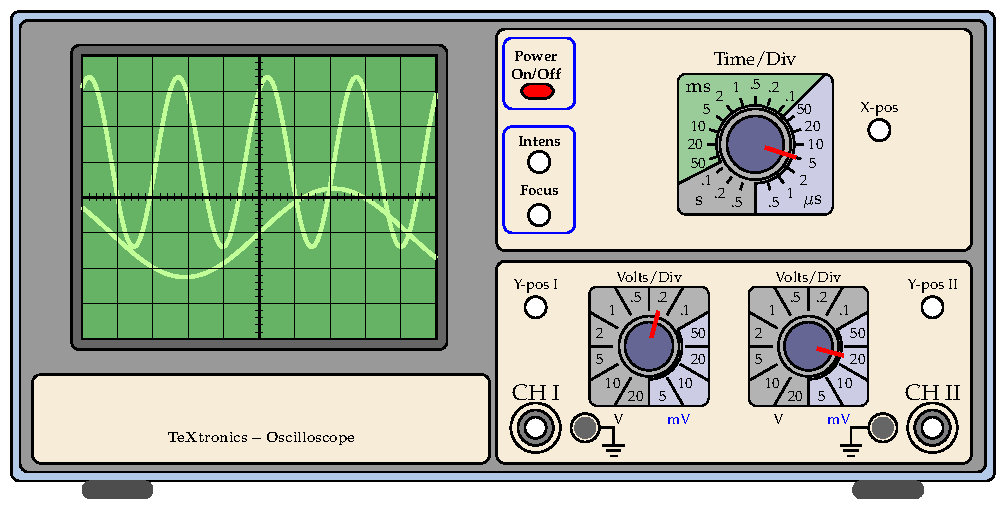
\includegraphics[height=190pt]{oscilloscope.pdf}
\end{center}

an oscilloscope is basically an electron deflection tube that uses a beam of electrons to trace the input voltage as a function of time.

electron beam is controlled by two sets of parallel plates

horizontal plates control how fast beam moves across screen, giving a horizontal time axis

a.c. voltage is applied across vertical plates, causing beam to bend upwards or downwards

when beam hits fluorescent screen, entire trace of the beam can be seen across the screen

\cmt to take readings from oscilloscope, remember it displays a voltage against time graph

\begin{compactenum}
	\item[-] \keypoint{voltage gain}, or \keypoint{Y-gain}, tells the number of volts per vertical division
	
	\item[-] \keypoint{time base} gives the time unit per horizontal division
\end{compactenum}




\example{An oscilloscope displays an a.c. voltage signal as shown.}\label{ex-readcro}

\begin{marginfigure}
\centering
\begin{tikzpicture}[scale=0.8]
\draw[style=help lines,step=1] (0,-3) grid (7,2);
\draw [ultra thick,color=blue,domain=0:7,samples=40,smooth,variable=\x] plot (\x,{2*sin(((\x- 1.7)*2*pi/3 ) r) -0.5 });
\end{tikzpicture}
\end{marginfigure}

suppose the time base setting is $10$ ms/div, and the voltage gain is $5$ V/div.
 
4 vertical divisions from highest to lowest, so

\eqskip peak voltage: $V_0= \frac{1}{2} \times 4 \times 5 = 10 \text{ V}$

3 horizontal divisions between peak to peak, so

\eqskip period: $T = 3 \times 10 = 30 \text{ ms}$
	
\eqskip frequency $f = \frac{1}{T} = \frac{1}{30\times10^{-3}} \approx 33.3 \text{ Hz} $ 



\question{In Example \ref{ex-readcro}, if the time-base setting is 5 ms/div and the voltage gain is 2 V/div, write down an equation that represents this alternating voltage.}



\subsection{power supply systems}

\subsection{high-voltage transmission}

electricity is sent from power stations to consumers around the country

for long-distance transmission, we need minimise energy losses 

power dissipated due to resistance in cables is $I^2 R$, should transmit at low currents

since output power of a power station is fixed, low current means high voltage

so transmission at high voltages minimises energy loss in power grids

but for reasons of safety and efficiency, desirable to have low voltages at both generating end (power station) and receiving end (home or factory)

this requires converting a.c. into higher or lower voltages $\ra$ need for \emph{transformers}

\begin{figure}[ht]
	\centering
	\begin{tikzpicture}[force/.style={align=center,execute at begin node=\setlength{\baselineskip}{1.2em},draw,thick,rounded corners,inner sep=.25cm}]
	
	\node [force] (powerstation) at (0,0) {power\\station};
	\node [force] (step-up) at (3.6,0) {step-up\\transformer};
	\node [force] (step-down) at (8.6,0) {step-down\\transformer};
	\node [force] (home) at (12.6,0) {home or\\factory};
	
	\draw[thick] (powerstation) to node[midway,above]{\footnotesize $5\sim30$ kV} (step-up) to node[midway,above]{\footnotesize $100\sim750$ kV} node[midway,below]{\footnotesize power grid} (step-down) to node[midway,above]{\footnotesize $100\sim250$ V} (home);
	
	\end{tikzpicture}
\end{figure}

\subsection{transformers}  \label{subsection:transformers}

\keypoint{transformer}\index{transformer} is a device that can change values of voltage for an alternating current

transformers are an important part of the national power grid

transformers are essential for transmission, distribution, and utilization of electrical energy


\begin{figure}[ht]
	\centering
\begin{tikzpicture}[scale=1.35]
\draw[thick,rounded corners,fill=gray!15] (-2,-2.2) rectangle (2,2.2);
\draw[thick,rounded corners,fill=white] (-1.2,-1.4) rectangle (1.2,1.4);
\draw[very thick] (-3.2,1) -- (-1.2,1) (1.2,1) -- (3.2,1);
\draw[very thick] (-3.2,-1) -- (-1.2,-1) (1.2,-1) -- (3.2,-1);
\foreach \x in {0.95,0.85,...,-0.95} \draw[very thick] (-2,\x) -- ++ (0.8,-0.05);
\foreach \x in {0.95,0.75,...,-0.95} \draw[very thick] (1.2,\x) -- ++ (0.8,-0.05);
\draw[very thick,<->] (-2.8,1) node[above]{input} -- (-2.8,0) node[left]{$V_p$} --(-2.8,-1);
\draw[very thick,<->] (2.8,1) node[above]{output} -- (2.8,0) node[right]{$V_s$} --(2.8,-1);
\draw[thick] (-1.6,-1.1) -- (-2.5,-2.4) node[below,twoline]{primary\\coil};
\draw[thick] (1.6,-1.1) -- (2.5,-2.4) node[below,twoline]{secondary\\coil};
\draw[thick] (0,1.8) -- (1,2.7) node[right]{iron core};
\end{tikzpicture}

structure of a typical transformer
\end{figure}

\cmt principle of transformers

a.c. flowing in \keypoint{primary coil} (input) produces a changing magnetic field, i.e. a changing flux

this flux is linked with \keypoint{secondary coil} through iron core

an a.c. voltage with same frequency is then induced in secondary coil (output)

\cmt \keypoint{turns-ratio equation} for a transformer

assume no loss in magnetic flux, i.e., all field inside transformer's iron core

from Faraday's law: $V_p = N_p \frac{\dd \phi}{\dd t}$, $V_s = N_s \frac{\dd \phi}{\dd t}$, where $N_p$, $N_s$ are number of turns of coils

\eqyskip cancel out $\frac{\dd \phi}{\dd t}$, we find: $\tcbhighmath{ \frac{V_s}{V_p} = \frac{N_s}{N_p} }$



\xskip 
if $N_p < N_s$, output voltage is increased $\,\rightarrow\,$ \emph{step-up transformers}

if $N_p > N_s$, output voltage is decreased $\,\rightarrow\,$ \emph{step-down transformers}

\cmt if transformer is 100\% efficient, then input power equals output power

for ideal transformers: $\tcbhighmath{I_p V_p  = I_s V_s} $

\cmt in practice, there always exists losses of energy from the transformer

causes of energy loss from the transformer include

\begin{compactitem}
\item[-] heat produced by \emph{eddy currents} induced in iron core

this is reduced by \emph{laminating} the core with insulate layers

\item[-] heat generated in coils due to resistance

can use thick copper wire to minimise resistance

\item[-] leakage of magnetic flux into surroundings

transformer's core is made of a continuous loop of iron to minimise this effect

\end{compactitem}

\example{An ideal transformer has 200 turns on the primary coil and 5000 turns on the secondary	coil. The r.m.s. input voltage to the primary coil is 8.0 V. What is the \emph{peak} voltage across a resistor connected to the secondary coil?}

\begin{soln}\begin{equation*}
\frac{V_{s,0}}{V_{p,0}} = \frac{N_s}{N_p} \RA 
\frac{V_{s,0}}{\sqrt{2}V_{p,\text{rms}}} = \frac{N_s}{N_p} \RA
\frac{V_{s,0}}{8.0\times\sqrt{2}} = \RA
V_{s,0} \approx 2830 \text{ V}   
\end{equation*}
\end{soln}
\question{An ideal transformer has 6000 turns on its primary coil. It converts a mains supply of 220 V r.m.s. to an a.c. voltage with a peak value of 12.0 V. Find the number of turns on the secondary coil.}

\question{If a \emph{steady} d.c. voltage is applied to the input of a simple transformer, what is the output voltage produced?}

\question{State and explain whether the current in the primary coil of a transformer is in \emph{phase} with the voltage induced in the secondary coil.}

\subsection{rectifiers}

some electronic equipments (e.g., your smartphone, laptop, etc.) must work with d.c.

for these appliances require \keypoint{rectification}\index{rectification}, a process that converts an a.c. into a d.c.

rectification uses \emph{diodes}\index{diode}, electronic components that only allow current in one direction

\subsection*{half-wave rectification}\index{rectification!half-wave rectification}


half-wave rectification uses a single diode

\begin{figure}[ht]
	\centering
	\begin{minipage}{0.4\linewidth}
			\centering
			\begin{circuitikz}[xscale=1,yscale=1.1,european resistors]
				\draw (0,0) to[sV,l^=$V_\text{in}$] (0,3) to[Do] (3,3) to[R,l_=$R$] (3,0) -- (0,0);
				\draw (3,3) -- (4.2,3) (3,0) -- (4.2,0);
				\draw[<->] (3.8,0) --++ (0,3) node[right,midway]{$V_\text{out}$};
				\node[right] at (0,2.2) {$X$};
				\node[right] at (0,0.8) {$Y$};
				\node[right] at (3,2.4) {$P$};
				\node[right] at (3,0.6) {$Q$};
			\end{circuitikz}
		\end{minipage}\hfil
	\begin{minipage}{0.54\linewidth}
		\centering
		\begin{tikzpicture}[xscale=0.75,yscale=1.5]
		\draw [thick, ->] (-0.5,0) --(2.7*pi,0) node[below]{$t$};
		\draw [thick, ->] (0,-1.2) --(0,1.2) node[left]{$V$};
		\draw[ultra thick, dotted, gray, domain=0:2.5*pi,smooth,variable=\x] plot (\x,{sin(2*\x r)});
		\foreach \i in {0,1,2}
		\draw [very thick,opacity=0.7,blue,domain=\i*pi:(\i+0.5)*pi,smooth,variable=\x] plot (\x,{sin(2*\x r)});
		\draw [very thick, opacity=0.7,blue] (0.5*pi,0) -- (pi,0) (1.5*pi,0) -- (2*pi,0);
		\draw (6.1,-0.5) --++ (1,-0.2) node[right]{$V_\text{in}$};
		\draw[blue] (2.4*pi,0.7) --++ (0.6,0.2) node[right]{$V_\text{out}$};
		\end{tikzpicture}
		
	\end{minipage}
\end{figure}

when input terminal $X$ is positive, current can flow through diode, terminal $P$ is positive with respect to $Q$ for load resistor $R$ 

when input terminal $Y$ is negative, flow of current is blocked, so zero output voltage on $R$

$V_\text{out}$ across load $R$ is in one direction only, i.e., it becomes a d.c.

but power available from half-wave rectifier is only half of supply power

\subsection*{full-wave rectification}\index{rectification!full-wave rectification}

full-wave rectification requires using a combination of four-diode bridge structure

\begin{figure}[ht]
	\centering
	\begin{circuitikz}[scale=1.2,european resistors]
		\draw (0,-2) -- (-3.2,-2) to[sV,l^=$V_\text{in}$] (-3.2,2) -- (0,2);
		\draw (-2,0) to[Do] (0,2) to[Do] (2,0);
		\draw (-2,0) to[Do] (0,-2) to[Do] (2,0);
		\foreach \r in {1.35} \draw (-\r,\r) node{$A$} (\r,\r) node{$B$} (\r,-\r) node{$C$} (-\r,-\r) node{$D$};
		\draw[fill] (0,2) circle (0.05) (0,-2) circle (0.05) (2,0) circle (0.05) (-2,0) circle (0.05);
		\draw (-2,0) -- (-2,-3) -- (3,-3) to[R,l^=$R$] (3,0) -- (2,0);
		\draw (3,-3) -- (4.2,-3) (3,0) -- (4.2,0);
		\draw[<->] (3.8,0) --++ (0,-3) node[right,midway]{$V_\text{out}$};
		\node[right] at (-3.2,0.7) {$X$};
		\node[right] at (-3.2,-0.7) {$Y$};
		\node[right] at (3,-0.6) {$P$};
		\node[right] at (3,-2.4) {$Q$};
	\end{circuitikz}
\end{figure}

when input terminal $X$ is positive, current flow: $X \to B \to R \to D \to Y $

when input terminal $Y$ is positive, current flow: $Y \to C \to R \to A \to X $

either case, resulting output current in load resistor $R$ always flows in same direction

terminal $P$ is always positive with respect to $Q$ for $R$ no matter what polarity for $V_\text{in}$

output voltage across $R$ is now full-wave rectified


\begin{figure}[ht]
\centering
\begin{tikzpicture}[xscale=1,yscale=1.6]
\draw [thick, ->] (-0.5,0) --(2.7*pi,0) node[below]{$t$};
\draw [thick, ->] (0,-1.2) --(0,1.2) node[left]{$V$};
\draw[ultra thick, dotted, gray, domain=0:2.5*pi,smooth,variable=\x] plot (\x,{sin(2*\x r)});
\foreach \i in {0,1,2}
\draw [very thick, blue, opacity=0.7, domain=\i*pi:(\i+0.5)*pi, smooth, variable=\x] plot (\x,{sin(2*\x r)});
\foreach \i in {0.5,1.5}
\draw [very thick, blue, opacity=0.7, domain=\i*pi:(\i+0.5)*pi, smooth, variable=\x] plot (\x,{-sin(2*\x r)});
\draw (6.1,-0.5) --++ (1,-0.2) node[right]{$V_\text{in}$};
\draw[blue] (2.4*pi,0.7) --++ (0.6,0.2) node[right]{$V_\text{out}$};
\end{tikzpicture}
\end{figure}

\question{If we want to have terminal $Q$ to be positive with respect to $P$ for load resistor $R$, how should we rebuild the bridge rectifier with the same four diodes?}


\subsection{smoothing}

note that d.c. resulting from rectification still varies with time

to produce steady d.c. from fluctuating d.c., a process called \keypoint{smoothing}\index{smoothing} is carried out

smoothing uses \emph{capacitors}\index{capacitor}, which are connected in \emph{parallel} with the load resistor (see figure)

\begin{figure}[ht]
	\centering
	\begin{circuitikz}[scale=0.95,european resistors]
		\draw (0,-2) -- (-3,-2) to[sV,l^=$V_\text{in}$] (-3,2) -- (0,2);
		\draw (-2,0) to[Do] (0,2) to[Do] (2,0);
		\draw (-2,0) to[Do] (0,-2) to[Do] (2,0);
		\draw[fill] (0,2) circle (0.08) (0,-2) circle (0.08) (2,0) circle (0.08) (-2,0) circle (0.08);
		\draw (-2,0) -- (-2,-3) -- (3,-3) to[R,l^=$R$] (3,0) -- (2,0);
		\draw (3,-3) -- (4.5,-3) to[C,l^=$C$] (4.5,0) -- (3,0);
		\draw (4.5,-3) -- (6,-3) (4.5,0) -- (6,0);
		\draw[<->] (5.5,-3) -- (5.5,-1.5) node[right]{$V_\text{out}$} -- (5.5,0);
	\end{circuitikz}
\end{figure}

capacitor can store electrical energy as voltage output from rectifier rises

as voltage from rectifier drops, capacitor slowly discharges and feeds energy to the load 

output voltage $V_\text{out}$ across load will have less ripples over the cycles

less fluctuation in $V_\text{out}$ so we say $V_\text{out}$ is now smoothed

\begin{figure}[ht]
	\centering
\begin{tikzpicture}[xscale=1.35,yscale=2.7]
\draw [thick, ->] (-0.2,0) --(2.2*pi,0) node[below]{$t$};
\draw [thick, ->] (0,-0.2) --(0,1.2) node[left]{$V$};
\foreach \i in {0,1} {
\draw [very thick,blue,domain=(\i+0.16)*pi:(\i+0.25)*pi,smooth,variable=\x] plot (\x,{sin(2*\x r)});
\draw [thick, dashed,gray,domain=\i*pi:(\i+0.5)*pi,smooth,variable=\x] plot (\x,{sin(2*\x r)});
}
\foreach \i in {0.5,1.5} {
\draw [very thick,blue,domain=(\i+0.16)*pi:(\i+0.25)*pi,smooth,variable=\x] plot (\x,{-sin(2*\x r)});
\draw [thick, dashed,gray,domain=\i*pi:(\i+0.5)*pi,smooth,variable=\x] plot (\x,{-sin(2*\x r)});
}

\foreach \i in {0,0.5,1,1.5} 
\draw [very thick,blue] (\i*pi+0.25*pi,1) [out=-10,in=175] to (\i*pi+0.66*pi,0.844);

\draw [very thick,blue] (0,0.9) [out=-7,in=175] to (0.16*pi,0.844);
\draw (2*pi-0.1,0.4) --++ (0.8,0.1) node[right,twoline]{$V_\text{out}$ without\\smoothing};
\draw[blue] (2*pi,0.95) --++ (0.6,0.2) node[right,twoline]{$V_\text{out}$ after\\smoothing};
\end{tikzpicture}
\end{figure}

\cmt effect of smoothing is controlled by choice of load resistor $R$ and smoothing capacitor $C$

rate of charging and discharging depend on \emph{time constant} $RC$ (see \S\ref{sec:charging-capacitors})

greater $RC$, smoothing capacitor discharges more slowly, giving less ripples

a larger capacitor for a fixed resistor usually gives better smoothing effect

but if $RC$ is too large, charging would become very slow, capacitor might not be completely charged after each cycle, this could also result into undesirable effects

\question{If a second capacitor is added in \emph{series} with the first smoothing capacitor, use sketches to show the changes you would expect for the output voltage.}
% \chapter{Quantum Physics Basics}

In this chapter, we will study the laws of nature at very small scales.

We start by reviewing classical concepts like particles or waves, and then see how they break down when being applied to the microscopic world. For those observations that could not be explained with classical physics, we need \emph{quantum physics}. The theory of quantum physics is very deep and profound, so surely way beyond the scope of our course. What we will study in this A-Level course are merely four tips of an enormous iceberg, namely

\begin{compactenum}
	\item[-] photon theory / photoelectric effect
	
	\item[-] matter waves / electron diffraction
	
	\item[-] electron energy levels / atomic spectra
	
	\item[-] band theory / electrical conductivity of solids
\end{compactenum}

\subsection{classical theories}

in classical physics, both particle models and the wave models have been very useful

though both being successful, the two model are distinct in many aspects

to understand a phenomenon, we take either the particle picture or the wave picture

it seems that there is no way particle models would reconcile with wave models, or is it not?

\subsection{particle models}

in particle model, any system is considered to consist of particles governed by \emph{Newtonian mechanics}, physical properties of this system are predicted by studying behaviour of particles

\cmt areas of science where particle models are used to interpret and make predictions include:

\begin{compactenum}
	\item[-] \emph{electricity}: electric current formed by motion of charge carriers
	
	\item[-] \emph{ideal gas}: pressure caused by collisions of gas molecules
	
	\item[-] \emph{solid}: elasticity due to interaction between solid atoms
	
	\item[-] \emph{radioactivity}: decay interpreted as the emission of $\alpha$-/$\beta$-particles from the nucleus
	
	\item[-] \emph{chemistry}: chemical reactions due to exchange of electrons between atoms and molecules
	
	\item[-] $\cdots$
\end{compactenum}

\subsection{wave models}

in the wave picture, energy is transferred via the vibration of medium or force fields

\cmt phenomena that can be explained in terms of wave models include:

\begin{compactenum}
	\item[-] \emph{water waves}: variation in the vertical displacement of water surface
	
	\item[-] \emph{propagation of sound}: variation in the pressure and density of medium
	
	\item[-] \emph{light}: variation of electric and magnetic fields
	
	\item[-] $\cdots$
\end{compactenum}

\cmt a key feature that makes waves distinct from particles is that waves can \emph{superpose}

when two or more waves meet, they add up or cancel out to give a resultant wave

this gives rise to the characteristic properties of waves:

\begin{compactenum}
	\item[-] \emph{interference}: waves superpose to form a resultant wave of greater or lower amplitude
	
	\item[-] \emph{diffraction}: bending of waves around obstacles, or spreading out of waves through slits
\end{compactenum}



\subsection{history of light}

efforts to understand the nature of light can be traced all the way back to ancient Greeks 

we are not going to examine the ideas of early thinkers well over 3,000 years ago

let's skip a couple of years and jump to the ideas developed since the Scientific Revolution


\cmt particle theory of light (\emph{Issac Newton}, 1671)

key idea: light rays is comprised of a stream of massless particles called \emph{corpuscles}

\begin{compactitem}
	\item[--] explains straight-line propagation
	
	\item[--] explains reflection and refraction
	
	\item[--] explains colours of light seen in dispersion in prism (corpuscles have different colours)
\end{compactitem}

the problems with the particle model include:

\begin{compactitem}
	\item[--] does not agree with observations on refraction
	
	\item[--] cannot predict the interference and diffraction of light
\end{compactitem}

\cmt wave theory of light (\emph{Christian Huygens}, 1678)

key idea: light is a wave that transfers energy within a medium known as \emph{aether}

\begin{compactitem}
	\item[--] follows laws of reflection and refraction
	
	\item[--] explains colours of light (light have different wavelengths)
	
	\item[--] explains interference (Thomas Young's double slit experiment)
	
	\item[--] explains diffraction (Poisson spot experiment)
\end{compactitem}

only problem is that aether, the medium in which light lives, was not experimentally found

\cmt electromagnetic theory (\emph{James Maxwell}, 1865)

key idea: light is an \emph{electromagnetic wave}
\footnote{\emph{Maxwell's equations} fully describe the behaviour of electric and magnetic fields. Based on the four equations that Maxwell established, he found the vibration of electric and magnetic field can propagate in space as a classical wave. The speed of electromagnetic wave is given by
	
	{
		
		\centering
		
		$c=\frac{1}{\sqrt{\epsilon_0\mu_0}}=\frac{1}{\sqrt{8.85\times10^{-12}\times4\pi\times10^{-7}}} = 3.00 \times 10^8 \mps$,
		
	}
	
	\noindent which is the same as speed of light. This gave Maxwell the intuition that light is an electromagnetic wave.}

\begin{compactitem}
	\item[--] electric and magnetic fields travel through space in the form of waves at speed of light
	
	\item[--] propagation of electromagnetic wave does not require medium, hence no need for aether
	
\end{compactitem}

all behaviour of light known at that time could be explained with Maxwell's theory

so scientists were convinced that light travelled through space as an electromagnetic wave


\subsection{photon theory}


\subsection{photoelectric effect}\label{ch-photoelectricity}

electromagnetic radiation incident upon a metal can cause emission of electrons from the metal surface, this is called \keypoint{photoelectric effect}\index{photoelectric effect}, 
\footnote{Photoelectric effect was first observed in 1887 by \emph{Heinrich Hertz}, who found electrodes illuminated with ultraviolet light create electric sparks. In school labs, one can shine ultraviolet radiation from a mercury lamp onto a zinc plate to cause photo-emission.}
emitted electrons are called \keypoint{photoelectrons}

simply put, conduction electrons in metal gain additional energy by absorbing the incoming radiation, if this energy is sufficient for electrons to overcome the electrostatic attraction from the positive metal ions, they break free from the metal surface.

\begin{figure}
	\centering
	\begin{tikzpicture}[scale=1.2]
	\tikzset{photon/.style={thick, decorate, purple, decoration={snake,segment length=0.8cm,amplitude=4pt}}}
	\draw[thick] (-3,-1) -- (-1.5,1) -- (3,1) -- (1.5,-1) -- cycle;
	\foreach \r in {-4,-3.5,-3} \draw[photon,->] (\r,\r+6) --++ (2.7,-2.5);
	\foreach \r in {-0.5,0,0.5} \draw[blue,thick,->] (\r+0.5,-\r) --++ (3,2.5);
	\shade [ball color = green] (0,0) circle (0.1);
	\shade [ball color = green] (-1,0.5) circle (0.1);
	\shade [ball color = green] (0.8,-0.2) circle (0.1);
	\shade [ball color = green] (0.9,0.7) circle (0.1);
	\shade [ball color = green] (1,-0.7) circle (0.1);
	\shade [ball color = green] (-0.5,-0.4) circle (0.1);
	\shade [ball color = green] (-1.9,-0.6) circle (0.1);
	\draw (-1,-0.8) --++ (-1.2,-0.8) node[left]{metal plate};
	\node[twoline] at (-1.2,2.6) {electromagnetic\\radiation};
	\node[twoline] at (1.5,2.7) {electrons\\released};
	\end{tikzpicture}
\end{figure}


\cmt some detailed experimental observations on the photoelectric effect are:

\begin{compactitem}
	\item[--] there exists a minimum \keypoint{threshold frequency}\index{photoelectric effect!threshold frequency} $f_0$ for incident radiation
	
	when $f<f_0$, no electrons released from metal surface
	
	\item[--] emission of electrons is immediate when radiation is incident as long as $f>f_0$
	
	even low-intensity light is effective
	
	\item[--] increasing intensity has no effect on energies of electrons
	
	\item[--] increasing intensity of incident light causes number of photoelectrons emitted to increase
	
	\item[--] increasing radiation frequency increases electron energies
\end{compactitem}

\cmt wave theory of light fails to explain any of these properties, according to wave model:

\begin{compactitem}
	
	\item[--] electrons could gradually build up energies by absorbing wave energy over time
	
	so radiation at any frequency should all work 
	
	
	\item[--] need very intense light to have immediate effect
	
	\item[--] greater intensity mean higher energy, electrons released should have greater K.E.
	
	\item[--] varying frequency of radiation should have no effect on energy of electrons released
\end{compactitem}

photoelectric effect sees the breakdown of the wave model, some new ideas are needed!

\newpage
\section{The Photo-electric Effect}
When electromagnetic radiation of high enough frequency falls on a metal surface, electrons are emitted from the surface.
For most metals, ultraviolet is needed. For some (including sodium, potassium, caesium), light towards the violet end of the spectrum) will release electrons.

 
\subsection{Demonstrating the Photo-electric Effect}

Either using a zinc plate with a gold leaf electroscope (or a coulombmeter)
\begin{figure*}
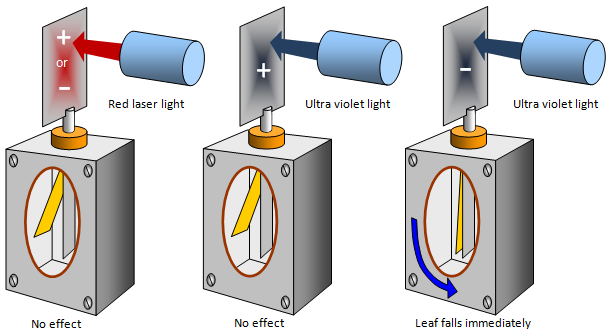
\includegraphics[]{photoelec.png}
\caption{Photoelectric effect demonstrated with electroscope}
\end{figure*}
\begin{itemize}
\item Clean a zinc plate with fine emery paper or steel wool.
\item Attach the plate to the top disc on a gold leaf electroscope, so there is good electrical contact.
\item Charge the zinc plate and inner assembly of the electroscope negatively, e.g. by rubbing the zinc plate with a polythene rod which has been rubbed with wool or fur. The leaf should now be raised, because the leaf and the back plate are both charged negatively and repel each other. The leaf should temporarily rise further if the charged polythene rod is brought near the zinc plate.
\item Place an ultraviolet lamp near the zinc plate. Switch it on. The leaf should be seen to fall. [Safety note: Don't look at the ultraviolet lamp (when it's turned on!)] Clearly the plate (and inner assembly of electroscope) is losing charge.
\item Repeat the procedure, but charging the zinc plate and inner assembly of the electroscope positively, e.g. by rubbing the plate with a charged perspex rod. This time the ultraviolet does not affect the leaf. Charge is not lost.
     \end{itemize}
The simplest explanation is the correct one\ldots The ultraviolet causes electrons to be emitted from the zinc plate. If the plate is charged positively, the electrons are attracted back again. If the plate is charged negatively the emitted electrons are repelled and lost from the plate for ever. 

\subsection{Photo-electric Puzzles}
Before 1905, the energy of a beam of light was thought of as distributed uniformly across broad wavefronts. Calculations showed that it should take some time before an electron in a metal surface could absorb enough energy from the light to escape from the surface. Yet emission is observed as soon as the light falls on the surface.
Another puzzle was why, for a given surface, we find that light of frequency below a certain value (the threshold frequency) causes no electron emission at all.
Einstein's theory of the photo-electric effect solves both these problems\ldots

\subsection{Einstein's Photo-electric Equation}
Although the free electrons in a metal have no allegiance to particular atoms, there are forces `bonding' them to the lattice of ions as a whole. In order to escape from the metal an electron has to do work against these forces. Some have to do more work than others, but there is a certain minimum quantity of work to be done, so no electron can escape unless it is given a certain minimum energy.
The work function, $\phi$, of a metal is the minimum energy needed by an electron in order to escape from the surface. 
Einstein's key idea was that any electron which leaves the surface is ejected by the action of a single photon. Photons don't co-operate in the process.
Recall that a photon of light of frequency $f$ has energy $= hf$. 
Suppose that a photon gives its energy $hf$ to an electron, and that the electron is able to escape. The minimum energy used in escaping is $\phi$, so the maximum kinetic energy the escaped electron can have is what's left over of the photon's energy. So we have the simple equation:
\[ E_{Kinetic} =hf - \phi \]


This assumes that the photon energy is greater than (or equal to) the work function; in other words that  $hf>\phi$ or $f=\phi/h$.
If  $f < \phi/h$, the photon energy will be less than the work function so no electrons at all can escape - a simple explanation of the phenomenon of threshold frequency.
 
The threshold frequency, $f_0$, for a metal is the minimum frequency of electromagnetic radiation needed to produce electron emission from the surface.
From the argument just given, 
\[f_{0} =  \phi/ h.\]
This relationship can also be deduced from Einstein's equation; At the threshold frequency even the most energetic electron will only just manage to escape, so $KE_{max} =  0$, and therefore     $f0 = \phi/h$.
Provided that the light is above the threshold frequency, as soon as it falls on the metal surface electrons will start to be emitted, as emission results from individual photon `hits', and is not a cumulative process as supposed before Einstein.

\subsection{Experimental test of Einstein's Equation}

We use the arrangement with the vacuum photocell shown below  for demonstrating the photoelectric effect.

\begin{figure}
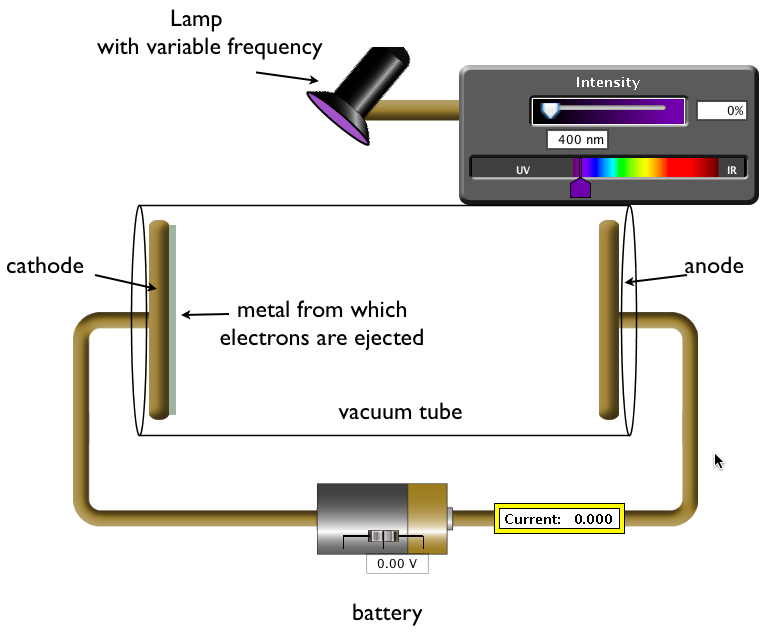
\includegraphics[]{vaccell.png}
\caption{Photoelectric effect with vacuum cell. Note: Picture comes from the fantastic simulation at Phet.}
\end{figure}

\begin{itemize}
\item Use white light with a coloured filter, or a light emitting diode, to illuminate the metal surface with approximately monochromatic light. [Its wavelength can be found using a diffraction grating, hence its frequency, using $f = c / \lambda$ .]
\item Increase the p.d. between the collecting electrode and the metal surface until the current drops to zero. 
At this point the p.d. is called the stopping voltage, $V_{stop}$, because it stops all emitted electrons, even those with the most K.E., from reaching the collector electrode.

\item The maximum K.E. of the emitted electrons is simply given by \sidenote{How do we justify this? Because of the applied voltage, emitted electrons are subject to repulsion by the positive collector electrode and attraction by the emitting surface, hence to a resultant force towards the emitting surface. The electrons therefore get slower and slower as they cross the gap. When the stopping voltage is applied, even the most energetic of emitted electrons have no K.E. left when they have made it across the gap. The K.E. lost is equal to the P.E. gained for these electrons. That's what the equation states.
It is just like finding the K.E. of a ball thrown upwards in the Earth's gravitational field by measuring the its maximum height, and using the energy conservation equation  K.E. lost = mgh}

\[ E_{k} = V_{Stop} \times 1.6 \times 10^{-19} \]


\item Repeat the process using two or three more frequencies of light.
\item Plot a graph of $KE_{max}$ against frequency, $f$. If Einstein's equation is correct it should have a positive slope equal to $h$ and a negative intercept, equal to $ \phi $. We can see this by comparing Einstein's equation with $y = mx + c$.
\begin{align*}
E &= &hf &-& \phi \\
y &= &mx& + &c
\end{align*}
\end{itemize}

A sample graph is presented below.

\begin{figure}
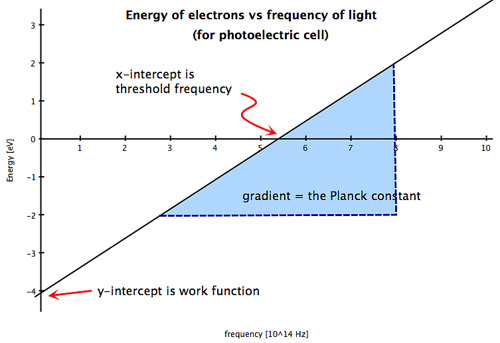
\includegraphics[scale=.6]{photograp.jpg}
\caption{A graph of Frequency vs Kinetic energy}
\end{figure}

It is useful practice to find from the graph:
\begin{itemize}
\item a value of Planck's constant,
\item the threshold frequency for the metal,
\item the threshold wavelength for the metal
\item the work function for the metal
\end{itemize} \sidenote{In practice it is difficult to obtain a good value for h using a commercially available vacuum photocell. Slight impurities on the metal surface (e.g. a thin oxide film), and unwanted electron emission from the collector electrode, both affect the stopping voltage. The first convincing verification of Einstein's photo-electric equation, leading to an accurate value of the Planck constant was completed in 1916 by R.A. Millikan, working in the United States. The secret of his success was a remotely operated knife working in the vacuum to skim off surface layers from the caesium surface as they became contaminated.}
 
\subsection{Effect of changing the Light Intensity}
If we bring a monochromatic light source towards a surface we increase the light energy falling on the surface, per $m^2$, per $s$. We are said to be increasing the intensity of the light. Clearly we can apply the same idea to ultraviolet or any other electromagnetic radiation. We find that:
\begin{enumerate}
\item For light or ultraviolet of a given frequency, changing the intensity has no effect on the maximum K.E. of the emitted electrons. This is exactly what Einstein's theory predicts. The energy given to individual electrons comes from individual photons, and a photon's energy, $hf$, depends only on the frequency (or, equivalently, the wavelength) of the radiation. It doesn't, then, depend on its intensity (provided we don't change the frequency).

\item For light or ultraviolet of a given frequency, increasing the intensity increases the number of electrons emitted per second.
\end{enumerate}
Again, this is just what we'd expect from Einstein's theory. Increasing the intensity means increasing the number of photons arriving at the surface, per m2, per s.  Naturally this means that more electrons will be emitted. \sidenote{Each identical photon has the same probability of emitting an electron.} 
	We can show the effect with the same vacuum photocell arrangement used for demonstrating the photoelectric effect. Note that the polarity of the power supply is arranged to encourage electrons to cross the gap.
    \begin{itemize}
    \item Use a monochromatic light source to illuminate the caesium surface.
\item Check that increasing the p.d. does not affect the current, I. This means that all the electrons emitted per second are being collected.
\item Bring the light source closer and observe the effect on I.
\item I is the charge flowing per second, so the number of electrons emitted per second is I/e in which e is the charge on each electron.
 \end{itemize}





\subsection{photon theory}

photoelectric effect was explained by \emph{Albert Einstein} in 1905
\footnote{Albert Einstein was awarded the Nobel Prize in physics in 1921 for `his discovery of the law of the photoelectric effect'. This discovery led to the quantum revolution of modern physics.}

Einstein's revolutionary idea: when radiation delivers energy to matter, the transfer of energy is not continuous but carried in \emph{discrete} packets, called \emph{photons}

\begin{ilight}
	a \keypoint{photon}\index{photon} is a packet (\emph{quanta}) of electromagnetic energy
\end{ilight}

\cmt energy of one photon is given by: \begin{empheq}[box=\tcbhighmath]{equation*}{E=hf}\end{empheq}, where $h=6.63\times10^{-34} \text{ J s}$ is the \keypoint{Planck constant}\index{Planck constant}

since $E \propto f$, higher/lower radiation frequency means greater/smaller photon energies

\cmt wave equation $c=\lambda f$ relates frequency $f$ of an electromagnetic wave to its wavelength $\lambda$

so energy of one photon is also given by: \begin{empheq}[box=\tcbhighmath]{equation*}{E=\frac{hc}{\lambda}}\end{empheq}

since $E \propto \frac{1}{\lambda}$, longer/shorter wavelength means lower/greater photon energies

\cmt the equation $E=hf$, or $E=\frac{hc}{\lambda}$,  relates a particle property with a wave property

$E$ is the energy of one photon, treated like a single particle

but $f$ and $\lambda$ are both introduced to describe a wave, not a particle

\cmt intensity of a beam of radiation is: $I = \frac{P}{A}$

total energy incident on a given area per unit time determines the radiation intensity

so intensity depends on the product of the number of photons arriving per unit time and energy of each photon: $ \tcbhighmath{I \propto nhf}$, or more precisely, \begin{empheq}[box=\tcbhighmath]{equation*}I = \frac{nhf}{A}\end{empheq}

\cmt when considering energy of a photon, \keypoint{electronvolt} is a useful energy unit

one electronvolt (1 eV) is work needed to make an electron travel through a p.d. of 1 V

conversion between electronvolt and joule is: \begin{empheq}[box=\tcbhighmath]{equation*}{1 \text{ eV} = 1.60\times10^{-19} \text{ J}}\end{empheq}

\example{A laser emits red light of 650 nm at a power rating of 2.0 mW. (a) What is the energy carried by one photon? (b) How many photons are emitted per second?}\label{ex-redlaser}

\begin{soln}
    
energy of one photon: $E = \frac{hc}{\lambda} = \frac{6.63\times10^{-34}\times3.0\times10^8}{650 \times10^{-9}} \approx 3.06\times10^{-19} \text{ J}$

\eqyskip number of photons: $N = \frac{\text{total energy output from laser}}{\text{energy of one photon}} = \frac{2.0\times10^{-3}}{3.06\times10^{-19}} \approx 6.54\times10^{15}$ \end{soln}

\question{Calculate the energy, in eV, of a photon of light of wavelength 440 nm.}

\question{If the light source in Example \ref{ex-redlaser} is replaced by a green laser with the same power output, how does the number of emitted photons per unit time change?}




\subsection{photoelectric effect explained}

from the viewpoint of photon theory, photoelectric effect can be explained easily

to release an electron from metal, it requires a minimum energy $\Phi$, called the \keypoint{work function}\index{photoelectric effect!work function}, for the electron to overcome attraction due to metal ions to escape from metal surface

as radiation shines upon metal, photon energies are absorbed by electrons

since photon energies are \emph{discrete}, or \emph{quantised}, the absorption is sort of all or nothing

if photon energy is greater than $\Phi$, electrons break free from metal

excess energy, if any, would become kinetic energy of the free electron

this is summarised in \keypoint{Einstein's photoelectric equation}\index{photoelectric effect!photoelectric equation}: 
\begin{empheq}[box=\tcbhighmath]{equation*}{hf = \Phi + E_{k,\tmax}}\end{empheq}

\cmt note that we are talking about \emph{maximum} K.E. of emitted electrons

electron emitted from the \emph{surface} would have greatest K.E.

for electrons to be released from \emph{below} the surface, they require more energy than work function, so less K.E. than maximum value

\cmt at critical condition, incoming photon has just enough energy to release electron

so at threshold frequency\index{photoelectric effect!threshold frequency} $f_0$, photon energy equals work function: \begin{empheq}[box=\tcbhighmath]{equation*}{hf_0 = \Phi}\end{empheq}

\cmt experimental observations mentioned in \S\ref{ch-photoelectricity} can now be understood

\begin{compactitem}
	
	\item[--] below threshold frequency $f_0$, not enough photon energy available to electron to overcome work function, so no effect for $f<f_0$
	
	\item[--] interaction between photon and electron is \emph{one-to-one}, so no time delay
	
	\item[--] greater radiation intensity means more photons per unit time, so more electrons released
	
	\item[--] greater frequency means higher photon energy, so greater K.E. for emitted electron
	
\end{compactitem}


\example{Given that work function energy of gold is 4.9 eV. Find the longest wavelength of electromagnetic wave that could release electrons from gold.}

\begin{soln}
    
 threshold frequency: $f_0 = \frac{\Phi}{h} = \frac{4.9\times1.60\times10^{-19}}{6.63\times10^{-34}} \approx 1.18\times10^{18} \text{ Hz}$

threshold wavelength: $\lambda_0 = \frac{c}{f_0} = \frac{3.00\times10^8}{1.18\times10^{15}} \approx 2.54\times10^{-7} \text{ m} \,$ (ultraviolet light) \end{soln}

\question{Sodium has a work function of $3.8\times 10^{-19} \text{ J}$. (a) Find the threshold frequecy for sodium. (b) If a light of 500 nm is incident on sodium, determine whether electrons can be emitted from the surface.}

\question{When electromagnetic radiation of wavelength 1200 nm is incident on a metal surface, the maximum kinetic energy of the electrons released is found to be $5.4\times10^{-20} \text{ J}$. What is the work function of this metal?}

\question{When a beam of light of a particular frequency and intensity is shone onto a metal surface, electrons are released. If another beam of light of same intensity but higher frequency is used, what is the effect on the rate of emission of electrons from this surface?}

\subsection*{measurement of the Planck constant and work function energy}

when radiation with different frequencies is incident onto a metal, we measure maximum K.E. of the electrons emitted from the surface, a set of readings $(f, E_{k,\tmax})$ can be found

note that the photoelectric equation can be rearranged as: $ E_{k,\tmax} = hf - \Phi$

\begin{marginfigure}
	\vspace*{-12pt}
	\centering
	\begin{tikzpicture}[scale=1.2]
	\draw[thick,->] (0,-1.6) -- (0,2.4) node[left]{$E_{k,\tmax}$};
	\draw[thick,->] (0,0) -- (4,0) node[below]{$f$};
	\draw[thick,blue, dashed] (0,-1.2) -- ++(1.6,1.6);
	\draw[thick,blue] (1.6,.4) -- ++(1.8,1.8);	
	\node[left] at (0,-1.2) {$-\Phi$};
	\node[left] at (0,0) {$0$};
	\node[below right] at (1.2,0) {$f_0$};
	\end{tikzpicture}
	\vspace*{-12pt}
\end{marginfigure}

if we plot a graph of $ E_{k,\tmax} $ against $f$, data points shall fall on a straight line

information about the Planck constant $h$, threshold frequency $f_0$, work function $\Phi$ can all be computed with the best-fit line

\begin{compactitem}
	\item[--] $\text{gradient} = h$
	
	\item[--] $y\text{-intercept} = -\Phi$
	
	\item[--] $x\text{-intercept} = \frac{\Phi}{h} = f_0$	
\end{compactitem}

\question{If a different metal with a greater work function energy is used, describe the change for the line that shows the variation with $f$ of $E_{k,\tmax}$ for this metal.}

\question{Electromagnetic adiation is incident upon a metal plate. The graph shows how maximum kinetic energy $E_k$ of emitted electrons varies with frequency $f$ of the radiation. Use the graph to find (a) the threshold frequency, (b) a value of Planck constant.}
	
\begin{center}
	\begin{tikzpicture}[scale=0.96]
		\draw[->] (0,-4.5) -- (0,5.5) node[above]{$E_k$/10$^{-19}$J};
		\draw[->] (0,0) -- (10.5,0) node[right]{$f$/10$^{14}$Hz};
		\draw[step=1, gray, very thin] (0,-4) grid (10,5);
		\foreach \x in {0,1,...,10} {
			\draw[white,fill] (\x-0.2,-0.42) rectangle (\x+0.2,-0.08);
			\node[below] at (\x,0) {$\x$};
		}
		\foreach \y in {-4,-3,...,5} \node[left] at (0,\y) {$\y$};
		\node[blue] at (5.0,0.5) {$\times$};
		\node[blue] at (5.8,1.0) {$\times$};
		\node[blue] at (6.7,1.6) {$\times$};
		\node[blue] at (7.6,2.2) {$\times$};
		\node[blue] at (8.4,2.8) {$\times$};
		\node[blue] at (9.5,3.4) {$\times$};
	\end{tikzpicture}
\end{center}
	


\subsection{photon momentum}

in photoelectric effect, photons can knock electrons out of a metal, this suggests that photons could have \emph{momentum}, even though they do not have mass

earliest experimental evidence of photon momentum was came from \emph{Arthur Compton} in 1923, who studied the scattering of X-ray photons by electrons in substances\footnote{Arthur Compton was awarded the Nobel Physics Prize in 1929 for the discovery of this scattering effect, now known as \emph{Compton scattering}.}

it can be shown\footnote{This derives from Einstein's theory of \emph{special relativity}, which states that energy and momentum are related by the equation: $E^2 = m_0^2 c^4 + p^2 c^2$. Photons have zero rest mass, i.e., $m_0=0$. This relativistic relation becomes $E=pc$ for photons. Now recall photon energy is given by $E=hf$. Rearrange the terms, we can show: $p = \frac{hf}{c} = \frac{h}{\lambda}$.} that photon momentum is given by: \begin{empheq}[box=\tcbhighmath]{equation*}{p = \frac{h}{\lambda}}\end{empheq}

\cmt photon momentum a \emph{relativistic} momentum, as photons move at speed of light

definition for classical momentum $p=mv$ does not apply for photons

\cmt due to exchange of momentum, electromagnetic wave can exert \emph{radiation pressure}

forces generated by radiation pressure are negligible under everyday circumstances, but they could have noticeable effects on spacecraft in outer space and comet tails

\example{A beam of light has wavelength 600 nm, cross-sectional area $0.16 \text{ cm}^2$ and power 5.0 mW. The beam is normally incident onto a surface and is completely absorbed. Calculate, for a time of 1.0 s, (a) the number of photons incident onto the surface, (b) the change of total momentum of the photons, (c) the light pressure on the surface.}

\begin{soln}
    
 energy of one photon: $E= \frac{hc}{\lambda} = \frac{6.63\times10^{-34} \times 3.0\times10^8}{600\times10^{-9}} \approx 3.32 \times 10^{-19} \text{ J}$ 1.5083


number of photons arriving in 1.0 s: $N = \frac{5.0\times10^{-3} \times 1.0}{3.32 \times 10^{-19}} \approx 1.51\times10^{16}$

momentum for one photon: $p = \frac{h}{\lambda} = \frac{6.63\times10^{-34}}{600\times10^{-9}} \approx 1.11 \times 10^{-27} \text{ kg m s}^{-1}$

change of total momentum: $\Delta P = Np = 1.51\times10^{16} \times 1.11 \times 10^{-27} \approx 1.67 \times 10^{-11} \text{ kg m s}^{-1}$

average force due to these photons: $F = \frac{\Delta P}{\Delta t} = \frac{1.67 \times 10^{-11}}{1.0} \approx 1.67 \times 10^{-11} \text{ N}$

light pressure on surface: $p = \frac{F}{A} = \frac{1.67 \times 10^{-11}}{0.16 \times 10^{-4}} \approx 1.04 \times 10^{-6} \text{ Pa}$ \end{soln}

\question{A laser of power $P$ is incident normally on a spot of area $A$, show that the pressure caused by the beam can be given by: $p = \frac{P}{cA}$.}

\question{When an electron and a positron meet together, they will annihilate and produce two $\gamma$-photons: $^{\phantom{+}0}_{-1}e + ^{\phantom{+}0}_{+1}e \longrightarrow \gamma + \gamma$. Assume the electron and the positron have negligible kinetic energy before the interaction, explain why the two photons produced must move off in opposite directions with equal energies.}

\subsection{wave-particle duality}



\subsection{matter waves}

inspired by photon theory, which shows electromagnetic waves have a particulate nature, \emph{Louis de Broglie} suggested in his 1924 PhD thesis that all matter has a wave-like nature
\footnote{Louis de Broglie was awarded the 1929 Nobel Physics Prize `for his discovery of the wave nature of electrons'. \emph{Schr\"oedinger's equation} and \emph{Bohr's atomic model} was heavily influenced by ideas of de Broglie.}

wave characteristic of a particle can be represented by a wavelength

\begin{ilight}
	\keypoint{de Broglie wavelength}\index{de Broglie wavelength} of a matter particle is given by:\begin{empheq}[box=\tcbhighmath]{equation*}{\lambda = \frac{h}{p}}\end{empheq}, where $p=mv$ is the particle's momentum
\end{ilight}

\example{What is the wavelength of a human of 70 kg walking at around $2.0\mps$?}

\begin{soln}
    $\lambda = \frac{h}{mv} = \frac{6.63\times10^{-34}}{75\times 2} \approx 4.7\times 10^{-36} \text{ m}$

this wavelength is too small compared with any obstacle we encounter in everyday lives

so human bodies do not exhibit noticeable wave behaviour \end{soln} 

\example{An electron is accelerated from rest through a potential difference of 50 V. What is the de Broglie wavelength of this electron?}
\begin{soln}
K.E. of electron equals change in electric P.E., so
$\frac{1}{2}mv^2 = qV \RA v = \sqrt{\frac{2qV}{m}} = \sqrt{\frac{2\times1.60\times 10^{-19} \times 50}{9.11\times10^{-31}}} \approx 4.19\times10^6 \mps$


wavelength of electron: $\lambda = \frac{h}{mv} = \frac{6.63\times10^{-34}}{9.11\times10^{-31}\times 4.19\times10^6} \approx 1.74 \times10^{-10} \text{ m}$

this wavelength is comparable to scale of atomic spacing (also around $10^{-10}\text{ m}$)

so these electron can be \emph{diffracted} by solid crystals\end{soln}

\question{An $\alpha$-particle is moving with a kinetic energy of $2.4\times10^{-15} \text{ J}$. Find its speed, and hence find its de Broglie wavelength.}

\question{If a proton and an electron are accelerated through the same voltage, (a) how would their energy compare? (b) how would their wavelength compare?}

\subsection{electron diffraction}


wave property of electron was confirmed by \emph{Clinton Davisson} and \emph{George Thomson} in 1927

they showed experimentally electrons could be diffracted\index{electron diffraction} by metal crystals
\footnote{The Nobel Prize in Physics 1937 was awarded jointly to Clinton Davisson and George Thomson `for their experimental discovery of the diffraction of electrons by crystals'}

\begin{figure}[htp]
	\centering
	\begin{tikzpicture}[scale=1]
	\draw[gray!40,fill] (-0.5,-1) -- (-0.5,0.5) -- (0.5,1) -- (0.5,-0.5) -- cycle;
	\draw[thick,blue,->] (-3,0) -- (-.5,0);
	\draw[gray!20,fill] (5,-3) -- (5,1.5) -- (7,3) -- (7,-1.5) -- cycle;
	\draw[blue, dashed, fill=blue!50, opacity=0.3] (0,0) -- (6,1.2) [out = 0, in=0] to (6,-1.2) --cycle;
	\draw[blue, dashed, opacity=0.3] (6,1.2) [out = 180, in=180] to (6,-1.2);
	\draw[green,fill] (6,0) ellipse (0.06 and 0.12);
	\draw[green,line width=2pt] (6,0) ellipse (0.2 and 0.4);
	\draw[green,line width=2pt] (6,0) ellipse (0.35 and 0.7);
	\draw[green,line width=1.5pt] (6,0) ellipse (0.55 and 1.1);
	\draw (-0.2,-0.5) --++ (-0.5,-1) node[below,twoline]{thin\\crystal};
	\draw (5.5,-2) --++ (2,-0.6) node[below,twoline] {fluoroscent\\screen};
	\draw (6.3,0.9) --++ (2.5,1.5) node[above,twoline] {diffraction pattern\\formed on screen};
	\node[twoline] at (-1.8,0.5) {electron\\beam};
	\end{tikzpicture}
	
	\caption{electron diffraction experiment}
\end{figure}

\cmt electron diffraction experiment shows that particles do have wave-like properties

if electrons behaved like particles, we would see a round spot of \emph{uniform} distribution

but the actual pattern formed on \emph{fluorescent screen} is a set of \emph{concentric rings}

this is a typical diffraction pattern, hence proves wave properties of electrons

\cmt each metal has a different lattice structure, so each produces a different pattern

this allows investigation of structure of matter (explore arrangements of atoms, structures of complex molecules, structure of atomic nuclei, etc.) using electron diffraction

\cmt since wavelength of an electron is much shorter than visible light

this allows \emph{electron microscope} to have much higher resolving power than optical microscopes

\question{If a higher p.d. is applied to accelerate the electron beam in the electron diffraction experiment, how would the pattern change?}


\subsection{wave-particle duality}

we have seen both particle-like and wave-like behaviour in light and electrons

\begin{center}
	\begin{tabular}{|D{2.5cm}|D{5.5cm}|D{5cm}|}
		\hline
		& electromagnetic radiation & electron \\ \hline
		particle-like & photoelectric effect, & deflection in electric/magnetic \\
		behaviour & radiation 	pressure &  fields, decay, scattering \\  \hline
		wave-like behaviour & interference, diffraction, Doppler
		effect, reflection, refraction & electron diffraction \\ \hline
	\end{tabular}
\end{center}

when light/electron move through space, they behave like a wave

when light/electron interact with each other, they behave like particles

they show a two-sided nature, or a \emph{dual} nature of being both a wave and a particle, described by either particle model or wave model under different circumstances

in fact, all matter (protons, neutrons, atoms, cells, basketballs, human body, earth, etc.) has this universal dual nature, called \keypoint{wave-particle duality}\index{wave-particle duality}

wave-particle duality addresses breakdown of classical concepts like particle or wave

to fully describe the behaviour of microscopic objects, we need \emph{quantum mechanics}
\footnote{Being a central concept of quantum theory, wave-particle duality is deeply embedded into the foundations of quantum physics. In non-relativistic quantum mechanics, all information about a particle is encoded in its \emph{wave function}, whose evolution with time is described by the famous \emph{Schr\"odinger's equation}.}




\subsection{quantisation of electron energy levels}

in a simple atomic model, electrons move around the nucleus in circular orbits

but now we understand electrons have wave properties, as an electron moves in its orbit as a wave, it can superpose with itself

only orbits in which the electron can superpose constructively with itself are preferable

so electrons are only allowed to move in certain orbits in an atom

this means can only take certain values of energy, called \emph{energy levels}



\subsection{hydrogen atom \protect\piste}

theoretical explanation for electron energy levels was developed in 1913 by Danish physicist \emph{Niels Bohr} in his theory of hydrogen atom
\footnote{Niels Bohr was surely one of the greatest physicists of the 20th century. He made foundational contributions to understanding atomic structure and quantum mechanics, for which he received the Nobel Physics Prize in 1922. He was also the founder of the Institute of Theoretical Physics at the University of Copenhagen, which soon became the centre of pioneering researches on quantum theory in the world.}

let's look at the hydrogen atom -- the simplest possible atom in nature

\begin{marginfigure}
	\centering
	\begin{tikzpicture}[scale=0.7]
	\draw[thick,domain=0:360,samples=120] plot (\x:{3+.5*cos(5*\x)});
	\draw[thick,dashed] (0,0) circle (3);
	\shade [ball color = blue] (0,0) circle (0.15) node[below]{\scriptsize proton};
	\shade [ball color = green] (65:3.4096) circle (0.15) node[above right]{\scriptsize electron};
	\end{tikzpicture}
	
	\caption{the hydrogen atom}
\end{marginfigure}

electrostatic attraction by proton provides centripetal force for electron to move in circles



{
	
	\centering
	
	$\frac{e^2}{\ec r^2} = \frac{m_e v^2}{r} \RA v^2 = \frac{e^2}{\ec m_e r}$
	
}

for electron to \emph{constructively} superpose with itself, the perimeter of its orbit must be an integer multiple of its de Broglie wavelength

{
	
	\centering
	
	$2\pi r  = n \lambda \RA 2\pi r = \frac{nh}{m_e v} \RA v = \frac{nh}{2\pi m_e r}$
	
}

\noindent where $n$ is positive integer $1,2,3,\cdots$

compare the two equations, we can eliminate $v$

{
	
	\centering
	
	$\frac{e^2}{\ec m_e r} = \frac{n^2 h^2}{4\pi^2 m_e^2 r^2}$
	
}

we hence find radius of allowed orbits satisfies:

{
	
	\centering
	
	$\boxed{r_n = n^2 a_0} \quad \text{where }\, a_0 = \frac{h^2 \epsilon_0}{\pi m_e e^2} \approx 5.29 \times 10^{-11} \text{ m}$
	
}

\noindent so we see all allowed orbits must have a radius equal to integer multiple of $a_0$

total energy possessed by the electron consist of K.E. and electric P.E.:

{
	
	\centering
	
	$E = E_k + E_p = \frac{1}{2}m_e v^2 - \frac{e^2}{\ec r} = \frac{1}{2}m_e \frac{e^2}{\ec m_e r} - \frac{e^2}{\ec r} \RA E = -\frac{e^2}{8\pi\epsilon_0 r}$
	
}

substitute the allowed orbital radius, we find an expression for electron energy:

{
	
	\centering
	
	\begin{empheq}[box=\tcbhighmath]{equation*}{E_n = -\frac{R_E}{n^2}} \end{empheq} $\text{where }\, R_E = \frac{m_e e^4}{8 h^2 \epsilon_0^2} \approx 2.18\times10^{-18} \text{ J} \approx 13.6 \text{ eV}$
	
}

this shows electron can only have specific energies in the hydrogen atom



\subsection{electron energy levels}

it can be shown that for any atom, electrons can only have certain fixed values of energy

we say energy of electrons in an atom is \emph{discrete}, or \keypoint{quantised}

these allowed values of energies are called \keypoint{energy levels}\index{energy level}\footnote{If you study chemistry, you shall recall this idea of discrete energy levels is related to the concepts of energy shells and sub-shells of atoms.}

\begin{marginfigure}
	\centering
	\begin{tikzpicture}[yscale=0.8,xscale=0.8]
	\foreach \s in {-6,-3.5,-2,-1}
	\draw[thick,blue] (0.5,\s) -- ++ (3.5,0);
	\draw[thick,blue,dashed] (0.5,0) -- ++ (3.5,0);
	\draw[thick,->] (0,-6.5) -- (0,0.6) node[left]{\footnotesize{$E$}};
	\draw(0.1,-6) --++ (-0.2,0) node[left]{$E_1$};
	\draw(0.1,-3.5) --++ (-0.2,0) node[left]{$E_2$};
	\draw(0.1,-2) --++ (-0.2,0) node[left]{$E_3$};
	\draw(0.1,-1) --++ (-0.2,0) node[left]{$E_4$};
	\draw(0.1,0) --++ (-0.2,0) node[left]{$0$};
	\end{tikzpicture}
	
	\caption{electron energy levels of some atom}		
\end{marginfigure}

\cmt \emph{quantisation} means an electron can have only specific values of energy in an atom

no intermediate value between levels is allowed

\cmt the lowest energy level is called the \keypoint{ground state}

any level higher than the ground state is called an \keypoint{excited state}

in our illustration, $E_1$ is the ground state, while $E_2$, $E_3$, $E_4$ are all excited states

\cmt electron energy levels are all \emph{negative}

to pull an electron away from the nucleus, work must be done to overcome electrostatic attraction

an electron at infinity would have greatest P.E., which is defined to be zero 

so orbiting electrons have energies less than zero

an electron that has zero energy would become a \emph{free} electron

\cmt electrons can jump, or \emph{transit}, between energy levels

electron transition is associated with emission or absorption of photon with the right energy



\begin{figure}[ht]
	\centering
	\begin{minipage}{0.48\textwidth}
		\begin{center}
			\begin{tikzpicture}[yscale=0.85,xscale=1]
			\foreach \s in {7,3,1.2,0.5,0.15}
			\draw[thick,blue] (0,-\s) -- ++ (4,0);
			\draw[thick,->] (-1,-7.5) -- (-1,0.2) node[left]{\footnotesize{$E$}};
			\draw[red,thick,->] (0.8,-3) node{$\bullet$} -- (0.8,-7);
			\draw[red,thick,->] (2.1,-1.2) node{$\bullet$} -- (2.1,-7);
			\draw [->, thick, purple, decorate, decoration={snake,post=lineto, post length=2mm}] (0.8,-5.6) --++ (2.4,0) ;
			\draw [->, thick, purple, decorate, decoration={snake,post=lineto, post length=2mm}] (2.1,-4) -- (3.8,-4);
			\node[twoline] at (3.6,-4.8) {photon\\emitted};
			\end{tikzpicture}
		\end{center}
	\end{minipage}\hfil
	\begin{minipage}{0.48\textwidth}
		\begin{center}
			\begin{tikzpicture}[yscale=0.85,xscale=1]
			\foreach \s in {7,3,1.2,0.5,0.15}
			\draw[thick,blue] (0,-\s) -- ++ (4,0);
			\draw[thick,->] (-1,-7.5) -- (-1,0.2) node[left]{\footnotesize{$E$}};
			\draw[red,thick,<-] (1.4,-3) -- (1.4,-7) node{$\bullet$};
			\draw [->, thick, purple, decorate, decoration={snake,post=lineto, post length=2mm}] (0,-5) -- (1.4,-5) ;
			\draw [->, thick, purple, decorate, decoration={snake,post=lineto, post length=2mm}] (0.3,-4) -- (3.6,-4);
			\node[twoline] at (3.5, -4.8){photon not\\absorbed};
			\node[twoline] at (0.5,-5.8){photon\\absorbed};
			\end{tikzpicture}
		\end{center}
	\end{minipage}
	
	\caption{emission and absorption of photons as a result of electron transitions}
\end{figure}


\subsection{atomic spectrum}



passing light through a \emph{prism} or a \emph{diffraction grating}, different wavelengths are separated, a pheonomenon known as \keypoint{dispersion}\index{dispersion}, this produces a \keypoint{spectrum}\index{spectrum} which shows distribution of energy emitted from the source in order of wavelengths

for example, white light consists of a range of wavelengths from around 400 nm to 700 nm, so it gives a \emph{continuous spectrum} with rainbow of colours

\begin{center}
	\pgfdeclareverticalshading{rainbow}{100bp}
	{color(0bp)=(Red); color(25bp)=(Red); color(30bp)=(OrangeRed); color(35bp)=(Orange); color(40bp)=(Gold); color(45bp)=(Yellow); color(50bp)=(GreenYellow); color(55bp)=(LimeGreen); color(60bp)=(Teal); color(65bp)=(DarkBlue); color(70bp)=(Indigo); color(75bp)=(Purple); color(100bp)=(Purple)}
	\begin{tikzpicture}[shading=rainbow]
	\shade[shading angle=90] (0,0) rectangle (12,2);
	\end{tikzpicture}
	
	continuous spectrum of white light
\end{center}

electron transition between different levels causes emission or absorption of photons

this leads to the emission spectrum and absorption spectrum of atoms

\subsection*{emission spectrum}

\emph{hot gases} of an element can release photons, giving an \keypoint{emission spectrum}\index{spectrum!emission spectrum}

this happens when an electron transits from a high energy level to a lower level

energy of the photon emitted is equal to energy difference between the two levels

since electron energy levels are discrete, only specific changes of energies are possible, so only photons with specific energies can be emitted

this means photons emitted only have specific wavelengths, or specific frequencies

so a collection of sharp and bright lines are seen in emission spectrum

\begin{figure*}[ht]
	\centering
	\begin{tikzpicture}
	\draw [fill] (0,0) rectangle (12,2);
	\draw [ultra thick, orange] (11,0) -- (11,2);
	\draw [ultra thick, yellow] (9,0) -- (9,2);
	\draw [ultra thick, green] (3.5,0) -- (3.5,2);
	\draw [ultra thick, blue] (2,0) -- (2,2);
	\end{tikzpicture}
	
	\caption{emission spectrum of the hydrogen atom}
\end{figure*}

\cmt emission spectrum is a \emph{discrete} spectrum, also called a \emph{line} spectrum

\cmt atoms of each element has a unique electron energy level structure

so each element produces a unique emission spectrum, leading to quite a few applications:

\begin{compactitem}
	\item[-] explains the colour of flames when a particular chemical element is present
	
	\item[-] allows the identification of elements in an unknown substance in chemical analysis
	
	\item[-] explains varied colours of electric signs lighted by gas-discharge tubes
\end{compactitem}


\subsection*{absorption spectrum}


pass white light through a \emph{cool gas}, photons with the right energies can be absorbed, giving rise to an \keypoint{absorption line spectrum}\index{spectrum!absorption spectrum}

by absorbing photon, electron can transit from a low energy level to a higher level

energy of the photon absorbed must equal energy difference between the two levels

since electron energy levels are discrete, so only photons with specific energies can be absorbed, while other photons are unaffected as they pass through the gas

wavelengths of these absorbed photons will be missing in the emergent spectrum

so we would observe a set of \emph{dark lines} appearing in a background of continuous spectrum


\begin{figure}[ht]
	\centering
	\begin{tikzpicture}[shading=rainbow]
	\shade[shading angle=90] (0,0) rectangle (12,2);
	\foreach \x  in {1.9,4.4,5.9,7.6,8.2,9.9,11.4}
	\draw [very thick] (\x,0) -- (\x,2);
	\end{tikzpicture}
	\caption{absorption spectrum for some element}
\end{figure}

\cmt absorption spectrum is also a \emph{discrete} spectrum, or a \emph{line} spectrum

\cmt as photons with the right energies are absorbed, they can be re-emitted through \emph{de-excitation}

but these photons are re-emitted in \emph{random} directions

so they would still appear dark compared with those unaffected wavelengths

\cmt absorption spectrum is widely used in many areas

\begin{compactitem}
	\item[-] determine the composition of a particular substance in analytical chemistry
	
	\item[-] determine chemical compositions of stars in astronomical spectroscopy
	
	\item[-] explain colour of chemicals in terms of the complementary colour of photons absorbed  
	
\end{compactitem}


%\vspace*{\baselineskip}

%for either emission or absorption process, energy of photon must match the difference between two electron energy levels: $\boxed{hf = E_\text{high} - E_\text{low}}$

\example{Some electron energy levels of the hydrogen atom is shown. Find the longest and the shortest wavelength produced by electron transitions between the energy levels given.}\label{ex-hydrogen}

\begin{figure}[ht]
	\centering
	\begin{tikzpicture}[scale=0.85]
	\foreach \s in {-6,-2.7,-1.5,-0.7,-0.1}
	\draw[thick,blue] (0.5,\s) -- ++ (3.5,0);
	\draw[thick,->] (0,-6.5) -- (0,0.5) node[left]{\footnotesize{energy}};
	\draw(0.1,-6) --++ (-0.2,0) node[left]{$E_1=-13.6 \text{ eV}$};
	\draw(0.1,-2.7) --++ (-0.2,0) node[left]{$E_2=-3.40 \text{ eV}$};
	\draw(0.1,-1.5) --++ (-0.2,0) node[left]{$E_3=-1.51 \text{ eV}$};
	\draw(0.1,-0.7) --++ (-0.2,0) node[left]{$E_4=-0.85 \text{ eV}$};
	\draw(0.1,-0.1) --++ (-0.2,0) node[left]{$E_5=-0.54 \text{ eV}$};
	\end{tikzpicture}		
	
	\caption{energy levels of the hydrogen atom}
\end{figure}

\begin{soln} energy of photon emitted equals change of electron energy level: $\frac{hc}{\lambda} = \Delta E$, or $\lambda = \frac{hc}{\Delta E}$

transition with least/greatest energy change gives rise to longest/shortest wavelength, so

\eqskip $E_5 \to E_4 \ra \lambda_\tmax = \frac{hc}{E_5-E_4} = \frac{6.63\times10^{-34}\times3.0\times10^8}{(0.85-0.54)\times1.60\times10^{-19}} \approx 4.0\times10^{-6} \text{ m} \quad$ (infra-red)
	
\eqyskip 
	
\eqskip $E_5 \to E_1 \ra  \lambda_\tmin = \frac{hc}{E_5-E_1} = \frac{6.63\times10^{-34}\times3.0\times10^8}{(13.6-0.54)\times1.60\times10^{-19}} \approx 9.5\times10^{-8} \text{ m} \quad$ (ultraviolet) \end{soln}
	

\example{The emission spectrum of the hydrogen atom consists of a number of wavelengths in the visible spectrum. Given that the visible spectrum consists of light of wavelengths within the range from 380 nm to 740 nm, also use data in Example \ref{ex-hydrogen}, find the energies of visible photons that can be produced by transitions between the energy levels shown.}\sidenote{The H$_\alpha$ line is the brightest hydrogen line in the visible range. It plays an important role in astronomy, as it can be used to study a star's surface temperature, the velocity of a distant stellar object, etc.}

\begin{soln} let's first find the range of energies, in eV, for visible photons

\eqskip $E_\tmax = \frac{hc}{\lambda_\tmin} = \frac{6.63\times10^{-34}\times 3.0 \times10^8}{380\times10^{-9}} \approx 5.23\times10^{-19} \text{ J} = \frac{5.23\times10^{-19}}{1.60\times10^{-19}} \text{ eV} \approx 3.27 \text{ eV}$
 $E_\tmin = \frac{hc}{\lambda_\tmax} = \frac{6.63\times10^{-34}\times 3.0 \times10^8}{740\times10^{-9}} \approx 2.69\times10^{-19} \text{ J} = \frac{2.69\times10^{-19}}{1.60\times10^{-19}} \text{ eV} \approx 1.68 \text{ eV}$

we shall find the combinations of electron energy levels such that their difference fall within the range between 1.68 eV and 3.27 eV, by trial and error, we find three possible combinations:

\begin{compactenum}
	\item[(1)] $E_3 \to E_2 \ra 3.40 - 1.51 = 1.89 \text{ eV}$
	
	\item[(2)] $E_4 \to E_2 \ra 3.40 - 0.85 = 2.55 \text{ eV}$
	
	\item[(3)] $E_5 \to E_2 \ra 3.40 - 0.85 = 2.85 \text{ eV}$
\end{compactenum}

these emisssion lines are called H$_\alpha$ (656 nm), H$_\beta$ (486 nm) and H$_\gamma$ (435 nm) lines

they are three of the four the hydrogen emission lines that are visible to human eyes \end{soln}\sidenote{These lines belong to a family of the spectral lines of the hydrogen atom, known as the \emph{Balmer lines}, named after Johann Balmer. Balmer discovered an empirical equation to predict the series in 1885, but the reason why the equation worked was eventually clarified by Neils Bohr with the atomic model which now bears his name. We now understand the Balmer lines correspond to emissions of photons by electrons jumping to the second level from higher energy states.}



\example{A white light is incident on a cloud of cool hydrogen gas. In the emergent spectrum, a dark line is observed at a wavelength of 435 nm. Determine the energy change that gives rise to this dark line.}

\begin{soln}
    
 photon absorbed: $E = \frac{hc}{\lambda} = \frac{6.63\times10^{-34}\times 3.0 \times10^8}{435\times10^{-9}} \approx 4.57\times10^{-19} \text{ J} = \frac{4.57\times10^{-19}}{1.60\times10^{-19}} \text{ eV} \approx 2.86 \text{ eV}$

note that $3.40 - 0.54 = 2.86 \text{ eV}$, so this dark line is due to the electron transition: $E_2 \to E_5$ \end{soln}

\question{If we only consider the electron energy levels given in Example \ref{ex-hydrogen}, how many different wavelengths can be detected in the emission spectrum of the hydrogen atom ?}

\question{Three lines are observed at wavelengths 486 nm , 656 nm, and 1880 nm in the emission spectrum of hydrogen atoms. (a) Calculate the photon energies for these wavelengths. (b) Draw a diagram with \emph{three} labelled energy levels, and show the energy changes for the three wavelengths produced with arrows in your diagram.}

\begin{marginfigure}
	\centering
	\vspace*{-25pt}
	\begin{tikzpicture}[xscale=0.8, yscale=0.65]
	\foreach \s in {-7.6,-5.8,-3.0,-2.4,-1.6} {
	\draw[thick,blue] (0.5,\s) -- ++ (3.5,0);
	\draw(0.1,\s) --++ (-0.2,0) node[left] {\s};
	}
	\draw[thick,->] (0,-8) -- (0,-1) node[above]{\footnotesize{energy/$10^{-19}\text{ J}$}};	
	\end{tikzpicture}		
	
	\caption{energy levels of the helium atom}
	\vspace*{-15pt}
\end{marginfigure}

\question{The relative cool atmosphere of the sun could give rise to dark lines in the spectrum of sunlight.	One particular dark spectral line has a wavelength of 590 nm. By reference to the energy levels of the helium atom, suggest how this dark line provides evidence of the presence of helium in sun's atmosphere. You may draw an arrow to show the possible electron transition that gives rise to this dark line.}



\subsection{band theory}

\subsection{energy bands}

in an isolated atom, electrons have discrete energy levels 

in solids, interaction between neighbouring atoms causes change of energies

original energy levels split into a band with many sub-levels

number of sub-levels in each band equals number of atoms in solid in general

due to very large number of atoms, sub-levels (seem to) form \emph{continuous} \keypoint{energy bands}\index{energy band}

\begin{figure}[htp]
	\centering
	\begin{tikzpicture}[yscale=0.56,xscale=.8]
	\foreach \s in {0,1.5,3.5,7}{
		\draw[thick,blue] (0,-\s) -- ++ (3.6,0);
		\foreach \step in {-0.4,-0.3,...,0.4}	\draw[thick,blue] (6,-\s+\step) -- ++ (3.6,0) ;
		\draw[thick,blue,fill=blue!30] (12,-\s-0.5) rectangle (15.6,-\s+0.5);
	}
	\draw[thick,->] (-.8,-8) -- (-.8,1) node[left]{$E$};
	\node[below,twolinecap] at (1.8,-9) {dicrete energy levels\\in isolated atom};
	\node[below,twolinecap] at (7.8,-9) {split energy sub-levels\\due to interactions};
	\node[below,twolinecap] at (13.8,-9) {energy bands formed\\in many-particle system};
	\end{tikzpicture}
\end{figure}

\begin{marginfigure}
	\vspace*{0pt}
	\centering
	\begin{tikzpicture}[scale=0.8]
	\draw[thick,->] (-1,-0.5) --++ (0,7.2) node[left]{$E$};
	\foreach \s in {0,2.5,5}
	\draw[thick,blue,fill=blue!30] (0,\s) rectangle (4,\s+1);
	\foreach \x in {0.5,1,...,3.5} \foreach \y in {0.3,0.7,2.8,3.2}
	\shade [ball color = green] (\x,\y) circle (0.1); 
	\foreach \x in {0.5,1.5,2.5,3.5} \shade [ball color = green] (\x,5.3) circle (0.1); 
	\node at (4.7,5.5) {CB};
	\node at (4.7,3) {VB};
	\node at (4.7,4.25) {FB};
	\node at (4.7,1.75) {FB};
	\draw[thick,<->] (3,3.5) -- (3,5) node[midway,right]{$E_g$};
	\end{tikzpicture}
	\vspace*{-12pt}
\end{marginfigure}

in solids, electrons fill up from lowest energy bands available (see figure for a rough idea)


\keypoint{forbidden bands}\index{energy band!forbidden band} (FB) represent energies that electrons are not allowed to take



highest fully filled band is called \keypoint{valence band}\index{energy band!valence band} (VB)

next partially filled or empty band is called \keypoint{conduction band}\index{energy band!conduction band} (CB)

separation between valence band and conduction band defines \keypoint{band gap}\index{energy band!band gap} ($E_g$) of material 


\subsection{band theory \& electrical conductivity}\label{band-theory}

electrical conductivity of material can be explained by its band structure

low-energy bands below VB are usually fully filled at all times, all states are occupied, electrons cannot move freely to form electric currents, so we are not interested in low-energy bands

conductivity of material will depend on whether there are free \emph{charge carriers} in CB and VB


\subsection*{metallic conductors}

for typical metals, CB \emph{overlaps} with VB, i.e., there is no band gap

there exist vacant states for conduction electrons to occupy at ease

this means conduction electrons are free to move around to form currents

as temperature rises, there is no significant change in number of free electrons

but \emph{lattice vibration} of atoms increases, electrons become more likely to collide with vibrating atoms, so resistance of metal increases with temperature

\cmt metals are \emph{opaque} to visible light or other low-frequency radiation

width of CB for a typical metal is about $2\sim3 \text{ eV}$

low-energy photons can be absorbed by conduction electrons

visible light, infra-red, microwave therefore cannot pass through metal

\cmt metals are \emph{transparent} to high-frequency radiation such as X-rays

if X-ray photons were absorbed, electrons would take energies in forbidden band

but this is not allowed, so high-frequency photons penetrate through metal

\subsection*{insulators}

\begin{marginfigure}
	\vspace*{-5pt}
	\centering
	\begin{tikzpicture}[scale=0.72]
	\foreach \s in {0,2,7}
	\draw[thick,blue,fill=blue!30] (0,\s) rectangle (4,\s+1);
	\foreach \x in {0.5,1,...,3.5} \foreach \y in {0.3,0.7,2.3,2.7}
	\shade [ball color = green] (\x,\y) circle (0.1); 
	\node at (4.7,7.5) {CB};
	\node at (4.7,2.5) {VB};
	\end{tikzpicture}
	
	band structure of insulator
\end{marginfigure}

examples of insulators include glass, diamond, etc.

in normal conditions, CB of insulator is empty, energy bands up to VB are fully filled, so no movement of electron is possible, material has poor conductivity

insulators also have huge band gap\footnote{To be a little more precise, materials with a band gap $E_g \approx 5$ eV or greater are regarded as insulators.}\footnote{There exist a class of insulators called \emph{Mott insulators} which do not have large band gaps. Their poor conductivity at low temperatures is due to electron-electron interactions, which are not considered under conventional band theories.}, so thermal excitations cannot easily make VB electrons jump into CB

insulators remain poor conductors as temperature rises



\question{Diamond has a band gap $E_g \approx 6.0 \text{ eV}$. By reference to its electronic band structure, explain why diamond appears \emph{transparent} to visible light?}

\subsection*{intrinsic semiconductors}

examples of an intrinsic semiconductor are silicon and germanium

band structure of an intrinsic semiconductor is similar to that of insulators

at low temperature, no free electron from the empty CB and completely occupied VB, so semi-conductors are not conductive in normal conditions

however, semiconductors have much narrower band gaps

as temperature rises, VB electrons gain thermal energy to cross band gap and enter CB

the electrons jumped into CB surely can move around to form electric currents

at the same time, VB is no longer completely filled, \emph{holes} are formed

a hole is a site where an electron is missing, neighbouring electrons can move to fill the hole and leave a new hole, but this can be thought of as the hole moving about

there are now more \emph{charge carriers} (negatively-charge electrons and positively-charged holes) available, so semiconductor has better conductivity, resistance of material would decrease

\begin{figure}[ht]
	\centering
	\begin{tikzpicture}[scale=1]
	\foreach \s in {0,2,4}
	{
		\draw[thick,blue,fill=blue!30] (0,\s) rectangle (4,\s+1);
		\foreach \x in {0.5,1,...,3.5} \foreach \y in {0.3,0.7,2.3,2.7}
		\shade [ball color = green] (\x,\y) circle (0.1); 
		\draw[thick,blue,fill=blue!30] (7,\s) rectangle (11,\s+1);
		\foreach \x in {0.5,1,...,3.5} \foreach \y in {0.3,0.7,2.3}
		\shade [ball color = green] (\x+7,\y) circle (0.1);
	}
	\foreach \x in {0.5,1,2,2.5,3.5} \shade [ball color = green] (\x+7,2.7) circle (0.1);
	\draw [very thick,dashed,red] (8.5,2.7) circle(0.2);
	\draw [very thick,dashed,red] (10,2.7) circle(0.2);
	\shade [ball color = green] (8.5,4.3) circle (0.1);
	\shade [ball color = green] (10,4.3) circle (0.1);
	\draw[thick,red,->] (8.5,2.7)++(120:0.2) [out=120, in=250] to ++(0.05,1.3);
	\draw[thick,red,->] (10,2.7)++(60:0.2) [out=60, in=290] to ++(-0.05,1.3);
	\node at (4.5,4.5) {CB};
	\node at (4.5,2.5) {VB};
	\node at (11.5,4.5) {CB};
	\node at (11.5,2.5) {VB};
	\node[twolinecap] at (2,-1) {band structure of an intrinsic\\semiconductor at low temperature};
	\node[twolinecap] at (9,-1) {at higher temperature VB electrons\\cross band gap and enter CB};
	
	\end{tikzpicture}
\end{figure}

\cmt \emph{lattice vibration} could also affect resistance of semiconductors

as temperature rises, vibration of atoms increases, charge carrier are more likely to get scattered, causing a decrease in conductivity

but the effect of more charge carriers is far greater than effect due to lattice vibration

so resistance of semiconductor decreases at higher temperature

\example{Silicon has a band gap $E_g \approx 1.1 \text{ eV}$. State and explain whether it becomes conducting when exposed to red light of $600 \text{ nm}$.}

\begin{soln}
    
 energy of radiation: $E=\frac{hc}{\lambda} = \frac{6.63\times10^{-34}\times3.0\times10^8}{600\times10^{-9}} \approx 3.32\times10^{-19} \text{ J} \approx 2.1 \text{ eV} > E_g$

this energy is sufficient to make valence electrons in silicon to cross band gap

silicon now possesses conducting electrons and holes therefore becomes conducting \end{soln}

\question{Use band theory to explain why an LDR (light-dependent resistor) has a very high resistance in the dark, but its resistance drops dramatically when being exposed to light.}




% \chapter{Nuclear Physics}

\subsection{Nuclear energy}

\subsection{Mass-energy equivalence}

The principle of mass-energy equivalence states that mass and energy are interchangeable. This idea is represented mathematically by \keypoint{Einstein's mass-energy relation}\index{mass-energy relation}: \begin{empheq}[box=\tcbhighmath]{equation*}{E=mc^2}\end{empheq}
\footnote{This might be the most famous equation in all physical sciences. When Albert Einstein wrote down the theory of \emph{special relativity} in 1905, he found the mass $m$ of an object with rest mass $m_0$ is related to the speed $v$ at which it is moving by: $m=m_0 \left(1-\frac{v^2}{c^2}\right)^{-\frac{1}{2}}$. Total energy is given by $E=mc^2=m_0 c^2 \left(1-\frac{v^2}{c^2}\right)^{-\frac{1}{2}}$. At low speeds $v \ll c$, $E \approx m_0 c^2 \left(1+\frac{1}{2}\frac{v^2}{c^2}\right) = m_0 c^2 + \frac{1}{2}m_0 v^2$. The second piece clearly gives the kinetic energy term, so the first piece can be thought as the rest energy stored within the mass. This is how the idea of mass-energy relation came to the great mind of Einstein.}

In this equation, $m$ is \keypoint{rest mass} of the object, $c = 3.00\times10^8 \mps$ is speed of light in vacuum.

Mass-energy equivalence implies mass can be converted into pure energy and conversely, mass can be created out of energy. $\Delta E = \Delta m c^2$ applies to \emph{all} energy changes so if energy is supplied to a system, then mass of this system increases.

An object will have a greater mass when it is set to motion or is heated - it's just such a small effect that we don't notice in day to day life. It turns out then that mass and energy are not conserved quantities, it is \emph{mass-energy} that is conserved in all processes.

If an object is stationary, its mass is called the \emph{rest mass} $m_0$. Mass-energy equivalence implies an object at rest still has an intrinsic \emph{rest energy}: $E_0 = m_0 c^2$. Energy transformations such as chemical reactions can cause a system to lose some mass content, but this change in mass is usually negligible.

\newpage

\example{When an antiproton (antiparticle of a proton) collides with a proton, they are annihilated and two photons of equal energy are formed. (a) What is the energy of each photon? (b) What is the photon frequency?}

\begin{soln}Rest energy of proton becomes photon energy:

{

\centering

$E_\gamma=m_pc^2 = 1.67\times10^{-27} \times (3.0\times10^8)^2 \approx 1.50\times10^{-10} \text{ J}$

}

photon frequency: $f=\frac{E_\gamma}{h} = \frac{1.50\times10^{-10}}{6.63\times10^{-34}} \approx 2.27 \times10^{23} \text{ Hz}\,$ (high-frequency $\gamma$-photon) \end{soln}

\question{The combustion of one mole of solid carbon to form carbon dioxide (CO$_2$) at standard condition is 394 kJ. Find the change in mass for this amount of energy, and hence compare this mass change with the mass of carbon before combustion.}

\question{Given that the specific heat capacity of copper is $380\jpkgk$. When a copper block is heated from 300 K to 1000 K, what is the additional mass as a fraction of its rest mass?}



\subsection{Binding energy}

\emph{Nucleons} (protons and neutrons) in a nucleus bind together through the \emph{strong nuclear force}, to pull nucleons apart, work must be done to overcome the attraction so free nucleons at infinity have greater potential energy than a single nucleus. Since energy is equivalent to mass, free nucleons would appear more massive than when they are held together in a nucleus. The effect is usually small \emph{per atom} but there are a \emph{lot} of atoms in any observable sample of material.


\begin{ilight}
	The difference between mass of a nucleus and total mass of its consistituent nucleons when separated to infinity is called the \keypoint{mass defect}\index{mass defect}.
\end{ilight}

\begin{ilight}
	The energy needed to separate the nucleons in a nucleus to infinity, or equivalently, energy released when free individual nucleons combine to form a nucleus, is called the \keypoint{nuclear binding energy} ($E_B$)\index{binding energy}
\end{ilight}

For a nucleus $Z$ with proton number $Z$ and nucleon number $A$ (represented by $^A_Z X$)

its mass defect is given by: $\Delta m = Z \Mp + (A-Z)\Mn -m_X$

where $\Mp = 1.673 \times 10^{-27} \text{ kg}$ is mass of proton, $\Mn = 1.675 \times 10^{-27} \text{ kg}$ is mass of neutron

\cmt by definition, binding energy is equivalent to mass defect: \begin{empheq}[box=\tcbhighmath]{equation*}{E_B = \Delta m c^2}\end{empheq}

\cmt nucleons in a nucleus have \emph{negative} P.E., while free  nucleons have zero P.E.

$E_B$ is the energy required to fill this gap in order to pull nucleons apart

i.e., $E_B$ of a nucleus equals \emph{loss} of potential energy during its formation

\cmt nuclear mass is often measured in \emph{unified atomic mass} u, where \begin{empheq}[box=\tcbhighmath]{equation*}{1 \text{ u} = 1.66\times10^{-27} \text{ kg}}\end{empheq}

nuclide $^A_Z X$ has a nuclear mass of about $A\text{u}$

\cmt binding energy is often measured in MeV, where \begin{empheq}[box=\tcbhighmath]{equation*}{1 \text{ MeV} = 10^6 \text{ eV} = 1.60\times10^{-13} \text{ J}}\end{empheq}

\example{An iron-56 nucleus ($^{56}_{26}$Fe) has a mass of $9.288 \times 10^{-26} \text{ kg}$. Calculate the nuclear binding energy per nucleon, in MeV, for $^{56}_{26}$Fe.}

\begin{soln} mass defect: $\Delta m = 26m_\text{p} + (56-26)m_\text{n} - m_\text{Fe} = 26\times 1.673\times10^{-27} + 30 \times1.675\times10^{-27} - 9.288 \times 10^{-26}$

so we find $\Delta m = 8.68 \times 10^{-28} \text{ kg}$

binding energy: $E_B = \Delta m c^2 = 8.68 \times 10^{-28} \times (3.00\times10^8)^2 \approx 7.812 \times 10^{-11} \text{ J}$

binding energy per nucleon: $\epsilon_b = \frac{E_b}{A} = \frac{7.812 \times 10^{-11}}{56} \approx 1.395 \times 10^{-12} \text{ J}$

\eqyskip convert into MeV: $\epsilon_b = \frac{1.395 \times 10^{-12}}{1.60\times10^{-13}} \text{ MeV} \approx 8.72 \text{ MeV}$ \end{soln}

\question{Show that the energy equivalent of 1.0 u is 934 MeV.}

\question{Given that mass of proton is 1.007 u, mass of neutron is 1.009 u, and mass of uranium-235 nucleus is 234.992 u. Find the binding energy per nucleon of nuclide $^{235}_{\phantom{2}92}\text{U}$.}

\question{What is the binding energy for the hydrogen nucleus $^1_1\text{H}$?}

\question{Why is rest mass of proton slightly larger than the unified atomic mass unit?}

\subsection{Nuclear stability}

The binding energy per nucleon $\epsilon_b$ is closely related to nuclear stability as binding energy per nucleon gives average energy needed to remove a nucleon from nucleus. A higher $\epsilon_b$ means it is more difficult to pull nucleons away, so nucleus has higher stability. A graph of $\epsilon_b$ against nucleon number $A$ can be plotted based on experimental data:

\begin{figure*}[ht]
\centering
\begin{tikzpicture}
\draw plot[mark=triangle*, mark options={fill=white}] file {nuclearBE.data};
\draw [very thick,->,purple](.6,2) [out=90,in=250] to (2,8);
\node[right] at (1.1,3.5){fusion};
\draw [very thick,->,purple] (10,7.8) -- (4,8.5);
\node[below] at (7,7.8) {fission};
\draw plot[mark=triangle*, mark options={fill=red}] (56*.04,8.95*.97);
\node[red,above] at (56*.045,8.9) {$^{56}_{26}$Fe};
      \draw[-] (0,0) -- (0,9);
      \foreach \y in {0,1,...,9} {
        \draw (-.2,\y) node {\y};
        \draw (0,\y) -- (0.1,\y);
      }
      \draw[-] (0,0) -- (12,0);
      \foreach \x in {0,40,80,...,240} {
        \draw (\x/20,-0.4) node{{\x}};
        \draw (\x/20,0) -- (\x/20,0.1);
      }
      \draw[thick] (0.1,1) .. controls (0.1,9) and (2,8.8) .. (2.8,8.8) .. controls (4.8,8.8) and (9,8.5) .. (12,7.8);
      \draw (6,-1) node{Nucleon Number};
      \draw (-0.9,4.5) node {\rotatebox{90}{Binding Energy per Nucleon / MeV}};
    \end{tikzpicture}
  \label{binding-energy}
\caption{binding energy per nucleon $\epsilon_b$ against nucleon number $A$}
\end{figure*}

$^{56}_{26}$Fe has one of the greatest values of $\epsilon_b$ for all nuclei so we generally regard $\ra$ $^{56}_{26}$Fe as the most stable nuclide in nature\footnote{Now, this is where things get picky again. Strictly speaking we have discovered that $^{62}_{28}$Ni is the most stable nuclide, Iron however has almost exactly the same binding energy an exists in vastly more abundance, thanks to the a quirk of nucleogenesis in stars, so we assumed that Iron was more stable and the reputation has stuck}.

Any physical system will evolve such that it lowers the total energy of the system, if there could be an increase in total binding energy, nuclear reactions could occur...


\subsection{Fusion}

For nuclei smaller than $^{56}_{26}$Fe, they could combine together and release energy

\begin{ilight}
	\keypoint{Fusion}\index{fusion} is the process where two light nuclei join together to form a heavier nucleus.
\end{ilight}

Fusion occurs only at very \emph{high temperatures}. Nuclei are all positively charged, for two nuclei to come close enough to fuse together, high initial K.E. is needed for them to overcome their \emph{electrostatic repusion}. Vast amount of energy of the sun and other \emph{stars} are created through fusion.

Extreme high temperature and high density at core of stars make fusion possible
\footnote{Even for the simplest fusion reaction, fusing hydrogen into helium, at least $1.5\times 10^7 \text{ K}$ is required. This is basically how the sun shines and nurtures lives on the earth, and also many other stars in the universe power energies. For a sufficiently massive star, when it burns out of its fuel, its core collapses and becomes hot enough to start to fuse heavier elements. If a star is not able to fuse again, nuclear reaction ceases, the star collapses and becomes a \emph{white dwarf}. For a giant star, nuclear reactions can go all the way up to $^{56}_{26}$Fe. At this point, no more energy can be produced through fusion. The star collapses extremely rapidly and then explodes, creating a \emph{supernova}, during which all elements heavier than $^{56}_{26}$Fe are formed. \piste}


\subsection{Fission}

For a nucleus larger than $^{56}_{26}$Fe, it can break into two or more parts and release energy.

\begin{ilight}
	\keypoint{Fission}\index{fission} is the process where a massive nucleus splits into two smaller nuclei of about the same size (and is usually associated with release of several neutrons)
\end{ilight}

Note that fission requires the two product nuclei are of simliar size. $\alpha$-decay (emission of helium necleus from an unstable nucleus) is \textbf{not} a fission process.

Fission reactions can occur \emph{spontaneously}, i.e. nuclei can undergo fission by themselves, or fission can also be \emph{induced} by bombarding the nucleus with an incident neutron. Induced fission is used by humans to generate nuclear power or to build nuclear weapons.

\subsection*{Nuclear reactors \piste}

Nuclear reactors make use of energy released from induced fission reactions, the thermal energy produced from fission is further converted to electrical or mechanical forms. Uranium-235 ($^{235}_{\phantom{1}92}\text{U}$) is the most widely used fuel for fuel nuclear reactors. 
One of the many fission reactions of uranium-235 is: $$^{235}_{\phantom{1}92}\text{U} + ^1_0\text{n} \longrightarrow  ^{141}_{\phantom{1}56}\text{Ba} + ^{92}_{36}\text{Kr} + 3^1_0\text{n}$$

Each subsequent reaction releases more than one neutron - they can each trigger further fission reactions, making \emph{chain reaction} possible. With such exponential chain reaction, a huge amount of energy can be released in a very short time.

The rate of fission should be controlled, a runaway reaction could lead to disastrous explosion. The way this is done in a reactor is through the use of \emph{control rods}. These, usually boron, rods are used to absorb neutrons: $^{10}_{\phantom{1}5}\text{B} + ^1_0\text{n} \longrightarrow  ^{7}_{3}\text{Li} + ^{4}_{2}\text{He}$

The control rods are adjusted so that one neutron per reaction goes on to produce further fission. In an emergency, the release of boron rods shuts down reactor.

The reaction is expected to continue at steady rate, for this we need a sufficient amount of neutrons to maintain the chain reaction. This requires a \emph{critical mass} for the amount of $^{235}_{\phantom{1}92}\text{U}$ fuel. Only low energy neutrons (\emph{thermal neutrons}) can be \emph{captured} by $^{235}_{\phantom{1}92}\text{U}$, but neutrons released through fission are very energetic. To slow them down, we use a  \emph{moderator} (e.g., water).

The heat produced in fission is removed by \emph{coolant} (e.g., water), this heat can be used to power generators to produce electricity. The reactor is surrounded by a \emph{shield} (e.g., a thick concrete) to prevent radiation from escaping.

\subsection{Energy release from nuclear reactions}

In this section, we consider only those nuclear reactions that release energy. Let's start by writing a generic nuclear reaction as: $\text{original particles} \longrightarrow \text{product particles} + Q$

There are two approaches to computing $Q$, the amount of energy release:

\noindent \textbf{method 1}: Use change in \emph{mass} during the reaction.
There must be a decrease in total mass to be converted into energy release, using mass-energy relation: $Q=\Delta mc^2 = (m_\text{org} - m_\text{prod})c^2$

\noindent \textbf{method 2}: Use change of \emph{total binding energy}.
Energy is released means product particles are more stable, so total binding energy of product particles is higher than that of original particles. The energy released during reaction: $Q= E_{B,\text{prod}} - E_{B,\text{org}}$.

\example{The sun is a huge nuclear reactor. It fuses hydrogen nuclei into helium nuclei to produce large amounts of energy. The reaction can be expressed by the formula:}

{

\centering

$4 ^1_1\text{H} \longrightarrow ^4_2\text{He} + 2 ^{\phantom{+}0}_{+1}\text{e} \quad$ ($^{\phantom{+}0}_{+1}\text{e}$ is a \emph{positron}, the anti-particle of electron)

}

\noindent (a) Evaluate the energy released in one reaction. (b) Given that the power output of the sun is roughly $4.0\times10^{26}\text{ W}$, estimate how much hydrogen the sun burns every second. (Data for this question: $m_\text{p}=1.672622\times10^{-27}\text{ kg} \,$, $m_\text{He}=6.644657\times10^{-27}\text{ kg} \,$,  $m_\text{e}=9.11\times10^{-31}\text{ kg}$)


\begin{soln}
    
 energy released in one reaction:

{
	
	\centering

	$E_0 = \Delta mc^2 = (4m_\text{H} - m_\text{He} - 2m_\text{e}) c^2 \approx 4.40\times10^{-29} \times (3.0\times10^8)^2 \approx 3.96\times10^{-12} \text{ J}$
	
}

in interval $\Delta t$, sun outputs a total energy of $P\Delta t$ via a number of $\Delta N$ fusion reactions

we write $P\Delta t = \Delta N E_0$, so number of fusion reactions every second is:

{
	
	\centering
	
	$\frac{\Delta N}{\Delta t} = \frac{P}{E_0} = \frac{4.0\times10^{26}}{3.96\times10^{-12}} \approx 1.0\times 10^{38} \text{ s}^{-1}$
	
}

each reaction takes four hydrogen nuclei, so rate of hydrogen consumption:

{
	
	\centering
	
	$\frac{\Delta M_\text{H}}{\Delta t} = \frac{4\Delta N}{\Delta t} \times m_\text{H} \approx 4 \times 1.0\times 10^{38} \times1.67\times10^{-27} \approx 6.7\times10^{11} \text{ kg s}^{-1}$
	
}

the sun burns over 600 billion kilograms of hydrogen every second, just think about it! \end{soln}

\begin{marginfigure}
	\begin{tabular}{|c|c|}
		\hline
		& binding energy per nucleon \\ \hline
		\rule[-1em]{0pt}{3em}$^{235}_{\phantom{2}92}\text{U}$ & 7.591 MeV \\ \hline \rule[-1em]{0pt}{3em}$^{141}_{\phantom{1}56}\text{Ba}$ & 8.326 MeV\\ \hline \rule[-1em]{0pt}{3em}$^{92}_{36}\text{Kr}$ & 8.513 MeV\\ \hline
	\end{tabular}
\end{marginfigure}

\example{Uranium-235 nuclei ($^{235}_{\phantom{2}92}$U) bombarded with slow neutrons can undergo nuclear reaction:}
	
{

\centering

$^1_0\text{n} + ^{235}_{\phantom{2}92}\text{U} \longrightarrow ^{141}_{\phantom{1}56}\text{Ba} + ^{92}_{36}\text{Kr} + x^1_0\text{n}$

}

\noindent (a) Determine the number of $x$. (b) Using the data in the table, find the energy released for one reaction. (c) What is the change in mass, if any, before and after the reaction?

\begin{soln} from conservation of mass number: $1+235=141+92+x \ra x=3$

energy release during reaction equals change in total binding energy:

{

\centering

$Q=E_{B,\text{Ba}} + E_{B,\text{Kr}} - E_{B,\text{U}} = 141\times8.326+92\times8.513-235\times7.591=173.277 \text{ MeV} $

}

reduction in total mass: $\Delta m = \frac{Q}{c^2} = \frac{173.277\times1.60\times10^{-13}}{(3.0\times10^8)^2} \approx 3.08\time10^{-28} \text{ kg}$ \end{soln}


\begin{marginfigure}
	\flushright
	\begin{tabular}{|c|c|}
		\hline
		& binding energy per nucleon \\ \hline
		\rule[-1em]{0pt}{3em}$^{235}_{\phantom{2}92}\text{U}$ & 7.591 MeV \\ \hline \rule[-1em]{0pt}{3em}$^{144}_{\phantom{1}55}\text{Cs}$ & 8.212 MeV\\ \hline \rule[-1em]{0pt}{3em}$^{92}_{36}\text{Kr}$ & 8.631 MeV\\ \hline
	\end{tabular}
\end{marginfigure}

\question{Uranium-235 nuclei can undergo another fission process when being bombarded with neutrons. This is represented by:}

{
	
	\centering
	
	$^1_0\text{n} + ^{235}_{\phantom{2}92}\text{U} \longrightarrow ^{144}_{\phantom{1}55}\text{Cs} + ^{90}_{37}\text{Rb} + 2^1_0\text{n}$	
	
}

\noindent Calculate the energy released in this reaction.


\begin{marginfigure}
	\vspace*{-21pt}
	\flushright
	\begin{tabular}{|c|c|}
		\hline
		& mass/u \\ \hline
		\rule[-1em]{0pt}{3em}$^1_1\text{H}$ & 1.00728 \\ \hline
		\rule[-1em]{0pt}{3em}$^2_1\text{D}$ & 2.01356 \\ \hline 
		\rule[-1em]{0pt}{3em}$^3_2\text{He}$ & 3.01605 \\ \hline
	\end{tabular}
	\vspace*{-10pt}
\end{marginfigure}



\question{The \emph{proton–proton chain reaction} is a set of nuclear reactions through which stars fuse hydrogen into helium. One intermediate reaction may be summarised as:	}

{

\centering

$ ^1_1\text{H} + ^2_1\text{D} \longrightarrow ^3_2\text{He} + \text{energy}$

}
	
\noindent Calculate the energy released in this reaction.



\newpage



\question{Another fusion reaction in the proton-proton chain is represented by:}

{
	
	\centering

	$^3_2\text{He} + ^3_2\text{He} \longrightarrow ^4_2\text{He} + 2 ^1_1\text{p} +\text{energy}$	
	
}

\noindent where energy released through this reaction is 12.86 MeV. Given that binding energy per nucleon of $^4_2\text{He}$ is 7.074 MeV, calculate the binding energy per nucleon for $^3_2\text{He}$.

\question{If the total mass of the product particles is greater than that of the original particles in a nuclear reaction, what can you say about the energy of the original particles?}




\section{Radioactive decay}


\begin{ilight}
	The process of \emph{random} and \emph{spontaneous} emission of $\alpha$-, $\beta$-, and $\gamma$-radiation from unstable nuclei is called \keypoint{radioactive decay}\index{radioactive decay}
\end{ilight}

\keypoint{Random} means decay events are not predictable, we cannot tell precisely when a particular nucleus is about to decay. We can only tell the \emph{probability} of decay within a certain time.

\keypoint{Spontaneous} means rate of decay does not depend on external conditions like temperature, pressure.

\vspace*{\baselineskip}

Suppose that initially, a sample contains $N$ radioactive nuclei that are about to decay. After a time interval $\Delta t$, $\Delta N$ nuclei undergo decay processes. The probability of decay for nuclei in the sample during this time interval is $\frac{\Delta N}{N}$.

Divide by $\Delta t$, and the probability of decay for each nucleus per unit time can be found. Since nuclear decay is spontaneous, this number is a constant, called the decay constant.

\begin{ilight}
	The \keypoint{decay constant}\index{decay constant} is the probability for one nucleus to decay per unit time: \begin{empheq}[box=\tcbhighmath]{equation*}{\lambda = \frac{\Delta N}{N\Delta t}}\end{empheq}
\end{ilight}

To describe the rate of decay, we introduce the notion of \keypoint{activity}\index{activity}.

Activity is defined as the number of nuclei that undergo decay per unit time: \begin{empheq}[box=\tcbhighmath]{equation*}{A=\frac{\Delta N}{\Delta t}}\end{empheq}

This can be given in a differential form: $A = - \frac{\dd N}{\dd t}$. A minus sign is included because number of nuclei $N$ decreases with time, compare with the expression for decay constant, we find: \begin{empheq}[box=\tcbhighmath]{equation*}{A=\lambda N}\end{empheq}

This equation shows that if there are more nuclei present, the sample has greater activity. 
Units for decay constant and activity: $[\lambda] = [A] = \text{s}^{-1}$

For activity, one decay event per unit time is defined as one \emph{becquerel}: $1 \text{ Bq} = 1 \text{ s}^{-1}$



\subsection{Decay equations}

The variation in the number of undecayed nuclei with time can be derived from the equation: $A=\lambda N$. Recall that $A = - \frac{\dd N}{\dd t}$, so this equation is a differential equation in disguise: $- \frac{\dd N}{\dd t} = \lambda N$

This can be solved by separating variables and integrating

{

\centering

$- \lambda \dd t = \frac{\dd N}{N} \ra
- \lambda \int_0^t \dd t = \int_{N_0}^{N} \frac{\dd N}{N} \ra
- \lambda t \Big|_{0}^{t}= \ln N \Big|_{N_0}^{N} \ra
- \lambda t = \ln \frac{N}{N_0} \ra
N = N_0 \mathrm{e}^{- \lambda t}$

}

This shows that decay events obey \emph{exponential decay laws}

\cmt number of undecayed nuclei at time $t$ is given by: \begin{empheq}[box=\tcbhighmath]{equation*}{N(t)=N_0 \mathrm{e}^{- \lambda t}}\end{empheq}

$N_0$ is initial number of nuclei in the sample at $t=0$

\cmt $\lambda \up \ra$ higher probability of decay, or greater rate of decay

\begin{figure}[ht]
	\centering
	\begin{tikzpicture}[yscale=1.5,xscale=1.2]
	\draw[thick,<->] (0,3.6) node[left]{$N$} -- (0,3.2) node[left]{$N_0$} -- (0,0) -- (6,0) node[below]{$t$};
	\draw[thick,->] (4,3.2) --++ (0,-1.2) node[midway,right]{$\lambda \up$};
	\draw [thick,color=orange,domain=0:5.6,samples=12,smooth,variable=\x] plot (\x,{3.2*exp(-1.8*\x)});
	\draw [thick,color=purple,domain=0:5.6,samples=12,smooth,variable=\x] plot (\x,{3.2*exp(-0.6*\x)});
	\draw [thick,color=blue,domain=0:5.6,samples=12,smooth,variable=\x] plot (\x,{3.2*exp(-0.2*\x)});
	\end{tikzpicture}
	
	\caption{exponential decay law for number of nuclei: $N(t)=N_0\mathrm{e}^{-\lambda t}$}
\end{figure}

\cmt since activity $A=\lambda N$, so activity varies with time as: \begin{empheq}[box=\tcbhighmath]{equation*}{A(t) = A_0 \mathrm{e}^{- \lambda t}}\end{empheq}





\example{A sample containing $6.0\times10^7$ iodine-131 nuclei has an activity of 60 Bq. (a) What is the decay constant of iodine-131? (b) How many nuclei remain undecayed after 20 days?}

\begin{soln} decay constant: $\lambda = \frac{A}{N} = \frac{60}{6.0\times10^7} \approx 1.0 \times 10^{-6} \text{ s}^{-1}$

number of remaining nuclei: $N=N_0 \mathrm{e}^{-\lambda t} = 6.0\times10^7 \times \mathrm{e}^{-1.0 \times 10^{-6} \times20\time24\times3600} \approx 1.1\times10^7$ \end{soln}

\example{$^{24}_{11}\text{Na}$, an isotope of sodium, has a decay constant of $1.28\times10^{-5} \text{ s}^{-1}$. Suppose a sample initially contains a mass of 9.0 $\mu\text{g}$ of $^{24}_{11}\text{Na}$. Find (a) initial number of $^{24}_{11}\text{Na}$ nuclei, (b) initial activity of this sample, (c) the activity after 48 hours.}

\begin{soln} initial number of nuclei: $N_0 = \frac{9.0 \text{ }\mu\text{g}}{24\text{u}} =  \frac{9.0\times10^{-9}}{24\times1.66\times10^{-27}} \approx 2.26\times10^{17}$

initial acitivy: $A_0 = \lambda N_0 = 1.28\times10^{-5} \times 2.26\times10^{17} \approx 2.89\times10^{12} \text{ Bq}$

activity after 20 hours: $A=A_0\mathrm{e}^{-\lambda t} = 2.89\times10^{12} \times \mathrm{e}^{-1.28\times10^{-5} \times48\times3600} \approx 3.17\times10^{11} \text{ Bq}$ \end{soln}

\question{A sample of polonium-205 has an activity of $6.7\times10^{15}$ Bq. The decay constant of polonium-205 is known to be $1.16\times10^{-4} \text{ s}^{-1}$. (a) Find the number of nuclei needed to give this activity. (b) Find the mass of polonium-205 in this sample. (c) Calculate the time needed for the activity reduce to 1\% of its initial value.}

\question{Technetium-99m is widely used as a radioactive tracer for medical diagnostic procedures. If some of this isotope, with an activity of 900 MBq was injected into a patient. The activity is found to reduce to 56.4 MBq after 24 hours. (a) What is the decay constant of technetium-99m? (b) How many technetium-99m nuclei are stil left in the patient's body?}


\subsection{Half-life}

It is convenient to define a time quantity to describe how fast radioactive nuclei decay, we do that by defining the half-life  of a radioactive sample.
 
\begin{ilight}
	The \keypoint{half-life}\index{half-life} ($\halflife$) is the mean time taken for number of radioactive nuclei in the sample, or activity of the sample, to reduce to half of its initial value.
\end{ilight}

\cmt The half-life $\halflife$ is closely related to decay constant $\lambda$

by definition, at $t=\halflife$, $N=\frac{1}{2}N_0$, $A=\frac{1}{2}A_0$ $\RA \mathrm{e}^{- \lambda \halflife} = \frac{1}{2} \RA \mathrm{e}^{\lambda \halflife} = 2 \RA $\begin{empheq}[box=\tcbhighmath]{equation*}{\lambda \halflife= \ln 2}\end{empheq}

\cmt $\lambda$ is a constant, so $\halflife$ is also a constant over the lifetime of nuclear decay. The half-life of a sample of isotope does not depend on initial number of nuclei or initial activity.

\begin{figure}[ht]
	\centering
	\begin{tikzpicture}[yscale=1.6,xscale=1.35]
	\draw[thick,<->] (0,3.6) node[left]{\large \sfrac{$N$}{$N_0$}} -- (0,3.2) node[left]{$1$} -- (0,0) -- (6,0) node[below]{$t$};
	\draw [thick,color=blue,domain=0:5.6,samples=12,smooth,variable=\x] plot (\x,{3.2*exp(-0.4*\x)});
	\draw[thick,dashed] (0,1.6) node[left]{\large \sfrac{1}{2}} -- ++ ({2.5*ln(2)},0) -- ++ (0,-1.6);
	\draw[thick,dashed] (0,0.8) node[left]{\large \sfrac{1}{4}} -- ++ ({5*ln(2)},0) -- ++ (0,-0.8);
	\draw[thick,dashed] (0,0.4) node[left]{\large \sfrac{1}{8}} -- ++ ({7.5*ln(2)},0) -- ++ (0,-0.4);
	\node[below] at (0,0) {0};
	\node[below] at ({2.5*ln(2)},0) {$\halflife$};
	\node[below] at ({5*ln(2)},0) {2$\halflife$};
	\node[below] at ({7.5*ln(2)},0) {3$\halflife$};
	\end{tikzpicture}
	
	\caption{half-life of radioactive decay}
\end{figure}

\example{Radium-224 has a half-life of 3.63 days. (a) What is the activity from 6.0 mg of pure radium-224? (b) How many radium-224 nuclei have undergone decay after 10 days?}

\begin{soln}
    
 The decay constant: $\lambda = \frac{\ln 2}{\halflife} = \frac{\ln 2}{3.63\times24\times3600} \approx 2.21\times10^{-6} \text{ s}^{-1}$

\eqyskip initial number of Ra-224 nuclei: $N_0 = \frac{6.0 \text{ mg}}{224 \text{ u}} = \frac{6.0\times10^{-6}}{224\times1.66\times10^{-27}} \approx 1.61\times10^{19}$

initial acitivy: $A_0 = \lambda N_0 = 2.21\times10^{-6} \times 1.61\times10^{19} \approx 3.57\times10^{13} \text{ Bq}$

number of undecayed nuclei: $N=N_0\mathrm{e}^{-\lambda t} = 1.61\times10^{19} \times \mathrm{e}^{-2.21\times10^{-6}\times10\times24\times3600} \approx 2.39\times10^{18}$

number of nuclei that have decayed: $\Delta N = N_0 - N = 1.61\times10^{19} - 2.39\times10^{18} \approx 1.37\times10^{19}$ \end{soln}

\example{Living trees contain a certain percentage of $^{14}_{\phantom{1}6}\text{C}$, an radioactive isotope of carbon that has a half-life of 5570 years. A sample of dead wood is found to have an activity of 0.42 Bq, while an equal mass of living wood has an activity of 1.60 Bq. Find the age of the dead wood.}

\begin{soln}\begin{equation*}
	A=A_0\mathrm{e}^{-\lambda t} = A_0\mathrm{e}^{ -\frac{\ln 2}{\halflife} t} \ra 0.42 = 1.60 \mathrm{e}^{ -\frac{\ln 2}{5570} t} 
 \end{equation*}
 \begin{equation*}
 \ra -\frac{\ln 2}{5570} t = \ln\left(\frac{0.42}{1.60}\right) \ra t\approx 10700 \text{ years} 
\end{equation*}\end{soln}

\question{The number of uranium-238 nuclei in a rock sample is believed to have decreased from $3.50\times10^{17}$ to $3.27\times10^{17}$ in 480 million years.	Estimate the half-life of uranium-238.}

\question{Plutonium-238 is a powerful alpha emitter with a half-life of 87.7 years. One decay of plutonium-238 releases an energy of about $9.0\times10{-13}$ J. A nuclear battery containing a sealed plutonium source is implanted into patient's body to power heart pacemakers. The battery has an initial activity of $6.0\times10^{10}$ Bq. (a) Calculate the initial power released by the source. (b) Find the mass of plutonium required to produce this power. (c) It is required that power output to the pacemaker is at least 60\% of the initial power. Calculate the time, in years, for which the battery provides sufficient power.}

\question{Show that the variation of the number of undecayed nuclei with time $t$ can be given by: $N(t) = N_0 \left(\frac{1}{2}\right)^{\frac{t}{\halflife}}$, where $N_0$ is the initial number of nuclei.}


\subsection{Measurement of radioactive decay}

\begin{marginfigure}
	\centering
	\begin{tikzpicture}[scale=0.7]
	\draw[very thick] (0,0) [out=0, in=180] to (3,-1);
	\draw[fill=gray!70] (-1,.9) -- (0,0.9) arc(90:-90:0.3 and 0.9) -- (-1,-0.9) arc(-90:90:0.3 and 0.9);
	\draw[fill=gray!10] (-1.5,1.08) -- (-1,1.08) arc(90:-90:0.36 and 1.08) -- (-1.5,-1.08) arc(-90:90:0.36 and 1.08);
	\draw[fill=gray!30] (-1.5,0) ellipse (0.36 and 1.08);
	\draw[fill=gray!50] (-4.5,0.75) -- (-1.55,0.75) arc(90:-90:0.25 and 0.75) -- (-4.5,-0.75) arc(-90:90:0.25 and 0.75);
	\shade[draw,shading=radial, inner color=white, outer color=gray!50] (-4.5,0) ellipse (0.25 and 0.75);
	\draw (-3.5,0.4) --++ (0.5,1.5) node[above]{GM tube};
	\draw (1.5,-0.4) --++ (0.5,1.5) node[above]{to counter};
	\end{tikzpicture}
\end{marginfigure}

A Geiger–M\"uller tube, or a \keypoint{GM tube}\index{GM tube}, is a device used to detect ionizing radiation. The GM tube measures the number of $\alpha$-particles, $\beta$-particles and $\gamma$-photons arriving per unit time by counting the sparks caused by ionisation inside the chamber.

The number of decays recorded per unit time by GM tube is called the \keypoint{count rate}\index{count rate} $R$. Since the GM tube only picks up emissions to one particular direction, but a radioactive source emits radiation in \emph{all} directions, the count rate is a fraction of the activity of the sample. The activity obeys exponential decay, so we would expect count rate to satisfy: \begin{empheq}[box=\tcbhighmath]{equation*}{R=R_0\mathrm{e}^{-\lambda t}}\end{empheq}

\subsection*{Verifying the exponential decay law}

\begin{marginfigure}
	\vspace*{-8pt}
	\centering
	\begin{tikzpicture}
	\pgfmathsetseed{\number\pdfrandomseed}
	\draw[<->] (0,4.2)node[left]{$\ln R$} -- (0,0) -- (5,0)node[below]{$t$};
	\draw[red,thick] (0,3.5) -- (4.375,0);
	\foreach \x in {0,0.6,1.1,1.6,2.2,2.7,3.1,3.6}{
	\pgfmathsetmacro\somevalue{0.2*rand}
	\draw[thick] (\x-.08,3.58-0.8*\x+\somevalue) --++ (0.16,-0.16);
	\draw[thick] (\x-.08,3.42-0.8*\x+\somevalue) --++ (0.16,0.16);
	}

	\node at (2.5,-0.8) {$\ln R = -\lambda t + \ln R_0$};
	\draw (2,2) -- (2.6,3) node[above right] {$\lambda = -\text{gradient}$};
	\end{tikzpicture}
	\vspace*{-12pt}
\end{marginfigure}

To verify the exponential decay law, we first rearrange the equation as: $\ln R = -\lambda t + \ln R_0$. If a set of measurements of $R$ at time $t$ are obtained, a graph of $\ln R$ against $t$ can be plotted, if a trend curve shows a straight line, the relation $R=R_0\mathrm{e}^{-\lambda t}$ is then verified. The decay constant $\lambda$ is given by negative gradient of the best-fit line.

\subsection*{Issues with count rate}

For now, we take for granted that the count rate measured is 100\% accurate, but in practice, there might be a number of factors leading to measurement errors.

\begin{compactenum}
	\item[--] there is always \emph{background radiation} from earth minerals, cosmic rays, food and water, etc.
	
	background reading must be subtracted to give a corrected count rate
	
	\item[--] $\alpha$- and $\beta$-particles emitted could be absorbed by sample itself
	
	\item[--] product nuclei could also be radioactive, contributing to additional counts
	
	\item[--] GM tube has \emph{dead time}, or \emph{resolving time}
	
	when a count is recorded, it takes GM tube a certain time
	to reset for the next count
\end{compactenum}

\example{A GM tube is placed close to a source of radioactive isotope. The variation with time $t$ of the measured count rate $R$ is shown. Determine the half-life of this isotope.}

\begin{figure}[ht]
	\centering
	\begin{tikzpicture}[scale=1.25]
	\draw[help lines, very thick] (0,0) grid (9,6);
	\draw[step=0.2, gray, very thin] (0,0) grid (9,6);
	\node[left] at (-0.8,3) {$R$/s$^{-1}$};
	\node[below] at (4.5,-0.6) {$t$/min};
	\foreach \x in {0,1,...,9} \node[below] at (\x,0) {\x};
	\foreach \y in {0,40,...,240} \node[left] at (0,\y/40) {\y};
	\draw [thick,color=blue,domain=0:9,samples=50,smooth,variable=\x] plot (\x,{5.0*exp(-0.7*\x)+0.5+sin(30*\x r)*cos(23*\x r)/(\x+2)*0.75});
	\end{tikzpicture}
\end{figure}

\begin{soln}
    
 There is evidence of \emph{background radiation} as the count rate decreases and tends to a non-zero value of $20 \text{ s}^{-1}$, so we need subtract this number to obtain the true count rate of sample. There are also \emph{fluctuations} in count rate due to \emph{random} nature of decay processes, so we need to make several calculations and take average to obtain an accurate value for half-life. Let's call true count rate $R_T$, and call measured count rate $R$

as $R_T=200 \text{ s}^{-1} \to 100 \text{ s}^{-1}$, $R=220 \text{ s}^{-1} \to 120 \text{ s}^{-1}$, so $\halflife \approx 1.0-0.0 \approx 1.0$ min

as $R_T=160 \text{ s}^{-1} \to 80 \text{ s}^{-1}$, $R=180 \text{ s}^{-1} \to 100 \text{ s}^{-1}$, so $\halflife \approx 1.3-0.4 \approx 0.9$ min

as $R_T=120 \text{ s}^{-1} \to 60 \text{ s}^{-1}$, $R=140 \text{ s}^{-1} \to 80 \text{ s}^{-1}$, so $\halflife \approx 1.6-0.7 \approx 0.9$ min

as $R_T=80 \text{ s}^{-1} \to 40 \text{ s}^{-1}$, $R=100 \text{ s}^{-1} \to 60 \text{ s}^{-1}$, so $\halflife \approx 2.3-1.3 \approx 1.0$ min

Take average for these results, we find $\halflife \approx 0.95$ min \end{soln}
% \chapter{Electronics}

electronic sensors basically consist of three parts

change in some physical property (temperature, pressure, etc.) is picked up by a \keypoint{sensor}

electrical signal is then fed to \keypoint{processing units}

processor produces an output voltage to drive \keypoint{output devices} to indicate this change

\subsection{sensors}

\section{thermistor}

\begin{marginfigure}
	\centering
		\begin{circuitikz}[european resistors]
		\draw[thick] (0,0) to [thR,l_=$R_T$] (3,0);
	\end{circuitikz}
	\caption{electric symbol for thermistor}
	
	\vspace*{\baselineskip}
	\begin{tikzpicture}[scale=0.8]
	\draw[->] (-1.6,0) -- (5,0) node[below] {$T$/\OC};
	\draw[->] (0,0) node[below]{0} -- (0,4) node[above] {$R_T$};
	\draw[blue,thick] (-1.5,4) [out=-60,in=170] to (4.8,0.8);
	\end{tikzpicture}
\end{marginfigure}

\keypoint{thermistor}\index{thermistor} is an electrical component with a resistance that varies with temperature

thermistors usually have a \emph{negative temperature coefficient}, or NTC in short,  which means their resistance decreases as temperature rises

in A-Levels, we consider NTC thermistors only

\cmt resistance-temperature relation is \emph{non-linear}
	
if a graph is sketched, the curve looks like an exponential decay
	
\cmt behaviour of NTC thermistors can be explained in terms of \emph{band theory} (see \S\ref{band-theory})

at low temperature, electrons are bound to atoms and cannot move freely; at high temperature, electrons gain energy and break free from atoms, so more free electrons available to conduct electricity

\section{LDR}

\begin{marginfigure}
	\vspace*{-16pt}
	\centering
	\begin{circuitikz}[european resistors]
		\draw[thick,->] (1.6,0.6) -- ++(-.3,-.3);
		\draw[thick,->] (1.8,0.6) -- ++(-.3,-.3);
		\draw[thick] (0,0) to [R,l_=LDR] (3,0);
	\end{circuitikz}
	
	\caption{electric symbol for LDR}
	
	\vspace*{\baselineskip}
	\begin{tikzpicture}[scale=0.84]
	\draw[->] (0,0) -- (5,0) node[below left] {$I$};
	\draw[->] (0,0) node[below]{0} -- (0,4) node[above] {LDR};
	\draw[blue,thick] (-0,3.6) [out=-75,in=170] to (4.8,0.8);
	\end{tikzpicture}
\end{marginfigure}

	

\keypoint{light-dependent resistor}, or \keypoint{LDR}\index{LDR}, is an electrical component with a resistance that can change with intensity of light

resistance of LDR decreases as light level increases

\cmt resistance of LDR varies \emph{non-linearly} with intensity

\cmt behaviour of LDR is also explained with \emph{band theory}

bound electrons acquire energy from radiation and become conducting, greater light intensity means more free electrons available

\cmt in dark, typical resistance of LDR $\approx10^5\sim10^7$ $\Omega$

in bright, typical resistance of LDR $\approx10^2\sim10^3$ $\Omega$


\section{strain gauge}

\begin{marginfigure}
	\centering
	\begin{tikzpicture}[scale=0.75,rotate=30]
	\draw[thick,fill=blue!15,rounded corners] (-2,0) rectangle (3.2,2.4);
	\foreach \x in {0.3,0.7,1.1,1.5} \draw[very thick] (0.3,\x) --++ (2.4,0) arc(-90:90:0.1) --++ (-2.4,0) arc (270:90:0.1);
	\draw[very thick] (0.3,1.9) --++ (2.4,0) arc(-90:90:0.1) --++ (-2.4,0);
	\draw[very thick] (0.3,0.3) [out=180, in=0] to (-2,0.6) --++ (-2,0);
	\draw[very thick] (0.3,2.1) [out=180, in=0] to (-2,1.8) --++ (-2,0);
	\draw (-3,0.5) --++ (-.924,-1.6) node[below,twoline]{connection\\leads};
	\draw (1.8,0.2) --++ (-.924,-1.6) node[below,twoline]{metal\\wire};
	\draw (3,2.1) --++ (-1,1.6) node[above,twoline]{plastic\\sheet};
	\end{tikzpicture}
	
	\caption{structure of a strain gauge}
\end{marginfigure}

to measure width of a narrow crack, a device called \keypoint{strain gauge}\index{strain gauge} is widely used in industry

a metal-wire strain gauge consists of a folded long wire sealed on a thin plastic box

as crack widens, strain gauge gets stretched, length of wire increases, causing a change in its resistance

resistance of a metal wire is given by: $R=\frac{\rho l}{A}$

increase in resistance is proportional to increase in length of wire (for small increments)

\cmt if change in cross-sectional area of wire is negligible

increase in resistance: $\Delta R = \frac{\rho\Delta l}{A} \ra \boxed{\frac{\Delta R}{R} = \frac{\Delta l}{l}}$

\cmt if cross-sectional area of wire changes with its length

total volume of wire $V=Al$ should remain constant

it can be shown that
\footnote{To keep $V=Al$ constant, for small change in $l$, one has $\frac{\Delta A}{A} \approx \frac{\Delta l}{l}$. Resistance of the stretched wire is: $R+\Delta R = \frac{\rho(l+\Delta l)}{A-\Delta A} = \frac{\rho l}{A} \left(1 + \frac{\Delta l}{l}\right) \left(1 - \frac{\Delta A}{A}\right)^{-1} \approx R \left(1 + \frac{\Delta l}{l}\right) \left(1 - \frac{\Delta l}{l}\right)^{-1}$. For $x\ll1$, we can use binomial expansion $(1+x)^n = 1 + nx + \cdots$. Drop higher order terms, we find to the first-order approximation that: $R+\Delta R \approx R \left(1 + \frac{\Delta l}{l}\right) \left(1 + \frac{\Delta l}{l}\right) \approx R\left( 1 + \frac{2\Delta l}{l}\right)$, so $\Delta R = 2R\frac{\Delta l}{l}$, it then follows that $\frac{\Delta R}{R} = \frac{2\Delta l}{l}$.}
 the percentage increase in resistance is: $\boxed{\frac{\Delta R}{R} = \frac{2\Delta l}{l}}$

notice the differences, change in length causes increase in resistance, reduction in cross section makes the same contribution, hence an extra factor of two.

\section{piezo-electric transducer}\label{ch-piezo}

\keypoint{piezo-electric transducer}\index{piezo-electric transducer} transforms mechanical energy into electrical energy, or vice versa

when a piezo-electric material\footnote{Materials that exhibit piezo-electricity include quartz, certain ceramics, various proteins, etc.} is compressed, a p.d. is produced across it

conversely, p.d applied across piezo-electric material can cause change in shape

since its discovery, piezo-electricity was exploited in many useful applications



\cmt piezo-electric transducer can be used to generate sound waves

apply an a.c. voltage, material is forced to vibrated at same frequency as a.c.

this causes compression and rarefaction of air, producing sound waves

so piezo-electric transducer is the key component in \emph{loudspeakers} and \emph{buzzers}

\cmt piezo-electric transducer can also be used to detect sound waves

exposed to sounds, variation in air pressure produces an a.c. voltage across the device

this signal can be measured and processed to represent original sound wave

so piezo-electric transducer is also found in \emph{microphones}

\begin{figure}[ht]
	\centering
	\begin{minipage}{0.45\textwidth}
		\centering
		\begin{circuitikz}
			\draw (0,0) to[mic] ++(0,1.8);
		\end{circuitikz}
		\caption{symbol for a microphone}
	\end{minipage}
	\begin{minipage}{0.45\textwidth}
		\centering
		\begin{circuitikz}
			\draw (0,0) to[loudspeaker] ++(0,-1.8);
		\end{circuitikz}
		\caption{symbol for a loudspeaker}
	\end{minipage}
\end{figure}

\cmt mechanism of piezo-electricity is explained on molecular level
	
piezo-electric materials consist of \emph{polarised} molecules, also called \emph{dipoles}
	
when being compressed, dipoles rearrange themselves, causing variation of charge density, so small voltage is generated (see illustration)





\subsection{processors}

\section{potential divider}

sensors such as thermistor and LDR only produce changes in resistance, but output devices are driven by voltages $\longrightarrow$ \keypoint{potential divider} circuit can be used\index{potential divider}

a potential divider consists of two resistors in series connected to a fixed voltage supply

\begin{marginfigure}
	\vspace{-15pt}
	\centering
	\begin{center}
		\begin{circuitikz}[european resistors,yscale=.8,xscale=1.1]
			\draw[thick] (0,5) -- (2,5) to [R,l_=$R_1$] (2,2.5) to [R,l_=$R_2$] (2,0) -- (1,0) node[ground]{} -- (0,0);
			\draw[thick,->] (0.5,0) -- (0.5,5) node[left,midway]{$V_0$};
			\foreach \h in {0,2.5,5} \draw[thick] (2,\h) -- ++(1,0);
			\draw[thick,<->] (2.7,2.5) -- ++ (0,2.5) node[midway,right]{$V_1$};
			\draw[thick,<->] (2.7,0) -- ++ (0,2.5) node[midway,right]{$V_2$};
			\node[left] at (2,2.5) {$X$};
		\end{circuitikz}
	\end{center}
	\vspace{-15pt}
\end{marginfigure}

voltage is shared between the resistors: $V_0 = V_1 + V_2$

p.d. across each resistor: $V_1 = IR_1$, $V_2 = IR_2$

but same current $I$ flows through $R_1$ and $R_2$, so $\boxed{\frac{V_1}{V_2} = \frac{R_1}{R_2}}$

this shows voltage is shared in proportion to resistance

for each resistor: $\boxed{V_1 = \frac{R_1}{R_1+R_2}V_0}, \, \boxed{V_2 = \frac{R_2}{R_1+R_2}V_0}$

\cmt if $R_1$ increases, while $R_2$ is fixed, then $V_1\up$, $V_2 \down$

if $R_1$ decreases, while $R_2$ is fixed, then $V_1\down$, $V_2 \up$

\cmt sometimes we need specify \emph{electric potential} at a given point

potential at any point is measured with respect to a reference point

this point is called \keypoint{earth} or \keypoint{ground}, with a potential defined to be zero

for example, potential at $X$ is essentially equal to voltage $V_2$



\begin{marginfigure}
	\vspace{-10pt}
	\centering
	\begin{circuitikz}[european resistors,yscale=1.2]
		\draw[thick,->] (0.58,1.1) -- ++(-.3,-.3);
		\draw[thick,->] (0.58,1.3) -- ++(-.3,-.3);
		\draw[thick] (-2,4)node[left] {$+V_0$} -- (0,4) to [R,l_=$R_0$] (0,2) to [R,l_=LDR] (0,0) -- (-1,0) node[ground]{} -- (-2,0);
		\draw[thick] (0,0) -- (2,0);
		\draw[thick] (0,2) -- (2,2);
		\draw[thick,<->] (1.5,0) -- (1.5,2) node[midway,right]{$V_\text{out}$};
	\end{circuitikz}
\end{marginfigure}

\example{For the sensing circuit shown, suggest how the output voltage changes as light level increases.}\label{ex-light-sensor}

\begin{soln} intensity of light increases, resistance of LDR decreases

current in circuit increases, p.d. across $R_0$ increases

so p.d. across LDR becomes smaller, $V_\text{out}$ would decrease

from $V_\text{out} = \frac{\text{LDR}}{\text{LDR} + R_0}V_0$, one can also see $V_\text{out}$ decreases when resistance of LDR becomes lower

so $V_\text{out}$ decreases as light intensity increases \end{soln}

\question{In Example \ref{ex-light-sensor}, if the fixed resistor has $R_0 = 8.0$ k$\Omega$, and the LDR is in an environment such that it has a resistance of $12$ k$\Omega$. The voltage supply $V_0 = +15 \text{ V}$. Find $V_\text{out}$.}

\question{Design a sensing circuit that produces a greater output voltage as the temperature of the sensor rises. Explain the operation of your circuit.}


\section{op-amp: basics}

to amplify small input into large output signals, we need \keypoint{operational amplifiers (op-amp)}\index{amplifier!op-amp}\footnote{We are not concerned with what is inside an operational amplifier. An op-amp contains several \emph{transistors}, and you are not required to know how they work in the A-Level syllabus. You only need to know what output voltage an op-amp would produce to drive output devices. If you want to learn more details on the functions of op-amps, you need to study a higher level course on \emph{Electronics}.}

\begin{marginfigure}
	\vspace{-15pt}
	\centering
	\begin{circuitikz}[european resistors]
		\draw[thick] (0,0) node[op amp] (opamp) {}
		(opamp.+) --++ (-.8,0) node[left]{$V_+$}
		(opamp.-) --++ (-.8,0) node[left]{$V_-$}
		(opamp.out) --++ (.8,0) node[above]{$V_\text{out}$}
		(opamp.down) -- ++ (0,-.8) node[right] {$-V_S$}
		(opamp.up) -- ++ (0,.8) node[right] {$+V_S$};
	\end{circuitikz}
	\caption{circuit symbol for op-amp}
	\vspace{-15pt}
\end{marginfigure}


op-amp is building block for many electronic devices

\cmt an op-amp has several terminals:

\begin{compactitem}
	\item[--] $V_+$: non-inverting input
	
	\item[--] $V_-$: inverting input
	
	\item[--] $\pm V_S$: positive/negative power supply voltages
	
	\item[--] $V_\text{out}$: output voltage
\end{compactitem}

\cmt output voltage of op-amp is given by: $\tcbhighmath{V_\text{out}= G_0(V_+ - V_-)}$

$G_0$ is value of amplification of an open-loop\footnote{It is called an open loop in the sense that there is no loop linking $V_\text{out}$ to input terminals of the op-amp.} amplifier, called \keypoint{open-loop gain}

\cmt value of $G_0$ is not well controlled in manufacturing processes

$G_0$ may also depend on temperature of op-amp, frequency of input signals, etc.

\cmt output voltage of op-amp cannot exceed supply voltages

when $V_\text{out}$ calculated is greater than $V_S$, the op-amp becomes \keypoint{saturated}, true $V_\text{out}$ of op-amp is close to $+V_S$ or $-V_S$ depending on polarity of $V_\text{out}$

\cmt all voltages in amplifier circuits are measured with respect to a reference level set at \emph{earth}

\section*{properties of ideal op-amps}

an ideal op-amp is considered to have the following properties

\begin{itemize}[leftmargin=\parindent]
	\item[$\circ$] \emph{infinite open-loop gain} ($G_0 \to \infty$)
	
	want large $V_\text{out}$ for small $V_\text{in}$, value of amplification should be as large as possible\footnote{Open-loop gain of an actual op-amp: $G_0 \approx 10^5 \sim 10^7$.}
	
	\item[$\circ$] \emph{infinite input resistance/impedance}\footnote{Impedance is an extension of the concept of resistance to a.c. circuits. You might just think of impedance of an electrical component as its ability to oppose currents.}
	
	want $V_\text{in}$ to op-amp to be as large as possible
	
	so large resistance between input terminals of op-amp\footnote{Typical input impedance of an actual op-amp: $10^6$ $\Omega$ or higher.}
	
	a consequence is that (almost) no current flows into or leaves the input terminals
		
	
	\item[$\circ$] \emph{zero output resistance/impedance}
	
	output impedance of op-amp acts like internal resistance of batteries
	
	want largest possible $V_\text{out}$ to load, so small resistance for output terminal\footnote{Typical output impedance of an actual op-amp: $10^1\sim10^2$ $\Omega$.}
	
	\item[$\circ$] \emph{infinite bandwidth}
	
	\keypoint{bandwidth} refers to range of frequencies of input voltages that are amplified by same amount
	
	want same gain for all input frequencies, so infinite bandwidth is desired
	
	\item[$\circ$] \emph{infinite slew rate}: $V_\text{out}$ changes immediately with $V_\text{in}$, response is instantaneous
	
	\item[$\circ$] \emph{zero noise}: $V_\text{out}$ does not change with disturbance due to external conditions
\end{itemize}

\section{voltage comparator}

for an open-loop op-amp, since gain $G_0$ is very large, so as long as there is a small difference in $V_+$ and $V_-$, $V_\text{out} = G_0 (V_+ - V_-) \to \pm \infty$, this causes $V_\text{out}$ to saturate

so $V_\text{out} = \pm V_S$ depending on which one of $V_+$ and $V_-$ is larger, this makes a comparator\index{voltage comparator}\index{amplifier!comparator}

\begin{ilight}
	a \keypoint{voltage comparator} compares two input voltages $V_+$ and  $V_-$, and produces a $V_\text{out}$ to indicate which one is greater: if $V_+ > V_-$, then $V_\text{out} = +V_S$; if $V_+ < V_-$, then $V_\text{out} = -V_S$
\end{ilight}

\example{A circuit that incorporates an ideal op-amp is shown. Given that $R_0 = 10\text{ k}\Omega$, variable resistor is set to $R = 20\text{ k}\Omega$, and the thermistor has a resistance of $R_T = 40\text{ k}\Omega$ at 20\OC, and $R_T = 10\text{ k}\Omega$ at 50\OC. Describe the change in $V_\text{out}$ as temperature rises from 20$^\circ$C to 50$^\circ$C.}

\begin{figure}[ht]
	\centering
		\begin{circuitikz}[european resistors,scale=1]
			\draw[thick] (2,3) node[right] {$+9\text{V}$} -- (-6,3);
			\draw[thick] (-6,-3) to [thR,l^=$R_T$] (-6,-.5) -- (-6,.5) to [vR,l^=$R$] (-6,3);
			\draw[thick] (-6,-3) -- ++ (7,0)node[ground]{} -- ++(1.5,0);
			\draw[thick] (-3.5,3) to [R,l_=$R_0$] (-3.5,.5) -- ++(0,-1) to [R,l_=$R_0$] ++(0,-2.5);
			\draw[thick] (0,0) node[op amp] (opamp) {}
			(opamp.+) -- (-3.4,-0.5) arc(0:180:0.1) -- (-6,-.5) node[above right]{$A$}
			(opamp.-) -- (-3.5,.5) node[above right]{$B$}
			(opamp.out) -- (2.5,0)
			(opamp.down) -- ++ (0,-.8) node[right] {$-9\text{V}$}
			(opamp.up) -- (0,3);
			\draw[<->,thick] (2,0) -- (2,-3) node[midway,right]{$V_\text{out}$};
		\end{circuitikz}
\end{figure}
	
\sol this is a comparator whose input voltages are determined from two potential divider circuits

resistor $R_0$ sets a constant potential for reference: $V_- = V_B = \frac{10}{10+10}\times (+9) = +4.5\text{ V}$
	
p.d. across $R_T$ determines $V_A$, which is fed into $V_+$ to be compared with $V_-$
	
at 20\OC: $V_+ = V_A = \frac{40}{40+20}\times (+9) = +6.0 \text{ V}$, so $V_+>V_- \ra V_\text{out} = +9\text{ V}$
	
\eqyskip at 50\OC, $V_+ = V_A = \frac{10}{10+20}\times (+9) = +3.0 \text{ V}$, so $V_+ < V_- \ra V_\text{out} = -9\text{ V}$
	
as temperature goes from 20$^\circ$C to 50$^\circ$C, $V_\text{out}$ initially maintains at $+9$ V

it switches over to $-9$ V at some critical temperature then stays at $-9$ V until 50$^\circ$C \eoe

\newpage

\example{The diagram shows a circuit incorporating an ideal op-amp. The variation with time for input voltage $V_\text{in}$ is shown. Sketch the variation of the output voltage.}

\begin{figure}[ht]
	\begin{minipage}{0.45\textwidth}
		\centering
		\begin{circuitikz}[european resistors]
		\draw[thick] (0,0) node[op amp] (opamp) {}
		(opamp.+) -- (-2,-0.5)
		(opamp.-) -- (-1.9,0.5) arc(0:180:0.1) -- (-3.5,0.5) node[left]{$V_\text{in}$}
		(opamp.out) -- (2,0)
		(opamp.down) -- ++ (0,-.8) node[right] {$-9$V}
		(opamp.up) --++ (0,.8) node[right]{$+9$V};
		\draw[<->,thick] (1.6,0) -- (1.6,-2.5) node[midway,right]{$V_\text{out}$};
		\draw[thick] (-3,-2.5) -- (1,-2.5) node[ground]{} -- (2,-2.5);
		\draw (-2,-2.5) to[R,l^=4.0k$\Omega$] (-2,-0.5) -- (-2,0.5) to[R,l^=6.0k$\Omega$] (-2,2.5) -- (-3.5,2.5) node[left]{+5V};
		\end{circuitikz}
	\end{minipage}\hfil
	\begin{minipage}{0.48\textwidth}
		\centering
		\begin{tikzpicture}
		\draw[->] (0,-2.5) -- (0,3) node[left]{$V$/V};
		\draw[->] (0,0) -- (5.75,0) node[right]{$t$/ms};
		\draw[step=0.5, gray, very thin] (0,-2.5) grid (5.5,2.5);
		\foreach \x in {0,10,...,50} {
			\draw[white,fill] (\x/10-0.2,-0.42) rectangle (\x/10+0.2,-0.08);
			\node[below] at (\x/10,0) {$\x$};
		}
		\foreach \y in {-10,-8,...,10} \node[left] at (0,\y/4) {$\y$};
		\draw [very thick,blue,domain=0:5.5,samples=36,smooth,variable=\x] plot (\x,{0.5+(\x-1.5)*(\x-3.5)*(\x-5)*exp(-0.15*(\x-3.5)*(\x-3))*0.2}) node[right]{$V_\text{in}$};
		\draw[very thick,red] (0,2.25) --++ (1.5,0) --++ (0,-4.5) --++ (2,0) --++ (0,4.5) -- (5,2.25) --++ (0,-4.5) -- (5.5,-2.25) node[right]{$V_\text{out}$};
		\end{tikzpicture}
	\end{minipage}
\end{figure}
	
\begin{soln} potential at non-inverting input: $V_+ = \frac{4.0}{4.0+6.0}\times(+5) = +2\text{ V}$

potential at inverting input is equal to input voltage: $V_-=V_\text{in}$

for $V_\text{in}$ greater than +2 V, $V_->V_+$, then $V_\text{out}=-9\text{ V}$

for $V_\text{in}$ less than +2 V, $V_-<V_+$, then $V_\text{out}=+9\text{ V}$

variation of $V_\text{out}$ can then be plotted, which shows the form of a square wave \end{soln}

\section{negative feedback}

in practical uses, we may desire $V_\text{out}$ to reflect small changes in $V_\text{in}$, instead of stuck at $\pm V_S$

there are a few problems with open-loop amplifiers that we need to deal with:

\begin{compactitem}
	\item[--] gain of amplifier is too high
	
	$V_\text{out}$ almost always saturates, so $V_\text{out}$ cannot change continuously with $V_\text{in}$
	
	\item[--] open-loop gain $G_0$ of practical op-amp is affected by temperature
	
	different $V_\text{out}$ for the same $V_\text{in}$ at different temperatures is not convenient
	
	\item[--] open-loop gain $G_0$ is a function of input frequency
	
	different input frequencies are not always amplified by same amount
	
	this would cause distortion of original signal, bandwidth would be limited
\end{compactitem}






one way to improve properties of amplifier circuits is to introduce negative feedback

feedback means sending a portion of output voltage back to the input terminals

a feedback network is also called a \emph{closed loop}

\begin{ilight}
	if a fraction of output $V_\text{out}$ is sent back to inverting input $V_-$ such that it opposes changes of input, this is called \keypoint{negative feedback}\index{negative feedback}\index{amplifier!negative feedback}
\end{ilight}

\begin{figure}[ht]
	\centering
	\begin{circuitikz}[european resistors]
		\draw[thick] (0,0) node[op amp] (opamp) {}
		(opamp.+) -- (-3.2,-0.5) node[left]{$V_+$}
		(opamp.-) -- (-2,0.5) -- (-2,2) -- (2,2) -- (2,0) (-2,0.5) -- (-3.2,0.5) node[left]{$V_-$}
		(opamp.out) -- (3,0) node[right]{$V_\text{out}$}
		(opamp.down) -- ++ (0,-.6) node[right] {$-V_S$}
		(opamp.up) -- ++ (0,.6) node[right] {$+V_S$};
		\draw[thick,blue,->] (1,2.4) [out=170,in=10] to (-1,2.4) ; 
		\node[blue,above] at (0,2.5) {$\beta V_\text{out}$};
	\end{circuitikz}

\caption{negative feedback mechanism}
\end{figure}

let's look into the effect of introducing negative feedback into the amplifier circuit\footnote{Discussions in this section are not required by the syllabus. If you do not have the appetite, you may just skip to the conclusions.}

assume a fraction of output $\beta V_\text{out}$ ($0 < \beta \leq 1$) is fed back to inverting input of op-amp, then combined voltage to this terminal would be the sum of original $V_-$ and the feedback $\beta V_\text{out}$, the equation $V_\text{out} = G_0(V_+-V_-)$ for open-loop circuit shall be rewritten, hence we have



{
	
\centering
	
$V_\text{out} = G_0 \Big[( V_+ - (V_- + \beta V_\text{out})\Big]
\RA (1+G_0\beta)V_\text{out} = G_0(V_+ - V_-)
\RA V_\text{out} = \frac{G_0}{1+G_0\beta }(V_+ - V_-)$
	
}

overall gain of negative feedback amplifier is: $G=\frac{G_0}{1+ G_0\beta}$

this gain is less than open-loop gain $G_0$, so gain is reduced

further notice that $G_0\beta \gg 1$, we find $G \approx \frac{G_0}{\beta G_0} = \frac{1}{\beta}$

this shows for negative-feedback amplifier, as long as open-loop gain $G_0$ is sufficiently large, overall gain $G$ depends on $\beta$ only, i.e., only depends on how much output is sent back to $V_-$


$\beta$ can be controlled by a set of fixed resistors, which are not sensitive to change of frequency or temperature, so $G$ remains constant for a wider range of frequencies and temperatures




\newpage

we conclude that introducing negative feedback has the following benefits:

\begin{itemize}[leftmargin=\parindent]
	\item[$\circ$] reduced gain
	
	\item[$\circ$] more stable gain
	
	\item[$\circ$] increased bandwidth
	
	\item[$\circ$] less distortion
\end{itemize}


\section*{the golden rule}

with negative feedback, we expect that $V_\text{out}$ is able to change correspondingly with $V_\text{in}$

for any op-amp, $V_\text{out} = G_0(V_+-V_-)$, but op-amp has very large open-loop gain $G_0$

if $V_\text{out}$ does not saturate, one must have $V_+ - V_- \approx 0$

this can be summarised as the \emph{golden rule}: output of op-amp attempts to do whatever is necessary to make the difference between the two input voltages zero

note that op-amp can do this only if there is negative feedback

\section{inverting amplifier}

one type of widely-used amplifier circuit is called \keypoint{inverting amplifier}\index{amplifier!inverting amplifier}

\begin{figure}[htp]
\centering
\begin{circuitikz}[european resistors,scale=1.25]
	\draw[thick] (0,0) node[op amp] (opamp) {}
	(opamp.+) -- (-2,-0.4) -- (-2,-1.6) node[ground]{} 
	(opamp.-) -- (-2,0.4) to [R,l_=$R_\text{in}$] (-5,0.4) node[left]{$V_\text{in}$}
	(opamp.out) -- (3,0) node[right]{$V_\text{out}$}
	(opamp.down) -- ++ (0,-.6) node[right] {$-V_S$}
	(opamp.up) -- ++ (0,.6) node[right] {$+V_S$};
	\draw[thick] (2,0) -- (2,2) to[R,l_=$R_\text{f}$] (-2,2) -- (-2,0.4);
	\draw[-triangle 60] (-2.5,0.4) -- ++(.1,0) node[below]{$I_\text{in}$};
	\draw[-triangle 60] (-1.4,0.4) -- ++(.1,0) node[below]{$i$};
	\draw[-triangle 60] (-2,1.2) -- ++(0,.1) node[right]{$I_\text{f}$};
\end{circuitikz}
	
\caption{inverting amplifier}
\end{figure}

$V_\text{out}$ is related to $V_\text{in}$ by $\tcbhighmath{V_\text{out} = \left(-\frac{R_\text{f}}{R_\text{in}}\right)V_\text{in} }$, where gain of the amplifier is $G=\frac{V_\text{out}}{V_\text{in}} = -\frac{R_\text{f}}{R_\text{in}}$
	
to show this relation, we need two approximations

\cmt virtual earth approximation: if $V_\text{out}$ does not saturate, must have $V_+ \approx V_-$, but $V_+$ is earthed, i.e., $V_+=0$, so $V_-\approx 0$, referred to as a \keypoint{virtual earth}

\cmt small current approximation: because of the very large input impedance of op-amp, current flowing into inverting input is negligible, i.e., $i\approx 0$

therefore currents through $R_\text{in}$ and $R_\text{f}$ are approximately the same: $I_\text{in} = I_\text{f}$

from this equation, we can relate $V_\text{out}$ to $V_\text{in}$:

{
	\centering
	
	$\frac{V_\text{in} - V_-}{R_\text{in}} = \frac{V_- - V_\text{out}}{R_\text{f}}
	\RA \frac{V_\text{in}-0}{R_\text{in}} = \frac{0-V_\text{out}}{R_\text{f}} 
	\RA V_\text{out} = \left(-\frac{R_\text{f}}{R_\text{in}}\right)V_\text{in}$
		
}

\section{non-inverting amplifier}

another type of common amplifier circuit is called \keypoint{non-inverting amplifier}\index{amplifier!non-inverting}

\begin{figure}[htp]
	\centering
	\begin{circuitikz}[european resistors,scale=1.25]
		\draw[thick] (0,0) node[op amp] (opamp) {}
		(opamp.+) -- (-1.9,-0.4) arc (0:180:0.1) -- (-3.6,-0.4) node[left]{$V_\text{in}$}
		(opamp.-) -- (-2,0.4) -- (-2,-1.6) to [R,l_=$R_\text{f}$] (2,-1.6) -- (2,0)
		(opamp.out) -- (3,0) node[right]{$V_\text{out}$}
		(opamp.down) -- ++ (0,-.6) node[right] {$-V_S$}
		(opamp.up) -- ++ (0,.6) node[right] {$+V_S$};
		\draw[thick] (-2,-1.6) -- (-2,-2.4) to[R,l_=$R_0$] (-2,-4) node[ground]{} ;
		\draw[-triangle 60] (-1.2,-1.6) -- ++(-.1,0) node[below]{$I_\text{f}$};
		\draw[-triangle 60] (-2,-2.2) -- ++(0,-.1) node[left]{$I_0$};
		\draw[-triangle 60] (-2,-1) -- ++(0,.1) node[left]{$i$};
	\end{circuitikz}
	
	\caption{non-inverting amplifier}
\end{figure}

for this circuit, $V_\text{out}$ is given by: $\boxed{V_\text{out} = \left(1 + \frac{R_\text{f}}{R_0}\right)V_\text{in}}$, where overall gain $G=\frac{V_\text{out}}{V_\text{in}} = 1 + \frac{R_\text{f}}{R_0}$

to show this, recall current into input of op-amp $i\approx0$ due to its large input impedance, so

{

\centering
	
$I_\text{0} = I_\text{f} \RA \frac{V_- - 0}{R_0} = \frac{V_\text{out} - V_- -}{R_\text{f}}$

}


again, if $V_\text{out}$ is not saturated, $V_- \approx V_+ = V_\text{in}$, then we find


{
	
\centering

$\frac{V_\text{in}}{R_0} = \frac{V_\text{out} - V_\text{in}}{R_\text{f}} \RA  R_0 V_\text{out} - R_0 V_\text{in} = R_\text{f} V_\text{in}
\RA  V_\text{out} = \left(1 + \frac{R_\text{f}}{R_0}\right)V_\text{in}$
	
}

\section*{remarks on inverting \& non-inverting amplifiers}

inverting and non-inverting amplifiers are starting point for more complex circuits

before going through detailed examples, let's briefly comment on the results we have found
\begin{equation*}
	\text{for inverting amplifer: } G=\frac{-R_\text{f}}{R_\text{in}} \qquad \text{for non-inverting amplifer: } G=1+\frac{R_\text{f}}{R_0}
\end{equation*}

\cmt circuit's overall gain for both amplifiers only depend on choice of resistors

so gain can now be easily tuned, circuit design becomes more convenient

\cmt no parameter of op-amp shows up in final expressions for overall gain

gain is determined by feedback network, rather than by op-amp's characteristics
	
since value of resistors does not change significantly with temperature or frequency

this again means gain becomes now more stable with negative feedback
	
\cmt for inverting amplifiers, $G<0$, $V_\text{in}$ and $V_\text{out}$ always out of phase (opposite signs)
	
for non-inverting amplifiers, $G>0$, $V_\text{in}$ and $V_\text{out}$ always in phase (same sign)

\cmt the proportional relation between $V_\text{in}$ and $V_\text{out}$ only holds if op-amp is not saturated

if we find $V_\text{out}$ greater than supply voltage from a calculation, true $V_\text{out}$ equals $\pm V_S$



\example{In the inverting amplifier circuit below, $R_1=10$ k$\Omega$, $R_2=50$ k$\Omega$. (a) Find $V_\text{out}$ when $V_\text{in} = +1.0$ V. (b) Find $V_\text{out}$ when $V_\text{in} = -4.0$ V.}

\begin{figure}[ht]
	\centering
	\begin{circuitikz}[european resistors]
		\draw[thick] (0,0) node[op amp] (opamp) {}
		(opamp.+) -- (-2,-0.5) -- (-2,-1.5) node[ground]{} 
		(opamp.-) -- (-2,0.5) to [R,l_=$R_1$] (-5,0.5) node[left]{$V_\text{in}$}
		(opamp.out) -- (3,0) node[right]{$V_\text{out}$}
		(opamp.down) -- ++ (0,-.5) node[right] {$-10$V}
		(opamp.up) -- ++ (0,.5) node[right] {$+10$V};
		\draw[thick] (2,0) -- (2,2) to[R,l_=$R_2$] (-2,2) -- (-2,0.5);
	\end{circuitikz}
\end{figure}

\begin{soln} overall gain of the amplifier: $G=-\frac{R_2}{R_1} = -\frac{50\text{k}}{10\text{k}}=-5.0$

for $V_\text{in} = +1.0$ V: $V_\text{out}=(-5.0)\times(+1.0)=-5.0 \text{ V}$

for $V_\text{in} = -4.0$ V: $V_\text{out}=(-5.0)\times(-4.0)=+20 \text{ V}$, output becomes saturated, so $V_\text{out}=+10 \text{ V}$ \end{soln}


\newpage

\example{In the non-inverting amplifier circuit below, $R_1=48$ k$\Omega$, $R_2=6.0$ k$\Omega$. (a) Find $V_\text{out}$ when $V_\text{in} = +0.5$ V. (b) Find $V_\text{out}$ when $V_\text{in} = -3.0$ V.}

\begin{figure}[ht]
	\centering
	\begin{circuitikz}[european resistors,scale=1]
		\draw[thick] (0,0) node[op amp] (opamp) {}
		(opamp.+) -- (-1.9,-0.5) arc(0:180:0.1) -- (-3.6,-0.5) node[left]{$V_\text{in}$}
		(opamp.-) -- (-2,0.5) -- (-2,-1.6) to [R,l_=$R_1$] (2,-1.6) -- (2,0)
		(opamp.out) -- (3,0) node[right]{$V_\text{out}$}
		(opamp.down) -- ++ (0,-.5) node[right] {$-10$V}
		(opamp.up) -- ++ (0,.5) node[right] {$+10$V};
		\draw[thick] (-2,-1.6) -- (-2,-2.1) to[R,l_=$R_2$] (-2,-4) node[ground]{} ;
	\end{circuitikz}
\end{figure}

\begin{soln} overall gain of the amplifier: $G=1+\frac{R_1}{R_2} = 1+\frac{48\text{k}}{6.0\text{k}}=9.0$

for $V_\text{in} = +0.5$ V: $V_\text{out}=9.0\times(+0.5)=+4.5 \text{ V}$

for $V_\text{in} = -3.0$ V: $V_\text{out}=9.0\times(-3.0)=-27 \text{ V}$, output becomes saturated, so $V_\text{out}=-10 \text{ V}$ \end{soln}


\example{An amplifier circuit incorporating an ideal op-amp is shown.}

\begin{figure}[ht]
	\centering
	\begin{circuitikz}[european resistors,scale=1]
		\draw[thick] (0,0) node[op amp] (opamp) {}
		(opamp.+) -- (-2,-0.5) -- (-2,-2) node[ground]{} 
		(opamp.-) -- (-2,0.5) to [R,l_=$2.0\,k\Omega$] (-6,0.5) 
		(opamp.out) -- (3,0) node[right]{$V_\text{out}$}
		(opamp.down) -- ++ (0,-.6) node[right] {$-8\text{V}$}
		(opamp.up) -- ++ (0,.6) node[right] {$+8\text{V}$};
		\draw[thick] (2,0) -- (2,2) to[R,l_=$20\,k\Omega$] (-2,2) -- (-2,0.5);
		\draw[thick] (3,-2) -- (-6,-2) to [battery, l_=$1.0\text{V}$] (-6,0.5) ;
		\draw[->] (2.8, -2) --++(0,2);
		\draw[thick] (-2,2) -- (-2,3.6) to [thR,l=$R_T$] (2,3.6) -- (2,2);
	\end{circuitikz}
\end{figure}

Initially, the thermistor has a resistance of $20\,k\Omega$. (a) Find the gain of this circuit. (b) Find the output voltage. (c) State and explain how $V_\text{out}$ changes as temperature rises. (d) The thermistor is then removed, find the new output voltage.

\newpage

\begin{soln} \begin{itemize}
	\item[(a)] this is an inverting amplifier (there is negative feedback loop and $V_\text{out}$ is fed into $V_-$)
	
	resistance of feedback loop: $R_\text{f} = \left(\frac{1}{20\text{k}} + \frac{1}{20\text{k}}\right)^{-1} = 10 \, \text{k}\Omega$
	
	\eqyskip gain of amplifer: $G= - \frac{R_\text{f}}{R_\text{in}} = -\frac{10\text{k}}{2.0\text{k}} \RA G=-5.0$
	
	\item[(b)] $V_\text{in}$ is at negative terminal of the battery, which is 1.0 V lower than the positive terminal
	
	but positive terminal is earthed, so $V_\text{in} = -1.0 \text{ V}$
	
	output voltage: $V_\text{out} = GV_\text{in} = (-5.0) \times (-1.0) \RA V_\text{out} = +5.0 \text{ V}$
	
	\item[(c)] as temperature increases, resistance of thermistor decreases
	
	total resistance of feedback loop becomes smaller
	
	gain of the circuit then becomes less negative, so $V_\text{out}$ will decrease
	
	\item[(d)] gain of amplifier after removal of thermistor: $G' = - \frac{R'_\text{f}}{R_\text{in}} = - \frac{20\text{k}}{2.0\text{k}} \RA G' = -10$
	
	new output voltage can be computed: $V'_\text{out} = G'V_\text{in} = (-10)\times(-1.0) = +10 \text{ V}$
		but voltage supply to op-amp is $\pm 8 \text{ V}$, op-amp saturates, so $V'_\text{out} = +8 \text{ V}$ 
\end{itemize}
\end{soln}

\example{A circuit incorporating an ideal op-amp is shown below. The two fixed resistors have $R_1=36$ k$\Omega$ and $R_2=9.0$ k$\Omega$. Variation of $V_\text{in}$ from a voltage source is shown with the blue curve. On the same graph, plot how $V_\text{out}$ varies with time.}

\begin{figure}[ht]
	\begin{minipage}{0.52\textwidth}
		\centering
		\begin{circuitikz}[european resistors,scale=1]
			\draw[thick] (0,0) node[plain amp] (opamp) {}
			(opamp.-) -- (-2,0.5) -- (-3.5,0.5) to [sV] (-3.5,-4) -- (3,-4) 
			(opamp.+) -- (-2,-0.5) -- (-2,-1.8) to [R] (1.8,-1.8) -- (1.8,0)
			(opamp.out) -- (3,0)
			(opamp.down) -- ++ (0,-.6) node[right] {$-12$V}
			(opamp.up) -- ++ (0,.6) node[right] {$+12$V};
			\node at (-0.6,0.5) {$+$};
			\node at (-0.6,-0.5) {$-$};
			\draw[->] (2.7,-4) -- (2.7,0) node[midway, right]{$V_\text{out}$};
			\draw[thick] (-2,-1.6) -- (-2,-2.1) to[R,l^=$R_2$] (-2,-4) node[ground]{};
			\node at (0,-2.4) {$R_1$};
		\end{circuitikz}
	\end{minipage}\hfil
	\begin{minipage}{0.45\textwidth}
		\centering
		\begin{tikzpicture}
		\draw[->] (0,-2.5) -- (0,3) node[left]{$V$/V};
		\draw[->] (0,0) -- (5,0) node[below]{$t$/ms};
		\draw[step=0.5, gray, very thin] (0,-2.5) grid (4.5,2.5);
		\foreach \x in {0,10,...,40} {
			\draw[white,fill] (\x/10-0.2,-0.42) rectangle (\x/10+0.2,-0.08);
			\node[below] at (\x/10,0) {$\x$};
		}
		\foreach \y in {-20,-16,...,20} \node[left] at (0,\y/8) {$\y$};
		\draw [very thick,blue,domain=0:4.5,samples=30,smooth,variable=\x] plot (\x,{sin(\x*90)/2}) node[right]{$V_\text{in}$};
		\draw [very thick,red,dotted,domain=0:4.5,samples=30,smooth,variable=\x] plot (\x,{sin(\x*90)*2.5});
		\draw [very thick,red,domain=0:0.4097,samples=10,smooth,variable=\x] plot (\x,{sin(\x*90)*2.5});
		\draw [very thick,red,domain=1.5903:2.4097,samples=10,smooth,variable=\x] plot (\x,{sin(\x*90)*2.5});
		\draw [very thick,red,domain=3.5903:4.4097,samples=10,smooth,variable=\x] plot (\x,{sin(\x*90)*2.5});
		\draw[very thick,red] (0.4097,1.5) -- (1.5903,1.5) (2.4097,-1.5) -- (3.5903,-1.5) (4.4097,1.5) -- (4.5,1.5) node[right]{$V_\text{out}$};
		\end{tikzpicture}
	\end{minipage}
\end{figure}

\begin{soln} this is a non-inverting amplifier, whose voltage gain is: $G=1+\frac{R_1}{R_2} = 1+\frac{36\text{k}}{9.0\text{k}}=+5.0$

so $V_\text{out}=+5.0\times V_\text{in}$, with which we attempt to plot $V_\text{out}$ as the red dotted curve

but $V_\text{out}$ will saturate at voltage of power supply, which is $\pm 12$ V

taking this into account, we can plot the true $V_\text{out}$ as the red solid curve \end{soln}




\newpage

\question{An amplifier circuit is used to monitor light intensity. The magnitude of its gain is required to increase as light intensity	increases. Suggest how this can be done.}

\question{Show that the output voltage from an inverting amplifier is $V_\text{out} = \left( -\frac{R_\text{f}}{R_\text{in}}\right)V_\text{in} $.}

\question{Show that the output voltage from a non-inverting amplifier is $V_\text{out} = \left( 1+\frac{R_\text{f}}{R_0}\right) V_\text{in} $.}

\subsection{output devices}

\section{LED}

a \keypoint{diode}\index{diode} is a device that only allows current to flow in one direction

am ideal diode has zero resistance when forward-biased, current easily flows through it
\footnote{For practical diodes, when it is forward-biased, there exists a threshold voltage $V_0$ below which the diode does not conduct. For $V<V_0$, even the diode is connected in the correct direction, it stays off. But when $V>V_0$, resistance of diode drops to almost zero. There also exists a breaking voltage $V_\text{br}$. If p.d. across the diode is greater than $V_\text{br}$, the diode may break down.}

when an ideal diode backward-biased, it has infinite resistance, no current can flow


\begin{marginfigure}
	\centering
	\vspace*{-8pt}
	\begin{circuitikz}[european resistors,scale=1]
		\draw[thick] (-1.5,0) to [leD-] (1.5,0);
	\end{circuitikz}
	
	\caption{electric symbol for an LED}
	
	\vspace*{15pt}
	\begin{circuitikz}[european resistors,scale=0.9]
		\draw[thick] (2.5,0) to [leD-,l_=LED$_2$] (2.5,2) to [R,l_=$R$] (2.5,4.5);
		\draw[thick] (0,4.5) to [R,l_=$R$] (0,2) to [leD-,l_=LED$_1$] (0,0);
		\draw[thick] (-2.5,4.5) --++ (0.5,0) node[above, twoline]{$V_\text{out}$ from\\processor} -- (2.5,4.5);
		\draw[thick] (2.5,0) -- (-1,0) node[ground]{} -- (-2.5,0);
	\end{circuitikz}
	\vspace*{-15pt}
\end{marginfigure}

\keypoint{LED}\index{LED}, or light-emitting diode, is able to give off light when current passes through it

LEDs are efficient light emitters and they come in many different colours

LEDs can therefore be used as indicators to show the \emph{polarity} of $V_\text{out}$ from processing units

a partial circuit incorporating two LEDs used as output devices is shown

when $V_\text{out}>0$, LED 1 emits light, LED 2 is off

when $V_\text{out}<0$, LED 2 emits light, LED 1 is off

protector resistors $R$ are included to ensure LED units not to be broken by large $V_\text{out}$



\section{relay}

\keypoint{relay}\index{relay} is an electromagnetic switch which enables the use of a current in one circuit (control circuit) to switch on another current in a second circuit (controlled circuit)

a relay consists of an electromagnet, a moveable arm and switch contacts

current flowing in the coils of the electromagnet induces a magnetic field to attract the moveable arm, which then connects the contacts and completes the second circuit

\cmt relay is used for many purposes, some of which are listed below

\begin{compactitem}
	\item[--] switching large voltage/current by means of a small voltage/current
	
	\item[--] high voltage isolation
	
	\item[--] remote switching
\end{compactitem}


\begin{figure}[ht]
	\centering
	\begin{circuitikz}[european resistors,scale=1.2]
		\draw[thick] (3,0) to [D-,l_=$D_1$] (3,-2) to [twoport] (3,-4)
		(1.5,-4) to [D-,l^=$D_2$] (1.5,-2) -- (3,-2);
		\draw[thick] (4,-4) -- (4,-3.2) -- (4.35,-2.5) (4,-2.4) -- (4,0);
		\draw[thick] (3,0) -- (0.6,0) node[above,twoline]{$V_\text{out}$ from\\control circuit} -- (0,0);
		\draw[thick] (4,0) -- (5.6,0) node[above,twoline]{controlled\\circuit} -- (6,0);
		\draw[thick] (0,-4) -- (5,-4) node[ground]{} -- (6,-4);
	\end{circuitikz}

	\caption{output from processing units connected to a relay}	
\end{figure}

\cmt in practice, a relay is usually connected with two \emph{diodes} for the following reasons:

\begin{compactitem}
	\item[--] diode $D_1$ ensures relay is triggered only for positive $V_\text{out}$
	
	without $D_1$, relay would operate for currents flowing in either direction
	
	\item[--] diode $D_2$ protects sensitive processing units from large currents induced from relay coil
	
	when control circuit is turned off, large currents could be induced from relay coil
	
	this current might damage an op-amp or other sensitive components
	
	$D_2$ opens a path for induced current to flow (a short circuit across coil)
\end{compactitem}





\section{calibrated meters}

we can use sensing devices to monitor a specific physical quantity, say $x$

$x$ could be temperature, light level, sound intensity, etc.

change in $x$ would cause change in output voltage from the processing units

\begin{marginfigure}
	\centering
	\vspace*{-15pt}
	\begin{tikzpicture}
	\draw[<->] (0,4) node[left]{$V_\text{out}$} -- (0,0) -- (5,0) node[below]{$x$};
	\draw[thick, orange, domain=0.3:5,samples=36,smooth,variable=\x] plot (\x,{10/(\x+2)-0.8});
	\foreach \x in {0.6,1.4,1.9,2.6,3.7,4.3} \draw[thick] (\x-0.06,{10/(\x+2)-0.86}) --++ (0.12,0.12) ++ (0,-0.12) --++ (-0.12,0.12);
	\end{tikzpicture}
	\caption{example of a calibration curve}
\end{marginfigure}

for convenience, we would hope value of $x$ can be directly read off from a voltmeter, so we need associate a value of $V_\text{out}$ with a value for $x$

$V_\text{out}$ from processors is usually \emph{non-linear} in $x$, so one must \keypoint{calibrate} scale of meter in terms of $x$, 

calibration can be done according to a curve of measured data, called \emph{calibration curve}

scale will be non-uniform, but this is doable

\subsection{practical electronic circuits}

the many things we learned so far can be put together to build functional electronic circuits

in last part of this section, we will see a few examples of practical circuits


\section{automatic illumination system}

the circuit below enables automatic switching of lamp when it gets dark

\begin{figure}[ht]
	\centering
	\begin{circuitikz}[european resistors,scale=1.2]
		\draw[thick,->] (-3.05,-1.6) -- ++(-.3,-.3);
		\draw[thick,->] (-3.05,-1.4) -- ++(-.3,-.3);
		\draw[thick] (3,3)node[right] {$+V_S$} -- (-3.6,3)
		 (-3.6,.5) to [vR,l^=$R_\text{v}$] (-3.6,3)
		 (-3.6,.5) -- ++(0,-1) to [R,l_=LDR] ++(0,-2.5) -- ++ (7.1,0)node[ground]{} -- ++(3,0);
		\draw[thick] (-2,3) to [R,l_=$R_1$] (-2,.5) -- ++(0,-1) to [R,l_=$R_2$] ++(0,-2.5);
		\draw[thick] (0,0) node[op amp] (opamp) {}
		(opamp.+) -- (-1.9,-.417) arc(0:180:0.1) -- (-3.6,-.417) node[above right]{$A$}
		(opamp.-) -- (-2,.417) node[above right]{$B$}
		(opamp.out) -- (3,0) to[D-,l_=$D_1$] (3,-1.5) to [twoport] (3,-3)
		(1.5,-3) to [D-,l^=$D_2$] (1.5,-1.5) -- (3,-1.5)
		(opamp.down) -- ++ (0,-.6) node[right] {$-V_S$}
		(opamp.up) -- (0,3);
		\draw[thick] (4,-3) -- (4,-2.6) -- (4.35,-2) (4,-1.9) -- (4,0) to[lamp] ++(2.5,0) to[sV] ++(0,-3);
	\end{circuitikz}
\end{figure}

this circuit consists of a comparator, whose inputs are provided from two potential dividers

output from the comparator could trigger a relay that controls an illumination circuit

fixed resistors $R_1$ and $R_2$ provide a constant potential to $V_-$ for reference

magnitude of $V_+$ depends on the voltage share on LDR, which depends on light conditions

when in bright, LDR has low resistance, $V_+$ is low, so $V_+<V_-$, $V_\text{out}$ from op-amp is negative

current through relay is blocked by diode $D_1$, lamp circuit is off

as light level falls, resistance of LDR increases, $V_+$ then rises

at a certain light level, $V_+$ becomes greater than $V_-$, $V_\text{out}$ from op-amp becomes positive

current in relay triggers the switch to close, the lamp is switched on

variable resistor $R_\text{v}$ can be set to determine the critical light level of switch-over

\section{multi-range voltmeter}

the inverting amplifier can be adapted to make a multi-range voltmeter

positive connection of voltmeter is at $P$ so that positive reading is obtained for $+V_\text{in}$

\begin{figure}[htp]
	\centering
	\begin{circuitikz}[european resistors,scale=1]
		\draw[thick] (0,0) node[op amp] (opamp) {}
		(opamp.+) -- (-1.8,-0.5) -- (-1.8,-2.5) node[ground]{} 
		(opamp.-) -- (-3,0.5) (-3,1.8) -- (-3,-0.8)
		(opamp.out) -- (2.5,0) to[rmeter, t=V] (2.5,-2.5)
		(opamp.down) -- ++ (0,-.6) node[right] {$-V_S$}
		(opamp.up) -- ++ (0,.6) node[right] {$+V_S$};
		\foreach \y/\ytext in {1.8/500,0.5/5.0k,-0.8/50k}{
			\draw[thick] (-6,\y) to [R,l^={\ytext$\Omega$}] (-3,\y);
		}
		\foreach \y/\ytext in {1.8/A,0.5/B,-0.8/C}{
			\draw[fill=white] (-6,\y) circle (0.05) node[above] {$\ytext$};
		}
	
		\draw[thick] (1.5,0) -- (1.5,2.1) to[R,l_={50k$\Omega$}] (-2,2.1) -- (-2,0.5);
		\draw[thick] (-8.5,0.5) -- (-7,0.5) -- (-6,1.4);
		\draw[fill=white] (-7,0.5) circle(0.05);
		\draw[thick] (-8.5,-2.5) -- (2.5,-2.5);
		\draw[thick,->] (-8.1,-2.5) -- (-8.1,0.5) node[midway,right]{$V_\text{in}$};
		\node[right] at (2.5,-1.9) {P};
	\end{circuitikz}
\end{figure}

in this example, $V_\text{in}$ can be sent into the amplifier through three different channels

you can check that each channel has a different value of gain: $G_A = -100$, $G_B=-10$, $G_C=-1.0$

if the voltmeter connected to the output of op-amp has a range of $0\sim10$ V, then for $V_\text{in}$ less than $0.1$ V, or in the range $0.1\sim1.0$ V, or in the range $1.0\sim10$ V, they can be sent through channel $A$, $B$ or $C$ respectively to get a noticeable deflection on the voltmeter



\section{digital signal regenerator}\label{ch-regenerator}

the circuit given below can be used to regenerate a digital signal
\footnote{The use of digital signals in communication systems will be discussed in detail in \S digital-transmission.}

suppose $D$ is a silicon diode which develops a p.d. drop of 0.7 V when it is forward biased 

\begin{figure}[ht]
	\centering
	\begin{circuitikz}[european resistors,scale=1]
		\draw[thick] (-6,-3) -- ++ (6,0)node[ground]{} -- (6,-3);
		\draw[thick] (-6,3) node[above]{+3.0V} -- (-2,3) to [R,l] (-2,.5) -- ++(0,-1) to [R] ++(0,-2.5);
		\draw[thick] (0,0) node[op amp] (opamp) {}
		(opamp.+) -- (-1.9,-.5) arc(0:180:0.1) -- (-5,-.5) node[above right]{$V_\text{in}$}
		(opamp.-) -- (-2,.5)
		(opamp.out)  to[D-,l^=$D$] (3.5,0) to [R,l_=$R_\text{L}$] (3.5,-3) (3.5,0) --++ (1.8,0)
		(opamp.down) -- ++ (0,-.8) node[right] {$-4.7$V}
		(opamp.up) --++ (0,0.8) node[right]{$+4.7$V};
		\node[left] at (-2.2,1.75) {$R_1=3.6$k$\Omega$};
		\node[left] at (-2.2,-1.75) {$R_2=1.8$k$\Omega$};
		\draw[thick,->] (5,-3) -- (5,0) node[midway, right]{$V_\text{out}$};
	\end{circuitikz}
\end{figure}

\begin{marginfigure}
	\centering
	\vspace*{-15pt}
	\begin{tikzpicture}
		\draw[step=0.5, gray, very thin] (0,0) grid (5,5);
		\foreach \x in {0,10,...,50} {
			\draw[white,fill] (\x/10-0.2,-0.42) rectangle (\x/10+0.2,-0.08);
			\node[below] at (\x/10,0) {$\x$};
		}
		\foreach \y in {0,1,...,5} \node[left] at (0,\y) {$\y$};
		\node at (2.5,-.8) {$t$/ms};
		\node at (-1,2.5) {$V$/V};
		\draw [blue, very thick] plot [smooth] coordinates {(0,2.19) (0.1,2.27) (0.2,2.22) (0.3,2.31) (0.4,2.25) (0.5,2.32) (0.6,2.18) (0.7,2.24) (0.8,1.0) (0.9,0.23) (1.0,0.27) (1.1,0.21) (1.2,0.34) (1.3,0.17) (1.4,0.10) (1.5,0.22) (1.6,0.14) (1.7,0.32) (1.8,0.25) (1.9,0.31) (2.0,0.24) (2.1,0.27) (2.2,0.17) (2.3,0.22) (2.4,0.12) (2.5,0.16) (2.6,0.21) (2.7,1.0) (2.8,2.18) (2.9,2.28) (3.0,2.20) (3.1,2.29) (3.2,2.25) (3.3,2.17) (3.4,2.22) (3.5,1.0) (3.6,0.12) (3.7,0.24) (3.8,0.21) (3.9,0.19) (4.0,0.30) (4.1,0.27) (4.2,0.23) (4.3,0.13) (4.4,0.10) (4.5,0.17) (4.6,0.14) (4.7,0.20) (4.8,0.19) (4.9,0.25) (5.0,0.18)} ;
		\draw (4.8,0.3) --++ (0.5,0.5) node[right] {\textcolor{blue}{$V_\text{in}$}};
		\draw[red,very thick] (0,4) -- (0.8,4) -- (0.8,0) -- (2.7,0) -- (2.7,4) -- (3.5,4) -- (3.5,0) -- (5,0);
		\draw (3.6,3.2) -- (5.3,4) node[right] {\textcolor{red}{$V_\text{out}$}};
	\end{tikzpicture}
	\vspace*{-25pt}
\end{marginfigure}

$V_- = \frac{1.8}{1.8+3.6}\times(+3.0) = +1.0\text{ V}$ gives a constant potential to be compared with $V_+$

when $V_\text{in} > 1.0 \text{ V}$, i.e., $V_+>V_-$, output from op-amp is $ +4.7\text{ V}$, diode $D$ conducts and gets its voltage share of 0.7 V, the other 4.0 V is dropped across the load $R_\text{L}$, so $V_\text{out}=+4.0$ V

when $V_\text{in} < 1.0 \text{ V}$, i.e., $V_+<V_-$, output from op-amp is $ -4.7\text{ V}$, diode $D$ does not conduct, no current flows through $R_\text{L}$, then $V_\text{out}=0$

if a \emph{digital} signal is transmitted over a long distance, it may suffer from loss in power and noise, we would want to amplify the signal and remove the noise from it

this circuit can take in this signal and produce an output that removes the fluctuations due to noise and hence regenerates the original digital signal with only highs and lows

\section{summing amplifier}

circuits incorporating op-amp can carry out many mathematical operations

the circuit we are going to introduce here, called the \emph{summing amplifier}, is able to produce a voltage output as a \emph{weighted sum} of several input signals
\footnote{In a university-level electronic engineering course, you will see that op-amp can be used to build difference amplifiers, differentiator and integrator amplifiers (by including a capacitor), logarithmic amplifiers (by including a diode) and many other useful applications. Those who have interest in engineering science are encouraged to research on these topics.}

\begin{figure}[htp]
	\centering
	\begin{circuitikz}[european resistors,scale=1]
		\draw[thick] (0,0) node[op amp] (opamp) {}
		(opamp.+) -- (-1.8,-0.5) -- (-1.8,-2.5) node[ground]{} 
		(opamp.-) -- (-3,0.5) (-3,1.8) -- (-3,-0.8)
		(opamp.out) -- (2.5,0) to[rmeter, t=V] (2.5,-2.5)
		(opamp.down) -- ++ (0,-.6) node[right] {$-V_S$}
		(opamp.up) -- ++ (0,.6) node[right] {$+V_S$};
		\foreach \y/\ytext in {1.8/1,0.5/2,-0.8/3}{
			\draw[thick] (-7,\y) --++ (0.2,0) node[above]{$V_\ytext$} to [R,l^={$R_\ytext$}] (-3,\y); }
		\draw[thick] (-4,-2.5) -- (2.5,-2.5);
		\draw[thick] (1.5,0) -- (1.5,2.1) to[R,l_={$R_\text{f}$}] (-2,2.1) -- (-2,0.5);
		\node[right] at (2.5,-1.9) {P};
	\end{circuitikz}
\end{figure}

this is basically a variation of the inverting amplifier

it can be shown that the output voltage from op-amp is given by: $V_\text{out} = -R_\text{f}\left( \frac{V_1}{R_1} + \frac{V_2}{R_2} + \frac{V_3}{R_3} \right)$


positive connection of voltmeter is at $P$ so positive reading is obtained for $V_1, V_2, V_3>0$

so reading on voltmeter is: $V = R_\text{f}\left( \frac{V_1}{R_1} + \frac{V_2}{R_2} + \frac{V_3}{R_3} \right)$, a weighted sum of inputs $V_1$, $V_2$, and $V_3$

\cmt in the case where $R_1=R_2=R_3=R_\text{f}$, the reading simply becomes: $V=V_1+V_2+V_3$

this circuit produces the algebraic sum of the inputs, so it becomes a \emph{voltage adder}

\cmt in the case where $R_\text{f} = 4R_1 = 2R_2 = R_3$, the reading becomes: $V=4V_1 + 2V_2 + V_3$

if $V_1$, $V_2$, $V_3$ are only allowed to be 0 or 1, they can represent a three-bit binary number

this circuit can convert this binary number into its decimal value

so what we have here is a \emph{binary-to-decimal converter}

\newpage

\question{For the summing amplifier introduced, if $R_\text{f}=R_1=10$ k$\Omega$, $R_1=1.0$ k$\Omega$, and $R_3=100$ $\Omega$, find an expression for the voltage reading displayed on the voltmeter, and hence suggest the function of this circuit.}

\question{Design a non-inverting summing amplifier where the inputs are sent into the non-inverting input of the op-amp. (\piste)}

\question{Design a circuit for a house such that a fire alarm can be automatically triggered when the temperature in the house becomes too high. (\piste)}




% \chapter{Medical Imaging}

symptoms of disease are to be diagnosed without cutting patient open, or inserting surgical instruments into patient's body, we need \keypoint{non-invasive} techniques, which include:

\begin{compactitem}
	\item[--] X-ray/CT imaging
	\item[--] ultrasonic scans
	\item[--] PET (positron emission tomography) scans
	\item[--] MRI (magnetic resonance imaging)
\end{compactitem}

\subsection{X-ray imaging}

\section{nature of X-rays}

X-ray is electromagnetic radiation with short wavelength $\lambda$, or high frequency $f$

radiation with a wavelength in the range $10^{-12}\sim10^{-8}\text{ m}$ are categorised as X-rays

\cmt X-rays are further categorised into \emph{hard} and \emph{soft} X-rays

\keypoint{hardness} of X-ray refers to its penetrating ability

harder X-ray photons are more energetic, so more penetrating
	
hard X-rays have higher $f$ and shorter $\lambda$ ($10^{-13}\sim10^{-11}$m)
	
soft X-rays have slightly lower $f$ and longer $\lambda$ ($10^{-11}\sim10^{-9}$m)

\cmt soft-X-rays are easily absorbed by patient's body, hence not contributing to imaging

in medical imaging, metal sheet (e.g., aluminium) is used to filter out soft X-rays
	
hard X-rays can penetrate through patient's body and are more useful to form images
	
\cmt there is no specific critical $f$/$\lambda$ to distinguish X-ray from $\gamma$-ray in electromagnetic spectrum
	
radiation emitted by \emph{electrons} is called X-ray, radiation emitted from \emph{nuclei} is called $\gamma$-ray

\section{production of X-rays}

X-ray can be produced by smashing electrons onto a target metal

the diagram below illustrates the production of X-ray in a \emph{X-ray tube}\index{X-ray!X-ray tube}

\begin{figure}[htp]
\centering
\begin{circuitikz}[scale=.92]
	\draw[ultra thick,gray,fill=gray!25] (-5,-3) rectangle (5,3);  % tube background
	\draw[thick] (-5.5,1) -- (-5.5,4.5) -- (-0.5,4.5)  (.5,4.5) -- (5.5,4.5) -- (5.5,0.5) -- (4,0.5);  % high voltage supply
	\draw[thick] (.45,4.5) circle (0.06) node[above]{$+$};
	\draw[thick] (-.45,4.5) circle (0.06) node[above]{$-$};
	\node[above,twoline] at (0,4.9) {accelerating\\voltage};
	\draw[thick] (-4,0.7) -- (-4,1) -- (-6.5,1) to[battery] (-6.5,-1) -- (-4,-1) -- (-4,-0.7);
	\node[left,twoline] at (-7,0) {power\\supply};
	\node[below,twoline] at (-4,-1.1) {heated\\filament\\(cathode)};
	\draw[thick,decorate,decoration={coil,amplitude=4pt, segment length=5pt}] (-4,0.7) -- (-4,-0.7); % cathode
	\foreach \y in {.35,0,-.35} {
	\draw[thick,dashed,blue,->] (-3.75,\y) -- (0,\y);
	\draw[thick,dashed,blue] (0.2,\y) -- (1.45-\y/7,\y);
	\draw[thick,red,decorate,decoration=snake] (1.45-\y/7,\y) --++ (240-\y*20:3.25+\y*1.8);
	\draw[thick,red,->] (1.45-\y/7,\y) ++ (240-\y*20:3.25+\y*1.8) --++ (240-\y*20:\y*\y*0.5+0.1);}
	\node[above] at (-1,.6) {electron beam};
	\shade [ball color = green] (-1,.35) circle (0.1);
	\shade [ball color = green] (-1.6,0) circle (0.1);
	\shade [ball color = green] (-.5,-.35) circle (0.1); % electron beam
	\draw[thick] (2.4,0) rectangle (4,1) (3.2,0.5) node{motor};  % motor
	\draw[line width=5pt] (2.4,0.5) -- (2,0.5);
	\node[above,twoline] at (2,1.5) {target metal\\(anode)};
	\draw[thick,fill=violet!60] (2,-0.5) -- (2,1.5) -- (1.9,1.5) arc(90:270:0.4 and 1) -- cycle;  % target
	\draw (4.5,-1.8) --++ (1,-0.8) node[right] {vacuum};
	\node[right] at (1,-2) {X-rays}; % x-ray beam
	\draw[DarkGreen,fill=green] (-1.2,-2.94) rectangle (0.6,-3.06);
	\node[below] at (-.3,-3.1) {exit window}; % exit window
\end{circuitikz}
X-ray production tube
\end{figure}

under a strong electric field, electrons are pulled out from a heated cathode

these electrons are accelerated through a high p.d. towards the anode

anode is made of target metal (tungsten, cobalt, etc.)

electrons smash into anode, their K.E. are converted into the form of X-ray radiation

beams of X-rays leave the X-ray tube through an exit window

\cmt accelerating voltage of X-ray tube $V_\text{ac}$ controls energy of X-ray photons emitted

at higher $V_\text{ac}$, electrons have greater K.E., X-ray photons of higher energies are produced

\cmt varying cathode current alters number of electrons flowing through filament per unit time

for a larger current, more electrons are pulled towards anode, producing more X-ray photons

so increasing current in X-ray tube increases intensity of X-ray beam 
	
\cmt in X-ray tube, only a tiny fraction of electron K.E. is converted into X-rays

most energy is converted into thermal energy in anode metal
	
to avoid overheating, anode is rotated by a motor, and water can be used as coolant 


\section{X-ray spectrum}

to image a patient's body using X-rays, X-rays produced are sent towards the patient

X-ray emergent from patient's body can be measured and compared with original spectrum

from this we can learn about absorption process of X-ray in patient's body

so information about patient's body can be obtained

\begin{center}
	\begin{tikzpicture}[force/.style={twoline,draw,thick,rounded corners,inner sep=.3cm}]
	
	\node [force] (tube) at (0,0) {X-ray\\tube};
	\node [force] (patient) at (5.4,0) {patient's\\body};
	\node [force] (imaging) at (10.8,0) {imaging\\system};
	
	\draw[thick,->] (tube) to node[midway,above]{original spectrum} (patient);
	\draw[thick,->] (patient) to node[midway,above]{emergent X-ray} (imaging);
	\end{tikzpicture}
\end{center}

so we need to study properties of \emph{X-ray spectrum} as it is produced in X-ray tubes\index{X-ray!spectrum}\index{spectrum!X-ray spectrum}

\vspace*{\baselineskip}

the graph below shows a typical frequency spectrum of X-ray emitted from an X-ray tube

\begin{figure}[ht]
	\centering
	
	\begin{tikzpicture}[declare function={
		xrayspectrum(\x) = {5*\x*exp(-0.8*\x)*(1-exp(\x-7))*(1+2.4*exp(-(600*(\x-2.7)*(\x-2.7))))*(1+1.0*exp(-(600*(\x-2.4)*(\x-2.4))))*(1+0.8*exp(-(600*(\x-3.6)*(\x-3.6))))*(1+0.6*exp(-(600*(\x-3.9)*(\x-3.9))))};	}]
		% cut-off at x = 7 with exponential factor
		% characteristic-lines at x = 2.4, 2.7, 3.6, 3.9 with Gaussian function
		\draw[<->] (0,5.6) -- (0,5.2) node[left,twoline]{X-ray\\intensity} -- (0,0) -- (8,0) node[below]{frequency};
		\draw[thick,blue,domain=0:2.2,samples=20,variable=\x,smooth] plot (\x,{xrayspectrum(\x)}); 
		\draw[thick,blue,domain=2.2:2.9,samples=70,variable=\x,smooth] plot (\x,{xrayspectrum(\x)}); 
		\draw[thick,blue,domain=2.9:3.4,samples=10,variable=\x,smooth] plot (\x,{xrayspectrum(\x)}); 
		\draw[thick,blue,domain=3.4:4.1,samples=50,variable=\x,smooth] plot (\x,{xrayspectrum(\x)}); 
		\draw[thick,blue,domain=4.1:7.,samples=20,variable=\x,smooth] plot (\x,{xrayspectrum(\x)}); 
	\end{tikzpicture}
	\caption*{frequency spectrum of X-ray beam produced in an X-ray tube}
\end{figure}

this spectrum consists of two parts: a \emph{continuous background}, and a few \emph{discrete spikes}

these are due to two different mechanisms, about which we are about to discuss
	
\section*{braking radiation}

continuous background in X-ray spectrum is due to \keypoint{braking radiation}\index{braking radiation}

high-speed electrons decelerate when they strike into the target metal

loss of K.E. of electrons are converted into electromagnetic energy, i.e. X-ray photons

no constraint on final K.E. of electrons, so there could be a \emph{distribution} of K.E. loss

X-ray photons produced therefore are allowed to take a range of energies

so a range of frequencies of the X-ray photons, giving a broad continuous spectrum

\cmt there exists a maximum frequency for emitted X-rays
	
X-ray photon of highest energy is produced if an electron loses all its K.E. in one collision

photon energy is proportional to frequency of radiation, so sharp cut-off at high $f$

\example{An X-ray tube uses accelerating voltage of 5000 V, what is the highest frequency of the X-ray produced?}

\sol electrical P.E. converts into K.E. of electron, then converts into X-ray photon
\begin{equation*}
	qV_\text{ac} = hf_\tmax \RA f_\tmax = \frac{qV_\text{ac}}{h} = \frac{1.60\times10^{-19}\times 5000}{6.63\times10^{-34}} \approx 1.2\times10^{18} \text{ Hz} 
\end{equation*}

\question{Explain why the spectrum of X-ray would have a minimum wavelength.}




\section*{characteristic radiation}

discrete peaks in the X-ray spectrum arise from a process called \keypoint{characteristic radiation}\index{characteristic radiation}

incident electrons can knock out orbital electrons from inner shells in target metal

orbital electrons from higher energy levels drop to fill these vacancies

\emph{de-excitation} of the electrons gives out energy as X-ray photons

electron energy levels in atoms are discrete, so only certain X-ray frequencies are emitted


\begin{figure}[ht]
	\centering
	\begin{tikzpicture}[scale=.7]
	\draw[dashed] (0,0) circle (2) circle (4);
	\foreach \i in {1,2,...,12}{
		\pgfmathsetmacro{\x}{rand/5}
		\pgfmathsetmacro{\y}{rand/5}
		\shade [ball color = brown] (\x,\y) circle (0.12);
		\pgfmathsetmacro{\x}{rand/5}
		\pgfmathsetmacro{\y}{rand/5}
		\shade [ball color = blue] (\x,\y) circle (0.12);
	}
	\draw[thick, ->] (-3,5)  -- (-1,3); \draw[thick] (-1,3) -- (0,2); \draw[thick,->] (0,2) -- (2,4); \draw[thick] (2,4) -- (3,5);
	\node[left,twoline] at (-3,5){\ding{172} high K.E. incoming electron\\smashes into target atom};
	\node[right,twoline] at (3,5){\ding{173} inner electron is ejected,\\leaving behind a vacancy};
	\shade [ball color = green] (-2.5,4.5) circle (0.12);
	\shade [ball color = green] (0,2) circle (0.12);
	\shade [ball color = green] (-30:4) circle (0.12);
	\draw[thick,blue,->] (-30:3.8) -- (-45:2.2);
	\node[right,twoline] at (-29:4.2){\ding{174} outer electron drops to\\fill the unoccupied state};
	\draw[thick,red,decorate,decoration=snake] (-40:3.1) --++ (-100:2.4);
	\draw[thick,red,->] (-40:3.1) ++ (-100:2.4) -- ++(-100:.2); \node[right,twoline] at (2.1,-4.5) {\ding{175} characteristic X-ray\\photon is emitted};
	\shade [ball color = green] (230:2) circle (0.12);
	\shade [ball color = green] (30:4) circle (0.12);
	\shade [ball color = green] (160:4) circle (0.12);
	\shade [ball color = green] (250:4) circle (0.12);
	\end{tikzpicture}
	
	production of characteristic radiation
\end{figure}

\cmt positions of characteristic lines are determined by target metal

each metal has its unique electron energy level, producing unique characteristic lines

\question{If accelerating voltage in the X-ray tube is increased, suggest and explain the changes to the X-ray spectrum.}

\question{Summarise the principles of production of X-rays.}


\section{X-ray attenuation}

as an X-ray beam penetrates through a substance, its intensity decreases

gradual decrease in X-ray intensity is called \keypoint{attenuation}\index{attenuation}

change in X-ray intensity can be measured to extract information about patient's body

the law of X-ray attenuation is given by $\boxed{I = I_0 \mathrm{e}^{-\mu x}}$

this shows a beam of initial intensity $I_0$ decreases exponentially with distance $x$ travelled

$\mu$ is \keypoint{linear attenuation constant}, or \keypoint{absorption constant} of the substance

\cmt the equation $I = I_0 \mathrm{e}^{-\mu x}$ applies to \emph{parallel} beam of X-ray only

intensity of a \emph{divergent} beam will decrease even without absorption

\cmt recall that \emph{intensity} of radiation is defined as power transmitted per unit time: $I = \frac{P}{A}$

this is related to number of photons in the beam per unit time, given by: $\frac{\Delta N}{\Delta t} \times hf$

as each photon passes through some distance, it has certain probability to be absorbed

we may think of $\mu$ as probability for one single photon to be absorbed per unit distance

make analogy with nuclear decays, X-ray intensity should also decrease exponentially
\footnote{You may have noticed the similarity between the law of X-ray attenuation ($I = I_0 \mathrm{e}^{-\mu x}$) and nuclear decay laws ($N=N_0 \mathrm{e}^{-\lambda t}$). The analogy is clear: intensity $I$ of radiation is analogous to number of undecayed nuclei $N$, distance $x$ is analogous to time $t$, and probability constant are given by $\mu$ and $\lambda$ respectively, where $\lambda$, the decay constant, tells the probability of decay for a radioactive nucleus per unit time.}

\cmt substance with high value of $\mu$ is a good absorber of X-ray

bones are much better absorbers than soft tissues ($\mu_\text{bone}>\mu_\text{tissue}$)

with X-ray imaging techniques, bones are easily distinguished from soft tissues

\cmt attenuation constant $\mu$ depends on hardness of an X-ray beam

high-frequency X-ray is more penetrating, so a material has smaller $\mu$ at higher frequency


\cmt can define \emph{half-value thickness} $x_\text{\tiny\sfrac{1}{2}}$ (recall half-life $t_\text{\tiny\sfrac{1}{2}}$ for nuclear decays)
	
this is thickness of material at which intensity of X-ray becomes halved
	
it follows that: $\frac{1}{2}I_0 = I_0 \mathrm{e}^{-\mu x_\text{\tiny\sfrac{1}{2}}} 
\ra \boxed{x_\text{\tiny\sfrac{1}{2}} = \frac{\ln 2}{\mu}}$
\footnote{Compare with half-life of nuclear decay: $\halflife = \frac{\ln 2}{\lambda}$.}



\begin{marginfigure}
	\vspace*{-18pt}
	\centering
	\begin{tikzpicture}[scale=0.7]
	\draw[rounded corners=10,fill=pink!20] (-3,-1) rectangle (3,1);
	\draw[rounded corners=5,fill=gray!50] (-1.6,-0.4) rectangle (1.6,0.4);
	\draw (0.1,-0.7) --++ (0.2,-0.8) node[below]{muscle};
	\draw (1,-0.2) --++ (1.3,-1.3) node[below right]{soft tissue};
	\draw[thick,<->] (3.5,-1) -- (3.5,1) node[midway,right]{2.5 cm};
	\draw[thick,<->] (-0.9,-0.4) -- (-0.9,0.4);
	\draw (-1,0) --++ (-1,-1.5) node[below left]{1.0 cm};
	\draw[dashed] (3,1) --++ (0.7,0) (3,-1) --++ (0.7,0);
	\foreach \x in {-2.1,-0.7,0.7,2.1} {
		\draw[thick,red,decorate,decoration=snake] (\x,3) --++ (0,-1.3);
		\draw[thick,red,->] (\x,1.7) --++ (0,-0.4);	
	}
	\node[above] at (0,3.1) {X-ray beam};
	\end{tikzpicture}
	
	\vspace*{0.3\baselineskip}
	
	attenuation constants for 30 keV X-ray
	
	\vspace*{0.2\baselineskip}
	
	\begin{tabular}{|c|c|}
		\hline
		& $\mu$/cm$^{-1}$ \\ \hline
		tissue & 0.40 \\ \hline
		bone & 2.55 \\ \hline
	\end{tabular}
	\vspace*{-12pt}
\end{marginfigure}


\example{A parallel beam of 30 keV X-ray of initial intensity $I_0$ is incident on a specimen of soft tissue and bone as shown. Find the emergent intensity from the specimen if (a)  the beam passes through soft tissue alone, (b) the beam passes through the bone and the soft tissue.}
	
\sol through soft tissue only:

{
	\centering
	
	$ I = I_0 \mathrm{e}^{-\mu x} = I_0 \mathrm{e}^{-0.40\times2.5} \approx 0.37 I_0$
	
}

through soft tissue and bone:

{
	\centering
	
	$ I = I_0 \mathrm{e}^{-\mu_\text{m} x_\text{m}} \mathrm{e}^{-\mu_\text{b} x_\text{b}}$
	
	$I_0 \mathrm{e}^{-0.40\times1.5} \times \mathrm{e}^{-2.55\times1.0}  \approx 0.043 I_0$
	
}

emergent intensity will be very different depending on whether it travels through bone

so there will be clear difference between bone and soft tissue in the image \eoe

\question{Copper has a linear attenuation coefficient 0.41 mm$^{-1}$ for X-ray radiation of energy 100 keV. If a copper filter is able to reduce the intensity of a parallel beam of X-ray by 90\%, what is the thickness required?}


\section{X-ray imaging techniques}

basic principle of conventional X-ray imaging: expose patient to a beam of X-ray, a fraction of the beam is absorbed by patient's body, a film or a detector captures attenuated X-rays, resulting in a black-and-white shadow image

high-quality imaging requires good sharpness, good contrast and minimal radiation dosage

\section*{image sharpness}

\keypoint{sharpness} of image means whether details on edges of structures can seen with ease
	
sharpness of image is mainly determined by \emph{width} of X-ray beam

so a narrow beam of \emph{parallel} X-ray is desired

\cmt parallel X-ray beam can be realized by

\begin{compactitem}
	\item[--] reducing size of target metal at anode of X-ray tube
	
	\item[--] reducing size of exit window of X-ray tube
	
	\item[--] using a set of lead slits to make the beam more parallel, known as \emph{collimation}
	
	\item[--] using \emph{anti-scatter screen} to reduce influence of scattering of radiation in patient's body
	
	\item[--] making sure that patient keep still when image is taken
\end{compactitem}


\section*{image contrast}

\keypoint{contrast} means whether different structures show up with different degrees of blackening

good contrast requires a great difference in X-ray intensity

\cmt for substances with large difference in $\mu$, they naturally produce good contrast

\cmt most soft tissues are poor absorbers of X-rays, not easy to distinguish them on same image

artificial \keypoint{contrast media} such as iodine (I) injections , barium (Ba) meals\footnote{Contrast media usually contain elements of large atomic numbers, which means each atom accommodates a large number of electrons, so it is more likely for them to interact with X-ray photons, making these atoms good absorbers of radiation.} can be used to turn a tissue into a better absorber, therefore greatly improve contrast of image




\newpage

\question{The table below shows the linear attenuation
	coefficient $\mu$ for X-ray beams of different energies in cortical bone and muscle. To produce an X-ray image where the bone is
	clearly distinguished from muscle, why is it more desirable to use low-energy X-rays?}

\begin{table}[ht]
	\begin{center}
		\begin{tabular}{|c|c|c|}
			\hline
			maximum X-ray energy/keV & bone: $\mu$/cm$^{-1}$ & muscle: $\mu$/cm$^{-1}$ \\ \hline
			30 & 2.55 & 0.40 \\ \hline
			80 & 0.43 & 0.19 \\ \hline
			200 & 0.25 & 0.14 \\ \hline
			800 & 0.14 & 0.082 \\ \hline
		\end{tabular}
	\end{center}
\end{table}




\section*{dosage of radiation}


X-ray radiation is ionising, hence harmful to human body

image should be developed quickly, so exposure time is minimised to reduce possible harm

to reduce exposure, or \keypoint{dosage} of radiation, efficient imaging systems are needed

\cmt \keypoint{image intensifiers} are used to reduce dosage of X-ray radiation

\begin{figure}[ht]
	\centering
	\begin{tikzpicture}[force/.style={twoline,draw,thick,rounded corners,inner sep=.3cm}, xscale=0.81]
	
	\node [force] (input) at (3,0) {input\\phosphor};
	\node [force] (cathode) at (8.3,0) {photo-\\cathode};
	\node [force] (output) at (13.2,0) {fluorescent\\screen};
	
	\draw[thick,decorate,decoration=snake,->] (0,0) -- (input) node[midway,above]{X-ray};
	\draw[thick,decorate,decoration=snake,->] (input) to node[midway,above]{visible light} (cathode);
	\draw[thick,->] (cathode) to node[midway,above]{electrons} (output);
	\draw[thick,->] (output) -- (17.2,0) node[midway,above]{to camera};
	\end{tikzpicture}
	
	\caption*{illustration of how the image is developed efficiently with an image intensifier}
\end{figure}



\section{CT scans}

conventional X-ray imaging only produces a 2D \emph{shadow image}

information about \emph{depth} of structures cannot be displayed

computerised axial tomography scan, or \keypoint{CT scan}\index{CT imaging}, is developed to produce 3D images


\section*{principles of CT imaging}

patient's body can be thought to consist of many 2D slices

each slice can be divided into a grid of many units, called \keypoint{voxels}

to obtain image of one slice, computer-programmed X-rays are exposed from all directions

detectors opposite to X-ray tube pick up transmitted signals and feed them to computer

computer uses emergent intensities from all directions to deduce information about each voxel, therefore a 2D slice image can be built up

this process is repeated, so images for many 2D slices are obtained

2D slice images are combined to get a comprehensive 3D image

the 3D image can be rotated and viewed from different angles

\cmt advantages of CT imaging

\begin{compactitem}
	\item[--] precise position, shape, size of structures can be shown
	
	\item[--] tissues with similar attenuation coefficients can be distinguished

\end{compactitem}

\cmt disadvantages of CT imaging

\begin{compactitem}
	\item[--] more expensive than traditional 2D radiography
	
	\item[--] patient is exposed to higher radiation dosage
\end{compactitem}

\section*{building up images}

we now discuss how information of each voxel is recovered from transmitted X-rays

we consider a toy model, a $2\times2$ grid with 4 voxels

each voxel makes its contribution to attenuation, described by numbers $a$, $b$, $c$ and $d$

grid is exposed to a parallel beam of X-ray, readings from detectors are assigned to associated voxel, the voxels are reconstructed and recorded in a memory gird

this process is repeated for four different directions

all the memory grids are then added to construct a cumulative grid

knowing background reading, which is $a+b+c+d$ from all voxels, and cumulative reading, information of the original voxels can be obtained within two simple steps

step 1: subtract background reading from cumulative grid
	
step 2: divide the result by three

the whole process is shown in the figure, which should be self-explanatory

\newpage

\begin{center}
	\footnotesize
	\begin{tikzpicture}[scale=.41]
	\node at (2,42) {\normalsize original grid};
	\node at (14,42) {\normalsize memory grids};
	% voxel frames initialisation
	\foreach \idx in {0,12,24,36}{
		\draw[thick] (0,\idx) rectangle (4,\idx+4);
		\node at (1,\idx+1) {$c$};
		\node at (1,\idx+3) {$a$};
		\node at (3,\idx+1) {$d$};
		\node at (3,\idx+3) {$b$};
		\draw[thick] (0,\idx+2) -- ++ (4,0) (2,\idx) -- ++(0,4);
		\draw[thick] (12,\idx) rectangle (16,\idx+4);
		\draw[thick] (12,\idx+2) -- ++ (4,0) (14,\idx) -- ++(0,4);
		\node at (10,\idx+2) {\LARGE$\Rightarrow$};
	}
	\foreach \idx in {8,20,32} \node at (14,\idx) {\Huge $+$};
	% angle = 0
	\draw[thick] (6,36) rectangle (8,40) (6,38) -- (8,38);
	\node at (7,37) {$c+d$};
	\node at (7,39) {$a+b$};
	\foreach \y in {36.5,38,39.5}{
		\draw[thick,red,decorate,decoration=snake] (-3,\y) -- (-1,\y);
		\draw[thick,red,->] (-1,\y) -- ++(.2,0);
	}
	\node at (13,39) {$a+b$};
	\node at (13,37) {$c+d$};
	\node at (15,39) {$a+b$};
	\node at (15,37) {$c+d$};
	% angle = 45
	\draw[thick] (2.9,20.9) --++ (4.2,4.2) --++ (1.2,-1.2) --++ (-4.2,-4.2) -- cycle;
	\draw[thick] (4.3,22.3) --++ (1.2,-1.2);
	\draw[thick] (5.7,23.7) --++ (1.2,-1.2);
	\node[rotate=45] at (4.2,20.9) {$c$};
	\node[rotate=45] at (5.6,22.3) {$a+d$};
	\node[rotate=45] at (7.0,23.7) {$b$};
	\foreach \y in {-1.2,0,1.2}{
		\draw[thick,red,decorate,decoration=snake] (0,28) ++ (-2.5,2.5) ++ (\y,\y) --++ (1.8,-1.8);
		\draw[thick,red,->] (0,28) ++ (-.7,.7) ++ (\y,\y) -- ++(.2,-.2);
	}
	\node at (13,27) {$a+d$};
	\node at (13,25) {$c$};
	\node at (15,27) {$b$};
	\node at (15,25) {$a+d$};
	% angle = 90
	\draw[thick] (0,8) rectangle (4,10) (2,8) -- (2,10);
	\node at (1,9) {$a+c$};
	\node at (3,9) {$b+d$};
	\foreach \x in {0.5,2,3.5}{
		\draw[thick,red,decorate,decoration=snake] (\x,19) -- (\x,17);
		\draw[thick,red,->] (\x,17) -- ++(0,-.2);
	}
	\node at (13,15) {$a+c$};
	\node at (13,13) {$a+c$};
	\node at (15,15) {$b+d$};
	\node at (15,13) {$b+d$};
	% angle = 135
	\draw[thick] (-3.1,1.1) --++ (4.2,-4.2) --++ (-1.2,-1.2) --++ (-4.2,4.2) -- cycle;
	\draw[thick] (-1.7,-0.3) --++ (-1.2,-1.2);
	\draw[thick] (-0.3,-1.7) --++ (-1.2,-1.2);
	\node[rotate=-45] at (-3,-0.2) {$a$};
	\node[rotate=-45] at (-1.6,-1.6) {$b+c$};
	\node[rotate=-45] at (-0.2,-3.0) {$d$};
	\foreach \y in {-1.2,0,1.2}{
		\draw[thick,red,decorate,decoration=snake] (4,4) ++ (2.5,2.5) ++ (\y,-\y) --++ (-1.8,-1.8);
		\draw[thick,red,->] (4,4) ++ (.7,.7) ++ (\y,-\y) -- ++(-.2,-.2);
	}
	\node at (13,3) {$a$};
	\node at (13,1) {$b+c$};
	\node at (15,3) {$b+c$};
	\node at (15,1) {$d$};
	% cumulative grid
	\node at (25,40) {\normalsize background};
	\node at (26,38) {\normalsize $=a+b+c+d$};
	\draw[ultra thick] (18,39) arc(90:0:1) -- (19,21) arc(180:270:1) arc(90:180:1) -- (19,2) arc(0:-90:1);
	\draw[thick] (22,17) rectangle (30,23);
	\draw[thick] (26,17) -- (26,23) (22,20) -- (30,20);
	\node[twoline] at (24,21.5) {$4a+b$\\$+c+d$};
	\node[twoline] at (28,21.5) {$a+4b$\\$+c+d$};
	\node[twoline] at (24,18.5) {$a+b$\\$+4c+d$};
	\node[twoline] at (28,18.5) {$a+b$\\$+c+4d$};
	\node[above,align=center] at (26,24) {\normalsize cumulative memory};
	% recovering original grid
	\node at (26,15) {\LARGE$\Downarrow$};
	\node[right,twoline] at (26.5,15) {subtract\\background};
	\draw[thick] (24,9) rectangle (28,13);
	\draw[thick] (24,11) -- (28,11) (26,9) -- (26,13);
	\node at (25,12) {$3a$};
	\node at (27,12) {$3b$};
	\node at (25,10) {$3c$};
	\node at (27,10) {$3d$};
	\node at (26,7) {\LARGE$\Downarrow$};
	\node[right,twoline] at (26.5,7) {divide\\by 3};
	\draw[thick] (24,1) rectangle (28,5);
	\draw[thick] (24,3) -- (28,3) (26,1) -- (26,5);
	\node at (25,4) {$a$};
	\node at (27,4) {$b$};
	\node at (25,2) {$c$};
	\node at (27,2) {$d$};
	\end{tikzpicture}
	
	{\normalsize  recovering information of the original $2\times 2$ voxels using 
		
	detector readings obtained from exposure at different angles}
\end{center}

\newpage

in practice, high-quality 2D slice image is built up from many voxels, attenuated intensities from many different directions are measured by an array of many detecting units
\footnote{For our simple toy model, each voxel is exposed for four times and superimposed with each of the other voxels once, this is why the subtract-background-and-divide-by-three trick works.}

huge amount of data is to be collected and processed, this requires use of power computers

\question{An X-ray image of a 2-by-2 pixel section is obtained by exposing X-rays from four different angles. Detector readings from four consecutive directions are summed to give the cumulative pattern shown. For any one direction, total of detector readings is 19. (a) Find the value of each pixel and mark them on the graph. (b) For each of the directions shown, state the readings measured by detectors.}


\begin{figure}[ht]
	\centering
	\begin{minipage}[c]{0.4\textwidth}
		\centering
		\begin{tikzpicture}[scale=1]
		\draw (-1,-1) rectangle (1,1);
		\draw (-1,0) -- (1,0) (0,-1) -- (0,1);
		\foreach \x in {180,135,90,45} \draw[<-] (\x:2) -- ++(\x:1);
		\end{tikzpicture}
	\end{minipage}
	\begin{minipage}[c]{0.4\textwidth}
		\centering
		\begin{tikzpicture}[scale=1.2]
		\draw (-1,-1) rectangle (1,1);
		\draw (-1,0) -- (1,0) (0,-1) -- (0,1);
		\node at (0.5,0.5) {28};
		\node at (0.5,-0.5) {31};
		\node at (-0.5,0.5) {34};
		\node at (-0.5,-0.5) {40};
		\end{tikzpicture}
		
		cumulative reading
	\end{minipage}
\end{figure}

\question{By reference to the principles of CT imaging, suggest why the radiation dosage from a CT scan is greater than a simple X-ray image.}



\subsection{ultrasonic scans}

\section{nature of ultrasound}

sound wave is a \emph{longitudinal} \emph{mechanical} wave

human hearing range is around 20 Hz (low pitch) $\sim$ 20,000 Hz (high pitch)

sound waves of frequencies higher than 20,000 Hz is \keypoint{ultrasound}

\cmt meaning of longitudinal waves and mechanical waves
	
propagation of sound waves require material medium (air, water, tissue, etc.)
	
longitudinal wave travels in a parallel direction to compression and rarefaction of medium
	
\cmt rationale for using ultrasounds in medical imaging
	
for a given medium, speed of sound is constant

$v=\lambda f \ra$ greater frequency means shorter wavelength, which means better \emph{resolution}

so fine details of small structures can be detected

\question{Sound waves travel at a speed of around $1600\mps$ in soft tissues. Compare the wavelength of sound waves if they have a frequency of (a) 500 Hz, (b) 10 MHz.}

\section{production of ultrasounds}

sound can be produced by a \emph{piezo-electric transducer}\footnote{Piezo-electricity and its use as sensing devices have been discussed in $\S$\ref{ch-piezo}.}

if apply a high-frequency alternating voltage across a piezo-electric crystal, the crystal is made to vibrate, ultrasound wave is produced

\cmt frequency of ultrasound is determined by frequency of alternating voltage: $f_\text{sound} = f_\text{a.c.}$

to generate ultrasounds, we need $f_\text{a.c.} > 20,000 \text{ Hz}$

\cmt there is an optimum thickness for crystal to give out ultrasound of greatest intensity

when thickness of crystal $d=\frac{1}{2}\lambda$, amplitude of vibration is maximum
\footnote{Resonance occurs when a nice \emph{stationary wave} pattern is formed within the piezo-electric crystal. It can be shown that this occurs if the thickness of the crystal satisfies: $d=\left(n+\frac{1}{2}\right)\lambda$, where $n=0,1,2,\cdots$. However, additional thickness would cause greater attenuation, so the optimum thickness is $d=\frac{1}{2}\lambda$.}

\cmt in ultrasonic scanning, reflected sound waves are detected and processed to build images

the same piezo-electric transducer is also used to act as a sound detector

for each pulse emitted, vibration of crystal must stop quickly before reflected echo arrives

a damping mechanism is required to ensure vibration would stop in very short time

\cmt a typical piezo-electric transducer used in ultrasonic scanning consists of several parts:




\begin{compactitem}
	\item[--] a piece of piezo-electric crystal (quartz, PZT, PVDF, etc.)
	
	this is the heart of the transducer, responsible for generating and detecting sound waves

	\item[--] an acoustic window (made of good sound transmitter)
	
	volume of sound generated is boosted with the acoustic window
	
	\item[--] a damping block (usually made of epoxy-resin)
	
	this stops vibration of crystal quickly before reflected wave returns
	
	\item[--] electrodes/connecting wires
	
	signals can be sent to transducers from control units to generate ultrasounds
	
	signals detected by transducer can also be sent back to processing units to build images
	
	
\end{compactitem}

\section{attenuation of ultrasounds}

just like X-rays, intensity of ultrasound also decreases as it propagates through a substance

intensity $I$ decreases \emph{exponentially} with depth $x$: $\boxed{I = I_0 \mathrm{e}^{-\alpha x}}$

$I_0$ is original intensity, $\alpha$ is called \keypoint{absorption coefficient} of the medium

\cmt ultrasonic scans mostly rely on detection of reflected waves from various boundaries

so attenuation is not a big problem, weak echoes from deep tissues can be \emph{amplified}



\section{reflected \& transmitted intensity at boundaries of structures}

\begin{marginfigure}
	\vspace*{-5pt}
	\centering
	\begin{tikzpicture}[yscale=1.44]
	\tikzstyle sound=[thick,blue,postaction={decorate},decoration={markings,mark=at position 0.5 with {\arrow{>}}}]
	\draw (-2,0) -- (3,0) node[above=0.2cm]{medium 1} node[below=0.2cm]{medium 2} -- (4,0);
	\draw[sound] (-0.2,2) -- (0,0) node[black,midway,left,twoline]{incident\\$I_0$};
	\draw[sound] (0,0) -- (0.2,2) node[black,midway,right,twoline]{reflected\\$I_r$};
	\draw[sound] (0,0) -- (0.1,-2) node[black,midway,right,twoline]{transmitted\\$I_t$};
	\end{tikzpicture}
	
	\caption*{ultrasound at boundary of two medium}
	\vspace*{-25pt}
\end{marginfigure}

as ultrasound travels from one medium to another, it undergoes \emph{reflection} and \emph{transmission}

intensities of incident, reflected and transmitted ultrasounds satisfy the obvious relation:

{
	\centering
	
	$ I_0 = I_r + I_t $
	
}

for \emph{normal incidence}, fraction of reflected and transmitted ultrasounds are further given by:

{
	\centering
	
	reflection coefficient: $ \boxed{\frac{I_r}{I_0} = \left(\frac{Z_1-Z_2}{Z_1+Z_2}\right)^2 }$
	
	transmission coefficient: $ \boxed{\frac{I_t}{I_0} = 1-  \left(\frac{Z_1-Z_2}{Z_1+Z_2}\right)^2 }$\footnote{Proof of this relation involves solving second-order partial differential wave equations under certain boundary conditions, in which the idea of acoustic impedance is formally defined when one describes how much sound pressure is produced by vibration of acoustic medium at a given frequency.}
	
}

\noindent where $Z$ is the medium's \emph{acoustic impedance}

\cmt \keypoint{acoustic impedance}\index{acoustic impedance}, also called specific acoustic impedance, is defined as the product of density of medium and speed of sound wave travelling through it: $\boxed{Z=\rho c}$

\example{Data for air and soft tissue is given in the table below. When an ultrasound is sent from air into human body at right angles, suggest what happens.}\label{ex-air-tissue}

\begin{table}[ht]
	\centering
	\begin{tabular}{|c|c|c|}
		\hline
		& density/kg m$^{-3}$ & speed of sound/m s$^{-1}$ \\ \hline
		air & 1.29 & 330 \\ \hline
		soft tissue & 1060 & 1540 \\ \hline
	\end{tabular}
\end{table}

\sol let's first find the acoustic impedance for air and soft tissue:

\eqskip $Z_\text{air} = \rho_\text{air} c_\text{air} = 1.29 \times 330 = 4.26 \times 10^2 \text{ kg m}^2 \text{s}^{-1}$

\eqskip $Z_\text{tissue} = \rho_\text{tissue} c_\text{tissue} = 1060 \times 1540 = 1.63 \times 10^6 \text{ kg m}^2 \text{s}^{-1}$

at air-tissue boundary, reflection coefficient is: $\frac{I_r}{I_i} = \left(\frac{4.26\times10^2-1.63\times10^6}{4.26\times10^2+1.63\times10^6} \right)^2 \approx 99.9\%$

almost complete reflection, so almost no ultrasound can enter human body

to overcome this problem, transduce is coupled to patient's skin using a \emph{gel}, which is a transparent watery substance that has a similar acoustic impedance to soft tissue,

with \emph{impedance matching}, ultrasound can get into patient's body \eoe


\example{An ultrasonic pulse of intensity $I_0$ is sent into a layer of muscle, it then arrives at a muscle-bone boundary (see figure). The speed of sound $c$, acoustic impedance $Z$ and absorption coefficient $\mu$ for muscle and bone are given in the table. (a) Find the intensity of the wave reflected from the muscle-bone boundary and received back at the surface of the muscle. (b) Find the arrival time of this signal after the pulse is transmitted into patient's body.}\label{ex-us-transmission}

\begin{figure}[ht]
	\centering
	\begin{minipage}[c]{0.55\textwidth}
		\centering
		\begin{tikzpicture}[scale=1.4]
		\draw (-1.5,0.55) rectangle (0,1.45);
		\draw[fill=black] (-1.6,0.8) rectangle (-1.5,1.2);
		\draw[fill=brown!20] (0,0) rectangle (1.8,2);
		\draw[fill=gray!40] (1.8,0) rectangle (3,2);
		\node[above] at (.9,2.1) {muscle};
		\node[above] at (2.4,2.1) {bone};
		\draw[->] (-1,1.1) -- (0,1.1) node[midway, above]{$I_0$};
		\draw[->] (0,0.9) -- (-1,0.9) node[midway, below]{$I=$?};
		\draw[<->] (0.05,-0.5) --++ (1.7,0) node[midway,above]{3.0 cm};
		\draw[<->] (1.85,-0.5) --++ (1.1,0) node[midway,above]{2.0 cm};
		\draw[line width=2pt] (-1.6,1) [out=180, in=0] to (-2.4,0.6);
		\draw(-1.2,1.2) --++ (-0.4,0.5) node[above]{transducer};
		\end{tikzpicture}
	\end{minipage}\hfil
	\begin{minipage}[c]{0.42\textwidth}
		\centering
		\begin{tabular}{|c|c|c|}
			\hline
			& muscle & bone \\ \hline
			$c$/m s${-1}$ & 1600 & 4000 \\ \hline
			$Z$/$\text{kg m}^2 \text{s}^{-1}$ & $1.7\times10^6$ & $6.4\times10^6$ \\ \hline
			$\mu$/m$^{-1}$ & 23 & 130 \\ \hline
		\end{tabular}
	\end{minipage}
\end{figure}

\sol intensity received at muscle surface: $I = I_0 \times {\underbrace{\vphantom{\left( \frac{Z_\text{m}-Z_\text{b}}{Z_\text{m}+Z_\text{b}}\right)^2} \mathrm{e}^{-\mu_\text{m} x_\text{m}}}_\text{attenuation in muscle}} \times  {\underbrace{\left( \frac{Z_\text{m}-Z_\text{b}}{Z_\text{m}+Z_\text{b}}\right)^2}_\text{reflection at boundary}}$
\begin{equation*}
	I = I_0 \times \mathrm{e}^{-23\times2\times0.030} \times \left( \frac{6.4\times10^6 - 1.7\times10^6}{6.4\times10^6 + 1.7\times10^6} \right)^2 \approx I_0 \times 0.252 \times 0.337 \approx 0.085 I_0
\end{equation*}

note that ultrasound travels from surface of muscle to the muscle-bone boundary, and then travels from the boundary back to the muscle surface, so it is attenuated through a total distance that equals twice the thickness of the muscle

time taken for this return trip: $\Delta t = \frac{2x_\text{m}}{c_\text{m}} = \frac{2\times0.030}{1600} \approx 3.75\times10^{-5} \text{ s}$ 

in practice, arrival time for echo waves are measured so depth of structures are found \eoe

\question{Given that a gel has an acoustic impedance of $1.65 \times 10^6 \text{ kg m}^2 \text{s}^{-1}$. Use data in Example \ref{ex-air-tissue}, calculate the reflection coefficient when ultrasound is normally incident from a gel to the human body, and hence explain why a gel is put on the patient's skin during medical diagnosis using ultrasounds.}

\question{It is a good idea to use ultrasound to image the lungs? Give your reasons.}

\question{In Example \ref{ex-us-transmission}, if an ultrasound detector is couple to the surface of the bone at the far right, what intensity would be measured?}



\section{ultrasound imaging}

the principles of ultrasonic imaging can be summarised as the following:

ultrasonic \emph{pulses} produced from \emph{piezo-electric transducer} are sent into patient’s body

pulses are reflected from \emph{boundaries} of different media

\emph{reflected waves}, or echoes, are received and detected by the same transducer

these signals are processed to construct the image

\emph{arrival times} of the reflected waves can give information about \emph{thickness} of structures

\emph{intensity} of the reflected signals depend on acoustic impedance and attenuation coefficient of media, so can give information about \emph{nature} of structures


\cmt advantages of ultrasound imaging

\begin{compactitem}
	\item[--] safe, no harmful radiation involved (can be used in diagnosis of fetus during pregnancy)
	
	\item[--] provides images in real-time, almost no processing delay
	
	\item[--] low cost, apparatuses of ultrasound scans are not expensive
	
	\item[--] portable, apparatuses can be easily brought to a patient's bedside
\end{compactitem}
	
\cmt disadvantages of ultrasound imaging

\begin{compactitem}
	\item[--] difficult to image structures behind bones or air
	
	\item[--] require a highly-skilled operator to read images
\end{compactitem}
	
\cmt ultrasounds are also used in other areas of medical diagnosis
	
\begin{compactitem}
	\item[--] image flow of blood in vessels with Doppler ultrasonography
	
	\item[--] detect problems in liver, heart, kidney, abdomen, etc.
	
	\item[--] break up kidney stones by high-frequency resonance
	
	\item[--] clean teeth, medical devices, etc.
\end{compactitem}




\subsection{MRI}

\section{nuclear magnetic resonance}\index{nuclear magnetic resonance}

nuclei of some atoms have an intrinsic property called \keypoint{spin}

at this stage, you can think of a nucleus as if it is spinning around
\footnote{This picture might be helpful to the understanding of NMR, but is not correct in the context of quantum mechanics. Spin is a \emph{quantum} concept that has no analogy in classical physics. Spin is an \emph{intrinsic} property of particles. For a proton, an electron, or any elementary particle, they have a fixed magnitude of a spin number, which only depends on the type of particle. This spin number has nothing to do with rotation. Spin also gives information about directions, which is even more peculiar. The spin component along any axis is \emph{quantized}, i.e., only certain discrete values are allowed.}

since all nuclei are positively-charged, spinning gives rise to a circulating current, magnetic fields are created around any nucleus, so spin makes nuclei behave like tiny magnets

\section*{step 1. split of energy levels}

in absence of magnetic field, nuclei align randomly, any orientation shares the same energy


apply a strong magnetic field $B_0$, nuclei would rearrange themselves

most nuclei line up parallel to $B_0$ $\longrightarrow$ stable, low-energy states

a few line up anti-parallel to $B_0$ $\longrightarrow$ unstable high-energy states

energy level of nuclei splits up when external magnetic field $B_0$ is switched on

note that nucleus energy levels in presence of $B_0$ are discrete


\section*{step 2. precession of nuclei}

\begin{marginfigure}
	\vspace*{-12pt}
	\centering
	\begin{tikzpicture}[decoration={markings,mark=at position 0.65 with {\arrow{>}}},scale=1.08]
		\draw[thick, red, postaction={decorate}] (0,1.6) ellipse(0.9 and 0.3);
		\draw[white,fill] (-0.2,1.85) rectangle (0.2,1.95);
		\draw[thick,->] (0,-2) -- (0,2.4) node[above,twoline]{external\\magnetic\\field};
		\draw[thick,teal] (-1.05,-1.8) -- (1.05,1.8) node[above right,black]{axis of spin};
		\shade [ball color = brown] (0,0) circle (0.5);
		\draw (-0.6,1.85) --++ (-0.5,0.3) node[above left,twoline]{path of\\precession};
		\draw[thick,blue,postaction={decorate},rotate=-30.26] (0.48606,0.11726) arc(35.895:-215.895:0.6 and 0.2);
		\draw (160:0.6) --++ (-0.6,-0.3) node[below left,twoline]{spin of\\nucleus};
	\end{tikzpicture}
	\vspace*{-16pt}
\end{marginfigure}


nuclei do not line up exactly along external magnetic field $B_0$, axis of spin is slightly tilted

axis of spin rotates about an axis parallel to $B_0$, this rotational motion is called \keypoint{precession}

precession occurs at an angular frequency known as \keypoint{Larmor frequency}\index{Larmor frequency}, which is proportional to flux density $B_0$ of external field: $\boxed{\omega_0 = \gamma B_0}$

$\gamma$ is the gyromagnetic ratio of the nucleus, which depends of the type of the nucleus

\section*{step 3. nuclear magnetic resonance (NMR)}

radio pulses $B_\text{RF}$ at same Larmor frequency are applied

low-energy nuclei absorb RF photons and flip up into higher states

this process is \keypoint{nuclear magnetic resonance} \footnote{NMR was first described and measured by \emph{Isidor Rabi} in 1938. Rabi was awarded the 1944 Nobel Physics Prize `for his resonance method for recording the magnetic properties of atomic nuclei'}

\example{The gyromagnetic ratio for proton is $2.68\times10^8 \text{ rad s}^{-1} \text{ T}^{-1}$. What is the required frequency of the radiation pulse to cause magnetic resonance of hydrogen nuclei in a strong magnetic field of 1.8 T?}

\sol Larmor frequency of precession: $\omega_0 = \gamma B_0 = 2.68\times10^8 \times 1.8 \approx 4.82\times 10^8 \radps$

resonant frequency matches Larmor frequency, so: $f=\frac{\omega_0}{2\pi} = \frac{4.82\times 10^8}{2\pi} \approx 7.7\times10^7 \text{ Hz}$

this frequency is within radio frequency, so \emph{radio pulses} should be applied \eoe


\section*{step 4. relaxation}\index{relaxation}

once RF pulses $B_\text{RF}$ are switched off, nuclei flip back to lower energy states

during the process of \keypoint{relaxation}, or \keypoint{de-excitation}, RF photons of certain energies are released

time taken for nuclei to relax depends on the environment of the nuclei

relaxation time can give information about nature of materials

\cmt there are two processes through with nuclei could relax

\begin{compactitem}
	\item[--] \emph{spin–lattice relaxation}, characterized by $T_1$ relaxation
	
	nuclei flip so that spin orientations return to equilibrium orientation in external field $B_0$
	
	energy of spinning nuclei is transferred to lattice of surrounding atoms
	
	\item[--] \emph{spin–spin relaxation}, characterized by $T_2$ relaxation
	
	component of spin transverse to $B_0$ would decay exponentially to its equilibrium state
	
	energy of spinning nuclei is transferred to other spinning nuclei
\end{compactitem}

different tissues (e.g., water and fat) have distinct $T_1$ and $T_2$ relaxation times

hence various tissues can be identified based on combined information of $T_1$ and $T_2$

\vspace*{\baselineskip}

the whole idea of nuclear magnetic resonance and relaxation process is illustrated below

\begin{figure}[ht]
	\centering
	\begin{minipage}[c]{0.3\textwidth}
		\centering
		\begin{tikzpicture}
		\draw[very thick,->] (0,0) --++ (0,4.4) node[left]{$B_0$};
		\shade [ball color = brown] (0.8,1.0) circle (0.25);
		\draw[ultra thick,cyan,->] (0.7,0.5) --++ (0.2,1);
		\shade [ball color = brown] (0.8,2.2) circle (0.25);
		\draw[ultra thick,cyan,->] (0.9,1.7) --++ (-0.2,1);
		\shade [ball color = brown] (0.8,3.4) circle (0.25);
		\draw[ultra thick,cyan,->] (0.9,2.9) --++ (-0.2,1);
		\shade [ball color = brown] (1.8,1.6) circle (0.25);
		\draw[ultra thick,cyan,->] (1.7,1.1) --++ (0.2,1);
		\shade [ball color = brown] (1.8,2.8) circle (0.25);
		\draw[ultra thick,red,->] (1.7,3.3) --++ (0.2,-1);
		\end{tikzpicture}
		
		realignment of nuclei under strong external field $B_0$
	\end{minipage}\hfil
	\begin{minipage}[c]{0.33\textwidth}
		\centering
		\begin{tikzpicture}
		\draw[very thick,->] (0,0) --++ (0,4.4) node[left]{$B_0$};
		\shade [ball color = brown] (0.8,1.0) circle (0.25);
		\draw[thick,dashed,cyan!30,->] (0.7,0.5) --++ (0.2,1);
		\draw[ultra thick,red,->] (0.7,1.5) --++ (0.2,-1);
		\draw[dashed,orange,->] (0.8,1.0) ++ (60:0.5) arc (60:-60:0.5);
		\shade [ball color = brown] (0.8,2.2) circle (0.25);
		\draw[thick,dashed,cyan!30,->] (0.9,1.7) --++ (-0.2,1);
		\draw[ultra thick,red,->] (0.9,2.7) --++ (-0.2,-1);
		\draw[dashed,orange,->] (0.8,2.2) ++ (120:0.5) arc (120:240:0.5);
		\shade [ball color = brown] (0.8,3.4) circle (0.25);
		\draw[ultra thick,cyan,->] (0.9,2.9) --++ (-0.2,1);
		\shade [ball color = brown] (1.8,1.6) circle (0.25);
		\draw[thick,dashed,cyan!30,->] (1.7,1.1) --++ (0.2,1);
		\draw[ultra thick,red,->] (1.7,2.1) --++ (0.2,-1);
		\draw[dashed,orange,->] (1.8,1.6) ++ (60:0.5) arc (60:-60:0.5);
		\shade [ball color = brown] (1.8,2.8) circle (0.25);
		\draw[ultra thick,red,->] (1.7,3.3) --++ (0.2,-1);
		\foreach \y in {0.7,1.7,2.7,3.7} {
			\draw[very thick, purple,decorate,decoration=snake] (-1.25,\y) --++ (0.8,0);
			\draw[very thick, purple,->] (-0.45,\y) --++ (0.2,0);
		}
		\node[purple] at (-1,2.2) {$B_\text{RF}$};
		\end{tikzpicture}
		
		magnetic resonance when radio pulses $B_\text{RF}$ are applied
	\end{minipage}\hfil
	\begin{minipage}[c]{0.33\textwidth}
		\centering
		\begin{tikzpicture}
		\draw[very thick,->] (0,0) --++ (0,4.4) node[left]{$B_0$};
		\shade [ball color = brown] (0.8,1.0) circle (0.25);
		\draw[ultra thick,red,->] (0.7,1.5) --++ (0.2,-1);
		\shade [ball color = brown] (0.8,2.2) circle (0.25);
		\draw[thick,red!30,->] (0.9,2.7) --++ (-0.2,-1);
		\draw[ultra thick,cyan,->] (0.9,1.7) --++ (-0.2,1);
		\draw[dashed,orange,<-] (0.8,2.2) ++ (120:0.5) arc (120:240:0.5);
		\draw[very thick, purple,decorate,decoration=snake] (0.8,2.2) ++ (160:0.6) --++ (160:0.9);
		\draw[very thick, purple,->] (0.8,2.2) ++ (160:1.5) --++ (160:0.1);
		\shade [ball color = brown] (0.8,3.4) circle (0.25);
		\draw[ultra thick,cyan,->] (0.9,2.9) --++ (-0.2,1);
		\shade [ball color = brown] (1.8,1.6) circle (0.25);
		\draw[thick,red!30,->] (1.7,2.1) --++ (0.2,-1);
		\draw[thick,ultra thick,cyan,->] (1.7,1.1) --++ (0.2,1);
		\draw[dashed,orange,<-] (1.8,1.6) ++ (60:0.5) arc (60:-60:0.5);
		\draw[very thick, purple,decorate,decoration=snake] (1.8,1.6) ++ (-50:0.6) --++ (-50:0.9);
		\draw[very thick, purple,->] (1.8,1.6) ++ (-50:1.5) --++ (-50:0.1);
		\shade [ball color = brown] (1.8,2.8) circle (0.25);
		\draw[thick,red!30,->] (1.7,3.3) --++ (0.2,-1);
		\draw[ultra thick,cyan,->] (1.7,2.3) --++ (0.2,1);
		\draw[dashed,orange,<-] (1.8,2.8) ++ (60:0.5) arc (60:-60:0.5);
		\draw[very thick, purple,decorate,decoration=snake] (1.8,2.8) ++ (32:0.6) --++ (32:0.9);
		\draw[very thick, purple,->] (1.8,2.8) ++ (32:1.5) --++ (32:0.1);
		\end{tikzpicture}
		
		RF photons are re-emitted during de-excitation of nuclei
	\end{minipage}
\end{figure}




\section{magnetic resonance imaging}

procedures of magnetic resonance imaging (MRI) are summarised as the following:

large superconducting electromagnets are applied to produce \emph{strong uniform field} $B_0$

nuclei then align parallel or anti-parallel to the field and \emph{precess} at \emph{Larmor frequency}

a set of \emph{gradient coils} generate a \emph{non-uniform} field that superimposes with $B_0$

this creates small variation in $B_0$ at different parts of the patient's body, so nuclei at different positions have slightly different precession frequencies

\emph{RF coils} transmit \emph{radio pulses} $B_\text{RF}$ at Larmor frequency to excite nuclei

this causes \emph{magnetic resonance} as nuclei absorb energy from $B_\text{RF}$

nuclei then \emph{de-excite}, re-emitted signals are detected by another set of RF coils

information is sent to a powerful computer, which processes data and builds up the image

\emph{nature} of the substance is determined based on \emph{duration of relaxation}

\emph{location} of nuclei is be determined precisely based on the differences in \emph{resonant frequencies}

\cmt{advantages of MRI}

\begin{compactitem}
	\item[--] uses radiation in radio frequency, so no known biological hazards
	
	\item[--] good contrast between different soft tissues
	
	\item[--] produces 3D images, 2D slice image of any cross section can be obtained easily
\end{compactitem}

\cmt{disadvantages of MRI}

\begin{compactitem}
	\item[--] very expensive (superconducting coils must work at extremely low temperatures)
	
	\item[--] not suitable for patients with metallic implants, prostheses, heart pacemakers, etc.
	
	\item[--] patient must lie very still during MRI procedures
	
	\item[--] bones do not show up clearly on an MRI image (can combine MRI scan with CT)
	
\end{compactitem}

\question{State the main components of an MRI scanner and describe their fumctions.} not on course
% \chapter{Telecommunication}


telecommunication concerns transmitting information by electromagnetic means

engineers focus on solving the problem of transmitting large volumes of information over long distances with minimal loss of signal strength and distortion due to noise

in this chapter, we will study three of the key components in a communication system
\footnote{There are other important processes in telecommunication. For example, digital signals are usually passed through an \emph{encoder} so that redundant information is removed and extra data is introduced to check for errors . Modulated signals are usually \emph{multiplexed}, so multiple users can share the same communication channel. Common multiplexing schemes include FDMA, TDMA, CDMA, etc.}

\begin{itemize}[leftmargin=\parindent]
	\item[$\circ$] \emph{modulator} and \emph{demodulator}
	
	variation of an information signal is represented by a carrier wave through modulation
	
	original information can be extracted through the reverse process called demodulation
	
	\item[$\circ$] \emph{analogue-to-digital} and \emph{digital-to-analogue converters}
	
	analogue signals are digitized to archive more reliable and efficient transmission
	
	digital signals are then converted back to analogue form reproduce original signal
	
	\item[$\circ$] \emph{communication channel}
	
	communication channel is a medium through which signals are transmitted
	
	each type of communication channel has its relative merits and disadvantages
\end{itemize}



\subsection{modulation}

audio signals can be converted into a radio signal for transmission

rather than being transmitting directly as a radio wave, information signal is usually encoded into a carrier wave for better transmission

\begin{ilight}
	\keypoint{modulation} means varying the amplitude or the frequency of a carrier wave in synchrony with the displacement of an information signal\index{modulation}
\end{ilight}

\begin{figure}[ht]
	\centering
	\begin{tikzpicture}[scale=1]
	\draw [blue,thick,samples=250,domain=0:10,smooth,variable=\t] plot (\t, {cos(900*\t)});
	\draw [blue,thick,samples=50,domain=0:10,variable=\t] plot (\t, {0.6*sin(90*\t)-2.5});
	\draw [blue,thick,samples=250,domain=0:10,smooth,variable=\t] plot (\t, {(sin(90*\t)*0.6+1)*cos(900*\t)-5.5});
	\draw [blue,thick,samples=400,domain=0:10,smooth,variable=\t] plot (\t, {cos(900*\t+450*(1-cos(90*\t)))-9});
	\node[twoline] at (12,0) {carrier wave\\(before modulation)};
	\node[twoline] at (12,-2.5) {information signal};
	\node[twoline] at (12,-5.5) {amplitude modulated\\carrier wave\\(AM wave)};
	\node[twoline] at (12,-9) {frequency modulated\\carrier wave\\(FM wave)};
	\end{tikzpicture}
	
	\caption*{modulation of a carrier wave in accordance with an information signal}
\end{figure}


\cmt reasons for modulation

\begin{compactitem}
	\item[--] carrier wave has shorter wavelength, so shorter aerial is possible
	
	\item[--] each signal can be transmitted with a different carrier frequency
	
	so multiple signals can be transmitted at the same time without interfering each other
	
	\item[--] modulated carrier wave is less affected by noise
	
	\item[--] transmission over long distance is possible
\end{compactitem}



\section{amplitude modulation}\index{modulation!amplitude modulation}

for amplitude modulated carrier wave, frequency is unchanged

amplitude varies with time according to displacement of information signal

waveform of information signal determines the \emph{envelope} of the modulated wave

\section*{spectrum of AM wave}

amplitude modulated carrier wave is found to contain more than one frequencies

mathematically, each AM wave can be considered as the sum of several simple sine waves

\noindent proof: suppose the original carrier wave takes the form: $x_\text{c}(t) = A_\text{c} \sin \omega_\text{c} t$

it is to be amplitude modulated by an information signal: $x_\text{m}(t)$

modulated wave has a new amplitude that varies with time: $A'_\text{c}(t) = A_\text{c} + x_\text{m}(t)$


for an audio signal of single frequency, say $x_\text{m}(t) = A_\text{m} \cos \omega_\text{m} t$, the AM wave takes the form:

{
	\centering
	
	$x'_\text{c}(t) = (A_\text{c} + A_\text{m} \cos \omega_\text{m} t)\sin \omega_\text{c} t = A_\text{c} \sin \omega_\text{c} t + A_\text{m} \sin \omega_\text{c} t \cos \omega_\text{m} t$
	
}

using trigonometric identity: $\sin\alpha\sin\beta = \frac{1}{2}\left[ \sin(\alpha + \beta) + \sin(\alpha - \beta) \right]$, we find:

{
	\centering
	
	$x'_\text{c}(t) = A_\text{c} \sin\omega_\text{c} t + \frac{1}{2}A_\text{m} \sin(\omega_\text{c}+\omega_\text{m})t + + \frac{1}{2}A_\text{m} \sin(\omega_\text{c}-\omega_\text{m})t$
	
}

AM wave is a combination of three components of frequencies $f_\text{c}$, $f_\text{c} + f_\text{m}$ and $f_\text{c} - f_\text{m}$ \eoe

\cmt for an information signal of \emph{single} frequency, we can draw the spectrum for the AM wave

apart from original carrier frequency, there are two more frequencies $f_\text{c} \pm f_\text{m}$, called \emph{sidebands}

positions of sideband is determined by frequency of the information signal $f_\text{m}$

\begin{figure}[ht]
	\centering
	\begin{tikzpicture}[scale=1.2]
	\draw[<->] (0,4.2) node[left]{intensity} -- (0,0) -- (6,0) node[below] {$f$};
	\draw[very thick, blue] (3,0)node[below]{$f_\text{c}$} --++ (0,3.4);
	\draw[very thick, blue] (1.5,0) node[below]{$f_\text{c} - f_\text{m}$} --++ (0,1);
	\draw[very thick, blue] (4.5,0) node[below]{$f_\text{c} + f_\text{m}$} --++ (0,1);
	\draw[<->] (1.5,3.8) --++ (3,0) node[midway,above]{bandwidth $B=2f_\text{m}$};
	\draw (1.5,3.6) --++ (0,0.4) (4.5,3.6) --++ (0,0.4);
	\end{tikzpicture}
\end{figure}




\cmt information signal could contain a \emph{range} of frequencies (e.g., music signal)

the two sidebands would spread into two symmetrical humps


\begin{figure}[ht]
	\centering
	\begin{tikzpicture}[scale=1.35]
	\draw[<->] (0,4.5) node[left]{intensity} -- (0,0) -- (6,0) node[below] {$f$};
	\draw[very thick, blue] (3,0)node[below]{$f_\text{c}$} --++ (0,3.5);
	\draw[very thick, blue, smooth, domain=3.2:5, variable=\x] plot (\x,{1.0*(\x-3.2)*(\x-5)*(\x-5.5)*(1+0.08*sin(\x*960))});
	\draw[very thick, blue, smooth, domain=1:2.8, variable=\x] plot (\x,{-1.0*(\x-1)*(\x-2.8)*(\x-0.5)*(1-0.08*sin(\x*960))});
	\draw (5,0) node[below]{$f_\text{c} + f_\text{m,max}$}; 
	\draw (1,0) node[below]{$f_\text{c} - f_\text{m,max}$};
	\draw[<->] (1,4) --++ (4,0) node[midway,above]{bandwidth $B=2f_\text{m,max}$};
	\draw (1,3.8) --++ (0,0.4) (5,3.8) --++ (0,0.4);
	\end{tikzpicture}
\end{figure}

\cmt we define \keypoint{bandwidth} as the range of frequencies occupied by the modulated signal\index{bandwidth}

\begin{itemize}
	\item[--] for a single-frequency information signal, bandwidth of AM wave is: 
\end{itemize}

{
	\centering
	
	$B = (f_\text{c} + f_\text{m}) - (f_\text{c} - f_\text{m}) \RA \boxed{ B = 2f_\text{m}}$
	
}

\begin{itemize}
	\item[--] for a multi-frequency information signal, bandwidth of AM wave is:
\end{itemize}

{
	\centering
	
	$B = (f_\text{c} + f_\text{m,max}) - (f_\text{c} - f_\text{m,max}) \RA \boxed{ B = 2f_\text{m,max}}$
	
}

for sound signals, $f_\text{m} \approx 10^3 \text{ Hz}$, so bandwidth is around a few kHz

compared with frequency of radio waves, bandwidth of AM is quite small

\cmt size of bandwidth determines number of channels available in a given frequency range

smaller bandwidth for AM means more channels are possible

\example{A radio station is broadcasting several audio signals with same bandwidth. Wavelengths of carrier waves available for this radio station ranges from $3.0\times10^3$ m to $1.5\times10^4$ m. The variation of voltage of a modulated signal is shown. (a) State the frequency of unmodulated carrier wave and the frequency of the signal wave. (b) Find the bandwidth of this signal. (c) Find the maximum number of radio channels that could be broadcast at the same time for this station.}

\begin{figure}[ht]
	\centering
	\begin{tikzpicture}
	\draw[->] (0,-3.5) -- (0,4) node[left]{$V$/V};
	\draw[->] (0,0) -- (12,0) node[right]{$t$/ms};
	\draw[step=0.5, gray, very thin] (0,-3.5) grid (11.5,3.5);
	\draw [blue,thick,samples=300,domain=0:11.5,smooth] plot (\x, {(cos(0.5*pi*\x r)+2)*cos(5*pi*\x r)});
	\foreach \x in {0,0.1,0.2,0.3,0.4,0.5,0.6,0.7,0.8,0.9,1.0,1.1} {
		\draw[white,fill] (\x*10-0.2,-0.42) rectangle (\x*10+0.2,-0.08);
		\node[below] at (\x*10,0) {$\x$};
	}
	\foreach \y in {-3,-2,...,3} \node[left] at (0,\y) {$\y$};
	\end{tikzpicture}
\end{figure}

\sol frequency of carrier wave: $f_\text{c} = \frac{1}{T_\text{c}} = \frac{1}{0.04 \text{ ms}} = 25 \text{ kHz}$

\eqyskip frequency of audio signal: $f_\text{m} = \frac{1}{T_\text{m}} = \frac{1}{0.40 \text{ ms}} = 2.5 \text{ kHz}$
	
bandwidth of the signal: $B = 2 f_\text{m} = 2\times2.5 = 5.0 \text{ kHz}$

range of available carrier frequencies is found using $f=\frac{c}{\lambda}$:

maximum carrier frequency: $f_\tmax = \frac{c}{\lambda_\tmin} = \frac{3.0\times10^8}{3.0\times10^3} = 1.0\times10^5 \text{ Hz} = 100 \text{ kHz}$

minimum carrier frequency: $f_\tmin = \frac{c}{\lambda_\tmax} = \frac{3.0\times10^8}{1.5\times10^4} = 2.0\times10^4 \text{ Hz} = 20 \text{ kHz}$

\eqyskip number of radio channels: $n = \frac{f_\tmax - f_\tmin}{B} = \frac{100-20}{5.0} = 16$ \eoe

\question{An amplitude modulated radio wave carries an audio signal of a single frequency. In the power spectrum, it is found to contain three frequencies: 45 kHz, 50 kHz, and 55 kHz.(a) What is the frequency of the carrier wave? (b) What is the frequency of the audio signal? (c) What is the bandwidth for this AM wave?}

\question{A sinusoidal carrier wave has a frequency of 200 kHz. It is amplitude modulated for the broadcast of music that has frequencies ranging between 30 Hz and 4000 Hz. Sketch the power spectrum for the transmitted signal, hence or otherwise, find the bandwidth for this signal. You should label the frequency values on your graph.}

\section{frequency modulation}\index{modulation!frequency modulation}

for frequency modulated carrier wave, amplitude is unaltered

frequency varies with time according to displacement of information signal

\cmt shift in frequency of carrier wave is determined by a parameter called \emph{frequency deviation}

frequency deviation is usually given in kHz V$^{-1}$

this means if displacement of information wave changes by one volt, frequency deviation gives the amount of change in frequency for the carrier wave

\cmt FM wave give very complicated spectrum
\footnote{FM spectrum is so complicated that you are only supposed to know it is complicated. You will not be asked to sketch a power spectrum for FM wave in A-Levels.}
\footnote{If a carrier wave $x_\text{c} = A_\text{c} \sin \omega_\text{c} t$ is to be frequency modulated by an information signal $x_\text{m}$, the FM wave takes the form: $x_\text{c}(t) = A_c \sin \left[ \omega_\text{c}t + f_\Delta \int_0^t x_\text{m}t(t) \dd t \right]$, where $f_\Delta$ is the frequency deviation factor. In particular, for an information signal of single frequency $x_\text{m} = A_\text{m} \cos\omega_\text{m} t$, it can be shown that the FM wave becomes $ x_\text{c}(t) = A_\text{c} \sin \left[\omega_\text{c} t + \frac{A_\text{m}f_\Delta}{\omega_\text{m}} \sin \omega_\text{m} t\right]$. Judging from the mathematical descriptions, FM wave is obviously much more complicated than the AM wave.}

as a consequence, each FM signal occupies very large bandwidth

\example{A carrier wave of amplitude 5.0 V and frequency 80 kHz is modulated in frequency by a sinusoidal information wave of amplitude 3.0 V and frequency 4000 Hz. The frequency deviation of the carrier wave is 2.0 kHz V$^{-1}$. Describe the variation of this frequency modulated carrier wave.}

\sol amplitude of modulated wave remains unchanged, so it is still 5.0 V

as displacement of information wave varies between $+3.0$ V to $-3.0$ V, maximum frequency shift for the carrier wave is: $\pm 3.0 \times 2.0 = \pm 6.0 \text{ kHz}$

maximum frequency of FM wave: $f_\tmax = 80 + 6.0 = 86 \text{ kHz}$

minimum frequency of FM wave: $f_\tmin = 80 - 6.0 = 74 \text{ kHz}$

so frequency of modulated wave changes from a maximum value of 86 kHz to a minimum value of 74 kHz and then back to the maximum value repeatedly at a rate of 4000 s$^{-1}$ \eoe

\question{A carrier wave has a frequency of 900 kHz. It is frequency modulated by an audio signal of	frequency 6.0 kHz and amplitude 2.5 V. The frequency deviation for modulation is 30 kHz V$^{-1}$. (a) Find the maximum and minimum frequency of the modulated wave. (b) Describe how the frequency of the modulated wave changes.}



\section{comparison between AM and FM}

\cmt relative advantages of AM transmission

\begin{compactitem}
	\item[--] electronics for AM transmission is less complicated, so cheaper radio sets
	
	\item[--] narrower bandwidth for AM channel, so more channels are available in a given range
	
	\item[--] AM wave has lower frequencies, hence longer wavelengths
	
	this means AM waves can better diffract around barriers (e.g., buildings, mountains)
	
	each AM transmitter covers a greater area, so fewer AM transmitters required than FM
	
\end{compactitem}


\cmt relative advantages of FM transmission

\begin{compactitem}
	\item[--] FM transmission is less affected by noise
	
	noise would superimpose with transmitted signal, so amplitude is altered by noise
	
	but for FM, variation of information signal is represented by variation in frequency
	
	\item[--] greater bandwidth for FM, so better reproduction quality of sound
	
	\item[--] FM transmission is more energy efficient
	
	for AM waves, information is carried in the sidebands
	
	but the sidebands only take a small fraction of total power
	
\end{compactitem}


\question{Suggest two reasons why FM broadcasting is more costly than AM.}



\subsection{digital transmission}\label{digital-transmission}

\section{analogue \& digital signals}

\rcyskip

\begin{ilight}
	an \keypoint{analogue signal}  a continuous signal that can take any value
\end{ilight}

\begin{ilight}	
	a \keypoint{digital signal} is a discrete signal that can only take 0's and 1's (or highs and lows), no intermediate value is allowed\index{digital signal}
\end{ilight}



\section{regeneration}

there are two major problems during the transmission of a signal: attenuation and noise

\begin{ilight}
	\keypoint{attenuation} means gradual loss of signal power/intensity during transmission\index{attenuation}
\end{ilight}

\begin{ilight}
	\keypoint{noise} refers to the unwanted random interference that distorts the signal\index{noise}
\end{ilight}

at the receiver end, we would want to remove noise and amplify the attenuated signal, so original signal is recovered, this process is called \keypoint{regeneration}\index{regeneration}


\cmt for an analogue signal, noise can not be distinguished

so noise will be amplified together with the weakened signal

\begin{figure}[ht]
	\centering
	\begin{tikzpicture}
	\foreach \s in {0,5,10} \draw[<->] (\s,3)node[left]{$V$} -- (\s,0) --++ (3.5,0)node[below]{$t$};
	\draw[blue,very thick,domain=0:3.2] plot (\x,{0.5*(\x-0.3)*(\x-2)*(\x-2.8)+1.8});
	\draw[blue,very thick,samples=120,smooth,domain=5:8.2] plot (\x,{(0.15*(\x-5.3)*(\x-7)*(\x-7.8)+1.8*0.3)*(1+0.06*sin(779*(\x-5)*sin(1357*(\x-4)))});
	\draw[blue,very thick,samples=120,smooth,domain=10:13.2] plot (\x,{(0.5*(\x-10.3)*(\x-12)*(\x-12.8)+1.8)*(1+0.06*sin(779*(\x-10)*sin(1357*(\x-9)))});
	\draw[->] (3.5,1.5) -- (4.8,1.5) node[midway,above]{\scriptsize attenuate} node[midway,below]{\scriptsize noise};
	\draw[->] (8.5,1.5) -- (9.8,1.5) node[midway,above]{\scriptsize amplify};
	\end{tikzpicture}
	
	\caption*{noise in an analogue system is amplified along with the weakened signal}
\end{figure}

\cmt for a digital signal, it is either 0 or 1, any fluctuation must be due to noise

so noise can easily be removed from a digital signal, signal is regenerated

circuit for a simple regenerator amplifier is introduced in \S\ref{ch-regenerator}

\begin{figure}[ht]
	\centering
	\begin{tikzpicture}
	\foreach \s in {0,5,10} \draw[<->] (\s,3)node[left]{$V$} -- (\s,0) --++ (3.5,0)node[below]{$t$};
	\draw[blue,very thick] (0,2.5) -- (0.64,2.5) -- (0.64,0) -- (1.28,0) -- (1.28,2.5) -- (2.56,2.5) -- (2.56,0) -- (3.2,0);
	\draw[blue,very thick] (10,2.5) -- (10.64,2.5) -- (10.64,0) -- (11.28,0) -- (11.28,2.5) -- (12.56,2.5) -- (12.56,0) -- (13.2,0);
	\draw[blue,very thick,samples=25,smooth,domain=5:5.64] plot (\x,{.8+0.05*sin(777*(\x-7)*sin(909*(\x-5)))});
	\draw[blue,very thick,samples=25,smooth,domain=5.64:6.28] plot (\x,{0.05*sin(777*(\x-7)*sin(909*(\x-5)))});
	\draw[blue,very thick,samples=50,smooth,domain=6.28:7.56] plot (\x,{.8+0.05*sin(777*(\x-7)*sin(909*(\x-5)))});
	\draw[blue,very thick,samples=25,smooth,domain=7.56:8.2] plot (\x,{0.05*sin(777*(\x-7)*sin(909*(\x-5)))});
	\draw[blue,very thick] (5.64,0.78050) --++ (0,-.8);
	\draw[blue,very thick] (6.28,0.79466) --++ (0,-.8);
	\draw[blue,very thick] (7.56,0.82938) --++ (0,-.8);
	\draw[->] (3.5,1.5) -- (4.8,1.5) node[midway,above]{\scriptsize attenuate} node[midway,below]{\scriptsize noise};
	\draw[->] (8.5,1.5) -- (9.8,1.5) node[midway,above]{\scriptsize amplify} node[midway,below]{\scriptsize regenerate};
	\end{tikzpicture}
	
	\caption*{noise in a digital system can be removed through regeneration}
\end{figure}


\section*{advantage of digital transmission}

transmission of data in digital form brings many advantages:

\begin{itemize}[leftmargin=\parindent]
	\item[$\circ$] noise can be removed through regeneration
	
	\item[$\circ$] only two states are involved, so more reliable and easier electronics
	
	\item[$\circ$] digital signals can be encrypted, so better security
	
	\item[$\circ$] extra data can be added, so errors can be checked
	
	\item[$\circ$] bandwidth is small, so rate of data transmission is higher
	
	\item[$\circ$] data in digital forms are stored and processed more easily
	
\end{itemize}



\section{binary numbers}

most signals that make up speech, music, radio, and television are analogue signals

for more reliable and more efficient transmission of data, it is necessary to convert analogue signals into digital forms

this requires the use of 0's and 1's to represent different voltage levels

we next study the binary number system in which a number is expressed in 0's and 1's

\cmt each digit in a binary number is called a \emph{bit}

\cmt for a binary number, each bit represents an increasing power of 2

the bit on left-hand/right-hand side of a binary number has highest/lowest value, called the \emph{most/least significant bit}, or MSB/LSB in short

\example{Convert the binary numbers into decimal numbers: (a) 11001 (b) 10110.}

\sol $11011_2 = 1\times2^4 + 1\times2^3 + 0\times2^2 + 0\times2^1 + 1\times2^0 = 2^4 + 2^3 + 2^0 = 16 + 8 + 1 = 25$

$110110_2 = 1 \times 2^5 + 1\times2^4 + 0\times2^3 + 1\times2^2 + 1\times2^1 + 0\times2^0 = 2^5 + 2^4 + 2^2 + 2^1 = 32 + 16 + 4 + 2 = 54$ \eoe

\example{Convert the decimal numbers into binary numbers: (a) 13 (b) 28.}

\sol $13 = 8 + 4 + 1 = 2^3 + 2^2 + 2^0 = 1\times2^3 + 1\times2^2 + 0\times2^1 + 1\times2^0 = 1101_2$

$28 = 16 + 8 + 4 = 2^4 + 2^3 + 2^2 = 1\times 2^4 + 1\times2^3 + 1\times2^2 + 0\times2^1 + 0\times2^0 = 11100_2$ \eoe

\cmt a $n$-bit binary system can represent $2^n$ different numbers

increasing the number of bits improves the precision of representation of voltage levels

\section{analogue-to-digital conversion}

digital transmission of an audio signal is represented by the diagram below:

\begin{figure}[ht]
	\begin{center}
	\begin{circuitikz}
		% transmitter
		% microphone
		\draw[thick] (0.2,0) circle(0.4) (-0.2,-0.4) --++ (0,0.8);
		\draw[thick,->] (0.6,0) -- (3,0);
		\draw[<->] (0.8,2) node[left]{\scriptsize $V$} -- (0.8,0.6) -- (2.6,0.6) node[below]{\scriptsize $t$};
		\draw[blue,thick,domain=0.8:2.6,smooth,samples=36] plot (\x, {cos((\x-1)*260)*exp(-1.5*\x+1.2)*0.6+1.2});
		\foreach \x in {0.8,1.2,1.6,2.0,2.4} {
			\draw[red,fill] (\x, {cos((\x-1)*260)*exp(-1.5*\x+1.2)*0.6+1.2}) circle(0.04);
			\draw[red,dotted] (\x, {cos((\x-1)*260)*exp(-1.5*\x+1.2)*0.6+1.2}) -- (\x,0.6);
		}
		% ADC
		\draw[thick] (3,-0.6) rectangle (6,0.6);
		\draw[thick,->] (6,0) -- (8.2,0) node[midway, above]{\scriptsize $\cdots$ (0111) (1010)};
		% PSC
		\draw[thick] (8.2,-0.6) rectangle (10.8,0.6);
		\draw[thick,->] (10.8,0) -- (13.1,0) node[midway, above]{\scriptsize $\cdots $ \underline{1} \underline{1} \underline{1} \underline{0} \underline{0} \underline{1} \underline{0} \underline{1}};
		% nodes
		\node at (0.2,-0.8) {microphone};
		\node[twolinecap] at (4.5,0) {{\footnotesize analogue-to-digital}\\{\footnotesize converter (ADC)}};
		\node[twolinecap] at (9.5,0) {{\footnotesize parallel-to-serial}\\{\footnotesize converter}};
		% receiver end
		\draw [rounded corners, dashed] (13.1,0) -- (13.2,0) -- (13.2,-4) -- (13.1,-4);
		\draw [rounded corners, dashed] (13.2,0) -- (13.35,0) -- (13.35,-4) -- (13.2,-4);
		\draw (13.1, -1.8) -- (12.5,-2);
		\node[left,twoline] at (12.7,-2){{\footnotesize pulses transmitted}\\{\footnotesize through some}\\{\footnotesize communication channel}};
		% SPC
		\draw[thick,->] (13.1,-4) -- (10.8,-4) node[midway, above]{\scriptsize \underline{1} \underline{0} \underline{1} \underline{0} \underline{0} \underline{1} \underline{1} \underline{1} $\cdots $ };
		\draw[thick] (8.2,-4.6) rectangle (10.8,-3.4);
		
		% DAC
		\draw[thick] (3,-4.6) rectangle (6,-3.4);
		\draw[thick,<-] (6,-4) -- (8.2,-4) node[midway, above]{\scriptsize (1010) (0111) $\cdots$ };
		% loudspeaker
		% shifted sample values: -2.43, -2.60, -2.97, -2.82, -2.74
		\draw[thick,->] (3,-4) -- (0.6,-4);
		\draw[<->] (0.8,-2) node[left]{\scriptsize $V$} -- (0.8,-3.4) -- (2.6,-3.4) node[below]{\scriptsize $t$};
		\draw[thick,blue] (0.8,-2.5) -- (1.2,-2.5) -- (1.2, -2.6) -- (1.6, -2.6) -- (1.6, -3.0) -- (2.0, -3.0) -- (2.0, -2.8) -- (2.4, -2.8) -- (2.4, -2.7) --++ (0.2,0);
		\foreach \x/\y in {0.8/-2.5,1.2/-2.6,1.6/-3.0,2.0/-2.8,2.4/-2.7} {
			\draw[red,fill] (\x,\y) circle(0.04);
		}
		% loudspeaker
		\draw[thick] (0.3,-4.3) rectangle (0.6,-3.7);
		\draw[thick] (0.3,-4.3) -- (0,-4.6) -- (0,-3.4) -- (0.3,-3.7);
		\foreach \a in {0.7,0.85,1.0} \draw[thick] (0.4,-4) ++ (150:\a) arc(150:210:\a);
		% nodes
		\node[twolinecap] at (4.5,-4) {{\footnotesize digital-to-analogue}\\{\footnotesize converter (DAC)}};
		\node[twolinecap] at (9.5,-4) {{\footnotesize serial-to-parallel}\\{\footnotesize converter}};
		\node at (0,-5) {speaker};
	\end{circuitikz}
\end{center}
\caption*{transmission and reproduction of an audio signal in digital forms}
\end{figure}

\cmt audio signal collected by a \emph{microphone} is an analogue signal

it must be converted into a digital signal for more reliable transmission

\cmt \keypoint{analogue-to-digital converter} (ADC) takes samples of the signal at regular time intervals

each sample value is then converted into a binary number according to voltage levels

\cmt \keypoint{parallel-to-serial converter} takes all bits of a binary number produced by ADC

each bit is then transmitted one after another

\cmt at receiver end, the process is reversed to reproduce original audio signal

\cmt quality of reproduction can be improved by two means:

\begin{compactitem}
	\item[--] increasing sampling frequency, so step width is reduced
	
	high-frequency components in original signal can be detected
	
	\item[--] increasing number of bits for the binary system, so step height is reduced
	
	smaller variations in voltages can be represented more precisely
	
\end{compactitem}

\example{An analogue signal is passed through a analogue-to-digital converter for digital transmission. Samples are taken at a frequency of 1.0 kHz. Each sample is then converted into a 4-bit binary number. (a) State the values of all samples taken for this signal. (c) Draw the pattern of the reproduced signal.}

\begin{figure}[ht]
	\centering
	\begin{minipage}{0.48\textwidth}
		\centering
		\begin{tikzpicture}[scale=0.9]
		\draw[->] (0,0) -- (0,8) node[left]{$V$/V};
		\draw (0,0) -- (6.5,0);
		\node[below] at (3.25,-0.55) {$t$/ms};
		\node[below] at (3.25,-1.25) {original analogue signal};
		\draw[step=0.5, gray, very thin] (0,0) grid (6.5,7.5);
		\draw [blue,very thick,samples=40,domain=0:6.5,smooth] plot (\x, {(4*exp(-\x)+\x*\x/16.6+\x/2.2)+cos(0.9*pi*\x r)});
		\foreach \x in {0,1,...,6} {
			\draw[white,fill] (\x-0.2,-0.42) rectangle (\x+0.2,-0.08);
			\node[below] at (\x,0) {$\x$};
		}
		\foreach \y in {0,1,...,15} \node[left] at (0,\y/2) {$\y$};
		\end{tikzpicture}
	\end{minipage}
	\begin{minipage}{0.48\textwidth}
		\centering
		\begin{tikzpicture}[scale=0.9]
		\draw[->] (0,0) -- (0,8) node[left]{$V$/V};
		\draw (0,0) -- (6.5,0);
		\node[below] at (3.25,-0.55) {$t$/ms};
		\node[below] at (3.25,-1.25) {reproduced signal};
		\draw[step=0.5, gray, very thin] (0,0) grid (6.5,7.5);
		\foreach \x in {0,1,...,6} {
			\draw[white,fill] (\x-0.2,-0.42) rectangle (\x+0.2,-0.08);
			\node[below] at (\x,0) {$\x$};
		}
		\foreach \y in {0,1,...,15} \node[left] at (0,\y/2) {$\y$};
		\draw[very thick, red] (0,10/2) -- (1,10/2) -- (1,1/2)  -- (2,1/2)  -- (2,5/2) -- (3,5/2) -- (3,3/2)  -- (4,3/2) -- (4,6/2) -- (5,6/2) -- (5,7/2) -- (6,7/2) -- (6,9/2) -- (6.5,9/2); 
		\end{tikzpicture}
	\end{minipage}	
\end{figure}

\sol sampling frequency is 1.0 kHz, so samples are taken every 1.0 ms

four-bit binary system is implemented, so $2^4=16$ voltage steps are represented

these voltage levels are $0,1,2,\cdots,15 \text{ V}$

for a sample value between two voltage levels, it is rounded down

all samples taken for this signal can be summarised in the following table:

\begin{figure}[ht]
	\centering
	\begin{tabular}{|c|c|c|c|c|c|c|c|}
		\hline
		$t$/ms & 0 & 1 & 2 & 3 & 4 & 5 & 6 \\ \hline
		sample value/V & 10.0 & 2.0 & 5.0 & 3.0 & 6.3 & 7.6 & 9.2 \\ \hline
		voltage level/V & 10 & 2 & 5 & 3 & 6 & 7 & 9 \\ \hline
		digital number & 1010 & 0010 & 0101 & 0011 & 0110 & 0111 & 1001 \\ \hline
	\end{tabular}
\end{figure}

these digital numbers are used to reproduce the analogue signal as shown \eoe






\subsection{communication channels}

signals can be transmitted through various communication channels

we next look at relative advantages and disadvantages of each channel

\section{wire pairs}

a \keypoint{wire pair} consists of two insulated wires twisted around each other\footnote{The idea behind the wire pair is that, by putting the two wires very close together, they are exposed to noise equally on average. So noise can be cancelled out at receiver by taking the difference signal. Compared with a single wire, twisting reduces interference, but still, wire pair is more affected by noise compared with other channels of communication.}

\cmt advantages of wire pairs: low cost, easy to install

\cmt disadvantages of wire pairs

\begin{compactitem}
	\item[--] affected by noise (unwanted signals are easily picked up)
	
	\item[--] exist cross-linking (signal in one circuit easily induces a copy in a nearby circuit)
	
	\item[--] low security (easy to tap into a wire pair)
	
	\item[--] high attenuation (wire pair radiates electromagnetic waves when current in wire varies)
\end{compactitem}

\cmt applications: telephone to socket, amplifier to loudspeaker, etc.

\section{coaxial cables}

coaxial cable is a development of the wire pair\index{coaxial cable}

coaxial cable consists of a central core shielded by an outer conductor which is \emph{earthed}

central core serves as the transmitting wire

outer conductor acts as signal return path and prevents interference getting into the core

\cmt advantages of coaxial cables:

\begin{compactitem}
	\item[--] less noise and cross-linking (central core is shielded by outer conductor)
	
	\item[--] less attenuation (radiation of electromagnetic waves is prevented)
	
	\item[--] greater bandwidth, so higher rate of data transmission
	
	\item[--] higher security (more difficult to tap in than a wire pair)
\end{compactitem}


\cmt applications: television to aerial, computer to projector, landline to local exchange, etc.




\section{optic fibres}

\keypoint{optic fibre} includes a core surrounded by a transparent cladding material\index{optic fibre}

the core has a higher refraction index than the cladding, so this allows light to be kept in the core by \emph{total internal reflection}

optic fibre can hence be used as a waveguide to transmit light signals

\cmt advantages of optic fibres

\begin{compactitem}
	\item[--] very low attenuation (light is totally internally reflected, so it stays in core)
	
	\item[--] very little noise (light is immune to electromagnetic radiation)
	
	\item[--] very large bandwidth (light has much higher than frequencies than electrical signals)
	
	\item[--] ideal for digital transmission (light pulses can be switched on and off rapidly)
	
	\item[--] low weight and low cost (made of glass or plastic fibres)
\end{compactitem}

\cmt applications: internet broadband, transcontinental communication, etc.

\section{radio waves}\index{radio wave}

radio waves are part of electromagnetic spectrum with wavelengths $\lambda \approx 10\text{ cm} \sim 10 \text{ km}$

radio waves can be used to transmit signals through different paths

\cmt surface wave ($\lambda \approx 0.1 \sim 10 \text{ km}$, $f\approx 30 \text{ kHz} \sim 3 \text{ MHz}$)

surface waves travel close to surface of earth

long wavelength means they can diffract around obstacles

\cmt sky wave ($\lambda \approx 10 \sim 100 \text{ m}$, $f\approx 3 \sim 30 \text{ MHz}$)

sky waves can be reflected by the \emph{ionosphere} (a layer of charged particles in atmosphere)

sky waves travel over large distances via multiple reflections by ionosphere and ground

sky wave depends on atmosphere conditions so reception is not very reliable

\cmt space wave ($\lambda \approx 10\text{ cm} \sim 10 \text{ m}$, $f\approx 30 \text{ MHz} \sim 3 \text{ GHz} $)

short-wave radio waves can penetrate atmosphere and reach satellites

satellite can regenerate the signal and re-transmit them back to receiver

space waves are also used on surface of earth, but their short wavelength means they cannot diffract sufficiently, so transmission to receiver has to be \emph{line-of-sight}


\begin{figure}[ht]
\centering
\begin{tikzpicture}[scale=0.95]
\tikzstyle emwave=[very thick,postaction={decorate},decoration={markings,mark=at position 0.75 with {\arrow{>}}}]
\draw[very thick] (68:16) arc (68:112:16);
\draw[dotted] (70:20) arc (70:110:20);
\foreach \a in {72,108} {
\draw[fill] (\a:16.6) circle(0.1);
\draw[very thick] (\a:16.5) --++ (\a+180:0.25) (\a:16.5) --++ (\a+180-30:0.3) (\a:16.5) --++ (\a+180+30:0.3);
\draw[very thick] (\a:16.25) -- (\a-.4:16) (\a:16.25) -- (\a+.4:16);
}
\draw[blue,emwave,] (106:16.5) arc(106:74:16.5) node[above,midway]{surface wave};
\draw[emwave,DarkGreen] (106.5:16.75) -- (90:20) node[above,midway,rotate=39.75]{sky wave};
\draw[emwave,DarkGreen] (90:20) -- (73.5:16.75);
% satellite
\draw[thick] (-0.2,25.65) rectangle (0.2,26.35); %body
\draw[thick] (0.3,25.75) rectangle (1.2,26.25); % right wing
\draw[thick] (-0.3,25.75) rectangle (-1.2,26.25); % left wing
\draw[thick] (0.3, 26) -- (1.2,26) (-0.3, 26) -- (-1.2,26);
\draw[thick] (-0.05,26.35) --++ (0,0.1) --++ (0.1,0) --++ (0,-0.1); % connection parts
\draw[thick] (0.2,26.05) --++ (0.1,0) (0.2,25.95) --++ (0.1,0); % connection parts
\draw[thick] (-0.2,26.05) --++ (-0.1,0) (-0.2,25.95) --++ (-0.1,0); % connection parts
\draw[thick] (0.05,25.65) --++ (0,-0.1) (-0.05,25.65) --++ (0,-0.1);
\draw[thick] (-0.25,25.55) rectangle (0.25,25.3); % aerial
\draw[thick] (0.25,25.3) -- (0.12,25.1) -- (-0.12,25.1) -- (-0.25,25.3);
\foreach \x in {0.45,0.6,0.75,0.9,1.05} {
\draw[very thick] (\x,25.75) --++ (0,0.5);
\draw[very thick] (-\x,25.75) --++ (0,0.5);
\draw[very thick] (\x*5/9-.75*5/9,25.3) --++ (0,0.25);
}
\foreach \x in {0.45,0.6,0.75} \draw[very thick] (0,25.3) ++ (240:\x) arc(240:300:\x); % signals
\draw[purple,emwave] (107:17) -- (-0.3,24.3) node[above,pos=0.6,twoline,rotate=59.86]{space wave\\(uplink)};
\draw[purple,emwave] (0.3,24.3) -- (73:17) node[above,pos=0.4,twoline,rotate=-59.86]{space wave\\(downlink)};
% nodes
\node at (1.2,25.3) {satellite};
\draw (75:20) --++ (0.5,0.5) node[above]{ionosphere};
\draw (108:15.6) node[rotate=18] {transmitter};
\draw (72:15.6) node[rotate=-18] {receiver};
\node at (0,15.2) {\Large earth};
\end{tikzpicture}
\caption*{use of radio waves in telecommunication}
\end{figure}



\section*{communication satellites}

\cmt communication by satellite has several advantages compared with sky waves

\begin{compactitem}
	\item[--] satellite amplifies the signal for its return to surface, reception signal is stronger
	
	\item[--] space wave uses higher frequencies, this allows for greater bandwidth
	
	so more information can be transmitted per unit time
	
	\item[--] sky wave lacks stability, but communication by satellite is consistent
\end{compactitem}

\cmt uplink and downlink for satellite communication must use different frequencies

since uplink is greatly attenuated, downlink must be greatly amplified

to avoid uplink being swamped by downlink signals, different carrier frequencies are used

\cmt one type of useful satellites are the \emph{geostationary satellites}

geostationary satellite always stays in same position with respect to a ground observer

it has a period of 24 hours, moves from west to east in an equatorial orbit

\begin{compactitem}
	\item[--] advantages
	
	relative at rest, so no need to track, satellite dish can be fixed
	
	\item[--] disadvantages
	
	orbit is very high (radius of orbit is over 6 times of radius of earth), so long time delay
	
	orbit is above equator, so cannot cover areas of high latitudes
\end{compactitem}


\cmt another type of useful satellites are the \emph{polar satellites}

polar satellites pass over the two poles of the earth at around 1000 km above ground

\begin{compactitem}
	\item[--] advantages
	
	lower orbit, so shorter time delay
	
	give better details for surface observation (e.g., street map, weather forecast, spy, etc.)
	
	\item[--] disadvantages
	
	not synchronous with ground observers, so satellite needs to be tracked
	
	channel must be swapped between satellites for continuous communication
\end{compactitem}



\section{microwaves}

microwaves have higher frequencies ($f\approx 3 \sim 300 \text{ GHz} $)  than radio waves \footnote{There is no clear boundary of frequency (or wavelength) between radio waves and microwaves. Usually we take a few GHz (or a few cm) as the borderline.}

high frequency means higher bandwidth, greater rate of data transmission is possible

but their wavelengths are shorter ($\lambda \approx 0.1 \sim 10 \text{ cm}$), so not very able to diffract around barriers, transmission must be line-of-sight

\cmt application: Wi-Fi, bluetooth connections, mobile phone networks, satellite links, etc.



\section*{causes of attenuation in communication channels}

each communication channel suffers some degree of power loss

\begin{compactitem}
	\item[--] wire pair/coaxial cable: heat loss due to resistance and radiation of energy
	
	\item[--] optic fibre: scattering due to impurities and defects in optic fibre\footnote{In practice, infra-red is usually used in optic fibres rather than visible light. Infra-red has longer wavelength, so they have better diffraction ability. Less scattering effect means attenuation is lower.}
	
	\item[--] radio waves/microwaves: absorption by atmosphere/air molecules
\end{compactitem}



\subsection{the decibel scale}

in telecommunication, engineers often want to evaluate the following:

\begin{compactitem}
	\item [--] how much signal power is lost during transmission
	
	\item [--] how the received power compares with noise level
	
	\item [--] by what extent a signal is intensified if it is sent into an amplifier
\end{compactitem}

these all involve computing ratios of powers of some kind, which are usually very large

\vspace*{\baselineskip}

engineers introduce a logarithmic scale to express power ratios, known as the \keypoint{decibel scale}\index{decibel scale}

with the decibel scale, power ratio $\frac{P_1}{P_2}$ is now expressed as $\boxed{10\log\frac{P_1}{P_2}}$\footnote{This is the logarithm to base 10, which can also be written as $\log_{10}$ or $\lg$.}

in electrical engineering, signal attenuation (degree of power decrease), signal-to-noise ratio and gain of amplifer (value of amplification) are usually given in decibels:

\begin{compactitem}
	\item[--] $ \boxed{\text{attentuation} = 10\log\frac{P_\text{in}}{P_\text{out}}}$
	
	\item[--] $ \boxed{\text{signal-to-noise ratio} = 10\log\frac{P_\text{out}}{P_\text{noise}}}$
	
	\item[--] $ \boxed{\text{gain of amplifier} = 10\log\frac{P_\text{out}}{P_\text{in}}}$
\end{compactitem}

\cmt unit for the decibel scale: dB

ratio in dB is actually unit free

dB is simply a reminder that we are using a logarithmic scale to express a ratio

\cmt rationales for using the decibel scale

\begin{compactitem}
	\item[--] ratios given in dB give more manageable numbers
	
	\item[--] ratios given in dB can be added or subtracted
	\footnote{This follows from the property of the logarithmic function: $\log x + \log y = \log (xy) $. 
		
		Note that: $10\log\frac{P_1}{P_2} + 10\log\frac{P_2}{P_3} = 10\log\left(\frac{P_1}{P_2} \times \frac{P_2}{P_3}\right) = 10\log\frac{P_1}{P_3}$. This means if we know the power ratio of $P_1$ to $P_2$ in dB and the power ratio of $P_2$ to $P_3$ in dB, we can immediately add the two numbers together to get the the power ratio of $P_1$ to $P_3$ in dB.
		
	}
\end{compactitem}




\example{A signal of power 0.040 mW is sent into an amplifier. The gain of the amplifier is 36 db. What is the power for the output signal?}

\solc
\begin{equation*}
	10\log\frac{P_\text{out}}{P_\text{out}} = 36 \RA 10\log\frac{P_\text{out}}{0.040}=3.6 \RA P_\text{out} = 10^{3.6} \times 0.040 \approx 159 \text{ mW} 
\end{equation*}

\example{An optic fibre is known to have an attenuation of 0.12 dB km$^{-1}$. The transmitted signal sent into the optic fibre has a power of 50 mW. The noise level at receiver end is 8.0 $\mu$W. If the signal-to-noise ratio at receiver is at least 25 dB, what is the maximum length of the fibre?}

\sol let's first find minimum reception power from the signal-to-noise ratio:

{
	\centering
	
	$10\log\frac{P_\text{out}}{P_\text{noise}} = 25 \RA \log\frac{P_\text{out}}{8.0\times10^{-6}}=2.5 \RA P_\text{out} = 10^{2.5} \times 8.0\times10^{-6} \approx 2.53\times10^{-3} \text{ W} $
	
}

$\text{maximum attenuation in channel} = 10\log\frac{P_\text{in}}{P_\text{out}} = 10\log\frac{50\times10^{-3}}{2.53\times10^{-3}} \approx 130 \text{ dB}$

maximum length of optic fibre: $L = \frac{130}{0.12} \approx 108 \text{ km}$ \eoe
 

\example{An electrical signal of 60 mW is transmitted along a cable of length 94 km. The cable has an attenuation of 3.2 dB km$^{-1}$. Repeater amplifiers of gain of 27 dB are placed every 8.0 km along the cable. What is the power of the received signal?}

\sol total attenuation in cable: $94\times3.2 = 300.8 \text{ dB}$

number of amplifiers: $\frac{94}{8.0} = 11.75 \ra$ 11 amplifiers are placed

total gain due to amplifiers: $11\times27=297 \text{ dB}$

so net attenuation during transmission: $300.8-297 = 3.8 \text{ dB}$
\begin{equation*}
	10\log\frac{P_\text{in}}{P_\text{out}} = 3.8 \RA \log\frac{60}{P_\text{out}} = 0.38 \RA P_\text{out} = \frac{60}{10^{0.38}} \approx 25 \text{ mW} 
\end{equation*}

\question{A signal is transmitted through a cable of total length of 5.0 km,. The signal attenuation per unit length is this cable is 12 dB km$^{-1}$. If the reception power is $2.9\times10^{-7}$ W, find the power of the input signal.}

\question{An input signal of power 28 mW is passed along two cables followed by an amplifier at the receiver end for output. If the attenuation in the cables are 29 dB and 38 db respectively, and the amplifier has a gain of 43 dB. What is the output power from the amplifier?}

\question{Input signal of power 12 mW is sent along an optic fibre. The noise level at the receiver end of the optic fibre is 0.75 $\mu$W. It is required that the signal-to-noise ratio in the receiver must not fall below 35 dB. For this transmission, the maximum uninterrupted length of the optic fibre is 48 km. (a) What is the minimum acceptable power of the signal at the receiver? (b) What is the attenuation per unit length of the fibre?} not on course
% 
\chapter{Recommended techniques for required practicals}
\section{Measurement of the density of solids}
\subsection{Theory}
The density of regularly shaped solids can be determined by measuring their mass, m, and
calculating their volume, $V$. The density, $\rho$, can then be found using:
 \[ \rho = \frac{m}{V}\]


\subsection{Apparatus}
\begin{itemize}

\item Various regularly shaped solids both rectangular and circular,
\item 30 cm ruler (resolution $\pm$ 0.1cm)
\item Vernier calipers / micrometer (resolution $\pm$ 0.01mm)
\item Balance (resolution $\pm$0.1g)
\end{itemize}
\subsection{Experimental Method}
Determine the mass of the object using the balance. 
The volume of a rectangle can be found by measuring the length, $l$, width, $w$, and height, $h$. Calculate the volume, $V$ using:
\[V = l  w  h\]
The volume of a sphere is found by measuring the diameter to find the radius, r, and then calculate the volume using: \[ V= \frac{4}{3} \pi r^{3}\]

\sidenote{Irregular shapes are harder to measure, so we use the Archimedian principle and a water displacement can to measure the volume. If faced with a buoyant object you can weigh it down with another object, so long as you subtract the volume of that weight from the total volume of water displaced.}
\begin{marginfigure}
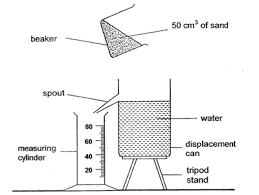
\includegraphics{eurekacan.png}
\caption{Displacement can in use.}
\end{marginfigure} 
In both cases calculate the density using: $ \rho = m/V$.
%%%%%%%%%%%%%%%%%%%%%%%%%%%%%%%%%%%%%%%%%%%%%%%%%%%%%%%%%
%\newpage
\section{Determination of unknown masses by using the principle of moments}
\subsection{Theory:}  
Apply the principle of moments to a metre rule to first determine its mass and then determine the mass of an unknown object.   
\subsection{Apparatus:} 
\begin{itemize}
\item Meter rule Clamp and stand 
\item Nail 
\item 200 g mass and hanger 
\item 150 g mass (covered in tape and labelled as W) and hanger 
\item Loops of thread           
\end{itemize}
\subsection {Experimental Method:}  
Loop a 200 g (1.96 N) mass over the metre rule and adjust it until the ruler is horizontal. Note down the distance, $x$, of the mass from the pivot. The mass (or weight) of the metre rule can now be calculated using the principle of moments:  
\begin{figure}
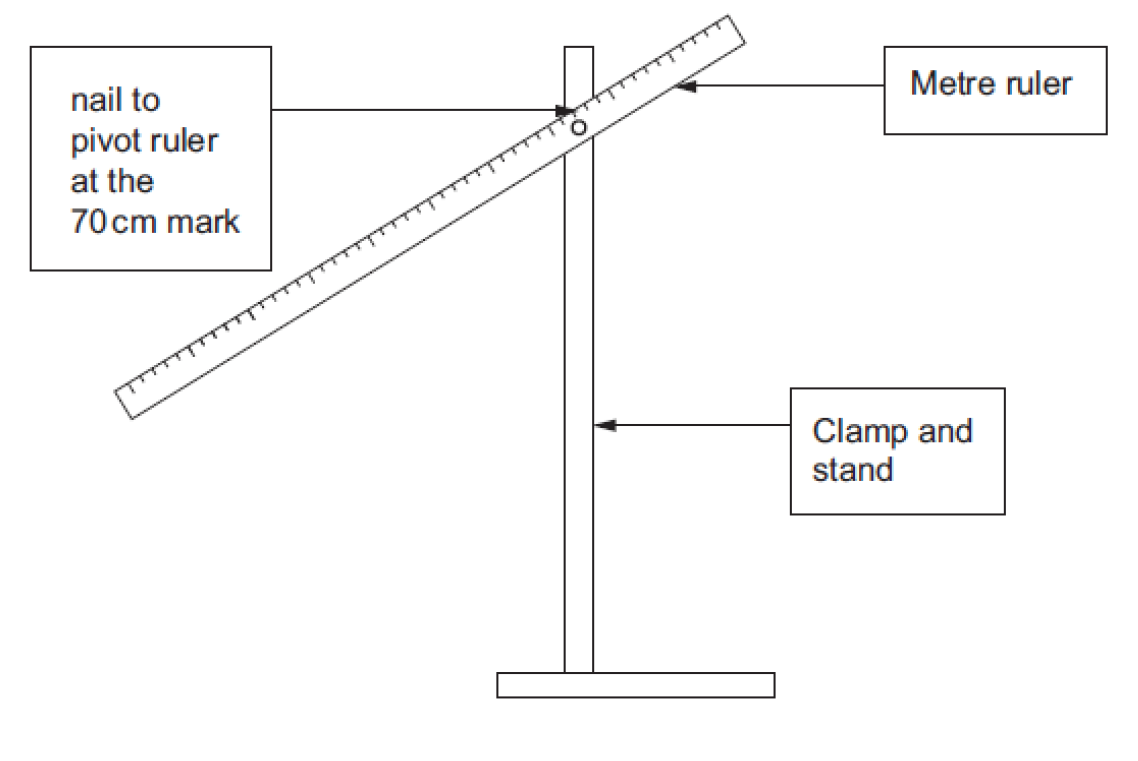
\includegraphics[width=\textwidth]{moments.PNG}
\caption{Experimental set-up for the measurement of an unknown mass by moments. It would be possible to use a knife-edge fulcrum (pivot) instead}
\end{figure}
\[0.20 \times \text{metre rule weight} = 1.96 \times x\] Now remove the 200 g mass and replace it with the unknown weight, W, and again adjust the position of the weight until the ruler balances. Measure the distance, d, of the unknown weight from the pivot. The unknown weight can again be calculated by applying the principle of moments: 

\[0.20 \times \text{metre rule weight} = d \times \text{unknown weight} \]

The unknown weight can be converted into a mass (in kilograms) by dividing by 9.81. This can then be checked using a top pan balance.\sidenote{better to use the term ``Top-pan balance'' than ``scales''} 
%%%%%%%%%%%%%%%%%%%%%%%%%%%%%%%%%%%%%%%%%%%%%%%%%%%%%%%%%%%%%%%%%%%%%
%\newpage
\section{Measurement of g by freefall}
\subsection{Theory:} 

An equation of motion can be used to calculate the acceleration due to gravity, g.\sidenote{There are two common alternative methods to the one below. 
\begin{enumerate}
\item Manual timing - This method has a lot of inherent errors, and gives poor results. One of the biggest sources is the approx 0.3s it takes to start and stop a manual timer. The next most significant are usually parallax and air resistance.
\item Using lightgates - Lightgates are very accurate, and a viable alternative for high precision results
\end{enumerate}

All of these methods rely on the same basic equations of motion} 
\begin {align} 
s &= ut + \frac{1}{2}mv^{2} \\
    Where:  u &= \text{initial velocity} = 0,   \\    s &= \text{height, h and}  \\     a &= \text{acceleration due to gravity, } g \\ 
    \text{This gives } h &= \frac{1}{2}gt^{2}\\
    \end{align}
If a graph of height, $h$, (y-axis) is plotted against time squared, $t^{2}$, (x-axis) the gradient will equal g/2, or $g = 2\times \text{gradient}$.  
\subsection{Apparatus:}  

\begin{figure}
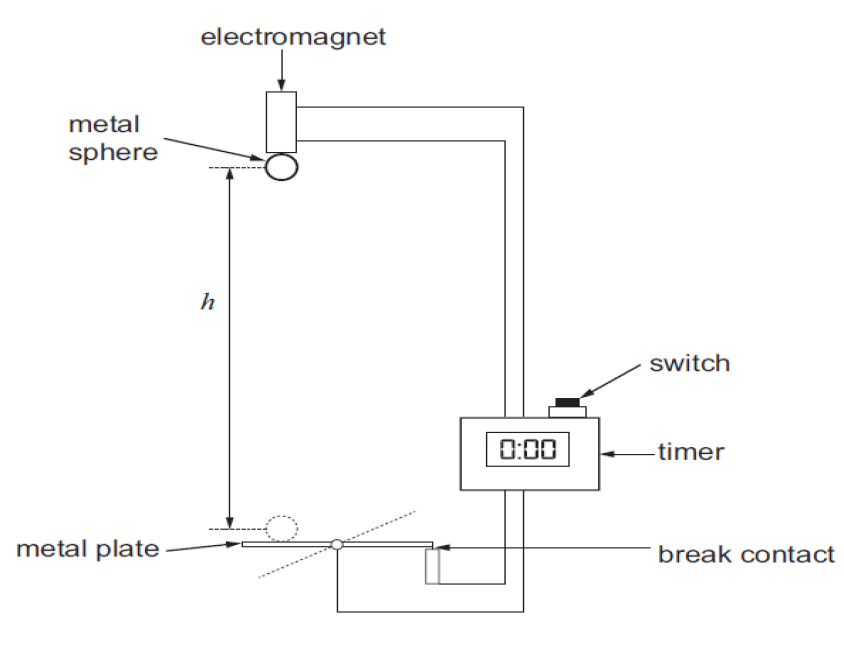
\includegraphics[width=\textwidth]{gbyfree.PNG}
\caption{``g'' by freefall}
\end{figure}

\subsection{Experimental Method:}  
When the switch is pressed it disconnects the electromagnet releasing the metal sphere\sidenote{One of the problems with this method is that the de-magnetisation of the coil is not instant. To minimise the time delay we use a soft-iron ball}. At the same instant the timer starts. When the sphere hits the magnetic switch it breaks the circuit stopping the timer, thus recording the time it takes for the sphere to fall through a height, $h$. The time taken for the ball bearing to fall through a range of different heights needs to be measured. Plot a graph of height, $h$, (y-axis) against time squared, $t^{2}$, (x-axis) and calculate the value of $g$ using:  $g = 2/gradient$. 

%%%%%%%%%%%
%\newpage
\section{Investigation of Newton's 2nd law}

\subsection{Theory:}  
The gravitational force of the slotted masses attached via the pulley causes the entire mass of the system to accelerate. That is the mass of the rider, M, and the total mass of the slotted masses, m. Newton’s second law, therefore, can be written as:  
\[mg=(M+m)a\]
and so the acceleration of the system is:  
\[a=\frac{mg}{(M+m)}\]  
We can use this to test Newton's second law. If the total mass of the system ($M + m$) remains constant\sidenote{This is \emph{really} important and is the reason that we take masses from the hanger and place them onto the car and vice-versa} then the acceleration, $a$, should be proportional to the gravitational force, $mg$.  
\subsection{Apparatus:}    
\begin{figure}
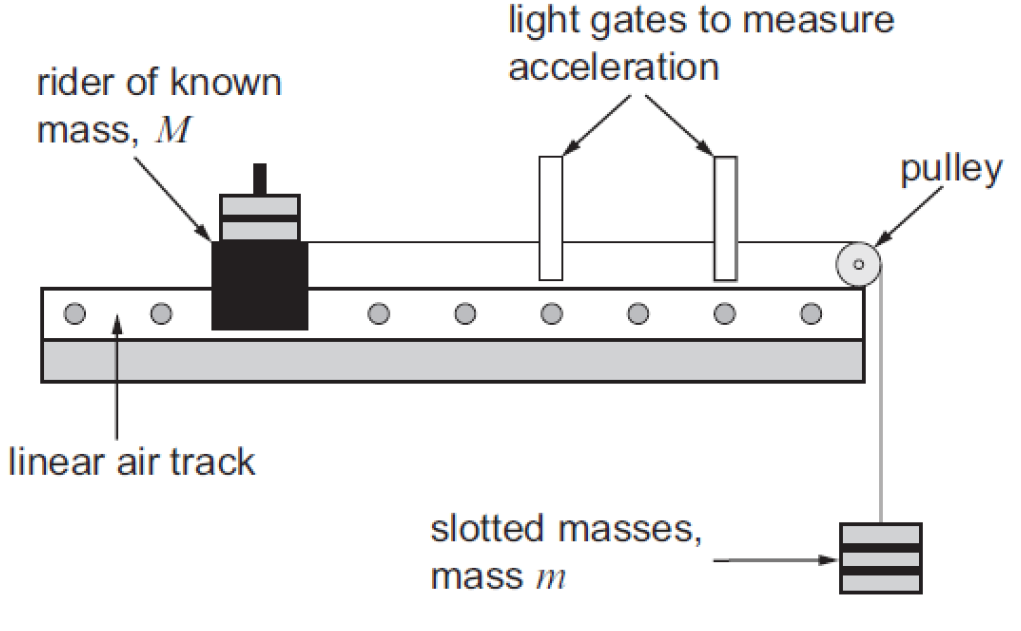
\includegraphics[width=\textwidth]{fma.PNG}
\caption{Newton's law experiment. Note that an air-track is not strictly necessary, we're trying to minimise the effect of friction on the system.}
\end{figure}
   
\subsection{Experimental Method:}  
Fix the thread to the rider and attach five slotted 5 gram masses to the other end as shown in the diagram. Set the light gates to record the acceleration and allow the slotted masses to fall to the ground. Record the gravitational force, mg and the acceleration, a. Remove one of the slotted masses and place it on the rider (so keeping the total mass of the system constant).   
Repeat the experiment until all the different accelerating masses have been removed. Plot a graph of acceleration (y-axis) against gravitational force, $mg$ (x-axis). This should be a straight line through the origin. \sidenote{By using a scales to measure the combined mass of the system $M+,m$ you could check that the gradient is equal to $1/(M+m)$}

%%%%%%%%%%%
%\newpage
\section{Determination of Young modulus of a metal in the form of a wire}

\subsection{Theory:}  $\text{Young modulus}  =\frac{\text{Stress}}{\text{Strain}}$  or $ E  =\frac{F/A}{x/l}$  rearranging $E =\frac{Fl}{xA}$ 
where: 
\begin{align}
       F &= \text{applied load} \\       A &= \text{area of cross-section of the wire} \\       x &= \text{extension}  \\      l &= \text{original length} \\ 
\end{align}
       
If a graph of applied load, F (y-axis) is drawn against extension, x (x-axis) the gradient is $\frac{F}{x}$ and so: \[E = \text{gradient} \times \frac{l}{A}\]     
The original length $l$ can be measured and the area of the wire found using $A= \pi r^{2}$ hence $E$ can be determined.  
\subsection{Apparatus:}   
  \begin{figure}
\includegraphics[width=\textwidth]{youngmod.PNG}
\caption{Young's Modulus apparatus}
\end{figure}
  
\subsection{Experimental Method:}  
Hang two identical wires from a beam and attach a scale to the first wire and a small weight to keep it straight.\sidenote{We use this method to eliminate any thermal extension/contraction} Also put a small weight on the second wire to straighten it and a Vernier scale linking with the scale on the comparison wire. Measure the original length, $l$, of the test wire and its diameter at various points along its length\sidenote{Measuring at several places along the length is a favourite of exam boards.}. Use this to calculate the mean cross sectional area $A$.  
Then place a load of {5}{N} on the test wire and find the extension, $x$. Repeat this in $5$N steps up to at least $50$N. Plot a graph of load (y-axis) against extension (x-axis) and calculate the gradient. Use this to find a value for the Young modulus. 

%%%%%%%%%%%
%\newpage
\section{Investigation of the force-extension relationship for rubber}
\subsection{Theory:}  
Rubber is an example of a polymer with weak cross bonds. Natural rubber is a polymer of the molecule iso-prene. It has weak van der Waals cross-bonds and only a few covalent (strong) cross-bonds.   
\subsection{Apparatus:} 
\begin{itemize}
\item Rubber band of cross-section approximately 1 mm by 2 mm 
\item Clamp and stand G-clamp to secure (if required) 50 g mass holder plus a number of 50 g masses 
\item Optical pin (for use as a pointer if required) 
\item Metre rule (resolution $\pm 0.001$m) Micrometer (resolution $\pm 0.01$mm)
\end{itemize}
\begin{marginfigure}
\includegraphics{hyst.jpg}
\caption{Hysteresis graph for rubber band}
\end{marginfigure}
\subsection{Experimental Method:}  
Hang a (cut) rubber band of (approximate) cross-section 1 mm by 2 mm vertically from a stand, boss and clamp. The base of the stand should be secured using a G-clamp. Hang a 50 gram mass holder from the band. Place a metre rule as close as possible to the mass holder. The length can be read using an optical pin attached to the base of the mass holder.
Measure the length, width and thickness of the rubber when it is supporting the 50 gram holder. Try to avoid squashing the rubber with the micrometer screw gauge. Increase the mass in 50 gram steps, measuring the extension each time. Continue until the band breaks.\sidenote{If, instead of testing to failure, you now unload the masses and measure the extension you can measure the elastic \emph{hysteresis} - the work done in rearranging the internal structure of the rubber.} Plot the force - extension curve and determine the Young modulus from the linear section.  
%%%%%%%%%%%
%\newpage
\section{I-V characteristics of the filament of a lamp and a metal wire at constant temperature}
\subsection{Theory:} 
Ohm's law states that for a conductor the current, I, is directly proportional to the potential difference, V, provided physical factors such as temperature and pressure remains constant.  Therefore by plotting the I-V characteristic of each of, a metal wire and a filament lamp, the validity of Ohm's law as applicable to each of these components can be determined. A graph of I against V is linear for a metal wire and non-linear for a filament of a lamp. 
\subsection{Apparatus:}
\begin {itemize}
\item Variable d.c. voltage supply 
\item Switch 
\item Ammeter 
\item Voltmeter 
\item Component either in the form of a filament bulb e.g. 12 V, 24 W bulb or a metal wire e.g. 1 m length of constantan mounted on a wooden batten 
\end{itemize}
\begin{marginfigure}
\includegraphics[]{vigraphs.png}
\caption{VI graphs of common components}
\end{marginfigure}

\subsection{Experimental method:} 
The circuit should be set up as in figure \ref{V-I}.
\begin{figure}
\includegraphics[width=\textwidth]{vicac.PNG}
\caption{V-I Characteristics set-up.\newline Note the variable powersupply and the switch. This basic circuit is used to investigate almost every electrical component}
\label{V-I}
\end{figure}

 
Starting with the output of the variable d.c. voltage supply set to its minimum value, slowly increase the value of the applied voltage. The current through the component and the potential difference across the component should be recorded for a range of values of the applied voltage. A graph of current against voltage should then be plotted. This procedure can be repeated for different components.
%%%%%%%%%%%
%\newpage
\section{Determination of the internal resistance of a cell}
\subsection{Theory:} 
\sidenote{I've tried to be quite clear here and give a bit of extra detail. Internal resistance is a favourite of examiners and I'd be amazed if this experiment didn't show up in some way}When charge flows through a cell it is given energy by the cell.
The number of joules of energy given to each coulomb of charge that passes through the cell is the e.m.f.\sidenote{e.m.f. is an abbreviation for electromotive force.} of the cell.
The energy can only be transferred to the charges at a finite rate, we model this as the cell having resistance. This model resistance is called the internal resistance of the cell. A cell can be thought of as a source of e.m.f. with a resistor connected in series.\begin{marginfigure}
\includegraphics[]{intr.jpg}
\caption{Internal resistance graph}
\end{marginfigure}
When current flows through the cell a voltage develops across the internal resistance. This voltage is not available to the circuit so it is called the lost volts, ($V_{L}$).
$V_{L}$ can also be written as $Ir$
The voltage across the ends of the cell is called the terminal potential difference, ($V_{t.p.d}$).
$V_{t.p.d}$ can also be written as $IR$
Because voltage is a measure of energy, and energy is always conserved, the e.m.f. of a cell is equal to the sum of its terminal potential difference, ($V_{t.p.d}$), and the lost volts, ($V_{L}$).
This gives rise to the equation: \[E = V_{t.p.d.}+ V_{L}\]

This equation can be written in different forms, e.g. $E = I (R + r)$

The most common form of the equation used for determining the internal resistance is $V =E-Ir$ where $V$ is the terminal p.d. of a cell; $E$ is the emf of the cell; $I$  the current flowing in the circuit and $r$ is the internal resistance.  $V = IR$ and the equation can be re-written as $ R=\frac{E}{I}-r$.  Therefore a graph of $R$ against $1/I$  should be linear.   
\subsection{Apparatus:} 
\begin{itemize}
\item Cells - e.g. 3 or 4 1.5 V `D' type batteries connected in series
\item Switch 
\item Ammeter or multimeter set to A range - {$\pm$ 0.01}{A}
\item Various resistor values 0-60$\Omega$
\end{itemize}
\subsection{Experimental method:} 
The circuit should be set-up as follows:  
\begin{figure}
\includegraphics[width=\textwidth]{internalres.PNG}
\end{figure}

The resistor values should be varied and the current values recorded. Plot a graph of $R$  (y-axis) against $1/I$  (x-axis).  The graph should be a straight line with the intercept on the y-axis which is equal to the value of the internal resistance. 
%%%%%%%%%%%
%\newpage
\section{Measurement of the intensity variations for polarisation}
\subsection{Theory:} 
The light waves in a ray of light from a lamp have vibrations in all planes and directions.  The light is unpolarised.  When the light passes through a polaroid filter; the vibrations will be in one plane or direction only.  In the experiment with two pieces of polaroid, the first polarises the light.  The light will then not pass through the second polaroid if the direction in which the second filters polarises light is at right angles to the polarising direction of the first polaroid.
\subsection{Apparatus:} \begin{itemize} 
\item Two pieces of polaroid 
\item Lamp e.g. 24 W, 12 V bulb in holder  
\end{itemize}
\subsection{Experimental method:} 
Investigate the variation in intensity by looking through the lamp through both polaroids and rotating one of the polaroids through 360 degrees.
\begin{figure}
\includegraphics[width=\textwidth]{pracfigs/malus.jpg}
\caption{Investigating the Polarisation of light. When the full version (not on the spec) is done, the intensity of light and the angle of the analyser relative to the polariser is measured. The experiment is used to test malus's law. According to malus, when completely plane polarized light is incident on the analyzer, the intensity of the light transmitted by the analyzer is directly proportional to the square of the cosine of angle between the transmission axes of the analyzer and the polarizer.}
\end{figure} 
Note the change in intensity that occurs. 
%%%%%%%%%%%
%\newpage
\section{Determination of wavelength using Young's double slits}
\subsection{Theory:} Young's interference experiment, also called Young's double-slit interferometer, was the original version of the modern double-slit experiment, performed at the beginning of the nineteenth century by Thomas Young. This experiment played a major role in the general acceptance of the wave theory of light. The fringe spacing, $\Delta y $ is given by the equation$\Delta y = \frac{\lambda D}{d}$ where $\lambda$ is the wavelength of the light; $D$ is the distance from the slits to the screen where the fringes are viewed and $d$ is the distance between the slits.  A graph of $\Delta y$ against $D$ should be a straight line and the gradient can be used to determine the wavelength of the light. 
\subsection{Apparatus:}
\begin{itemize}
\item Laser pen 
\item Stand and clamp 
\item Double slit 
\item Screen 
\item Metre rule 
\item 30 cm ruler or digital callipers
\end{itemize}
\subsection{Experimental method:} 
The apparatus should be set-up as follows:   
\begin{figure}
\includegraphics[width=\textwidth]{pracfigs/youngs.PNG}
\caption{Young's Slits experiment}
\end{figure}

Measure the fringe spacing
\begin{marginfigure}
\includegraphics[]{singledouble.jpg}
\caption{Fringe pattern for red light of 633nm.}
\end{marginfigure} $\Delta y$, the spacing between the slits, $d$, and the distance, $D$, from the slits to the screen using either the ruler or digital callipers.  Vary the distance, $D$ in equal intervals. Plot a graph of the fringe spacing $\Delta y$ (y-axis) against the slit-screen distance $D$  (x-axis). This should be a straight line through the origin.  
If the fringes are close together; $\Delta y$ can be determined by measuring the separation of a number of fringes. So determine by dividing the distance by the number of fringes measured.   
%%%%%%%%%%%
%\newpage
\section{Determination of wavelength using a diffraction grating}
\subsection{Theory:} 
The diffraction grating equation is given by $n \lambda  =d\sin \theta$. The spacing between the lines in a diffraction grating is usually specified or can be found from the grating ruling.
\begin{marginfigure}
\includegraphics[]{diffraction.jpg}
\caption{Geometry of diffraction}
\end{marginfigure} 
By measuring the angle $\theta$, the wavelength of the light can be determined. 
\subsection{Apparatus:}
\begin{itemize}
\item Laser 
\item Diffraction grating of known $d$ value or ruling e.g. 300 lines $cm^-1$ 
\item Metre rule 
\item Screen 
\item Stand and clamp for laser and grating 
\end{itemize}

\subsection{Experimental method:} 
The apparatus should be set-up as follows:  
\begin{figure}
\includegraphics[width=\textwidth]{diffractiongrating.PNG}
\caption{Diffraction grating setup}
\end{figure}
The value of $\theta$ can be determined from $\tan \theta = \frac{x}{D}$. \\ 
Using the equation $n \lambda  =d\sin \theta$ then the wavelength can be determined for various orders of diffraction. 
%%%%%%%%%%%
%\newpage
\section{Determination of the speed of sound using stationary waves}
\subsection{Theory:} 
When resonance first occurs the length of air in the tube, $l$, plus a small end correction, $e$ (to account for the position of the tuning fork above the tube) will be equal to a quarter of a wavelength. Hence: 
\[l + e = \lambda/4 \] but \[ \lambda = c/f \] so   \[l = \frac{c}{4f}-e\] If a graph is plotted of $l$ (y-axis) against $1/f$ (x-axis) it should be a straight line with a small negative y-intercept. \begin{marginfigure}
\includegraphics[]{pracfigs/waves.jpg}
\caption{Standing waves in an open ended pipe}
\end{marginfigure}
The gradient of the graph equals $c/4$, and so the speed of sound, $c$, can be found. The small negative intercept will give the end correction. 
\subsection{Apparatus:}   
\begin{figure}
\includegraphics[width=\textwidth]{pracfigs/speedsound.PNG}
\end{figure}
   
A range of at least five different tuning forks will be needed along with a metre ruler of resolution $\pm$0.001m. 
\subsection{Experimental method:}

Initially place the resonance tube as deep as possible into the water. Then gradually raise it. As this is being done hold a vibrating tuning fork over the top. When resonance occurs (a loud sound will be heard) measure the length of the tube above the water level.  Repeat the above for each of the tuning forks. Plot a graph of length (y-axis) against 1/frequency (x-axis). Use the gradient to determine a value for the speed of sound.
%%%%%%%%%%%
%\newpage
\section{Determination of resistivity of a metal}
\sidenote{There are lots of possible experiments here. So long as you are systematic in changing only one variable in $R=\frac{\rho l}{A}$}
\subsection{Theory:}  Resistivity, $\rho$ can be found using the equation $R=\frac{\rho l}{A}$ where $l$ is the length of the wire, $A$ the cross-sectional area and $R$ the resistance.\begin{marginfigure}
\includegraphics[]{resistivity.png}
\caption{Geometry of resistivity}
\end{marginfigure} This can be compared with the equation for a straight-line $ y = mx +c$. A graph plotted of $R$ (y-axis) against $l$ (x-axis) will be a straight line through the origin of gradient $\frac{\rho}{A}$. The cross sectional area can be found using $A=\pi r^{2}$ and the resistivity calculated by $ \rho = \text{gradient} \times A$.  
\subsection{Apparatus:} 
\begin{figure}
\includegraphics[width=\textwidth]{resist.PNG}
\caption{Experimental set-up for Resistivity of a wire investigation}
\end{figure}
\begin{itemize}
\item leads 
\item ammeter 
\item voltmeter 
\item 1.5 V `D' type battery 
\item metre rule 
\item 110 cm length of nichrome wire
\item 1 micrometer / vernier callipers (resolution $\pm$ 0.01mm)  
\item 30 cm ruler (resolution $\pm$ 0.001m)  
\end{itemize}
\subsection{Experimental Method:}  
Leaving one crocodile clip fixed at one end of the wire, the other clip should be moved along at suitable intervals e.g. every 10 cm / 20 cm to cover the whole range of the wire. Readings on the voltmeter and ammeter should be noted for each length and the resistance determined using $R = \frac{V}{I}$ . The diameter of the wire can be found using a micrometer or Vernier callipers and the cross-sectional area determined. Plot a graph of $R$ (y-axis) against $l$ (x-axis) and calculate the resistivity using:  $\rho = \text{gradient} \times A$. 
%%%%%%%%%%%
%\newpage
\section{Investigation of the variation of resistance with temperature for a metal wire}
\subsection{Theory:} 
Resistance increases with temperature for metals in a linear relationship. This practical will enable data to be obtained to investigate this relationship. \sidenote{A common substitution is to swap the wire in the investigation for a thermistor. Thermistors are semiconductor devices that have the reversed behaviour to normal wires. As their temperature increases, the resistance of a thermistor \emph{decreases}}.
\subsection{Apparatus:}
\begin{itemize}
\item Bunsen burner; tripod, gauze and stand 
\item 250 ml beaker of water 
\item Ice \marginnote{Because the effect of resistance change with temperature is small, it is important to cover as large a range of temperatures as is safe and practical. In an A-level lab it would be possible to get down to about -40C and up to about 1200C. These extreme temperatures are dangerous however and would need particular precautions}
\item Thermometer 0 - 100C 
\item Multimeter set on ohm range to measure resistance 
\item Copper coil 
\item Stirrer
\end{itemize}

\subsection{Experimental method:}
The circuit should be set up as follows:  
\begin{figure}
\includegraphics[width=\textwidth]{restemp.PNG}
\caption{Resistance of a wire with Temperature}
\end{figure}
The water bath should be heated and the water stirred continuously in order to ensure an even temperature throughout the water bath.  Once the required temperature has been reached then remove the heat and record the reading of resistance or take the ammeter and voltmeter readings. This process should be repeated at intervals until the water boils.  
Repeat the experiment during cooling. Plot a graph of resistance (y-axis) against temperature (x-axis). This should be a straight line through the origin.  
An ice water mixture can be used to record the resistance at a temperature of 0C. 
%%%%%%%%%%%
%\newpage
\section{Measurement of the refractive index of a material}
 \subsection{Theory:}  
The refractive index, $n$, of a material can be determined from the equation $\sin \theta_{i} = \sin \theta_{r}$ where $n$ = refractive index, $\theta_{i}$is the angle of incidence and $\theta_{r}$ is the angle of refraction. \begin{marginfigure}
\includegraphics[]{refrac.jpg}
\caption{Refractive index measurement}
\end{marginfigure} The above equation assumes that the incident ray is travelling in air.  A graph of $\sin\theta_{i}$ (y-axis) against $\sin \theta_{r}$ (x-axis) will give a straight line through the origin and the gradient is equal to the refractive index, $n$.  
\subsection{Apparatus:} 
\begin{itemize}
\item Suitable white light source e.g. ray box fitted with a single slit to produce a narrow parallel beam of light 
\item Power supply for ray box and connecting leads 
\item Rectangular block of glass or Perspex 
\item 1 or 2 sheets of plain paper 
\item Protractor 
\item 30 cm ruler
\end{itemize}
\subsection{Experimental Method:}  
The following arrangement should be set-up.  
\begin{figure}
\includegraphics[width=\textwidth]{snells.PNG}
\end{figure}
The angle of refraction $\theta_{r}$ can be measured by drawing in the line joining the incident and emergent rays for different values of the angle of incidence \sidenote{Particular care should be taken here. The more precise the drawing, the better the final results.}. The angles can be measured using the protractor after drawing in the normals\sidenote{the ``normal'' is a line at 90 degrees to a surface. In this case it is at a right angle to the glass block, as shown by a dotted line in the diagram}. A graph of $\sin\theta_{i}$ (y-axis) against$\sin \theta_{r}$(xaxis) can be plotted which should give a straight line. A value of $n$ can then be determined from the gradient. 
%%%%%%%%%%%
%\newpage
\section{Determination of h using LEDs}
\subsection{Theory:} The Planck constant, $h$, can be determined by using a light emitting diode (LED) and measuring the minimum voltage, $V_{min}$, at which light is just emitted by the diode. \sidenote{The energy levels in the LED are quantised, and they are constructed such that their emissions are monochromatic. Because energy is conserved, the only light that the LED can emit will have an energy corresponding to the energy level transition inside the material. \newline Potential difference is a measure of the energy difference between two points. The potential required to light the LED must therefore be the energy of the photons released. Photon energy is given by $E=hf$, where $h$ is planck's constant and $f$ is the frequency of light.} The Planck constant can then be determined from the equation $V_{min}=\frac{hc}{e\lambda}$  where $c$ is the speed of light $3.00e8 ms^-1$ and $e$ is the electronic charge, $1.60e-19$C.  A graph of $V_{min}$ against $1/\lambda$ should be a straight line with the gradient equal to $V_{min}=\frac{hc}{e}$. \sidenote{Many experiments have equations in the form $y=mx+c$. You should expect to have to match the variables in an equation with the parts of an equation of a straight line. It would be unsurprising to have a question requiring you to calculate gradients and Y-intercepts}

\subsection{Apparatus:} \begin{itemize}
\item Variable d.c. power supply 
\item $1 k\Omega$} protective resistor 
\item Voltmeter (resolution $\pm$ 0.01V) [multimeter set to appropriate range] 
\item Connecting leads 
\item Various LEDs - with known wavelengths
\end{itemize}
\subsection{Experimental Method:} The circuit should be set-up as follows: 
\begin{figure}
\includegraphics[width=\textwidth]{/plank.PNG}
\end{figure}

The voltage should be varied until light is just emitted by the LED. Record the voltage it corresponds to $V_{min}$. The LED should be replaced and the procedure repeated for LEDs with different wavelengths of light.  Plot a graph of $V_{min}$ (x-axis) against $1/ \lambda$  (y-axis) and use it to determine a value for $h$. 

\section{Radioactive Analogue with dice}
\subsection{Theory:}
Radioactive decay is based on the assumption that the disintegrations are entirely at random. This can be modelled using dice to represent the atoms of a radioactive isotope.\sidenote{The throwing of dice isn't a perfect model as the probability is discrete as opposed to continuous}
\subsection{Apparatus:}
\begin{itemize}

\item 100 dice or cubes with only one side coloured  \begin{marginfigure}
	\includegraphics[]{halflife.jpg}
	\caption{Half-life Dice}
\end{marginfigure}
\item 1 cup to hold dice

\end{itemize}

\subsection{Experimental Method:}
Throw the dice onto the table. Suppose all the dice with the number 1 uppermost have disintegrated. Remove these dice and count the number remaining. Repeat this for a further 9 throws (making 10 in all) and note down the number of throws and the number of dice remaining each time.
When complete combine the results of the class so you have data for approx 1000 dice rolled 10 times. \sidenote{This is worth thinking about - we want a statistically significant number of events}
Plot a graph of number of dice remaining (y-axis) against number of throws (x-axis). This should give an exponential curve with a half-life of about 3.8 throws.\\
\includegraphics[width=\textwidth]{dice.jpg}
You could use ICT such as computer modelling, or data logger with a variety of sensors to collect data, or use of software to process data.

\section{Investigation of charging and discharging a capacitor to determine the time constant}
\subsection{Theory:}
The discharge of a capacitor is given by the equation: \[Q=Q_{0}e^{-\frac{t}{RC}}\] which can be written in terms of the voltage across the capacitor as: \[V=V_{0}e^{-\frac{t}{RC}}\]
By using logs, the above equation can be written as: \[\ln{V}= \frac{-t}{RC} + \ln{V_{0}}\]
which can be compared with $y=mx+c$.
The charging of a capacitor is given by: \[V=V_{0} \left(1-e^{-\frac{t}{RC}}\right).\] \begin{marginfigure}
\includegraphics[]{charging-and-discharging-of-capacitor.PNG}
\caption{Charging and discharging graphs}
\end{marginfigure}
\subsection{Apparatus:}
\begin{itemize}
	\item d.c. power supply
\item Voltmeter (multimeter set on d.c. voltage range or CRO) - resolution $\pm$ 0.01V
\item Stopwatch - resolution - either $\pm$ 1s or $\pm$ 0.01s
\item 4mm leads
\item Suitable switches
\item Electrolytic capacitors e.g. 1000$\mu F$
\item Resistors e.g. 100 $k\Omega$} or other values

\end{itemize}

\subsection{Experimental method:}
The following circuit can be used to investigate the charging of a capacitor:\\
\includegraphics[width=\textwidth]{capcharge.PNG}
The above circuit can then be re-arranged to investigate the discharging of a capacitor as follows:\\
\includegraphics[width=\textwidth]{capdischarge.PNG}
\subsection{Charging the capacitor:}
Set up the circuit from the above diagram and by using electrolytic capacitors the correct polarity connection \begin{marginfigure}
\includegraphics[]{electrol.jpg}
\caption{An Electrolytic capacitor - It's very important to connect them correctly.}
\end{marginfigure} needs to be checked by supervisors. The two way switch needs to be in position 1 so that the capacitor can be charged and then switched over to position 2 to discharge. Pre-trial readings can be taken to determine suitable time intervals.
\subsection{Discharging the capacitor:}
The method is similar to charging the capacitor. Initially the switch is to be left open and then connected so that the capacitor charges.
\subsection{Extension:}
The value of the capacitor could be hidden and the experimental set-up used to determine its value.
The equation ($t_{1/2}=0.69R$) i.e. the time taken for the voltage to fall to half its initial value could be investigated using the data obtained.
\subsection{Data Logging:} The voltage across the capacitor can be measured using a suitable voltage sensor.

%%%%%%%%%%%%%%%%%%%%%%%%
\subsection{Investigation of the energy stored in a capacitor}
\subsection{Theory:}
The energy stored by a capacitor is given by the equation: \(U=QV\). \begin{marginfigure}
\includegraphics[]{capenergy.png}
\caption{The energy stored in a capacitor is the area under the line on a graph of V vs Q}
\end{marginfigure} 
Given that \(Q=CV\) then the equation for the energy stored can be written in the form: \(U=\frac{1}{2} CV^{2}\). The capacitor can be charged to various values of V and then the energy stored can be determined by using a Joule meter. The energy stored can be measured as the capacitor discharges. A graph of energy stored against \(V^{2}\) should be linear and the value of the capacitance can then be measured.
\subsection{Apparatus:}

\begin{itemize}
	\item d.c. power supply
	\item Voltmeter (multimeter set on d.c. voltage range or CRO) – resolution $\pm$0.01V
	\item Digital joule meter
	\item 4mm leads
	\item Suitable switches
	\item Electrolytic capacitors e.g. 1000$\mu$F 
	\item Resistors e.g. 100$k \Omega$ or other values
\end{itemize}

\subsection{Experimental method:}
The following circuit can be used \\
\includegraphics[width=\textwidth]{energycap.PNG}
Learners can set up the circuit from the above diagram and if using electrolytic capacitors the correct polarity connection needs to be checked\sidenote{There's a safety consideration here. If connected the wrong way round they can explode as the dielectric heats to boiling point}. The two switch needs to be in position 1 so that the capacitor can be charged and then switched over to position 2 to discharge.
\subsection{Extension:}
The value of the capacitor could be hidden and the experimental set-up used to determine its value.
The equation \( (t_{1/2}=0.69CR) \) i.e. the time taken for the voltage to fall to half its initial value could be investigated using the data obtained.

\subsection{Data Logging:} The voltage across the capacitor can be measured using a suitable voltage sensor.

%%%%%%%%%%%%%%%%%%%%%%%%%%%%


\section{Investigating the damping of a spring}
\subsection{Theory:}
The relationship between the amplitude of oscillation, A, and time, t, can be expressed by:
\[A=A_{0}e^{- \lambda t}\] \begin{marginfigure}
\includegraphics[]{damped.png}
\caption{Lightly damped Simple Harmonic Motion}
\end{marginfigure}
Where \(A_0\) = initial amplitude
And \(\lambda \) = an unknown constant
If we take the log of both sides we get \( \ln A = -\lambda t + \ln A_{0} \). This can be compared with the equation for a straight-line \(y = mx + c\) and so a graph of ln A against t will give a straight line of gradient \(\lambda \) and intercept ln \(A_0\).
\subsection{Apparatus:}\begin{itemize}
	
\item 500g hanger and masses
\item 2 linked springs
\item pointer
\item 2 clamps and stands
\item G-clamps (if required)
\item metre rule (resolution $\pm$0.001m)
\item stopwatch
\end{itemize}

\subsection{Experimental Method:}
\includegraphics[width=\textwidth]{damping.PNG} \begin{marginfigure}
\includegraphics[]{waterdamped.jpg}
\caption{An alternative set-up that allows for water damping.}
\end{marginfigure}
Set-up the experiment as above. Place the 500 g mass on the spring system and attach a pointer so its position can be easily read on the metre rule. Displace the mass by a further 2.5 cm.\sidenote{It's worth mentioning here that you should take care not to make any parallax errors} Let go of the mass and simultaneously start the stopwatch. Let the mass oscillate continuously and measure the new amplitude of the system every minute for the next eight minutes. Repeat this two more times and find the mean amplitude at each time. Determine ln A for each time t and plot a graph to enable you to find \(\lambda \).
\subsection{Extension:}
A series of cards of different diameters could be included to investigate the effect of different surface area on damping (the cards could be placed on top of the different masses).



\section{Investigation of the force on a current in a magnetic field}

\subsection{Theory:}
The force on a current carrying wire in a magnetic field is described by the relationship: \(F=BIl \sin \theta \).\begin{marginfigure}
\includegraphics[]{pracfigs/bil.jpg}
\caption{Flemming's left hand rule allows us to remember the effects.}
\end{marginfigure} In this practical arrangement, the value of \(\theta=90^{o} \) so the equation can be simplified to \(F=BIl\). The value of F is determined by the weight of the magnet placed on a balance. In effect \(F= \Delta mg\) where \(\Delta m \) is the apparent change in mass as F varies due to the magnitude of the current. The current can be varied and a graph of F against I can be plotted which should be linear. The length of the wire can be measured and the magnetic flux density of the magnet can be determined from the gradient of the graph and the value of length of wire within the pole pieces of the magnet.

\subsection{Apparatus:}

\begin{itemize}
\item Electronic scales with resolution {$\pm$0.001}{g}
\item Ammeter
\item Rheostat - value can be chosen so that the current can be varied in the range 0 to 3.00A or 5.00A
\item 20 SWG copper wire
\item Ammeter or mutlimeter set to A range - $\pm$ 0.01}{\ampere}
\item Variable d.c. power supply
\item U shaped soft iron section with ceramic pole pieces
\item Stand and clamp
\item Metre rule
\item length of wire

\end{itemize}

\subsection{Experimental Method:}
Set up the apparatus as shown in the diagram.\\
\includegraphics[width=\textwidth]{wireforce.PNG}
 Measure the length, l of the wire which is between the poles of the magnet. Use the rheostat to increase the current in steps from zero. For each chosen current value, record \(\Delta m\), the apparent change in mass of the magnet (this can be an increase or decrease, depending upon the orientation of the current and the magnetic field). The force, \(F\) on the wire is calculated from \(F = \Delta mg\) for each value of current I. A graph of F (y-axis) against I (x-axis) should be a straight line through the origin. The magnetic flux density, B of the magnet can be determined from: B= gradient/length of wire

\section{Measurement of specific heat capacity}
\subsection{Theory:}
Assuming no energy losses: \marginnote{%

Some typical values for specific heat capacity:\\
	\begin{tabular}{cc}
	Substance	& \(c/J Kg^{-1}K^{-1} \)  
	  \\
		Aluminium & 900  \\
		 Ice  &2100   \\
	Iron	& 450  \\
	  Wood & 1700  \\
	Copper	&  390\\
	 Water & 4186  
	\end{tabular}

}%
Electrical energy supplied by the heater = heat received by the block
\[ItV = mc(\theta_{2} - \theta_{1})\]
Where c = specific heat capacity and \((\theta_{2} - \theta_{1}) = 30^{o}\text{C}\). Hence:
\[\frac{ItV}{30m}\]
\subsection{Apparatus:}
In addition to the apparatus shown in the diagram a balance and a stopwatch are needed.

Blocks pre-drilled and with surrounding insulation are usually provided, having been specially made for the purpose. A few drops of glycerol could be placed in the thermometer hole to improve thermal contact with the block \sidenote{Failing to do this step results in poor readings from the thermometer and is a major source of error in this practical}.
\subsection{Experimental Method:}
\includegraphics[width=\textwidth]{specificheatsolid.PNG}
Use a cylindrical block of the metal to be tested (such as copper or aluminium). The block should be well lagged using an insulator such as polystyrene \sidenote{Failing to properly insulate the block will cause energy to be lost to the surrounding, spoiling the result} and it needs two pre- drilled holes, one for a heater and one for a thermometer. Measure the mass, m, of the block and record its initial temperature, \(\theta_1\). Switch the heater on and start the stopwatch. Record the voltmeter and ammeter readings. When the temperature has risen by \(30^{o}\)C switch the heater off and record the time taken, t. The formula can then be used to determine a value for c.
\subsection{Extension:}
By comparing the specific heat capacity to known constants it is possible to determine the type of metal the block is made from.

\section{Estimation of absolute zero by use of the gas laws (Charles' Law)}
\subsection{Theory:}
Charles' law states that for a constant amount of gas, the volume is proportional to the absolute temperature if the pressure remains constant. \begin{marginfigure}
\includegraphics[]{charleslaw.jpg}
\caption{Extrapolating from Charles' law to absolute zero}
\label{zero}
\end{marginfigure}
\[V \propto T\text{ for constant }P\]
A plot of volume versus Centigrade temperature intercepts the x-axis at -273 oC which suggests that the gas would occupy no volume at this temperature. This theoretical value is known as absolute zero, and is also known as 0 Kelvin.
\subsection{Apparatus:}

A small bead of concentrated sulfuric acid can be trapped in a capillary tube by first heating the tube with boiling water.\begin{marginfigure}
	\includegraphics[]{sulphur.jpg}
	\caption{We use concentrated sulphuric as it is hygroscopic - it absorbs the moisture from the trapped air bubble - this ir more dangerous than using water however it prevents the water vapour in the air bubble from giving us a poor result. It would also be a great safety point to mention!}
\end{marginfigure} When the air cools down it contracts and the sulfuric acid will move down the tube.

\subsection{Experimental Method:}
\includegraphics[width=\textwidth]{charles.PNG}
Heat the water using a Bunsen burner and stir regularly. Measure the length of the trapped air every \(10^o\)C up to \(80^o\)C. Plot a graph of the length of trapped air (y-axis) against temperature (x-axis). The temperature scale should cover the range \(-400^o\)C to
\(100^o\)C. The length scale should start at zero. Draw a line of best fit extended back until it cuts the x-axis, this is absolute zero.\sidenote{See figure \ref{zero}}
\subsection{Extension:}
The pressure law will also give a value for absolute zero. Air trapped in a flask can be heated in a water bath and the pressure measured using a pressure gauge. A graph of pressure (y-axis) against Centigrade temperature (x-axis) can be extrapolated back to give a value for absolute zero.

\section{Investigation of magnetic flux density using a hall probe}
\subsection{Theory:}
A Hall probe is a slice of doped  semiconductor with a connecting wire at each end to provide a steady current.\begin{marginfigure}
	\includegraphics[]{hallprobe.png}
	\caption{A schematic of a Hall probe.}
\end{marginfigure} Another two wires are connected across the edges of the slice to allow the Hall potential difference, \(V_H\) to be measured. Note that the slice must be placed so that it is at right angles to the magnetic field lines.\begin{marginfigure}
\includegraphics[]{sole.png}
\caption {Showing the placement of a hall probe so as to make the wafer perpendicular to the field lines - Note that the hall probes we used in class do not have this orientation, they are made of a combination of two perpendicular slices so as to work in either orientation.}
\end{marginfigure} When a constant current flows the Hall pd is proportional to the magnetic field strength, and so can be calibrated using a known magnetic field.
\begin{marginfigure}
	\includegraphics[]{solmag.jpg}
	\caption{Showing the magnetic field in a solenoid}
\end{marginfigure}
\subsection{Apparatus:}
\begin{itemize}
	\item Hall probe
\item Solenoid
\item Voltmeter
\item Ammeter
\item d.c. supply
\item Magnet of known magnetic field strength
\end{itemize}
\subsection{Experimental Method:}
Place the Hall probe into a known magnetic field, \(B_{1}\) and note the Hall potential difference, \(V_{1}\). Then place the Hall probe in the centre of a solenoid. Ensure, in both cases, the probe is perpendicular to the magnetic field. Again measure the Hall potential difference, \(V_2\) when the probe is in the solenoid. The unknown magnetic field of the solenoid, \(B_2\), can be found using:
\[B_{2} = \frac{B_{1}}{V_{1}}V_{2} \]
\subsection{Extension:}
A graph of field strength against distance along the solenoid could be drawn to show the difference in magnetic field at the ends. It is also possible to investigate the variation of magnetic field strength with the solenoid diameter.
%\chapter{Ticklists}
\section{Newtonian Physics}

Written examination: 2 hours 15 minutes
31.25\% of qualification
\subsection{Basic Physics}
Learners should be able to demonstrate and apply their knowledge and
understanding of:
\begin{itemize}
	\item[\Large{$\Square$}](a) the 6 essential base SI units (\sq kg, \sq m, \sq s, \sq A, \sq mol, \sq K)
	\item[\Large{$\Square$}](b) representing units in terms of the 6 base SI units and their prefixes
	\item[\Large{$\Square$}](c) checking equations for homogeneity using units
	\item[\Large{$\Square$}](d) the difference between scalar and vector quantities and to \sq give examples of each – displacement, velocity, acceleration, force, speed, time, density,
	pressure etc
	\item[\Large{$\Square$}](e) the addition and subtraction of coplanar vectors, and \sq perform mathematical calculations limited to \textbf{two} perpendicular vectors
	\item[\Large{$\Square$}](f) how to resolve a vector into two perpendicular components
	\item[\Large{$\Square$}](g) the concept of density and \sq how to use the equation \(\rho=\frac{m}{V}\) to calculate mass, density and volume
	\item[\Large{$\Square$}](h) what is meant by the turning effect of a force
	\item[\Large{$\Square$}](i) the use of the principle of moments
	\item[\Large{$\Square$}](j) the use of centre of gravity, for example in problems including stability:
	identify its position in a \sq cylinder, \sq sphere and \sq cuboid (beam) of uniform density
	\item[\Large{$\Square$}](k) when a body is in equilibrium the resultant force is zero and the net moment
	is zero, and \sq be able to perform simple calculations
	\subsection*{SPECIFIED PRACTICAL WORK}
	\item[\Large{$\Square$}] Measurement of the density of solids
	\item[\Large{$\Square$}] Determination of unknown masses by using the principle of moments
\end{itemize}
\subsection{Kinematics}
Learners should be able to demonstrate and apply their knowledge and
understanding of:
\begin{itemize}
	\item[\Large{$\Square$}](a) what is meant by \sq displacement, mean and instantaneous values of \sq speed, \sq velocity and \sq acceleration
	\item[\Large{$\Square$}](b) the representation of \sq displacement, \sq speed, \sq velocity and \sq acceleration by graphical methods
	\item[\Large{$\Square$}](c) the properties of \sq displacement-time graphs, \sq velocity-time graphs, and \sq interpret speed and displacement-time graphs for non-uniform acceleration
	\item[\Large{$\Square$}](d) how to derive and use equations which represent uniformly accelerated
	motion in a straight line
	\item[\Large{$\Square$}](e) how to describe the motion of bodies falling in a gravitational field \sq with and \sq without air resistance - terminal velocity
	\item[\Large{$\Square$}](f) the independence of vertical and horizontal motion of a body moving freely under gravity
	\item[\Large{$\Square$}](g) the explanation of the motion due to a uniform velocity in one direction and uniform acceleration in a perpendicular direction, and \sq perform simple
	calculations
	\subsection*{SPECIFIED PRACTICAL WORK}
	\item[\Large{$\Square$}] Measurement of \textit{g} by freefall
\end{itemize}
\subsection{Dynamics}
Learners should be able to demonstrate and apply their knowledge and
understanding of:
\begin{itemize}
	\item[\Large{$\Square$}](a) the concept of force and Newton's \(3^{\text{rd}}\) law of motion
	\item[\Large{$\Square$}](b) how free body diagrams can be used to represent forces on a particle or body
	\item[\Large{$\Square$}](c) the use of the relationship \(\Sigma F = ma\) in situations where mass is constant
	\item[\Large{$\Square$}](d) the idea that linear momentum is the product of mass and velocity
	\item[\Large{$\Square$}](e) the concept that force is the rate of change of momentum, applying this in situations where mass is constant
	\item[\Large{$\Square$}](f) the principle of conservation of momentum and use it to solve problems in one dimension involving \sq elastic collisions (where there is no loss of kinetic
	energy) and \sq inelastic collisions (where there is a loss of kinetic energy)
	\subsection*{SPECIFIED PRACTICAL WORK}
	\item[\Large{$\Square$}]Investigation of Newton’s \(2^{\text{nd}}\) law
\end{itemize}
\subsection{Energy Concepts}
Learners should be able to demonstrate and apply their knowledge and
understanding of:
\begin{itemize}
	\item[\Large{$\Square$}](a) the idea that work is the product of a force and distance moved in the
	direction of the force when the force is constant
	\item[\Large{$\Square$}](b) the calculation of the work done for constant forces, when the force is not along the line of motion (\(\text{work done} = Fx \cos \theta \))
	\item[\Large{$\Square$}](c) the principle of conservation of energy including knowledge of \sq gravitational potential energy (\(mg \Delta h\)) , \sq elastic potential energy (\(\frac{1}{2}kx^{2}\))  and \sq kinetic energy (\(\frac{1}{2}mv^{2}\))
	\item[\Large{$\Square$}](d) the work-energy relationship:\( Fx=\frac{1}{2}mv^{2}-\frac{1}{2}mv^{2}\)
	\item[\Large{$\Square$}](e) power being the rate of energy transfer
	\item[\Large{$\Square$}](f) dissipative forces for example, friction and drag cause energy to be
	transferred from a system and reduce the overall efficiency of the system
	\item[\Large{$\Square$}](g) the equation: $\text{efficiency} = \frac{\text{useful energy transfer}}{\text{total energy input}} \times 100\% $
	
\end{itemize}
\subsection{Circular Motion}
Learners should be able to demonstrate and apply their knowledge and
understanding of:
\begin{itemize}
	\item[\Large{$\Square$}](a) the terms \sq period of rotation, \sq frequency
	\item[\Large{$\Square$}](b) the definition of the unit radian as a measure of angle
	\item[\Large{$\Square$}](c) the use of the radian as a measure of angle
	\item[\Large{$\Square$}](d) the definition of angular velocity, $\omega$, for an object performing \sq circular motion and performing \sq simple harmonic motion
	\item[\Large{$\Square$}](e) the idea that the centripetal force is the resultant force acting on a body moving at constant speed in a circle
	\item[\Large{$\Square$}](f) the centripetal force and acceleration are directed towards the centre of the circular motion
	\item[\Large{$\Square$}](g) the use of the following equations relating to circular motion:
	\[\begin{aligned}
	\text{\sq} v=\omega r, &\text{\sq} a=\omega^{2} r, & \text{\sq} a=\frac{v^{2}}{r},& \text{\sq} F=\frac{mv^{2}}{r},&\text{\sq } F=m\omega^{2}r
	\end{aligned}
	\]
	
	
\end{itemize}
\subsection{Vibrations}
Learners should be able to demonstrate and apply their knowledge and
understanding of:
\begin{itemize}
	\item[\Large{$\Square$}](a) the definition of simple harmonic motion as a statement in words
	\item[\Large{$\Square$}](b) \(a=-\omega^{2} x\) as a mathematical defining equation of simple harmonic motion.
	\item[\Large{$\Square$}](c) the graphical representation of the variation of acceleration with displacement during simple harmonic motion
	\item[\Large{$\Square$}](d) \(x=A\cos(\omega t + \epsilon) \) as a solution to \(a=-\omega^{2} x\)
	\item[\Large{$\Square$}](e) the terms \sq frequency, \sq period, \sq amplitude and \sq phase
	\item[\Large{$\Square$}](f) period as \(\frac{1}{f}\) or \(\frac{2\pi}{\omega}\)
	\item[\Large{$\Square$}](g)  \(v=A\omega\sin(\omega t + \epsilon)\) for the velocity during simple harmonic motion
	\item[\Large{$\Square$}](h) the graphical representation of the changes in \sq displacement and \sq velocity with time during simple harmonic motion
	\item[\Large{$\Square$}](i) the equation \(T=2\pi \sqrt{\frac{m}{k}}\) for the period of a system having stiffness (force per unit extension) k and mass m
	\item[\Large{$\Square$}](j) the equation \(T=2\pi \sqrt{\frac{l}{g}}\) for the period of a simple pendulum
	\item[\Large{$\Square$}](k) the graphical representation of the interchange between kinetic energy and potential energy during undamped simple harmonic motion, and \sq perform simple calculations on energy changes
	\item[\Large{$\Square$}](l) free oscillations and the effect of damping in real systems
	\item[\Large{$\Square$}](m) practical examples of damped oscillations
	\item[\Large{$\Square$}](n) the importance of critical damping in appropriate cases such as vehicle
	suspensions
	\item[\Large{$\Square$}](o) forced oscillations and resonance, and to \sq describe practical examples
	\item[\Large{$\Square$}](p) the variation of the amplitude of a forced oscillation with driving frequency and \sq that increased damping broadens the resonance curve
	\item[\Large{$\Square$}](q) circumstances when resonance is useful for example, circuit tuning,
	microwave cooking and other circumstances in which it should be avoided for example, bridge design
	\subsection*{SPECIFIED PRACTICAL WORK}
	\item[\Large{$\Square$}] Measurement of g with a pendulum
	\item[\Large{$\Square$}] Investigation of the damping of a spring
\end{itemize}
\subsection{Kinetic Theory}
Learners should be able to demonstrate and apply their knowledge and
understanding of:
\begin{itemize}
	\item[\Large{$\Square$}](a) the equation of state for an ideal gas expressed as $pV = nRT$ where R is the 	molar gas constant and $pV = NkT$ where k is the Boltzmann constant
	\item[\Large{$\Square$}](b) the assumptions of the kinetic theory of gases which includes the random distribution of energy among the molecules
	\item[\Large{$\Square$}]	(c) the idea that molecular movement causes the pressure exerted by a gas, and \sq the use of \(p=\frac{1}{3}\rho \bar{c^{2}} = \frac{1}{3}\frac{N}{V} m\bar{c^{2}}\) where N is the number of molecules
	\item[\Large{$\Square$}]	(d) the definition of Avogadro constant $N_A$ and hence the mole
	\item[\Large{$\Square$}]	(e) the idea that the molar mass $M$ is related to the relative molecular mass $M_r$ by \(M/kg=\frac{M_{r}}{1000}\), and that \sq the number of moles $n$ is given by $	\frac{\text{total mass}}{\text{molar mass}}$
	\item[\Large{$\Square$}]	(f) how to combine \(pV=\frac{1}{3}Nm\bar{C^{2}} \) with \(pV = nRT\) and show that the total translational kinetic energy of a mole of a monatomic gas is given by \(\frac{3}{2}RT\) and \sq the mean kinetic energy of a molecule is \(\frac{3}{2}kT\) where \(k=\frac{R}{N_{A}}\) is the Boltzmann constant, and that T is proportional to the mean kinetic energy
\end{itemize}
\subsection{Thermal Physics}
Learners should be able to demonstrate and apply their knowledge and
understanding of:
\begin{itemize}
	\item[\Large{$\Square$}] (a) the idea that the internal energy of a system is the sum of the potential and kinetic energies of its molecules
	\item[\Large{$\Square$}] (b) absolute zero being the temperature of a system when it has minimum
	internal energy
	\item[\Large{$\Square$}]	(c) the internal energy of an ideal monatomic gas being wholly kinetic so it is given by \(U=\frac{3}{2}nRT\)
	\item[\Large{$\Square$}]	(d) the idea that heat enters or leaves a system through its boundary or container wall, according to whether the system's temperature is lower or higher than
	that of its surroundings, so heat is energy in transit and not contained within
	the system
	\item[\Large{$\Square$}]	(e) the idea that if no heat flows between systems in contact, then they are said to be in thermal equilibrium, and are at the same temperature
	\item[\Large{$\Square$}]	(f) the idea that energy can enter or leave a system by means of work, so work is also energy in transit
	\item[\Large{$\Square$}]	(g) the equation $W = p \Delta V $ can be used to calculate the work done by a gas under constant pressure
	\item[\Large{$\Square$}]	(h) the idea that even if $p$ changes, $W$ is given by the area under the $p – V$ graph
	\item[\Large{$\Square$}]	(i) the use of the first law of thermodynamics, in the form $\Delta U=Q-W $ and \sq know how to interpret negative values of $\Delta U $, $Q$, and $W$
	\item[\Large{$\Square$}]	(j) the idea that for a solid (or liquid), $W$ is usually negligible, so $Q = \Delta U$
	\item[\Large{$\Square$}]	(k) \(Q=mc\Delta \theta\) , for a solid or liquid, and this is the defining equation for specific	heat capacity, $ c $
	\subsection*{SPECIFIED PRACTICAL WORK}
	\item[\Large{$\Square$}] Estimation of absolute zero by use of the gas laws
	\item[\Large{$\Square$}] Measurement of the specific heat capacity for a solid
\end{itemize}
\section{Electricity and the Universe}
Written examination: 2 hours
31.25\% of qualification
\subsection{Conduction of Electricity}Learners should be able to demonstrate and apply their knowledge and
understanding of:
\begin{itemize}
	\item[\Large{$\Square$}]	(a) the fact that the unit of charge is the coulomb (C), and \sq an electron's charge, $e$,	is a very small fraction of a coulomb
	\item[\Large{$\Square$}]	(b) the fact that charge can flow through certain materials, called conductors
	\item[\Large{$\Square$}]	(c) electric current being the rate of flow of charge
	\item[\Large{$\Square$}]	(d) the use of the equation \(I=\frac{\Delta Q}{\Delta t}\)
	\item[\Large{$\Square$}]	(e) current being measured in ampères (A), where $A = C s^{-1}$
	\item[\Large{$\Square$}]	(f) the mechanism of conduction in metals as the drift of free electrons
	\item[\Large{$\Square$}]	(g) the derivation and use of the equation $I = nAve$ for free electrons
\end{itemize}
\subsection{Resistance}Learners should be able to demonstrate and apply their knowledge and
understanding of:
\begin{itemize}
	\item[\Large{$\Square$}] (a) the definition of potential difference
	\item[\Large{$\Square$}]	(b) the idea that potential difference is measured in volts (V) where $V = J C^{-1}$
	\item[\Large{$\Square$}]	(c) the characteristics of I – V graphs for \sq the filament of a lamp, and \sq a metal wire at constant temperature
	\item[\Large{$\Square$}]	(d) Ohm's law, the equation \(V = IR\) and the definition of resistance
	\item[\Large{$\Square$}]	(e) resistance being measured in ohms ($\Omega$), where $\Omega = V A^{-1}$
	\item[\Large{$\Square$}]	(f) the application of \(P=IV=I^{2}R=\frac{V^{2}}{R}\)
	\item[\Large{$\Square$}]	(g) collisions between free electrons and ions gives rise to electrical resistance, and \sq electrical resistance increases with temperature
	\item[\Large{$\Square$}]	(h) the application of \(R=\frac{\rho l}{A}\) , the equation for resistivity
	\item[\Large{$\Square$}]	(i) the idea that the resistance of metals varies almost linearly with temperature	over a wide range
	\item[\Large{$\Square$}]	(j) the idea that ordinarily, collisions between free electrons and ions in metals increase the random vibration energy of the ions, so the temperature of the
	metal increases
	\item[\Large{$\Square$}]	(k) what is meant by \sq superconductivity, and \sq superconducting transition temperature
	\item[\Large{$\Square$}]	(l) the fact that most metals show superconductivity, and have transition temperatures a few degrees above absolute zero ($–273 C$)
	\item[\Large{$\Square$}]	(m) certain materials (high temperature superconductors) having transition temperatures above the boiling point of nitrogen ($–196 C$)
	\item[\Large{$\Square$}]	(n) some uses of superconductors for example, MRI scanners and particle
	accelerators
	\subsection*{SPECIFIED PRACTICAL WORK}
	\item[\Large{$\Square$}]Investigation of the I-V characteristics of the filament of a lamp and a metal wire at constant temperature
	\item[\Large{$\Square$}] Determination of resistivity of a metal
	\item[\Large{$\Square$}]Investigation of the variation of resistance with temperature for a metal wire
\end{itemize}
\subsection{D.C. Circuits}Learners should be able to demonstrate and apply their knowledge and
understanding of:
\begin{itemize}
	\item[\Large{$\Square$}](a) the idea that the current from a source is equal to the sum of the currents in	the separate branches of a parallel circuit, and that \sq this is a consequence of
	conservation of charge
	\item[\Large{$\Square$}]	(b) the sum of the potential differences across components in a series circuit is	equal to the potential difference across the supply, and that \sq this is a	consequence of conservation of energy
	\item[\Large{$\Square$}]	(c) potential differences across components in parallel are equal
	\item[\Large{$\Square$}]	(d) the application of equations for the combined resistance of resistors in \sq series	and \sq parallel
	\item[\Large{$\Square$}]	(e) the use of a potential divider in circuits (including circuits which contain \sq LDRs and \sq thermistors)
	\item[\Large{$\Square$}]	(f) what is meant by the emf of a source
	\item[\Large{$\Square$}]	(g) the unit of emf is the volt (V), which is the same as that of potential difference
	\item[\Large{$\Square$}]	(h) the idea that sources have internal resistance and to use the equation \(V=E-Ir\)
	\item[\Large{$\Square$}]	(i) how to calculate current and potential difference in a circuit containing one cell or cells in series
	\subsection*{SPECIFIED PRACTICAL WORK}
	\item[\Large{$\Square$}] Determination of the internal resistance of a cell
\end{itemize}
\subsection{Capacitance}Learners should be able to demonstrate and apply their knowledge and
understanding of:
\begin{itemize}
	\item[\Large{$\Square$}] (a) the idea that a simple parallel plate capacitor consists of a pair of equal parallel metal plates separated by a vacuum or air
	\item[\Large{$\Square$}]		(b) a capacitor storing energy by transferring charge from one plate to the other,	so that the plates carry equal but opposite charges (the net charge being zero)
	\item[\Large{$\Square$}]		(c) the definition of capacitance as \(C=\frac{Q}{V}\)
	\item[\Large{$\Square$}]		(d) the use of \(C=\frac{\epsilon_{0} A}{d}\) for a parallel plate capacitor, with no dielectric
	\item[\Large{$\Square$}]		(e) the idea that a dielectric increases the capacitance of a vacuum-spaced
	capacitor
	\item[\Large{$\Square$}]		(f) the $E$ field within a parallel plate capacitor being uniform and the use of the
	equation \(E=\frac{V}{d}\)
	\item[\Large{$\Square$}]	(g) the equation \(U=\frac{1}{2}QV \) for the energy stored in a capacitor
	\item[\Large{$\Square$}]		(h) the equations for capacitors in \sq series and in \sq parallel
	\item[\Large{$\Square$}]		(i) the process by which a capacitor charges and discharges through a resistor
	\item[\Large{$\Square$}]		(j) the equations: \sq \(Q=Q_{0} \left( 1-e^{-\frac{t}{RC}}\right) \) and \sq \(Q=Q_{0}e^{-\frac{t}{RC}} \) where RC is the time
	constant
	\subsection*{SPECIFIED PRACTICAL WORK}
	\item[\Large{$\Square$}] Investigation of the charging and discharging of a capacitor to determine the	time constant
	\item[\Large{$\Square$}]Investigation of the energy stored in a capacitor
\end{itemize}
\subsection{Solids Under Stress}Learners should be able to demonstrate and apply their knowledge and
understanding of:
\begin{itemize}
	\item[\Large{$\Square$}] (a) Hooke’s law and use \(F=kx\) where the spring constant k is the force per unit
	extension
	\item[\Large{$\Square$}]	(b) the ideas that for materials the tensile stress, \sq \(\sigma=\frac{F}{A}\) and the tensile strain, \sq \(\epsilon= \frac{\Delta l}{l}  \)
	and the Young modulus, \sq \(E=\frac{\sigma}{\epsilon}  \) when Hooke’s law applies
	\item[\Large{$\Square$}]		(c) the work done in deforming a solid being equal to the area under a force-extension graph, which is \(\frac{1}{2} Fx\) if Hooke’s law is obeyed
	\item[\Large{$\Square$}]		(d) the classification of solids as \sq crystalline, \sq amorphous (to include glasses and ceramics) and \sq polymeric
	\item[\Large{$\Square$}]	(e) the features of a force-extension (or stress-strain) graph for a metal such as	copper, to include
	\begin{itemize}
		\item[\Large{$\Square$}] elastic and \sq plastic strain
		\item[\Large{$\Square$}] the effects of dislocations, and the strengthening of metals by introducing barriers to dislocation movement, such as foreign atoms, other dislocations, and more grain boundaries
		\item[\Large{$\Square$}] necking and ductile fracture
	\end{itemize}
	\item[\Large{$\Square$}](f) the features of a force-extension (or stress-strain) graph for a brittle material such as glass, to include:
	\begin{itemize}
		\item[\Large{$\Square$}] elastic strain and obeying Hooke’s law up to fracture
		\item[\Large{$\Square$}] brittle fracture by crack propagation, the effect of surface imperfections on breaking stress, and \sq how breaking stress can be increased by reducing surface imperfections (as in thin fibres) or by \sq putting surface under compression (as in toughened glass or pre-stressed	concrete)
	\end{itemize}
	\item[\Large{$\Square$}](g) the features of a force-extension (or stress-strain) graph for rubber, to include
	\begin{itemize}
		\item Hooke’s law only approximately obeyed, low Young modulus and the \sq extension due to straightening of chain molecules against thermal opposition
		\item hysteresis
	\end{itemize}	
	\subsection*{SPECIFIED PRACTICAL WORK}
	\item[\Large{$\Square$}] Determination of Young modulus of a metal in the form of a wire
	\item[\Large{$\Square$}] Investigation of the force-extension relationship for rubber
\end{itemize}
\subsection{Electrostatic and Gravitational Fields of Force}Learners should be able to demonstrate and apply their knowledge and
understanding of:
\begin{itemize}
	\item[\Large{$\Square$}] (a) the features of electric and gravitational fields as specified in figure~\ref{fieldtab}
	\begin{figure}
		\centering
		\label{fieldtab}
		\begin{tabular}{p{0.4\textwidth} p{0.4\textwidth}}
			\toprule
			\textbf{Electric Fields}                                                 & \textbf{Gravitational fields}    \\ \midrule
			\begin{Large}$\Square$\end{Large} Electric field strength, $E$, is the force per unit charge on a small positive test charge placed at the point     & \begin{Large}$\Square$\end{Large} Gravitational field strength, g, is the force per
			unit mass on a small test mass placed at the
			point                                        \\ \midrule
			\begin{Large}$\Square$\end{Large} Inverse square law for the force between two electric charges in the form: \[F=\frac{1}{4 \pi \epsilon_{0}}\frac{Q_{1}Q_{2}}{r^2}\]
			(Coulomb's law) & \begin{Large}$\Square$\end{Large} Inverse square law for the force between two masses in the form: \[F=G\frac{M_{1}M_{2}}{r^2}\]
			(Newton's law of gravitation) \\ \midrule
			\begin{Large}$\Square$\end{Large} $F$ can be attractive or repulsive       & \begin{Large}$\Square$\end{Large} $F$ is attractive only                                                                                                                      \\ \midrule
			\begin{Large}$\Square$\end{Large} \[E=\frac{1}{4 \pi \epsilon_{0}}\frac{Q}{r^2}\]  for the field strength due to a point charge in free space or air     &\begin{Large}$\Square$\end{Large} \[g=\frac{GM}{r^2}\] for the field strength due to a point mass                                                                             \\ \midrule
			\begin{Large}$\Square$\end{Large} Potential at a point due to a point charge in terms of the work done in bringing a unit positive charge from infinity to that point & \begin{Large}$\Square$\end{Large} Potential at a point due to a point charge in terms of the work done in bringing a unit positive charge from infinity to that point \\ \midrule
			\begin{Large}$\Square$\end{Large} \[V_{E}=\frac{1}{4 \pi \epsilon_{0}}\frac{Q}{r}\] and \[PE=\frac{1}{4 \pi \epsilon_{0}}\frac{Q_{1}Q_{2}}{r}\] & \begin{Large}$\Square$\end{Large} \[V_{g}=-\frac{GM}{r}\] and \[PE=-\frac{GM_{1}M_{2}}{r}\] \\ \midrule
			\begin{Large}$\Square$\end{Large} Change in potential energy of
			a point charge moving in any electric field
			$= q \Delta V_{E}$  & \begin{Large}$\Square$\end{Large} Change in potential energy of a point mass moving in any gravitational field $= m \Delta V_{g}$\\ \midrule 
			\begin{Large}$\Square$\end{Large} Field strength at a point is
			given by
			$E = - \text{slope of the }V_{E}-r$ graph at that point & \begin{Large}$\Square$\end{Large} Field strength at a point is given by $g = - \text{ slope of the }V_{g}-r$ graph at that point \\ \bottomrule
		\end{tabular}
		\caption{Fields Table}
	\end{figure}
	\item[\Large{$\Square$}]		(b) the idea that the gravitational field outside spherical bodies such as the Earth is essentially the same as if the whole mass were concentrated at the centre
	\item[\Large{$\Square$}]		(c) field lines (or lines of force) giving the direction of the field at a point, thus, for	a positive point charge, the field lines are radially outward
	\item[\Large{$\Square$}]		(d) equipotential surfaces joining points of equal potential and are therefore spherical for a point charge
	\item[\Large{$\Square$}]		(e) how to calculate the net potential and resultant field strength for a number of point charges or point masses
	\item[\Large{$\Square$}]		(f) the equation $\Delta U_{P} = mg\Delta h$ for distances over which the variation of g is	negligible
\end{itemize}
\subsection{Using Radiation to Investigate Stars}Learners should be able to demonstrate and apply their knowledge and
understanding of:
\begin{itemize}
	\item[\Large{$\Square$}] (a) the idea that the stellar spectrum consists of a continuous emission spectrum, from the dense gas of the surface of the star, and a line absorption spectrum arising from the passage of the emitted electromagnetic radiation through the tenuous atmosphere of the star
	\item[\Large{$\Square$}]		(b) the idea that bodies which absorb all incident radiation are known as black bodies and that \sq stars are very good approximations to black bodies
	\item[\Large{$\Square$}]		(c) the shape of the black body spectrum and that the peak wavelength is inversely proportional to the absolute temperature (defined by:
	\(T (K) = \theta (C) + 273.15)\)
	\item[\Large{$\Square$}]		(d) Wien's displacement law, \sq Stefan's law and \sq the inverse square law to investigate the properties of stars – \sq luminosity, \sq size, \sq temperature and
	\sq distance [N.B. stellar brightness in magnitudes will not be required]
	\item[\Large{$\Square$}]		(e) the meaning of multiwavelength astronomy and that by studying a region of	space at different wavelengths (different photon energies) the different processes which took place there can be revealed
\end{itemize}
\subsection{Obits and the Wider Universe}Learners should be able to demonstrate and apply their knowledge and
understanding of:
\begin{itemize}
	\item[\Large{$\Square$}] (a) Kepler's three laws of planetary motion: \sq 1\sq  2\sq  3 
	\item[\Large{$\Square$}]		(b) Newton's law of gravitation \( F=G\frac{M_{1}M_{2}}{r^2} \) in simple examples, including the	motion of planets and satellites
	\item[\Large{$\Square$}]		(c) how to derive Kepler's 3rd law, for the case of a circular orbit from Newton's law of gravity and the formula for centripetal acceleration
	\item[\Large{$\Square$}]		(d) how to use data on orbital motion, such as period or orbital speed, to calculate the mass of the central object
	\item[\Large{$\Square$}]		(e) how the orbital speeds of objects in spiral galaxies implies the existence of dark matter
	\item[\Large{$\Square$}]		(f) how the recently discovered Higgs boson may be related to dark matter
	\item[\Large{$\Square$}]		(g) how to determine the position of the centre of mass of two spherically	symmetric objects, given their masses and separation, and \sq calculate their mutual orbital period in the case of circular orbits
	\item[\Large{$\Square$}]		(h) the Doppler relationship in the form \( \frac{\Delta \lambda}{\lambda}=\frac{v}{c} \)
	\item[\Large{$\Square$}]		(i) how to determine a star's radial velocity (i.e. the component of its velocity along the line joining it and an observer on the Earth) from data about the Doppler shift of spectral lines
	\item[\Large{$\Square$}]		(j) the use of data on the variation of the radial velocities of the bodies in a	double system (for example, a star and orbiting exo-planet) and their orbital period to determine the masses of the bodies for the case of a circular orbit edge on as viewed from the Earth
	\item[\Large{$\Square$}]		(k) how the Hubble constant ($H_0$) relates galactic radial velocity ($v$) to distance ($D$) and it is defined by $v= H_{0}D$
	\item[\Large{$\Square$}]		(l) why \(\frac{1}{H_0}\) approximates the age of the universe
	\item[\Large{$\Square$}] (m) how the equation \( \rho_{c} = \frac{3H_{0}^{2}}{8\pi G} \) for the critical density of a 'flat' universe can be derived very simply using conservation of energy
\end{itemize}
\section{Light, Nuclei and Options}
Written examination: 2 hours 15 minutes
37.5\% of qualification
\subsection{The Nature of Waves}Learners should be able to demonstrate and apply their knowledge and
understanding of:
\begin{itemize}
	\item[\Large{$\Square$}] (a) the idea that a progressive wave transfers energy without any transfer of
	matter
	\item[\Large{$\Square$}]		(b) the difference between transverse and longitudinal waves
	\item[\Large{$\Square$}]		(c) the term polarisation
	\item[\Large{$\Square$}]		(d) the terms ``in phase'' and ``in antiphase''
	\item[\Large{$\Square$}]		(e) the terms \sq displacement, \sq amplitude, \sq wavelength, \sq frequency, \sq period and \sq velocity of a wave
	\item[\Large{$\Square$}]		(f) graphs of \sq displacement against time, and \sq displacement against position for transverse waves only
	\item[\Large{$\Square$}]		(g) the equation $c = f\lambda$
	\item[\Large{$\Square$}]		(h) the idea that all points on wavefronts oscillate in phase, and that \sq wave propagation directions (rays) are at right angles to wavefronts
	\subsection*{SPECIFIED PRACTICAL WORK}
	\item[\Large{$\Square$}] Measurement of the intensity variations for polarisation
\end{itemize}
\subsection{Wave Properties}Learners should be able to demonstrate and apply their knowledge and
understanding of:
\begin{itemize}
	\item[\Large{$\Square$}] (a) diffraction occuring when waves encounter slits or obstacles
	\item[\Large{$\Square$}]	(b) the idea that there is little diffraction when $\lambda$ is much smaller than the dimensions of the obstacle or slit
	\item[\Large{$\Square$}]	(c) the idea that if $\lambda$ is equal to or greater than the width of a slit, waves spread	as roughly semicircular wavefronts, but if $\lambda$ is less than the slit width the main	beam spreads through less than 180C
	\item[\Large{$\Square$}]	(d) how two source interference occurs
	\item[\Large{$\Square$}]	(e) the historical importance of Young’s experiment
	\item[\Large{$\Square$}]	(f) the principle of superposition, giving appropriate sketch graphs
	\item[\Large{$\Square$}]	(g) the path difference rules for constructive and destructive interference between waves from in phase sources
	\item[\Large{$\Square$}]	(h) the use of \( \lambda= \frac{a \Delta y}{D} \)
	\item[\Large{$\Square$}]	(i) the derivation and use of $d sin \theta = n \lambda$ for a diffraction grating
	\item[\Large{$\Square$}]	(j) the idea that for a diffraction grating a very small $d$ makes beams (“orders”) much further apart than in Young’s experiment, and that the large number of
	slits makes the bright beams much sharper
	\item[\Large{$\Square$}]	(k) the idea that coherent sources are monochromatic with wavefronts
	continuous across the width of the beam and, (when comparing more than one source) with a constant phase relationship
	\item[\Large{$\Square$}]	(l) examples of \sq coherent and \sq incoherent sources
	\item[\Large{$\Square$}]	(m) the idea that for two source interference to be observed, the sources must have a zero or constant phase difference and have oscillations in the same
	direction
	\item[\Large{$\Square$}]	(n) the differences between stationary and progressive waves
	\item[\Large{$\Square$}]	(o) the idea that a stationary wave can be regarded as a superposition of two	progressive waves of equal amplitude and frequency, travelling in opposite directions, and that \sq the internodal distance is $ \frac{\lambda}{2}$
	\subsection*{SPECIFIED PRACTICAL WORK}
	\item[\Large{$\Square$}] Determination of wavelength using Young’s double slits
	\item[\Large{$\Square$}] Determination of wavelength using a diffraction grating
	\item[\Large{$\Square$}] Determination of the speed of sound using stationary waves
\end{itemize}
\subsection{Refraction of Light}Learners should be able to demonstrate and apply their knowledge and
understanding of:
\begin{itemize}
	\item[\Large{$\Square$}] (a) the refractive index, $n$, of a medium being defined as \( \frac{c}{v} \), in which \(v\) is the speed of light in the medium and \(c\) is the speed of light in a vacuum
	\item[\Large{$\Square$}]	(b) the use of the equations: \sq \( n_{1}v_{1}=n_{2}v_{2} \) and \sq \( n_{1} \sin \theta_{1} = n_{2}\sin \theta_{2}  \) (regarded as	Snell’s law)
	\item[\Large{$\Square$}]	(c) how Snell's law relates to the wave model of light propagation and for diagrams of plane waves approaching a plane boundary obliquely, and being refracted
	\item[\Large{$\Square$}]	(d) the conditions for total internal reflection
	\item[\Large{$\Square$}]	(e) the derivation and use of the equation for the critical angle \( n_{1}\sin \theta_{c} = n_{2} \)
	\item[\Large{$\Square$}]	(f) how to apply the concept of total internal reflection to multimode optical fibres
	\item[\Large{$\Square$}]	(g) the problem of multimode dispersion with optical fibres in terms of limiting the	rate of data transfer and transmission distance
	\item[\Large{$\Square$}]	(h) how the introduction of monomode optical fibres has allowed for much greater transmission rates and distances
	\subsection*{SPECIFIED PRACTICAL WORK}
	\item[\Large{$\Square$}] Measurement of the refractive index of a material
\end{itemize}
\subsection{Photons}Learners should be able to demonstrate and apply their knowledge and
understanding of:
\begin{itemize}
	\item[\Large{$\Square$}] (a) the fact that light can be shown to consist of discrete packets (photons) of energy
	\item[\Large{$\Square$}]	(b) how the photoelectric effect can be demonstrated
	\item[\Large{$\Square$}]	(c) how a vacuum photocell can be used to measure the maximum kinetic
	energy, $E_{k\text{ max}}$, of emitted electrons in $eV$ and hence in \(J\)
	\item[\Large{$\Square$}]	(d) the graph of  $E_{k\text{ max}}$ against frequency of illuminating radiation
	\item[\Large{$\Square$}]	(e) how a photon picture of light leads to Einstein's equation,
	$E_{k\text{ max}}=hf-\phi$, and \sq how this equation correlates with the graph of  $E_{k\text{ max}}$ against frequency
	\item[\Large{$\Square$}]	(f) the fact that the visible spectrum runs approximately from 700 nm (red end) to 400 nm (violet end) and \sq the orders of magnitude of the wavelengths of the other named regions of the electromagnetic spectrum
	\item[\Large{$\Square$}]	(g) typical photon energies for these radiations
	\item[\Large{$\Square$}]	(h) how to produce line emission and line absorption spectra from atoms
	\item[\Large{$\Square$}]	(i) the appearance of such spectra as seen in a diffraction grating
	\item[\Large{$\Square$}]	(j) simple atomic energy level diagrams, together with the photon hypothesis, line emission and line absorption spectra
	\item[\Large{$\Square$}]	(k) how to determine ionisation energies from an energy level diagram
	\item[\Large{$\Square$}]	(l) the demonstration of electron diffraction and that particles have a wave-like	aspect
	\item[\Large{$\Square$}]	(m) the use of the relationship \( p=\frac{h}{\lambda} \) for both particles of matter and photons
	\item[\Large{$\Square$}]	(n) the calculation of radiation pressure on a surface absorbing or reflecting	photons
	\subsection*{SPECIFIED PRACTICAL WORK}
	\item[\Large{$\Square$}] Determination of h using LEDs
\end{itemize}
\subsection{Lasers}Learners should be able to demonstrate and apply their knowledge and
understanding of:
\begin{itemize}
	\item[\Large{$\Square$}] (a) the process of stimulated emission and \sq how this process leads to light emission that is coherent
	\item[\Large{$\Square$}]	(b) the idea that a population inversion (N2 > N1) is necessary for a laser to operate
	\item[\Large{$\Square$}]	(c) the idea that a population inversion is not (usually) possible with a 2-level energy system
	\item[\Large{$\Square$}]	(d) how a population inversion is attained in 3 and 4-level energy systems
	\item[\Large{$\Square$}]	(e) the process of pumping and its purpose
	\item[\Large{$\Square$}]	(f) the structure of a typical laser i.e. an amplifying medium between two mirrors, one of which partially transmits light
	\item[\Large{$\Square$}]	(g) the advantages and uses of a semiconductor laser i.e. small, cheap, far more	efficient than other types of laser, and it is used for CDs, DVDs, telecommunication etc
\end{itemize}
\subsection{Nuclear Decay}Learners should be able to demonstrate and apply their knowledge and
understanding of:
\begin{itemize}
	\item[\Large{$\Square$}] (a) the spontaneous nature of nuclear decay; the nature of $\alpha$, $\beta$ and $\gamma$ radiation, and	equations to represent the nuclear transformations using the $_{z}^{x}A $ notation
	\item[\Large{$\Square$}]	(b) different methods used to distinguish between $\alpha$, $\beta$ and $\gamma$ radiation and the connections between the nature, penetration and range for ionising particles
	\item[\Large{$\Square$}]	(c) how to make allowance for background radiation in experimental measurements
	\item[\Large{$\Square$}]	(d) the concept of the half-life, $T_{1/2}$
	\item[\Large{$\Square$}]	(e) the definition of the activity, \(A\), and the Becquerel
	\item[\Large{$\Square$}]	(f) the decay constant, \( \lambda \), and the equation \( A= \lambda N \)
	\item[\Large{$\Square$}]	(g) the exponential law of decay in graphical and algebraic form, 
	\begin{align*}
	\text{\sq }N=N_{0}e^{- \lambda t}  & &\text{and} & &\text{\sq }A=A_{0}e^{-\lambda t}& &\text{or \ldots}\\
	\text{\sq}N=\frac{N_{0}}{2^{x}} & &\text{and}& &\text{\sq }A=\frac{A_{0}}{2^{x}}
	\end{align*}
	where x is the number of half-lives elapsed - not necessarily an integer
	\item[\Large{$\Square$}]	(h) the derivation and use of \( \lambda=\frac{\ln 2}{T_{1/2}}  \)
	\subsection*{SPECIFIED PRACTICAL WORK}
	\item[\Large{$\Square$}] Investigation of radioactive decay - a dice analogy
	\item[\Large{$\Square$}] Investigation of the variation of intensity of gamma radiation with distance
\end{itemize}
\subsection{Particles and Nuclear Structure}Learners should be able to demonstrate and apply their knowledge and
understanding of:
\begin{itemize}
	\item[\Large{$\Square$}](a) the significance of the results of the Rutherford alpha particle scattering experiment
	\item[\Large{$\Square$}](b) how to approximate the maximum size of the Coulomb repulsion force
	between an alpha particle and a gold atom / nucleus for both the plum pudding model and the Rutherford model
	\item[\Large{$\Square$}](c) the idea that matter is composed of quarks and leptons and that there are three generations of quarks and leptons, although no questions will be set involving second or third generations 
	\begin{figure}
		\resizebox{\linewidth}{!}{%
			
			\begin{tabular}{c|c|c||c|c|}
				\cline{2-5}
				&\multicolumn{2}{c||}{Leptons}& \multicolumn{2}{c|}{Quarks}\\
				\hline
				\multicolumn{1}{|c|}{Particle (symbol)}& \sq electron ($e^-$)&\sq electron neutrino ($v_e$)&\sq up(u)& \sq down(d)\\
				\hline
				\hline
				\multicolumn{1}{|c|}{charge (e)}& -1& 0 & $+\frac{2}{3}$&$-\frac{1}{3}$\\
				\hline
			\end{tabular}
			
		} \caption{Table of Quarks}
	\end{figure}
	
	\item[\Large{$\Square$}](d) the idea that antiparticles exist for the particles given in figure 2, \sq that the properties of an antiparticle are identical to those of its corresponding particle apart from having opposite charge, and that particles and \sq antiparticles annihilate
	\item[\Large{$\Square$}](e) symbols for a \sq positron and for antiparticles of \sq quarks and \sq hadrons
	\item[\Large{$\Square$}](f) the idea that quarks and antiquarks are never observed in isolation, but are bound into composite particles called hadrons, or three types of baryon (combinations of 3 quarks), or antibaryons (combinations of 3 antiquarks) or mesons (quark-antiquark pairs)
	\item[\Large{$\Square$}](g) the quark compositions of the \sq neutron and \sq proton \item[\Large{$\Square$}](h) how to use data in the table in figure 2 to suggest the quark make-up of less well known first generation baryons and of charged pions
	\item[\Large{$\Square$}](i) the properties of the four forces or interactions experienced by particles as summarized in figure 3:
	\begin{figure}
		\resizebox{\linewidth}{!}{
			\begin{tabular}{|c|c|c|p{5cm}|}
				\hline
				Interaction &Experienced by & Range & Comments\\
				\hline
				\sq Gravitational & all particles & infinite&
				very weak – negligible
				except in the context of
				large objects such as
				planets and stars
				\\
				\hline
				\sq Weak& all particles&
				very short
				range&
				only significant in cases
				where the electromagnetic
				and strong interactions do
				not operate\\
				\hline
				\sq Electromagnetic&
				all charged
				particles&
				infinite&
				also experienced by neutral
				hadrons because they are
				composed of quarks\\
				\hline
				\sq Strong &quarks& short range&
				experienced by quarks and
				particles composed of
				quarks\\
				\hline
		\end{tabular}}
		\caption{The fundamental forces}
	\end{figure}
	
	\item[\Large{$\Square$}](j) how to apply conservation of \sq charge, \sq lepton number and \sq baryon number (or quark number) to given simple reactions
	\item[\Large{$\Square$}](k) the idea that neutrino involvement and quark flavour changes are exclusive to weak interactions
	
\end{itemize}
\subsection{Nuclear Energy}Learners should be able to demonstrate and apply their knowledge and
understanding of:
\begin{itemize}
	\item[\Large{$\Square$}] (a) the association between mass and energy and that \(E = mc^{2}\)
	\item[\Large{$\Square$}]	(b) the binding energy for a nucleus and hence the binding energy per nucleon, making use, where necessary, of the unified atomic mass unit (u)
	\item[\Large{$\Square$}]	(c) how to calculate binding energy and binding energy per nucleon from given masses of nuclei
	\item[\Large{$\Square$}]	(d) the conservation of mass / energy to particle interactions - for example: fission, fusion
	\item[\Large{$\Square$}]	(e) the relevance of binding energy per nucleon to nuclear \sq fission and \sq fusion making reference when appropriate to the binding energy per nucleon versus nucleon number curve
\end{itemize}
\subsection{Magnetic Fields}Learners should be able to demonstrate and apply their knowledge and
understanding of:
\begin{itemize}
	\item[\Large{$\Square$}] (a) how to determine the direction of the force on a current carrying conductor in a magnetic field
	\item[\Large{$\Square$}]	(b) how to calculate the magnetic field, B, by considering the force on a current carrying conductor in a magnetic field i.e. understand how to use \( F=BIl \sin \theta \)
	\item[\Large{$\Square$}]	(c) how to use \(F=Bqv \sin \theta \) for a moving charge in a magnetic field
	\item[\Large{$\Square$}]	(d) the processes involved in the production of a Hall voltage and \sq understand that \( V_{H} \propto B\) for constant \(I\)
	\item[\Large{$\Square$}]	(e) the shapes of the magnetic fields due to a current in \sq a long straight wire and \sq a	long solenoid
	\item[\Large{$\Square$}]	(f) the equations:
	\begin{align*}
	\text{\sq } B= \frac{\mu_{0} I}{2 \pi a} && \text{and} && \text{\sq } B= \mu_{0} nI
	\end{align*} for the field strengths due to a long straight wire and in a long solenoid
	\item[\Large{$\Square$}]	(g) the fact that adding an iron core increases the field strength in a solenoid
	\item[\Large{$\Square$}]	(h) the idea that current carrying conductors exert a force on each other and \sq to predict the directions of the forces
	\item[\Large{$\Square$}]	(i) quantitatively, how ion beams of charged particles, are deflected in uniform \sq electric and \sq magnetic fields
	\item[\Large{$\Square$}]	(j) the motion of charged particles in magnetic and electric fields in linear accelerators, \sq cyclotrons and \sq synchrotrons
	\subsection*{SPECIFIED PRACTICAL WORK}
	\item[\Large{$\Square$}] Investigation of the force on a current in a magnetic field
	\item[\Large{$\Square$}] Investigation of magnetic flux density using a Hall probe
\end{itemize}
\subsection{Electromagnetic Induction}Learners should be able to demonstrate and apply their knowledge and
understanding of:
\begin{itemize}
	\item[\Large{$\Square$}] (a) the definition of magnetic flux as \( \phi = AB \cos \theta \) and
	\(\text{Flux linkage} = N \phi \)
	\item[\Large{$\Square$}]	(b) the laws of Faraday and Lenz
	\item[\Large{$\Square$}]	(c) how to apply the laws of Faraday and Lenz (i.e. emf = - rate of change of flux	linkage)
	\item[\Large{$\Square$}]	(d) the idea that an emf is induced in a linear conductor moving at right angles to	a uniform magnetic field
	\item[\Large{$\Square$}]	(e) qualitatively, how the instantaneous emf induced in a coil rotating at right angles to a magnetic field is related to the position of the \sq coil, flux \sq density, \sq coil area and \sq angular velocity
\end{itemize} 
\section*{Option A: Alternating Currents}
\subsection*{Overview}
This topic begins by using Faraday’s law to derive an expression for the induced emf
in a coil rotating in a B-field and then develops the idea of the rms value of an
alternating current or voltage. The phase relationships between current and voltage
for capacitors and inductors in a.c. circuits are studied. The terms phase angle and
impedance are discussed and the phenomenon of resonance in an LCR circuit is
introduced.

\subsection*{Learners should be able to demonstrate and apply their knowledge and
	understanding of:}
\begin{itemize}
	\item[\Large{$\Square$}](a) using Faraday's law, the principle of electromagnetic induction applied to a
	rotating coil in a magnetic field
	
	\item[\Large{$\Square$}](b) the idea that the flux linkage of a rotating flat coil in a uniform magnetic
	B-field is \(BAN \cos \omega t\) because the angle between the coil normal and the field
	can be expressed as \(\theta=\omega t\)
	\item[\Large{$\Square$}](c) the equation \(V=-\omega BAN \sin (\omega t) \) for the induced emf in a rotating flat coil in a uniform B-field
	\item[\Large{$\Square$}](d) the terms frequency, period, peak value and rms value when applied to
	alternating potential differences and currents
	\item[\Large{$\Square$}](e) the idea that the rms value is related to the energy dissipated per cycle, and use the relationships \(I= \frac{I_0}{\sqrt{2}}\) and \(V= \frac{V_0}{\sqrt{2}}\)
	\item[\Large{$\Square$}](f) the idea that the mean power dissipated in a resistor is given by \(P=VI=I^{2}R\) where V and I are the rms values
	\item[\Large{$\Square$}](g) the use of an oscilloscope (CRO or PC based via USB or sound card) to
	measure
	\begin{itemize}
		\item[\Large{$\Square$}] a.c. and d.c. voltages and currents
		\item[\Large{$\Square$}] frequencies
	\end{itemize}
	\item[\Large{$\Square$}](h) the \(90 degrees\) phase lag of current behind potential difference for an inductor in a
	sinusoidal a.c. circuit
	\item[\Large{$\Square$}](i) the idea that \(X_{L}=\frac{V_{rms}}{I_{rms}}\)
	is called the reactance, \(X_{L}\) , of the inductor, and to
	use the equation \(X_{L}=\omega L \)
	\item[\Large{$\Square$}](j) the 90 degree  phase lead of current ahead of potential difference for a capacitor in a sinusoidal a.c. circuit, and to use the equation \( X_{C}= \frac{V_{rms}}{I_{rms}} \), where \( X_{C}= \frac{1}{\omega C} \)
	\item[\Large{$\Square$}](k) the idea that the mean power dissipation in an inductor or a capacitor is zero
	\item[\Large{$\Square$}](l) how to add potential differences across series RC, RL and RCL combinations
	using phasors
	\item[\Large{$\Square$}](m) how to calculate phase angle and impedance, \(Z\), (defined as \( Z= \frac{V_{rms}}{I_{rms}} \) for such circuits)
	\item[\Large{$\Square$}](n) how to derive an expression for the resonance frequency of an RCL series
	circuit
	\item[\Large{$\Square$}](o) the idea that the Q factor of a RCL circuit is the ratio \( \frac{V_{L}}{V_{R}}(=\frac{V_{C}}{V_{R}}) \) at resonance
	\item[\Large{$\Square$}](p) the idea that the sharpness of the resonance curve is determined by the
	Q factor of the circuit
\end{itemize}
\newpage
\section*{Option B: Medical Physics}

\subsection*{Overview}
This topic begins by studying the nature and properties of X-rays and the uses of Xrays
in imaging soft tissue. Techniques of radiography are studied together with the
use of a rotating beam X-ray computed tomography scanner. The generation and
detection of ultrasound, its use for diagnosis and the study of blood flow are
introduced. The principles of magnetic resonance are discussed together with the
use of MRI in obtaining diagnostic information. The uses of radionuclides as tracers
is covered, together with the use of the gamma camera and positron emission
tomography scanning.

\subsection*{Learners should be able to demonstrate and apply their knowledge and
	understanding of:
}
\begin{itemize}
	\item[\Large{$\Square$}](a) the nature and properties of X-rays
	\item[\Large{$\Square$}](b) the production of X-ray spectra including methods of controlling the beam
	intensity and photon energy
	\item[\Large{$\Square$}](c) the use of high energy X-rays in the treatment of patients (therapy) and low
	energy X-rays in diagnosis
	\item[\Large{$\Square$}](d) the equation \( I=I_{0}e^{(-\mu x)} \)for the attenuation of X-rays
	\item[\Large{$\Square$}](e) the use of X-rays in imaging soft tissue, and fluoroscopy to produce real time X-rays using image intensifiers
	\item[\Large{$\Square$}](f) techniques of radiography including using digital image receptors
	\item[\Large{$\Square$}](g) the use of a rotating beam X-ray computed tomography (CT) scanner
	\item[\Large{$\Square$}](h) the generation and detection of ultrasound using piezoelectric transducers
	\item[\Large{$\Square$}](i) scanning with ultrasound for diagnosis including A-scans and
	B-scans incorporating examples and applications
	\item[\Large{$\Square$}](j) the significance of acoustic impedance, defined by \(Z= c \rho \)for the reflection and transmission of sound waves at tissue boundaries, including the need for
	a coupling medium
	\item[\Large{$\Square$}](k) the use of the Doppler equation \( \frac{\Delta f}{f_{0}}=\frac{2v}{c}\cos \theta \)to study blood flow using an ultrasound probe
	\item[\Large{$\Square$}](l) the principles of magnetic resonance with reference to precession nuclei,
	resonance and relaxation time, and to apply the equation \(f=42.6 \times 10^{6}B \) for the Lamour frequency
	\item[\Large{$\Square$}](m) the use of MRI in obtaining diagnostic information about internal structures
	\item[\Large{$\Square$}](n) the advantages and disadvantages of ultrasound imaging, X-ray imaging and
	MRI in examining internal structures
	\item[\Large{$\Square$}](o) the effects of \(\alpha\), \(\beta\), and \(\gamma\) radiation on living matter
	\item[\Large{$\Square$}](p) the Gray (Gy) as the unit of absorbed dose and the Sievert (Sv) as the unit of equivalent dose and effective dose. Define absorbed dose as energy per kilogram
	\item[\Large{$\Square$}](q) the use of the equations 
	\begin{itemize}
		\item[\Large{$\Square$}]\(\text{equivalent dose} = \text{absorbed dose} \times \text{(radiation) weighting factor}\) expressed as \(H=DW_{R}\) and \ldots
		\item[\Large{$\Square$}]\(\text{effective dose} = \text{equivalent dose} \times \text{(tissue) weighting factor}\) expressed as \(E=HW_{T}\)
	\end{itemize}
	\item[\Large{$\Square$}](r) the uses of radionuclides as tracers to image body parts with particular
	reference to technetium-99m (Tc-99m)
	\item[\Large{$\Square$}](s) the use of the gamma camera including the principles of the collimator,
	scintillation counter and photomultiplier / CCD
	\item[\Large{$\Square$}](t) positron emission tomography (PET) scanning and its use in detecting
	tumours
\end{itemize}
\newpage
\section*{Option C: The Physics of Sports}
\subsection*{Overview}
This topic studies the use of the centre of gravity in explaining how stability and
toppling is achieved in various sporting contexts. The concept of moment of inertia is
introduced together with the principle of conservation of angular momentum and their
application to different sporting contexts is studied. Projectile motion and the
Bernouilli equation and their application to sporting events is also studied.
\subsection*{Learners should be able to demonstrate and apply their knowledge and
	understanding of:}
\begin{itemize}
	\item[\Large{$\Square$}] (a) how to use the centre of gravity to explain how stability and toppling is
	achieved in various sporting contexts
	\item[\Large{$\Square$}] (b) how to use the principle of moments to determine forces within
	\begin{itemize}
		\item[\Large{$\Square$}] Various muscle systems in the human body and
		\item[\Large{$\Square$}] Other sporting contexts, for example, sailing
	\end{itemize}
	\item[\Large{$\Square$}] (c) how to use Newton’s 2nd law in the form \(Ft=mv-mu\) in various sporting
	contexts
	\item[\Large{$\Square$}] (d) the coefficient of restitution as \(e = \frac{\text{Relative speed after collision}}{\text{Relative speed before collision}}\) and also use it in the form\( e= \sqrt{\frac{h}{H}}\) where h is the bounce height and H is the drop height
	\item[\Large{$\Square$}] (e) what is meant by the moment of inertia of a body
	\item[\Large{$\Square$}] (f) how to use equations to determine the moment of inertia, \(I\), for example
	\begin{itemize}
		
		\item[\Large{$\Square$}]a solid sphere \( I= \frac{2}{5}mr^{2} \)
		\item[\Large{$\Square$}]a thin spherical shell \( I=\frac{2}{3}mr^{2} \) where m is the mass and r is the radius
		
	\end{itemize}\item[\Large{$\Square$}] (g) the idea that angular acceleration,\(\alpha \), is defined as the rate of change of angular velocity, \(\omega\), and how to use the equation \( \alpha = \frac{\omega_{2} - \omega_{1}}{t} \)
	\item[\Large{$\Square$}] (h) the idea that torque, \(\tau\), is given as \(\tau=I\alpha \)
	\item[\Large{$\Square$}] (i) angular momentum, \(J\), is given as \( J=I\omega \) where \(\omega\) is the angular velocity
	\item[\Large{$\Square$}] (j) the principle of conservation of angular momentum and use it to solve
	problems in sporting contexts
	\item[\Large{$\Square$}] (k) how to use the equation for the rotational kinetic energy, \(\text{Rotational}_{KE}=\frac{1}{2}I\omega^{2}\)
	\item[\Large{$\Square$}] (l) how to use the principle of conservation of energy including the use of linear and rotational kinetic energy as well as gravitational and elastic potential
	energy in various sporting contexts
	\item[\Large{$\Square$}] (m) how to use projectile motion theory in sporting contexts
	\item[\Large{$\Square$}] (n) how to use Bernoulli’s equation \(p=p_{0} - \frac{1}{2}\rho v^{2}\) in sporting contexts
	\item[\Large{$\Square$}] (o) how to determine the magnitude of the drag force using \( F_{D}=\frac{1}{2}\rho v^{2}AC_{D} \) where \(C_{D}\) is the drag coefficient
\end{itemize}
\newpage
\section*{Option D: Energy and the Environment}
\subsection*{Overview}
In this topic, learners will consider different factors which affect the rate at which the
temperature of the Earth rises. Common sources of renewable and non-renewable
energy are discussed and their development as sources of energy, both in the UK
and internationally are compared. Learners study the effect of insulation on thermal
energy loss and perform quantitative calculations on comparative uses of energy
transfer.
\subsection*{Learners should be able to demonstrate and apply their knowledge and
	understanding of:}
\begin{itemize}
	\item[\Large{$\Square$}](a) how the following affect the rate at which the temperature of the Earth rises
	including:
	\begin{itemize}
		\item[\Large{$\Square$}](i) the need for thermal equilibrium: that is the balance between energy
		inflow from the Sun and energy re-radiated from the Earth in the
		context of global energy demand and the effect of \(CO_{2}\) levels in the
		atmosphere
		\item[\Large{$\Square$}](ii) the origin and means of transmission of solar energy and the form of
		the Sun’s power spectrum including the idea that wavelengths are converted into the near infrared in the atmosphere
		\item[\Large{$\Square$}](iii) the use of Wien’s law \((\lambda_{max} T = \text{constant})\) and Stefan-Boltzman \(T^{4}\) law in the context of solar power
		\item[\Large{$\Square$}](iv) use of the density equation and Archimedes’ principle to explain why
		rising sea levels are due to melting ice caps and that the melting of ice on land increases sea levels but melting icebergs do not 
		
	\end{itemize}
	\item[\Large{$\Square$}](b) the common sources of renewable and non-renewable energy and be able to
	compare their development and use both in the UK and internationally
	\begin{itemize}
		\item[\Large{$\Square$}](i) solar power:
		\begin{itemize}
			\item[\Large{$\Square$}] the idea that the main branch of the proton-proton chain is the
			main energy production mechanism in the Sun
			\item[\Large{$\Square$}] the intensity of power from the Sun \(I=\frac{P}{A} \)and the inverse square
			law for a point source
			\item[\Large{$\Square$}] how to perform energy conversions using photovoltaic cells
			(including efficiency calculations)
			
		\end{itemize}
		\item[\Large{$\Square$}](ii) wind power:
		\begin{itemize}
			\item[\Large{$\Square$}] the power available from a flowing fluid \(P=\frac{1}{2}A \rho v^{3} \)
			\item[\Large{$\Square$}] the factors affecting the efficiency of wind turbines
			
		\end{itemize}
		\item[\Large{$\Square$}](iii) tidal barrages, hydroelectric power and pumped storage:
		\begin{itemize}
			\item[\Large{$\Square$}] the principles of energy conversion (\(E_p\) to \(E_k\)) in tidal barrage,
			hydroelectric and pumped storage schemes and be able to carry out energy and power calculations related to these schemes and compare with the energy produced from wind
			
		\end{itemize}
		\item[\Large{$\Square$}](iv) nuclear fission and fusion:
		\begin{itemize}
			\item[\Large{$\Square$}] the principles underlying breeding and enrichment in nuclear
			fission applications
			\item[\Large{$\Square$}] the difficulties in producing sustained fusion power
			- fusion triple product
			
		\end{itemize}
	\end{itemize}
	\item[\Large{$\Square$}](c) the principles of fuel cell operation and the benefits of fuel cells particularly regarding greenhouse gas emissions
	\item[\Large{$\Square$}](d) the thermal conduction equation in the form \( \frac{\Delta Q}{\Delta t}= - A K \frac{\Delta \theta}{\Delta x} \)
	\item[\Large{$\Square$}](e) the effect of insulation on thermal energy loss and be able to calculate the heat loss for parallel surfaces using the rate of energy transfer \( =UA\Delta \theta\) including cases
	where different materials are in contact
	
\end{itemize}
\setcounter{tocdepth}{10}
\listoftodos
%\phantomsection
%\cleardoublepage
%\addcontentsline{toc}{section}{\indexname}
\printindex

\end{document}
